\documentclass[twoside]{book}

% Packages required by doxygen
\usepackage{calc}
\usepackage{doxygen}
\usepackage{graphicx}
\usepackage[utf8]{inputenc}
\usepackage{makeidx}
\usepackage{multicol}
\usepackage{multirow}
\usepackage{textcomp}
\usepackage[table]{xcolor}

% NLS support packages
\usepackage[italian]{babel}

% Font selection
\usepackage[T1]{fontenc}
\usepackage{mathptmx}
\usepackage[scaled=.90]{helvet}
\usepackage{courier}
\usepackage{amssymb}
\usepackage{sectsty}
\renewcommand{\familydefault}{\sfdefault}
\allsectionsfont{%
  \fontseries{bc}\selectfont%
  \color{darkgray}%
}
\renewcommand{\DoxyLabelFont}{%
  \fontseries{bc}\selectfont%
  \color{darkgray}%
}

% Page & text layout
\usepackage{geometry}
\geometry{%
  a4paper,%
  top=2.5cm,%
  bottom=2.5cm,%
  left=2.5cm,%
  right=2.5cm%
}
\tolerance=750
\hfuzz=15pt
\hbadness=750
\setlength{\emergencystretch}{15pt}
\setlength{\parindent}{0cm}
\setlength{\parskip}{0.2cm}
\makeatletter
\renewcommand{\paragraph}{%
  \@startsection{paragraph}{4}{0ex}{-1.0ex}{1.0ex}{%
    \normalfont\normalsize\bfseries\SS@parafont%
  }%
}
\renewcommand{\subparagraph}{%
  \@startsection{subparagraph}{5}{0ex}{-1.0ex}{1.0ex}{%
    \normalfont\normalsize\bfseries\SS@subparafont%
  }%
}
\makeatother

% Headers & footers
\usepackage{fancyhdr}
\pagestyle{fancyplain}
\fancyhead[LE]{\fancyplain{}{\bfseries\thepage}}
\fancyhead[CE]{\fancyplain{}{}}
\fancyhead[RE]{\fancyplain{}{\bfseries\leftmark}}
\fancyhead[LO]{\fancyplain{}{\bfseries\rightmark}}
\fancyhead[CO]{\fancyplain{}{}}
\fancyhead[RO]{\fancyplain{}{\bfseries\thepage}}
\fancyfoot[LE]{\fancyplain{}{}}
\fancyfoot[CE]{\fancyplain{}{}}
\fancyfoot[RE]{\fancyplain{}{\bfseries\scriptsize Generato Mar 28 Ott 2014 10\-:32\-:55 per Progetto P\-A\-C\-S da Doxygen }}
\fancyfoot[LO]{\fancyplain{}{\bfseries\scriptsize Generato Mar 28 Ott 2014 10\-:32\-:55 per Progetto P\-A\-C\-S da Doxygen }}
\fancyfoot[CO]{\fancyplain{}{}}
\fancyfoot[RO]{\fancyplain{}{}}
\renewcommand{\footrulewidth}{0.4pt}
\renewcommand{\chaptermark}[1]{%
  \markboth{#1}{}%
}
\renewcommand{\sectionmark}[1]{%
  \markright{\thesection\ #1}%
}

% Indices & bibliography
\usepackage{natbib}
\usepackage[titles]{tocloft}
\setcounter{tocdepth}{3}
\setcounter{secnumdepth}{5}
\makeindex

% Hyperlinks (required, but should be loaded last)
\usepackage{ifpdf}
\ifpdf
  \usepackage[pdftex,pagebackref=true]{hyperref}
\else
  \usepackage[ps2pdf,pagebackref=true]{hyperref}
\fi
\hypersetup{%
  colorlinks=true,%
  linkcolor=blue,%
  citecolor=blue,%
  unicode%
}

% Custom commands
\newcommand{\clearemptydoublepage}{%
  \newpage{\pagestyle{empty}\cleardoublepage}%
}


%===== C O N T E N T S =====

\begin{document}

% Titlepage & ToC
\hypersetup{pageanchor=false}
\pagenumbering{roman}
\begin{titlepage}
\vspace*{7cm}
\begin{center}%
{\Large Progetto P\-A\-C\-S }\\
\vspace*{1cm}
{\large Generato da Doxygen 1.8.6}\\
\vspace*{0.5cm}
{\small Mar 28 Ott 2014 10:32:55}\\
\end{center}
\end{titlepage}
\clearemptydoublepage
\tableofcontents
\clearemptydoublepage
\pagenumbering{arabic}
\hypersetup{pageanchor=true}

%--- Begin generated contents ---
\chapter{Indice dei namespace}
\section{Lista dei namespace}
Questa è l'elenco di tutti i namespace con una loro breve descrizione\-:\begin{DoxyCompactList}
\item\contentsline{section}{\hyperlink{namespacegetfem}{getfem} \\*\hyperlink{XFEMOperators_8h}{X\-F\-E\-M\-Operators.\-h} }{\pageref{namespacegetfem}}{}
\item\contentsline{section}{\hyperlink{namespaceLifeV}{Life\-V} }{\pageref{namespaceLifeV}}{}
\end{DoxyCompactList}

\chapter{Indice della gerarchia}
\section{Gerarchia delle classi}
Questo elenco di ereditarietà è ordinato approssimativamente, ma non completamente, in ordine alfabetico\-:\begin{DoxyCompactList}
\item \contentsline{section}{B\-C}{\pageref{classBC}}{}
\item \contentsline{section}{B\-C\-Handler}{\pageref{classBCHandler}}{}
\item \contentsline{section}{Darcy\-Fractured}{\pageref{classDarcyFractured}}{}
\item \contentsline{section}{Exporter}{\pageref{classExporter}}{}
\item \contentsline{section}{Fracture\-Data}{\pageref{classFractureData}}{}
\item \contentsline{section}{Fracture\-End}{\pageref{classFractureEnd}}{}
\item \contentsline{section}{Fracture\-Handler}{\pageref{classFractureHandler}}{}
\item \contentsline{section}{Fracture\-Intersect}{\pageref{classFractureIntersect}}{}
\item \contentsline{section}{Fractures\-Set}{\pageref{classFracturesSet}}{}
\item grammar\begin{DoxyCompactList}
\item \contentsline{section}{Life\-V\-:\-:Parser\-Spirit\-Grammar$<$ Iterator\-Type, Results\-Type $>$}{\pageref{classLifeV_1_1ParserSpiritGrammar}}{}
\item \contentsline{section}{Life\-V\-:\-:Parser\-Spirit\-Grammar$<$ string\-Iterator\-\_\-\-Type $>$}{\pageref{classLifeV_1_1ParserSpiritGrammar}}{}
\end{DoxyCompactList}
\item \contentsline{section}{Intersect\-Data}{\pageref{classIntersectData}}{}
\item \contentsline{section}{Intersection}{\pageref{classIntersection}}{}
\item \contentsline{section}{Level\-Set\-Data}{\pageref{classLevelSetData}}{}
\item \contentsline{section}{Level\-Set\-Handler}{\pageref{classLevelSetHandler}}{}
\item \contentsline{section}{Matrix\-Bifurcation\-Handler}{\pageref{classMatrixBifurcationHandler}}{}
\item \contentsline{section}{Medium\-Data}{\pageref{classMediumData}}{}
\item \contentsline{section}{Mesh\-Handler}{\pageref{classMeshHandler}}{}
\item nonlinear\-\_\-elem\-\_\-term\begin{DoxyCompactList}
\item \contentsline{section}{getfem\-:\-:level\-\_\-set\-\_\-unit\-\_\-normal}{\pageref{classgetfem_1_1level__set__unit__normal}}{}
\end{DoxyCompactList}
\item \contentsline{section}{Life\-V\-:\-:Parser}{\pageref{classLifeV_1_1Parser}}{}
\item \contentsline{section}{Point\-Data}{\pageref{classPointData}}{}
\item \contentsline{section}{Triangle\-Data}{\pageref{classTriangleData}}{}
\end{DoxyCompactList}

\chapter{Indice dei tipi composti}
\section{Elenco dei tipi composti}
Queste sono le classi, le struct, le union e le interfacce con una loro breve descrizione\-:\begin{DoxyCompactList}
\item\contentsline{section}{\hyperlink{classBC}{B\-C} \\*\hyperlink{BC_8h}{B\-C.\-h} }{\pageref{classBC}}{}
\item\contentsline{section}{\hyperlink{classBCHandler}{B\-C\-Handler} \\*\hyperlink{BCHandler_8h}{B\-C\-Handler.\-h} }{\pageref{classBCHandler}}{}
\item\contentsline{section}{\hyperlink{classDarcyFractured}{Darcy\-Fractured} \\*\hyperlink{DarcyFractured_8h}{Darcy\-Fractured.\-h} structure for the Darcy fractured problem }{\pageref{classDarcyFractured}}{}
\item\contentsline{section}{\hyperlink{classExporter}{Exporter} \\*\hyperlink{Exporter_8h}{Exporter.\-h} }{\pageref{classExporter}}{}
\item\contentsline{section}{\hyperlink{classFractureData}{Fracture\-Data} \\*\hyperlink{FractureData_8h}{Fracture\-Data.\-h} }{\pageref{classFractureData}}{}
\item\contentsline{section}{\hyperlink{classFractureEnd}{Fracture\-End} \\*\hyperlink{TriangleHandler_8h}{Triangle\-Handler.\-h} }{\pageref{classFractureEnd}}{}
\item\contentsline{section}{\hyperlink{classFractureHandler}{Fracture\-Handler} \\*\hyperlink{FractureHandler_8h}{Fracture\-Handler.\-h} }{\pageref{classFractureHandler}}{}
\item\contentsline{section}{\hyperlink{classFractureIntersect}{Fracture\-Intersect} \\*\hyperlink{FractureIntersect_8h}{Fracture\-Intersect.\-h} }{\pageref{classFractureIntersect}}{}
\item\contentsline{section}{\hyperlink{classFracturesSet}{Fractures\-Set} \\*Fracture\-Set.\-h }{\pageref{classFracturesSet}}{}
\item\contentsline{section}{\hyperlink{classIntersectData}{Intersect\-Data} \\*\hyperlink{IntersectData_8h}{Intersect\-Data.\-h} }{\pageref{classIntersectData}}{}
\item\contentsline{section}{\hyperlink{classIntersection}{Intersection} \\*Classe che rappresenta l'intersezione }{\pageref{classIntersection}}{}
\item\contentsline{section}{\hyperlink{classgetfem_1_1level__set__unit__normal}{getfem\-::level\-\_\-set\-\_\-unit\-\_\-normal} \\*Classe che rappresenta la normale ad un levelset }{\pageref{classgetfem_1_1level__set__unit__normal}}{}
\item\contentsline{section}{\hyperlink{classLevelSetData}{Level\-Set\-Data} \\*\hyperlink{LevelSetData_8h}{Level\-Set\-Data.\-h} }{\pageref{classLevelSetData}}{}
\item\contentsline{section}{\hyperlink{classLevelSetHandler}{Level\-Set\-Handler} \\*\hyperlink{LevelSetHandler_8h}{Level\-Set\-Handler.\-h} }{\pageref{classLevelSetHandler}}{}
\item\contentsline{section}{\hyperlink{classMatrixBifurcationHandler}{Matrix\-Bifurcation\-Handler} \\*\hyperlink{MatrixBifurcationHandler_8h}{Matrix\-Bifurcation\-Handler.\-h} }{\pageref{classMatrixBifurcationHandler}}{}
\item\contentsline{section}{\hyperlink{classMediumData}{Medium\-Data} \\*\hyperlink{MediumData_8h}{Medium\-Data.\-h} }{\pageref{classMediumData}}{}
\item\contentsline{section}{\hyperlink{classMeshHandler}{Mesh\-Handler} \\*\hyperlink{MeshHandler_8h}{Mesh\-Handler.\-h} }{\pageref{classMeshHandler}}{}
\item\contentsline{section}{\hyperlink{classLifeV_1_1Parser}{Life\-V\-::\-Parser} \\*\hyperlink{classLifeV_1_1Parser}{Parser} -\/ A string parser for algebraic expressions }{\pageref{classLifeV_1_1Parser}}{}
\item\contentsline{section}{\hyperlink{classLifeV_1_1ParserSpiritGrammar}{Life\-V\-::\-Parser\-Spirit\-Grammar$<$ Iterator\-Type, Results\-Type $>$} \\*\hyperlink{classLifeV_1_1ParserSpiritGrammar}{Parser\-Spirit\-Grammar} -\/ A string parser grammar based on {\ttfamily boost\-::spirit\-::qi} }{\pageref{classLifeV_1_1ParserSpiritGrammar}}{}
\item\contentsline{section}{\hyperlink{classPointData}{Point\-Data} }{\pageref{classPointData}}{}
\item\contentsline{section}{\hyperlink{classTriangleData}{Triangle\-Data} \\*\hyperlink{TriangleData_8h}{Triangle\-Data.\-h} }{\pageref{classTriangleData}}{}
\end{DoxyCompactList}

\chapter{Indice dei file}
\section{Elenco dei file}
Questo è un elenco di tutti i file con una loro breve descrizione\-:\begin{DoxyCompactList}
\item\contentsline{section}{\hyperlink{main_8cc}{main.\-cc} }{\pageref{main_8cc}}{}
\item\contentsline{section}{\hyperlink{matrice_8mm}{matrice.\-mm} }{\pageref{matrice_8mm}}{}
\item\contentsline{section}{\hyperlink{rhs_8mm}{rhs.\-mm} }{\pageref{rhs_8mm}}{}
\item\contentsline{section}{include/\hyperlink{BC_8h}{B\-C.\-h} }{\pageref{BC_8h}}{}
\item\contentsline{section}{include/\hyperlink{BCHandler_8h}{B\-C\-Handler.\-h} }{\pageref{BCHandler_8h}}{}
\item\contentsline{section}{include/\hyperlink{Core_8h}{Core.\-h} }{\pageref{Core_8h}}{}
\item\contentsline{section}{include/\hyperlink{DarcyFractured_8h}{Darcy\-Fractured.\-h} }{\pageref{DarcyFractured_8h}}{}
\item\contentsline{section}{include/\hyperlink{Exporter_8h}{Exporter.\-h} }{\pageref{Exporter_8h}}{}
\item\contentsline{section}{include/\hyperlink{FractureData_8h}{Fracture\-Data.\-h} }{\pageref{FractureData_8h}}{}
\item\contentsline{section}{include/\hyperlink{FractureHandler_8h}{Fracture\-Handler.\-h} }{\pageref{FractureHandler_8h}}{}
\item\contentsline{section}{include/\hyperlink{FractureIntersect_8h}{Fracture\-Intersect.\-h} }{\pageref{FractureIntersect_8h}}{}
\item\contentsline{section}{include/\hyperlink{FracturesSet_8h}{Fractures\-Set.\-h} }{\pageref{FracturesSet_8h}}{}
\item\contentsline{section}{include/\hyperlink{IntersectData_8h}{Intersect\-Data.\-h} }{\pageref{IntersectData_8h}}{}
\item\contentsline{section}{include/\hyperlink{LevelSetData_8h}{Level\-Set\-Data.\-h} }{\pageref{LevelSetData_8h}}{}
\item\contentsline{section}{include/\hyperlink{LevelSetHandler_8h}{Level\-Set\-Handler.\-h} }{\pageref{LevelSetHandler_8h}}{}
\item\contentsline{section}{include/\hyperlink{MediumData_8h}{Medium\-Data.\-h} }{\pageref{MediumData_8h}}{}
\item\contentsline{section}{include/\hyperlink{MeshHandler_8h}{Mesh\-Handler.\-h} }{\pageref{MeshHandler_8h}}{}
\item\contentsline{section}{include/\hyperlink{Parser_8h}{Parser.\-h} \\*File containing the Parser interface }{\pageref{Parser_8h}}{}
\item\contentsline{section}{include/\hyperlink{ParserDefinitions_8h}{Parser\-Definitions.\-h} \\*File containing the Parser definitions }{\pageref{ParserDefinitions_8h}}{}
\item\contentsline{section}{include/\hyperlink{ParserSpiritGrammar_8h}{Parser\-Spirit\-Grammar.\-h} \\*File containing the Parser grammar }{\pageref{ParserSpiritGrammar_8h}}{}
\item\contentsline{section}{include/\hyperlink{StringUtility_8h}{String\-Utility.\-h} \\*String utilities }{\pageref{StringUtility_8h}}{}
\item\contentsline{section}{include/\hyperlink{TimeData_8h}{Time\-Data.\-h} }{\pageref{TimeData_8h}}{}
\item\contentsline{section}{include/\hyperlink{TransportFractured_8h}{Transport\-Fractured.\-h} }{\pageref{TransportFractured_8h}}{}
\item\contentsline{section}{include/\hyperlink{TransportStabilization_8h}{Transport\-Stabilization.\-h} }{\pageref{TransportStabilization_8h}}{}
\item\contentsline{section}{include/\hyperlink{UsefulFunctions_8h}{Useful\-Functions.\-h} }{\pageref{UsefulFunctions_8h}}{}
\item\contentsline{section}{include/\hyperlink{XFEMOperators_8h}{X\-F\-E\-M\-Operators.\-h} }{\pageref{XFEMOperators_8h}}{}
\item\contentsline{section}{src/\hyperlink{BC_8cc}{B\-C.\-cc} }{\pageref{BC_8cc}}{}
\item\contentsline{section}{src/\hyperlink{BCHandler_8cc}{B\-C\-Handler.\-cc} }{\pageref{BCHandler_8cc}}{}
\item\contentsline{section}{src/\hyperlink{DarcyFractured_8cc}{Darcy\-Fractured.\-cc} }{\pageref{DarcyFractured_8cc}}{}
\item\contentsline{section}{src/\hyperlink{Exporter_8cc}{Exporter.\-cc} }{\pageref{Exporter_8cc}}{}
\item\contentsline{section}{src/\hyperlink{FractureData_8cc}{Fracture\-Data.\-cc} }{\pageref{FractureData_8cc}}{}
\item\contentsline{section}{src/\hyperlink{FractureHandler_8cc}{Fracture\-Handler.\-cc} }{\pageref{FractureHandler_8cc}}{}
\item\contentsline{section}{src/\hyperlink{FractureIntersect_8cc}{Fracture\-Intersect.\-cc} }{\pageref{FractureIntersect_8cc}}{}
\item\contentsline{section}{src/\hyperlink{FracturesSet_8cc}{Fractures\-Set.\-cc} }{\pageref{FracturesSet_8cc}}{}
\item\contentsline{section}{src/\hyperlink{IntersectData_8cc}{Intersect\-Data.\-cc} }{\pageref{IntersectData_8cc}}{}
\item\contentsline{section}{src/\hyperlink{LevelSetData_8cc}{Level\-Set\-Data.\-cc} }{\pageref{LevelSetData_8cc}}{}
\item\contentsline{section}{src/\hyperlink{LevelSetHandler_8cc}{Level\-Set\-Handler.\-cc} }{\pageref{LevelSetHandler_8cc}}{}
\item\contentsline{section}{src/\hyperlink{MediumData_8cc}{Medium\-Data.\-cc} }{\pageref{MediumData_8cc}}{}
\item\contentsline{section}{src/\hyperlink{MeshHandler_8cc}{Mesh\-Handler.\-cc} }{\pageref{MeshHandler_8cc}}{}
\item\contentsline{section}{src/\hyperlink{Parser_8cc}{Parser.\-cc} \\*File containing the Parser interface }{\pageref{Parser_8cc}}{}
\item\contentsline{section}{src/\hyperlink{StringUtility_8cc}{String\-Utility.\-cc} \\*String utilities }{\pageref{StringUtility_8cc}}{}
\item\contentsline{section}{src/\hyperlink{UsefulFunctions_8cc}{Useful\-Functions.\-cc} }{\pageref{UsefulFunctions_8cc}}{}
\item\contentsline{section}{src/\hyperlink{XFEMOperators_8cc}{X\-F\-E\-M\-Operators.\-cc} }{\pageref{XFEMOperators_8cc}}{}
\end{DoxyCompactList}

\chapter{Documentazione dei namespace}
\hypertarget{namespacegetfem}{\section{Riferimenti per il namespace getfem}
\label{namespacegetfem}\index{getfem@{getfem}}
}


\hyperlink{XFEMOperators_8h}{X\-F\-E\-M\-Operators.\-h}.  


\subsection*{Composti}
\begin{DoxyCompactItemize}
\item 
class \hyperlink{classgetfem_1_1level__set__unit__normal}{level\-\_\-set\-\_\-unit\-\_\-normal}
\end{DoxyCompactItemize}
\subsection*{Funzioni}
\begin{DoxyCompactItemize}
\item 
void \hyperlink{namespacegetfem_aba6f1b4f1d395aae3d96071cad4953a2}{darcy\-\_\-\-A11\-F} (\hyperlink{Core_8h_a87137a9501b38c724ac80bc955164bb7}{sparse\-Matrix\-Ptr\-\_\-\-Type} \&M, const \hyperlink{FractureHandler_8h_af23fb7a30aaff864bd42587af4f1e78a}{Fracture\-Handler\-Ptr\-\_\-\-Type} \&fracture, const scalar\-\_\-type \&gamma\-U, const \hyperlink{Core_8h_a4e75b5863535ba1dd79942de2846eff0}{scalar\-Vector\-\_\-\-Type} \&inv\-K\-Tangential\-Interpolated, const \hyperlink{Core_8h_a83c51913d041a5001e8683434c09857f}{size\-Vector\-\_\-\-Type} \&Ext\-Boundary, const size\-\_\-type \&uncut\-Region\-Flag)
\item 
void \hyperlink{namespacegetfem_a893a8f2198da73d01d77d57a5934573f}{darcy\-\_\-\-A11\-F} (\hyperlink{Core_8h_a87137a9501b38c724ac80bc955164bb7}{sparse\-Matrix\-Ptr\-\_\-\-Type} \&M, const \hyperlink{FractureHandler_8h_af23fb7a30aaff864bd42587af4f1e78a}{Fracture\-Handler\-Ptr\-\_\-\-Type} \&fracture, const \hyperlink{Core_8h_a4e75b5863535ba1dd79942de2846eff0}{scalar\-Vector\-\_\-\-Type} \&inv\-K\-Tangential\-Interpolated, const \hyperlink{FractureHandler_8h_af23fb7a30aaff864bd42587af4f1e78a}{Fracture\-Handler\-Ptr\-\_\-\-Type} \&other\-Fracture, const size\-\_\-type \&cut\-Region\-Flag)
\item 
void \hyperlink{namespacegetfem_ab62aa98cfcf55810e1518906202cbedc}{darcy\-\_\-\-A12\-F} (\hyperlink{Core_8h_a87137a9501b38c724ac80bc955164bb7}{sparse\-Matrix\-Ptr\-\_\-\-Type} \&M, const \hyperlink{FractureHandler_8h_af23fb7a30aaff864bd42587af4f1e78a}{Fracture\-Handler\-Ptr\-\_\-\-Type} \&fracture, const size\-\_\-type \&uncut\-Region\-Flag)
\item 
void \hyperlink{namespacegetfem_a3185a3e53517f728f83d30a3648096e7}{darcy\-\_\-\-A12\-F} (\hyperlink{Core_8h_a87137a9501b38c724ac80bc955164bb7}{sparse\-Matrix\-Ptr\-\_\-\-Type} \&M, const \hyperlink{FractureHandler_8h_af23fb7a30aaff864bd42587af4f1e78a}{Fracture\-Handler\-Ptr\-\_\-\-Type} \&fracture, const \hyperlink{FractureHandler_8h_af23fb7a30aaff864bd42587af4f1e78a}{Fracture\-Handler\-Ptr\-\_\-\-Type} \&other\-Fracture, const size\-\_\-type \&cut\-Region\-Flag)
\item 
void \hyperlink{namespacegetfem_ad6e90b309c01f6b4fc91c9369cba376a}{darcy\-\_\-data\-F} (\hyperlink{Core_8h_ab09b6fa3c23db1b8c60456f8690c44a7}{scalar\-Vector\-Ptr\-\_\-\-Type} \&Bstress, \hyperlink{Core_8h_ab09b6fa3c23db1b8c60456f8690c44a7}{scalar\-Vector\-Ptr\-\_\-\-Type} \&Bvel, const \hyperlink{BCHandler_8h_aa175884cb453788647f17f2230a2a762}{B\-C\-Handler\-Ptr\-\_\-\-Type} \&bc\-Handler, const \hyperlink{FractureHandler_8h_af23fb7a30aaff864bd42587af4f1e78a}{Fracture\-Handler\-Ptr\-\_\-\-Type} \&fracture, const scalar\-\_\-type \&gamma\-U, const scalar\-\_\-type \&inv\-K, const \hyperlink{Core_8h_ab09b6fa3c23db1b8c60456f8690c44a7}{scalar\-Vector\-Ptr\-\_\-\-Type} \&Pneumann, const \hyperlink{Core_8h_ab09b6fa3c23db1b8c60456f8690c44a7}{scalar\-Vector\-Ptr\-\_\-\-Type} \&v\-\_\-diri)
\item 
void \hyperlink{namespacegetfem_ac08fe08fb325eede94ffe4968b7980de}{assembling\-\_\-\-Source\-\_\-\-Boundary\-F} (\hyperlink{Core_8h_ab09b6fa3c23db1b8c60456f8690c44a7}{scalar\-Vector\-Ptr\-\_\-\-Type} \&D, const \hyperlink{Core_8h_ab09b6fa3c23db1b8c60456f8690c44a7}{scalar\-Vector\-Ptr\-\_\-\-Type} \&source, const \hyperlink{FractureHandler_8h_af23fb7a30aaff864bd42587af4f1e78a}{Fracture\-Handler\-Ptr\-\_\-\-Type} \&fracture, const size\-\_\-type \&uncut\-Region\-Flag)
\item 
void \hyperlink{namespacegetfem_a5efeefe94dfb5427c3ecf63d0b342c57}{assembling\-\_\-\-Source\-F} (\hyperlink{Core_8h_ab09b6fa3c23db1b8c60456f8690c44a7}{scalar\-Vector\-Ptr\-\_\-\-Type} \&D, const \hyperlink{Core_8h_ab09b6fa3c23db1b8c60456f8690c44a7}{scalar\-Vector\-Ptr\-\_\-\-Type} \&source, const \hyperlink{FractureHandler_8h_af23fb7a30aaff864bd42587af4f1e78a}{Fracture\-Handler\-Ptr\-\_\-\-Type} \&fracture, const \hyperlink{FractureHandler_8h_af23fb7a30aaff864bd42587af4f1e78a}{Fracture\-Handler\-Ptr\-\_\-\-Type} \&other\-Fracture, const size\-\_\-type \&cut\-Region\-Flag)
\item 
void \hyperlink{namespacegetfem_a9a0b9f7498668cda8b547b10ac914a34}{couple\-Fractures} (\hyperlink{Core_8h_a87137a9501b38c724ac80bc955164bb7}{sparse\-Matrix\-Ptr\-\_\-\-Type} \&M, const \hyperlink{FracturesSet_8h_ac29a2a91d3af77fb459980a7db47f420}{Fractures\-Set\-Ptr\-\_\-\-Type} \&fractures)
\item 
void \hyperlink{namespacegetfem_ad30c51da96437cccb950494a83601842}{velocity\-Jump} (\hyperlink{Core_8h_a87137a9501b38c724ac80bc955164bb7}{sparse\-Matrix\-Ptr\-\_\-\-Type} \&M, const \hyperlink{FractureHandler_8h_af23fb7a30aaff864bd42587af4f1e78a}{Fracture\-Handler\-Ptr\-\_\-\-Type} \&fracture, const \hyperlink{FractureHandler_8h_af23fb7a30aaff864bd42587af4f1e78a}{Fracture\-Handler\-Ptr\-\_\-\-Type} \&other\-Fracture, const size\-\_\-type \&convex)
\end{DoxyCompactItemize}


\subsection{Descrizione dettagliata}
\hyperlink{XFEMOperators_8h}{X\-F\-E\-M\-Operators.\-h}. \hyperlink{XFEMOperators_8cc}{X\-F\-E\-M\-Operators.\-cc}.

Darcy bilinear and linear forms.

R\-E\-M\-E\-M\-B\-E\-R\-: the matrix corresponding to a(u,v) is Aij = a(, ) 

\subsection{Documentazione delle funzioni}
\hypertarget{namespacegetfem_ac08fe08fb325eede94ffe4968b7980de}{\index{getfem@{getfem}!assembling\-\_\-\-Source\-\_\-\-Boundary\-F@{assembling\-\_\-\-Source\-\_\-\-Boundary\-F}}
\index{assembling\-\_\-\-Source\-\_\-\-Boundary\-F@{assembling\-\_\-\-Source\-\_\-\-Boundary\-F}!getfem@{getfem}}
\subsubsection[{assembling\-\_\-\-Source\-\_\-\-Boundary\-F}]{\setlength{\rightskip}{0pt plus 5cm}void getfem\-::assembling\-\_\-\-Source\-\_\-\-Boundary\-F (
\begin{DoxyParamCaption}
\item[{{\bf scalar\-Vector\-Ptr\-\_\-\-Type} \&}]{D, }
\item[{const {\bf scalar\-Vector\-Ptr\-\_\-\-Type} \&}]{source, }
\item[{const {\bf Fracture\-Handler\-Ptr\-\_\-\-Type} \&}]{fracture, }
\item[{const size\-\_\-type \&}]{uncut\-Region\-Flag}
\end{DoxyParamCaption}
)}}\label{namespacegetfem_ac08fe08fb325eede94ffe4968b7980de}

\begin{DoxyCode}
752 \{
753 
754     \textcolor{keyword}{const} size\_type shiftPressure = fracture->getMeshFEMPressure().nb\_dof();
755     \textcolor{keyword}{const} size\_type shiftMapFactor = fracture->getMagnificationMapFactor1().size();
756     
757     \hyperlink{Core_8h_a4e75b5863535ba1dd79942de2846eff0}{scalarVector\_Type} D\_(shiftPressure, 0.0), invF(shiftMapFactor, 0);
758 
759     generic\_assembly assem\_Source, assem\_Vx, assem\_Vy;
760 
761     \textcolor{keywordflow}{if} ( fracture->getMeshFEMPressure().get\_qdim() == 1 )
762     \{
763         \textcolor{keywordflow}{for} ( size\_type i = 0; i < shiftMapFactor; ++i )
764         \{
765             invF [ i ] = 1.0 / (fracture->getMagnificationMapFactor1(i));
766         \}
767 
768         \textcolor{comment}{/*}
769 \textcolor{comment}{         * assembla il termine noto}
770 \textcolor{comment}{         * }
771 \textcolor{comment}{         *      sum(i) \{ - (f\_i, q\_i) \}}
772 \textcolor{comment}{         */}
773         assem\_Source.set(\textcolor{stringliteral}{"w=data$1(#2);"} \textcolor{stringliteral}{"q=data$2(#2);"}
774             \textcolor{stringliteral}{"a=comp(Base(#1).Base(#2).Base(#2));"}
775             \textcolor{stringliteral}{"V(#1)+=a(:, k,j).w(k).q(j)"});
776 
777     \}
778     \textcolor{keywordflow}{else}
779     \{
780         \textcolor{keywordflow}{for} ( size\_type i = 0; i < shiftMapFactor; ++i )
781         \{
782             invF [ i ] = 1.0 / (fracture->getMagnificationMapFactor1(i) * fracture->
      getMagnificationMapFactor2(i));
783         \}
784 
785         assem\_Source.set(\textcolor{stringliteral}{"w=data$1(#2);"} \textcolor{stringliteral}{"q=data$2(#2);"}
786             \textcolor{stringliteral}{"a=comp(Base(#1).Base(#2).Base(#2));"}
787             \textcolor{stringliteral}{"V(#1)+=a(:, k,j).w(k).q(j)"});
788 
789     \}
790 
791     \textcolor{comment}{// Assign the M\_mediumMesh integration method}
792     assem\_Source.push\_mi(fracture->getIntegrationMethodPressure());
793 
794     \textcolor{comment}{// Assign the M\_mediumMesh finite element space}
795     assem\_Source.push\_mf(fracture->getMeshFEMPressure());
796 
797     \textcolor{comment}{// Assign the M\_mediumMesh finite element space for the coefficients}
798     assem\_Source.push\_mf(fracture->getMeshFEMPressure());
799     assem\_Source.push\_mf(fracture->getMeshFEMPressure());
800 
801     \textcolor{comment}{// Assign the coefficients}
802     assem\_Source.push\_data(*source);
803     assem\_Source.push\_data(invF);
804 
805     \textcolor{comment}{// Set the vector to save the evaluations}
806     assem\_Source.push\_vec(D\_);
807 
808     \textcolor{comment}{// Computes the matrices}
809     assem\_Source.assembly ( uncutRegionFlag );
810 
811     gmm::add(D\_, gmm::sub\_vector(*D, gmm::sub\_interval(0, shiftPressure)));
812 
813 \} \textcolor{comment}{// assembling\_Source\_BoundaryF}
\end{DoxyCode}
\hypertarget{namespacegetfem_a5efeefe94dfb5427c3ecf63d0b342c57}{\index{getfem@{getfem}!assembling\-\_\-\-Source\-F@{assembling\-\_\-\-Source\-F}}
\index{assembling\-\_\-\-Source\-F@{assembling\-\_\-\-Source\-F}!getfem@{getfem}}
\subsubsection[{assembling\-\_\-\-Source\-F}]{\setlength{\rightskip}{0pt plus 5cm}void getfem\-::assembling\-\_\-\-Source\-F (
\begin{DoxyParamCaption}
\item[{{\bf scalar\-Vector\-Ptr\-\_\-\-Type} \&}]{D, }
\item[{const {\bf scalar\-Vector\-Ptr\-\_\-\-Type} \&}]{source, }
\item[{const {\bf Fracture\-Handler\-Ptr\-\_\-\-Type} \&}]{fracture, }
\item[{const {\bf Fracture\-Handler\-Ptr\-\_\-\-Type} \&}]{other\-Fracture, }
\item[{const size\-\_\-type \&}]{cut\-Region\-Flag}
\end{DoxyParamCaption}
)}}\label{namespacegetfem_a5efeefe94dfb5427c3ecf63d0b342c57}

\begin{DoxyCode}
822 \{
823     \textcolor{keyword}{const} size\_type shiftPressure = fracture->getMeshFEMPressure().nb\_dof();
824     \textcolor{keyword}{const} size\_type shiftMapFactor = fracture->getMagnificationMapFactor1().size();
825     \textcolor{keyword}{const} size\_type otherFractureId = otherFracture->getId();
826     \hyperlink{LevelSetHandler_8h_aba343569cb3213c103252f69c39cad0b}{LevelSetHandlerPtr\_Type}& levelSetOtherFracture = otherFracture->getLevelSet();
827 
828     \hyperlink{Core_8h_a4e75b5863535ba1dd79942de2846eff0}{scalarVector\_Type} DIn ( shiftPressure, 0.0 ), DOut ( shiftPressure, 0.0 ),
829                       invF ( shiftMapFactor, 0 );
830 
831     generic\_assembly assemIn, assemOut;
832 
833     \textcolor{keywordflow}{for} ( size\_type i = 0; i < shiftMapFactor; ++i )
834     \{
835         invF [ i ] = 1.0 / (fracture->getMagnificationMapFactor1(i));
836     \}
837 
838     assemIn.set( \textcolor{stringliteral}{"w=data$1(#2);"} \textcolor{stringliteral}{"q=data$2(#2);"}
839                  \textcolor{stringliteral}{"a=comp(Base(#1).Base(#2).Base(#2));"}
840                  \textcolor{stringliteral}{"V(#1)+=a(:, k,j).w(k).q(j)"} );
841 
842     assemOut.set( \textcolor{stringliteral}{"w=data$1(#2);"} \textcolor{stringliteral}{"q=data$2(#2);"}
843                   \textcolor{stringliteral}{"a=comp(Base(#1).Base(#2).Base(#2));"}
844                   \textcolor{stringliteral}{"V(#1)+=a(:, k,j).w(k).q(j)"} );
845 
846     \textcolor{keyword}{const} getfem::pintegration\_method intTypeIM = getfem::int\_method\_descriptor ( \textcolor{stringliteral}{"IM\_GAUSS1D(3)"} );
847     getfem::mesh\_im\_level\_set meshImLevelSetOut ( *fracture->getMeshLevelSetIntersect ( otherFractureId ),
848                                                   getfem::mesh\_im\_level\_set::INTEGRATE\_OUTSIDE );
849 
850     getfem::mesh\_im\_level\_set meshImLevelSetIn ( *fracture->getMeshLevelSetIntersect ( otherFractureId ),
851                                                  getfem::mesh\_im\_level\_set::INTEGRATE\_INSIDE );
852 
853     meshImLevelSetOut.set\_integration\_method ( fracture->getMeshFlat().convex\_index(), intTypeIM );
854     meshImLevelSetIn.set\_integration\_method ( fracture->getMeshFlat().convex\_index(), intTypeIM );
855 
856     meshImLevelSetOut.set\_simplex\_im ( intTypeIM );
857     meshImLevelSetIn.set\_simplex\_im ( intTypeIM );
858 
859     \textcolor{comment}{// Assign the M\_mediumMesh integration method}
860     assemIn.push\_mi ( meshImLevelSetIn );
861     assemOut.push\_mi ( meshImLevelSetOut );
862 
863     \textcolor{comment}{// Assign the M\_mediumMesh finite element space}
864     assemIn.push\_mf ( fracture->getMeshFEMPressure() );
865     assemOut.push\_mf ( fracture->getMeshFEMPressure() );
866 
867     \textcolor{comment}{// Assign the M\_mediumMesh finite element space for the coefficients}
868     assemIn.push\_mf ( fracture->getMeshFEMPressure() );
869     assemIn.push\_mf ( fracture->getMeshFEMPressure() );
870     assemOut.push\_mf ( fracture->getMeshFEMPressure() );
871     assemOut.push\_mf ( fracture->getMeshFEMPressure() );
872 
873     \textcolor{comment}{// Assign the coefficients}
874     assemIn.push\_data ( *source );
875     assemIn.push\_data ( invF );
876     assemOut.push\_data ( *source );
877     assemOut.push\_data ( invF );
878 
879     \textcolor{comment}{// Set the vector to save the evaluations}
880     assemIn.push\_vec ( DIn );
881     assemOut.push\_vec ( DOut );
882 
883     \textcolor{comment}{// Computes the matrices}
884     assemIn.assembly ( cutRegionFlag );
885     assemOut.assembly ( cutRegionFlag );
886 
887     \textcolor{keyword}{const} \hyperlink{Core_8h_a83c51913d041a5001e8683434c09857f}{sizeVector\_Type}& extendedPressure = fracture->getExtendedPressure();
888     \textcolor{keyword}{const} size\_type extendedNumPressure = fracture->getNumExtendedPressure();
889 
890     \textcolor{keywordflow}{for} ( size\_type i = 0; i < extendedNumPressure; ++i )
891     \{
892         \textcolor{keyword}{const} size\_type ii = extendedPressure [ i ];
893         \textcolor{keyword}{const} base\_node pointFlat = fracture->getMeshFEMPressure().point\_of\_basic\_dof(ii);
894         base\_node pointMapped(0,0);
895         base\_node pointMapped1(0,0);
896     scalar\_type t = ii*1./(fracture->getData().getSpatialDiscretization () );
897         pointMapped[0] = t;
898         pointMapped1[0] = pointFlat[0];
899         pointMapped1[1] = fracture->getLevelSet()->getData()->y\_map( pointMapped );
900         
901     \textcolor{keyword}{const} scalar\_type levelSetValue = levelSetOtherFracture->getData()->ylevelSetFunction ( pointMapped1 );
902 
903         \textcolor{keywordflow}{if} ( levelSetValue < 0 )
904         \{
905             (*D) [ ii ] += DIn [ ii ];
906             (*D) [ i + shiftPressure ] += DOut [ ii ];
907         \}
908         \textcolor{keywordflow}{else}
909         \{
910             (*D) [ ii ] += DOut [ ii ];
911             (*D) [ i + shiftPressure ] += DIn [ ii ];
912         \}
913     \}
914 
915 \} \textcolor{comment}{// assembling\_SourceF}
\end{DoxyCode}
\hypertarget{namespacegetfem_a9a0b9f7498668cda8b547b10ac914a34}{\index{getfem@{getfem}!couple\-Fractures@{couple\-Fractures}}
\index{couple\-Fractures@{couple\-Fractures}!getfem@{getfem}}
\subsubsection[{couple\-Fractures}]{\setlength{\rightskip}{0pt plus 5cm}void getfem\-::couple\-Fractures (
\begin{DoxyParamCaption}
\item[{{\bf sparse\-Matrix\-Ptr\-\_\-\-Type} \&}]{M, }
\item[{const {\bf Fractures\-Set\-Ptr\-\_\-\-Type} \&}]{fractures}
\end{DoxyParamCaption}
)}}\label{namespacegetfem_a9a0b9f7498668cda8b547b10ac914a34}

\begin{DoxyCode}
919 \{
920     \textcolor{keyword}{const} size\_type numFractures = fractures->getNumberFractures ();
921     
922     \textcolor{keyword}{const} size\_type numCross = fractures-> getIntersections ()-> getNumberCross ();
923     \textcolor{keyword}{const} size\_type numBifurcation = fractures-> getIntersections ()-> getNumberBifurcation ();
924 
925     \textcolor{keywordflow}{for} ( size\_type i = 0; i < numFractures; ++i )
926     \{
927         \textcolor{keyword}{const} \hyperlink{FractureHandler_8h_af23fb7a30aaff864bd42587af4f1e78a}{FractureHandlerPtr\_Type}& fracture = fractures->getFracture(i);
928         \textcolor{keyword}{const} \hyperlink{Core_8h_a9bc476e433f99b82a9c2b8560735c7b5}{pairSizeVectorContainer\_Type}& intersectElementsGlobalIndex = 
      fracture->getFractureIntersectElementsGlobalIndex ();
929 
930         \textcolor{keywordflow}{for} ( size\_type j = 0; j < numFractures; ++j )
931         \{
932             \textcolor{keyword}{const} size\_type numIntersections = intersectElementsGlobalIndex [j].size();
933             \textcolor{keywordflow}{for} ( size\_type k = 0; k < numIntersections; ++k )
934             \{
935                 \textcolor{keyword}{const} size\_type first = intersectElementsGlobalIndex [j] [k].first;
936                 \textcolor{keyword}{const} size\_type second = intersectElementsGlobalIndex [j] [k].second;
937                 
938                 \textcolor{keywordflow}{if} ( first < numCross )
939                 \{
940                     (*M)( first, first ) = 1;
941                     (*M)( first, second ) = -1;
942                 \}
943                 
944                 \textcolor{keywordflow}{else} \textcolor{keywordflow}{if} (first >= 2*numCross && first < 2*numCross + 5*numBifurcation )
945                 \{
946                     (*M)( first, first ) = 1;
947                     (*M)( first, second ) = -1;
948                     
949                 \}
950                 
951             \}
952         \}
953     \}
954 
955 \} \textcolor{comment}{// coupleFractures}
\end{DoxyCode}
\hypertarget{namespacegetfem_aba6f1b4f1d395aae3d96071cad4953a2}{\index{getfem@{getfem}!darcy\-\_\-\-A11\-F@{darcy\-\_\-\-A11\-F}}
\index{darcy\-\_\-\-A11\-F@{darcy\-\_\-\-A11\-F}!getfem@{getfem}}
\subsubsection[{darcy\-\_\-\-A11\-F}]{\setlength{\rightskip}{0pt plus 5cm}void getfem\-::darcy\-\_\-\-A11\-F (
\begin{DoxyParamCaption}
\item[{{\bf sparse\-Matrix\-Ptr\-\_\-\-Type} \&}]{M, }
\item[{const {\bf Fracture\-Handler\-Ptr\-\_\-\-Type} \&}]{fracture, }
\item[{const scalar\-\_\-type \&}]{gamma\-U, }
\item[{const {\bf scalar\-Vector\-\_\-\-Type} \&}]{inv\-K\-Tangential\-Interpolated, }
\item[{const {\bf size\-Vector\-\_\-\-Type} \&}]{Ext\-Boundary, }
\item[{const size\-\_\-type \&}]{uncut\-Region\-Flag}
\end{DoxyParamCaption}
)}}\label{namespacegetfem_aba6f1b4f1d395aae3d96071cad4953a2}
getfem\-::generic\-\_\-assembly assem;

assem.\-push\-\_\-im(mim); assem.\-push\-\_\-mf(mf); assem.\-push\-\_\-mf(mfdata); assem.\-push\-\_\-data(\-F); assem.\-push\-\_\-vec(\-B);

assem.\-set(\char`\"{}\-Z=data(\#2);\char`\"{} \char`\"{}\-V(\#1)+=comp(\-Base(\#1).\-Base(\#2))(\-:,j).\-Z(j);\char`\"{});

assem.\-assembly();

The first instructions declare the object, and set the data that it will use\-: a mesh\-\_\-im object which holds the integration methods, two mesh\-\_\-fem objects, the input data F, and the destination vector B.

The input data is the vector F , defined on mfdata. One wants to evaluate sum(j)\{ f\-\_\-j$\ast$ int\-\_\-Ω (φ\-\_\-i $\ast$ ψ\-\_\-j). The instruction must be seen as something that will be executed for each convex cv of the mesh. The terms \#1 and \#2 refer to the first mesh\-\_\-fem and the second one (i.\-e. mf and mfdata). The instruction Z=data(\#2); means that for each convex, the “tensor” Z will receive the values of the first data argument provided with push\-\_\-data, at indexes corresponding to the degrees of freedom attached to the convex of the second (\#2) mesh\-\_\-fem (here, Z = F\mbox{[}mfdata.\-ind\-\_\-dof\-\_\-of\-\_\-element(cv)\mbox{]}. The part V(\#1)+=... means that the result of the next expression will be accumulated into the output vector (provided with push\-\_\-vec). Here again, \#1 means that we will write the result at indexes corresponding to the degrees of freedom of the current convex with respect to the first (\#1) mesh\-\_\-fem.

The right hand side comp(Base(\#1).Base(\#2))(\-:,j).Z(j) contains two operations. The first one is a computation of a tensor on the convex\-: comp(Base(\#1).Base(\#2)) is evaluated as a 2-\/dimensions tensor, int(φ\-\_\-i$\ast$ψ\-\_\-j) , for all degrees of freedom i of mf and j of mfdata attached to the current convex. The next part is a reduction operation, C(\-:,j).Z(j)\-: each named index (here j) is summed, i.\-e. the result is sum(j)\{ c\-\_\-(i,j)$\ast$z\-\_\-j \}.

The integration method used inside comp(Base(\#1).Base(\#2)) is taken from mim.

getfem\-::generic\-\_\-assembly assem;

assem.\-push\-\_\-im(mim); assem.\-push\-\_\-mf(mf); assem.\-push\-\_\-mf(mfdata); assem.\-push\-\_\-data(\-F); assem.\-push\-\_\-vec(\-B);

assem.\-set(\char`\"{}\-Z=data(\#2);\char`\"{} \char`\"{}\-V(\#1)+=comp(\-Base(\#1).\-Base(\#2))(\-:,j).\-Z(j);\char`\"{});

assem.\-assembly();

The first instructions declare the object, and set the data that it will use\-: a mesh\-\_\-im object which holds the integration methods, two mesh\-\_\-fem objects, the input data F, and the destination vector B.

The input data is the vector F , defined on mfdata. One wants to evaluate sum(j)\{ f\-\_\-j$\ast$ int\-\_\-Ω (φ\-\_\-i $\ast$ ψ\-\_\-j). The instruction must be seen as something that will be executed for each convex cv of the mesh. The terms \#1 and \#2 refer to the first mesh\-\_\-fem and the second one (i.\-e. mf and mfdata). The instruction Z=data(\#2); means that for each convex, the “tensor” Z will receive the values of the first data argument provided with push\-\_\-data, at indexes corresponding to the degrees of freedom attached to the convex of the second (\#2) mesh\-\_\-fem (here, Z = F\mbox{[}mfdata.\-ind\-\_\-dof\-\_\-of\-\_\-element(cv)\mbox{]}. The part V(\#1)+=... means that the result of the next expression will be accumulated into the output vector (provided with push\-\_\-vec). Here again, \#1 means that we will write the result at indexes corresponding to the degrees of freedom of the current convex with respect to the first (\#1) mesh\-\_\-fem.

The right hand side comp(Base(\#1).Base(\#2))(\-:,j).Z(j) contains two operations. The first one is a computation of a tensor on the convex\-: comp(Base(\#1).Base(\#2)) is evaluated as a 2-\/dimensions tensor, int(φ\-\_\-i$\ast$ψ\-\_\-j) , for all degrees of freedom i of mf and j of mfdata attached to the current convex. The next part is a reduction operation, C(\-:,j).Z(j)\-: each named index (here j) is summed, i.\-e. the result is sum(j)\{ c\-\_\-(i,j)$\ast$z\-\_\-j \}.

The integration method used inside comp(Base(\#1).Base(\#2)) is taken from mim.
\begin{DoxyCode}
49 \{
50     \textcolor{keyword}{const} size\_type shiftVelocity = fracture->getMeshFEMVelocity().nb\_dof();
51     \textcolor{keyword}{const} size\_type shiftData = fracture->getMeshFEMPressure().nb\_dof();
52 
53     \hyperlink{Core_8h_afba9f623673e2ae32054015bdb5500f9}{sparseMatrix\_Type} M\_;
54     gmm::resize(M\_, shiftVelocity, shiftVelocity);
55     gmm::clear(M\_);
56 
57     \hyperlink{Core_8h_a4e75b5863535ba1dd79942de2846eff0}{scalarVector\_Type} etaGammaUinvh(shiftData);
58 
59     \textcolor{keywordflow}{for} ( size\_type i = 0; i < shiftData; ++i )
60     \{
61         etaGammaUinvh [ i ] = invKTangentialInterpolated [ i ] * gammaU * fracture->getInverseMeshSize(i);
62     \}
63 
64     \textcolor{comment}{// Volume integration}
65     \textcolor{keyword}{const} size\_type shiftMapFactor = fracture->getMagnificationMapFactor1().size();
66     \hyperlink{Core_8h_a4e75b5863535ba1dd79942de2846eff0}{scalarVector\_Type} invF(shiftMapFactor, 0.);
67 
68     generic\_assembly assem;
69     
106     \textcolor{keywordflow}{if} ( fracture->getMeshFEMVelocity().get\_qdim() == 1 )
107     \{
108         \textcolor{keywordflow}{for} ( size\_type i = 0; i < shiftMapFactor; ++i )
109         \{
110             invF [ i ] = 1 / fracture->getMagnificationMapFactor1(i);
111         \}
112         \textcolor{comment}{/*}
113 \textcolor{comment}{         *  definisce la forma bilineare:}
114 \textcolor{comment}{         *  }
115 \textcolor{comment}{         *          a\_i(u,w) = (eta\_i * u, w)\_L2}
116 \textcolor{comment}{         *          }
117 \textcolor{comment}{         *  u velocità}
118 \textcolor{comment}{         *  w funzione test per la velocità}
119 \textcolor{comment}{         *  }
120 \textcolor{comment}{         *  #1 velocità}
121 \textcolor{comment}{         *  #2 pressione}
122 \textcolor{comment}{         *          }
123 \textcolor{comment}{         */}
124         assem.set(\textcolor{stringliteral}{"w=data$1(#2);"} \textcolor{stringliteral}{"q=data$2(#2);"}
125                   \textcolor{stringliteral}{"a=comp(Base(#1).Base(#1).Base(#2).Base(#2));"}
126                   \textcolor{stringliteral}{"M(#1,#1)+=a(:, :, i,k).w(i).q(k);"});
127     \}
128     \textcolor{keywordflow}{else}
129     \{
130         \textcolor{keywordflow}{for} ( size\_type i = 0; i < shiftMapFactor; ++i )
131         \{
132             invF [ i ] = 1 / (fracture->getMagnificationMapFactor1(i)
133                     * fracture->getMagnificationMapFactor2(i));
134         \}
135         assem.set(\textcolor{stringliteral}{"w=data(#2);"} \textcolor{stringliteral}{"q=data$2(#2);"}
136             \textcolor{stringliteral}{"a=comp(vBase(#1).vBase(#1).Base(#2).Base(#2));"}
137             \textcolor{stringliteral}{"M(#1,#1)+=a(:,i,:,i,j,k).w(j).q(k);"});
138     \}
139 
140     \textcolor{comment}{// Assign the M\_mediumMesh integration method}
141     assem.push\_mi(fracture->getIntegrationMethodVelocity());
142 
143     \textcolor{comment}{// Assign the M\_mediumMesh finite element space}
144     assem.push\_mf(fracture->getMeshFEMVelocity());
145 
146     \textcolor{comment}{// Assign the M\_mediumMesh finite element space for the coefficients}
147     assem.push\_mf(fracture->getMeshFEMPressure());
148     assem.push\_mf(fracture->getMeshFEMPressure());
149 
150     \textcolor{comment}{// Assign the coefficients}
151     assem.push\_data(invKTangentialInterpolated);
152     assem.push\_data(invF);
153 
154     \textcolor{comment}{// Set the matrices to save the evaluations}
155     assem.push\_mat(M\_);
156 
157     \textcolor{comment}{// Computes the matrices}
158     assem.assembly ( uncutRegionFlag );
159 
160     \textcolor{keywordflow}{for} ( size\_type i = 0; i < shiftVelocity; ++i )
161     \{
162         \textcolor{keywordflow}{for} ( size\_type j = 0; j < shiftVelocity; ++j )
163         \{
164             (*M)(i, j) = M\_(i, j);
165         \}
166     \};
167 
168     cout << \textcolor{stringliteral}{"DARCY :: operator a(volume)      [OK]"} << endl;
169 
170     \textcolor{comment}{// Boundary integration for the fracture}
171     gmm::clear(M\_);
172 
173     getfem::generic\_assembly assem\_surf;
174 
175     \textcolor{comment}{/*}
176 \textcolor{comment}{     * tratta il termine di bordo non soggetto a condizione al contorno di dirichlet per la pressione}
177 \textcolor{comment}{     * }
178 \textcolor{comment}{     */} 
179     assem\_surf.set(\textcolor{stringliteral}{"gamma=data$1(#2);"}
180                    \textcolor{stringliteral}{"t=comp(vBase(#1).Normal().vBase(#1).Normal().Base(#2));"}        
181                    \textcolor{stringliteral}{"M$1(#1,#1)+=(t(:,i, i, :,j, j, k).gamma(k));"});
182 
183     \textcolor{comment}{// Assign the M\_mediumMesh integration method}
184     assem\_surf.push\_mi(fracture->getIntegrationMethodVelocity());
185 
186     \textcolor{comment}{// Assign the M\_mediumMesh finite element space}
187     assem\_surf.push\_mf(fracture->getMeshFEMVelocity());
188 
189     \textcolor{comment}{// Assign the M\_mediumMesh finite element space for the coefficients}
190     assem\_surf.push\_mf(fracture->getMeshFEMPressure());
191 
192     \textcolor{comment}{// Assign the coefficients}
193     assem\_surf.push\_data(etaGammaUinvh);
194 
195     \textcolor{comment}{// Set the matrices to save the evaluations}
196     assem\_surf.push\_mat(M\_);
197 
198     \textcolor{comment}{// Assemble in each sub region}
199     \textcolor{keywordflow}{for} ( size\_type bndID = 0; bndID < ExtBoundary.size(); bndID++ )
200     \{
201         assem\_surf.assembly(
202                 fracture->getMeshFEMVelocity().linked\_mesh().get\_mpi\_sub\_region(
203                         ExtBoundary [ bndID ]));
204     \}
205 
206     \textcolor{keywordflow}{for} ( size\_type i = 0; i < shiftVelocity; ++i )
207     \{
208         \textcolor{keywordflow}{for} ( size\_type j = 0; j < shiftVelocity; ++j )
209         \{
210             (*M)(i, j) += M\_(i, j);
211         \}
212     \}
213     cout << \textcolor{stringliteral}{"DARCY :: operator a(surface)     [OK]"} << endl;
214 
215 \} \textcolor{comment}{// darcy\_A11F}
\end{DoxyCode}
\hypertarget{namespacegetfem_a893a8f2198da73d01d77d57a5934573f}{\index{getfem@{getfem}!darcy\-\_\-\-A11\-F@{darcy\-\_\-\-A11\-F}}
\index{darcy\-\_\-\-A11\-F@{darcy\-\_\-\-A11\-F}!getfem@{getfem}}
\subsubsection[{darcy\-\_\-\-A11\-F}]{\setlength{\rightskip}{0pt plus 5cm}void getfem\-::darcy\-\_\-\-A11\-F (
\begin{DoxyParamCaption}
\item[{{\bf sparse\-Matrix\-Ptr\-\_\-\-Type} \&}]{M, }
\item[{const {\bf Fracture\-Handler\-Ptr\-\_\-\-Type} \&}]{fracture, }
\item[{const {\bf scalar\-Vector\-\_\-\-Type} \&}]{inv\-K\-Tangential\-Interpolated, }
\item[{const {\bf Fracture\-Handler\-Ptr\-\_\-\-Type} \&}]{other\-Fracture, }
\item[{const size\-\_\-type \&}]{cut\-Region\-Flag}
\end{DoxyParamCaption}
)}}\label{namespacegetfem_a893a8f2198da73d01d77d57a5934573f}

\begin{DoxyCode}
224 \{
225     \textcolor{keyword}{const} size\_type shiftVelocity = fracture->getMeshFEMVelocity().nb\_dof();
226     \hyperlink{Core_8h_afba9f623673e2ae32054015bdb5500f9}{sparseMatrix\_Type} MIn, MOut, Gamma;
227     gmm::resize(MOut, shiftVelocity, shiftVelocity);
228     gmm::clear(MOut);
229     gmm::resize(MIn, shiftVelocity, shiftVelocity);
230     gmm::clear(MIn);
231     gmm::resize(Gamma, shiftVelocity, shiftVelocity);
232     gmm::clear(Gamma);
233 
234     \textcolor{keyword}{const} size\_type otherFractureId = otherFracture->getId();
235     \hyperlink{LevelSetHandler_8h_aba343569cb3213c103252f69c39cad0b}{LevelSetHandlerPtr\_Type}& levelSetOtherFracture = otherFracture->getLevelSet();
236 
237     \textcolor{keyword}{const} size\_type shiftMapFactor =
238                     fracture->getMagnificationMapFactor1().size();
239     \hyperlink{Core_8h_a4e75b5863535ba1dd79942de2846eff0}{scalarVector\_Type} invF(shiftMapFactor, 0.);
240 
241     \textcolor{keywordflow}{for} ( size\_type i = 0; i < shiftMapFactor; ++i )
242     \{
243         invF [ i ] = 1 / fracture->getMagnificationMapFactor1(i);
244     \}
245 
246     generic\_assembly assemIn, assemOut, assemGam;
247 
248     assemIn.set(\textcolor{stringliteral}{"w=data(#2);"} \textcolor{stringliteral}{"q=data$2(#2);"}
249                 \textcolor{stringliteral}{"a=comp(Base(#1).Base(#1).Base(#2).Base(#2));"}
250                 \textcolor{stringliteral}{"M(#1,#1)+=a(:,:,j,k).w(j).q(k);"});
251 
252     assemOut.set(\textcolor{stringliteral}{"w=data(#2);"} \textcolor{stringliteral}{"q=data$2(#2);"}
253                  \textcolor{stringliteral}{"a=comp(Base(#1).Base(#1).Base(#2).Base(#2));"}
254                  \textcolor{stringliteral}{"M(#1,#1)+=a(:,:,j,k).w(j).q(k);"});
255 
256     \textcolor{keyword}{const} getfem::pintegration\_method intTypeIM = getfem::int\_method\_descriptor ( \textcolor{stringliteral}{"IM\_GAUSS1D(3)"} );
257     getfem::mesh\_im\_level\_set meshImLevelSetOut ( *fracture->getMeshLevelSetIntersect ( otherFractureId ),
258                                                   getfem::mesh\_im\_level\_set::INTEGRATE\_OUTSIDE );
259 
260     getfem::mesh\_im\_level\_set meshImLevelSetIn ( *fracture->getMeshLevelSetIntersect ( otherFractureId ),
261                                                  getfem::mesh\_im\_level\_set::INTEGRATE\_INSIDE );
262 
263     meshImLevelSetOut.set\_integration\_method ( fracture->getMeshFlat().convex\_index(), intTypeIM );
264     meshImLevelSetIn.set\_integration\_method ( fracture->getMeshFlat().convex\_index(), intTypeIM );
265 
266     meshImLevelSetOut.set\_simplex\_im ( intTypeIM );
267     meshImLevelSetIn.set\_simplex\_im ( intTypeIM );
268 
269 
270     \textcolor{comment}{// Assign the mesh integration method}
271     assemIn.push\_mi ( meshImLevelSetIn );
272     assemOut.push\_mi ( meshImLevelSetOut );
273 
274     \textcolor{comment}{// Assign the mesh finite element space}
275     assemIn.push\_mf ( fracture->getMeshFEMVelocity() );
276     assemOut.push\_mf ( fracture->getMeshFEMVelocity() );
277 
278     \textcolor{comment}{// Assign the mesh finite element space for the coefficients}
279     assemIn.push\_mf ( fracture->getMeshFEMPressure() );
280     assemOut.push\_mf ( fracture->getMeshFEMPressure() );
281 
282     \textcolor{comment}{// Assign the coefficients}
283     assemIn.push\_data ( invKTangentialInterpolated );
284     assemIn.push\_data ( invF );
285 
286     assemOut.push\_data ( invKTangentialInterpolated );
287     assemOut.push\_data ( invF );
288 
289     assemOut.push\_mat ( MOut );
290     assemIn.push\_mat ( MIn );
291 
292     assemOut.assembly ( cutRegionFlag );
293     assemIn.assembly ( cutRegionFlag );
294 
295     \textcolor{comment}{// Update the extended degrees of freedom}
296     \textcolor{keyword}{const} \hyperlink{Core_8h_a83c51913d041a5001e8683434c09857f}{sizeVector\_Type}& extendedVelocity = fracture->getExtendedVelocity();
297     \textcolor{keyword}{const} size\_type extendedNumVelocity = fracture->getNumExtendedVelocity();
298 
299     \textcolor{keywordflow}{for} ( size\_type i = 0; i < extendedNumVelocity; ++i )
300     \{
301     \textcolor{keyword}{const} size\_type ii = extendedVelocity [ i ];
302     \textcolor{keyword}{const} base\_node pointFlat = fracture->getMeshFEMVelocity().point\_of\_basic\_dof(ii);
303         base\_node pointMapped(0,0);
304         base\_node pointMapped1(0,0);
305     scalar\_type t = ii*1./(fracture->getData().getSpatialDiscretization () );
306         pointMapped[0]= t;
307     pointMapped1[0] = pointFlat[0];
308         pointMapped1[1] = fracture->getLevelSet()->getData()->y\_map( pointMapped );
309     
310         \textcolor{keyword}{const} scalar\_type levelSetValue1 = levelSetOtherFracture->getData()->ylevelSetFunction ( 
      pointMapped1 );
311 
312         \textcolor{keywordflow}{for} ( size\_type j = 0; j < extendedNumVelocity; ++j )
313         \{
314             \textcolor{keyword}{const} size\_type jj = extendedVelocity [ j ];
315             \textcolor{keyword}{const} base\_node pointFlat = fracture->getMeshFEMVelocity().point\_of\_basic\_dof(jj);
316             base\_node pointMapped(0,0);
317             base\_node pointMapped1(0,0);
318         scalar\_type t = jj*1./(fracture->getData().getSpatialDiscretization () );
319             pointMapped[0] = t;
320             pointMapped1[0] = pointFlat[0];
321             pointMapped1[1] = fracture->getLevelSet()->getData()->y\_map( pointMapped );
322 
323             \textcolor{keyword}{const} scalar\_type levelSetValue2 = levelSetOtherFracture->getData()->ylevelSetFunction ( 
      pointMapped1 );
324 
325             \textcolor{keywordflow}{if} ( levelSetValue1 < 0 && levelSetValue2 < 0 )
326             \{
327                 \textcolor{comment}{// i and j are both In}
328                 (*M)(ii, jj) += MIn ( ii, jj );
329                 (*M)(i + shiftVelocity, j + shiftVelocity) += MOut ( ii, jj );
330             \}
331 
332             \textcolor{keywordflow}{else} \textcolor{keywordflow}{if} ( levelSetValue1 >= 0 && levelSetValue2 >= 0 )
333             \{
334                 \textcolor{comment}{// i and j are both Out}
335                 (*M)(ii, jj) += MOut(ii, jj);
336                 (*M)(i + shiftVelocity, j + shiftVelocity) += MIn(ii, jj);
337             \}
338             \textcolor{keywordflow}{else} \textcolor{keywordflow}{if} ( levelSetValue1 < 0 && levelSetValue2 >= 0 )
339             \{
340                 \textcolor{comment}{// i is In, j is Out}
341                 (*M)(ii, j + shiftVelocity) += MIn(ii, jj);
342                 (*M)(i + shiftVelocity, jj) += MOut(ii, jj);
343             \}
344             \textcolor{keywordflow}{else}
345             \{
346                 \textcolor{comment}{// i is Out, j is In}
347                 (*M)(i + shiftVelocity, jj) += MIn(ii, jj);
348                 (*M)(ii, j + shiftVelocity) += MOut(ii, jj);
349             \}
350         \}
351     \}
352 
353     \textcolor{comment}{// Computes the integral \{u dot n\}\{v dot n\}}
354 
355     \hyperlink{Core_8h_a4e75b5863535ba1dd79942de2846eff0}{scalarVector\_Type} otherFractureEtaNormal ( fracture->getMeshFEMPressure().nb\_dof(), 0.
       );
356 
357     \textcolor{keywordflow}{for} ( size\_type i = 0; i < fracture->getMeshFEMPressure().nb\_dof(); ++i )
358     \{
359         base\_node nodo = fracture->getMeshFEMPressure().point\_of\_basic\_dof( i );
360         otherFractureEtaNormal [ i ] = otherFracture->getData().getEtaNormal () *
361                     otherFracture->getData().etaNormalDistribution ( nodo ) / fracture->getData().
      getThickness();
362     \}
363 
364     assemGam.set(\textcolor{stringliteral}{"w=data(#2);"}
365         \textcolor{stringliteral}{"a=comp(vBase(#1).NonLin(#3).vBase(#1).NonLin(#3).Base(#2));"}
366         \textcolor{stringliteral}{"M(#1,#1)+=a(:,j,j,:,i,i,k).w(k);"});
367 
368     level\_set\_unit\_normal nterm ( fracture->getMeshLevelSetIntersect ( otherFractureId )->get\_level\_set(0)
      ->get\_mesh\_fem(),
369                                   fracture->getMeshLevelSetIntersect ( otherFractureId )->get\_level\_set(0)
      ->values() );
370 
371     getfem::mesh\_im\_level\_set meshImLevel ( *fracture->getMeshLevelSetIntersect ( otherFractureId ),
372                                             getfem::mesh\_im\_level\_set::INTEGRATE\_BOUNDARY );
373 
374     meshImLevel.set\_integration\_method ( fracture->getMeshFlat().convex\_index(), intTypeIM );
375 
376     meshImLevel.set\_simplex\_im ( intTypeIM );
377 
378     \textcolor{comment}{// Assign the mesh integration method}
379     assemGam.push\_mi ( meshImLevel );
380 
381     \textcolor{comment}{// Assign the mesh finite element space}
382     assemGam.push\_mf ( fracture->getMeshFEMVelocity() );
383     assemGam.push\_mf ( fracture->getMeshFEMPressure() );
384 
385     \textcolor{comment}{// Assign the non linear term}
386     assemGam.push\_nonlinear\_term ( &nterm );
387 
388     \textcolor{comment}{// Assign the mesh finite element space for the coefficients}
389     assemGam.push\_mf ( fracture->getMeshLevelSetIntersect ( otherFractureId )->get\_level\_set(0)->
      get\_mesh\_fem() );
390 
391     \textcolor{comment}{// Assign the coefficients}
392     assemGam.push\_data ( otherFractureEtaNormal );
393 
394     \textcolor{comment}{// Set the matrices to save the evaluations}
395     assemGam.push\_mat ( Gamma  );
396 
397     \textcolor{comment}{// Computes the matrices}
398     assemGam.assembly ( cutRegionFlag );
399 
400     \textcolor{comment}{// Add the extended degrees of freedom}
401     \textcolor{keywordflow}{for} ( size\_type i = 0; i < extendedNumVelocity; ++i )
402     \{
403         \textcolor{keyword}{const} size\_type ii = extendedVelocity [ i ];
404 \textcolor{comment}{/*        const base\_node pointFlat = fracture->getMeshFEMVelocity().point\_of\_basic\_dof(ii);}
405 \textcolor{comment}{        base\_node pointMapped(0,0);}
406 \textcolor{comment}{        pointMapped[0] = pointFlat[0];}
407 \textcolor{comment}{        pointMapped[1] = fracture->getLevelSet()->getData()->z\_map( pointFlat );}
408 \textcolor{comment}{        const scalar\_type levelSetValue1 = levelSetOtherFracture->getData()->levelSetFunction ( pointMapped
       );}
409 \textcolor{comment}{*/}
410         \textcolor{keywordflow}{for} ( size\_type j = 0; j < extendedNumVelocity; ++j )
411         \{
412             \textcolor{keyword}{const} size\_type jj = extendedVelocity [ j ];
413 \textcolor{comment}{/*            const base\_node pointFlat = fracture->getMeshFEMVelocity().point\_of\_basic\_dof(jj);}
414 \textcolor{comment}{            base\_node pointMapped(0,0);}
415 \textcolor{comment}{            pointMapped[0] = pointFlat[0];}
416 \textcolor{comment}{            pointMapped[1] = fracture->getLevelSet()->getData()->z\_map( pointFlat );}
417 \textcolor{comment}{            const scalar\_type levelSetValue2 = levelSetOtherFracture->getData()->levelSetFunction (
       pointMapped );}
418 \textcolor{comment}{*/}
419             (*M)(ii, jj) += 0.25 * Gamma(ii, jj);
420             (*M)(i + shiftVelocity, j + shiftVelocity) += 0.25 * Gamma(ii, jj);
421             (*M)(i + shiftVelocity, jj) += 0.25 * Gamma(ii, jj);
422             (*M)(ii, j + shiftVelocity) += 0.25 * Gamma(ii, jj);
423         \}
424     \}
425 
426 \} \textcolor{comment}{// darcy\_A11F}
\end{DoxyCode}
\hypertarget{namespacegetfem_ab62aa98cfcf55810e1518906202cbedc}{\index{getfem@{getfem}!darcy\-\_\-\-A12\-F@{darcy\-\_\-\-A12\-F}}
\index{darcy\-\_\-\-A12\-F@{darcy\-\_\-\-A12\-F}!getfem@{getfem}}
\subsubsection[{darcy\-\_\-\-A12\-F}]{\setlength{\rightskip}{0pt plus 5cm}void getfem\-::darcy\-\_\-\-A12\-F (
\begin{DoxyParamCaption}
\item[{{\bf sparse\-Matrix\-Ptr\-\_\-\-Type} \&}]{M, }
\item[{const {\bf Fracture\-Handler\-Ptr\-\_\-\-Type} \&}]{fracture, }
\item[{const size\-\_\-type \&}]{uncut\-Region\-Flag}
\end{DoxyParamCaption}
)}}\label{namespacegetfem_ab62aa98cfcf55810e1518906202cbedc}

\begin{DoxyCode}
434 \{
435     \textcolor{keyword}{const} size\_type velocityShift = fracture->getMeshFEMVelocity().nb\_dof();
436     \textcolor{keyword}{const} size\_type pressureShift = fracture->getMeshFEMPressure().nb\_dof();
437 
438     \hyperlink{Core_8h_afba9f623673e2ae32054015bdb5500f9}{sparseMatrix\_Type} M\_;
439 
440     gmm::resize(M\_, velocityShift, pressureShift);
441     gmm::clear(M\_);
442 
443     \textcolor{comment}{// Volume integration}
444     getfem::generic\_assembly assem;
445 
446     \textcolor{keywordflow}{if} ( fracture->getMeshFEMVelocity().get\_qdim() == 1 )
447     \{
448         \textcolor{comment}{/*}
449 \textcolor{comment}{         * definisce la forma bilineare}
450 \textcolor{comment}{         * }
451 \textcolor{comment}{         *      b\_i(q,w) = - (q, div(w))\_L2}
452 \textcolor{comment}{         *  }
453 \textcolor{comment}{         *  w funzione test per la velocità}
454 \textcolor{comment}{         *  q funzione test per la pressione}
455 \textcolor{comment}{         *  }
456 \textcolor{comment}{         */}
457         assem.set(\textcolor{stringliteral}{"M(#1,#2)+=-comp(vGrad(#1).Base(#2))"} \textcolor{stringliteral}{"(:, i,i,:);"}); \textcolor{comment}{// ma non ci va un prodotto scalare
       in L2?}
458     \}
459     \textcolor{keywordflow}{else}
460     \{
461         assem.set(\textcolor{stringliteral}{"M(#1,#2)+=-comp(vGrad(#1).Base(#2))"} \textcolor{stringliteral}{"(:,i,i, :);"});
462     \}
463 
464     \textcolor{comment}{// Assign the M\_mediumMesh integration method}
465     assem.push\_mi(fracture->getIntegrationMethodVelocity());
466 
467     \textcolor{comment}{// Assign the M\_mediumMesh finite element space}
468     assem.push\_mf(fracture->getMeshFEMVelocity());
469     assem.push\_mf(fracture->getMeshFEMPressure());
470 
471     \textcolor{comment}{// Set the matrices to save the evaluations}
472     assem.push\_mat(M\_);
473 
474     \textcolor{comment}{// Computes the matrices}
475     assem.assembly ( uncutRegionFlag );
476 
477     \textcolor{keywordflow}{for} ( size\_type i = 0; i < velocityShift; ++i )
478     \{
479         \textcolor{keywordflow}{for} ( size\_type j = 0; j < pressureShift; ++j )
480         \{
481             (*M)(i, j) = M\_(i, j);
482         \}
483     \};
484 
485     cout << \textcolor{stringliteral}{"DARCY :: operator b(volumic)     [OK]"} << endl;
486 
487 \} \textcolor{comment}{// darcy\_A12F}
\end{DoxyCode}
\hypertarget{namespacegetfem_a3185a3e53517f728f83d30a3648096e7}{\index{getfem@{getfem}!darcy\-\_\-\-A12\-F@{darcy\-\_\-\-A12\-F}}
\index{darcy\-\_\-\-A12\-F@{darcy\-\_\-\-A12\-F}!getfem@{getfem}}
\subsubsection[{darcy\-\_\-\-A12\-F}]{\setlength{\rightskip}{0pt plus 5cm}void getfem\-::darcy\-\_\-\-A12\-F (
\begin{DoxyParamCaption}
\item[{{\bf sparse\-Matrix\-Ptr\-\_\-\-Type} \&}]{M, }
\item[{const {\bf Fracture\-Handler\-Ptr\-\_\-\-Type} \&}]{fracture, }
\item[{const {\bf Fracture\-Handler\-Ptr\-\_\-\-Type} \&}]{other\-Fracture, }
\item[{const size\-\_\-type \&}]{cut\-Region\-Flag}
\end{DoxyParamCaption}
)}}\label{namespacegetfem_a3185a3e53517f728f83d30a3648096e7}

\begin{DoxyCode}
495 \{
496     \textcolor{keyword}{const} size\_type velocityShift = fracture->getMeshFEMVelocity().nb\_dof();
497     \textcolor{keyword}{const} size\_type pressureShift = fracture->getMeshFEMPressure().nb\_dof();
498 
499     \hyperlink{Core_8h_afba9f623673e2ae32054015bdb5500f9}{sparseMatrix\_Type} MIn, MOut;
500 
501     gmm::resize(MIn, velocityShift, pressureShift);
502     gmm::clear(MIn);
503     gmm::resize(MOut, velocityShift, pressureShift);
504     gmm::clear(MOut);
505 
506     \textcolor{keyword}{const} size\_type otherFractureId = otherFracture->getId();
507     \hyperlink{LevelSetHandler_8h_aba343569cb3213c103252f69c39cad0b}{LevelSetHandlerPtr\_Type}& levelSetOtherFracture = otherFracture->getLevelSet();
508 
509     \textcolor{comment}{// Volume integration}
510     getfem::generic\_assembly assemIn, assemOut;
511 
512     assemIn.set(\textcolor{stringliteral}{"M(#1,#2)+=-comp(vGrad(#1).Base(#2))"}
513                 \textcolor{stringliteral}{"(:, i,i,:);"});
514     assemOut.set(\textcolor{stringliteral}{"M(#1,#2)+=-comp(vGrad(#1).Base(#2))"}
515                  \textcolor{stringliteral}{"(:, i,i,:);"});
516 
517     \textcolor{keyword}{const} getfem::pintegration\_method intTypeIM = getfem::int\_method\_descriptor ( \textcolor{stringliteral}{"IM\_GAUSS1D(3)"} );
518     getfem::mesh\_im\_level\_set meshImLevelSetOut ( *fracture->getMeshLevelSetIntersect ( otherFractureId ),
519                                                   getfem::mesh\_im\_level\_set::INTEGRATE\_OUTSIDE );
520 
521     getfem::mesh\_im\_level\_set meshImLevelSetIn ( *fracture->getMeshLevelSetIntersect ( otherFractureId ),
522                                                  getfem::mesh\_im\_level\_set::INTEGRATE\_INSIDE );
523 
524     meshImLevelSetOut.set\_integration\_method ( fracture->getMeshFlat().convex\_index(), intTypeIM );
525     meshImLevelSetIn.set\_integration\_method ( fracture->getMeshFlat().convex\_index(), intTypeIM );
526 
527     meshImLevelSetOut.set\_simplex\_im ( intTypeIM );
528     meshImLevelSetIn.set\_simplex\_im ( intTypeIM );
529 
530     \textcolor{comment}{// Assign the mesh integration method}
531     assemIn.push\_mi ( meshImLevelSetIn );
532     assemOut.push\_mi ( meshImLevelSetOut );
533 
534     \textcolor{comment}{// Assign the M\_mediumMesh finite element space}
535     assemIn.push\_mf ( fracture->getMeshFEMVelocity() );
536     assemIn.push\_mf ( fracture->getMeshFEMPressure() );
537 
538     assemOut.push\_mf ( fracture->getMeshFEMVelocity() );
539     assemOut.push\_mf ( fracture->getMeshFEMPressure() );
540 
541     \textcolor{comment}{// Set the matrices to save the evaluations}
542     assemIn.push\_mat ( MIn );
543     assemOut.push\_mat ( MOut );
544 
545     \textcolor{comment}{// Computes the matrices}
546     assemIn.assembly ( cutRegionFlag );
547     assemOut.assembly ( cutRegionFlag );
548 
549     \textcolor{comment}{// Update the extended degrees of freedom}
550     \textcolor{keyword}{const} \hyperlink{Core_8h_a83c51913d041a5001e8683434c09857f}{sizeVector\_Type}& extendedVelocity = fracture->getExtendedVelocity();
551     \textcolor{keyword}{const} size\_type extendedNumVelocity = fracture->getNumExtendedVelocity();
552     \textcolor{keyword}{const} \hyperlink{Core_8h_a83c51913d041a5001e8683434c09857f}{sizeVector\_Type}& extendedPressure = fracture->getExtendedPressure();
553     \textcolor{keyword}{const} size\_type extendedNumPressure = fracture->getNumExtendedPressure();
554 
555     \textcolor{keywordflow}{for} ( size\_type i = 0; i < extendedNumVelocity; ++i )
556     \{
557         \textcolor{keyword}{const} size\_type ii = extendedVelocity [ i ];
558         \textcolor{keyword}{const} base\_node pointFlat = fracture->getMeshFEMVelocity().point\_of\_basic\_dof(ii);
559         base\_node pointMapped(0,0);
560         base\_node pointMapped1(0,0);
561     scalar\_type t = ii*1./(fracture->getData().getSpatialDiscretization () );
562         pointMapped[0] = t;
563         pointMapped1[0] = pointFlat[0];
564         pointMapped1[1] = fracture->getLevelSet()->getData()->y\_map( pointMapped );
565 
566         \textcolor{keyword}{const} scalar\_type levelSetValue1 = levelSetOtherFracture->getData()->ylevelSetFunction ( 
      pointMapped1 );
567 
568         \textcolor{keywordflow}{for} ( size\_type j = 0; j < extendedNumPressure; ++j )
569         \{
570             \textcolor{keyword}{const} size\_type jj = extendedPressure [ j ];
571             \textcolor{keyword}{const} base\_node pointFlat = fracture->getMeshFEMPressure().point\_of\_basic\_dof(jj);
572             base\_node pointMapped(0,0);
573             base\_node pointMapped1(0,0);
574             scalar\_type t = jj*1./(fracture->getData().getSpatialDiscretization () );
575             pointMapped[0] = t;
576             pointMapped1[0] = pointFlat[0];
577             pointMapped1[1] = fracture->getLevelSet()->getData()->y\_map( pointMapped );
578            
579         \textcolor{keyword}{const} scalar\_type levelSetValue2 = levelSetOtherFracture->getData()->ylevelSetFunction ( 
      pointMapped1 );
580 
581             \textcolor{keywordflow}{if} ( levelSetValue1 < 0 && levelSetValue2 < 0 )
582             \{
583                 \textcolor{comment}{// i and j are both In}
584                 (*M)(ii, jj) += MIn ( ii, jj );
585                 (*M)(i + velocityShift, j + pressureShift) += MOut ( ii, jj );
586             \}
587 
588             \textcolor{keywordflow}{else} \textcolor{keywordflow}{if} ( levelSetValue1 >= 0 && levelSetValue2 >= 0 )
589             \{
590                 \textcolor{comment}{// i and j are both Out}
591                 (*M)(ii, jj) += MOut(ii, jj);
592                 (*M)(i + velocityShift, j + pressureShift) += MIn(ii, jj);
593             \}
594             \textcolor{keywordflow}{else} \textcolor{keywordflow}{if} ( levelSetValue1 < 0 && levelSetValue2 >= 0 )
595             \{
596                 \textcolor{comment}{// i is In, j is Out}
597                 (*M)(ii, j + pressureShift) += MIn(ii, jj);
598                 (*M)(i + velocityShift, jj) += MOut(ii, jj);
599             \}
600             \textcolor{keywordflow}{else}
601             \{
602                 \textcolor{comment}{// i is Out, j is In}
603                 (*M)(i + velocityShift, jj) += MIn(ii, jj);
604                 (*M)(ii, j + pressureShift) += MOut(ii, jj);
605             \}
606         \}
607     \}
608 
609 \} \textcolor{comment}{// darcy\_A12F}
\end{DoxyCode}
\hypertarget{namespacegetfem_ad6e90b309c01f6b4fc91c9369cba376a}{\index{getfem@{getfem}!darcy\-\_\-data\-F@{darcy\-\_\-data\-F}}
\index{darcy\-\_\-data\-F@{darcy\-\_\-data\-F}!getfem@{getfem}}
\subsubsection[{darcy\-\_\-data\-F}]{\setlength{\rightskip}{0pt plus 5cm}void getfem\-::darcy\-\_\-data\-F (
\begin{DoxyParamCaption}
\item[{{\bf scalar\-Vector\-Ptr\-\_\-\-Type} \&}]{Bstress, }
\item[{{\bf scalar\-Vector\-Ptr\-\_\-\-Type} \&}]{Bvel, }
\item[{const {\bf B\-C\-Handler\-Ptr\-\_\-\-Type} \&}]{bc\-Handler, }
\item[{const {\bf Fracture\-Handler\-Ptr\-\_\-\-Type} \&}]{fracture, }
\item[{const scalar\-\_\-type \&}]{gamma\-U, }
\item[{const scalar\-\_\-type \&}]{inv\-K, }
\item[{const {\bf scalar\-Vector\-Ptr\-\_\-\-Type} \&}]{Pneumann, }
\item[{const {\bf scalar\-Vector\-Ptr\-\_\-\-Type} \&}]{v\-\_\-diri}
\end{DoxyParamCaption}
)}}\label{namespacegetfem_ad6e90b309c01f6b4fc91c9369cba376a}

\begin{DoxyCode}
622 \{
623 
624     \textcolor{comment}{// ----------------- Penalty    ---------------}
625 
626     \textcolor{keyword}{const} scalar\_type fractureID = fracture->getId();
627     \textcolor{keyword}{const} \hyperlink{LevelSetHandler_8h_aba343569cb3213c103252f69c39cad0b}{LevelSetHandlerPtr\_Type}& levelSet = fracture->getLevelSet();
628     \textcolor{keyword}{const} size\_type shiftVelocity = fracture->getMeshFEMVelocity().nb\_dof();
629     \textcolor{keyword}{const} size\_type shiftCoefficinents =
630             fracture->getMeshFEMPressure().nb\_dof();
631 
632     \hyperlink{Core_8h_a4e75b5863535ba1dd79942de2846eff0}{scalarVector\_Type} etaGammaUinvh(shiftCoefficinents, 0.), Bvel\_tot(
633             shiftVelocity, 0.);
634 
635     \textcolor{keywordflow}{for} ( size\_type i = 0; i < shiftCoefficinents; ++i )
636     \{
637         etaGammaUinvh [ i ] = invK * gammaU * fracture->getInverseMeshSize(i);
638     \}
639 
640     getfem::generic\_assembly assem2;
641 
642     assem2.set(\textcolor{stringliteral}{"gamma=data$1(#2);"} \textcolor{stringliteral}{"vel=data$2(#2);"}
643         \textcolor{stringliteral}{"t=comp(Base(#2).vBase(#1).Normal().Base(#2));"}
644         \textcolor{stringliteral}{"V(#1)+=(t(m, :,j, j, k).gamma(k).vel(m));"});
645 
646     \textcolor{comment}{// Assign the M\_mediumMesh integration method}
647     assem2.push\_mi(fracture->getIntegrationMethodVelocity());
648 
649     \textcolor{comment}{// Assign the M\_mediumMesh finite element space}
650     assem2.push\_mf(fracture->getMeshFEMVelocity());
651 
652     \textcolor{comment}{// Assign the M\_mediumMesh finite element space for the coefficients}
653     assem2.push\_mf(fracture->getMeshFEMPressure());
654     assem2.push\_mf(fracture->getMeshFEMPressure());
655 
656     \textcolor{comment}{// Assign the coefficients}
657     assem2.push\_data(etaGammaUinvh);
658     assem2.push\_data(*v\_diri);
659 
660     \textcolor{comment}{// Set the matrices to save the evaluations}
661     assem2.push\_vec(Bvel\_tot);
662 
663     \textcolor{comment}{// Assemble in each sub region}
664     \textcolor{keyword}{const} size\_type shiftDirichlet =
665             bcHandler->getFractureBC(fractureID)->getDirichlet().size();
666     \textcolor{keywordflow}{for} ( size\_type bndID = 0; bndID < shiftDirichlet; bndID++ )
667     \{
668         \textcolor{keyword}{const} size\_type val = bcHandler->getFractureBC(fractureID)->getDirichlet(bndID);
669         assem2.assembly( fracture->getMeshFEMVelocity().linked\_mesh().get\_mpi\_sub\_region( val));
670     \}
671 
672     \textcolor{keywordflow}{for} ( size\_type i = 0; i < shiftVelocity; ++i )
673     \{
674         (*Bvel) [ i ] += Bvel\_tot [ i ];
675     \}
676 
677     cout << \textcolor{stringliteral}{"DARCY :: DATA (penal. bound.)    [OK]"} << endl;
678 
679     \textcolor{comment}{// ----------------- Ext Stress ---------------}
680 
681     \textcolor{keyword}{const} size\_type shiftMapFactor1 =
682             fracture->getMagnificationMapFactor1().size();
683     \textcolor{keyword}{const} size\_type shiftMapFactor2 =
684             fracture->getMagnificationMapFactor2().size();
685 
686     \hyperlink{Core_8h_a4e75b5863535ba1dd79942de2846eff0}{scalarVector\_Type} Bs(shiftVelocity, 0.), coefx(shiftMapFactor1);
687     \hyperlink{Core_8h_a4e75b5863535ba1dd79942de2846eff0}{scalarVector\_Type} coefy(shiftMapFactor2);
688 
689     getfem::generic\_assembly assemb;
690 
691     \textcolor{keywordflow}{if} ( fracture->getMeshFEMVelocity().get\_qdim() == 1 )
692     \{
693         \textcolor{keywordflow}{for} ( size\_type i = 0; i < shiftMapFactor1; ++i )
694         \{
695             coefx [ i ] = 1 / fracture->getMagnificationMapFactor1(i);
696         \}
697         assemb.set(\textcolor{stringliteral}{"p=data$1(#2);"}
698             \textcolor{stringliteral}{"V(#1)+=-comp(vBase(#1).Base(#2))"}
699             \textcolor{stringliteral}{"(:,1, h).p(h)"});
700     \}
701     \textcolor{keywordflow}{else}
702     \{
703 
704         \textcolor{comment}{//attenzione, quando integro sulla frattura devo tenere conto che quella vera non è flat quindi le
       lunghezze/aree devono essere convertite}
705         \textcolor{keywordflow}{for} ( size\_type i = 0; i < shiftMapFactor1; ++i )
706         \{
707             coefx [ i ] = 1 / fracture->getMagnificationMapFactor1(i);
708             coefy [ i ] = 1 / fracture->getMagnificationMapFactor2(i);
709         \}
710         assemb.set(\textcolor{stringliteral}{"p=data$1(#2);"}
711             \textcolor{stringliteral}{"V(#1)+=-comp(vBase(#1).Normal().Base(#2))"}
712             \textcolor{stringliteral}{"(:,k, k, h).p(h)"});
713     \}
714 
715     \textcolor{comment}{// Assign the M\_mediumMesh integration method}
716     assemb.push\_mi(fracture->getIntegrationMethodVelocity());
717 
718     \textcolor{comment}{// Assign the M\_mediumMesh finite element space}
719     assemb.push\_mf(fracture->getMeshFEMVelocity());
720 
721     \textcolor{comment}{// Assign the M\_mediumMesh finite element space for the coefficients}
722     assemb.push\_mf(bcHandler->getFractureBC(fracture->getId())->getMeshFEM());
723 
724     \textcolor{comment}{// Assign the coefficients}
725     assemb.push\_data(*Pneumann);
726 
727     \textcolor{comment}{// Set the vector to save the evaluations}
728     assemb.push\_vec(Bs);
729 
730     \textcolor{comment}{// Assemble in each sub region}
731     \textcolor{keyword}{const} size\_type shiftNeumann =
732             bcHandler->getFractureBC(fractureID)->getNeumann().size();
733     \textcolor{keywordflow}{for} ( size\_type bndID = 0; bndID < shiftNeumann; bndID++ )
734     \{
735         \textcolor{keyword}{const} size\_type val = bcHandler->getFractureBC(fractureID)->getNeumann( bndID);
736         assemb.assembly( fracture->getMeshFEMVelocity().linked\_mesh().get\_mpi\_sub\_region( val ));
737     \}
738 
739     \textcolor{keywordflow}{for} ( size\_type i = 0; i < shiftVelocity; ++i )
740     \{
741         (*Bstress) [ i ] = Bs [ i ];
742     \}
743 
744 \} \textcolor{comment}{// darcy\_dataF}
\end{DoxyCode}
\hypertarget{namespacegetfem_ad30c51da96437cccb950494a83601842}{\index{getfem@{getfem}!velocity\-Jump@{velocity\-Jump}}
\index{velocity\-Jump@{velocity\-Jump}!getfem@{getfem}}
\subsubsection[{velocity\-Jump}]{\setlength{\rightskip}{0pt plus 5cm}void getfem\-::velocity\-Jump (
\begin{DoxyParamCaption}
\item[{{\bf sparse\-Matrix\-Ptr\-\_\-\-Type} \&}]{M, }
\item[{const {\bf Fracture\-Handler\-Ptr\-\_\-\-Type} \&}]{fracture, }
\item[{const {\bf Fracture\-Handler\-Ptr\-\_\-\-Type} \&}]{other\-Fracture, }
\item[{const size\-\_\-type \&}]{convex}
\end{DoxyParamCaption}
)}}\label{namespacegetfem_ad30c51da96437cccb950494a83601842}

\begin{DoxyCode}
962 \{
963     \textcolor{keyword}{const} size\_type shiftVelocity = fracture->getMeshFEMVelocity().nb\_dof();
964     \hyperlink{Core_8h_a4e75b5863535ba1dd79942de2846eff0}{scalarVector\_Type} V ( shiftVelocity, 0. );
965 
966     \textcolor{keyword}{const} size\_type otherFractureId = otherFracture->getId();
967     \hyperlink{LevelSetHandler_8h_aba343569cb3213c103252f69c39cad0b}{LevelSetHandlerPtr\_Type}& levelSetOtherFracture = otherFracture->getLevelSet();
968 
969     \textcolor{keyword}{const} getfem::pintegration\_method intTypeIM = getfem::int\_method\_descriptor ( \textcolor{stringliteral}{"IM\_GAUSS1D(3)"} );
970     getfem::mesh\_im\_level\_set meshImLevel ( *fracture->getMeshLevelSetIntersect ( otherFractureId ),
971                                             getfem::mesh\_im\_level\_set::INTEGRATE\_BOUNDARY );
972 
973     meshImLevel.set\_integration\_method ( fracture->getMeshFlat().convex\_index(), intTypeIM );
974 
975     meshImLevel.set\_simplex\_im ( intTypeIM );
976 
977     getfem::mesh\_region meshElement;
978     meshElement.add ( convex );
979 
980     generic\_assembly assem;
981 
982     assem.set ( \textcolor{stringliteral}{"V(#1)+=comp(vBase(#1).NonLin(#2))"}
983                 \textcolor{stringliteral}{"(:,1,1)"} );
984 
985     level\_set\_unit\_normal nterm ( fracture->getMeshLevelSetIntersect ( otherFractureId )->get\_level\_set(0)
      ->get\_mesh\_fem(),
986                                   fracture->getMeshLevelSetIntersect ( otherFractureId )->get\_level\_set(0)
      ->values() );
987 
988     assem.push\_mi ( meshImLevel );
989 
990     \textcolor{comment}{// Assign the mesh finite element space}
991     assem.push\_mf ( fracture->getMeshFEMVelocity() );
992 
993     \textcolor{comment}{// Assign the mesh finite element space for the coefficients}
994     assem.push\_mf ( fracture->getMeshLevelSetIntersect ( otherFractureId )->get\_level\_set(0)->get\_mesh\_fem(
      ) );
995 
996     \textcolor{comment}{// Assign the non linear term}
997     assem.push\_nonlinear\_term ( &nterm );
998 
999     \textcolor{comment}{// Set the matrices to save the evaluations}
1000     assem.push\_vec ( V );
1001 
1002     assem.assembly ( meshElement );
1003 
1004     \textcolor{keyword}{const} \hyperlink{Core_8h_a83c51913d041a5001e8683434c09857f}{sizeVector\_Type}& extendedVelocity = fracture->getExtendedVelocity();
1005     \textcolor{keyword}{const} size\_type extendedNumVelocity = fracture->getNumExtendedVelocity();
1006 
1007     \textcolor{keywordflow}{for} ( size\_type i = 0; i < extendedNumVelocity; ++i )
1008     \{
1009         \textcolor{keyword}{const} size\_type ii = extendedVelocity [ i ];
1010         \textcolor{keyword}{const} base\_node pointFlat = fracture->getMeshFEMVelocity().point\_of\_basic\_dof(ii);
1011         base\_node pointMapped(0,0);
1012         base\_node pointMapped1(0,0);
1013     scalar\_type t = ii*1./(fracture->getData().getSpatialDiscretization () );
1014         pointMapped[0] = t;
1015         pointMapped1[0] = pointFlat[0];
1016         pointMapped1[1] = fracture->getLevelSet()->getData()->y\_map( pointMapped );
1017 
1018     \textcolor{keyword}{const} scalar\_type levelSetValue = levelSetOtherFracture->getData()->ylevelSetFunction ( pointMapped1 );
1019 
1020         \textcolor{keywordflow}{if} ( levelSetValue < 0 )
1021         \{
1022             (*M) ( ii, 0 ) += V [ ii ];
1023             (*M) ( i + shiftVelocity, 0 ) -= V [ ii ];
1024         \}
1025         \textcolor{keywordflow}{else}
1026         \{
1027             (*M) ( ii, 0 ) -= V [ ii ];
1028             (*M) ( i + shiftVelocity, 0 ) += V [ ii ];
1029 
1030         \}
1031 
1032     \}
1033 
1034 \} \textcolor{comment}{// velocityJump}
\end{DoxyCode}

\hypertarget{namespaceLifeV}{\section{Riferimenti per il namespace Life\-V}
\label{namespaceLifeV}\index{Life\-V@{Life\-V}}
}
\subsection*{Composti}
\begin{DoxyCompactItemize}
\item 
class \hyperlink{classLifeV_1_1Parser}{Parser}
\begin{DoxyCompactList}\small\item\em \hyperlink{classLifeV_1_1Parser}{Parser} -\/ A string parser for algebraic expressions. \end{DoxyCompactList}\item 
class \hyperlink{classLifeV_1_1ParserSpiritGrammar}{Parser\-Spirit\-Grammar}
\begin{DoxyCompactList}\small\item\em \hyperlink{classLifeV_1_1ParserSpiritGrammar}{Parser\-Spirit\-Grammar} -\/ A string parser grammar based on {\ttfamily boost\-::spirit\-::qi}. \end{DoxyCompactList}\end{DoxyCompactItemize}
\subsection*{Ridefinizioni di tipo (typedef)}
\begin{DoxyCompactItemize}
\item 
typedef scalar\-\_\-type \hyperlink{namespaceLifeV_ad58c7402b26e5087b634b25d029c9c32}{Real}
\item 
typedef size\-\_\-type \hyperlink{namespaceLifeV_a4bd093cf6b0d5b57b2d89e0e90d610b7}{U\-Int}
\item 
typedef size\-\_\-type \hyperlink{namespaceLifeV_a7c0e64679fcd30daa5471b87a57601e9}{I\-D}
\item 
typedef int \hyperlink{namespaceLifeV_a86d39e8d98566ac745a6c441ed3de2dc}{Int}
\end{DoxyCompactItemize}
\subsection*{Funzioni}
\begin{DoxyCompactItemize}
\item 
std\-::istream \& \hyperlink{namespaceLifeV_aa91d4c3fafd93fcbfb7d0aca2b771a02}{eat\-Line} (std\-::istream \&s)
\item 
std\-::istream \& \hyperlink{namespaceLifeV_aecf5099a32c6f096d09d0506ee79255b}{eat\-Comments} (std\-::istream \&s)
\begin{DoxyCompactList}\small\item\em skip lines starting with '!\%\#;\$' \end{DoxyCompactList}\item 
std\-::istream \& \hyperlink{namespaceLifeV_a2c4dd8a300964aa48909fce6ad5c72f5}{next\-Good\-Line} (std\-::istream \&s, std\-::string \&line)
\begin{DoxyCompactList}\small\item\em gets next uncommented line \end{DoxyCompactList}\item 
std\-::string \& \hyperlink{namespaceLifeV_a5fb0107fd71b5be2c32f536619a73175}{set\-String\-Length} (std\-::string \&s, unsigned int len, char \hyperlink{matrici_8m_ae0323a9039add2978bf5b49550572c7c}{c})
\item 
int \hyperlink{namespaceLifeV_a1a787279805886c5b208055992c29c9a}{atoi} (const std\-::string \&s)
\begin{DoxyCompactList}\small\item\em extends atoi to S\-T\-L std\-::strings (from Stroustrup) \end{DoxyCompactList}\item 
std\-::string \hyperlink{namespaceLifeV_af57500c586141320ace55cf0b2a5c9fe}{operator+} (const std\-::string \&str, const int \hyperlink{matrici_8m_a6f6ccfcf58b31cb6412107d9d5281426}{i})
\item 
std\-::string \hyperlink{namespaceLifeV_ae00b5ce86e0f837f3f3392074652b7ed}{operator+} (const std\-::string \&str, const long int \hyperlink{matrici_8m_a6f6ccfcf58b31cb6412107d9d5281426}{i})
\item 
std\-::string \hyperlink{namespaceLifeV_a54f5fa0ff0002920c744bcbaff350bc0}{operator+} (const std\-::string \&str, const unsigned int \hyperlink{matrici_8m_a6f6ccfcf58b31cb6412107d9d5281426}{i})
\item 
{\footnotesize template$<$typename Entry\-Type $>$ }\\void \hyperlink{namespaceLifeV_a200b22ebae8c113c2624f7195797d4a4}{parse\-List} (const std\-::string \&slist, std\-::list$<$ Entry\-Type $>$ \&list)
\item 
double \hyperlink{namespaceLifeV_a95341022bde9111ea53dfe204cbe70ae}{string2number} (const std\-::string \&s)
\item 
{\footnotesize template$<$typename Number\-Type $>$ }\\std\-::string \hyperlink{namespaceLifeV_a3c2a31cefb08654a69273a1a3bf11fac}{number2string} (const Number\-Type \&n)
\item 
{\footnotesize template$<$typename Enumerator\-Type $>$ }\\std\-::string \hyperlink{namespaceLifeV_a2e64a35012f78d9ab021477590e3bfaf}{enum2\-String} (const Enumerator\-Type \&Enum, const std\-::map$<$ std\-::string, Enumerator\-Type $>$ \&Map)
\item 
{\footnotesize template$<$typename Number\-Type $>$ }\\void \hyperlink{namespaceLifeV_a5f2c3319750ceebbeb2a3bb374a2596b}{string2numbers\-Vector} (const std\-::string \&string, std\-::vector$<$ Number\-Type $>$ \&number\-Vector)
\item 
std\-::string \hyperlink{namespaceLifeV_aed80af702e5521c5fc90b0c33bbd5af3}{operator+} (const std\-::string \&str, const long \hyperlink{matrici_8m_a6f6ccfcf58b31cb6412107d9d5281426}{i})
\end{DoxyCompactItemize}


\subsection{Documentazione delle ridefinizioni di tipo (typedef)}
\hypertarget{namespaceLifeV_a7c0e64679fcd30daa5471b87a57601e9}{\index{Life\-V@{Life\-V}!I\-D@{I\-D}}
\index{I\-D@{I\-D}!LifeV@{Life\-V}}
\subsubsection[{I\-D}]{\setlength{\rightskip}{0pt plus 5cm}typedef size\-\_\-type {\bf Life\-V\-::\-I\-D}}}\label{namespaceLifeV_a7c0e64679fcd30daa5471b87a57601e9}
\hypertarget{namespaceLifeV_a86d39e8d98566ac745a6c441ed3de2dc}{\index{Life\-V@{Life\-V}!Int@{Int}}
\index{Int@{Int}!LifeV@{Life\-V}}
\subsubsection[{Int}]{\setlength{\rightskip}{0pt plus 5cm}typedef int {\bf Life\-V\-::\-Int}}}\label{namespaceLifeV_a86d39e8d98566ac745a6c441ed3de2dc}
\hypertarget{namespaceLifeV_ad58c7402b26e5087b634b25d029c9c32}{\index{Life\-V@{Life\-V}!Real@{Real}}
\index{Real@{Real}!LifeV@{Life\-V}}
\subsubsection[{Real}]{\setlength{\rightskip}{0pt plus 5cm}typedef scalar\-\_\-type {\bf Life\-V\-::\-Real}}}\label{namespaceLifeV_ad58c7402b26e5087b634b25d029c9c32}
\hypertarget{namespaceLifeV_a4bd093cf6b0d5b57b2d89e0e90d610b7}{\index{Life\-V@{Life\-V}!U\-Int@{U\-Int}}
\index{U\-Int@{U\-Int}!LifeV@{Life\-V}}
\subsubsection[{U\-Int}]{\setlength{\rightskip}{0pt plus 5cm}typedef size\-\_\-type {\bf Life\-V\-::\-U\-Int}}}\label{namespaceLifeV_a4bd093cf6b0d5b57b2d89e0e90d610b7}


\subsection{Documentazione delle funzioni}
\hypertarget{namespaceLifeV_a1a787279805886c5b208055992c29c9a}{\index{Life\-V@{Life\-V}!atoi@{atoi}}
\index{atoi@{atoi}!LifeV@{Life\-V}}
\subsubsection[{atoi}]{\setlength{\rightskip}{0pt plus 5cm}int Life\-V\-::atoi (
\begin{DoxyParamCaption}
\item[{const std\-::string \&}]{s}
\end{DoxyParamCaption}
)}}\label{namespaceLifeV_a1a787279805886c5b208055992c29c9a}


extends atoi to S\-T\-L std\-::strings (from Stroustrup) 


\begin{DoxyCode}
93 \{
94     \hyperlink{namespaceLifeV_a1a787279805886c5b208055992c29c9a}{return ::atoi}( s.c\_str() );
95 \}\textcolor{comment}{// atoi}
\end{DoxyCode}


Questo è il grafo dei chiamanti di questa funzione\-:\nopagebreak
\begin{figure}[H]
\begin{center}
\leavevmode
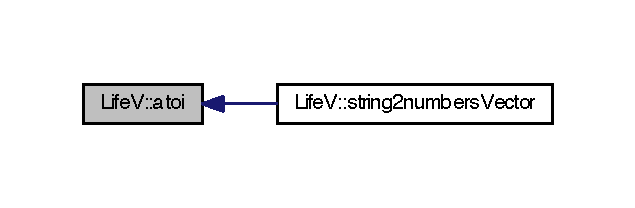
\includegraphics[width=305pt]{namespaceLifeV_a1a787279805886c5b208055992c29c9a_icgraph}
\end{center}
\end{figure}


\hypertarget{namespaceLifeV_aecf5099a32c6f096d09d0506ee79255b}{\index{Life\-V@{Life\-V}!eat\-Comments@{eat\-Comments}}
\index{eat\-Comments@{eat\-Comments}!LifeV@{Life\-V}}
\subsubsection[{eat\-Comments}]{\setlength{\rightskip}{0pt plus 5cm}std\-::istream \& Life\-V\-::eat\-Comments (
\begin{DoxyParamCaption}
\item[{std\-::istream \&}]{s}
\end{DoxyParamCaption}
)}}\label{namespaceLifeV_aecf5099a32c6f096d09d0506ee79255b}


skip lines starting with '!\%\#;\$' 


\begin{DoxyCode}
50 \{
51     \textcolor{keywordtype}{char} \hyperlink{matrici_8m_ae0323a9039add2978bf5b49550572c7c}{c} = \textcolor{charliteral}{'a'};
52     s.get( c ) ;
53     \textcolor{keywordflow}{while} ( c == \textcolor{charliteral}{'!'} ||
54             c == \textcolor{charliteral}{'%'} ||
55             c == \textcolor{charliteral}{'#'} ||
56             c == \textcolor{charliteral}{';'} ||
57             c == \textcolor{charliteral}{'$'} )
58     \{
59         s >> \hyperlink{namespaceLifeV_aa91d4c3fafd93fcbfb7d0aca2b771a02}{eatLine} ;
60         s.get( c ) ;
61     \}
62     \textcolor{keywordflow}{return} s.putback( c ) ;
63 \}\textcolor{comment}{// eatComments}
\end{DoxyCode}


Questo è il grafo delle chiamate per questa funzione\-:\nopagebreak
\begin{figure}[H]
\begin{center}
\leavevmode
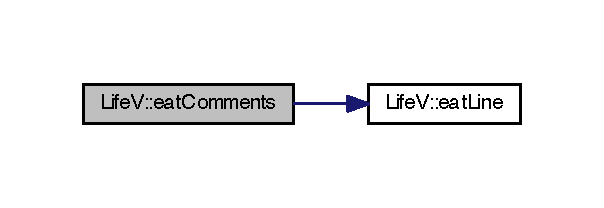
\includegraphics[width=290pt]{namespaceLifeV_aecf5099a32c6f096d09d0506ee79255b_cgraph}
\end{center}
\end{figure}




Questo è il grafo dei chiamanti di questa funzione\-:\nopagebreak
\begin{figure}[H]
\begin{center}
\leavevmode
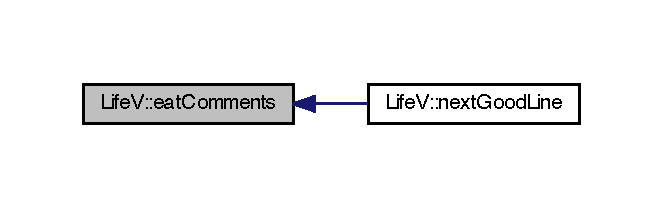
\includegraphics[width=318pt]{namespaceLifeV_aecf5099a32c6f096d09d0506ee79255b_icgraph}
\end{center}
\end{figure}


\hypertarget{namespaceLifeV_aa91d4c3fafd93fcbfb7d0aca2b771a02}{\index{Life\-V@{Life\-V}!eat\-Line@{eat\-Line}}
\index{eat\-Line@{eat\-Line}!LifeV@{Life\-V}}
\subsubsection[{eat\-Line}]{\setlength{\rightskip}{0pt plus 5cm}std\-::istream \& Life\-V\-::eat\-Line (
\begin{DoxyParamCaption}
\item[{std\-::istream \&}]{s}
\end{DoxyParamCaption}
)}}\label{namespaceLifeV_aa91d4c3fafd93fcbfb7d0aca2b771a02}
It gets a the next line from std\-::istream 
\begin{DoxyCode}
42 \{
43     \textcolor{keywordflow}{while} ( s.get() != \textcolor{charliteral}{'\(\backslash\)n'} && s . good() )
44         \{\}
45     \textcolor{keywordflow}{return} s ;
46 \}\textcolor{comment}{// eatLine}
\end{DoxyCode}


Questo è il grafo dei chiamanti di questa funzione\-:\nopagebreak
\begin{figure}[H]
\begin{center}
\leavevmode
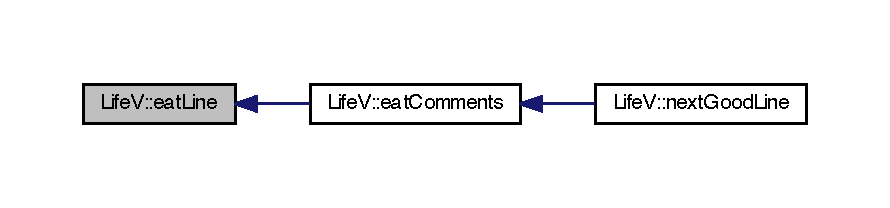
\includegraphics[width=350pt]{namespaceLifeV_aa91d4c3fafd93fcbfb7d0aca2b771a02_icgraph}
\end{center}
\end{figure}


\hypertarget{namespaceLifeV_a2e64a35012f78d9ab021477590e3bfaf}{\index{Life\-V@{Life\-V}!enum2\-String@{enum2\-String}}
\index{enum2\-String@{enum2\-String}!LifeV@{Life\-V}}
\subsubsection[{enum2\-String}]{\setlength{\rightskip}{0pt plus 5cm}template$<$typename Enumerator\-Type $>$ std\-::string Life\-V\-::enum2\-String (
\begin{DoxyParamCaption}
\item[{const Enumerator\-Type \&}]{Enum, }
\item[{const std\-::map$<$ std\-::string, Enumerator\-Type $>$ \&}]{Map}
\end{DoxyParamCaption}
)\hspace{0.3cm}{\ttfamily [inline]}}}\label{namespaceLifeV_a2e64a35012f78d9ab021477590e3bfaf}

\begin{DoxyCode}
147 \{
148     \textcolor{keywordflow}{for} ( \textcolor{keyword}{typename} std::map<std::string, EnumeratorType>::const\_iterator j = Map.begin();
149           j != Map.end() ; ++j )
150         \textcolor{keywordflow}{if} ( j->second == Enum )
151             \textcolor{keywordflow}{return} j->first;
152 
153     \textcolor{keywordflow}{return} \textcolor{stringliteral}{"NO\_TYPE\_FOUND"};
154 \}
\end{DoxyCode}
\hypertarget{namespaceLifeV_a2c4dd8a300964aa48909fce6ad5c72f5}{\index{Life\-V@{Life\-V}!next\-Good\-Line@{next\-Good\-Line}}
\index{next\-Good\-Line@{next\-Good\-Line}!LifeV@{Life\-V}}
\subsubsection[{next\-Good\-Line}]{\setlength{\rightskip}{0pt plus 5cm}std\-::istream \& Life\-V\-::next\-Good\-Line (
\begin{DoxyParamCaption}
\item[{std\-::istream \&}]{s, }
\item[{std\-::string \&}]{line}
\end{DoxyParamCaption}
)}}\label{namespaceLifeV_a2c4dd8a300964aa48909fce6ad5c72f5}


gets next uncommented line 


\begin{DoxyCode}
67 \{
68     s >> \hyperlink{namespaceLifeV_aecf5099a32c6f096d09d0506ee79255b}{eatComments};
69     getline( s, line );
70     \textcolor{keywordflow}{return} s;
71 \}\textcolor{comment}{// nextGoodLine}
\end{DoxyCode}


Questo è il grafo delle chiamate per questa funzione\-:\nopagebreak
\begin{figure}[H]
\begin{center}
\leavevmode
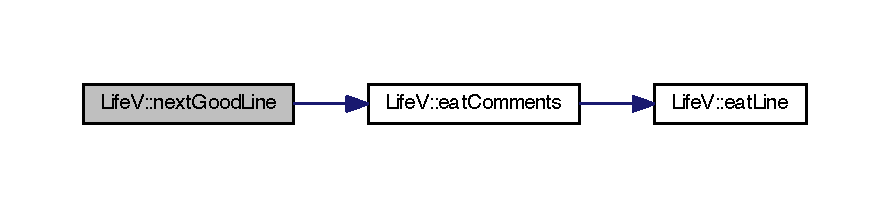
\includegraphics[width=350pt]{namespaceLifeV_a2c4dd8a300964aa48909fce6ad5c72f5_cgraph}
\end{center}
\end{figure}


\hypertarget{namespaceLifeV_a3c2a31cefb08654a69273a1a3bf11fac}{\index{Life\-V@{Life\-V}!number2string@{number2string}}
\index{number2string@{number2string}!LifeV@{Life\-V}}
\subsubsection[{number2string}]{\setlength{\rightskip}{0pt plus 5cm}template$<$typename Number\-Type $>$ std\-::string Life\-V\-::number2string (
\begin{DoxyParamCaption}
\item[{const Number\-Type \&}]{n}
\end{DoxyParamCaption}
)\hspace{0.3cm}{\ttfamily [inline]}}}\label{namespaceLifeV_a3c2a31cefb08654a69273a1a3bf11fac}

\begin{DoxyCode}
134 \{
135     std::stringstream out;
136     out << n;
137 
138     \textcolor{keywordflow}{return} out.str();
139 \}
\end{DoxyCode}
\hypertarget{namespaceLifeV_af57500c586141320ace55cf0b2a5c9fe}{\index{Life\-V@{Life\-V}!operator+@{operator+}}
\index{operator+@{operator+}!LifeV@{Life\-V}}
\subsubsection[{operator+}]{\setlength{\rightskip}{0pt plus 5cm}std\-::string Life\-V\-::operator+ (
\begin{DoxyParamCaption}
\item[{const std\-::string \&}]{str, }
\item[{const int}]{i}
\end{DoxyParamCaption}
)}}\label{namespaceLifeV_af57500c586141320ace55cf0b2a5c9fe}

\begin{DoxyCode}
99 \{
100     \textcolor{keywordtype}{int} digits = abs( \hyperlink{matrici_8m_a6f6ccfcf58b31cb6412107d9d5281426}{i} ) / 10;
101     \textcolor{keywordtype}{char}* str\_i = \textcolor{keyword}{new} \textcolor{keywordtype}{char}[ digits ];
102     sprintf( str\_i, \textcolor{stringliteral}{"%i"}, \hyperlink{matrici_8m_a6f6ccfcf58b31cb6412107d9d5281426}{i} );
103     std::string str2 = str + str\_i;
104     \textcolor{keyword}{delete}[] str\_i;
105     \textcolor{keywordflow}{return} str2;
106 \}\textcolor{comment}{// operator+}
\end{DoxyCode}
\hypertarget{namespaceLifeV_ae00b5ce86e0f837f3f3392074652b7ed}{\index{Life\-V@{Life\-V}!operator+@{operator+}}
\index{operator+@{operator+}!LifeV@{Life\-V}}
\subsubsection[{operator+}]{\setlength{\rightskip}{0pt plus 5cm}std\-::string Life\-V\-::operator+ (
\begin{DoxyParamCaption}
\item[{const std\-::string \&}]{str, }
\item[{const long int}]{i}
\end{DoxyParamCaption}
)}}\label{namespaceLifeV_ae00b5ce86e0f837f3f3392074652b7ed}
\hypertarget{namespaceLifeV_a54f5fa0ff0002920c744bcbaff350bc0}{\index{Life\-V@{Life\-V}!operator+@{operator+}}
\index{operator+@{operator+}!LifeV@{Life\-V}}
\subsubsection[{operator+}]{\setlength{\rightskip}{0pt plus 5cm}std\-::string Life\-V\-::operator+ (
\begin{DoxyParamCaption}
\item[{const std\-::string \&}]{str, }
\item[{const unsigned int}]{i}
\end{DoxyParamCaption}
)}}\label{namespaceLifeV_a54f5fa0ff0002920c744bcbaff350bc0}

\begin{DoxyCode}
120 \{
121     \textcolor{keywordtype}{int} digits = \hyperlink{matrici_8m_a6f6ccfcf58b31cb6412107d9d5281426}{i} / 10;
122     \textcolor{keywordtype}{char}* str\_i = \textcolor{keyword}{new} \textcolor{keywordtype}{char}[ digits ];
123     sprintf( str\_i, \textcolor{stringliteral}{"%u"}, \hyperlink{matrici_8m_a6f6ccfcf58b31cb6412107d9d5281426}{i} );
124     std::string str2 = str + str\_i;
125     \textcolor{keyword}{delete}[] str\_i;
126     \textcolor{keywordflow}{return} str2;
127 \}\textcolor{comment}{// operator+}
\end{DoxyCode}
\hypertarget{namespaceLifeV_aed80af702e5521c5fc90b0c33bbd5af3}{\index{Life\-V@{Life\-V}!operator+@{operator+}}
\index{operator+@{operator+}!LifeV@{Life\-V}}
\subsubsection[{operator+}]{\setlength{\rightskip}{0pt plus 5cm}std\-::string Life\-V\-::operator+ (
\begin{DoxyParamCaption}
\item[{const std\-::string \&}]{str, }
\item[{const long}]{i}
\end{DoxyParamCaption}
)}}\label{namespaceLifeV_aed80af702e5521c5fc90b0c33bbd5af3}

\begin{DoxyCode}
110 \{
111     \textcolor{keywordtype}{int} digits = abs( \hyperlink{matrici_8m_a6f6ccfcf58b31cb6412107d9d5281426}{i} ) / 10;
112     \textcolor{keywordtype}{char}* str\_i = \textcolor{keyword}{new} \textcolor{keywordtype}{char}[ digits ];
113     sprintf( str\_i, \textcolor{stringliteral}{"%ld"}, \hyperlink{matrici_8m_a6f6ccfcf58b31cb6412107d9d5281426}{i} );
114     std::string str2 = str + str\_i;
115     \textcolor{keyword}{delete}[] str\_i;
116     \textcolor{keywordflow}{return} str2;
117 \}\textcolor{comment}{// operator+}
\end{DoxyCode}
\hypertarget{namespaceLifeV_a200b22ebae8c113c2624f7195797d4a4}{\index{Life\-V@{Life\-V}!parse\-List@{parse\-List}}
\index{parse\-List@{parse\-List}!LifeV@{Life\-V}}
\subsubsection[{parse\-List}]{\setlength{\rightskip}{0pt plus 5cm}template$<$typename Entry\-Type $>$ void Life\-V\-::parse\-List (
\begin{DoxyParamCaption}
\item[{const std\-::string \&}]{slist, }
\item[{std\-::list$<$ Entry\-Type $>$ \&}]{list}
\end{DoxyParamCaption}
)}}\label{namespaceLifeV_a200b22ebae8c113c2624f7195797d4a4}

\begin{DoxyCode}
92 \{
93     std::string stringList = slist;
94     \textcolor{keywordflow}{if} ( slist == \textcolor{stringliteral}{""} )
95     \{
96         \textcolor{keywordflow}{return};
97     \}
98 
99     \textcolor{keywordtype}{int} commaPos = 0;
100 
101     \textcolor{keywordflow}{while} ( commaPos != (\textcolor{keywordtype}{int})std::string::npos )
102     \{
103         commaPos = stringList.find( \textcolor{stringliteral}{","} );
104 
105         std::stringstream stream;
106         stream <<  stringList.substr( 0, commaPos ).c\_str();
107 
108         EntryType var;
109         stream >> var;
110         list.push\_back( var );
111 
112         stringList = stringList.substr( commaPos + 1 );
113     \}
114 \}
\end{DoxyCode}
\hypertarget{namespaceLifeV_a5fb0107fd71b5be2c32f536619a73175}{\index{Life\-V@{Life\-V}!set\-String\-Length@{set\-String\-Length}}
\index{set\-String\-Length@{set\-String\-Length}!LifeV@{Life\-V}}
\subsubsection[{set\-String\-Length}]{\setlength{\rightskip}{0pt plus 5cm}std\-::string \& Life\-V\-::set\-String\-Length (
\begin{DoxyParamCaption}
\item[{std\-::string \&}]{s, }
\item[{unsigned int}]{len, }
\item[{char}]{c}
\end{DoxyParamCaption}
)}}\label{namespaceLifeV_a5fb0107fd71b5be2c32f536619a73175}
always return a std\-::string with len characters
\begin{DoxyItemize}
\item if the s has more than len characters \-: keep only the first len
\item if the s has less than len characters \-: complete with c until len 
\end{DoxyItemize}
\begin{DoxyCode}
75 \{
76     \textcolor{comment}{/*}
77 \textcolor{comment}{      always return a std::string with len characters}
78 \textcolor{comment}{        - if the s has more than len characters : keep only the first len}
79 \textcolor{comment}{        - if the s has less than len characters : complete with c until len}
80 \textcolor{comment}{    */}
81     std::string stmp( len, \hyperlink{matrici_8m_ae0323a9039add2978bf5b49550572c7c}{c} );
82     \textcolor{keywordflow}{if} ( s.length() > len )
83     \{
84         s.erase( len, s.length() );
85     \}
86     stmp.replace( 0, s.length(), s );
87     s = stmp;
88     \textcolor{keywordflow}{return} s;
89 \}\textcolor{comment}{// setStringLength}
\end{DoxyCode}
\hypertarget{namespaceLifeV_a95341022bde9111ea53dfe204cbe70ae}{\index{Life\-V@{Life\-V}!string2number@{string2number}}
\index{string2number@{string2number}!LifeV@{Life\-V}}
\subsubsection[{string2number}]{\setlength{\rightskip}{0pt plus 5cm}double Life\-V\-::string2number (
\begin{DoxyParamCaption}
\item[{const std\-::string \&}]{s}
\end{DoxyParamCaption}
)\hspace{0.3cm}{\ttfamily [inline]}}}\label{namespaceLifeV_a95341022bde9111ea53dfe204cbe70ae}

\begin{DoxyCode}
120 \{
121     std::stringstream out;
122     out << s;
123 
124     \textcolor{keywordtype}{double} n;
125     out >> n;
126 
127     \textcolor{keywordflow}{return} n;
128 \}
\end{DoxyCode}
\hypertarget{namespaceLifeV_a5f2c3319750ceebbeb2a3bb374a2596b}{\index{Life\-V@{Life\-V}!string2numbers\-Vector@{string2numbers\-Vector}}
\index{string2numbers\-Vector@{string2numbers\-Vector}!LifeV@{Life\-V}}
\subsubsection[{string2numbers\-Vector}]{\setlength{\rightskip}{0pt plus 5cm}template$<$typename Number\-Type $>$ void Life\-V\-::string2numbers\-Vector (
\begin{DoxyParamCaption}
\item[{const std\-::string \&}]{string, }
\item[{std\-::vector$<$ Number\-Type $>$ \&}]{number\-Vector}
\end{DoxyParamCaption}
)}}\label{namespaceLifeV_a5f2c3319750ceebbeb2a3bb374a2596b}

\begin{DoxyCode}
161 \{
162     \textcolor{comment}{//Split the string}
163     std::vector< std::string > stringVector;
164     boost::split( stringVector, \textcolor{keywordtype}{string}, boost::is\_any\_of( \textcolor{stringliteral}{","} ) );
165 
166     \textcolor{comment}{//Convert to the right type}
167     \textcolor{keywordflow}{for} ( \hyperlink{namespaceLifeV_a4bd093cf6b0d5b57b2d89e0e90d610b7}{UInt} \hyperlink{matrici_8m_a6f6ccfcf58b31cb6412107d9d5281426}{i}( 0 ); i < static\_cast<UInt> ( stringVector.size() ); ++\hyperlink{matrici_8m_a6f6ccfcf58b31cb6412107d9d5281426}{i} )
168         numberVector.push\_back( static\_cast<NumberType>( \hyperlink{namespaceLifeV_a1a787279805886c5b208055992c29c9a}{std::atoi}( stringVector[
      \hyperlink{matrici_8m_a6f6ccfcf58b31cb6412107d9d5281426}{i}].c\_str())));
169 \}
\end{DoxyCode}


Questo è il grafo delle chiamate per questa funzione\-:\nopagebreak
\begin{figure}[H]
\begin{center}
\leavevmode
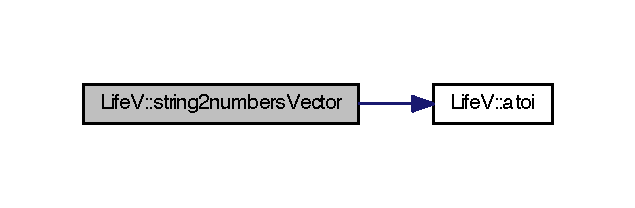
\includegraphics[width=305pt]{namespaceLifeV_a5f2c3319750ceebbeb2a3bb374a2596b_cgraph}
\end{center}
\end{figure}



\chapter{Documentazione delle classi}
\hypertarget{classBC}{\section{Riferimenti per la classe B\-C}
\label{classBC}\index{B\-C@{B\-C}}
}


\hyperlink{BC_8h}{B\-C.\-h}.  




{\ttfamily \#include $<$B\-C.\-h$>$}

\subsection*{Tipi pubblici}
\begin{DoxyCompactItemize}
\item 
enum \{ \hyperlink{classBC_ad1b507696802f73b95c0ca59f4c41390a99103ccd54ba29b1bd2670cc6cd0c462}{D\-I\-R\-I\-C\-H\-L\-E\-T\-\_\-\-B\-O\-U\-N\-D\-A\-R\-Y\-\_\-\-N\-U\-M} = 40, 
\hyperlink{classBC_ad1b507696802f73b95c0ca59f4c41390a432aa77a00d8eb4929463ef8d57b5c04}{N\-E\-U\-M\-A\-N\-N\-\_\-\-B\-O\-U\-N\-D\-A\-R\-Y\-\_\-\-N\-U\-M} = 50
 \}
\end{DoxyCompactItemize}
\subsection*{Membri pubblici}
\begin{DoxyCompactItemize}
\item 
\hyperlink{classBC_a75c13d0876a8230d1ec702341182da1c}{B\-C} (getfem\-::mesh \&mesh, const std\-::string \&Mesh\-Type, const \hyperlink{Core_8h_a419d7707e418f02d8daeb1fc7c0b9ae5}{Element\-Dimension} \&dimension=\hyperlink{Core_8h_a419d7707e418f02d8daeb1fc7c0b9ae5a5340ec7ecef6cc3886684a3bd3450d64}{M\-E\-D\-I\-U\-M})
\begin{DoxyCompactList}\small\item\em \hyperlink{BC_8cc}{B\-C.\-cc}. \end{DoxyCompactList}\item 
const \hyperlink{Core_8h_a83c51913d041a5001e8683434c09857f}{size\-Vector\-\_\-\-Type} \& \hyperlink{classBC_af2d22ae9848e3bed61f2106610bde5b7}{get\-Dirichlet} () const 
\item 
const size\-\_\-type \& \hyperlink{classBC_ae61f04dfbb377e38e4c43e0516e51c36}{get\-Dirichlet} (const size\-\_\-type \&dof) const 
\item 
const \hyperlink{Core_8h_a83c51913d041a5001e8683434c09857f}{size\-Vector\-\_\-\-Type} \& \hyperlink{classBC_a9541adfa180ca9783052349c373b0228}{get\-Neumann} () const 
\item 
const size\-\_\-type \& \hyperlink{classBC_a88bd7cd141cda536ce128f13b17d61b5}{get\-Neumann} (const size\-\_\-type \&dof) const 
\item 
const getfem\-::mesh\-\_\-fem \& \hyperlink{classBC_a920bf87c4fe5c10289923859f3ca7afc}{get\-Mesh\-F\-E\-M} () const 
\end{DoxyCompactItemize}


\subsection{Descrizione dettagliata}
\hyperlink{BC_8h}{B\-C.\-h}. 

Libreria che introduce le condizioni al bordo sul problema

Created on\-: Apr 11, 2011

Author\-: fumagalli 

\subsection{Documentazione dei tipi enumerati (enum)}
\hypertarget{classBC_ad1b507696802f73b95c0ca59f4c41390}{\subsubsection[{anonymous enum}]{\setlength{\rightskip}{0pt plus 5cm}anonymous enum}}\label{classBC_ad1b507696802f73b95c0ca59f4c41390}
\begin{Desc}
\item[Valori del tipo enumerato]\par
\begin{description}
\index{D\-I\-R\-I\-C\-H\-L\-E\-T\-\_\-\-B\-O\-U\-N\-D\-A\-R\-Y\-\_\-\-N\-U\-M@{D\-I\-R\-I\-C\-H\-L\-E\-T\-\_\-\-B\-O\-U\-N\-D\-A\-R\-Y\-\_\-\-N\-U\-M}!B\-C@{B\-C}}\index{B\-C@{B\-C}!D\-I\-R\-I\-C\-H\-L\-E\-T\-\_\-\-B\-O\-U\-N\-D\-A\-R\-Y\-\_\-\-N\-U\-M@{D\-I\-R\-I\-C\-H\-L\-E\-T\-\_\-\-B\-O\-U\-N\-D\-A\-R\-Y\-\_\-\-N\-U\-M}}\item[{\em 
\hypertarget{classBC_ad1b507696802f73b95c0ca59f4c41390a99103ccd54ba29b1bd2670cc6cd0c462}{D\-I\-R\-I\-C\-H\-L\-E\-T\-\_\-\-B\-O\-U\-N\-D\-A\-R\-Y\-\_\-\-N\-U\-M}\label{classBC_ad1b507696802f73b95c0ca59f4c41390a99103ccd54ba29b1bd2670cc6cd0c462}
}]\index{N\-E\-U\-M\-A\-N\-N\-\_\-\-B\-O\-U\-N\-D\-A\-R\-Y\-\_\-\-N\-U\-M@{N\-E\-U\-M\-A\-N\-N\-\_\-\-B\-O\-U\-N\-D\-A\-R\-Y\-\_\-\-N\-U\-M}!B\-C@{B\-C}}\index{B\-C@{B\-C}!N\-E\-U\-M\-A\-N\-N\-\_\-\-B\-O\-U\-N\-D\-A\-R\-Y\-\_\-\-N\-U\-M@{N\-E\-U\-M\-A\-N\-N\-\_\-\-B\-O\-U\-N\-D\-A\-R\-Y\-\_\-\-N\-U\-M}}\item[{\em 
\hypertarget{classBC_ad1b507696802f73b95c0ca59f4c41390a432aa77a00d8eb4929463ef8d57b5c04}{N\-E\-U\-M\-A\-N\-N\-\_\-\-B\-O\-U\-N\-D\-A\-R\-Y\-\_\-\-N\-U\-M}\label{classBC_ad1b507696802f73b95c0ca59f4c41390a432aa77a00d8eb4929463ef8d57b5c04}
}]\end{description}
\end{Desc}

\begin{DoxyCode}
23     \{
24         \hyperlink{classBC_ad1b507696802f73b95c0ca59f4c41390a99103ccd54ba29b1bd2670cc6cd0c462}{DIRICHLET\_BOUNDARY\_NUM} = 40,
25         \hyperlink{classBC_ad1b507696802f73b95c0ca59f4c41390a432aa77a00d8eb4929463ef8d57b5c04}{NEUMANN\_BOUNDARY\_NUM} = 50
26     \};
\end{DoxyCode}


\subsection{Documentazione dei costruttori e dei distruttori}
\hypertarget{classBC_a75c13d0876a8230d1ec702341182da1c}{\index{B\-C@{B\-C}!B\-C@{B\-C}}
\index{B\-C@{B\-C}!BC@{B\-C}}
\subsubsection[{B\-C}]{\setlength{\rightskip}{0pt plus 5cm}B\-C\-::\-B\-C (
\begin{DoxyParamCaption}
\item[{getfem\-::mesh \&}]{mesh, }
\item[{const std\-::string \&}]{Mesh\-Type, }
\item[{const {\bf Element\-Dimension} \&}]{dimension = {\ttfamily {\bf M\-E\-D\-I\-U\-M}}}
\end{DoxyParamCaption}
)}}\label{classBC_a75c13d0876a8230d1ec702341182da1c}


\hyperlink{BC_8cc}{B\-C.\-cc}. 

Libreria che introduce le condizioni al bordo sul problema

Created on\-: Apr 11, 2011

Author\-: fumagalli 
\begin{DoxyCode}
16                                              :
17     M\_meshFEM(mesh)
18 \{
19 
20     \textcolor{comment}{// Dual variable spaces}
21     \textcolor{comment}{//getfem::pfem FETypePressure = getfem::fem\_descriptor(FEMType);}
22 
23     \textcolor{comment}{//M\_meshFEM.set\_finite\_element(mesh.convex\_index(), FETypePressure);}
24     bgeot::pgeometric\_trans geometricTransformation;
25 
26     geometricTransformation = bgeot::geometric\_trans\_descriptor(MeshType);
27 
28     M\_meshFEM.set\_finite\_element(mesh.convex\_index(), getfem::classical\_fem(
29             geometricTransformation, 1));
30 
31     \textcolor{comment}{// Flag for fracture boundary conditions}
32     \textcolor{comment}{// Dirichlet boundary condition}
33     M\_dirichlet.clear();
34     M\_dirichlet.push\_back(\hyperlink{classBC_ad1b507696802f73b95c0ca59f4c41390a99103ccd54ba29b1bd2670cc6cd0c462}{DIRICHLET\_BOUNDARY\_NUM});
35 
36     \textcolor{comment}{// Neumann boundary condition}
37     M\_neumann.clear();
38     M\_neumann.push\_back(\hyperlink{classBC_ad1b507696802f73b95c0ca59f4c41390a432aa77a00d8eb4929463ef8d57b5c04}{NEUMANN\_BOUNDARY\_NUM});
39 
40     \textcolor{comment}{// All boundary conditions}
41     M\_extBoundary.clear();
42     M\_extBoundary.push\_back(\hyperlink{classBC_ad1b507696802f73b95c0ca59f4c41390a99103ccd54ba29b1bd2670cc6cd0c462}{DIRICHLET\_BOUNDARY\_NUM});
43     M\_extBoundary.push\_back(\hyperlink{classBC_ad1b507696802f73b95c0ca59f4c41390a432aa77a00d8eb4929463ef8d57b5c04}{NEUMANN\_BOUNDARY\_NUM});
44 
45     \hyperlink{Core_8h_a83c51913d041a5001e8683434c09857f}{sizeVector\_Type} boundaryFlags(2);
46     boundaryFlags [ 0 ] = \hyperlink{classBC_ad1b507696802f73b95c0ca59f4c41390a99103ccd54ba29b1bd2670cc6cd0c462}{DIRICHLET\_BOUNDARY\_NUM};
47     boundaryFlags [ 1 ] = \hyperlink{classBC_ad1b507696802f73b95c0ca59f4c41390a432aa77a00d8eb4929463ef8d57b5c04}{NEUMANN\_BOUNDARY\_NUM};
48 
49     \hyperlink{Core_8h_a80e8381d86ecb0a7f4f87ff84d1a0be5}{sizeVectorContainer\_Type} boundary\_cv;
50     \hyperlink{Core_8h_a80e8381d86ecb0a7f4f87ff84d1a0be5}{sizeVectorContainer\_Type} boundary\_flags;
51 
52     \textcolor{comment}{// Number of Neumann boundary condition}
53     size\_type neumannBoundary = 0;
54 
55     \textcolor{comment}{// List all the convexes}
56     dal::bit\_vector nn = mesh.convex\_index();
57     bgeot::size\_type i\_cv;
58 
59     \textcolor{keywordflow}{for} ( i\_cv << nn; i\_cv != bgeot::size\_type(-1); i\_cv << nn )
60     \{
61         neumannBoundary++;
62     \}
63 
64     boundary\_cv.resize(neumannBoundary);
65     boundary\_flags.resize(neumannBoundary);
66 
67     getfem::mesh\_region borderFaces;
68     getfem::outer\_faces\_of\_mesh(mesh, borderFaces);
69 
70     \textcolor{keywordflow}{if} ( dimension == \hyperlink{Core_8h_a419d7707e418f02d8daeb1fc7c0b9ae5a5340ec7ecef6cc3886684a3bd3450d64}{MEDIUM} )
71     \{
72         \textcolor{keywordflow}{for} ( getfem::mr\_visitor i(borderFaces); !i.finished(); ++i )
73         \{
74             assert(i.is\_face());
75 
76             base\_node un = mesh.normal\_of\_face\_of\_convex(i.cv(), i.f());
77             un /= gmm::vect\_norm2(un);
78 
79             \textcolor{keywordflow}{if}  (\textcolor{keyword}{false})  \textcolor{comment}{//( gmm::abs(gmm::abs(un [ dimension - 1 ]) - 1.0) > 1.0E-7 )}
80             \{
81                 \textcolor{comment}{// Dirichlet, flag 0}
82                 boundary\_cv [ i.cv() ].push\_back(i.f());
83                 boundary\_flags [ i.cv() ].push\_back(boundaryFlags [ 0 ]);
84                 \textcolor{comment}{//This        will enforce M\_mediumMesh.region(0).add(i.cv(), i.f());}
85             \}
86             \textcolor{keywordflow}{else}
87             \{
88                 \textcolor{comment}{// Neumann, flag 1}
89                 boundary\_cv [ i.cv() ].push\_back(i.f());
90                 boundary\_flags [ i.cv() ].push\_back(boundaryFlags [ 1 ]);
91                 \textcolor{comment}{// This will enforce M\_mediumMesh.region(1).add(i.cv(), i.f());}
92             \}
93         \}
94     \}
95     \textcolor{keywordflow}{else}
96     \{
97 
98         \textcolor{keywordflow}{for} ( getfem::mr\_visitor i(borderFaces); !i.finished(); ++i )
99         \{
100             assert(i.is\_face());
101             base\_node un = mesh.normal\_of\_face\_of\_convex(i.cv(), i.f());
102             un /= gmm::vect\_norm2(un);
103 
104             \textcolor{keywordflow}{if} (\textcolor{keyword}{false})\textcolor{comment}{//( gmm::abs(gmm::abs(un [ dimension - 1 ]) - 1.0) > 1.0E-7 )}
105             \{
106             \textcolor{comment}{// Dirichlet, flag 0}
107             boundary\_cv [ i.cv() ].push\_back(i.f());
108             boundary\_flags [ i.cv() ].push\_back(boundaryFlags [ 1 ]);
109             \textcolor{comment}{//This        will enforce M\_mediumMesh.region(0).add(i.cv(), i.f());}
110         \}
111         \textcolor{keywordflow}{else}
112             \{
113                 \textcolor{comment}{// Neumann, flag 1}
114                 boundary\_cv [ i.cv() ].push\_back(i.f());
115                 boundary\_flags [ i.cv() ].push\_back(boundaryFlags [1 ]);
116                 \textcolor{comment}{// This will enforce M\_mediumMesh.region(1).add(i.cv(), i.f());}
117             \}
118         \}
119     \}
120     \textcolor{comment}{// Bulk mesh}
121     \textcolor{keywordflow}{for} ( size\_type cv = 0; cv < boundary\_flags.size(); ++cv )
122     \{
123         \textcolor{keywordflow}{for} ( size\_type j = 0; j < boundary\_flags [ cv ].size(); j++ )
124         \{
125             mesh.region(boundary\_flags [ cv ] [ j ]).add(cv,
126                     boundary\_cv [ cv ] [ j ]);
127         \}
128     \}
129 
130 \}\textcolor{comment}{// costruttore}
\end{DoxyCode}


\subsection{Documentazione delle funzioni membro}
\hypertarget{classBC_af2d22ae9848e3bed61f2106610bde5b7}{\index{B\-C@{B\-C}!get\-Dirichlet@{get\-Dirichlet}}
\index{get\-Dirichlet@{get\-Dirichlet}!BC@{B\-C}}
\subsubsection[{get\-Dirichlet}]{\setlength{\rightskip}{0pt plus 5cm}const {\bf size\-Vector\-\_\-\-Type}\& B\-C\-::get\-Dirichlet (
\begin{DoxyParamCaption}
{}
\end{DoxyParamCaption}
) const\hspace{0.3cm}{\ttfamily [inline]}}}\label{classBC_af2d22ae9848e3bed61f2106610bde5b7}

\begin{DoxyCode}
36     \{
37         \textcolor{keywordflow}{return} M\_dirichlet;
38     \}
\end{DoxyCode}
\hypertarget{classBC_ae61f04dfbb377e38e4c43e0516e51c36}{\index{B\-C@{B\-C}!get\-Dirichlet@{get\-Dirichlet}}
\index{get\-Dirichlet@{get\-Dirichlet}!BC@{B\-C}}
\subsubsection[{get\-Dirichlet}]{\setlength{\rightskip}{0pt plus 5cm}const size\-\_\-type\& B\-C\-::get\-Dirichlet (
\begin{DoxyParamCaption}
\item[{const size\-\_\-type \&}]{dof}
\end{DoxyParamCaption}
) const\hspace{0.3cm}{\ttfamily [inline]}}}\label{classBC_ae61f04dfbb377e38e4c43e0516e51c36}

\begin{DoxyCode}
42     \{
43         \textcolor{keywordflow}{return} M\_dirichlet [ dof ];
44     \}
\end{DoxyCode}
\hypertarget{classBC_a920bf87c4fe5c10289923859f3ca7afc}{\index{B\-C@{B\-C}!get\-Mesh\-F\-E\-M@{get\-Mesh\-F\-E\-M}}
\index{get\-Mesh\-F\-E\-M@{get\-Mesh\-F\-E\-M}!BC@{B\-C}}
\subsubsection[{get\-Mesh\-F\-E\-M}]{\setlength{\rightskip}{0pt plus 5cm}const getfem\-::mesh\-\_\-fem\& B\-C\-::get\-Mesh\-F\-E\-M (
\begin{DoxyParamCaption}
{}
\end{DoxyParamCaption}
) const\hspace{0.3cm}{\ttfamily [inline]}}}\label{classBC_a920bf87c4fe5c10289923859f3ca7afc}

\begin{DoxyCode}
60     \{
61         \textcolor{keywordflow}{return} M\_meshFEM;
62     \}
\end{DoxyCode}
\hypertarget{classBC_a9541adfa180ca9783052349c373b0228}{\index{B\-C@{B\-C}!get\-Neumann@{get\-Neumann}}
\index{get\-Neumann@{get\-Neumann}!BC@{B\-C}}
\subsubsection[{get\-Neumann}]{\setlength{\rightskip}{0pt plus 5cm}const {\bf size\-Vector\-\_\-\-Type}\& B\-C\-::get\-Neumann (
\begin{DoxyParamCaption}
{}
\end{DoxyParamCaption}
) const\hspace{0.3cm}{\ttfamily [inline]}}}\label{classBC_a9541adfa180ca9783052349c373b0228}

\begin{DoxyCode}
48     \{
49         \textcolor{keywordflow}{return} M\_neumann;
50     \}
\end{DoxyCode}
\hypertarget{classBC_a88bd7cd141cda536ce128f13b17d61b5}{\index{B\-C@{B\-C}!get\-Neumann@{get\-Neumann}}
\index{get\-Neumann@{get\-Neumann}!BC@{B\-C}}
\subsubsection[{get\-Neumann}]{\setlength{\rightskip}{0pt plus 5cm}const size\-\_\-type\& B\-C\-::get\-Neumann (
\begin{DoxyParamCaption}
\item[{const size\-\_\-type \&}]{dof}
\end{DoxyParamCaption}
) const\hspace{0.3cm}{\ttfamily [inline]}}}\label{classBC_a88bd7cd141cda536ce128f13b17d61b5}

\begin{DoxyCode}
54     \{
55         \textcolor{keywordflow}{return} M\_neumann [ dof ];
56     \}
\end{DoxyCode}


La documentazione per questa classe è stata generata a partire dai seguenti file\-:\begin{DoxyCompactItemize}
\item 
include/\hyperlink{BC_8h}{B\-C.\-h}\item 
src/\hyperlink{BC_8cc}{B\-C.\-cc}\end{DoxyCompactItemize}

\hypertarget{classBCHandler}{\section{Riferimenti per la classe B\-C\-Handler}
\label{classBCHandler}\index{B\-C\-Handler@{B\-C\-Handler}}
}


\hyperlink{BCHandler_8h}{B\-C\-Handler.\-h}.  




{\ttfamily \#include $<$B\-C\-Handler.\-h$>$}

\subsection*{Tipi pubblici}
\begin{DoxyCompactItemize}
\item 
enum \{ \hyperlink{classBCHandler_a2bc86209db0836dbc6ca56e1ca4e4ac1a57ea96455b2ba998cc42a21aa7e1d842}{D\-I\-R\-I\-C\-H\-L\-E\-T\-\_\-\-B\-O\-U\-N\-D\-A\-R\-Y\-\_\-\-C\-U\-T} = 400, 
\hyperlink{classBCHandler_a2bc86209db0836dbc6ca56e1ca4e4ac1add7397a06718591b0c27c067225b1d5f}{N\-E\-U\-M\-A\-N\-N\-\_\-\-B\-O\-U\-N\-D\-A\-R\-Y\-\_\-\-C\-U\-T} = 500, 
\hyperlink{classBCHandler_a2bc86209db0836dbc6ca56e1ca4e4ac1a487ba8af2086045d8b0df840b2525866}{D\-I\-R\-I\-C\-H\-L\-E\-T\-\_\-\-B\-O\-U\-N\-D\-A\-R\-Y\-\_\-\-U\-N\-C\-U\-T} = 4000, 
\hyperlink{classBCHandler_a2bc86209db0836dbc6ca56e1ca4e4ac1aa538eee48606669ac37073ca65144007}{N\-E\-U\-M\-A\-N\-N\-\_\-\-B\-O\-U\-N\-D\-A\-R\-Y\-\_\-\-U\-N\-C\-U\-T} = 5000
 \}
\end{DoxyCompactItemize}
\subsection*{Membri pubblici}
\begin{DoxyCompactItemize}
\item 
\hyperlink{classBCHandler_a35bb263a58e1bc9e0cfd34bf9cffac0d}{B\-C\-Handler} (const \hyperlink{BC_8h_a088c36f945ad8f6e7e0c7c423994c6ec}{B\-C\-Ptr\-\_\-\-Type} \&medium\-B\-C, const \hyperlink{BC_8h_ae127263052e0676d0fe233f834ca7227}{B\-C\-Ptr\-Container\-\_\-\-Type} \&fracture\-B\-C)
\begin{DoxyCompactList}\small\item\em \hyperlink{BCHandler_8cc}{B\-C\-Handler.\-cc}. \end{DoxyCompactList}\item 
void \hyperlink{classBCHandler_a1dcccdbb5e0eb0d044455414b52b2f05}{create\-B\-D\-Regions} (getfem\-::mesh \&mesh)
\item 
void \hyperlink{classBCHandler_a559e4ba01fc7c6326dbb949d06dbd525}{create\-B\-D\-Regions\-Fractures} (getfem\-::mesh \&mesh)
\item 
const \hyperlink{BC_8h_a088c36f945ad8f6e7e0c7c423994c6ec}{B\-C\-Ptr\-\_\-\-Type} \& \hyperlink{classBCHandler_ab7e56a166f8f51be96b2bf8946bf7b62}{get\-Medium\-B\-C} () const 
\item 
const \hyperlink{BC_8h_a088c36f945ad8f6e7e0c7c423994c6ec}{B\-C\-Ptr\-\_\-\-Type} \& \hyperlink{classBCHandler_a2ab65711f8ee3643ecf19de52ceab470}{get\-Fracture\-B\-C} (const size\-\_\-type \&id) const 
\item 
const \hyperlink{Core_8h_a83c51913d041a5001e8683434c09857f}{size\-Vector\-\_\-\-Type} \& \hyperlink{classBCHandler_a68a01c71517202ed89ebc82a56e4cb5d}{get\-Dirichlet\-Uncut} () const 
\item 
const size\-\_\-type \& \hyperlink{classBCHandler_a3f92a68c9b0dbebc6ee72a42b419645d}{get\-Dirichlet\-Uncut} (const size\-\_\-type \&dof) const 
\item 
const \hyperlink{Core_8h_a83c51913d041a5001e8683434c09857f}{size\-Vector\-\_\-\-Type} \& \hyperlink{classBCHandler_a5b1c86a6c303abf33850132d1bc12693}{get\-Neumann\-Uncut} () const 
\item 
const size\-\_\-type \& \hyperlink{classBCHandler_a2bf41619c541b124b421d8664786a055}{get\-Neumann\-Uncut} (const size\-\_\-type \&dof) const 
\item 
const \hyperlink{Core_8h_a83c51913d041a5001e8683434c09857f}{size\-Vector\-\_\-\-Type} \& \hyperlink{classBCHandler_a1efb6389dbecbcd38e53422ffc6f29c7}{get\-Dirichlet\-Cut} (const size\-\_\-type \&id) const 
\item 
const size\-\_\-type \& \hyperlink{classBCHandler_a390cb50c5fcbbf2e676fe7d5f5241180}{get\-Dirichlet\-Cut} (const size\-\_\-type \&id, const size\-\_\-type \&dof) const 
\item 
const \hyperlink{Core_8h_a83c51913d041a5001e8683434c09857f}{size\-Vector\-\_\-\-Type} \& \hyperlink{classBCHandler_a5e71b2adeaa281e88275bff504dc67d8}{get\-Neumann\-Cut} (const size\-\_\-type \&id) const 
\item 
const size\-\_\-type \& \hyperlink{classBCHandler_a726f1bfbc76113bbb3b5057b25a53871}{get\-Neumann\-Cut} (const size\-\_\-type \&id, const size\-\_\-type \&dof) const 
\end{DoxyCompactItemize}


\subsection{Descrizione dettagliata}
\hyperlink{BCHandler_8h}{B\-C\-Handler.\-h}. 

Libreria che gestisce le condizioni al bordo nella mesh

Created on\-: Apr 5, 2011

Author\-: fumagalli 

\subsection{Documentazione dei tipi enumerati (enum)}
\hypertarget{classBCHandler_a2bc86209db0836dbc6ca56e1ca4e4ac1}{\subsubsection[{anonymous enum}]{\setlength{\rightskip}{0pt plus 5cm}anonymous enum}}\label{classBCHandler_a2bc86209db0836dbc6ca56e1ca4e4ac1}
\begin{Desc}
\item[Valori del tipo enumerato]\par
\begin{description}
\index{D\-I\-R\-I\-C\-H\-L\-E\-T\-\_\-\-B\-O\-U\-N\-D\-A\-R\-Y\-\_\-\-C\-U\-T@{D\-I\-R\-I\-C\-H\-L\-E\-T\-\_\-\-B\-O\-U\-N\-D\-A\-R\-Y\-\_\-\-C\-U\-T}!B\-C\-Handler@{B\-C\-Handler}}\index{B\-C\-Handler@{B\-C\-Handler}!D\-I\-R\-I\-C\-H\-L\-E\-T\-\_\-\-B\-O\-U\-N\-D\-A\-R\-Y\-\_\-\-C\-U\-T@{D\-I\-R\-I\-C\-H\-L\-E\-T\-\_\-\-B\-O\-U\-N\-D\-A\-R\-Y\-\_\-\-C\-U\-T}}\item[{\em 
\hypertarget{classBCHandler_a2bc86209db0836dbc6ca56e1ca4e4ac1a57ea96455b2ba998cc42a21aa7e1d842}{D\-I\-R\-I\-C\-H\-L\-E\-T\-\_\-\-B\-O\-U\-N\-D\-A\-R\-Y\-\_\-\-C\-U\-T}\label{classBCHandler_a2bc86209db0836dbc6ca56e1ca4e4ac1a57ea96455b2ba998cc42a21aa7e1d842}
}]\index{N\-E\-U\-M\-A\-N\-N\-\_\-\-B\-O\-U\-N\-D\-A\-R\-Y\-\_\-\-C\-U\-T@{N\-E\-U\-M\-A\-N\-N\-\_\-\-B\-O\-U\-N\-D\-A\-R\-Y\-\_\-\-C\-U\-T}!B\-C\-Handler@{B\-C\-Handler}}\index{B\-C\-Handler@{B\-C\-Handler}!N\-E\-U\-M\-A\-N\-N\-\_\-\-B\-O\-U\-N\-D\-A\-R\-Y\-\_\-\-C\-U\-T@{N\-E\-U\-M\-A\-N\-N\-\_\-\-B\-O\-U\-N\-D\-A\-R\-Y\-\_\-\-C\-U\-T}}\item[{\em 
\hypertarget{classBCHandler_a2bc86209db0836dbc6ca56e1ca4e4ac1add7397a06718591b0c27c067225b1d5f}{N\-E\-U\-M\-A\-N\-N\-\_\-\-B\-O\-U\-N\-D\-A\-R\-Y\-\_\-\-C\-U\-T}\label{classBCHandler_a2bc86209db0836dbc6ca56e1ca4e4ac1add7397a06718591b0c27c067225b1d5f}
}]\index{D\-I\-R\-I\-C\-H\-L\-E\-T\-\_\-\-B\-O\-U\-N\-D\-A\-R\-Y\-\_\-\-U\-N\-C\-U\-T@{D\-I\-R\-I\-C\-H\-L\-E\-T\-\_\-\-B\-O\-U\-N\-D\-A\-R\-Y\-\_\-\-U\-N\-C\-U\-T}!B\-C\-Handler@{B\-C\-Handler}}\index{B\-C\-Handler@{B\-C\-Handler}!D\-I\-R\-I\-C\-H\-L\-E\-T\-\_\-\-B\-O\-U\-N\-D\-A\-R\-Y\-\_\-\-U\-N\-C\-U\-T@{D\-I\-R\-I\-C\-H\-L\-E\-T\-\_\-\-B\-O\-U\-N\-D\-A\-R\-Y\-\_\-\-U\-N\-C\-U\-T}}\item[{\em 
\hypertarget{classBCHandler_a2bc86209db0836dbc6ca56e1ca4e4ac1a487ba8af2086045d8b0df840b2525866}{D\-I\-R\-I\-C\-H\-L\-E\-T\-\_\-\-B\-O\-U\-N\-D\-A\-R\-Y\-\_\-\-U\-N\-C\-U\-T}\label{classBCHandler_a2bc86209db0836dbc6ca56e1ca4e4ac1a487ba8af2086045d8b0df840b2525866}
}]\index{N\-E\-U\-M\-A\-N\-N\-\_\-\-B\-O\-U\-N\-D\-A\-R\-Y\-\_\-\-U\-N\-C\-U\-T@{N\-E\-U\-M\-A\-N\-N\-\_\-\-B\-O\-U\-N\-D\-A\-R\-Y\-\_\-\-U\-N\-C\-U\-T}!B\-C\-Handler@{B\-C\-Handler}}\index{B\-C\-Handler@{B\-C\-Handler}!N\-E\-U\-M\-A\-N\-N\-\_\-\-B\-O\-U\-N\-D\-A\-R\-Y\-\_\-\-U\-N\-C\-U\-T@{N\-E\-U\-M\-A\-N\-N\-\_\-\-B\-O\-U\-N\-D\-A\-R\-Y\-\_\-\-U\-N\-C\-U\-T}}\item[{\em 
\hypertarget{classBCHandler_a2bc86209db0836dbc6ca56e1ca4e4ac1aa538eee48606669ac37073ca65144007}{N\-E\-U\-M\-A\-N\-N\-\_\-\-B\-O\-U\-N\-D\-A\-R\-Y\-\_\-\-U\-N\-C\-U\-T}\label{classBCHandler_a2bc86209db0836dbc6ca56e1ca4e4ac1aa538eee48606669ac37073ca65144007}
}]\end{description}
\end{Desc}

\begin{DoxyCode}
23     \{
24         \hyperlink{classBCHandler_a2bc86209db0836dbc6ca56e1ca4e4ac1a57ea96455b2ba998cc42a21aa7e1d842}{DIRICHLET\_BOUNDARY\_CUT} = 400,
25         \hyperlink{classBCHandler_a2bc86209db0836dbc6ca56e1ca4e4ac1add7397a06718591b0c27c067225b1d5f}{NEUMANN\_BOUNDARY\_CUT} = 500,
26         \hyperlink{classBCHandler_a2bc86209db0836dbc6ca56e1ca4e4ac1a487ba8af2086045d8b0df840b2525866}{DIRICHLET\_BOUNDARY\_UNCUT} = 4000,
27         \hyperlink{classBCHandler_a2bc86209db0836dbc6ca56e1ca4e4ac1aa538eee48606669ac37073ca65144007}{NEUMANN\_BOUNDARY\_UNCUT} = 5000
28     \};
\end{DoxyCode}


\subsection{Documentazione dei costruttori e dei distruttori}
\hypertarget{classBCHandler_a35bb263a58e1bc9e0cfd34bf9cffac0d}{\index{B\-C\-Handler@{B\-C\-Handler}!B\-C\-Handler@{B\-C\-Handler}}
\index{B\-C\-Handler@{B\-C\-Handler}!BCHandler@{B\-C\-Handler}}
\subsubsection[{B\-C\-Handler}]{\setlength{\rightskip}{0pt plus 5cm}B\-C\-Handler\-::\-B\-C\-Handler (
\begin{DoxyParamCaption}
\item[{const {\bf B\-C\-Ptr\-\_\-\-Type} \&}]{medium\-B\-C, }
\item[{const {\bf B\-C\-Ptr\-Container\-\_\-\-Type} \&}]{fracture\-B\-C}
\end{DoxyParamCaption}
)}}\label{classBCHandler_a35bb263a58e1bc9e0cfd34bf9cffac0d}


\hyperlink{BCHandler_8cc}{B\-C\-Handler.\-cc}. 

Created on\-: Apr 5, 2011 Author\-: fumagalli 
\begin{DoxyCode}
10                                                                :
11     M\_mediumBC(mediumBC), M\_fractureBC(fractureBC), M\_extBoundaryCut(
12             M\_fractureBC.size()), M\_dirichletCut(M\_fractureBC.size()),
13             M\_neumannCut(M\_fractureBC.size())
14 \{
15 \}
\end{DoxyCode}


\subsection{Documentazione delle funzioni membro}
\hypertarget{classBCHandler_a1dcccdbb5e0eb0d044455414b52b2f05}{\index{B\-C\-Handler@{B\-C\-Handler}!create\-B\-D\-Regions@{create\-B\-D\-Regions}}
\index{create\-B\-D\-Regions@{create\-B\-D\-Regions}!BCHandler@{B\-C\-Handler}}
\subsubsection[{create\-B\-D\-Regions}]{\setlength{\rightskip}{0pt plus 5cm}void B\-C\-Handler\-::create\-B\-D\-Regions (
\begin{DoxyParamCaption}
\item[{getfem\-::mesh \&}]{mesh}
\end{DoxyParamCaption}
)}}\label{classBCHandler_a1dcccdbb5e0eb0d044455414b52b2f05}

\begin{DoxyCode}
19 \{
20     M\_neumannCut.clear();
21     M\_dirichletCut.clear();
22 
23     \textcolor{comment}{// Flags for the uncutted region}
24     M\_neumannUncut.clear();
25     M\_neumannUncut.push\_back(\hyperlink{classBCHandler_a2bc86209db0836dbc6ca56e1ca4e4ac1aa538eee48606669ac37073ca65144007}{NEUMANN\_BOUNDARY\_UNCUT});
26     M\_dirichletUncut.clear();
27     M\_dirichletUncut.push\_back(\hyperlink{classBCHandler_a2bc86209db0836dbc6ca56e1ca4e4ac1a487ba8af2086045d8b0df840b2525866}{DIRICHLET\_BOUNDARY\_UNCUT});
28 
29     getfem::mesh\_region& meshRegionNeumann = mesh.region(
      \hyperlink{classBC_ad1b507696802f73b95c0ca59f4c41390a432aa77a00d8eb4929463ef8d57b5c04}{BC::NEUMANN\_BOUNDARY\_NUM});
30 \textcolor{comment}{/*}
31 \textcolor{comment}{a mesh\_region can be built from a integer parameter (a region number in a mesh), but it won't be usable
       until 'from\_mesh(m)' has been called Note that these regions are read-only, this constructor is mostly used for
       backward-compatibility.}
32 \textcolor{comment}{*/}
33 
34     dal::bit\_vector mediumMeshRegionIndex = meshRegionNeumann.index();
35 
36     size\_type i\_cv = 0;
37     \textcolor{keywordflow}{for} ( i\_cv << mediumMeshRegionIndex; i\_cv != size\_type(-1); i\_cv
38             << mediumMeshRegionIndex )
39     \{
40         \textcolor{keywordflow}{for} ( size\_type jj = 0; jj < 3; ++jj )
41         \{
42             \textcolor{keywordflow}{if} ( meshRegionNeumann.is\_in(i\_cv, jj) ) \textcolor{comment}{// controllo se un nodo è nella regione}
43             \{
44                 mesh.region(M\_neumannUncut [ 0 ]).add(i\_cv, jj);
45             \}
46         \}
47     \}
48 
49     getfem::mesh\_region& meshRegionDirichlet = mesh.region(
50             \hyperlink{classBC_ad1b507696802f73b95c0ca59f4c41390a99103ccd54ba29b1bd2670cc6cd0c462}{BC::DIRICHLET\_BOUNDARY\_NUM});
51     mediumMeshRegionIndex = meshRegionDirichlet.index();
52 
53     i\_cv = 0;
54     \textcolor{keywordflow}{for} ( i\_cv << mediumMeshRegionIndex; i\_cv != size\_type(-1); i\_cv
55             << mediumMeshRegionIndex )
56     \{
57         \textcolor{keywordflow}{for} ( size\_type jj = 0; jj < 3; ++jj )
58         \{
59             \textcolor{keywordflow}{if} ( meshRegionDirichlet.is\_in(i\_cv, jj) )
60             \{
61                 mesh.region(M\_dirichletUncut [ 0 ]).add(i\_cv, jj);
62             \}
63         \}
64     \}
65 \}
\end{DoxyCode}
\hypertarget{classBCHandler_a559e4ba01fc7c6326dbb949d06dbd525}{\index{B\-C\-Handler@{B\-C\-Handler}!create\-B\-D\-Regions\-Fractures@{create\-B\-D\-Regions\-Fractures}}
\index{create\-B\-D\-Regions\-Fractures@{create\-B\-D\-Regions\-Fractures}!BCHandler@{B\-C\-Handler}}
\subsubsection[{create\-B\-D\-Regions\-Fractures}]{\setlength{\rightskip}{0pt plus 5cm}void B\-C\-Handler\-::create\-B\-D\-Regions\-Fractures (
\begin{DoxyParamCaption}
\item[{getfem\-::mesh \&}]{mesh}
\end{DoxyParamCaption}
)}}\label{classBCHandler_a559e4ba01fc7c6326dbb949d06dbd525}

\begin{DoxyCode}
68 \{
69     \textcolor{keyword}{const} size\_type numberFractures = M\_fractureBC.size();
70 
71     getfem::mesh\_region& meshRegionNeumann = mesh.region(
      \hyperlink{classBC_ad1b507696802f73b95c0ca59f4c41390a432aa77a00d8eb4929463ef8d57b5c04}{BC::NEUMANN\_BOUNDARY\_NUM});
72     size\_type i\_cv;
73     dal::bit\_vector mediumMeshRegionIndex;
74 
75     \textcolor{keywordflow}{for} ( size\_type f = 0; f < numberFractures; ++f )
76     \{
77         mediumMeshRegionIndex = meshRegionNeumann.index();
78         i\_cv = 0;
79         \textcolor{keywordflow}{for} ( i\_cv << mediumMeshRegionIndex; i\_cv != size\_type(-1); i\_cv
80                 << mediumMeshRegionIndex )
81         \{
82             \textcolor{comment}{// If the current element is in the cut region update its boundary conditions}
83             \textcolor{keywordflow}{if} ( mesh.region(f + \hyperlink{classFractureData_aaeea1f30482432d159eda9d98beb5e89a351538e4c78b34b5c0416e21903e1812}{FractureData::FRACTURE}).is\_in(i\_cv) )
84             \{
85 
86                 \textcolor{keywordflow}{if} ( M\_neumannCut [ f ].size() <= 0 )
87                 \{
88                     M\_neumannCut [ f ].push\_back(\hyperlink{classBCHandler_a2bc86209db0836dbc6ca56e1ca4e4ac1add7397a06718591b0c27c067225b1d5f}{NEUMANN\_BOUNDARY\_CUT} + f);
89                 \}
90                 \textcolor{keywordflow}{for} ( size\_type jj = 0; jj < 3; ++jj )
91                 \{
92                     \textcolor{keywordflow}{if} ( meshRegionNeumann.is\_in(i\_cv, jj) )
93                     \{
94                         mesh.region(M\_neumannCut [ f ] [ 0 ]).add(i\_cv, jj);
95                         mesh.region(M\_neumannUncut [ 0 ]).sup(i\_cv, jj);
96                     \}
97                 \}
98             \}
99         \}
100     \}
101 
102     getfem::mesh\_region& meshRegionDirichlet = mesh.region(
      \hyperlink{classBC_ad1b507696802f73b95c0ca59f4c41390a99103ccd54ba29b1bd2670cc6cd0c462}{BC::DIRICHLET\_BOUNDARY\_NUM});
103 
104     \textcolor{keywordflow}{for} ( size\_type f = 0; f < numberFractures; ++f )
105     \{
106         mediumMeshRegionIndex = meshRegionDirichlet.index();
107         i\_cv = 0;
108         \textcolor{keywordflow}{for} ( i\_cv << mediumMeshRegionIndex; i\_cv != size\_type(-1); i\_cv
109                 << mediumMeshRegionIndex )
110         \{
111             \textcolor{keywordflow}{if} ( mesh.region(f + \hyperlink{classFractureData_aaeea1f30482432d159eda9d98beb5e89a351538e4c78b34b5c0416e21903e1812}{FractureData::FRACTURE}).is\_in(i\_cv) )
112             \{
113                 \textcolor{keywordflow}{if} ( M\_dirichletCut [ f ].size() <= 0 )
114                 \{
115                     M\_dirichletCut [ f ].push\_back(\hyperlink{classBCHandler_a2bc86209db0836dbc6ca56e1ca4e4ac1a57ea96455b2ba998cc42a21aa7e1d842}{DIRICHLET\_BOUNDARY\_CUT} + f);
116                 \}
117                 \textcolor{keywordflow}{for} ( size\_type jj = 0; jj < 3; ++jj )
118                 \{
119                     \textcolor{keywordflow}{if} ( meshRegionDirichlet.is\_in(i\_cv, jj) )
120                     \{
121                         mesh.region(M\_dirichletCut [ f ] [ 0 ]).add(i\_cv, jj);
122                         mesh.region(M\_dirichletUncut [ 0 ]).sup(i\_cv, jj);
123                     \}
124                 \}
125             \}
126         \}
127 
128     \}
129 \}
\end{DoxyCode}
\hypertarget{classBCHandler_a1efb6389dbecbcd38e53422ffc6f29c7}{\index{B\-C\-Handler@{B\-C\-Handler}!get\-Dirichlet\-Cut@{get\-Dirichlet\-Cut}}
\index{get\-Dirichlet\-Cut@{get\-Dirichlet\-Cut}!BCHandler@{B\-C\-Handler}}
\subsubsection[{get\-Dirichlet\-Cut}]{\setlength{\rightskip}{0pt plus 5cm}const {\bf size\-Vector\-\_\-\-Type}\& B\-C\-Handler\-::get\-Dirichlet\-Cut (
\begin{DoxyParamCaption}
\item[{const size\-\_\-type \&}]{id}
\end{DoxyParamCaption}
) const\hspace{0.3cm}{\ttfamily [inline]}}}\label{classBCHandler_a1efb6389dbecbcd38e53422ffc6f29c7}

\begin{DoxyCode}
68     \{
69         \textcolor{keywordflow}{return} M\_dirichletCut [ id ];
70     \}
\end{DoxyCode}
\hypertarget{classBCHandler_a390cb50c5fcbbf2e676fe7d5f5241180}{\index{B\-C\-Handler@{B\-C\-Handler}!get\-Dirichlet\-Cut@{get\-Dirichlet\-Cut}}
\index{get\-Dirichlet\-Cut@{get\-Dirichlet\-Cut}!BCHandler@{B\-C\-Handler}}
\subsubsection[{get\-Dirichlet\-Cut}]{\setlength{\rightskip}{0pt plus 5cm}const size\-\_\-type\& B\-C\-Handler\-::get\-Dirichlet\-Cut (
\begin{DoxyParamCaption}
\item[{const size\-\_\-type \&}]{id, }
\item[{const size\-\_\-type \&}]{dof}
\end{DoxyParamCaption}
) const\hspace{0.3cm}{\ttfamily [inline]}}}\label{classBCHandler_a390cb50c5fcbbf2e676fe7d5f5241180}

\begin{DoxyCode}
74     \{
75         \textcolor{keywordflow}{return} M\_dirichletCut [ id ] [ dof ];
76     \}
\end{DoxyCode}
\hypertarget{classBCHandler_a68a01c71517202ed89ebc82a56e4cb5d}{\index{B\-C\-Handler@{B\-C\-Handler}!get\-Dirichlet\-Uncut@{get\-Dirichlet\-Uncut}}
\index{get\-Dirichlet\-Uncut@{get\-Dirichlet\-Uncut}!BCHandler@{B\-C\-Handler}}
\subsubsection[{get\-Dirichlet\-Uncut}]{\setlength{\rightskip}{0pt plus 5cm}const {\bf size\-Vector\-\_\-\-Type}\& B\-C\-Handler\-::get\-Dirichlet\-Uncut (
\begin{DoxyParamCaption}
{}
\end{DoxyParamCaption}
) const\hspace{0.3cm}{\ttfamily [inline]}}}\label{classBCHandler_a68a01c71517202ed89ebc82a56e4cb5d}

\begin{DoxyCode}
48     \{
49         \textcolor{keywordflow}{return} M\_dirichletUncut;
50     \}
\end{DoxyCode}
\hypertarget{classBCHandler_a3f92a68c9b0dbebc6ee72a42b419645d}{\index{B\-C\-Handler@{B\-C\-Handler}!get\-Dirichlet\-Uncut@{get\-Dirichlet\-Uncut}}
\index{get\-Dirichlet\-Uncut@{get\-Dirichlet\-Uncut}!BCHandler@{B\-C\-Handler}}
\subsubsection[{get\-Dirichlet\-Uncut}]{\setlength{\rightskip}{0pt plus 5cm}const size\-\_\-type\& B\-C\-Handler\-::get\-Dirichlet\-Uncut (
\begin{DoxyParamCaption}
\item[{const size\-\_\-type \&}]{dof}
\end{DoxyParamCaption}
) const\hspace{0.3cm}{\ttfamily [inline]}}}\label{classBCHandler_a3f92a68c9b0dbebc6ee72a42b419645d}

\begin{DoxyCode}
53     \{
54         \textcolor{keywordflow}{return} M\_dirichletUncut [ dof ];
55     \}
\end{DoxyCode}
\hypertarget{classBCHandler_a2ab65711f8ee3643ecf19de52ceab470}{\index{B\-C\-Handler@{B\-C\-Handler}!get\-Fracture\-B\-C@{get\-Fracture\-B\-C}}
\index{get\-Fracture\-B\-C@{get\-Fracture\-B\-C}!BCHandler@{B\-C\-Handler}}
\subsubsection[{get\-Fracture\-B\-C}]{\setlength{\rightskip}{0pt plus 5cm}const {\bf B\-C\-Ptr\-\_\-\-Type}\& B\-C\-Handler\-::get\-Fracture\-B\-C (
\begin{DoxyParamCaption}
\item[{const size\-\_\-type \&}]{id}
\end{DoxyParamCaption}
) const\hspace{0.3cm}{\ttfamily [inline]}}}\label{classBCHandler_a2ab65711f8ee3643ecf19de52ceab470}

\begin{DoxyCode}
43     \{
44         \textcolor{keywordflow}{return} M\_fractureBC [ id ];
45     \}
\end{DoxyCode}
\hypertarget{classBCHandler_ab7e56a166f8f51be96b2bf8946bf7b62}{\index{B\-C\-Handler@{B\-C\-Handler}!get\-Medium\-B\-C@{get\-Medium\-B\-C}}
\index{get\-Medium\-B\-C@{get\-Medium\-B\-C}!BCHandler@{B\-C\-Handler}}
\subsubsection[{get\-Medium\-B\-C}]{\setlength{\rightskip}{0pt plus 5cm}const {\bf B\-C\-Ptr\-\_\-\-Type}\& B\-C\-Handler\-::get\-Medium\-B\-C (
\begin{DoxyParamCaption}
{}
\end{DoxyParamCaption}
) const\hspace{0.3cm}{\ttfamily [inline]}}}\label{classBCHandler_ab7e56a166f8f51be96b2bf8946bf7b62}

\begin{DoxyCode}
38     \{
39         \textcolor{keywordflow}{return} M\_mediumBC;
40     \}
\end{DoxyCode}
\hypertarget{classBCHandler_a5e71b2adeaa281e88275bff504dc67d8}{\index{B\-C\-Handler@{B\-C\-Handler}!get\-Neumann\-Cut@{get\-Neumann\-Cut}}
\index{get\-Neumann\-Cut@{get\-Neumann\-Cut}!BCHandler@{B\-C\-Handler}}
\subsubsection[{get\-Neumann\-Cut}]{\setlength{\rightskip}{0pt plus 5cm}const {\bf size\-Vector\-\_\-\-Type}\& B\-C\-Handler\-::get\-Neumann\-Cut (
\begin{DoxyParamCaption}
\item[{const size\-\_\-type \&}]{id}
\end{DoxyParamCaption}
) const\hspace{0.3cm}{\ttfamily [inline]}}}\label{classBCHandler_a5e71b2adeaa281e88275bff504dc67d8}

\begin{DoxyCode}
79     \{
80         \textcolor{keywordflow}{return} M\_neumannCut [ id ];
81     \}
\end{DoxyCode}
\hypertarget{classBCHandler_a726f1bfbc76113bbb3b5057b25a53871}{\index{B\-C\-Handler@{B\-C\-Handler}!get\-Neumann\-Cut@{get\-Neumann\-Cut}}
\index{get\-Neumann\-Cut@{get\-Neumann\-Cut}!BCHandler@{B\-C\-Handler}}
\subsubsection[{get\-Neumann\-Cut}]{\setlength{\rightskip}{0pt plus 5cm}const size\-\_\-type\& B\-C\-Handler\-::get\-Neumann\-Cut (
\begin{DoxyParamCaption}
\item[{const size\-\_\-type \&}]{id, }
\item[{const size\-\_\-type \&}]{dof}
\end{DoxyParamCaption}
) const\hspace{0.3cm}{\ttfamily [inline]}}}\label{classBCHandler_a726f1bfbc76113bbb3b5057b25a53871}

\begin{DoxyCode}
85     \{
86         \textcolor{keywordflow}{return} M\_neumannCut [ id ] [ dof ];
87     \}
\end{DoxyCode}
\hypertarget{classBCHandler_a5b1c86a6c303abf33850132d1bc12693}{\index{B\-C\-Handler@{B\-C\-Handler}!get\-Neumann\-Uncut@{get\-Neumann\-Uncut}}
\index{get\-Neumann\-Uncut@{get\-Neumann\-Uncut}!BCHandler@{B\-C\-Handler}}
\subsubsection[{get\-Neumann\-Uncut}]{\setlength{\rightskip}{0pt plus 5cm}const {\bf size\-Vector\-\_\-\-Type}\& B\-C\-Handler\-::get\-Neumann\-Uncut (
\begin{DoxyParamCaption}
{}
\end{DoxyParamCaption}
) const\hspace{0.3cm}{\ttfamily [inline]}}}\label{classBCHandler_a5b1c86a6c303abf33850132d1bc12693}

\begin{DoxyCode}
58     \{
59         \textcolor{keywordflow}{return} M\_neumannUncut;
60     \}
\end{DoxyCode}
\hypertarget{classBCHandler_a2bf41619c541b124b421d8664786a055}{\index{B\-C\-Handler@{B\-C\-Handler}!get\-Neumann\-Uncut@{get\-Neumann\-Uncut}}
\index{get\-Neumann\-Uncut@{get\-Neumann\-Uncut}!BCHandler@{B\-C\-Handler}}
\subsubsection[{get\-Neumann\-Uncut}]{\setlength{\rightskip}{0pt plus 5cm}const size\-\_\-type\& B\-C\-Handler\-::get\-Neumann\-Uncut (
\begin{DoxyParamCaption}
\item[{const size\-\_\-type \&}]{dof}
\end{DoxyParamCaption}
) const\hspace{0.3cm}{\ttfamily [inline]}}}\label{classBCHandler_a2bf41619c541b124b421d8664786a055}

\begin{DoxyCode}
63     \{
64         \textcolor{keywordflow}{return} M\_neumannUncut [ dof ];
65     \}
\end{DoxyCode}


La documentazione per questa classe è stata generata a partire dai seguenti file\-:\begin{DoxyCompactItemize}
\item 
include/\hyperlink{BCHandler_8h}{B\-C\-Handler.\-h}\item 
src/\hyperlink{BCHandler_8cc}{B\-C\-Handler.\-cc}\end{DoxyCompactItemize}

\hypertarget{classDarcyFractured}{\section{Riferimenti per la classe Darcy\-Fractured}
\label{classDarcyFractured}\index{Darcy\-Fractured@{Darcy\-Fractured}}
}


\hyperlink{DarcyFractured_8h}{Darcy\-Fractured.\-h} structure for the Darcy fractured problem.  




{\ttfamily \#include $<$Darcy\-Fractured.\-h$>$}

\subsection*{Membri pubblici}
\begin{DoxyCompactItemize}
\item 
\hyperlink{classDarcyFractured_accc03f979ab787754e26d9f06b553c96}{Darcy\-Fractured} (const \hyperlink{MediumData_8h_ab4e5446269b79f019405fbe1b6e4b1fe}{Medium\-Data\-Ptr\-\_\-\-Type} \&medium, const \hyperlink{MeshHandler_8h_a1e5fc39dfda19e81b21756ab7719ef4c}{Mesh\-Handler\-Ptr\-\_\-\-Type} \&mesh, const \hyperlink{BCHandler_8h_aa175884cb453788647f17f2230a2a762}{B\-C\-Handler\-Ptr\-\_\-\-Type} \&bc\-Handler, const \hyperlink{FracturesSet_8h_ac29a2a91d3af77fb459980a7db47f420}{Fractures\-Set\-Ptr\-\_\-\-Type} \&fractures, const \hyperlink{Exporter_8h_ac9d7f94fea8b91459a536bfaa2f3910c}{Exporter\-Ptr\-\_\-\-Type} \&exporter)
\begin{DoxyCompactList}\small\item\em Darcy\-Fractured.\-cc. \end{DoxyCompactList}\item 
void \hyperlink{classDarcyFractured_a7832c9317b9764da96fc8ee112860824}{init} ()
\begin{DoxyCompactList}\small\item\em Funzione che costruisce M\-\_\-medium\-Mesh, definisce gli elementi finiti e i metodi di integrazione e seleziona i contorni. \end{DoxyCompactList}\item 
void \hyperlink{classDarcyFractured_a1e218bc0eda8f55db644dda95503491b}{assembly} ()
\begin{DoxyCompactList}\small\item\em Funzione che assembla tutte le matrici e il termine noto di destra. \end{DoxyCompactList}\item 
void \hyperlink{classDarcyFractured_a074b6ec717f783c731b2be89f6528cc0}{solve} ()
\begin{DoxyCompactList}\small\item\em Funzione che risolve il sistema ottenuto assemblando il problema di Darcy per tutte le fratture. \end{DoxyCompactList}\item 
const \hyperlink{Core_8h_ab09b6fa3c23db1b8c60456f8690c44a7}{scalar\-Vector\-Ptr\-\_\-\-Type} \& \hyperlink{classDarcyFractured_a7ea359d5998a00804db8fc1ae1f4739a}{get\-Fracture\-Velocity} (const size\-\_\-type \&f) const 
\end{DoxyCompactItemize}


\subsection{Descrizione dettagliata}
\hyperlink{DarcyFractured_8h}{Darcy\-Fractured.\-h} structure for the Darcy fractured problem. 



\subsection{Documentazione dei costruttori e dei distruttori}
\hypertarget{classDarcyFractured_accc03f979ab787754e26d9f06b553c96}{\index{Darcy\-Fractured@{Darcy\-Fractured}!Darcy\-Fractured@{Darcy\-Fractured}}
\index{Darcy\-Fractured@{Darcy\-Fractured}!DarcyFractured@{Darcy\-Fractured}}
\subsubsection[{Darcy\-Fractured}]{\setlength{\rightskip}{0pt plus 5cm}Darcy\-Fractured\-::\-Darcy\-Fractured (
\begin{DoxyParamCaption}
\item[{const {\bf Medium\-Data\-Ptr\-\_\-\-Type} \&}]{medium, }
\item[{const {\bf Mesh\-Handler\-Ptr\-\_\-\-Type} \&}]{mesh, }
\item[{const {\bf B\-C\-Handler\-Ptr\-\_\-\-Type} \&}]{bc\-Handler, }
\item[{const {\bf Fractures\-Set\-Ptr\-\_\-\-Type} \&}]{fractures, }
\item[{const {\bf Exporter\-Ptr\-\_\-\-Type} \&}]{exporter}
\end{DoxyParamCaption}
)}}\label{classDarcyFractured_accc03f979ab787754e26d9f06b553c96}


Darcy\-Fractured.\-cc. 

structure for the Darcy fractured problem 
\begin{DoxyCode}
14                                                                     :
15             M\_mediumData ( medium ), 
16             M\_mesh ( mesh ), 
17             M\_bcHandler ( bcHandler ), 
18             M\_fractures ( fractures ),
19             M\_exporter ( exporter ),
20             M\_fractureEtaNormalOnMedium ( M\_fractures->getNumberFractures () ), 
21             M\_fractureVelocity ( M\_fractures->getNumberFractures () ),
22             M\_fracturePressure ( M\_fractures->getNumberFractures () )
23 \{\} \textcolor{comment}{// costruttore}
\end{DoxyCode}


\subsection{Documentazione delle funzioni membro}
\hypertarget{classDarcyFractured_a1e218bc0eda8f55db644dda95503491b}{\index{Darcy\-Fractured@{Darcy\-Fractured}!assembly@{assembly}}
\index{assembly@{assembly}!DarcyFractured@{Darcy\-Fractured}}
\subsubsection[{assembly}]{\setlength{\rightskip}{0pt plus 5cm}void Darcy\-Fractured\-::assembly (
\begin{DoxyParamCaption}
{}
\end{DoxyParamCaption}
)}}\label{classDarcyFractured_a1e218bc0eda8f55db644dda95503491b}


Funzione che assembla tutte le matrici e il termine noto di destra. 

Il sistema che risulta ha la seguente struttura (D\-A\-R\-C\-Y)\-:

\mbox{[} A11 A12 \mbox{]} \mbox{[} V \mbox{]} = \mbox{[} Bv \mbox{]} \mbox{[} -\/\-A12' 0 \mbox{]} \mbox{[} P \mbox{]} = \mbox{[} Bp \mbox{]}

(V,P = velocità, pressione)

dove

B\-V = Mvd $\ast$ Vdirichlet + Bstress B\-P = Mpd $\ast$ Vdirichlet 
\begin{DoxyCode}
77 \{
78     \textcolor{comment}{// numero totale delle fratture}
79     \textcolor{keyword}{const} scalar\_type numberFractures = M\_fractures->getNumberFractures();
80     
81     \textcolor{comment}{// vettore dei gradi di libertà per la pressione per le fratture}
82     \hyperlink{Core_8h_a83c51913d041a5001e8683434c09857f}{sizeVector\_Type} fractureNumberDOFPressure(numberFractures);
83 
84     \textcolor{comment}{// numero di gradi di libertà totali per la pressione (con quelli estesi) per ogni frattura }
85     \hyperlink{Core_8h_a83c51913d041a5001e8683434c09857f}{sizeVector\_Type} fractureNumberGlobalDOFPressure(numberFractures);
86 
87     \textcolor{comment}{// vettore dei gradi di libertà per la velocità per le fratture}
88     \hyperlink{Core_8h_a83c51913d041a5001e8683434c09857f}{sizeVector\_Type} fractureNumberDOFVelocity(numberFractures);
89 
90     \textcolor{comment}{// numero di gradi di libertà totali per la velocità (con quelli estesi) per ogni frattura }
91     \hyperlink{Core_8h_a83c51913d041a5001e8683434c09857f}{sizeVector\_Type} fractureNumberGlobalDOFVelocity(numberFractures);
92 
93     \textcolor{comment}{// numero totale dei gradi di libertà ( velocità + pressione ) per ogni frattura}
94     \hyperlink{Core_8h_a83c51913d041a5001e8683434c09857f}{sizeVector\_Type} fractureNumberDOFVelocityPressure(numberFractures);
95 
96     \textcolor{comment}{// numero di gradi di libertà vincolati alla condizione al bordo per ogni frattura}
97     \hyperlink{Core_8h_a83c51913d041a5001e8683434c09857f}{sizeVector\_Type} fractureNumberBoundaryDOF(numberFractures);
98 
99     \textcolor{comment}{// numero complessivo dei gradi di libertà ( pressione + velocità ) }
100     size\_type fractureTotalNumberDOFVelocityPressure = 0;
101 
102     \textcolor{comment}{// numero complessivo dei gradi di libertà di pressione }
103     size\_type fractureTotalNumberDOFPressure = 0;
104 
105     \textcolor{comment}{// numero totale di intersezioni}
106     size\_type fractureNumberCross = 0;
107     size\_type fractureNumberBifurcation = 0;
108     size\_type fractureNumberIntersections = 0;
109     size\_type globalFractureNumber =0;
110     
111     \textcolor{keywordflow}{for} ( size\_type f = 0; f < numberFractures; ++f )
112     \{
113         \textcolor{comment}{// numero di gradi di libertà per la pressione senza quelli estesi per la frattura f}
114         fractureNumberDOFPressure [ f ] = M\_fractures->getFracture( f )->getMeshFEMPressure().nb\_dof();
115         
116         \textcolor{comment}{// numero di gradi di libertà per la pressione con quelli estesi per la frattura f}
117         fractureNumberGlobalDOFPressure [ f ] = fractureNumberDOFPressure [ f ] + M\_fractures->getFracture(
       f )->getNumExtendedPressure();
118 
119         \textcolor{comment}{// numero totale di gradi di libertà per la pressione}
120         fractureTotalNumberDOFPressure += fractureNumberGlobalDOFPressure [ f ];
121 
122         \textcolor{comment}{// numero di gradi di libertà per la velocità senza quelli estesi per la frattura f}
123         fractureNumberDOFVelocity [ f ] = M\_fractures->getFracture( f )->getMeshFEMVelocity().nb\_dof();
124 
125         \textcolor{comment}{// numero di gradi di libertà per la velocità con quelli estesi per la frattura f}
126         fractureNumberGlobalDOFVelocity [ f ] = fractureNumberDOFVelocity [ f ] + M\_fractures->getFracture(
       f )->getNumExtendedVelocity();
127 
128         \textcolor{comment}{// numero totale di gradi di libertà per la velocità e la pressione per la frattura f}
129         fractureNumberDOFVelocityPressure [ f ] = fractureNumberGlobalDOFVelocity [ f ] + 
      fractureNumberGlobalDOFPressure [ f ];
130 
131         \textcolor{comment}{// numero totale di gradi di libertà per la pressione e la velocità}
132         fractureTotalNumberDOFVelocityPressure += fractureNumberDOFVelocityPressure [ f ];
133 
134         \textcolor{comment}{// numero di gradi di libertà per i bordi per la frattura f}
135         fractureNumberBoundaryDOF [ f ] = M\_bcHandler->getFractureBC(f)->getMeshFEM().nb\_dof();
136 
137      \textcolor{comment}{/*   }
138 \textcolor{comment}{        std::cout << "fractureNumberDOFPressure [ " << f << " ]:  " << fractureNumberDOFPressure [ f ] <<
       std::endl;}
139 \textcolor{comment}{        }
140 \textcolor{comment}{        std::cout << "fractureNumberGlobalDOFPressure [ "<< f <<" ]:  " << fractureNumberGlobalDOFPressure
       [ f ] << std::endl;}
141 \textcolor{comment}{        }
142 \textcolor{comment}{        std::cout << "fractureNumberDOFVelocity [ " << f << " ]:  " << fractureNumberDOFVelocity [ f ] <<
       std::endl;}
143 \textcolor{comment}{        }
144 \textcolor{comment}{        std::cout << "fractureNumberGlobalDOFVelocity [ " << f << " ]:  " <<
       fractureNumberGlobalDOFVelocity [ f ] << std::endl;}
145 \textcolor{comment}{        }
146 \textcolor{comment}{        std::cout << "fractureNumberDOFVelocityPressure [ " << f << " ]:  " <<
       fractureNumberDOFVelocityPressure [ f ] << std::endl;}
147 \textcolor{comment}{        }
148 \textcolor{comment}{        std::cout << "fractureNumberBoundaryDOF [ " << f << " ]:  " << fractureNumberBoundaryDOF [ f ] <<
       std::endl;}
149 \textcolor{comment}{      */}    
150         
151     \}
152     \textcolor{comment}{/*}
153 \textcolor{comment}{    std::cout << "fractureTotalNumberDOFPressure:  " << fractureTotalNumberDOFPressure << std::endl;}
154 \textcolor{comment}{      }
155 \textcolor{comment}{    std::cout << "fractureTotalNumberDOFVelocityPressure:  " << fractureTotalNumberDOFVelocityPressure <<
       std::endl;}
156 \textcolor{comment}{}
157 \textcolor{comment}{    std::cout << "fractureNumberIntersections:  " << fractureNumberIntersections << std::endl;}
158 \textcolor{comment}{    */}
159     
160 
161     \textcolor{comment}{// Numero intersezioni}
162     fractureNumberCross = M\_fractures->getIntersections ()->getNumberCross ();
163        
164    \textcolor{comment}{// size\_type g = M\_fractures->getIntersections ()->getNumberCross ();}
165 
166     \textcolor{comment}{//fractureNumberCross = g;}
167     
168     fractureNumberBifurcation = M\_fractures->getIntersections ()->getNumberBifurcation ();
169     
170     fractureNumberIntersections = fractureNumberCross + 5*fractureNumberBifurcation;
171     
172     globalFractureNumber = fractureNumberCross*2 + fractureNumberBifurcation*6;
173     
174 
175     \textcolor{comment}{/*}
176 \textcolor{comment}{    std::cout << " globalFractureNumber: " << globalFractureNumber << std::endl;}
177 \textcolor{comment}{    }
178 \textcolor{comment}{    std::cout << " fractureNumberCross: " << fractureNumberCross << std::endl;}
179 \textcolor{comment}{    }
180 \textcolor{comment}{    std::cout << " fractureNumberBifurcation: " << fractureNumberBifurcation << std::endl;}
181 \textcolor{comment}{   }
182 \textcolor{comment}{    std::cout << " M\_fractures->getIntersections ()->getNumberCross (): " << M\_fractures->getIntersections
       ()->getNumberCross () << std::endl; }
183 \textcolor{comment}{    */}
184     
185     \textcolor{comment}{// Inizializziamo tutte le matrici a blocchi, la matrice globale e il termine di destra per il sistema
       e il vettore delle soluzioni }
186     
187     \textcolor{comment}{// Allochiamo la matrice globale del sistema:  M\_darcyGlobalMatrix}
188     M\_globalMatrix.reset( \textcolor{keyword}{new} \hyperlink{Core_8h_afba9f623673e2ae32054015bdb5500f9}{sparseMatrix\_Type}( fractureTotalNumberDOFVelocityPressure + 
      globalFractureNumber,
189                                                  fractureTotalNumberDOFVelocityPressure + 
      globalFractureNumber ));
190     gmm::clear( *M\_globalMatrix );
191     
192     \textcolor{comment}{// Allochiamo il vettore del termine noto di destra del sistema: M\_darcyGlobalRightHandSide}
193     M\_globalRightHandSide.reset( \textcolor{keyword}{new} \hyperlink{Core_8h_a4e75b5863535ba1dd79942de2846eff0}{scalarVector\_Type}( 
      fractureTotalNumberDOFVelocityPressure + globalFractureNumber ));
194     gmm::clear( *M\_globalRightHandSide );
195 
196     \textcolor{comment}{// Allochiamo il vettore globale del termine incognito del sistema: M\_darcyVelocityAndPressure}
197     M\_velocityAndPressure.reset(\textcolor{keyword}{new} \hyperlink{Core_8h_a4e75b5863535ba1dd79942de2846eff0}{scalarVector\_Type}( 
      fractureTotalNumberDOFVelocityPressure + globalFractureNumber ));
198     gmm::clear(*M\_velocityAndPressure);
199 
200     
201     \textcolor{comment}{// Allochiamo la matrice che usereme per accoppiare le fratture che si intersecano}
202     \hyperlink{Core_8h_a87137a9501b38c724ac80bc955164bb7}{sparseMatrixPtr\_Type}  App;
203 
204     App.reset(\textcolor{keyword}{new} \hyperlink{Core_8h_afba9f623673e2ae32054015bdb5500f9}{sparseMatrix\_Type}( fractureNumberIntersections , globalFractureNumber ))
      ;
205     gmm::clear(*App);
206 
207     
208     \textcolor{comment}{// Matrici a blocchi per le fratture}
209     \hyperlink{Core_8h_a2f5e086fbce840d40be38c016488fd91}{sparseMatrixPtrContainer\_Type} A11F(numberFractures), A12F(numberFractures)
      , E(numberFractures);
210 
211     \textcolor{keywordflow}{for} ( size\_type f = 0; f < numberFractures; ++f )
212     \{
213         \textcolor{comment}{// Alloco la matrice A11F per la fratture f-esima}
214         A11F [ f ].reset(\textcolor{keyword}{new} \hyperlink{Core_8h_afba9f623673e2ae32054015bdb5500f9}{sparseMatrix\_Type} ( fractureNumberGlobalDOFVelocity [ f ], 
      fractureNumberGlobalDOFVelocity [ f ]) );
215         gmm::clear(*(A11F [ f ]));
216 
217         \textcolor{comment}{// Alloco la matrice A12F per la fratture f-esima}
218         A12F [ f ].reset(\textcolor{keyword}{new} \hyperlink{Core_8h_afba9f623673e2ae32054015bdb5500f9}{sparseMatrix\_Type} ( fractureNumberGlobalDOFVelocity [ f ], 
      fractureNumberGlobalDOFPressure [ f ]) );
219         gmm::clear(*(A12F [ f ]));
220     \}
221 
222     
223     \textcolor{comment}{// Accoppio le fratture}
224     \hyperlink{namespacegetfem_a9a0b9f7498668cda8b547b10ac914a34}{getfem::coupleFractures} ( App, M\_fractures );
225     \hyperlink{Core_8h_a83c51913d041a5001e8683434c09857f}{sizeVector\_Type} shiftIntersect ( numberFractures );
226     
227     shiftIntersect [ 0 ] = 0;
228     
229     \textcolor{comment}{// Calcolo i blocchi di matrici per ogni frattura}
230     \textcolor{keywordflow}{for} ( size\_type f = 0; f < numberFractures; ++f )
231     \{
232         std::cout <<std::endl<< \textcolor{stringliteral}{"Fracture "} << f << std::endl;
233 
234         
235         \textcolor{comment}{// Computes the matrix \(\backslash\)int\_\(\backslash\)gamma \(\backslash\)tau\_i \(\backslash\)cdot \(\backslash\)tau\_j}
236         \hyperlink{namespacegetfem_aba6f1b4f1d395aae3d96071cad4953a2}{getfem::darcy\_A11F} ( A11F [ f ], M\_fractures->getFracture( f ),
237                              M\_mediumData->getPenaltyVector(),
238                              M\_fractures->getFracture( f )->getEtaTangentialInterpolated(),
239                              M\_bcHandler->getFractureBC(f)->getDirichlet(), 
      \hyperlink{classFractureHandler_a495ad4fc72d0c47c8f0424842f1153aaaa992cc3ad024a030ecd798dc319c95ac}{FractureHandler::FRACTURE\_UNCUT} * ( f + 1 ) );
240 
241         \textcolor{comment}{// Computes the matrix \(\backslash\)int\_\(\backslash\)gamma \(\backslash\)nabla v\_i \(\backslash\)cdot \(\backslash\)tau\_j}
242         \hyperlink{namespacegetfem_ab62aa98cfcf55810e1518906202cbedc}{getfem::darcy\_A12F} ( A12F [ f ], M\_fractures->getFracture( f ), 
      \hyperlink{classFractureHandler_a495ad4fc72d0c47c8f0424842f1153aaaa992cc3ad024a030ecd798dc319c95ac}{FractureHandler::FRACTURE\_UNCUT} * ( f + 1 ) );
243         
244         \textcolor{keywordflow}{if}( f != 0)
245         \{
246             shiftIntersect [ f ] = shiftIntersect [ f-1 ] + fractureNumberDOFVelocityPressure [ f-1 ];  
247         \}
248         
249     \}
250 
251     std::cout << std::endl;
252     
253     \textcolor{comment}{// Introduco il termine legato all'intersezione}
254     \textcolor{comment}{// A seconda del tipo di intersezione, Cross o Biforcazione, devo introdurre dei termini diversi}
255     size\_type NumIntersections = fractureNumberCross + fractureNumberBifurcation;
256   
257     \hyperlink{IntersectData_8h_a822ec3b760dfb603e1cf0bfe3ad5636a}{IntersectDataContainer\_Type} IntCross = M\_fractures->getIntersections ()-> 
      getCrossIntersections ();
258     
259     \hyperlink{IntersectData_8h_a822ec3b760dfb603e1cf0bfe3ad5636a}{IntersectDataContainer\_Type} IntBifurcation = M\_fractures->getIntersections (
      )-> getBifurcationIntersections ();
260     
261     \textcolor{comment}{// Aggiorno prima le matrici di tutte le fratture che si intersecano formando un " Cross "}
262     \textcolor{keywordflow}{for} ( size\_type i = 0; i < IntCross.size(); i++ )
263     \{
264         
265         \hyperlink{Core_8h_a87137a9501b38c724ac80bc955164bb7}{sparseMatrixPtr\_Type} Aup0, Aup1;
266             
267         \hyperlink{FractureHandler_8h_af23fb7a30aaff864bd42587af4f1e78a}{FractureHandlerPtr\_Type} f0 = IntCross [ i ].getFracture (0);
268         \hyperlink{FractureHandler_8h_af23fb7a30aaff864bd42587af4f1e78a}{FractureHandlerPtr\_Type} f1 = IntCross [ i ].getFracture (1);
269         
270         size\_type id0 = f0->getId();
271         size\_type id1 = f1->getId();
272         
273         Aup0.reset ( \textcolor{keyword}{new} \hyperlink{Core_8h_afba9f623673e2ae32054015bdb5500f9}{sparseMatrix\_Type} ( fractureNumberGlobalDOFVelocity [ id0 ], 1 ) 
      );
274         gmm::clear(*Aup0);
275 
276         Aup1.reset ( \textcolor{keyword}{new} \hyperlink{Core_8h_afba9f623673e2ae32054015bdb5500f9}{sparseMatrix\_Type} ( fractureNumberGlobalDOFVelocity [ id1 ], 1 ) 
      );
277         gmm::clear(*Aup1);
278 
279         \textcolor{comment}{// aggiorno per la frattura 0}
280         std::cout << \textcolor{stringliteral}{"Cross: "} << std::endl;
281         
282         std::cout << \textcolor{stringliteral}{" Fracture "} << id0 << std::endl;
283         
284         \hyperlink{namespacegetfem_a9b6ded8fe1019aa04e66d2047d0f29dd}{getfem::darcy\_A11F\_Cross} ( A11F [ id0 ],f0,
285                                    f0->getEtaTangentialInterpolated(), 
286                                    f1,
287                                    \hyperlink{classFractureHandler_a495ad4fc72d0c47c8f0424842f1153aaa781cae3f3b99bf9357fed2833d315537}{FractureHandler::FRACTURE\_INTERSECT} *
       ( id0 + 1 ) + id1 + 1);
288 
289         \hyperlink{namespacegetfem_a88df6c0cb0765d5ab0fae27679cd30f4}{getfem::darcy\_A12F\_Cross} ( A12F [ id0 ], f0, f1,
290                                    \hyperlink{classFractureHandler_a495ad4fc72d0c47c8f0424842f1153aaa781cae3f3b99bf9357fed2833d315537}{FractureHandler::FRACTURE\_INTERSECT} *
       ( id0 + 1 ) + id1 + 1 );
291         std::cout << std::endl;
292         
293         \textcolor{comment}{// aggiorno per la frattura 1}
294         std::cout << \textcolor{stringliteral}{" Fracture "} << id1 << std::endl;
295         \hyperlink{namespacegetfem_a9b6ded8fe1019aa04e66d2047d0f29dd}{getfem::darcy\_A11F\_Cross} ( A11F [ id1 ],f1,
296                                    f1->getEtaTangentialInterpolated(),
297                                    f0,
298                                    \hyperlink{classFractureHandler_a495ad4fc72d0c47c8f0424842f1153aaa781cae3f3b99bf9357fed2833d315537}{FractureHandler::FRACTURE\_INTERSECT} *
       ( id1 + 1 ) + id0 + 1 );
299 
300         \hyperlink{namespacegetfem_a88df6c0cb0765d5ab0fae27679cd30f4}{getfem::darcy\_A12F\_Cross} ( A12F [ id1 ], f1, f0,
301                                    \hyperlink{classFractureHandler_a495ad4fc72d0c47c8f0424842f1153aaa781cae3f3b99bf9357fed2833d315537}{FractureHandler::FRACTURE\_INTERSECT} *
       ( id1 + 1 ) + id0 + 1 );
302 
303         std::cout << std::endl;
304         
305         \textcolor{keyword}{const} \hyperlink{Core_8h_a9bc476e433f99b82a9c2b8560735c7b5}{pairSizeVectorContainer\_Type}& intersectElementsGlobalIndex0 = f0
      ->getFractureIntersectElementsGlobalIndex ();
306         \textcolor{keyword}{const} \hyperlink{Core_8h_a9bc476e433f99b82a9c2b8560735c7b5}{pairSizeVectorContainer\_Type}& intersectElementsGlobalIndex1 = f1
      ->getFractureIntersectElementsGlobalIndex ();
307         
308         \textcolor{keyword}{const} size\_type numIntersections = intersectElementsGlobalIndex0 [id1].size();
309         
310         \textcolor{keyword}{const} \hyperlink{Core_8h_a80e8381d86ecb0a7f4f87ff84d1a0be5}{sizeVectorContainer\_Type}& intersectElements0 = f0->
      getFractureIntersectElements ();
311         \textcolor{keyword}{const} \hyperlink{Core_8h_a80e8381d86ecb0a7f4f87ff84d1a0be5}{sizeVectorContainer\_Type}& intersectElements1 = f1->
      getFractureIntersectElements ();
312         
313         
314         \textcolor{keywordflow}{for} ( size\_type k = 0; k < numIntersections; ++k )
315         \{
316             gmm::clear (*Aup0);
317             gmm::clear (*Aup1);
318 
319             \hyperlink{namespacegetfem_acc74b86734c3814042e614d015f23876}{getfem::velocityJump\_Cross} ( Aup0, f0, f1, intersectElements0 [id1][k
      ] );
320             \hyperlink{namespacegetfem_acc74b86734c3814042e614d015f23876}{getfem::velocityJump\_Cross} ( Aup1, f1, f0, intersectElements1 [id0][k
      ] );
321 
322             \textcolor{keyword}{const} size\_type globalIndex = intersectElementsGlobalIndex0 [id1] [k].first;
323             \textcolor{keyword}{const} size\_type globalIndex2 = intersectElementsGlobalIndex0 [id1] [k].second;
324             
325             gmm::copy ( *Aup0, 
326                         gmm::sub\_matrix (*M\_globalMatrix,
327                                         gmm::sub\_interval ( shiftIntersect [ id0 ], 
      fractureNumberGlobalDOFVelocity [ id0 ] ),
328                                         gmm::sub\_interval (  fractureTotalNumberDOFVelocityPressure + 
      globalIndex, 1 ) ) );
329 
330             gmm::copy ( gmm::transposed(*Aup0), 
331                         gmm::sub\_matrix (*M\_globalMatrix,
332                                         gmm::sub\_interval (  fractureTotalNumberDOFVelocityPressure + 
      std::max(globalIndex, globalIndex2), 1 ),
333                                         gmm::sub\_interval ( shiftIntersect [ id0 ], 
      fractureNumberGlobalDOFVelocity [ id0 ] ) ) );
334 
335             gmm::copy ( *Aup1, 
336                         gmm::sub\_matrix (*M\_globalMatrix,
337                                         gmm::sub\_interval ( shiftIntersect [ id1 ], 
      fractureNumberGlobalDOFVelocity [ id1 ] ),
338                                         gmm::sub\_interval (  fractureTotalNumberDOFVelocityPressure + 
      globalIndex2, 1 ) ) );
339 
340             gmm::copy ( gmm::transposed(*Aup1), 
341                         gmm::sub\_matrix (*M\_globalMatrix,
342                                         gmm::sub\_interval (  fractureTotalNumberDOFVelocityPressure + 
      std::max(globalIndex, globalIndex2), 1 ),
343                                         gmm::sub\_interval ( shiftIntersect [ id1 ], 
      fractureNumberGlobalDOFVelocity [ id1 ] ) ) );
344 
345          \}
346         
347     \}
348     
349     
350     \textcolor{comment}{// Aggiorno ora le matrici di tutte le fratture che si intersecano formando una " Bifurcation "}
351     \textcolor{keywordflow}{for} ( size\_type i = 0; i < IntBifurcation.size(); i++ )
352     \{
353         
354         \hyperlink{Core_8h_a87137a9501b38c724ac80bc955164bb7}{sparseMatrixPtr\_Type} Aup0, Aup1, Aup2;
355             
356         \hyperlink{FractureHandler_8h_af23fb7a30aaff864bd42587af4f1e78a}{FractureHandlerPtr\_Type} f0 = IntBifurcation [ i ].getFracture (0);
357         \hyperlink{FractureHandler_8h_af23fb7a30aaff864bd42587af4f1e78a}{FractureHandlerPtr\_Type} f1 = IntBifurcation [ i ].getFracture (1);
358         \hyperlink{FractureHandler_8h_af23fb7a30aaff864bd42587af4f1e78a}{FractureHandlerPtr\_Type} f2 = IntBifurcation [ i ].getFracture (2);
359         
360         size\_type id0 = f0->getId();
361         size\_type id1 = f1->getId();
362         size\_type id2 = f2->getId();
363         
364         \textcolor{keyword}{const} \hyperlink{Core_8h_a80e8381d86ecb0a7f4f87ff84d1a0be5}{sizeVectorContainer\_Type}& intersectElements0 =  f0->
      getFractureIntersectElements ();
365         \textcolor{keyword}{const} \hyperlink{Core_8h_a80e8381d86ecb0a7f4f87ff84d1a0be5}{sizeVectorContainer\_Type}& intersectElements1 =  f1->
      getFractureIntersectElements ();
366         \textcolor{keyword}{const} \hyperlink{Core_8h_a80e8381d86ecb0a7f4f87ff84d1a0be5}{sizeVectorContainer\_Type}& intersectElements2 =  f2->
      getFractureIntersectElements ();
367 
368         \textcolor{keyword}{const} \hyperlink{Core_8h_a9bc476e433f99b82a9c2b8560735c7b5}{pairSizeVectorContainer\_Type}& intersectElementsGlobalIndex0 = 
      M\_fractures->getFracture( id0 )->getFractureIntersectElementsGlobalIndex ();
369         \textcolor{keyword}{const} \hyperlink{Core_8h_a9bc476e433f99b82a9c2b8560735c7b5}{pairSizeVectorContainer\_Type}& intersectElementsGlobalIndex1 = 
      M\_fractures->getFracture( id1 )->getFractureIntersectElementsGlobalIndex ();
370         \textcolor{keyword}{const} \hyperlink{Core_8h_a9bc476e433f99b82a9c2b8560735c7b5}{pairSizeVectorContainer\_Type}& intersectElementsGlobalIndex2 = 
      M\_fractures->getFracture( id2 )->getFractureIntersectElementsGlobalIndex ();
371 
372         
373         Aup0.reset ( \textcolor{keyword}{new} \hyperlink{Core_8h_afba9f623673e2ae32054015bdb5500f9}{sparseMatrix\_Type} ( 1, fractureTotalNumberDOFVelocityPressure + 
      globalFractureNumber) );
374         gmm::clear(*Aup0);
375 
376         Aup1.reset ( \textcolor{keyword}{new} \hyperlink{Core_8h_afba9f623673e2ae32054015bdb5500f9}{sparseMatrix\_Type} ( 1, fractureTotalNumberDOFVelocityPressure + 
      globalFractureNumber) );
377         gmm::clear(*Aup1);
378 
379         Aup2.reset ( \textcolor{keyword}{new} \hyperlink{Core_8h_afba9f623673e2ae32054015bdb5500f9}{sparseMatrix\_Type} ( 1, fractureTotalNumberDOFVelocityPressure + 
      globalFractureNumber) );
380         gmm::clear(*Aup2);
381         
382         
383         
384         \textcolor{comment}{// Aggiorno la frattura 0}
385 
386     
387         \textcolor{comment}{// Aggiorno la frattura 1}
388 
389         
390         \textcolor{comment}{// Aggiorno la frattura 2}
391 
392         std::cout << \textcolor{stringliteral}{" ATTENZIONE: scrivere una funzione che copi le matrici, così il codice resta più
       pulito "} << std::endl;
393         
394         \textcolor{comment}{/*}
395 \textcolor{comment}{        // Calcolo i termini legati alla pressione nell'intersezione}
396 \textcolor{comment}{        getfem::velocityJump\_Bifurcation ( Aup01, f0, f1, intersectElements0[id1][0] );}
397 \textcolor{comment}{        }
398 \textcolor{comment}{        getfem::velocityJump\_Bifurcation ( Aup02, f0, f2, intersectElements0[id2][0] );}
399 \textcolor{comment}{        }
400 \textcolor{comment}{        getfem::velocityJump\_Bifurcation ( Aup10, f1, f0, intersectElements1[id0][0] );}
401 \textcolor{comment}{        }
402 \textcolor{comment}{        getfem::velocityJump\_Bifurcation ( Aup12, f1, f2, intersectElements1[id2][0] );}
403 \textcolor{comment}{        }
404 \textcolor{comment}{        getfem::velocityJump\_Bifurcation ( Aup20, f2, f0, intersectElements2[id0][0] );}
405 \textcolor{comment}{        }
406 \textcolor{comment}{        getfem::velocityJump\_Bifurcation ( Aup21, f2, f1, intersectElements2[id1][0] );}
407 \textcolor{comment}{        }
408 \textcolor{comment}{        }
409 \textcolor{comment}{        const size\_type globalIndex0 = intersectElementsGlobalIndex0 [ id1 ] [0].first;}
410 \textcolor{comment}{        const size\_type globalIndex1 = intersectElementsGlobalIndex0 [ id2 ] [0].first;}
411 \textcolor{comment}{        const size\_type globalIndex2 = intersectElementsGlobalIndex1 [ id0 ] [0].first;}
412 \textcolor{comment}{        const size\_type globalIndex3 = intersectElementsGlobalIndex1 [ id2 ] [0].first;}
413 \textcolor{comment}{        const size\_type globalIndex4 = intersectElementsGlobalIndex2 [ id0 ] [0].first;}
414 \textcolor{comment}{        const size\_type globalIndex5 = intersectElementsGlobalIndex2 [ id1 ] [0].first;}
415 \textcolor{comment}{        }
416 \textcolor{comment}{        size\_type maxInd =  std::max( globalIndex0, std::max ( globalIndex1, std::max ( globalIndex2,
       std::max ( globalIndex3, std::max ( globalIndex4, globalIndex5 )))));}
417 \textcolor{comment}{}
418 \textcolor{comment}{        gmm::copy ( *Aup01, gmm::sub\_matrix (*M\_globalMatrix,}
419 \textcolor{comment}{                                            gmm::sub\_interval ( shiftIntersect [ id0 ],
       fractureNumberGlobalDOFVelocity [ id0 ] ),}
420 \textcolor{comment}{                                            gmm::sub\_interval (  fractureTotalNumberDOFVelocityPressure +
       globalIndex0, 1 ) ) );}
421 \textcolor{comment}{}
422 \textcolor{comment}{        gmm::copy ( gmm::transposed(*Aup01), gmm::sub\_matrix (*M\_globalMatrix,}
423 \textcolor{comment}{                            gmm::sub\_interval (  fractureTotalNumberDOFVelocityPressure + maxInd, 1 ),}
424 \textcolor{comment}{                            gmm::sub\_interval ( shiftIntersect [ id0 ], fractureNumberGlobalDOFVelocity [
       id0 ] ) ) );}
425 \textcolor{comment}{}
426 \textcolor{comment}{        gmm::copy ( *Aup02, gmm::sub\_matrix (*M\_globalMatrix,}
427 \textcolor{comment}{                                            gmm::sub\_interval ( shiftIntersect [ id0 ],
       fractureNumberGlobalDOFVelocity [ id0 ] ),}
428 \textcolor{comment}{                                            gmm::sub\_interval (  fractureTotalNumberDOFVelocityPressure +
       globalIndex1, 1 ) ) );}
429 \textcolor{comment}{}
430 \textcolor{comment}{}
431 \textcolor{comment}{        gmm::copy ( *Aup10, gmm::sub\_matrix (*M\_globalMatrix,}
432 \textcolor{comment}{                                            gmm::sub\_interval ( shiftIntersect [ id1 ],
       fractureNumberGlobalDOFVelocity [ id1 ] ),}
433 \textcolor{comment}{                                            gmm::sub\_interval (  fractureTotalNumberDOFVelocityPressure +
       globalIndex2, 1 ) ) );}
434 \textcolor{comment}{}
435 \textcolor{comment}{        gmm::copy ( gmm::transposed(*Aup10), gmm::sub\_matrix (*M\_globalMatrix,}
436 \textcolor{comment}{                            gmm::sub\_interval (  fractureTotalNumberDOFVelocityPressure + maxInd, 1 ),}
437 \textcolor{comment}{                            gmm::sub\_interval ( shiftIntersect [ id1 ], fractureNumberGlobalDOFVelocity [
       id1 ] ) ) );}
438 \textcolor{comment}{}
439 \textcolor{comment}{        gmm::copy ( *Aup12, gmm::sub\_matrix (*M\_globalMatrix,}
440 \textcolor{comment}{                                            gmm::sub\_interval ( shiftIntersect [ id1 ],
       fractureNumberGlobalDOFVelocity [ id1 ] ),}
441 \textcolor{comment}{                                            gmm::sub\_interval (  fractureTotalNumberDOFVelocityPressure +
       globalIndex3, 1 ) ) );}
442 \textcolor{comment}{}
443 \textcolor{comment}{        gmm::copy ( *Aup20, gmm::sub\_matrix (*M\_globalMatrix,}
444 \textcolor{comment}{                                            gmm::sub\_interval ( shiftIntersect [ id2 ],
       fractureNumberGlobalDOFVelocity [ id2 ] ),}
445 \textcolor{comment}{                                            gmm::sub\_interval (  fractureTotalNumberDOFVelocityPressure +
       globalIndex4, 1 ) ) );}
446 \textcolor{comment}{}
447 \textcolor{comment}{        gmm::copy ( gmm::transposed(*Aup20), gmm::sub\_matrix (*M\_globalMatrix,}
448 \textcolor{comment}{                            gmm::sub\_interval (  fractureTotalNumberDOFVelocityPressure + maxInd, 1 ),}
449 \textcolor{comment}{                            gmm::sub\_interval ( shiftIntersect [ id2 ], fractureNumberGlobalDOFVelocity [
       id2 ] ) ) );}
450 \textcolor{comment}{}
451 \textcolor{comment}{        gmm::copy ( *Aup21, gmm::sub\_matrix (*M\_globalMatrix,}
452 \textcolor{comment}{                                            gmm::sub\_interval ( shiftIntersect [ id2 ],
       fractureNumberGlobalDOFVelocity [ id2 ] ),}
453 \textcolor{comment}{                                            gmm::sub\_interval (  fractureTotalNumberDOFVelocityPressure +
       globalIndex5, 1 ) ) );}
454 \textcolor{comment}{}
455 \textcolor{comment}{        }
456 \textcolor{comment}{        }
457 \textcolor{comment}{}
458 \textcolor{comment}{     */}  
459         
460     \}
461     
462     \textcolor{comment}{/*}
463 \textcolor{comment}{     *      Copy blocks into the system matrix M\_darcyGlobalMatrix}
464 \textcolor{comment}{     *      }
465 \textcolor{comment}{     *              [  A11  A12  0          ]}
466 \textcolor{comment}{     *          M = [ -A12  A22  0          ]}
467 \textcolor{comment}{     *              [  0    0    A11F  A12F ]}
468 \textcolor{comment}{     *              [  0    0   -A12F  0    ]       }
469 \textcolor{comment}{     */} 
470  
471     \textcolor{comment}{// Shift for the fracture}
472     size\_type fractureShift = 0;
473     \textcolor{keywordflow}{for} ( size\_type f = 0; f < numberFractures; ++f )
474     \{
475 
476         \textcolor{comment}{// Copy the matrix A11F in M\_darcyGlobalMatrix in the correct position}
477         gmm::copy( *( A11F [ f ] ), gmm::sub\_matrix( *M\_globalMatrix, gmm::sub\_interval( fractureShift, 
      fractureNumberGlobalDOFVelocity [ f ] ),
478                                                                      gmm::sub\_interval(fractureShift, 
      fractureNumberGlobalDOFVelocity [ f ] )));
479 
480         \textcolor{comment}{// Copy the matrix A12F in M\_darcyGlobalMatrix in the correct position}
481         gmm::copy( *( A12F [ f ] ), gmm::sub\_matrix(*M\_globalMatrix, gmm::sub\_interval( fractureShift, 
      fractureNumberGlobalDOFVelocity [ f ]),
482                                                                   gmm::sub\_interval(fractureShift + 
      fractureNumberGlobalDOFVelocity [ f ], 
483                                                                                     
      fractureNumberGlobalDOFPressure [ f ])));
484 
485         \textcolor{comment}{// Copy the matrix -A12F in M\_darcyGlobalMatrix in the correct position}
486         gmm::copy(gmm::transposed(gmm::scaled(*(A12F [ f ]), -1.0)), 
487                                   gmm::sub\_matrix( *M\_globalMatrix, 
488                                           gmm::sub\_interval( fractureShift + 
      fractureNumberGlobalDOFVelocity [ f ], fractureNumberGlobalDOFPressure [ f ]), 
489                                           gmm::sub\_interval( fractureShift, fractureNumberGlobalDOFVelocity
       [ f ])));
490    
491         \textcolor{comment}{// Update the shift}
492         fractureShift += fractureNumberDOFVelocityPressure [ f ];
493 
494     \}
495 
496     gmm::copy(*App, gmm::sub\_matrix(*M\_globalMatrix, 
497             gmm::sub\_interval( fractureTotalNumberDOFVelocityPressure, fractureNumberIntersections ), 
498             gmm::sub\_interval( fractureTotalNumberDOFVelocityPressure, globalFractureNumber ) ));
499   
500     
501     \textcolor{comment}{//Costruiamo il termine noto}
502     
503     \textcolor{comment}{// Vector, Neumann conditions}
504     \hyperlink{Core_8h_a20f0354ac7b92989514c678f4cdfcb6b}{scalarVectorPtrContainer\_Type} BstressF(numberFractures);
505 
506     \textcolor{comment}{// Pressure term (Neumann)}
507     \hyperlink{Core_8h_a20f0354ac7b92989514c678f4cdfcb6b}{scalarVectorPtrContainer\_Type} PneumannF(numberFractures);
508 
509     \textcolor{comment}{// Velocity term (Dirichilet)}
510     \hyperlink{Core_8h_a20f0354ac7b92989514c678f4cdfcb6b}{scalarVectorPtrContainer\_Type} VdirichletF(numberFractures);
511 
512     \textcolor{comment}{// Right Hand Side: velocity and pressure}
513     \hyperlink{Core_8h_a20f0354ac7b92989514c678f4cdfcb6b}{scalarVectorPtrContainer\_Type} B\_vF(numberFractures);
514 
515     \textcolor{comment}{// Right Hand Side: velocity and pressure}
516     \hyperlink{Core_8h_a20f0354ac7b92989514c678f4cdfcb6b}{scalarVectorPtrContainer\_Type} B\_pF(numberFractures);
517     
518     \textcolor{keywordflow}{for} ( size\_type f = 0; f < numberFractures; ++f )
519     \{
520         BstressF [ f ].reset(\textcolor{keyword}{new} \hyperlink{Core_8h_a4e75b5863535ba1dd79942de2846eff0}{scalarVector\_Type}( fractureNumberGlobalDOFVelocity [ f ],
       0.));
521 
522         PneumannF [ f ].reset(\textcolor{keyword}{new} \hyperlink{Core_8h_a4e75b5863535ba1dd79942de2846eff0}{scalarVector\_Type}( fractureNumberBoundaryDOF [ f ], 0.))
      ;
523 
524         VdirichletF [ f ].reset(\textcolor{keyword}{new} \hyperlink{Core_8h_a4e75b5863535ba1dd79942de2846eff0}{scalarVector\_Type}( fractureNumberDOFPressure [ f ], 0.
      ));
525 
526         B\_vF [ f ].reset(\textcolor{keyword}{new} \hyperlink{Core_8h_a4e75b5863535ba1dd79942de2846eff0}{scalarVector\_Type}(fractureNumberGlobalDOFVelocity [ f ], 0.))
      ;
527 
528         B\_pF [ f ].reset(\textcolor{keyword}{new} \hyperlink{Core_8h_a4e75b5863535ba1dd79942de2846eff0}{scalarVector\_Type}(fractureNumberGlobalDOFPressure [ f ], 0.))
      ;
529         
530     \}
531 
532     \textcolor{keywordflow}{for} ( size\_type f = 0; f < numberFractures; ++f )
533     \{
534         \textcolor{keyword}{const} \hyperlink{BC_8h_a088c36f945ad8f6e7e0c7c423994c6ec}{BCPtr\_Type}& fractureBC = M\_bcHandler->getFractureBC( f );
535 
536         \textcolor{keywordflow}{for} ( size\_type i = 0; i < fractureNumberBoundaryDOF [ f ]; i++ )
537         \{
538             \textcolor{keyword}{const} base\_node node = fractureBC->getMeshFEM().point\_of\_basic\_dof( i );
539 
540             (*(PneumannF [ f ])) [ i ] = M\_fractures->getFracture( f )->getData().pressureExact( node );
541         \}
542 
543         (*(PneumannF [ f ])) [ 0 ] *= -1; \textcolor{comment}{//perché la normale ha il segno meno all'inizio di una roba 1D}
544     \}
545 
546     \textcolor{keywordflow}{for} ( size\_type f = 0; f < numberFractures; ++f )
547     \{
548         std::cout << \textcolor{stringliteral}{"Fracture "} << f << std::endl;
549         
550         \textcolor{comment}{// Computes the right hand side rhs which stores the boundary conditions for the fracture}
551         \hyperlink{namespacegetfem_ad6e90b309c01f6b4fc91c9369cba376a}{getfem::darcy\_dataF} ( BstressF [ f ], B\_vF [ f ], M\_bcHandler,
552                               M\_fractures->getFracture( f ), M\_mediumData->getPenaltyVector(),
553                               M\_mediumData->getInvK(), PneumannF [ f ], VdirichletF [ f ] );
554         
555         std::cout<< std::endl;
556     \}
557 
558     fractureShift = 0;
559     
560     \textcolor{keywordflow}{for} ( size\_type f = 0; f < numberFractures; ++f )
561     \{   
562         \textcolor{keywordflow}{for} ( size\_type i = 0; i < fractureNumberGlobalDOFVelocity [ f ]; ++i )
563         \{   
564             (*M\_globalRightHandSide) [ fractureShift + i ] += (*(BstressF [ f ])) [ i ];
565 
566             (*M\_globalRightHandSide) [ fractureShift + i ] += (*(B\_vF [ f ])) [ i ];
567         \}
568 
569         \textcolor{comment}{// Update the shift}
570         fractureShift += fractureNumberDOFVelocityPressure [ f ];
571     \}
572 
573 
574     \hyperlink{Core_8h_a20f0354ac7b92989514c678f4cdfcb6b}{scalarVectorPtrContainer\_Type} divF(numberFractures);
575 
576     fractureShift = 0;
577     
578     \textcolor{keywordflow}{for} ( size\_type f = 0; f < numberFractures; ++f )
579     \{
580         divF [ f ].reset(\textcolor{keyword}{new} \hyperlink{Core_8h_a4e75b5863535ba1dd79942de2846eff0}{scalarVector\_Type}(fractureNumberDOFPressure [ f ], 0.));
581 
582         \textcolor{keywordflow}{for} ( size\_type i = 0; i < fractureNumberDOFPressure [ f ]; i++ )
583         \{
584             \textcolor{keyword}{const} base\_node node = M\_fractures->getFracture( f )->getMeshFEMPressure().point\_of\_basic\_dof( 
      i );
585 
586             (*(divF [ f ])) [ i ] = M\_fractures->getFracture( f )->getData().darcySource( node );
587         \}
588 
589         gmm::clear(*(B\_pF [ f ]));
590 
591         \hyperlink{namespacegetfem_ac08fe08fb325eede94ffe4968b7980de}{getfem::assembling\_Source\_BoundaryF} ( B\_pF [ f ], divF [ f ], 
      M\_fractures->getFracture( f ), \hyperlink{classFractureHandler_a495ad4fc72d0c47c8f0424842f1153aaaa992cc3ad024a030ecd798dc319c95ac}{FractureHandler::FRACTURE\_UNCUT} * ( f + 1 ) );
592 \textcolor{comment}{/*}
593 \textcolor{comment}{    \}}
594 \textcolor{comment}{    }
595 \textcolor{comment}{    // Aggiorno prima le matrici di tutte le fratture che si intersecano formando un " Cross "}
596 \textcolor{comment}{    for ( size\_type i = 0; i < IntCross.size(); i++ )}
597 \textcolor{comment}{    \{}
598 \textcolor{comment}{        }
599 \textcolor{comment}{        }
600 \textcolor{comment}{    \}}
601 \textcolor{comment}{}
602 \textcolor{comment}{*/}     \textcolor{comment}{/*}
603 \textcolor{comment}{       for ( size\_type otherFracture = 0; otherFracture < numberFractures; ++otherFracture )}
604 \textcolor{comment}{        \{}
605 \textcolor{comment}{            if ( M\_fractures->getFracture( f )->getMeshLevelSetIntersect ( otherFracture ).get() )}
606 \textcolor{comment}{            \{}
607 \textcolor{comment}{                getfem::assembling\_SourceF ( B\_pF [ f ], divF [ f ], M\_fractures->getFracture( f ),}
608 \textcolor{comment}{                                             M\_fractures->getFracture ( otherFracture ),}
609 \textcolor{comment}{                                             FractureHandler::FRACTURE\_INTERSECT * ( f + 1 ) +
       otherFracture + 1 );}
610 \textcolor{comment}{                                             }
611 \textcolor{comment}{                std::cout << "sistemare intersezione" << std::endl;}
612 \textcolor{comment}{            \}}
613 \textcolor{comment}{        \}}
614 \textcolor{comment}{*/}
615         \textcolor{keywordflow}{for} ( size\_type i = fractureNumberGlobalDOFVelocity [ f ]; i < fractureNumberDOFVelocityPressure [ 
      f ]; ++i )
616         \{
617                 (*M\_globalRightHandSide) [ fractureShift + i ] += (*(B\_pF [ f ])) [ i - 
      fractureNumberGlobalDOFVelocity [ f ] ];
618         \}
619         
620         \textcolor{comment}{// Update the shift}
621         fractureShift += fractureNumberDOFVelocityPressure [ f ];
622 
623 
624     \}
625 
626 
627     \textcolor{comment}{// Curo la matrice}
628     \textcolor{keywordflow}{for} ( size\_type i = 0; i < M\_globalRightHandSide->size(); ++i )
629     \{
630         scalar\_type somma = 0;
631 
632         \textcolor{keywordflow}{for} ( size\_type j = 0; j < M\_globalRightHandSide->size(); ++j )
633         \{
634             somma += std::fabs( (*M\_globalMatrix) (i, j) );
635         \}
636 
637         \textcolor{keywordflow}{if} ( somma == 0 )
638         \{
639             (*M\_globalRightHandSide) [ i ] = 0.;
640             (*M\_globalMatrix) (i, i) = 1.;
641         \}
642     \}
643 
644     M\_exporter->spy(M\_globalMatrix, \textcolor{stringliteral}{"./matrice.mm"});
645     M\_exporter->spy(M\_globalRightHandSide, \textcolor{stringliteral}{"./rhs.mm"});
646 
647     
648 \}\textcolor{comment}{// assembly}
\end{DoxyCode}
\hypertarget{classDarcyFractured_a7ea359d5998a00804db8fc1ae1f4739a}{\index{Darcy\-Fractured@{Darcy\-Fractured}!get\-Fracture\-Velocity@{get\-Fracture\-Velocity}}
\index{get\-Fracture\-Velocity@{get\-Fracture\-Velocity}!DarcyFractured@{Darcy\-Fractured}}
\subsubsection[{get\-Fracture\-Velocity}]{\setlength{\rightskip}{0pt plus 5cm}const {\bf scalar\-Vector\-Ptr\-\_\-\-Type}\& Darcy\-Fractured\-::get\-Fracture\-Velocity (
\begin{DoxyParamCaption}
\item[{const size\-\_\-type \&}]{f}
\end{DoxyParamCaption}
) const\hspace{0.3cm}{\ttfamily [inline]}}}\label{classDarcyFractured_a7ea359d5998a00804db8fc1ae1f4739a}

\begin{DoxyCode}
68     \{
69         \textcolor{keywordflow}{return} M\_fractureVelocity [ f ];
70     \}
\end{DoxyCode}
\hypertarget{classDarcyFractured_a7832c9317b9764da96fc8ee112860824}{\index{Darcy\-Fractured@{Darcy\-Fractured}!init@{init}}
\index{init@{init}!DarcyFractured@{Darcy\-Fractured}}
\subsubsection[{init}]{\setlength{\rightskip}{0pt plus 5cm}void Darcy\-Fractured\-::init (
\begin{DoxyParamCaption}
{}
\end{DoxyParamCaption}
)}}\label{classDarcyFractured_a7832c9317b9764da96fc8ee112860824}


Funzione che costruisce M\-\_\-medium\-Mesh, definisce gli elementi finiti e i metodi di integrazione e seleziona i contorni. 


\begin{DoxyCode}
27 \{
28 
29     \textcolor{comment}{// Alloco i dati}
30     \textcolor{keyword}{const} size\_type shifCoefficients = M\_mesh->getMeshFEMCoefficients().nb\_dof();
31 
32     \textcolor{keyword}{const} size\_type numberFractures = M\_fractures->getNumberFractures();
33 
34     M\_mediumEtaInterpolated.resize(3);
35 
36     \textcolor{comment}{// Alloco il vettore per M\_mediumEtaInterpolated}
37     gmm::resize ( M\_mediumEtaInterpolated[0], shifCoefficients );
38     gmm::clear ( M\_mediumEtaInterpolated[0] );
39 
40     gmm::resize ( M\_mediumEtaInterpolated[1], shifCoefficients );
41     gmm::clear ( M\_mediumEtaInterpolated[1] );
42 
43     gmm::resize ( M\_mediumEtaInterpolated[2], shifCoefficients );
44     gmm::clear ( M\_mediumEtaInterpolated[2] );
45 
46     \textcolor{keywordflow}{for} ( size\_type f = 0; f < numberFractures; ++f )
47     \{
48         \textcolor{comment}{// Alloco il vettore per M\_fracturesEtaNormalOnMedium}
49         gmm::resize(M\_fractureEtaNormalOnMedium [ f ], shifCoefficients);
50         gmm::clear(M\_fractureEtaNormalOnMedium [ f ]);
51 
52     \}
53 
54     \textcolor{comment}{// Riempio i vettori M\_mediumEtaInterpolated, M\_mediumMuInterpolated, M\_fracturesEtaNormalOnMedium e
       M\_fracturesMuNormalOnMedium }
55     \textcolor{keywordflow}{for} ( size\_type i = 0; i < shifCoefficients; ++i )
56     \{
57         \textcolor{keyword}{const} base\_node node = M\_mesh->getMeshFEMCoefficients().point\_of\_dof(i);
58         
59         M\_mediumEtaInterpolated[0] [ i ] = M\_mediumData->invKDistribution11(node) * M\_mediumData->getInvK()
      ;
60 
61         M\_mediumEtaInterpolated[1] [ i ] = M\_mediumData->invKDistribution12(node) * M\_mediumData->getInvK()
      ;
62 
63         M\_mediumEtaInterpolated[2] [ i ] = M\_mediumData->invKDistribution22(node) * M\_mediumData->getInvK()
      ;
64 
65         \textcolor{keywordflow}{for} ( size\_type f = 0; f < numberFractures; ++f )
66         \{
67             M\_fractureEtaNormalOnMedium [ f ] [ i ] = M\_fractures->getFracture( f )->getData().
      etaNormalDistribution ( node )
68                                                       * M\_fractures->getFracture ( f )->getData().
      getEtaNormal();
69         \}
70     \}
71 
72 \} \textcolor{comment}{// init}
\end{DoxyCode}
\hypertarget{classDarcyFractured_a074b6ec717f783c731b2be89f6528cc0}{\index{Darcy\-Fractured@{Darcy\-Fractured}!solve@{solve}}
\index{solve@{solve}!DarcyFractured@{Darcy\-Fractured}}
\subsubsection[{solve}]{\setlength{\rightskip}{0pt plus 5cm}void Darcy\-Fractured\-::solve (
\begin{DoxyParamCaption}
{}
\end{DoxyParamCaption}
)}}\label{classDarcyFractured_a074b6ec717f783c731b2be89f6528cc0}


Funzione che risolve il sistema ottenuto assemblando il problema di Darcy per tutte le fratture. 

Una volta risolto il sistema esporta i risultati ottenuti per la pressione per ogni frattura in formato vtk 
\begin{DoxyCode}
654 \{  
655     \textcolor{comment}{// numero totale delle fratture}
656     \textcolor{keyword}{const} scalar\_type numberFractures = M\_fractures->getNumberFractures();
657    
658     \textcolor{comment}{// vettore dei gradi di libertà per la velocità per le fratture}
659     \hyperlink{Core_8h_a83c51913d041a5001e8683434c09857f}{sizeVector\_Type} fractureNumberDOFVelocity(numberFractures);
660     
661     \textcolor{comment}{// numero di gradi di libertà totali per la velocità (con quelli estesi) per ogni frattura }
662     \hyperlink{Core_8h_a83c51913d041a5001e8683434c09857f}{sizeVector\_Type} fractureNumberGlobalDOFVelocity(numberFractures);
663 
664     \textcolor{comment}{// vettore dei gradi di libertà per la pressione per le fratture}
665     \hyperlink{Core_8h_a83c51913d041a5001e8683434c09857f}{sizeVector\_Type} fractureNumberDOFPressure(numberFractures);
666     
667     \textcolor{comment}{// numero di gradi di libertà totali per la pressione (con quelli estesi) per ogni frattura }
668     \hyperlink{Core_8h_a83c51913d041a5001e8683434c09857f}{sizeVector\_Type} fractureNumberGlobalDOFPressure(numberFractures);
669 
670     \textcolor{comment}{// numero totale dei gradi di libertà ( velocità + pressione ) per ogni frattura}
671     \hyperlink{Core_8h_a83c51913d041a5001e8683434c09857f}{sizeVector\_Type} fractureNumberDOFVelocityPressure(numberFractures);
672 
673     \textcolor{comment}{// numero complessivo dei gradi di libertà ( pressione + velocità ) }
674     size\_type fractureTotalNumberDOFVelocityPressure(0);
675 
676     \textcolor{comment}{// numero totale di intersezioni}
677     size\_type fractureNumberCross = 0;
678     size\_type fractureNumberBifurcation = 0;
679     size\_type fractureNumberIntersections = 0;
680     size\_type globalFractureNumber =0;
681 
682     
683     \textcolor{keywordflow}{for} ( size\_type f = 0; f < numberFractures; ++f )
684     \{
685         \textcolor{comment}{// numero di gradi di libertà per la velocità senza quelli estesi per la frattura f}
686         fractureNumberDOFVelocity [ f ] = M\_fractures->getFracture( f )->getMeshFEMVelocity().nb\_dof();
687 
688         \textcolor{comment}{// numero di gradi di libertà per la velocità con quelli estesi per la frattura f}
689         fractureNumberGlobalDOFVelocity [ f ] = fractureNumberDOFVelocity [ f ] + M\_fractures->getFracture(
       f )->getNumExtendedVelocity();
690 
691         \textcolor{comment}{// numero di gradi di libertà per la pressione senza quelli estesi per la frattura f}
692         fractureNumberDOFPressure [ f ] = M\_fractures->getFracture( f )->getMeshFEMPressure().nb\_dof();
693 
694         \textcolor{comment}{// numero di gradi di libertà per la pressione con quelli estesi per la frattura f}
695         fractureNumberGlobalDOFPressure [ f ] = fractureNumberDOFPressure [ f ] + M\_fractures->getFracture(
       f )->getNumExtendedPressure();
696 
697         \textcolor{comment}{// numero totale di gradi di libertà per la velocità e la pressione per la frattura f}
698         fractureNumberDOFVelocityPressure [ f ] = fractureNumberGlobalDOFVelocity [ f ] + 
      fractureNumberGlobalDOFPressure [ f ];
699 
700         \textcolor{comment}{// numero totale di gradi di libertà per la pressione e la velocità}
701         fractureTotalNumberDOFVelocityPressure += fractureNumberDOFVelocityPressure [ f ];
702 
703         M\_fracturePressure [ f ].reset(\textcolor{keyword}{new} \hyperlink{Core_8h_a4e75b5863535ba1dd79942de2846eff0}{scalarVector\_Type}( 
      fractureNumberGlobalDOFPressure [ f ], 0));
704 
705         M\_fractureVelocity [ f ].reset(\textcolor{keyword}{new} \hyperlink{Core_8h_a4e75b5863535ba1dd79942de2846eff0}{scalarVector\_Type}( 
      fractureNumberGlobalDOFVelocity [ f ], 0));
706 
707     \}
708 
709     \textcolor{comment}{// Numero intersezioni}
710     fractureNumberCross = M\_fractures->getIntersections ()->getNumberCross ();
711    
712     fractureNumberBifurcation = M\_fractures->getIntersections ()->getNumberBifurcation ();
713     
714     fractureNumberIntersections = fractureNumberCross + 5*fractureNumberBifurcation;
715     
716     globalFractureNumber = fractureNumberCross*2 + fractureNumberBifurcation*6;
717 
718 
719     \textcolor{comment}{// Solve the Darcy problem}
720     std::cout << std::endl << \textcolor{stringliteral}{"Solving problem in Omega..."} << std::flush;
721     scalar\_type roundConditionNumber;
722 
723     SuperLU\_solve(*M\_globalMatrix, *M\_velocityAndPressure,
724                   *M\_globalRightHandSide, roundConditionNumber);
725 \textcolor{comment}{/*}
726 \textcolor{comment}{    std::cout << " completed!" << std::endl;}
727 \textcolor{comment}{}
728 \textcolor{comment}{    std::ofstream f("file.txt");}
729 \textcolor{comment}{    }
730 \textcolor{comment}{    f << *M\_globalRightHandSide; }
731 \textcolor{comment}{    f.close();}
732 \textcolor{comment}{  */}  
733     size\_type fractureShift = 0;
734     
735     \textcolor{keywordflow}{for} ( size\_type f = 0; f < numberFractures; ++f )
736     \{ 
737         \textcolor{comment}{// Extract the dual in the fracture}
738         gmm::copy( gmm::sub\_vector( *M\_velocityAndPressure, gmm::sub\_interval( fractureShift, 
      fractureNumberGlobalDOFVelocity [ f ])),
739                   *( M\_fractureVelocity [ f ] ) );
740 
741         \textcolor{comment}{// Extract the primal in the fracture}
742         gmm::copy( gmm::sub\_vector( *M\_velocityAndPressure, 
743                                     gmm::sub\_interval( fractureShift + fractureNumberGlobalDOFVelocity [ f 
      ], fractureNumberGlobalDOFPressure [ f ])), 
744                    *(M\_fracturePressure [ f ]));
745 
746         \textcolor{comment}{// Update the shift}
747         fractureShift += fractureNumberDOFVelocityPressure [ f ];
748     \}
749 
750     \textcolor{comment}{// the extra dof start at the end of the fracture dofs}
751   
752     getfem::pfem fractureFETypePressure;
753     \textcolor{keywordflow}{if} ( numberFractures > 0 )
754     \{
755         fractureFETypePressure = getfem::fem\_descriptor( M\_fractures->getFracture( 0 )->getData().
      getFEMTypePressure());
756     \}
757 
758 
759     \textcolor{comment}{//--------export solution in the fracture-------------------}
760     \textcolor{keywordflow}{for} ( size\_type f = 0; f < numberFractures; ++f )
761     \{
762         \hyperlink{FractureHandler_8h_af23fb7a30aaff864bd42587af4f1e78a}{FractureHandlerPtr\_Type}& fracture = M\_fractures->getFracture(f);
763         std::ostringstream osFileName;
764 
765         getfem::mesh\_level\_set meshFLevelSetCutFlat ( fracture->getMeshFlat() );
766         \textcolor{keywordflow}{for} ( size\_type otherF = 0; otherF < numberFractures; ++otherF )
767         \{
768             \hyperlink{Core_8h_a036173458a8a25c7c03f8c76d97e9580}{GFLevelSetPtr\_Type} levelSetPtr = fracture->getLevelSetIntersect ( otherF );
769 
770             \textcolor{keywordflow}{if} ( levelSetPtr.get() != NULL )
771             \{
772                 meshFLevelSetCutFlat.add\_level\_set ( *levelSetPtr );
773             \}
774         \}
775 
776 
777         meshFLevelSetCutFlat.adapt();
778 
779         getfem::mesh meshFcutFlat;
780         getfem::mesh meshFcutMapped;
781         meshFLevelSetCutFlat.global\_cut\_mesh ( meshFcutFlat );
782 
783         getfem::mesh\_fem meshFEMcutFlat ( meshFcutFlat, fracture->getMeshFEMPressure().get\_qdim());
784         meshFEMcutFlat.set\_finite\_element ( fracture->getMeshFEMVelocity().fem\_of\_element(0) );
785 
786         \hyperlink{Core_8h_a4e75b5863535ba1dd79942de2846eff0}{scalarVector\_Type} ordinataUncut ( fractureNumberDOFVelocity [ f ], 0. );
787         \hyperlink{Core_8h_a4e75b5863535ba1dd79942de2846eff0}{scalarVector\_Type} ordinataCut ( meshFEMcutFlat.nb\_dof(), 0. );
788 
789     
790         \textcolor{keywordflow}{for} ( size\_type i = 0; i < fractureNumberDOFVelocity [ f ]; ++i )
791         \{
792             \textcolor{keyword}{const} bgeot::base\_node P = fracture->getMeshFEMVelocity().point\_of\_basic\_dof(i);
793 
794             bgeot::base\_node P1 = fracture->getMeshMapped().points( ) [i];
795 
796 
797             scalar\_type c= 1./fracture->getData().getSpatialDiscretization ();
798 
799             P1 [0] =  i*c;
800 
801             ordinataUncut [ i ] = fracture->getLevelSet()->getData()->y\_map(P1);
802         \}
803 
804         getfem::interpolation ( fracture->getMeshFEMVelocity(), meshFEMcutFlat, ordinataUncut, ordinataCut 
      );
805 
806         \textcolor{keywordflow}{for} ( size\_type i = 0; i < meshFEMcutFlat.nb\_dof(); ++i )
807         \{
808             bgeot::base\_node P ( fracture->getData().getSpaceDimension() + 2 );
809             
810             P [ 0 ] = meshFEMcutFlat.point\_of\_basic\_dof(i)[0];
811             P [ 1 ] = ordinataCut [ i ];
812             
813             meshFcutMapped.add\_point(P);
814         \}
815 
816 
817         \textcolor{keyword}{const} size\_type numConvex = meshFcutFlat.convex\_index().size();
818 
819         \textcolor{keywordflow}{for} ( size\_type i = 0; i < numConvex; ++i )
820         \{
821             std::vector<bgeot::size\_type> point(3);
822            
823             point [ 0 ] = meshFcutFlat.ind\_points\_of\_convex(i) [ 0 ];
824             point [ 1 ] = meshFcutFlat.ind\_points\_of\_convex(i) [ 1 ];
825             point [ 2 ] = meshFcutFlat.ind\_points\_of\_convex(i) [ 2 ];
826             
827             meshFcutMapped.add\_convex( fracture->getGeometricTransformation(), point.begin() );
828         \}
829 
830         \textcolor{comment}{// per ogni frattura esporto la mesh reale}
831         osFileName << \textcolor{stringliteral}{"cmeshF2-"} << f << \textcolor{stringliteral}{".vtk"};
832         \hyperlink{UsefulFunctions_8h_ae4bd400c144e72bee180107bb41ae72a}{exportMesh}(M\_exporter->getFolder() + osFileName.str().c\_str(), meshFcutMapped );
833 
834         getfem::mesh\_fem mfproj ( meshFcutMapped, fracture->getMeshFEMPressure().get\_qdim() );
835 
836         mfproj.set\_classical\_discontinuous\_finite\_element ( 0, 0.01 );
837 
838         \hyperlink{Core_8h_a4e75b5863535ba1dd79942de2846eff0}{scalarVector\_Type} fracturePressureMeanUNCUT ( fractureNumberDOFPressure [ f ], 0. 
      );
839         \hyperlink{Core_8h_a4e75b5863535ba1dd79942de2846eff0}{scalarVector\_Type} fracturePressureInCut ( fractureNumberDOFPressure [ f ], 0. );
840         \hyperlink{Core_8h_a4e75b5863535ba1dd79942de2846eff0}{scalarVector\_Type} fracturePressureOutCut ( fractureNumberDOFPressure [ f ], 0. );
841 
842         \textcolor{keywordflow}{for} ( size\_type i = 0; i < fractureNumberDOFPressure [ f ]; ++i )
843         \{
844             \textcolor{keyword}{const} size\_type el =  fracture->getMeshFEMPressure().first\_convex\_of\_basic\_dof(i);
845         
846             \textcolor{keywordflow}{if} ( fracture->getMeshFlat().region ( 
      \hyperlink{classFractureHandler_a495ad4fc72d0c47c8f0424842f1153aaaa992cc3ad024a030ecd798dc319c95ac}{FractureHandler::FRACTURE\_UNCUT} * ( f + 1 ) ).is\_in(el) )
847             \{   
848                 fracturePressureMeanUNCUT [ i ] = (*(M\_fracturePressure [ f ])) [ i ];
849             \}
850         \}
851 
852         
853         \textcolor{comment}{/*}
854 \textcolor{comment}{         * getfem risolve il sistema per la mesh piatta, per avere i corretti valori di pressione devo
       interpolare}
855 \textcolor{comment}{         * sulla mesh mappata i valori che ho ottenuto}
856 \textcolor{comment}{         * }
857 \textcolor{comment}{         */}
858         \hyperlink{Core_8h_a4e75b5863535ba1dd79942de2846eff0}{scalarVector\_Type} fracturePressureMeanUNCUTInterpolated ( mfproj.nb\_dof(), 0. );
859         \hyperlink{Core_8h_a4e75b5863535ba1dd79942de2846eff0}{scalarVector\_Type} fracturePressureMeanInCutInterpolated ( mfproj.nb\_dof(), 0. );
860         \hyperlink{Core_8h_a4e75b5863535ba1dd79942de2846eff0}{scalarVector\_Type} fracturePressureMeanOutCutInterpolated ( mfproj.nb\_dof(), 0. );
861 
862         getfem::mesh\_fem mfprojUncut ( fracture->getMeshMapped(), fracture->getMeshFEMPressure().get\_qdim()
      );
863         mfprojUncut.set\_finite\_element ( fractureFETypePressure );
864 
865         getfem::interpolation ( mfprojUncut, mfproj, fracturePressureMeanUNCUT, 
      fracturePressureMeanUNCUTInterpolated );
866 
867         \textcolor{keyword}{const} \hyperlink{Core_8h_a83c51913d041a5001e8683434c09857f}{sizeVector\_Type}& extendedPressure = fracture->getExtendedPressure();
868 
869         \textcolor{keywordflow}{for} ( size\_type otherFracture = 0; otherFracture < numberFractures; ++otherFracture )
870         \{
871             \textcolor{keywordflow}{if} ( fracture->getLevelSetIntersect( otherFracture ).get() )
872             \{
873                 getfem::mesh\_region regionMesh = fracture->getMeshFlat().region ( 
      \hyperlink{classFractureHandler_a495ad4fc72d0c47c8f0424842f1153aaa781cae3f3b99bf9357fed2833d315537}{FractureHandler::FRACTURE\_INTERSECT} * ( f + 1 ) + otherFracture + 1 );
874                 size\_type i\_cv = 0;
875                 dal::bit\_vector bc\_cv = regionMesh.index();
876                 gmm::clear ( fracturePressureInCut );
877                 gmm::clear ( fracturePressureOutCut );
878 
879                 \textcolor{keywordflow}{for} ( i\_cv << bc\_cv; i\_cv != size\_type(-1); i\_cv << bc\_cv )
880                 \{
881                     \textcolor{keyword}{const} size\_type ibase = fracture->getMeshFEMPressure().ind\_basic\_dof\_of\_element ( i\_cv 
      )[0];
882                     \textcolor{keyword}{const} size\_type position = size\_type ( std::find ( extendedPressure.begin(), 
      extendedPressure.end(), ibase )
883                                                 - extendedPressure.begin());
884 
885                     \textcolor{keyword}{const} base\_node point = mfprojUncut.point\_of\_basic\_dof ( ibase );
886                     \textcolor{keyword}{const} scalar\_type levelSetValue = M\_fractures->getFracture( otherFracture )->
      getLevelSet()->getData()->levelSetFunction( point );
887 
888                     \textcolor{keywordflow}{if} ( levelSetValue < 0 )
889                     \{
890                         fracturePressureInCut [ ibase ] = (*(M\_fracturePressure [ f ])) [ ibase ];
891                         fracturePressureOutCut [ ibase ] = (*(M\_fracturePressure [ f ])) [ 
      fractureNumberDOFPressure [ f ] + position ];
892                     \}
893                     \textcolor{keywordflow}{else}
894                     \{
895                         fracturePressureOutCut [ ibase ] = (*(M\_fracturePressure [ f ])) [ ibase ];
896                         fracturePressureInCut [ ibase ] = (*(M\_fracturePressure [ f ])) [ 
      fractureNumberDOFPressure [ f ] + position ];
897                     \}
898 
899                 \}
900 
901                 gmm::clear ( fracturePressureMeanInCutInterpolated );
902 
903                 getfem::interpolation ( mfprojUncut, mfproj,
904                                         fracturePressureInCut, fracturePressureMeanInCutInterpolated );
905 
906                 gmm::clear ( fracturePressureMeanOutCutInterpolated );
907 
908                 getfem::interpolation ( mfprojUncut, mfproj,
909                                         fracturePressureOutCut, fracturePressureMeanOutCutInterpolated );
910 
911                 i\_cv = 0;
912                 bc\_cv = meshFcutMapped.convex\_index();
913                 \textcolor{keywordflow}{for} ( i\_cv << bc\_cv; i\_cv != size\_type(-1); i\_cv << bc\_cv )
914                 \{
915                     getfem::mesh\_fem::ind\_dof\_ct idofs = mfproj.ind\_basic\_dof\_of\_element ( i\_cv );
916                     \textcolor{keywordflow}{for} ( size\_type k = 0; k < idofs.size(); ++k )
917                     \{
918                         \textcolor{keyword}{const} base\_node node = mfproj.point\_of\_basic\_dof(idofs [ k ]);
919                         \textcolor{keyword}{const} scalar\_type levelSetValue = M\_fractures->getFracture( otherFracture )->
      getLevelSet()->getData()->levelSetFunction( node );
920                         \textcolor{keywordflow}{if} ( levelSetValue < 0 )
921                         \{
922                             fracturePressureMeanUNCUTInterpolated [ idofs[k] ] += 
      fracturePressureMeanInCutInterpolated [ idofs[k] ];
923                         \}
924                         \textcolor{keywordflow}{else}
925                         \{
926                             fracturePressureMeanUNCUTInterpolated [ idofs[k] ] += 
      fracturePressureMeanOutCutInterpolated [ idofs[k] ];
927                         \}
928 
929                     \}
930 
931                 \}
932 
933             \}
934         \}
935 
936         osFileName.str(\textcolor{stringliteral}{""});
937         osFileName << \textcolor{stringliteral}{"fracturePressure"} << f << \textcolor{stringliteral}{".vtk"};
938 
939         \hyperlink{UsefulFunctions_8h_add7b8b88dc68d93addd88b9a4dc6e8bf}{exportSolution} ( M\_exporter->getFolder() + osFileName.str(), \textcolor{stringliteral}{"Pressure"},
940                      mfproj, fracturePressureMeanUNCUTInterpolated );
941     \}
942 
943    
944    
945 \}\end{DoxyCode}


La documentazione per questa classe è stata generata a partire dai seguenti file\-:\begin{DoxyCompactItemize}
\item 
include/\hyperlink{DarcyFractured_8h}{Darcy\-Fractured.\-h}\item 
src/\hyperlink{src_2DarcyFractured_8cc}{Darcy\-Fractured.\-cc}\end{DoxyCompactItemize}

\hypertarget{classExporter}{\section{Riferimenti per la classe Exporter}
\label{classExporter}\index{Exporter@{Exporter}}
}


\hyperlink{Exporter_8h}{Exporter.\-h}.  




{\ttfamily \#include $<$Exporter.\-h$>$}

\subsection*{Membri pubblici}
\begin{DoxyCompactItemize}
\item 
\hyperlink{classExporter_a14a838ecbf8b9f5a370013430236081f}{Exporter} (const Get\-Pot \&data\-File, const std\-::string \&section=\char`\"{}\char`\"{})
\begin{DoxyCompactList}\small\item\em Costruttore che fissa la cartella dove esportare i risultati. \end{DoxyCompactList}\item 
const std\-::string \& \hyperlink{classExporter_a2771781a7f08fe8518973a6ba712a391}{get\-Folder} () const 
\item 
void \hyperlink{classExporter_a8ca0bdf8550569260ef4f3e39ab274dc}{spy} (const \hyperlink{Core_8h_a87137a9501b38c724ac80bc955164bb7}{sparse\-Matrix\-Ptr\-\_\-\-Type} \&matrix, const std\-::string \&name\-File) const 
\begin{DoxyCompactList}\small\item\em Funzione che esporta una matrice di tipo sparso. \end{DoxyCompactList}\item 
void \hyperlink{classExporter_ab5452c31e85ecfbbda8623aa20723e68}{spy} (const \hyperlink{Core_8h_ab09b6fa3c23db1b8c60456f8690c44a7}{scalar\-Vector\-Ptr\-\_\-\-Type} \&vector, const std\-::string \&name\-File) const 
\begin{DoxyCompactList}\small\item\em Funzione che esporta un vettore di scalari. \end{DoxyCompactList}\item 
void \hyperlink{classExporter_af02a2344019769ab23d9ac673a7b3709}{mesh\-Region} (const getfem\-::mesh \&mesh, const std\-::string \&name\-File=\char`\"{}Region\-Mesh.\-vtk\char`\"{}) const 
\begin{DoxyCompactList}\small\item\em Funzione che esporta le regioni della mesh. \end{DoxyCompactList}\end{DoxyCompactItemize}


\subsection{Descrizione dettagliata}
\hyperlink{Exporter_8h}{Exporter.\-h}. 

Created on\-: Apr 13, 2011

\begin{DoxyAuthor}{Autore}
Alessio Fumagalli
\end{DoxyAuthor}
Libreria in cui definisco le funzioni per esportare i dati 

\subsection{Documentazione dei costruttori e dei distruttori}
\hypertarget{classExporter_a14a838ecbf8b9f5a370013430236081f}{\index{Exporter@{Exporter}!Exporter@{Exporter}}
\index{Exporter@{Exporter}!Exporter@{Exporter}}
\subsubsection[{Exporter}]{\setlength{\rightskip}{0pt plus 5cm}Exporter\-::\-Exporter (
\begin{DoxyParamCaption}
\item[{const Get\-Pot \&}]{data\-File, }
\item[{const std\-::string \&}]{section = {\ttfamily \char`\"{}\char`\"{}}}
\end{DoxyParamCaption}
)}}\label{classExporter_a14a838ecbf8b9f5a370013430236081f}


Costruttore che fissa la cartella dove esportare i risultati. 

\hyperlink{Exporter_8cc}{Exporter.\-cc}.


\begin{DoxyParams}{Parametri}
{\em data\-File} & variabile di tipo Get\-Pot che contiene il nome del file data \\
\hline
{\em section} & stringa con il nome della sezione in cui leggere\\
\hline
\end{DoxyParams}

\begin{DoxyCode}
8                                                               :
9     M\_vtkFolder(dataFile((section + \textcolor{stringliteral}{"folderVTK"}).data(), \textcolor{stringliteral}{"./vtk/"}))
10 \{
11 \}\textcolor{comment}{// costruttore}
\end{DoxyCode}


\subsection{Documentazione delle funzioni membro}
\hypertarget{classExporter_a2771781a7f08fe8518973a6ba712a391}{\index{Exporter@{Exporter}!get\-Folder@{get\-Folder}}
\index{get\-Folder@{get\-Folder}!Exporter@{Exporter}}
\subsubsection[{get\-Folder}]{\setlength{\rightskip}{0pt plus 5cm}const std\-::string\& Exporter\-::get\-Folder (
\begin{DoxyParamCaption}
{}
\end{DoxyParamCaption}
) const\hspace{0.3cm}{\ttfamily [inline]}}}\label{classExporter_a2771781a7f08fe8518973a6ba712a391}
\begin{DoxyReturn}{Restituisce}
M\-\_\-vtk\-Folder\-: stringa col nome della cartella di esportazione 
\end{DoxyReturn}

\begin{DoxyCode}
35     \{
36         \textcolor{keywordflow}{return} M\_vtkFolder;
37     \}
\end{DoxyCode}
\hypertarget{classExporter_af02a2344019769ab23d9ac673a7b3709}{\index{Exporter@{Exporter}!mesh\-Region@{mesh\-Region}}
\index{mesh\-Region@{mesh\-Region}!Exporter@{Exporter}}
\subsubsection[{mesh\-Region}]{\setlength{\rightskip}{0pt plus 5cm}void Exporter\-::mesh\-Region (
\begin{DoxyParamCaption}
\item[{const getfem\-::mesh \&}]{mesh, }
\item[{const std\-::string \&}]{name\-File = {\ttfamily \char`\"{}RegionMesh.vtk\char`\"{}}}
\end{DoxyParamCaption}
) const}}\label{classExporter_af02a2344019769ab23d9ac673a7b3709}


Funzione che esporta le regioni della mesh. 


\begin{DoxyParams}{Parametri}
{\em mesh} & mesh di supporto \\
\hline
{\em name\-File} & nome del file su cui scrivere la soluzione \\
\hline
\end{DoxyParams}

\begin{DoxyCode}
36 \{
37         \textcolor{comment}{// imposto lo spazio degli elementi finiti P0, ogni elemento contiene il valore della region mesh }
38         \hyperlink{Core_8h_ae7bbd1c30a789b1da88f5459e0b70ab5}{GFMeshFEM\_Type} meshFEM ( mesh );
39         getfem::pfem FEType = getfem::fem\_descriptor ( \textcolor{stringliteral}{"FEM\_PK(2,0)"} );
40         meshFEM.set\_finite\_element ( FEType );
41 
42         \textcolor{comment}{// vettore che contiene i valori della region mesh, un valore per ogni grado di libertà}
43         \textcolor{keyword}{const} size\_type nbElements = meshFEM.nb\_basic\_dof();
44         \hyperlink{Core_8h_a4e75b5863535ba1dd79942de2846eff0}{scalarVector\_Type} regionMesh ( nbElements, 0 );
45 
46         \textcolor{comment}{// estraggo i flags delle rispettive regioni dalla mesh}
47         dal::bit\_vector regionsIndexBitVector ( mesh.regions\_index() );
48         \hyperlink{Core_8h_a83c51913d041a5001e8683434c09857f}{sizeVector\_Type} regionsIndex;
49         \hyperlink{UsefulFunctions_8h_a0ea0b08a12a1e6a94718cf3bcd60edeb}{fromBitVectorToStdVector} ( regionsIndexBitVector, regionsIndex );
50 
51         \textcolor{keywordflow}{for} ( size\_type i = 0; i < regionsIndex.size(); ++i )
52         \{
53                 getfem::mesh\_region meshCurrentRegion ( mesh.region ( regionsIndex [i] ) );
54                 
55                 \textcolor{comment}{// per ogni regione della mesh controllo se è costituita solo da convessi, cioè se non
       contiene bordi di nessun convesso}
56                 \textcolor{keywordflow}{if} ( meshCurrentRegion.is\_only\_convexes() == true )
57                 \{
58                         dal::bit\_vector currentRegionBitVector ( meshCurrentRegion.index() );
59                         size\_type i\_cv = 0;
60                         \textcolor{keywordflow}{for} ( i\_cv << currentRegionBitVector; i\_cv != bgeot::size\_type(-1); i\_cv << 
      currentRegionBitVector )
61                         \{
62                                 \textcolor{keyword}{const} size\_type position = (meshFEM.ind\_basic\_dof\_of\_element( i\_cv ))[0];
63                                 regionMesh [ position ] += regionsIndex [i];
64                         \}
65                 \}
66         \}
67 
68         \textcolor{comment}{// esporto la soluzione}
69         \hyperlink{UsefulFunctions_8h_add7b8b88dc68d93addd88b9a4dc6e8bf}{exportSolution} ( M\_vtkFolder + nameFile, \textcolor{stringliteral}{"RegionMesh"}, meshFEM, regionMesh );
70 
71 \} \textcolor{comment}{// meshRegion}
\end{DoxyCode}
\hypertarget{classExporter_a8ca0bdf8550569260ef4f3e39ab274dc}{\index{Exporter@{Exporter}!spy@{spy}}
\index{spy@{spy}!Exporter@{Exporter}}
\subsubsection[{spy}]{\setlength{\rightskip}{0pt plus 5cm}void Exporter\-::spy (
\begin{DoxyParamCaption}
\item[{const {\bf sparse\-Matrix\-Ptr\-\_\-\-Type} \&}]{matrix, }
\item[{const std\-::string \&}]{name\-File}
\end{DoxyParamCaption}
) const}}\label{classExporter_a8ca0bdf8550569260ef4f3e39ab274dc}


Funzione che esporta una matrice di tipo sparso. 


\begin{DoxyParams}{Parametri}
{\em matrix} & matrice sparsa \\
\hline
{\em name\-File} & nome del file in cui esportare \\
\hline
\end{DoxyParams}

\begin{DoxyCode}
16 \{
17     gmm::MatrixMarket\_IO::write(nameFile.c\_str(), *matrix);
18 \} \textcolor{comment}{// spy}
\end{DoxyCode}
\hypertarget{classExporter_ab5452c31e85ecfbbda8623aa20723e68}{\index{Exporter@{Exporter}!spy@{spy}}
\index{spy@{spy}!Exporter@{Exporter}}
\subsubsection[{spy}]{\setlength{\rightskip}{0pt plus 5cm}void Exporter\-::spy (
\begin{DoxyParamCaption}
\item[{const {\bf scalar\-Vector\-Ptr\-\_\-\-Type} \&}]{vector, }
\item[{const std\-::string \&}]{name\-File}
\end{DoxyParamCaption}
) const}}\label{classExporter_ab5452c31e85ecfbbda8623aa20723e68}


Funzione che esporta un vettore di scalari. 


\begin{DoxyParams}{Parametri}
{\em vector} & vettore di scalari \\
\hline
{\em name\-File} & nome del file in cui esportare \\
\hline
\end{DoxyParams}

\begin{DoxyCode}
23 \{
24     std::ofstream file;
25     file.open(nameFile.c\_str());
26     \textcolor{keywordflow}{for} ( size\_type i = 0; i < vector->size(); ++i )
27     \{
28         file << std::setprecision(15) << vector->at(i) << std::endl;
29     \}
30     file.close();
31 \} \textcolor{comment}{// spy}
\end{DoxyCode}


La documentazione per questa classe è stata generata a partire dai seguenti file\-:\begin{DoxyCompactItemize}
\item 
include/\hyperlink{Exporter_8h}{Exporter.\-h}\item 
src/\hyperlink{Exporter_8cc}{Exporter.\-cc}\end{DoxyCompactItemize}

\hypertarget{classFractureData}{\section{Riferimenti per la classe Fracture\-Data}
\label{classFractureData}\index{Fracture\-Data@{Fracture\-Data}}
}


\hyperlink{FractureData_8h}{Fracture\-Data.\-h}.  




{\ttfamily \#include $<$Fracture\-Data.\-h$>$}

\subsection*{Tipi pubblici}
\begin{DoxyCompactItemize}
\item 
enum \{ \hyperlink{classFractureData_aaeea1f30482432d159eda9d98beb5e89a351538e4c78b34b5c0416e21903e1812}{F\-R\-A\-C\-T\-U\-R\-E} = 0
 \}
\end{DoxyCompactItemize}
\subsection*{Membri pubblici}
\begin{DoxyCompactItemize}
\item 
\hyperlink{classFractureData_a116e08af0f48b18afc26ebcbb2818e8c}{Fracture\-Data} (const Get\-Pot \&data\-File, const std\-::string \&section=\char`\"{}fracture\-Data/\char`\"{}, const std\-::string \&section\-Domain=\char`\"{}domain/\char`\"{}, const std\-::string \&section\-Darcy=\char`\"{}darcy/\char`\"{})
\begin{DoxyCompactList}\small\item\em \hyperlink{FractureData_8cc}{Fracture\-Data.\-cc}. \end{DoxyCompactList}\item 
scalar\-\_\-type \hyperlink{classFractureData_a0aaeeb3d9eedd46175759cd6b9536484}{eta\-Normal\-Distribution} (const base\-\_\-node \&x)
\begin{DoxyCompactList}\small\item\em Funzione che restituisce un'eventuale modulazione del coefficiente di permeabilità in direzione normale. \end{DoxyCompactList}\item 
scalar\-\_\-type \hyperlink{classFractureData_a0f989b64832a1f0fc77632c6803f102c}{eta\-Tangential\-Distribution} (const base\-\_\-node \&x)
\begin{DoxyCompactList}\small\item\em Funzione che restituisce un'eventuale modulazione del coefficiente di permeabilità in direzione tangenziale. \end{DoxyCompactList}\item 
scalar\-\_\-type \hyperlink{classFractureData_a8342142df05ded99f3a6c8d39dbfdc0e}{velocity\-Exact} (const base\-\_\-node \&x, const base\-\_\-node \&n)
\item 
scalar\-\_\-type \hyperlink{classFractureData_a8f935d962ae1bd93ca3e3b0955517db5}{darcy\-Source} (const base\-\_\-node \&x)
\item 
scalar\-\_\-type \hyperlink{classFractureData_aa90769a75aff6485824ecd2090c8b4ee}{pressure\-Exact} (const base\-\_\-node \&x)
\item 
scalar\-\_\-type \hyperlink{classFractureData_ab79d66dd830b6e1c55ade0d940c5c8cf}{mesh\-Spacing} (const scalar\-\_\-type \&x)
\item 
scalar\-\_\-type \hyperlink{classFractureData_a3ecc0d132f9cc105af6b24d676a7b9c5}{get\-Thickness} () const 
\item 
scalar\-\_\-type \hyperlink{classFractureData_a9acc76c77282d4b5d0cdca18c2b1b9ea}{get\-Eta\-Normal} () const 
\item 
scalar\-\_\-type \hyperlink{classFractureData_a7378053b4009825b4a2957484cb2a5e8}{get\-Eta\-Tangential} () const 
\item 
scalar\-\_\-type \hyperlink{classFractureData_a7b75512224a34953960a9bd09f1af661}{get\-Csi0} () const 
\item 
scalar\-\_\-type \hyperlink{classFractureData_abaebcf16d83713858e25837939ad3161}{get\-Length\-Abscissa} () const 
\item 
scalar\-\_\-type \hyperlink{classFractureData_a905e953f685b1329ddcc7ee56f8302b1}{get\-Length\-Ordinate} () const 
\item 
scalar\-\_\-type \hyperlink{classFractureData_a79747fff53da9d858950d83ad0114288}{get\-Length\-Quota} () const 
\item 
size\-\_\-type \hyperlink{classFractureData_a5c10d579be7849be1a126c24982f8a23}{get\-Spatial\-Discretization} () const 
\item 
scalar\-\_\-type \hyperlink{classFractureData_a485e084e083d9181750f19db6842a5e0}{get\-Translate\-Abscissa} () const 
\item 
bgeot\-::dim\-\_\-type \hyperlink{classFractureData_a4ead03266295fe14fa3285692f945d89}{get\-Space\-Dimension} () const 
\item 
std\-::string \hyperlink{classFractureData_a8a8a198482de6bf4104746bc1d0510c6}{get\-Integration\-Type\-Velocity} () const 
\item 
std\-::string \hyperlink{classFractureData_a9333d8e89dc92023d97a48c1905ada76}{get\-Integration\-Type\-Pressure} () const 
\item 
std\-::string \hyperlink{classFractureData_aaded6c0452470489beb4ab95b5f4158f}{get\-Mesh\-Type} () const 
\item 
std\-::string \hyperlink{classFractureData_a643b9a8a33405ec7aaa6b5612cb81d57}{get\-F\-E\-M\-Type\-Pressure} () const 
\item 
std\-::string \hyperlink{classFractureData_a7396b67399a1ae8e5550841907c0dcb5}{get\-F\-E\-M\-Type\-Velocity} () const 
\item 
std\-::string \hyperlink{classFractureData_a606c22e054fdb5f8602ce39fa6ae15cc}{get\-F\-E\-M\-Type\-Linear} () const 
\end{DoxyCompactItemize}


\subsection{Descrizione dettagliata}
\hyperlink{FractureData_8h}{Fracture\-Data.\-h}. 

Classe che contiene tutte le informazioni circa la natura geometrica e fisica della singola frattura 

\subsection{Documentazione dei tipi enumerati (enum)}
\hypertarget{classFractureData_aaeea1f30482432d159eda9d98beb5e89}{\subsubsection[{anonymous enum}]{\setlength{\rightskip}{0pt plus 5cm}anonymous enum}}\label{classFractureData_aaeea1f30482432d159eda9d98beb5e89}
\begin{Desc}
\item[Valori del tipo enumerato]\par
\begin{description}
\index{F\-R\-A\-C\-T\-U\-R\-E@{F\-R\-A\-C\-T\-U\-R\-E}!Fracture\-Data@{Fracture\-Data}}\index{Fracture\-Data@{Fracture\-Data}!F\-R\-A\-C\-T\-U\-R\-E@{F\-R\-A\-C\-T\-U\-R\-E}}\item[{\em 
\hypertarget{classFractureData_aaeea1f30482432d159eda9d98beb5e89a351538e4c78b34b5c0416e21903e1812}{F\-R\-A\-C\-T\-U\-R\-E}\label{classFractureData_aaeea1f30482432d159eda9d98beb5e89a351538e4c78b34b5c0416e21903e1812}
}]\end{description}
\end{Desc}

\begin{DoxyCode}
18     \{
19         \hyperlink{classFractureData_aaeea1f30482432d159eda9d98beb5e89a351538e4c78b34b5c0416e21903e1812}{FRACTURE} = 0
20     \};
\end{DoxyCode}


\subsection{Documentazione dei costruttori e dei distruttori}
\hypertarget{classFractureData_a116e08af0f48b18afc26ebcbb2818e8c}{\index{Fracture\-Data@{Fracture\-Data}!Fracture\-Data@{Fracture\-Data}}
\index{Fracture\-Data@{Fracture\-Data}!FractureData@{Fracture\-Data}}
\subsubsection[{Fracture\-Data}]{\setlength{\rightskip}{0pt plus 5cm}Fracture\-Data\-::\-Fracture\-Data (
\begin{DoxyParamCaption}
\item[{const Get\-Pot \&}]{data\-File, }
\item[{const std\-::string \&}]{section = {\ttfamily \char`\"{}fractureData/\char`\"{}}, }
\item[{const std\-::string \&}]{section\-Domain = {\ttfamily \char`\"{}domain/\char`\"{}}, }
\item[{const std\-::string \&}]{section\-Darcy = {\ttfamily \char`\"{}darcy/\char`\"{}}}
\end{DoxyParamCaption}
)}}\label{classFractureData_a116e08af0f48b18afc26ebcbb2818e8c}


\hyperlink{FractureData_8cc}{Fracture\-Data.\-cc}. 


\begin{DoxyCode}
10                                                              :
11             M\_section ( section ),
12             M\_sectionDomain ( M\_section + sectionDomain ),
13             M\_sectionDarcy ( M\_section + sectionDarcy ),
14 
15             \textcolor{comment}{// domain}
16             M\_thickness ( dataFile ( ( M\_sectionDomain + \textcolor{stringliteral}{"thickness"} ).data (), 0.01 ) ),
17 
18             M\_csi0 ( dataFile ( ( M\_sectionDomain + \textcolor{stringliteral}{"csi0"} ).data (), 0.25 ) ),
19             M\_lengthAbscissa ( dataFile ( ( M\_sectionDomain + \textcolor{stringliteral}{"lengthAbscissa"} ).data (), 1. ) ),
20             M\_lengthOrdinate ( dataFile ( ( M\_sectionDomain + \textcolor{stringliteral}{"lengthOrdinate"} ).data (), 0. ) ),
21             M\_lengthQuota ( dataFile ( ( M\_sectionDomain + \textcolor{stringliteral}{"lengthQuota"} ).data (), 0. ) ),
22             M\_spatialDiscretization ( dataFile ( ( M\_sectionDomain + \textcolor{stringliteral}{"spatialDiscretization"} ).data (), 200
       ) ),
23             M\_translateAbscissa ( dataFile ( ( M\_sectionDomain + \textcolor{stringliteral}{"translateAbscissa"} ).data (), 0. ) ),
24             M\_spaceDimension ( dataFile ( ( M\_section + \textcolor{stringliteral}{"spaceDimension"} ).data (), 1. ) ),
25             M\_integrationTypeVelocity ( dataFile ( ( M\_sectionDomain + \textcolor{stringliteral}{"integrationTypeVelocity"} ).data (),
26                                                    \textcolor{stringliteral}{"IM\_GAUSS1D(3)"} ) ),
27             M\_integrationTypePressure ( dataFile ( ( M\_sectionDomain + \textcolor{stringliteral}{"integrationTypePressure"} ).data (),
28                                                    \textcolor{stringliteral}{"IM\_GAUSS1D(2)"} ) ),
29             M\_meshType ( dataFile ( ( M\_sectionDomain + \textcolor{stringliteral}{"meshType"} ).data (), \textcolor{stringliteral}{"GT\_PK(1,1)"} ) ),
30             M\_fEMTypePressure ( dataFile ( ( M\_sectionDomain + \textcolor{stringliteral}{"FEMTypePressure"} ).data (), \textcolor{stringliteral}{"FEM\_PK(1,0)"} )
       ),
31             M\_fEMTypeVelocity ( dataFile ( ( M\_sectionDomain + \textcolor{stringliteral}{"FEMTypeVelocity"} ).data (), \textcolor{stringliteral}{"FEM\_PK(1,1)"} )
       ),
32             M\_fEMTypeLinear ( dataFile ( ( M\_sectionDomain + \textcolor{stringliteral}{"FEMTypeLinear"} ).data (), \textcolor{stringliteral}{"FEM\_PK(1,1)"} ) ),
33             
34             \textcolor{comment}{// darcy}
35             M\_etaNormal ( dataFile ( ( M\_sectionDarcy + \textcolor{stringliteral}{"etaNormal"} ).data (), M\_thickness ) ),
36             M\_etaTangential ( dataFile ( ( M\_sectionDarcy + \textcolor{stringliteral}{"etaTangential"} ).data (), 1. / M\_thickness ) )
      ,
37             M\_etaNormalDistribution ( dataFile ( ( M\_sectionDarcy + \textcolor{stringliteral}{"etaNormalDistribution"} ).data (), \textcolor{stringliteral}{"1."}
       ) ),
38             M\_etaTangentialDistribution ( dataFile ( ( M\_sectionDarcy + \textcolor{stringliteral}{"etaTangentialDistribution"} ).data 
      (), \textcolor{stringliteral}{"1."} ) ),
39             M\_darcySource ( dataFile ( ( M\_sectionDarcy + \textcolor{stringliteral}{"source"} ).data (), \textcolor{stringliteral}{"1."} ) ),
40             M\_pressureExact ( dataFile ( ( M\_sectionDarcy + \textcolor{stringliteral}{"solution"} ).data (), \textcolor{stringliteral}{"1."} ) ),
41             M\_velocityExact ( dataFile ( ( M\_sectionDarcy + \textcolor{stringliteral}{"velocity"} ).data (), \textcolor{stringliteral}{"1."} ) ),
42 
43             M\_meshSpacing( dataFile ( ( M\_sectionDomain + \textcolor{stringliteral}{"spacing"} ).data (), \textcolor{stringliteral}{"x"} ) )
44 \{
45 \}\textcolor{comment}{// costruttore}
\end{DoxyCode}


\subsection{Documentazione delle funzioni membro}
\hypertarget{classFractureData_a8f935d962ae1bd93ca3e3b0955517db5}{\index{Fracture\-Data@{Fracture\-Data}!darcy\-Source@{darcy\-Source}}
\index{darcy\-Source@{darcy\-Source}!FractureData@{Fracture\-Data}}
\subsubsection[{darcy\-Source}]{\setlength{\rightskip}{0pt plus 5cm}scalar\-\_\-type Fracture\-Data\-::darcy\-Source (
\begin{DoxyParamCaption}
\item[{const base\-\_\-node \&}]{x}
\end{DoxyParamCaption}
)}}\label{classFractureData_a8f935d962ae1bd93ca3e3b0955517db5}

\begin{DoxyCode}
81 \{
82     M\_parser.\hyperlink{classLifeV_1_1Parser_ac05769e836a0dc95d9c020df361a5194}{setString} ( M\_darcySource );
83     M\_parser.\hyperlink{classLifeV_1_1Parser_aa2b362e12b8feb60231705d499c9fbae}{setVariable} ( \textcolor{stringliteral}{"x"}, x [ 0 ] );
84     
85     \textcolor{keywordflow}{return} M\_parser.\hyperlink{classLifeV_1_1Parser_a51d84fd4ae6d420620e7beee58fad673}{evaluate} ();
86 \}\textcolor{comment}{// darcySource}
\end{DoxyCode}


Questo è il grafo delle chiamate per questa funzione\-:\nopagebreak
\begin{figure}[H]
\begin{center}
\leavevmode
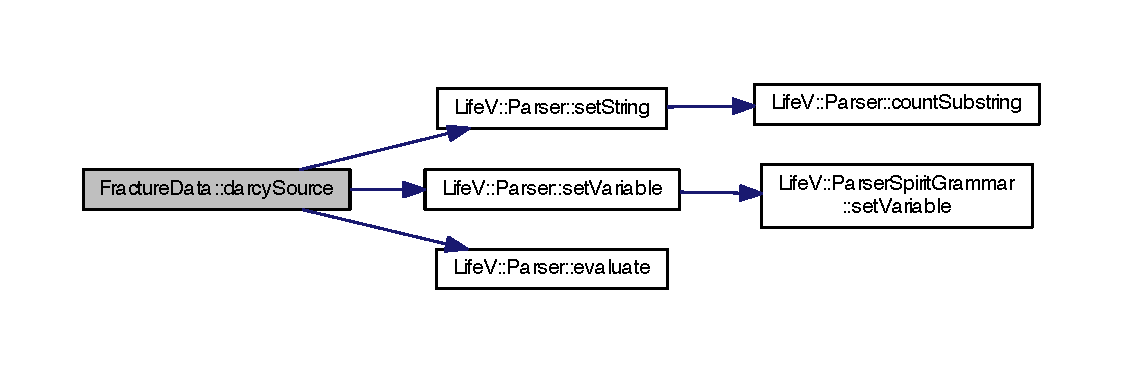
\includegraphics[width=350pt]{classFractureData_a8f935d962ae1bd93ca3e3b0955517db5_cgraph}
\end{center}
\end{figure}


\hypertarget{classFractureData_a0aaeeb3d9eedd46175759cd6b9536484}{\index{Fracture\-Data@{Fracture\-Data}!eta\-Normal\-Distribution@{eta\-Normal\-Distribution}}
\index{eta\-Normal\-Distribution@{eta\-Normal\-Distribution}!FractureData@{Fracture\-Data}}
\subsubsection[{eta\-Normal\-Distribution}]{\setlength{\rightskip}{0pt plus 5cm}scalar\-\_\-type Fracture\-Data\-::eta\-Normal\-Distribution (
\begin{DoxyParamCaption}
\item[{const base\-\_\-node \&}]{x}
\end{DoxyParamCaption}
)}}\label{classFractureData_a0aaeeb3d9eedd46175759cd6b9536484}


Funzione che restituisce un'eventuale modulazione del coefficiente di permeabilità in direzione normale. 


\begin{DoxyCode}
50 \{
51     M\_parser.\hyperlink{classLifeV_1_1Parser_ac05769e836a0dc95d9c020df361a5194}{setString} ( M\_etaNormalDistribution );
52     M\_parser.\hyperlink{classLifeV_1_1Parser_aa2b362e12b8feb60231705d499c9fbae}{setVariable} ( \textcolor{stringliteral}{"x"}, x [ 0 ] );
53     
54     \textcolor{keywordflow}{return} M\_parser.\hyperlink{classLifeV_1_1Parser_a51d84fd4ae6d420620e7beee58fad673}{evaluate} ();
55 \}\textcolor{comment}{// etaNormalDistribution}
\end{DoxyCode}


Questo è il grafo delle chiamate per questa funzione\-:\nopagebreak
\begin{figure}[H]
\begin{center}
\leavevmode
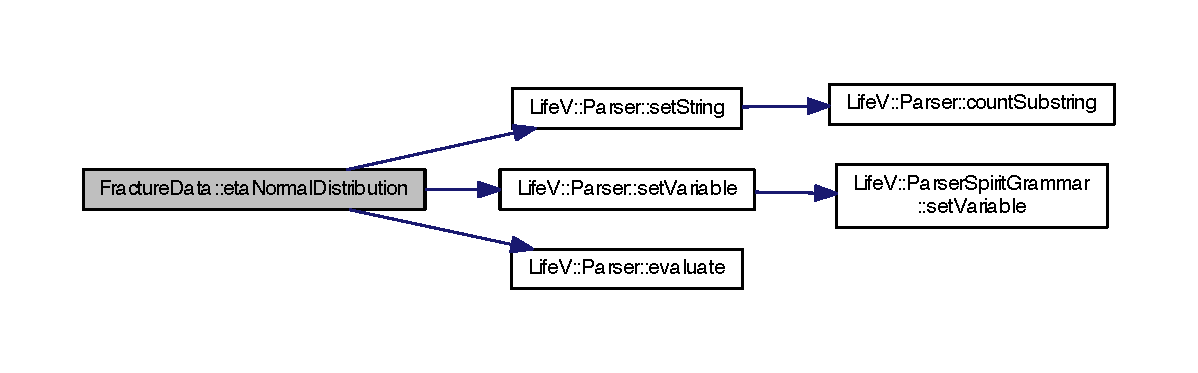
\includegraphics[width=350pt]{classFractureData_a0aaeeb3d9eedd46175759cd6b9536484_cgraph}
\end{center}
\end{figure}




Questo è il grafo dei chiamanti di questa funzione\-:\nopagebreak
\begin{figure}[H]
\begin{center}
\leavevmode
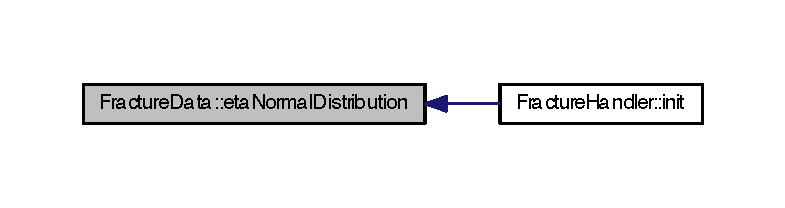
\includegraphics[width=350pt]{classFractureData_a0aaeeb3d9eedd46175759cd6b9536484_icgraph}
\end{center}
\end{figure}


\hypertarget{classFractureData_a0f989b64832a1f0fc77632c6803f102c}{\index{Fracture\-Data@{Fracture\-Data}!eta\-Tangential\-Distribution@{eta\-Tangential\-Distribution}}
\index{eta\-Tangential\-Distribution@{eta\-Tangential\-Distribution}!FractureData@{Fracture\-Data}}
\subsubsection[{eta\-Tangential\-Distribution}]{\setlength{\rightskip}{0pt plus 5cm}scalar\-\_\-type Fracture\-Data\-::eta\-Tangential\-Distribution (
\begin{DoxyParamCaption}
\item[{const base\-\_\-node \&}]{x}
\end{DoxyParamCaption}
)}}\label{classFractureData_a0f989b64832a1f0fc77632c6803f102c}


Funzione che restituisce un'eventuale modulazione del coefficiente di permeabilità in direzione tangenziale. 


\begin{DoxyCode}
59 \{
60     M\_parser.\hyperlink{classLifeV_1_1Parser_ac05769e836a0dc95d9c020df361a5194}{setString} ( M\_etaTangentialDistribution );
61     M\_parser.\hyperlink{classLifeV_1_1Parser_aa2b362e12b8feb60231705d499c9fbae}{setVariable} ( \textcolor{stringliteral}{"x"}, x [ 0 ] );
62     
63     \textcolor{keywordflow}{return} M\_parser.\hyperlink{classLifeV_1_1Parser_a51d84fd4ae6d420620e7beee58fad673}{evaluate} ();
64 \}\textcolor{comment}{// etaTangentialDistribution}
\end{DoxyCode}


Questo è il grafo delle chiamate per questa funzione\-:\nopagebreak
\begin{figure}[H]
\begin{center}
\leavevmode
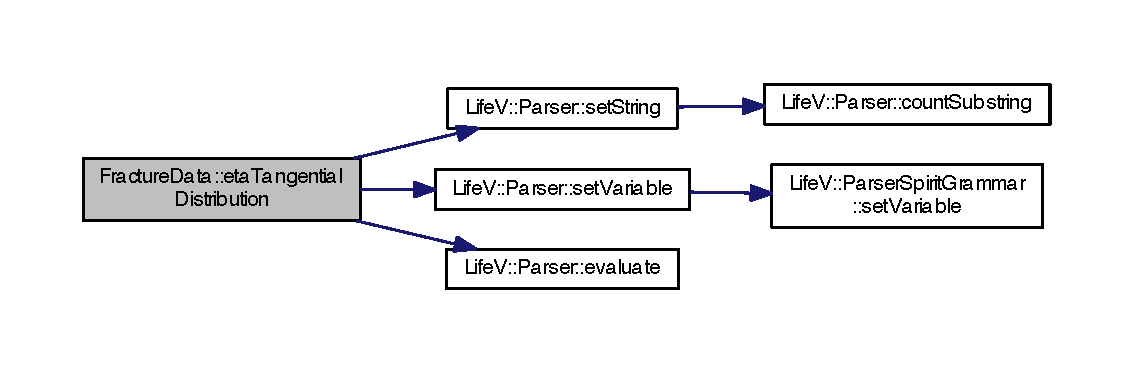
\includegraphics[width=350pt]{classFractureData_a0f989b64832a1f0fc77632c6803f102c_cgraph}
\end{center}
\end{figure}




Questo è il grafo dei chiamanti di questa funzione\-:\nopagebreak
\begin{figure}[H]
\begin{center}
\leavevmode
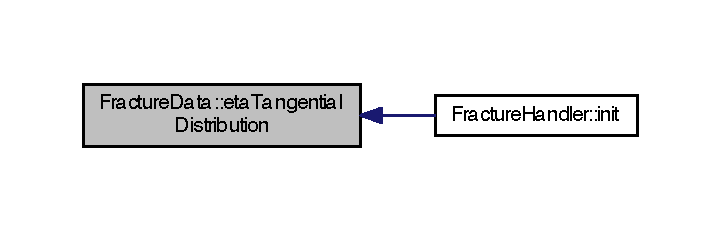
\includegraphics[width=346pt]{classFractureData_a0f989b64832a1f0fc77632c6803f102c_icgraph}
\end{center}
\end{figure}


\hypertarget{classFractureData_a7b75512224a34953960a9bd09f1af661}{\index{Fracture\-Data@{Fracture\-Data}!get\-Csi0@{get\-Csi0}}
\index{get\-Csi0@{get\-Csi0}!FractureData@{Fracture\-Data}}
\subsubsection[{get\-Csi0}]{\setlength{\rightskip}{0pt plus 5cm}scalar\-\_\-type Fracture\-Data\-::get\-Csi0 (
\begin{DoxyParamCaption}
{}
\end{DoxyParamCaption}
) const\hspace{0.3cm}{\ttfamily [inline]}}}\label{classFractureData_a7b75512224a34953960a9bd09f1af661}

\begin{DoxyCode}
69     \{
70         \textcolor{keywordflow}{return} M\_csi0;
71     \}
\end{DoxyCode}
\hypertarget{classFractureData_a9acc76c77282d4b5d0cdca18c2b1b9ea}{\index{Fracture\-Data@{Fracture\-Data}!get\-Eta\-Normal@{get\-Eta\-Normal}}
\index{get\-Eta\-Normal@{get\-Eta\-Normal}!FractureData@{Fracture\-Data}}
\subsubsection[{get\-Eta\-Normal}]{\setlength{\rightskip}{0pt plus 5cm}scalar\-\_\-type Fracture\-Data\-::get\-Eta\-Normal (
\begin{DoxyParamCaption}
{}
\end{DoxyParamCaption}
) const\hspace{0.3cm}{\ttfamily [inline]}}}\label{classFractureData_a9acc76c77282d4b5d0cdca18c2b1b9ea}

\begin{DoxyCode}
57     \{
58         \textcolor{keywordflow}{return} M\_etaNormal;
59     \}
\end{DoxyCode}


Questo è il grafo dei chiamanti di questa funzione\-:\nopagebreak
\begin{figure}[H]
\begin{center}
\leavevmode
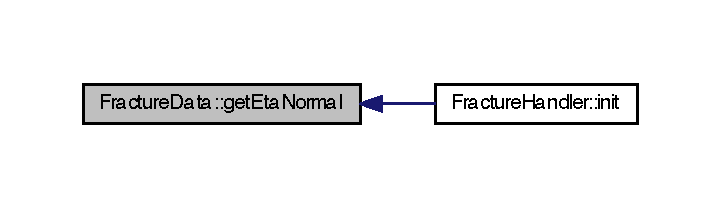
\includegraphics[width=346pt]{classFractureData_a9acc76c77282d4b5d0cdca18c2b1b9ea_icgraph}
\end{center}
\end{figure}


\hypertarget{classFractureData_a7378053b4009825b4a2957484cb2a5e8}{\index{Fracture\-Data@{Fracture\-Data}!get\-Eta\-Tangential@{get\-Eta\-Tangential}}
\index{get\-Eta\-Tangential@{get\-Eta\-Tangential}!FractureData@{Fracture\-Data}}
\subsubsection[{get\-Eta\-Tangential}]{\setlength{\rightskip}{0pt plus 5cm}scalar\-\_\-type Fracture\-Data\-::get\-Eta\-Tangential (
\begin{DoxyParamCaption}
{}
\end{DoxyParamCaption}
) const\hspace{0.3cm}{\ttfamily [inline]}}}\label{classFractureData_a7378053b4009825b4a2957484cb2a5e8}

\begin{DoxyCode}
63     \{
64         \textcolor{keywordflow}{return} M\_etaTangential;
65     \}
\end{DoxyCode}


Questo è il grafo dei chiamanti di questa funzione\-:\nopagebreak
\begin{figure}[H]
\begin{center}
\leavevmode
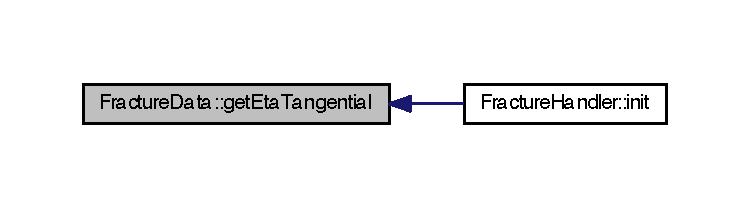
\includegraphics[width=350pt]{classFractureData_a7378053b4009825b4a2957484cb2a5e8_icgraph}
\end{center}
\end{figure}


\hypertarget{classFractureData_a606c22e054fdb5f8602ce39fa6ae15cc}{\index{Fracture\-Data@{Fracture\-Data}!get\-F\-E\-M\-Type\-Linear@{get\-F\-E\-M\-Type\-Linear}}
\index{get\-F\-E\-M\-Type\-Linear@{get\-F\-E\-M\-Type\-Linear}!FractureData@{Fracture\-Data}}
\subsubsection[{get\-F\-E\-M\-Type\-Linear}]{\setlength{\rightskip}{0pt plus 5cm}std\-::string Fracture\-Data\-::get\-F\-E\-M\-Type\-Linear (
\begin{DoxyParamCaption}
{}
\end{DoxyParamCaption}
) const\hspace{0.3cm}{\ttfamily [inline]}}}\label{classFractureData_a606c22e054fdb5f8602ce39fa6ae15cc}

\begin{DoxyCode}
141     \{
142         \textcolor{keywordflow}{return} M\_fEMTypeLinear;
143     \}
\end{DoxyCode}


Questo è il grafo dei chiamanti di questa funzione\-:\nopagebreak
\begin{figure}[H]
\begin{center}
\leavevmode
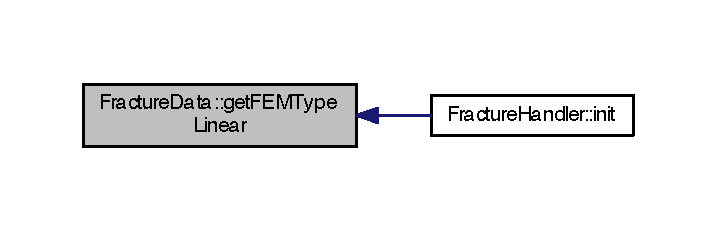
\includegraphics[width=344pt]{classFractureData_a606c22e054fdb5f8602ce39fa6ae15cc_icgraph}
\end{center}
\end{figure}


\hypertarget{classFractureData_a643b9a8a33405ec7aaa6b5612cb81d57}{\index{Fracture\-Data@{Fracture\-Data}!get\-F\-E\-M\-Type\-Pressure@{get\-F\-E\-M\-Type\-Pressure}}
\index{get\-F\-E\-M\-Type\-Pressure@{get\-F\-E\-M\-Type\-Pressure}!FractureData@{Fracture\-Data}}
\subsubsection[{get\-F\-E\-M\-Type\-Pressure}]{\setlength{\rightskip}{0pt plus 5cm}std\-::string Fracture\-Data\-::get\-F\-E\-M\-Type\-Pressure (
\begin{DoxyParamCaption}
{}
\end{DoxyParamCaption}
) const\hspace{0.3cm}{\ttfamily [inline]}}}\label{classFractureData_a643b9a8a33405ec7aaa6b5612cb81d57}

\begin{DoxyCode}
129     \{
130         \textcolor{keywordflow}{return} M\_fEMTypePressure;
131     \}
\end{DoxyCode}


Questo è il grafo dei chiamanti di questa funzione\-:\nopagebreak
\begin{figure}[H]
\begin{center}
\leavevmode
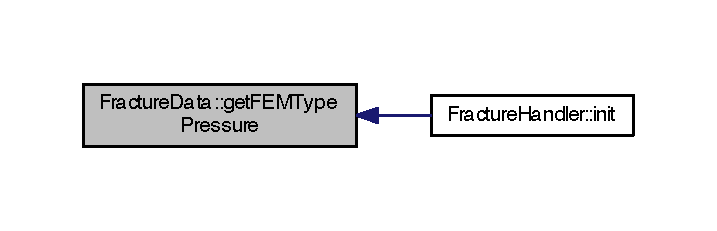
\includegraphics[width=344pt]{classFractureData_a643b9a8a33405ec7aaa6b5612cb81d57_icgraph}
\end{center}
\end{figure}


\hypertarget{classFractureData_a7396b67399a1ae8e5550841907c0dcb5}{\index{Fracture\-Data@{Fracture\-Data}!get\-F\-E\-M\-Type\-Velocity@{get\-F\-E\-M\-Type\-Velocity}}
\index{get\-F\-E\-M\-Type\-Velocity@{get\-F\-E\-M\-Type\-Velocity}!FractureData@{Fracture\-Data}}
\subsubsection[{get\-F\-E\-M\-Type\-Velocity}]{\setlength{\rightskip}{0pt plus 5cm}std\-::string Fracture\-Data\-::get\-F\-E\-M\-Type\-Velocity (
\begin{DoxyParamCaption}
{}
\end{DoxyParamCaption}
) const\hspace{0.3cm}{\ttfamily [inline]}}}\label{classFractureData_a7396b67399a1ae8e5550841907c0dcb5}

\begin{DoxyCode}
135     \{
136         \textcolor{keywordflow}{return} M\_fEMTypeVelocity;
137     \}
\end{DoxyCode}


Questo è il grafo dei chiamanti di questa funzione\-:\nopagebreak
\begin{figure}[H]
\begin{center}
\leavevmode
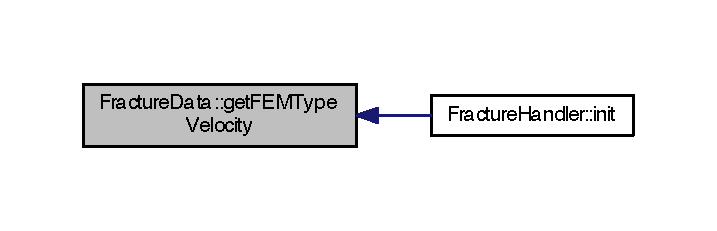
\includegraphics[width=344pt]{classFractureData_a7396b67399a1ae8e5550841907c0dcb5_icgraph}
\end{center}
\end{figure}


\hypertarget{classFractureData_a9333d8e89dc92023d97a48c1905ada76}{\index{Fracture\-Data@{Fracture\-Data}!get\-Integration\-Type\-Pressure@{get\-Integration\-Type\-Pressure}}
\index{get\-Integration\-Type\-Pressure@{get\-Integration\-Type\-Pressure}!FractureData@{Fracture\-Data}}
\subsubsection[{get\-Integration\-Type\-Pressure}]{\setlength{\rightskip}{0pt plus 5cm}std\-::string Fracture\-Data\-::get\-Integration\-Type\-Pressure (
\begin{DoxyParamCaption}
{}
\end{DoxyParamCaption}
) const\hspace{0.3cm}{\ttfamily [inline]}}}\label{classFractureData_a9333d8e89dc92023d97a48c1905ada76}

\begin{DoxyCode}
117     \{
118         \textcolor{keywordflow}{return} M\_integrationTypePressure;
119     \}
\end{DoxyCode}


Questo è il grafo dei chiamanti di questa funzione\-:\nopagebreak
\begin{figure}[H]
\begin{center}
\leavevmode
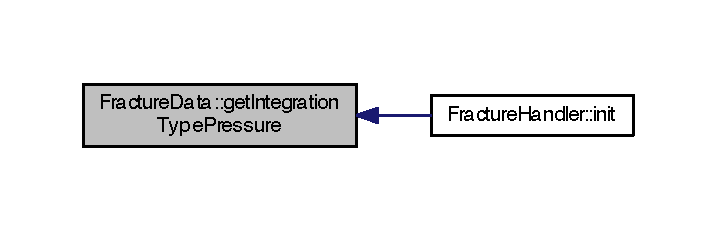
\includegraphics[width=344pt]{classFractureData_a9333d8e89dc92023d97a48c1905ada76_icgraph}
\end{center}
\end{figure}


\hypertarget{classFractureData_a8a8a198482de6bf4104746bc1d0510c6}{\index{Fracture\-Data@{Fracture\-Data}!get\-Integration\-Type\-Velocity@{get\-Integration\-Type\-Velocity}}
\index{get\-Integration\-Type\-Velocity@{get\-Integration\-Type\-Velocity}!FractureData@{Fracture\-Data}}
\subsubsection[{get\-Integration\-Type\-Velocity}]{\setlength{\rightskip}{0pt plus 5cm}std\-::string Fracture\-Data\-::get\-Integration\-Type\-Velocity (
\begin{DoxyParamCaption}
{}
\end{DoxyParamCaption}
) const\hspace{0.3cm}{\ttfamily [inline]}}}\label{classFractureData_a8a8a198482de6bf4104746bc1d0510c6}

\begin{DoxyCode}
111     \{
112         \textcolor{keywordflow}{return} M\_integrationTypeVelocity;
113     \}
\end{DoxyCode}


Questo è il grafo dei chiamanti di questa funzione\-:\nopagebreak
\begin{figure}[H]
\begin{center}
\leavevmode
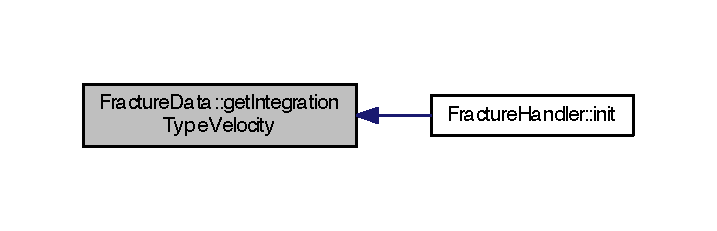
\includegraphics[width=344pt]{classFractureData_a8a8a198482de6bf4104746bc1d0510c6_icgraph}
\end{center}
\end{figure}


\hypertarget{classFractureData_abaebcf16d83713858e25837939ad3161}{\index{Fracture\-Data@{Fracture\-Data}!get\-Length\-Abscissa@{get\-Length\-Abscissa}}
\index{get\-Length\-Abscissa@{get\-Length\-Abscissa}!FractureData@{Fracture\-Data}}
\subsubsection[{get\-Length\-Abscissa}]{\setlength{\rightskip}{0pt plus 5cm}scalar\-\_\-type Fracture\-Data\-::get\-Length\-Abscissa (
\begin{DoxyParamCaption}
{}
\end{DoxyParamCaption}
) const\hspace{0.3cm}{\ttfamily [inline]}}}\label{classFractureData_abaebcf16d83713858e25837939ad3161}

\begin{DoxyCode}
75     \{
76         \textcolor{keywordflow}{return} M\_lengthAbscissa;
77     \}
\end{DoxyCode}


Questo è il grafo dei chiamanti di questa funzione\-:\nopagebreak
\begin{figure}[H]
\begin{center}
\leavevmode
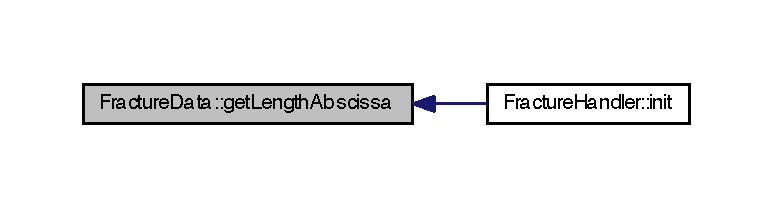
\includegraphics[width=350pt]{classFractureData_abaebcf16d83713858e25837939ad3161_icgraph}
\end{center}
\end{figure}


\hypertarget{classFractureData_a905e953f685b1329ddcc7ee56f8302b1}{\index{Fracture\-Data@{Fracture\-Data}!get\-Length\-Ordinate@{get\-Length\-Ordinate}}
\index{get\-Length\-Ordinate@{get\-Length\-Ordinate}!FractureData@{Fracture\-Data}}
\subsubsection[{get\-Length\-Ordinate}]{\setlength{\rightskip}{0pt plus 5cm}scalar\-\_\-type Fracture\-Data\-::get\-Length\-Ordinate (
\begin{DoxyParamCaption}
{}
\end{DoxyParamCaption}
) const\hspace{0.3cm}{\ttfamily [inline]}}}\label{classFractureData_a905e953f685b1329ddcc7ee56f8302b1}

\begin{DoxyCode}
81     \{
82         \textcolor{keywordflow}{return} M\_lengthOrdinate;
83     \}
\end{DoxyCode}


Questo è il grafo dei chiamanti di questa funzione\-:\nopagebreak
\begin{figure}[H]
\begin{center}
\leavevmode
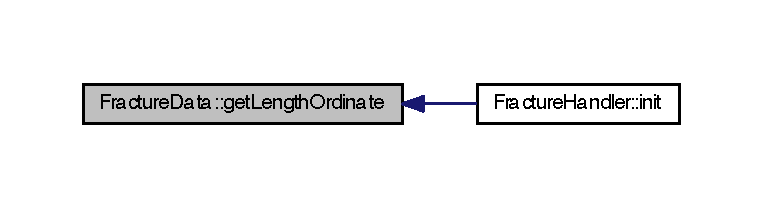
\includegraphics[width=350pt]{classFractureData_a905e953f685b1329ddcc7ee56f8302b1_icgraph}
\end{center}
\end{figure}


\hypertarget{classFractureData_a79747fff53da9d858950d83ad0114288}{\index{Fracture\-Data@{Fracture\-Data}!get\-Length\-Quota@{get\-Length\-Quota}}
\index{get\-Length\-Quota@{get\-Length\-Quota}!FractureData@{Fracture\-Data}}
\subsubsection[{get\-Length\-Quota}]{\setlength{\rightskip}{0pt plus 5cm}scalar\-\_\-type Fracture\-Data\-::get\-Length\-Quota (
\begin{DoxyParamCaption}
{}
\end{DoxyParamCaption}
) const\hspace{0.3cm}{\ttfamily [inline]}}}\label{classFractureData_a79747fff53da9d858950d83ad0114288}

\begin{DoxyCode}
87     \{
88         \textcolor{keywordflow}{return} M\_lengthQuota;
89     \}
\end{DoxyCode}


Questo è il grafo dei chiamanti di questa funzione\-:\nopagebreak
\begin{figure}[H]
\begin{center}
\leavevmode
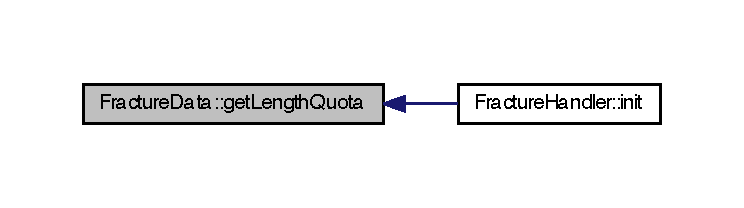
\includegraphics[width=350pt]{classFractureData_a79747fff53da9d858950d83ad0114288_icgraph}
\end{center}
\end{figure}


\hypertarget{classFractureData_aaded6c0452470489beb4ab95b5f4158f}{\index{Fracture\-Data@{Fracture\-Data}!get\-Mesh\-Type@{get\-Mesh\-Type}}
\index{get\-Mesh\-Type@{get\-Mesh\-Type}!FractureData@{Fracture\-Data}}
\subsubsection[{get\-Mesh\-Type}]{\setlength{\rightskip}{0pt plus 5cm}std\-::string Fracture\-Data\-::get\-Mesh\-Type (
\begin{DoxyParamCaption}
{}
\end{DoxyParamCaption}
) const\hspace{0.3cm}{\ttfamily [inline]}}}\label{classFractureData_aaded6c0452470489beb4ab95b5f4158f}

\begin{DoxyCode}
123     \{
124         \textcolor{keywordflow}{return} M\_meshType;
125     \}
\end{DoxyCode}


Questo è il grafo dei chiamanti di questa funzione\-:\nopagebreak
\begin{figure}[H]
\begin{center}
\leavevmode
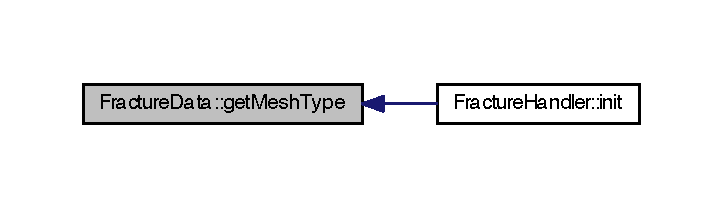
\includegraphics[width=347pt]{classFractureData_aaded6c0452470489beb4ab95b5f4158f_icgraph}
\end{center}
\end{figure}


\hypertarget{classFractureData_a4ead03266295fe14fa3285692f945d89}{\index{Fracture\-Data@{Fracture\-Data}!get\-Space\-Dimension@{get\-Space\-Dimension}}
\index{get\-Space\-Dimension@{get\-Space\-Dimension}!FractureData@{Fracture\-Data}}
\subsubsection[{get\-Space\-Dimension}]{\setlength{\rightskip}{0pt plus 5cm}bgeot\-::dim\-\_\-type Fracture\-Data\-::get\-Space\-Dimension (
\begin{DoxyParamCaption}
{}
\end{DoxyParamCaption}
) const\hspace{0.3cm}{\ttfamily [inline]}}}\label{classFractureData_a4ead03266295fe14fa3285692f945d89}

\begin{DoxyCode}
105     \{
106         \textcolor{keywordflow}{return} M\_spaceDimension;
107     \}
\end{DoxyCode}


Questo è il grafo dei chiamanti di questa funzione\-:\nopagebreak
\begin{figure}[H]
\begin{center}
\leavevmode
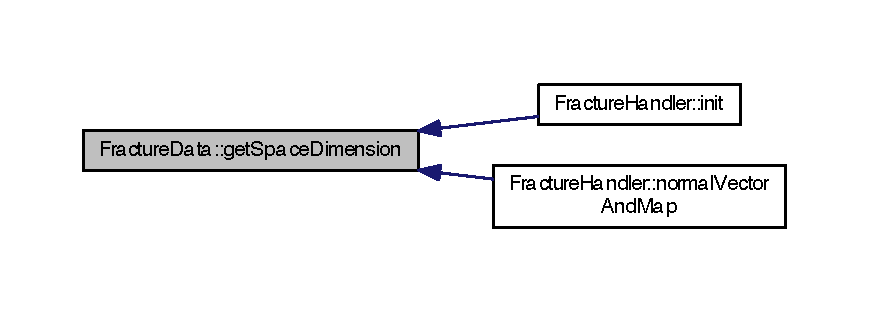
\includegraphics[width=350pt]{classFractureData_a4ead03266295fe14fa3285692f945d89_icgraph}
\end{center}
\end{figure}


\hypertarget{classFractureData_a5c10d579be7849be1a126c24982f8a23}{\index{Fracture\-Data@{Fracture\-Data}!get\-Spatial\-Discretization@{get\-Spatial\-Discretization}}
\index{get\-Spatial\-Discretization@{get\-Spatial\-Discretization}!FractureData@{Fracture\-Data}}
\subsubsection[{get\-Spatial\-Discretization}]{\setlength{\rightskip}{0pt plus 5cm}size\-\_\-type Fracture\-Data\-::get\-Spatial\-Discretization (
\begin{DoxyParamCaption}
{}
\end{DoxyParamCaption}
) const\hspace{0.3cm}{\ttfamily [inline]}}}\label{classFractureData_a5c10d579be7849be1a126c24982f8a23}

\begin{DoxyCode}
93     \{
94         \textcolor{keywordflow}{return} M\_spatialDiscretization;
95     \}
\end{DoxyCode}


Questo è il grafo dei chiamanti di questa funzione\-:\nopagebreak
\begin{figure}[H]
\begin{center}
\leavevmode
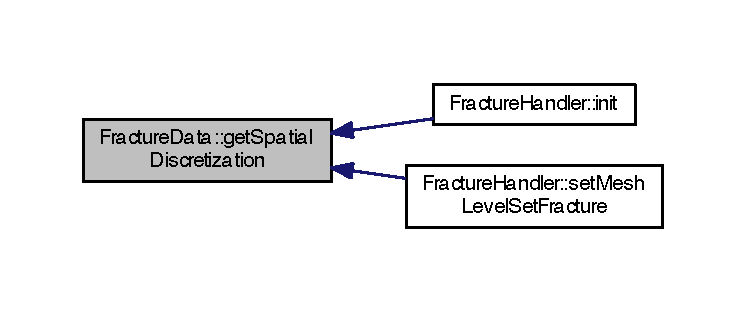
\includegraphics[width=350pt]{classFractureData_a5c10d579be7849be1a126c24982f8a23_icgraph}
\end{center}
\end{figure}


\hypertarget{classFractureData_a3ecc0d132f9cc105af6b24d676a7b9c5}{\index{Fracture\-Data@{Fracture\-Data}!get\-Thickness@{get\-Thickness}}
\index{get\-Thickness@{get\-Thickness}!FractureData@{Fracture\-Data}}
\subsubsection[{get\-Thickness}]{\setlength{\rightskip}{0pt plus 5cm}scalar\-\_\-type Fracture\-Data\-::get\-Thickness (
\begin{DoxyParamCaption}
{}
\end{DoxyParamCaption}
) const\hspace{0.3cm}{\ttfamily [inline]}}}\label{classFractureData_a3ecc0d132f9cc105af6b24d676a7b9c5}

\begin{DoxyCode}
51     \{
52         \textcolor{keywordflow}{return} M\_thickness;
53     \}
\end{DoxyCode}
\hypertarget{classFractureData_a485e084e083d9181750f19db6842a5e0}{\index{Fracture\-Data@{Fracture\-Data}!get\-Translate\-Abscissa@{get\-Translate\-Abscissa}}
\index{get\-Translate\-Abscissa@{get\-Translate\-Abscissa}!FractureData@{Fracture\-Data}}
\subsubsection[{get\-Translate\-Abscissa}]{\setlength{\rightskip}{0pt plus 5cm}scalar\-\_\-type Fracture\-Data\-::get\-Translate\-Abscissa (
\begin{DoxyParamCaption}
{}
\end{DoxyParamCaption}
) const\hspace{0.3cm}{\ttfamily [inline]}}}\label{classFractureData_a485e084e083d9181750f19db6842a5e0}

\begin{DoxyCode}
99     \{
100         \textcolor{keywordflow}{return} M\_translateAbscissa;
101     \}
\end{DoxyCode}
\hypertarget{classFractureData_ab79d66dd830b6e1c55ade0d940c5c8cf}{\index{Fracture\-Data@{Fracture\-Data}!mesh\-Spacing@{mesh\-Spacing}}
\index{mesh\-Spacing@{mesh\-Spacing}!FractureData@{Fracture\-Data}}
\subsubsection[{mesh\-Spacing}]{\setlength{\rightskip}{0pt plus 5cm}scalar\-\_\-type Fracture\-Data\-::mesh\-Spacing (
\begin{DoxyParamCaption}
\item[{const scalar\-\_\-type \&}]{x}
\end{DoxyParamCaption}
)}}\label{classFractureData_ab79d66dd830b6e1c55ade0d940c5c8cf}

\begin{DoxyCode}
99 \{
100     M\_parser.\hyperlink{classLifeV_1_1Parser_ac05769e836a0dc95d9c020df361a5194}{setString} ( M\_meshSpacing );
101     M\_parser.\hyperlink{classLifeV_1_1Parser_aa2b362e12b8feb60231705d499c9fbae}{setVariable} ( \textcolor{stringliteral}{"x"}, x );
102     
103     \textcolor{keywordflow}{return} M\_parser.\hyperlink{classLifeV_1_1Parser_a51d84fd4ae6d420620e7beee58fad673}{evaluate} ();
104 \}\textcolor{comment}{// meshSpacing}
\end{DoxyCode}


Questo è il grafo delle chiamate per questa funzione\-:\nopagebreak
\begin{figure}[H]
\begin{center}
\leavevmode
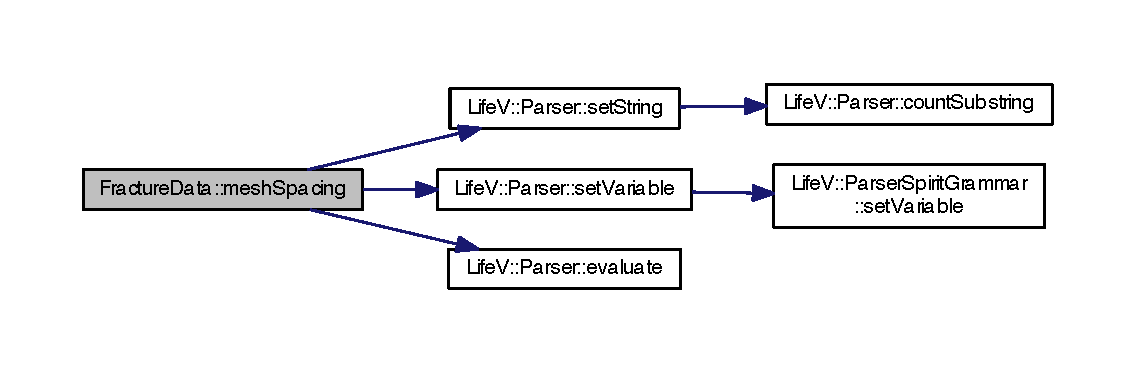
\includegraphics[width=350pt]{classFractureData_ab79d66dd830b6e1c55ade0d940c5c8cf_cgraph}
\end{center}
\end{figure}




Questo è il grafo dei chiamanti di questa funzione\-:\nopagebreak
\begin{figure}[H]
\begin{center}
\leavevmode
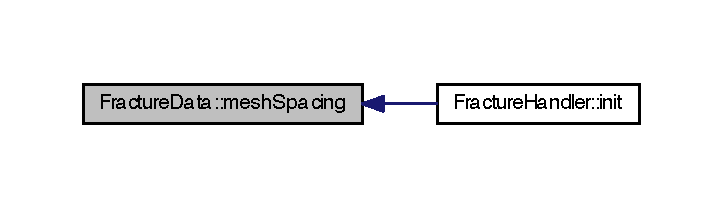
\includegraphics[width=347pt]{classFractureData_ab79d66dd830b6e1c55ade0d940c5c8cf_icgraph}
\end{center}
\end{figure}


\hypertarget{classFractureData_aa90769a75aff6485824ecd2090c8b4ee}{\index{Fracture\-Data@{Fracture\-Data}!pressure\-Exact@{pressure\-Exact}}
\index{pressure\-Exact@{pressure\-Exact}!FractureData@{Fracture\-Data}}
\subsubsection[{pressure\-Exact}]{\setlength{\rightskip}{0pt plus 5cm}scalar\-\_\-type Fracture\-Data\-::pressure\-Exact (
\begin{DoxyParamCaption}
\item[{const base\-\_\-node \&}]{x}
\end{DoxyParamCaption}
)}}\label{classFractureData_aa90769a75aff6485824ecd2090c8b4ee}

\begin{DoxyCode}
90 \{
91     M\_parser.\hyperlink{classLifeV_1_1Parser_ac05769e836a0dc95d9c020df361a5194}{setString} ( M\_pressureExact );
92     M\_parser.\hyperlink{classLifeV_1_1Parser_aa2b362e12b8feb60231705d499c9fbae}{setVariable} ( \textcolor{stringliteral}{"x"}, x [ 0 ] );
93     
94     \textcolor{keywordflow}{return} M\_parser.\hyperlink{classLifeV_1_1Parser_a51d84fd4ae6d420620e7beee58fad673}{evaluate} ();
95 \}\textcolor{comment}{// pressureExact}
\end{DoxyCode}


Questo è il grafo delle chiamate per questa funzione\-:\nopagebreak
\begin{figure}[H]
\begin{center}
\leavevmode
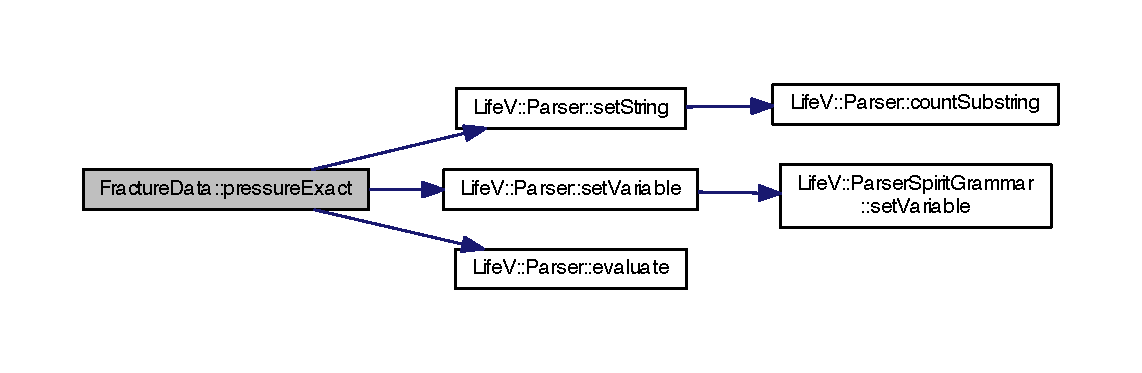
\includegraphics[width=350pt]{classFractureData_aa90769a75aff6485824ecd2090c8b4ee_cgraph}
\end{center}
\end{figure}


\hypertarget{classFractureData_a8342142df05ded99f3a6c8d39dbfdc0e}{\index{Fracture\-Data@{Fracture\-Data}!velocity\-Exact@{velocity\-Exact}}
\index{velocity\-Exact@{velocity\-Exact}!FractureData@{Fracture\-Data}}
\subsubsection[{velocity\-Exact}]{\setlength{\rightskip}{0pt plus 5cm}scalar\-\_\-type Fracture\-Data\-::velocity\-Exact (
\begin{DoxyParamCaption}
\item[{const base\-\_\-node \&}]{x, }
\item[{const base\-\_\-node \&}]{n}
\end{DoxyParamCaption}
)}}\label{classFractureData_a8342142df05ded99f3a6c8d39dbfdc0e}

\begin{DoxyCode}
69 \{
70     M\_parser.\hyperlink{classLifeV_1_1Parser_ac05769e836a0dc95d9c020df361a5194}{setString} ( M\_velocityExact );
71     M\_parser.\hyperlink{classLifeV_1_1Parser_aa2b362e12b8feb60231705d499c9fbae}{setVariable} ( \textcolor{stringliteral}{"x"}, x [ 0 ] );
72     M\_parser.\hyperlink{classLifeV_1_1Parser_aa2b362e12b8feb60231705d499c9fbae}{setVariable} ( \textcolor{stringliteral}{"y"}, x [ 1 ] );
73     M\_parser.\hyperlink{classLifeV_1_1Parser_aa2b362e12b8feb60231705d499c9fbae}{setVariable} ( \textcolor{stringliteral}{"n1"}, n [ 0 ] );
74     M\_parser.\hyperlink{classLifeV_1_1Parser_aa2b362e12b8feb60231705d499c9fbae}{setVariable} ( \textcolor{stringliteral}{"n2"}, n [ 1 ] );
75     
76     \textcolor{keywordflow}{return} M\_parser.\hyperlink{classLifeV_1_1Parser_a51d84fd4ae6d420620e7beee58fad673}{evaluate} ();
77 \}\textcolor{comment}{// velocityExact}
\end{DoxyCode}


Questo è il grafo delle chiamate per questa funzione\-:\nopagebreak
\begin{figure}[H]
\begin{center}
\leavevmode
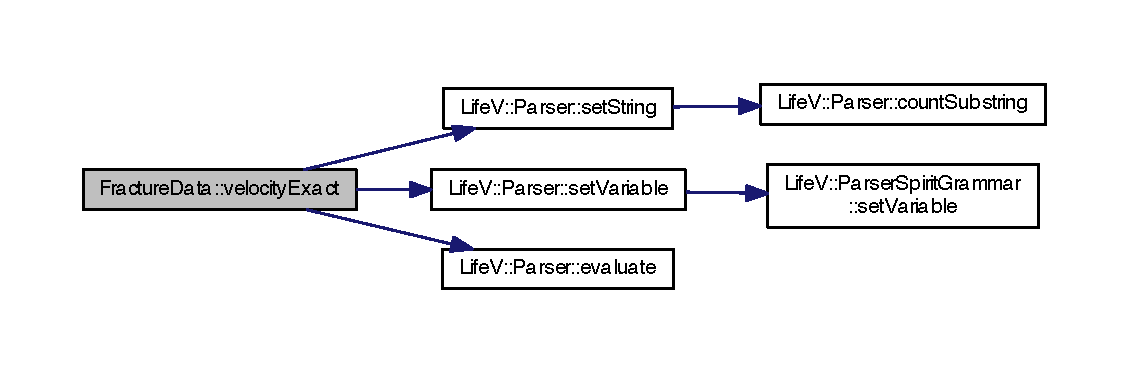
\includegraphics[width=350pt]{classFractureData_a8342142df05ded99f3a6c8d39dbfdc0e_cgraph}
\end{center}
\end{figure}




La documentazione per questa classe è stata generata a partire dai seguenti file\-:\begin{DoxyCompactItemize}
\item 
include/\hyperlink{FractureData_8h}{Fracture\-Data.\-h}\item 
src/\hyperlink{FractureData_8cc}{Fracture\-Data.\-cc}\end{DoxyCompactItemize}

\hypertarget{classFractureEnd}{\section{Riferimenti per la classe Fracture\-End}
\label{classFractureEnd}\index{Fracture\-End@{Fracture\-End}}
}


\hyperlink{TriangleHandler_8h}{Triangle\-Handler.\-h}.  




{\ttfamily \#include $<$Triangle\-Handler.\-h$>$}

\subsection*{Membri pubblici}
\begin{DoxyCompactItemize}
\item 
\hyperlink{classFractureEnd_a5be0d3eb231ecbc491fb9c07bbe44183}{Fracture\-End} (\hyperlink{classPointData}{Point\-Data} \&, scalar\-\_\-type)
\item 
\hyperlink{classPointData}{Point\-Data} \hyperlink{classFractureEnd_a48187852ce2e959d00577fe4d66c2e0f}{get\-Point} () const 
\item 
scalar\-\_\-type \hyperlink{classFractureEnd_a2b70172b4593324288f5779b7998d4a3}{get\-Thickness} () const 
\item 
\hyperlink{classFractureEnd}{Fracture\-End} \& \hyperlink{classFractureEnd_a94df97c8e4f3e68a62ebaa3ae754106f}{operator=} (const \hyperlink{classFractureEnd}{Fracture\-End} \&t)
\end{DoxyCompactItemize}


\subsection{Descrizione dettagliata}
\hyperlink{TriangleHandler_8h}{Triangle\-Handler.\-h}. 

Classe che costruisce il triangolo 2d dell'intersezione Classe che rappresenta la fine di una frattura 

\subsection{Documentazione dei costruttori e dei distruttori}
\hypertarget{classFractureEnd_a5be0d3eb231ecbc491fb9c07bbe44183}{\index{Fracture\-End@{Fracture\-End}!Fracture\-End@{Fracture\-End}}
\index{Fracture\-End@{Fracture\-End}!FractureEnd@{Fracture\-End}}
\subsubsection[{Fracture\-End}]{\setlength{\rightskip}{0pt plus 5cm}Fracture\-End\-::\-Fracture\-End (
\begin{DoxyParamCaption}
\item[{{\bf Point\-Data} \&}]{a, }
\item[{scalar\-\_\-type}]{t}
\end{DoxyParamCaption}
)}}\label{classFractureEnd_a5be0d3eb231ecbc491fb9c07bbe44183}

\begin{DoxyCode}
5 \{
6     M\_endPoint = a;
7 
8     M\_thickness = t;
9 \}\textcolor{comment}{//costruttore FractureEnd}
\end{DoxyCode}


\subsection{Documentazione delle funzioni membro}
\hypertarget{classFractureEnd_a48187852ce2e959d00577fe4d66c2e0f}{\index{Fracture\-End@{Fracture\-End}!get\-Point@{get\-Point}}
\index{get\-Point@{get\-Point}!FractureEnd@{Fracture\-End}}
\subsubsection[{get\-Point}]{\setlength{\rightskip}{0pt plus 5cm}{\bf Point\-Data} Fracture\-End\-::get\-Point (
\begin{DoxyParamCaption}
{}
\end{DoxyParamCaption}
) const\hspace{0.3cm}{\ttfamily [inline]}}}\label{classFractureEnd_a48187852ce2e959d00577fe4d66c2e0f}

\begin{DoxyCode}
26         \{
27             \textcolor{keywordflow}{return} M\_endPoint;
28         \}
\end{DoxyCode}
\hypertarget{classFractureEnd_a2b70172b4593324288f5779b7998d4a3}{\index{Fracture\-End@{Fracture\-End}!get\-Thickness@{get\-Thickness}}
\index{get\-Thickness@{get\-Thickness}!FractureEnd@{Fracture\-End}}
\subsubsection[{get\-Thickness}]{\setlength{\rightskip}{0pt plus 5cm}scalar\-\_\-type Fracture\-End\-::get\-Thickness (
\begin{DoxyParamCaption}
{}
\end{DoxyParamCaption}
) const\hspace{0.3cm}{\ttfamily [inline]}}}\label{classFractureEnd_a2b70172b4593324288f5779b7998d4a3}

\begin{DoxyCode}
31         \{
32             \textcolor{keywordflow}{return} M\_thickness;
33         \}
\end{DoxyCode}
\hypertarget{classFractureEnd_a94df97c8e4f3e68a62ebaa3ae754106f}{\index{Fracture\-End@{Fracture\-End}!operator=@{operator=}}
\index{operator=@{operator=}!FractureEnd@{Fracture\-End}}
\subsubsection[{operator=}]{\setlength{\rightskip}{0pt plus 5cm}{\bf Fracture\-End}\& Fracture\-End\-::operator= (
\begin{DoxyParamCaption}
\item[{const {\bf Fracture\-End} \&}]{t}
\end{DoxyParamCaption}
)\hspace{0.3cm}{\ttfamily [inline]}}}\label{classFractureEnd_a94df97c8e4f3e68a62ebaa3ae754106f}

\begin{DoxyCode}
37         \{
38             \textcolor{keywordflow}{if} (\textcolor{keyword}{this} !=&t)
39             \{
40                 M\_endPoint = t.\hyperlink{classFractureEnd_a48187852ce2e959d00577fe4d66c2e0f}{getPoint}();
41                 M\_thickness = t.\hyperlink{classFractureEnd_a2b70172b4593324288f5779b7998d4a3}{getThickness}();
42             \}
43     
44             \textcolor{keywordflow}{return} *\textcolor{keyword}{this};
45         \}
\end{DoxyCode}


La documentazione per questa classe è stata generata a partire dai seguenti file\-:\begin{DoxyCompactItemize}
\item 
include/\hyperlink{TriangleHandler_8h}{Triangle\-Handler.\-h}\item 
src/\hyperlink{TriangleHandler_8cc}{Triangle\-Handler.\-cc}\end{DoxyCompactItemize}

\hypertarget{classFractureHandler}{\section{Riferimenti per la classe Fracture\-Handler}
\label{classFractureHandler}\index{Fracture\-Handler@{Fracture\-Handler}}
}


\hyperlink{FractureHandler_8h}{Fracture\-Handler.\-h}.  




{\ttfamily \#include $<$Fracture\-Handler.\-h$>$}

\subsection*{Tipi pubblici}
\begin{DoxyCompactItemize}
\item 
enum \{ \hyperlink{classFractureHandler_a495ad4fc72d0c47c8f0424842f1153aaaa992cc3ad024a030ecd798dc319c95ac}{F\-R\-A\-C\-T\-U\-R\-E\-\_\-\-U\-N\-C\-U\-T} = 10000, 
\hyperlink{classFractureHandler_a495ad4fc72d0c47c8f0424842f1153aaa781cae3f3b99bf9357fed2833d315537}{F\-R\-A\-C\-T\-U\-R\-E\-\_\-\-I\-N\-T\-E\-R\-S\-E\-C\-T} = 10000
 \}
\begin{DoxyCompactList}\small\item\em flags che uso per distinguere sulla mesh di ogni level set le regioni \char`\"{} non tagliate \char`\"{}, cioè dove non vi è intersezione con altre fratture, dalle regioni \char`\"{} tagliate \char`\"{}, cioè dove il level set ha un'intersezione \end{DoxyCompactList}\end{DoxyCompactItemize}
\subsection*{Membri pubblici}
\begin{DoxyCompactItemize}
\item 
\hyperlink{classFractureHandler_aa3872456d95550cdd424908bbb5a15ec}{Fracture\-Handler} (const Get\-Pot \&data\-File, const size\-\_\-type \&I\-D, const std\-::string \&section=\char`\"{}fracture\-Data/\char`\"{})
\begin{DoxyCompactList}\small\item\em \hyperlink{FractureHandler_8cc}{Fracture\-Handler.\-cc}. \end{DoxyCompactList}\item 
void \hyperlink{classFractureHandler_aa28ce054ba2a2679214956c71f8cf1e0}{init} ()
\begin{DoxyCompactList}\small\item\em funzione che inizializza la frattura Ogni frattura ha una rappresentazione 1d, ma la mesh reale è una mesh di punti 2d ( sono i punti del tipo (x,y) che stanno sulla curva y=f(x) ) e questo comporta dei problemi per l'integrazione. \end{DoxyCompactList}\item 
void \hyperlink{classFractureHandler_aec1fc4e2664b3fe60877b63024af3605}{normal\-Vector\-And\-Map} (const getfem\-::mesh\-\_\-fem \&medium\-Mesh\-F\-E\-M\-Pressure)
\begin{DoxyCompactList}\small\item\em funzione che calcola il vettore normale alla frattura e la mappa di conversione dalla mesh reale alla mesh piatta \end{DoxyCompactList}\item 
void \hyperlink{classFractureHandler_a87f0f8e2998b621b481173ec8d9aaa2a}{compute\-Inv\-H} (const \hyperlink{BCHandler_8h_aa175884cb453788647f17f2230a2a762}{B\-C\-Handler\-Ptr\-\_\-\-Type} \&bc\-Handler)
\begin{DoxyCompactList}\small\item\em funzione che calcola il passo di griglia, h$^\wedge$-\/1 \end{DoxyCompactList}\item 
const getfem\-::mesh \& \hyperlink{classFractureHandler_a9ff9f584b850d6b750981befdbefbdbe}{get\-Mesh\-Flat} () const 
\item 
getfem\-::mesh \& \hyperlink{classFractureHandler_ad9b02a825d444016b3ab8ee901f887f6}{get\-Mesh\-Flat} ()
\item 
const getfem\-::mesh\-\_\-fem \& \hyperlink{classFractureHandler_ae54c07023428b44556bbec4da5be9306}{get\-Mesh\-F\-E\-M\-Velocity} () const 
\item 
const getfem\-::mesh\-\_\-fem \& \hyperlink{classFractureHandler_a6dc20a9624f9dff49b1c58f0dd261002}{get\-Mesh\-F\-E\-M\-Pressure} () const 
\item 
const getfem\-::mesh\-\_\-im \& \hyperlink{classFractureHandler_afe4c174c17862ed30b99ebe4a80aa695}{get\-Integration\-Method\-Velocity} () const 
\item 
const getfem\-::mesh\-\_\-im \& \hyperlink{classFractureHandler_ad7afd53439c3067f46a0fb6e1473d661}{get\-Integration\-Method\-Pressure} () const 
\item 
\hyperlink{classFractureData}{Fracture\-Data} \& \hyperlink{classFractureHandler_a68ed77a8d9816a472700ee4bcf2f505d}{get\-Data} ()
\item 
\hyperlink{LevelSetHandler_8h_aba343569cb3213c103252f69c39cad0b}{Level\-Set\-Handler\-Ptr\-\_\-\-Type} \& \hyperlink{classFractureHandler_af37ab12a17f812a960da2aa71699ba0f}{get\-Level\-Set} ()
\item 
const \hyperlink{Core_8h_a4e75b5863535ba1dd79942de2846eff0}{scalar\-Vector\-\_\-\-Type} \& \hyperlink{classFractureHandler_ac5cab221c35c03c72b264d73564d5e38}{get\-Eta\-Normal\-Interpolated} () const 
\item 
const \hyperlink{Core_8h_a4e75b5863535ba1dd79942de2846eff0}{scalar\-Vector\-\_\-\-Type} \& \hyperlink{classFractureHandler_a06b6f81d62ccd91ec1253cd41ffae808}{get\-Eta\-Tangential\-Interpolated} () const 
\item 
const scalar\-\_\-type \& \hyperlink{classFractureHandler_a47c7f4161817ebf6cd978cf6b2caa74f}{get\-Eta\-Tangential\-Interpolated} (const size\-\_\-type \&dof) const 
\item 
const \hyperlink{Core_8h_a4e75b5863535ba1dd79942de2846eff0}{scalar\-Vector\-\_\-\-Type} \& \hyperlink{classFractureHandler_a3f78aef488ef82ac8384bdd9e39a9be5}{get\-Inverse\-Mesh\-Size} () const 
\item 
const scalar\-\_\-type \& \hyperlink{classFractureHandler_a1e1ba24caa1e789b199252c3c34f696d}{get\-Inverse\-Mesh\-Size} (const size\-\_\-type \&dof) const 
\item 
const \hyperlink{Core_8h_a4e75b5863535ba1dd79942de2846eff0}{scalar\-Vector\-\_\-\-Type} \& \hyperlink{classFractureHandler_abaf5f99ba68775a587d6b3f0222e8b9a}{get\-Magnification\-Map\-Factor1} () const 
\item 
const scalar\-\_\-type \& \hyperlink{classFractureHandler_a1cafea5a92ab3a9b5eae67c347867f58}{get\-Magnification\-Map\-Factor1} (const size\-\_\-type \&dof) const 
\item 
const \hyperlink{Core_8h_a4e75b5863535ba1dd79942de2846eff0}{scalar\-Vector\-\_\-\-Type} \& \hyperlink{classFractureHandler_a68b09b4012669140979a0026736b3dfe}{get\-Magnification\-Map\-Factor2} () const 
\item 
const scalar\-\_\-type \& \hyperlink{classFractureHandler_a5bbe076a3595909f6af49e8d69e39231}{get\-Magnification\-Map\-Factor2} (const size\-\_\-type \&dof) const 
\item 
const bgeot\-::pgeometric\-\_\-trans \& \hyperlink{classFractureHandler_a2e1d27efecfa84246375be5f4262bab2}{get\-Geometric\-Transformation} () const 
\item 
const \hyperlink{Core_8h_a4e75b5863535ba1dd79942de2846eff0}{scalar\-Vector\-\_\-\-Type} \& \hyperlink{classFractureHandler_a22e229a4016119138c48b456a185e1ff}{get\-Normal1} () const 
\item 
const \hyperlink{Core_8h_a4e75b5863535ba1dd79942de2846eff0}{scalar\-Vector\-\_\-\-Type} \& \hyperlink{classFractureHandler_ae707e764eaff191e2856765131289c82}{get\-Normal2} () const 
\item 
const getfem\-::mesh \& \hyperlink{classFractureHandler_a79b2fbb306b2bc045d5bef0b73d12ec8}{get\-Mesh\-Mapped} () const 
\item 
getfem\-::mesh \& \hyperlink{classFractureHandler_ad3fa0255b0e57f6562dc98bbf71588b1}{get\-Mesh\-Mapped} ()
\item 
const \hyperlink{Core_8h_a4e75b5863535ba1dd79942de2846eff0}{scalar\-Vector\-\_\-\-Type} \& \hyperlink{classFractureHandler_a6af2b5af4046d6a0eafbacaec96f8153}{get\-Mu\-Normal\-Interpolated} () const 
\item 
const \hyperlink{Core_8h_a4e75b5863535ba1dd79942de2846eff0}{scalar\-Vector\-\_\-\-Type} \& \hyperlink{classFractureHandler_a868f8aeaeec90df8211d091612e03593}{get\-Mu\-Tangential\-Interpolated} () const 
\item 
const getfem\-::mesh\-\_\-im \& \hyperlink{classFractureHandler_a157f39f66131faf579b980b6b5fb91fb}{get\-Integration\-Method\-Pressure\-Visualization} () const 
\item 
const getfem\-::mesh\-\_\-fem \& \hyperlink{classFractureHandler_ac78f500422e542b77114e56f11173b0d}{get\-Mesh\-F\-E\-M\-Pressure\-Visualization} () const 
\item 
const getfem\-::mesh\-\_\-fem \& \hyperlink{classFractureHandler_ab77ee6aaf47d7f1d80fd1ff23bd34a33}{get\-Mesh\-F\-E\-M\-Linear} () const 
\item 
const size\-\_\-type \& \hyperlink{classFractureHandler_a7f7ec5b15315791f76d8deb0874511d6}{get\-Id} () const 
\item 
void \hyperlink{classFractureHandler_a002e255a1976918ffbe6ea63b0fdae1b}{num\-Fractures} (const size\-\_\-type \&num\-Fractures)
\item 
size\-\_\-type \hyperlink{classFractureHandler_ae4204c592df2afe9c3dc6171f8bbb042}{set\-Mesh\-Level\-Set\-Fracture} (\hyperlink{classFractureHandler}{Fracture\-Handler} \&other\-Fracture, size\-\_\-type \&global\-Index)
\begin{DoxyCompactList}\small\item\em funzione che, data un'altra frattura con cui si interseca, imposta i valori legati all'intersezione\-: costruisce sulla mesh la regione \char`\"{} tagliata \char`\"{}, aggiunge i gradi di libertà estesi, e imposta che tali gradi di libertà siano gli stessi sulle due fratture \end{DoxyCompactList}\item 
size\-\_\-type \hyperlink{classFractureHandler_a585b1c169be23022e25e07bd9666d18d}{get\-Num\-Extended\-Pressure} () const 
\item 
const \hyperlink{Core_8h_a83c51913d041a5001e8683434c09857f}{size\-Vector\-\_\-\-Type} \& \hyperlink{classFractureHandler_a5d8a3c910ba9a5d156decb747040e41f}{get\-Extended\-Pressure} () const 
\item 
size\-\_\-type \hyperlink{classFractureHandler_af5b7cdadefe6993813e76fd6238b1771}{get\-Num\-Extended\-Velocity} () const 
\item 
const \hyperlink{Core_8h_a83c51913d041a5001e8683434c09857f}{size\-Vector\-\_\-\-Type} \& \hyperlink{classFractureHandler_acfb03361fe0e1060fdf07dd997065519}{get\-Extended\-Velocity} () const 
\item 
\hyperlink{Core_8h_a1cbde831f5a62206e084de1c5de27000}{G\-F\-Mesh\-Level\-Set\-Ptr\-\_\-\-Type} \hyperlink{classFractureHandler_a69b5921703089ac725df60b08eb821c1}{get\-Mesh\-Level\-Set\-Intersect} (const size\-\_\-type \&f)
\item 
\hyperlink{Core_8h_a036173458a8a25c7c03f8c76d97e9580}{G\-F\-Level\-Set\-Ptr\-\_\-\-Type} \hyperlink{classFractureHandler_a3c2efa9ded1347b095e2b3247e728894}{get\-Level\-Set\-Intersect} (const size\-\_\-type \&f)
\item 
size\-\_\-type \hyperlink{classFractureHandler_aa66dc3447c3bafc87e61f5b232c98acb}{get\-Num\-Intersections} () const 
\begin{DoxyCompactList}\small\item\em funzione che calcola in numero totale di intersezione della frattura corrente \end{DoxyCompactList}\item 
const \hyperlink{Core_8h_a80e8381d86ecb0a7f4f87ff84d1a0be5}{size\-Vector\-Container\-\_\-\-Type} \& \hyperlink{classFractureHandler_ab722c7fb4c48e062a8060251c4cb80c3}{get\-Fracture\-Intersect\-Elements} () const 
\item 
const \\*
\hyperlink{Core_8h_a9bc476e433f99b82a9c2b8560735c7b5}{pair\-Size\-Vector\-Container\-\_\-\-Type} \& \hyperlink{classFractureHandler_a7f439a7c14b6064d52984130f8bcb7c1}{get\-Fracture\-Intersect\-Elements\-Global\-Index} () const 
\item 
\hyperlink{Core_8h_a9bc476e433f99b82a9c2b8560735c7b5}{pair\-Size\-Vector\-Container\-\_\-\-Type} \& \hyperlink{classFractureHandler_ac4156ff43fcdc7a4641aef8cdabf2357}{get\-Fracture\-Intersect\-Elements\-Global\-Index} ()
\end{DoxyCompactItemize}


\subsection{Descrizione dettagliata}
\hyperlink{FractureHandler_8h}{Fracture\-Handler.\-h}. 

classe che inizializza e gestisce una frattura 

\subsection{Documentazione dei tipi enumerati (enum)}
\hypertarget{classFractureHandler_a495ad4fc72d0c47c8f0424842f1153aa}{\subsubsection[{anonymous enum}]{\setlength{\rightskip}{0pt plus 5cm}anonymous enum}}\label{classFractureHandler_a495ad4fc72d0c47c8f0424842f1153aa}


flags che uso per distinguere sulla mesh di ogni level set le regioni \char`\"{} non tagliate \char`\"{}, cioè dove non vi è intersezione con altre fratture, dalle regioni \char`\"{} tagliate \char`\"{}, cioè dove il level set ha un'intersezione 

\begin{Desc}
\item[Valori del tipo enumerato]\par
\begin{description}
\index{F\-R\-A\-C\-T\-U\-R\-E\-\_\-\-U\-N\-C\-U\-T@{F\-R\-A\-C\-T\-U\-R\-E\-\_\-\-U\-N\-C\-U\-T}!Fracture\-Handler@{Fracture\-Handler}}\index{Fracture\-Handler@{Fracture\-Handler}!F\-R\-A\-C\-T\-U\-R\-E\-\_\-\-U\-N\-C\-U\-T@{F\-R\-A\-C\-T\-U\-R\-E\-\_\-\-U\-N\-C\-U\-T}}\item[{\em 
\hypertarget{classFractureHandler_a495ad4fc72d0c47c8f0424842f1153aaaa992cc3ad024a030ecd798dc319c95ac}{F\-R\-A\-C\-T\-U\-R\-E\-\_\-\-U\-N\-C\-U\-T}\label{classFractureHandler_a495ad4fc72d0c47c8f0424842f1153aaaa992cc3ad024a030ecd798dc319c95ac}
}]\index{F\-R\-A\-C\-T\-U\-R\-E\-\_\-\-I\-N\-T\-E\-R\-S\-E\-C\-T@{F\-R\-A\-C\-T\-U\-R\-E\-\_\-\-I\-N\-T\-E\-R\-S\-E\-C\-T}!Fracture\-Handler@{Fracture\-Handler}}\index{Fracture\-Handler@{Fracture\-Handler}!F\-R\-A\-C\-T\-U\-R\-E\-\_\-\-I\-N\-T\-E\-R\-S\-E\-C\-T@{F\-R\-A\-C\-T\-U\-R\-E\-\_\-\-I\-N\-T\-E\-R\-S\-E\-C\-T}}\item[{\em 
\hypertarget{classFractureHandler_a495ad4fc72d0c47c8f0424842f1153aaa781cae3f3b99bf9357fed2833d315537}{F\-R\-A\-C\-T\-U\-R\-E\-\_\-\-I\-N\-T\-E\-R\-S\-E\-C\-T}\label{classFractureHandler_a495ad4fc72d0c47c8f0424842f1153aaa781cae3f3b99bf9357fed2833d315537}
}]\end{description}
\end{Desc}

\begin{DoxyCode}
23     \{
24         \hyperlink{classFractureHandler_a495ad4fc72d0c47c8f0424842f1153aaaa992cc3ad024a030ecd798dc319c95ac}{FRACTURE\_UNCUT} = 10000,
25         \hyperlink{classFractureHandler_a495ad4fc72d0c47c8f0424842f1153aaa781cae3f3b99bf9357fed2833d315537}{FRACTURE\_INTERSECT} = 10000
26     \};
\end{DoxyCode}


\subsection{Documentazione dei costruttori e dei distruttori}
\hypertarget{classFractureHandler_aa3872456d95550cdd424908bbb5a15ec}{\index{Fracture\-Handler@{Fracture\-Handler}!Fracture\-Handler@{Fracture\-Handler}}
\index{Fracture\-Handler@{Fracture\-Handler}!FractureHandler@{Fracture\-Handler}}
\subsubsection[{Fracture\-Handler}]{\setlength{\rightskip}{0pt plus 5cm}Fracture\-Handler\-::\-Fracture\-Handler (
\begin{DoxyParamCaption}
\item[{const Get\-Pot \&}]{data\-File, }
\item[{const size\-\_\-type \&}]{I\-D, }
\item[{const std\-::string \&}]{section = {\ttfamily \char`\"{}fractureData/\char`\"{}}}
\end{DoxyParamCaption}
)}}\label{classFractureHandler_aa3872456d95550cdd424908bbb5a15ec}


\hyperlink{FractureHandler_8cc}{Fracture\-Handler.\-cc}. 


\begin{DoxyCode}
10                                                               : 
11                                    M\_ID( \hyperlink{namespaceLifeV_a7c0e64679fcd30daa5471b87a57601e9}{ID} ), 
12                                    M\_data( dataFile, section ),
13                                    M\_integrationMethodVelocity( M\_meshFlat ),
14                                    M\_integrationMethodPressure( M\_meshFlat ),
15                                    M\_integrationMethodLinear( M\_meshMapped ),
16                                    M\_integrationMethodPressureVisualization( M\_meshMapped ), 
17                                    M\_meshFEMVelocity( M\_meshFlat ),
18                                    M\_meshFEMPressure( M\_meshFlat ), 
19                                    M\_meshFEMLinear( M\_meshMapped ),
20                                    M\_meshFEMPressureVisualization( M\_meshMapped )
21 \{
22     M\_levelSet.reset( \textcolor{keyword}{new} \hyperlink{classLevelSetHandler}{LevelSetHandler\_Type} ( dataFile, section ) );
23 \}\textcolor{comment}{// costruttore}
\end{DoxyCode}


\subsection{Documentazione delle funzioni membro}
\hypertarget{classFractureHandler_a87f0f8e2998b621b481173ec8d9aaa2a}{\index{Fracture\-Handler@{Fracture\-Handler}!compute\-Inv\-H@{compute\-Inv\-H}}
\index{compute\-Inv\-H@{compute\-Inv\-H}!FractureHandler@{Fracture\-Handler}}
\subsubsection[{compute\-Inv\-H}]{\setlength{\rightskip}{0pt plus 5cm}void Fracture\-Handler\-::compute\-Inv\-H (
\begin{DoxyParamCaption}
\item[{const {\bf B\-C\-Handler\-Ptr\-\_\-\-Type} \&}]{bc\-Handler}
\end{DoxyParamCaption}
)}}\label{classFractureHandler_a87f0f8e2998b621b481173ec8d9aaa2a}


funzione che calcola il passo di griglia, h$^\wedge$-\/1 


\begin{DoxyCode}
176 \{
177     \textcolor{comment}{// Computing h^(-1) on external boudaries of the fracture.}
178     \textcolor{comment}{// Useful for impose the boundary condition with Nitsche penalisation}
179     
180     \textcolor{keyword}{const} \hyperlink{Core_8h_a83c51913d041a5001e8683434c09857f}{sizeVector\_Type}& fractureDirichlet = bcHandler->getFractureBC( M\_ID )->
      getDirichlet();
181     \textcolor{keyword}{const} size\_type shiftFracture = fractureDirichlet.size();
182     
183     \textcolor{keywordflow}{for} ( size\_type i = 0; i < shiftFracture; i++ )
184     \{
185         \textcolor{keywordflow}{for} ( getfem::mr\_visitor vis( M\_meshFlat.region( fractureDirichlet [ i ] ) ); !vis.finished(); ++
      vis )
186         \{
187             \textcolor{comment}{// Seleziono i grado di libertà corrente}
188             size\_type dof = M\_meshFEMPressure.ind\_basic\_dof\_of\_element( vis.cv() ) [ 0 ];
189 
190             \textcolor{comment}{// Stimo la dimensione della mesh}
191             \textcolor{keyword}{const} scalar\_type meshSize = M\_meshFlat.convex\_radius\_estimate( vis.cv() );
192 
193             \textcolor{comment}{// calcolo h^(-1)}
194             M\_inverseMeshSize [ dof ] = 1.0 / meshSize;
195 
196         \}
197     \}
198     
199 \}\textcolor{comment}{// computeInvH}
\end{DoxyCode}
\hypertarget{classFractureHandler_a68ed77a8d9816a472700ee4bcf2f505d}{\index{Fracture\-Handler@{Fracture\-Handler}!get\-Data@{get\-Data}}
\index{get\-Data@{get\-Data}!FractureHandler@{Fracture\-Handler}}
\subsubsection[{get\-Data}]{\setlength{\rightskip}{0pt plus 5cm}{\bf Fracture\-Data}\& Fracture\-Handler\-::get\-Data (
\begin{DoxyParamCaption}
{}
\end{DoxyParamCaption}
)\hspace{0.3cm}{\ttfamily [inline]}}}\label{classFractureHandler_a68ed77a8d9816a472700ee4bcf2f505d}

\begin{DoxyCode}
92     \{
93         \textcolor{keywordflow}{return} M\_data;
94     \}
\end{DoxyCode}
\hypertarget{classFractureHandler_ac5cab221c35c03c72b264d73564d5e38}{\index{Fracture\-Handler@{Fracture\-Handler}!get\-Eta\-Normal\-Interpolated@{get\-Eta\-Normal\-Interpolated}}
\index{get\-Eta\-Normal\-Interpolated@{get\-Eta\-Normal\-Interpolated}!FractureHandler@{Fracture\-Handler}}
\subsubsection[{get\-Eta\-Normal\-Interpolated}]{\setlength{\rightskip}{0pt plus 5cm}const {\bf scalar\-Vector\-\_\-\-Type}\& Fracture\-Handler\-::get\-Eta\-Normal\-Interpolated (
\begin{DoxyParamCaption}
{}
\end{DoxyParamCaption}
) const\hspace{0.3cm}{\ttfamily [inline]}}}\label{classFractureHandler_ac5cab221c35c03c72b264d73564d5e38}

\begin{DoxyCode}
104     \{
105         \textcolor{keywordflow}{return} M\_etaNormalInterpolated;
106     \}
\end{DoxyCode}
\hypertarget{classFractureHandler_a06b6f81d62ccd91ec1253cd41ffae808}{\index{Fracture\-Handler@{Fracture\-Handler}!get\-Eta\-Tangential\-Interpolated@{get\-Eta\-Tangential\-Interpolated}}
\index{get\-Eta\-Tangential\-Interpolated@{get\-Eta\-Tangential\-Interpolated}!FractureHandler@{Fracture\-Handler}}
\subsubsection[{get\-Eta\-Tangential\-Interpolated}]{\setlength{\rightskip}{0pt plus 5cm}const {\bf scalar\-Vector\-\_\-\-Type}\& Fracture\-Handler\-::get\-Eta\-Tangential\-Interpolated (
\begin{DoxyParamCaption}
{}
\end{DoxyParamCaption}
) const\hspace{0.3cm}{\ttfamily [inline]}}}\label{classFractureHandler_a06b6f81d62ccd91ec1253cd41ffae808}

\begin{DoxyCode}
110     \{
111         \textcolor{keywordflow}{return} M\_etaTangentialInterpolated;
112     \}
\end{DoxyCode}
\hypertarget{classFractureHandler_a47c7f4161817ebf6cd978cf6b2caa74f}{\index{Fracture\-Handler@{Fracture\-Handler}!get\-Eta\-Tangential\-Interpolated@{get\-Eta\-Tangential\-Interpolated}}
\index{get\-Eta\-Tangential\-Interpolated@{get\-Eta\-Tangential\-Interpolated}!FractureHandler@{Fracture\-Handler}}
\subsubsection[{get\-Eta\-Tangential\-Interpolated}]{\setlength{\rightskip}{0pt plus 5cm}const scalar\-\_\-type\& Fracture\-Handler\-::get\-Eta\-Tangential\-Interpolated (
\begin{DoxyParamCaption}
\item[{const size\-\_\-type \&}]{dof}
\end{DoxyParamCaption}
) const\hspace{0.3cm}{\ttfamily [inline]}}}\label{classFractureHandler_a47c7f4161817ebf6cd978cf6b2caa74f}

\begin{DoxyCode}
116     \{
117         \textcolor{keywordflow}{return} M\_etaTangentialInterpolated [ dof ];
118     \}
\end{DoxyCode}
\hypertarget{classFractureHandler_a5d8a3c910ba9a5d156decb747040e41f}{\index{Fracture\-Handler@{Fracture\-Handler}!get\-Extended\-Pressure@{get\-Extended\-Pressure}}
\index{get\-Extended\-Pressure@{get\-Extended\-Pressure}!FractureHandler@{Fracture\-Handler}}
\subsubsection[{get\-Extended\-Pressure}]{\setlength{\rightskip}{0pt plus 5cm}const {\bf size\-Vector\-\_\-\-Type}\& Fracture\-Handler\-::get\-Extended\-Pressure (
\begin{DoxyParamCaption}
{}
\end{DoxyParamCaption}
) const\hspace{0.3cm}{\ttfamily [inline]}}}\label{classFractureHandler_a5d8a3c910ba9a5d156decb747040e41f}
\begin{DoxyReturn}{Restituisce}
M\-\_\-extended\-Pressure\-: vettore dei gradi di libertà estesi per la pressione per la frattura 
\end{DoxyReturn}

\begin{DoxyCode}
252     \{
253         \textcolor{keywordflow}{return} M\_extendedPressure;
254     \}
\end{DoxyCode}
\hypertarget{classFractureHandler_acfb03361fe0e1060fdf07dd997065519}{\index{Fracture\-Handler@{Fracture\-Handler}!get\-Extended\-Velocity@{get\-Extended\-Velocity}}
\index{get\-Extended\-Velocity@{get\-Extended\-Velocity}!FractureHandler@{Fracture\-Handler}}
\subsubsection[{get\-Extended\-Velocity}]{\setlength{\rightskip}{0pt plus 5cm}const {\bf size\-Vector\-\_\-\-Type}\& Fracture\-Handler\-::get\-Extended\-Velocity (
\begin{DoxyParamCaption}
{}
\end{DoxyParamCaption}
) const\hspace{0.3cm}{\ttfamily [inline]}}}\label{classFractureHandler_acfb03361fe0e1060fdf07dd997065519}
\begin{DoxyReturn}{Restituisce}
M\-\_\-extended\-Velocity\-: vettore dei gradi di libertà estesi per la velocità per la frattura 
\end{DoxyReturn}

\begin{DoxyCode}
271     \{
272         \textcolor{keywordflow}{return} M\_extendedVelocity;
273     \}
\end{DoxyCode}
\hypertarget{classFractureHandler_ab722c7fb4c48e062a8060251c4cb80c3}{\index{Fracture\-Handler@{Fracture\-Handler}!get\-Fracture\-Intersect\-Elements@{get\-Fracture\-Intersect\-Elements}}
\index{get\-Fracture\-Intersect\-Elements@{get\-Fracture\-Intersect\-Elements}!FractureHandler@{Fracture\-Handler}}
\subsubsection[{get\-Fracture\-Intersect\-Elements}]{\setlength{\rightskip}{0pt plus 5cm}const {\bf size\-Vector\-Container\-\_\-\-Type}\& Fracture\-Handler\-::get\-Fracture\-Intersect\-Elements (
\begin{DoxyParamCaption}
{}
\end{DoxyParamCaption}
) const\hspace{0.3cm}{\ttfamily [inline]}}}\label{classFractureHandler_ab722c7fb4c48e062a8060251c4cb80c3}

\begin{DoxyCode}
301     \{
302         \textcolor{keywordflow}{return} M\_fractureIntersectElements;
303     \}
\end{DoxyCode}
\hypertarget{classFractureHandler_a7f439a7c14b6064d52984130f8bcb7c1}{\index{Fracture\-Handler@{Fracture\-Handler}!get\-Fracture\-Intersect\-Elements\-Global\-Index@{get\-Fracture\-Intersect\-Elements\-Global\-Index}}
\index{get\-Fracture\-Intersect\-Elements\-Global\-Index@{get\-Fracture\-Intersect\-Elements\-Global\-Index}!FractureHandler@{Fracture\-Handler}}
\subsubsection[{get\-Fracture\-Intersect\-Elements\-Global\-Index}]{\setlength{\rightskip}{0pt plus 5cm}const {\bf pair\-Size\-Vector\-Container\-\_\-\-Type}\& Fracture\-Handler\-::get\-Fracture\-Intersect\-Elements\-Global\-Index (
\begin{DoxyParamCaption}
{}
\end{DoxyParamCaption}
) const\hspace{0.3cm}{\ttfamily [inline]}}}\label{classFractureHandler_a7f439a7c14b6064d52984130f8bcb7c1}

\begin{DoxyCode}
307     \{
308         \textcolor{keywordflow}{return} M\_fractureIntersectElementsGlobalIndex;
309     \}
\end{DoxyCode}
\hypertarget{classFractureHandler_ac4156ff43fcdc7a4641aef8cdabf2357}{\index{Fracture\-Handler@{Fracture\-Handler}!get\-Fracture\-Intersect\-Elements\-Global\-Index@{get\-Fracture\-Intersect\-Elements\-Global\-Index}}
\index{get\-Fracture\-Intersect\-Elements\-Global\-Index@{get\-Fracture\-Intersect\-Elements\-Global\-Index}!FractureHandler@{Fracture\-Handler}}
\subsubsection[{get\-Fracture\-Intersect\-Elements\-Global\-Index}]{\setlength{\rightskip}{0pt plus 5cm}{\bf pair\-Size\-Vector\-Container\-\_\-\-Type}\& Fracture\-Handler\-::get\-Fracture\-Intersect\-Elements\-Global\-Index (
\begin{DoxyParamCaption}
{}
\end{DoxyParamCaption}
)\hspace{0.3cm}{\ttfamily [inline]}}}\label{classFractureHandler_ac4156ff43fcdc7a4641aef8cdabf2357}

\begin{DoxyCode}
313     \{
314         \textcolor{keywordflow}{return} M\_fractureIntersectElementsGlobalIndex;
315     \}
\end{DoxyCode}
\hypertarget{classFractureHandler_a2e1d27efecfa84246375be5f4262bab2}{\index{Fracture\-Handler@{Fracture\-Handler}!get\-Geometric\-Transformation@{get\-Geometric\-Transformation}}
\index{get\-Geometric\-Transformation@{get\-Geometric\-Transformation}!FractureHandler@{Fracture\-Handler}}
\subsubsection[{get\-Geometric\-Transformation}]{\setlength{\rightskip}{0pt plus 5cm}const bgeot\-::pgeometric\-\_\-trans\& Fracture\-Handler\-::get\-Geometric\-Transformation (
\begin{DoxyParamCaption}
{}
\end{DoxyParamCaption}
) const\hspace{0.3cm}{\ttfamily [inline]}}}\label{classFractureHandler_a2e1d27efecfa84246375be5f4262bab2}

\begin{DoxyCode}
158     \{
159         \textcolor{keywordflow}{return} M\_geometricTransformation;
160     \}
\end{DoxyCode}
\hypertarget{classFractureHandler_a7f7ec5b15315791f76d8deb0874511d6}{\index{Fracture\-Handler@{Fracture\-Handler}!get\-Id@{get\-Id}}
\index{get\-Id@{get\-Id}!FractureHandler@{Fracture\-Handler}}
\subsubsection[{get\-Id}]{\setlength{\rightskip}{0pt plus 5cm}const size\-\_\-type\& Fracture\-Handler\-::get\-Id (
\begin{DoxyParamCaption}
{}
\end{DoxyParamCaption}
) const\hspace{0.3cm}{\ttfamily [inline]}}}\label{classFractureHandler_a7f7ec5b15315791f76d8deb0874511d6}

\begin{DoxyCode}
218     \{
219         \textcolor{keywordflow}{return} M\_ID;
220     \}
\end{DoxyCode}
\hypertarget{classFractureHandler_ad7afd53439c3067f46a0fb6e1473d661}{\index{Fracture\-Handler@{Fracture\-Handler}!get\-Integration\-Method\-Pressure@{get\-Integration\-Method\-Pressure}}
\index{get\-Integration\-Method\-Pressure@{get\-Integration\-Method\-Pressure}!FractureHandler@{Fracture\-Handler}}
\subsubsection[{get\-Integration\-Method\-Pressure}]{\setlength{\rightskip}{0pt plus 5cm}const getfem\-::mesh\-\_\-im\& Fracture\-Handler\-::get\-Integration\-Method\-Pressure (
\begin{DoxyParamCaption}
{}
\end{DoxyParamCaption}
) const\hspace{0.3cm}{\ttfamily [inline]}}}\label{classFractureHandler_ad7afd53439c3067f46a0fb6e1473d661}

\begin{DoxyCode}
86     \{
87         \textcolor{keywordflow}{return} M\_integrationMethodPressure;
88     \}
\end{DoxyCode}
\hypertarget{classFractureHandler_a157f39f66131faf579b980b6b5fb91fb}{\index{Fracture\-Handler@{Fracture\-Handler}!get\-Integration\-Method\-Pressure\-Visualization@{get\-Integration\-Method\-Pressure\-Visualization}}
\index{get\-Integration\-Method\-Pressure\-Visualization@{get\-Integration\-Method\-Pressure\-Visualization}!FractureHandler@{Fracture\-Handler}}
\subsubsection[{get\-Integration\-Method\-Pressure\-Visualization}]{\setlength{\rightskip}{0pt plus 5cm}const getfem\-::mesh\-\_\-im\& Fracture\-Handler\-::get\-Integration\-Method\-Pressure\-Visualization (
\begin{DoxyParamCaption}
{}
\end{DoxyParamCaption}
) const\hspace{0.3cm}{\ttfamily [inline]}}}\label{classFractureHandler_a157f39f66131faf579b980b6b5fb91fb}

\begin{DoxyCode}
200     \{
201         \textcolor{keywordflow}{return} M\_integrationMethodPressureVisualization;
202     \}
\end{DoxyCode}
\hypertarget{classFractureHandler_afe4c174c17862ed30b99ebe4a80aa695}{\index{Fracture\-Handler@{Fracture\-Handler}!get\-Integration\-Method\-Velocity@{get\-Integration\-Method\-Velocity}}
\index{get\-Integration\-Method\-Velocity@{get\-Integration\-Method\-Velocity}!FractureHandler@{Fracture\-Handler}}
\subsubsection[{get\-Integration\-Method\-Velocity}]{\setlength{\rightskip}{0pt plus 5cm}const getfem\-::mesh\-\_\-im\& Fracture\-Handler\-::get\-Integration\-Method\-Velocity (
\begin{DoxyParamCaption}
{}
\end{DoxyParamCaption}
) const\hspace{0.3cm}{\ttfamily [inline]}}}\label{classFractureHandler_afe4c174c17862ed30b99ebe4a80aa695}

\begin{DoxyCode}
80     \{
81         \textcolor{keywordflow}{return} M\_integrationMethodVelocity;
82     \}
\end{DoxyCode}
\hypertarget{classFractureHandler_a3f78aef488ef82ac8384bdd9e39a9be5}{\index{Fracture\-Handler@{Fracture\-Handler}!get\-Inverse\-Mesh\-Size@{get\-Inverse\-Mesh\-Size}}
\index{get\-Inverse\-Mesh\-Size@{get\-Inverse\-Mesh\-Size}!FractureHandler@{Fracture\-Handler}}
\subsubsection[{get\-Inverse\-Mesh\-Size}]{\setlength{\rightskip}{0pt plus 5cm}const {\bf scalar\-Vector\-\_\-\-Type}\& Fracture\-Handler\-::get\-Inverse\-Mesh\-Size (
\begin{DoxyParamCaption}
{}
\end{DoxyParamCaption}
) const\hspace{0.3cm}{\ttfamily [inline]}}}\label{classFractureHandler_a3f78aef488ef82ac8384bdd9e39a9be5}

\begin{DoxyCode}
122     \{
123         \textcolor{keywordflow}{return} M\_inverseMeshSize;
124     \}
\end{DoxyCode}
\hypertarget{classFractureHandler_a1e1ba24caa1e789b199252c3c34f696d}{\index{Fracture\-Handler@{Fracture\-Handler}!get\-Inverse\-Mesh\-Size@{get\-Inverse\-Mesh\-Size}}
\index{get\-Inverse\-Mesh\-Size@{get\-Inverse\-Mesh\-Size}!FractureHandler@{Fracture\-Handler}}
\subsubsection[{get\-Inverse\-Mesh\-Size}]{\setlength{\rightskip}{0pt plus 5cm}const scalar\-\_\-type\& Fracture\-Handler\-::get\-Inverse\-Mesh\-Size (
\begin{DoxyParamCaption}
\item[{const size\-\_\-type \&}]{dof}
\end{DoxyParamCaption}
) const\hspace{0.3cm}{\ttfamily [inline]}}}\label{classFractureHandler_a1e1ba24caa1e789b199252c3c34f696d}

\begin{DoxyCode}
128     \{
129         \textcolor{keywordflow}{return} M\_inverseMeshSize [ dof ];
130     \}
\end{DoxyCode}
\hypertarget{classFractureHandler_af37ab12a17f812a960da2aa71699ba0f}{\index{Fracture\-Handler@{Fracture\-Handler}!get\-Level\-Set@{get\-Level\-Set}}
\index{get\-Level\-Set@{get\-Level\-Set}!FractureHandler@{Fracture\-Handler}}
\subsubsection[{get\-Level\-Set}]{\setlength{\rightskip}{0pt plus 5cm}{\bf Level\-Set\-Handler\-Ptr\-\_\-\-Type}\& Fracture\-Handler\-::get\-Level\-Set (
\begin{DoxyParamCaption}
{}
\end{DoxyParamCaption}
)\hspace{0.3cm}{\ttfamily [inline]}}}\label{classFractureHandler_af37ab12a17f812a960da2aa71699ba0f}

\begin{DoxyCode}
98     \{
99         \textcolor{keywordflow}{return} M\_levelSet;
100     \}
\end{DoxyCode}
\hypertarget{classFractureHandler_a3c2efa9ded1347b095e2b3247e728894}{\index{Fracture\-Handler@{Fracture\-Handler}!get\-Level\-Set\-Intersect@{get\-Level\-Set\-Intersect}}
\index{get\-Level\-Set\-Intersect@{get\-Level\-Set\-Intersect}!FractureHandler@{Fracture\-Handler}}
\subsubsection[{get\-Level\-Set\-Intersect}]{\setlength{\rightskip}{0pt plus 5cm}{\bf G\-F\-Level\-Set\-Ptr\-\_\-\-Type} Fracture\-Handler\-::get\-Level\-Set\-Intersect (
\begin{DoxyParamCaption}
\item[{const size\-\_\-type \&}]{f}
\end{DoxyParamCaption}
)\hspace{0.3cm}{\ttfamily [inline]}}}\label{classFractureHandler_a3c2efa9ded1347b095e2b3247e728894}
\begin{DoxyReturn}{Restituisce}
M\-\_\-\-Level\-Set\-Intersect\mbox{[}f\mbox{]}\-: level set di indice f intersecato dalla frattura corrente 
\end{DoxyReturn}

\begin{DoxyCode}
289     \{
290         \textcolor{keywordflow}{return} M\_levelSetIntersect[f];
291     \}
\end{DoxyCode}
\hypertarget{classFractureHandler_abaf5f99ba68775a587d6b3f0222e8b9a}{\index{Fracture\-Handler@{Fracture\-Handler}!get\-Magnification\-Map\-Factor1@{get\-Magnification\-Map\-Factor1}}
\index{get\-Magnification\-Map\-Factor1@{get\-Magnification\-Map\-Factor1}!FractureHandler@{Fracture\-Handler}}
\subsubsection[{get\-Magnification\-Map\-Factor1}]{\setlength{\rightskip}{0pt plus 5cm}const {\bf scalar\-Vector\-\_\-\-Type}\& Fracture\-Handler\-::get\-Magnification\-Map\-Factor1 (
\begin{DoxyParamCaption}
{}
\end{DoxyParamCaption}
) const\hspace{0.3cm}{\ttfamily [inline]}}}\label{classFractureHandler_abaf5f99ba68775a587d6b3f0222e8b9a}

\begin{DoxyCode}
134     \{
135         \textcolor{keywordflow}{return} M\_magnificationMapFactor1;
136     \}
\end{DoxyCode}
\hypertarget{classFractureHandler_a1cafea5a92ab3a9b5eae67c347867f58}{\index{Fracture\-Handler@{Fracture\-Handler}!get\-Magnification\-Map\-Factor1@{get\-Magnification\-Map\-Factor1}}
\index{get\-Magnification\-Map\-Factor1@{get\-Magnification\-Map\-Factor1}!FractureHandler@{Fracture\-Handler}}
\subsubsection[{get\-Magnification\-Map\-Factor1}]{\setlength{\rightskip}{0pt plus 5cm}const scalar\-\_\-type\& Fracture\-Handler\-::get\-Magnification\-Map\-Factor1 (
\begin{DoxyParamCaption}
\item[{const size\-\_\-type \&}]{dof}
\end{DoxyParamCaption}
) const\hspace{0.3cm}{\ttfamily [inline]}}}\label{classFractureHandler_a1cafea5a92ab3a9b5eae67c347867f58}

\begin{DoxyCode}
140     \{
141         \textcolor{keywordflow}{return} M\_magnificationMapFactor1 [ dof ];
142     \}
\end{DoxyCode}
\hypertarget{classFractureHandler_a68b09b4012669140979a0026736b3dfe}{\index{Fracture\-Handler@{Fracture\-Handler}!get\-Magnification\-Map\-Factor2@{get\-Magnification\-Map\-Factor2}}
\index{get\-Magnification\-Map\-Factor2@{get\-Magnification\-Map\-Factor2}!FractureHandler@{Fracture\-Handler}}
\subsubsection[{get\-Magnification\-Map\-Factor2}]{\setlength{\rightskip}{0pt plus 5cm}const {\bf scalar\-Vector\-\_\-\-Type}\& Fracture\-Handler\-::get\-Magnification\-Map\-Factor2 (
\begin{DoxyParamCaption}
{}
\end{DoxyParamCaption}
) const\hspace{0.3cm}{\ttfamily [inline]}}}\label{classFractureHandler_a68b09b4012669140979a0026736b3dfe}

\begin{DoxyCode}
146     \{
147         \textcolor{keywordflow}{return} M\_magnificationMapFactor2;
148     \}
\end{DoxyCode}
\hypertarget{classFractureHandler_a5bbe076a3595909f6af49e8d69e39231}{\index{Fracture\-Handler@{Fracture\-Handler}!get\-Magnification\-Map\-Factor2@{get\-Magnification\-Map\-Factor2}}
\index{get\-Magnification\-Map\-Factor2@{get\-Magnification\-Map\-Factor2}!FractureHandler@{Fracture\-Handler}}
\subsubsection[{get\-Magnification\-Map\-Factor2}]{\setlength{\rightskip}{0pt plus 5cm}const scalar\-\_\-type\& Fracture\-Handler\-::get\-Magnification\-Map\-Factor2 (
\begin{DoxyParamCaption}
\item[{const size\-\_\-type \&}]{dof}
\end{DoxyParamCaption}
) const\hspace{0.3cm}{\ttfamily [inline]}}}\label{classFractureHandler_a5bbe076a3595909f6af49e8d69e39231}

\begin{DoxyCode}
152     \{
153         \textcolor{keywordflow}{return} M\_magnificationMapFactor2 [ dof ];
154     \}
\end{DoxyCode}
\hypertarget{classFractureHandler_ab77ee6aaf47d7f1d80fd1ff23bd34a33}{\index{Fracture\-Handler@{Fracture\-Handler}!get\-Mesh\-F\-E\-M\-Linear@{get\-Mesh\-F\-E\-M\-Linear}}
\index{get\-Mesh\-F\-E\-M\-Linear@{get\-Mesh\-F\-E\-M\-Linear}!FractureHandler@{Fracture\-Handler}}
\subsubsection[{get\-Mesh\-F\-E\-M\-Linear}]{\setlength{\rightskip}{0pt plus 5cm}const getfem\-::mesh\-\_\-fem\& Fracture\-Handler\-::get\-Mesh\-F\-E\-M\-Linear (
\begin{DoxyParamCaption}
{}
\end{DoxyParamCaption}
) const\hspace{0.3cm}{\ttfamily [inline]}}}\label{classFractureHandler_ab77ee6aaf47d7f1d80fd1ff23bd34a33}

\begin{DoxyCode}
212     \{
213         \textcolor{keywordflow}{return} M\_meshFEMLinear;
214     \}
\end{DoxyCode}
\hypertarget{classFractureHandler_a6dc20a9624f9dff49b1c58f0dd261002}{\index{Fracture\-Handler@{Fracture\-Handler}!get\-Mesh\-F\-E\-M\-Pressure@{get\-Mesh\-F\-E\-M\-Pressure}}
\index{get\-Mesh\-F\-E\-M\-Pressure@{get\-Mesh\-F\-E\-M\-Pressure}!FractureHandler@{Fracture\-Handler}}
\subsubsection[{get\-Mesh\-F\-E\-M\-Pressure}]{\setlength{\rightskip}{0pt plus 5cm}const getfem\-::mesh\-\_\-fem\& Fracture\-Handler\-::get\-Mesh\-F\-E\-M\-Pressure (
\begin{DoxyParamCaption}
{}
\end{DoxyParamCaption}
) const\hspace{0.3cm}{\ttfamily [inline]}}}\label{classFractureHandler_a6dc20a9624f9dff49b1c58f0dd261002}

\begin{DoxyCode}
74     \{
75         \textcolor{keywordflow}{return} M\_meshFEMPressure;
76     \}
\end{DoxyCode}
\hypertarget{classFractureHandler_ac78f500422e542b77114e56f11173b0d}{\index{Fracture\-Handler@{Fracture\-Handler}!get\-Mesh\-F\-E\-M\-Pressure\-Visualization@{get\-Mesh\-F\-E\-M\-Pressure\-Visualization}}
\index{get\-Mesh\-F\-E\-M\-Pressure\-Visualization@{get\-Mesh\-F\-E\-M\-Pressure\-Visualization}!FractureHandler@{Fracture\-Handler}}
\subsubsection[{get\-Mesh\-F\-E\-M\-Pressure\-Visualization}]{\setlength{\rightskip}{0pt plus 5cm}const getfem\-::mesh\-\_\-fem\& Fracture\-Handler\-::get\-Mesh\-F\-E\-M\-Pressure\-Visualization (
\begin{DoxyParamCaption}
{}
\end{DoxyParamCaption}
) const\hspace{0.3cm}{\ttfamily [inline]}}}\label{classFractureHandler_ac78f500422e542b77114e56f11173b0d}

\begin{DoxyCode}
206     \{
207         \textcolor{keywordflow}{return} M\_meshFEMPressureVisualization;
208     \}
\end{DoxyCode}
\hypertarget{classFractureHandler_ae54c07023428b44556bbec4da5be9306}{\index{Fracture\-Handler@{Fracture\-Handler}!get\-Mesh\-F\-E\-M\-Velocity@{get\-Mesh\-F\-E\-M\-Velocity}}
\index{get\-Mesh\-F\-E\-M\-Velocity@{get\-Mesh\-F\-E\-M\-Velocity}!FractureHandler@{Fracture\-Handler}}
\subsubsection[{get\-Mesh\-F\-E\-M\-Velocity}]{\setlength{\rightskip}{0pt plus 5cm}const getfem\-::mesh\-\_\-fem\& Fracture\-Handler\-::get\-Mesh\-F\-E\-M\-Velocity (
\begin{DoxyParamCaption}
{}
\end{DoxyParamCaption}
) const\hspace{0.3cm}{\ttfamily [inline]}}}\label{classFractureHandler_ae54c07023428b44556bbec4da5be9306}

\begin{DoxyCode}
68     \{
69         \textcolor{keywordflow}{return} M\_meshFEMVelocity;
70     \}
\end{DoxyCode}
\hypertarget{classFractureHandler_a9ff9f584b850d6b750981befdbefbdbe}{\index{Fracture\-Handler@{Fracture\-Handler}!get\-Mesh\-Flat@{get\-Mesh\-Flat}}
\index{get\-Mesh\-Flat@{get\-Mesh\-Flat}!FractureHandler@{Fracture\-Handler}}
\subsubsection[{get\-Mesh\-Flat}]{\setlength{\rightskip}{0pt plus 5cm}const getfem\-::mesh\& Fracture\-Handler\-::get\-Mesh\-Flat (
\begin{DoxyParamCaption}
{}
\end{DoxyParamCaption}
) const\hspace{0.3cm}{\ttfamily [inline]}}}\label{classFractureHandler_a9ff9f584b850d6b750981befdbefbdbe}

\begin{DoxyCode}
56     \{
57         \textcolor{keywordflow}{return} M\_meshFlat;
58     \}
\end{DoxyCode}
\hypertarget{classFractureHandler_ad9b02a825d444016b3ab8ee901f887f6}{\index{Fracture\-Handler@{Fracture\-Handler}!get\-Mesh\-Flat@{get\-Mesh\-Flat}}
\index{get\-Mesh\-Flat@{get\-Mesh\-Flat}!FractureHandler@{Fracture\-Handler}}
\subsubsection[{get\-Mesh\-Flat}]{\setlength{\rightskip}{0pt plus 5cm}getfem\-::mesh\& Fracture\-Handler\-::get\-Mesh\-Flat (
\begin{DoxyParamCaption}
{}
\end{DoxyParamCaption}
)\hspace{0.3cm}{\ttfamily [inline]}}}\label{classFractureHandler_ad9b02a825d444016b3ab8ee901f887f6}

\begin{DoxyCode}
62     \{
63         \textcolor{keywordflow}{return} M\_meshFlat;
64     \}
\end{DoxyCode}
\hypertarget{classFractureHandler_a69b5921703089ac725df60b08eb821c1}{\index{Fracture\-Handler@{Fracture\-Handler}!get\-Mesh\-Level\-Set\-Intersect@{get\-Mesh\-Level\-Set\-Intersect}}
\index{get\-Mesh\-Level\-Set\-Intersect@{get\-Mesh\-Level\-Set\-Intersect}!FractureHandler@{Fracture\-Handler}}
\subsubsection[{get\-Mesh\-Level\-Set\-Intersect}]{\setlength{\rightskip}{0pt plus 5cm}{\bf G\-F\-Mesh\-Level\-Set\-Ptr\-\_\-\-Type} Fracture\-Handler\-::get\-Mesh\-Level\-Set\-Intersect (
\begin{DoxyParamCaption}
\item[{const size\-\_\-type \&}]{f}
\end{DoxyParamCaption}
)\hspace{0.3cm}{\ttfamily [inline]}}}\label{classFractureHandler_a69b5921703089ac725df60b08eb821c1}
\begin{DoxyReturn}{Restituisce}
M\-\_\-mesh\-Level\-Set\-Intersect\mbox{[}f\mbox{]}\-: mesh del level set di indice f intersecato dalla frattura corrente 
\end{DoxyReturn}

\begin{DoxyCode}
280     \{
281         \textcolor{keywordflow}{return} M\_meshLevelSetIntersect[f];
282     \}
\end{DoxyCode}
\hypertarget{classFractureHandler_a79b2fbb306b2bc045d5bef0b73d12ec8}{\index{Fracture\-Handler@{Fracture\-Handler}!get\-Mesh\-Mapped@{get\-Mesh\-Mapped}}
\index{get\-Mesh\-Mapped@{get\-Mesh\-Mapped}!FractureHandler@{Fracture\-Handler}}
\subsubsection[{get\-Mesh\-Mapped}]{\setlength{\rightskip}{0pt plus 5cm}const getfem\-::mesh\& Fracture\-Handler\-::get\-Mesh\-Mapped (
\begin{DoxyParamCaption}
{}
\end{DoxyParamCaption}
) const\hspace{0.3cm}{\ttfamily [inline]}}}\label{classFractureHandler_a79b2fbb306b2bc045d5bef0b73d12ec8}

\begin{DoxyCode}
176     \{
177         \textcolor{keywordflow}{return} M\_meshMapped;
178     \}
\end{DoxyCode}
\hypertarget{classFractureHandler_ad3fa0255b0e57f6562dc98bbf71588b1}{\index{Fracture\-Handler@{Fracture\-Handler}!get\-Mesh\-Mapped@{get\-Mesh\-Mapped}}
\index{get\-Mesh\-Mapped@{get\-Mesh\-Mapped}!FractureHandler@{Fracture\-Handler}}
\subsubsection[{get\-Mesh\-Mapped}]{\setlength{\rightskip}{0pt plus 5cm}getfem\-::mesh\& Fracture\-Handler\-::get\-Mesh\-Mapped (
\begin{DoxyParamCaption}
{}
\end{DoxyParamCaption}
)\hspace{0.3cm}{\ttfamily [inline]}}}\label{classFractureHandler_ad3fa0255b0e57f6562dc98bbf71588b1}

\begin{DoxyCode}
182     \{
183         \textcolor{keywordflow}{return} M\_meshMapped;
184     \}
\end{DoxyCode}
\hypertarget{classFractureHandler_a6af2b5af4046d6a0eafbacaec96f8153}{\index{Fracture\-Handler@{Fracture\-Handler}!get\-Mu\-Normal\-Interpolated@{get\-Mu\-Normal\-Interpolated}}
\index{get\-Mu\-Normal\-Interpolated@{get\-Mu\-Normal\-Interpolated}!FractureHandler@{Fracture\-Handler}}
\subsubsection[{get\-Mu\-Normal\-Interpolated}]{\setlength{\rightskip}{0pt plus 5cm}const {\bf scalar\-Vector\-\_\-\-Type}\& Fracture\-Handler\-::get\-Mu\-Normal\-Interpolated (
\begin{DoxyParamCaption}
{}
\end{DoxyParamCaption}
) const\hspace{0.3cm}{\ttfamily [inline]}}}\label{classFractureHandler_a6af2b5af4046d6a0eafbacaec96f8153}

\begin{DoxyCode}
188     \{
189         \textcolor{keywordflow}{return} M\_muNormalInterpolated;
190     \}
\end{DoxyCode}
\hypertarget{classFractureHandler_a868f8aeaeec90df8211d091612e03593}{\index{Fracture\-Handler@{Fracture\-Handler}!get\-Mu\-Tangential\-Interpolated@{get\-Mu\-Tangential\-Interpolated}}
\index{get\-Mu\-Tangential\-Interpolated@{get\-Mu\-Tangential\-Interpolated}!FractureHandler@{Fracture\-Handler}}
\subsubsection[{get\-Mu\-Tangential\-Interpolated}]{\setlength{\rightskip}{0pt plus 5cm}const {\bf scalar\-Vector\-\_\-\-Type}\& Fracture\-Handler\-::get\-Mu\-Tangential\-Interpolated (
\begin{DoxyParamCaption}
{}
\end{DoxyParamCaption}
) const\hspace{0.3cm}{\ttfamily [inline]}}}\label{classFractureHandler_a868f8aeaeec90df8211d091612e03593}

\begin{DoxyCode}
194     \{
195         \textcolor{keywordflow}{return} M\_muTangentialInterpolated;
196     \}
\end{DoxyCode}
\hypertarget{classFractureHandler_a22e229a4016119138c48b456a185e1ff}{\index{Fracture\-Handler@{Fracture\-Handler}!get\-Normal1@{get\-Normal1}}
\index{get\-Normal1@{get\-Normal1}!FractureHandler@{Fracture\-Handler}}
\subsubsection[{get\-Normal1}]{\setlength{\rightskip}{0pt plus 5cm}const {\bf scalar\-Vector\-\_\-\-Type}\& Fracture\-Handler\-::get\-Normal1 (
\begin{DoxyParamCaption}
{}
\end{DoxyParamCaption}
) const\hspace{0.3cm}{\ttfamily [inline]}}}\label{classFractureHandler_a22e229a4016119138c48b456a185e1ff}

\begin{DoxyCode}
164     \{
165         \textcolor{keywordflow}{return} M\_normal1;
166     \}
\end{DoxyCode}
\hypertarget{classFractureHandler_ae707e764eaff191e2856765131289c82}{\index{Fracture\-Handler@{Fracture\-Handler}!get\-Normal2@{get\-Normal2}}
\index{get\-Normal2@{get\-Normal2}!FractureHandler@{Fracture\-Handler}}
\subsubsection[{get\-Normal2}]{\setlength{\rightskip}{0pt plus 5cm}const {\bf scalar\-Vector\-\_\-\-Type}\& Fracture\-Handler\-::get\-Normal2 (
\begin{DoxyParamCaption}
{}
\end{DoxyParamCaption}
) const\hspace{0.3cm}{\ttfamily [inline]}}}\label{classFractureHandler_ae707e764eaff191e2856765131289c82}

\begin{DoxyCode}
170     \{
171         \textcolor{keywordflow}{return} M\_normal2;
172     \}
\end{DoxyCode}
\hypertarget{classFractureHandler_a585b1c169be23022e25e07bd9666d18d}{\index{Fracture\-Handler@{Fracture\-Handler}!get\-Num\-Extended\-Pressure@{get\-Num\-Extended\-Pressure}}
\index{get\-Num\-Extended\-Pressure@{get\-Num\-Extended\-Pressure}!FractureHandler@{Fracture\-Handler}}
\subsubsection[{get\-Num\-Extended\-Pressure}]{\setlength{\rightskip}{0pt plus 5cm}size\-\_\-type Fracture\-Handler\-::get\-Num\-Extended\-Pressure (
\begin{DoxyParamCaption}
{}
\end{DoxyParamCaption}
) const\hspace{0.3cm}{\ttfamily [inline]}}}\label{classFractureHandler_a585b1c169be23022e25e07bd9666d18d}
\begin{DoxyReturn}{Restituisce}
M\-\_\-extended\-Pressure.\-size()\-: numero di gradi di libertà estesi per la pressione per la frattura, uno per ogni intersezione di tipo Cross e tre per ogni intersezione di tipo Biforcazione 
\end{DoxyReturn}

\begin{DoxyCode}
243     \{
244         \textcolor{keywordflow}{return} M\_extendedPressure.size();
245     \}
\end{DoxyCode}
\hypertarget{classFractureHandler_af5b7cdadefe6993813e76fd6238b1771}{\index{Fracture\-Handler@{Fracture\-Handler}!get\-Num\-Extended\-Velocity@{get\-Num\-Extended\-Velocity}}
\index{get\-Num\-Extended\-Velocity@{get\-Num\-Extended\-Velocity}!FractureHandler@{Fracture\-Handler}}
\subsubsection[{get\-Num\-Extended\-Velocity}]{\setlength{\rightskip}{0pt plus 5cm}size\-\_\-type Fracture\-Handler\-::get\-Num\-Extended\-Velocity (
\begin{DoxyParamCaption}
{}
\end{DoxyParamCaption}
) const\hspace{0.3cm}{\ttfamily [inline]}}}\label{classFractureHandler_af5b7cdadefe6993813e76fd6238b1771}
\begin{DoxyReturn}{Restituisce}
M\-\_\-extended\-Velocity.\-size()\-: numero di gradi di libertà estesi per la velocità per la frattura, due per ogni intersezione di tipo Cross e sei per ogni intersezione di tipo Biforcazione 
\end{DoxyReturn}

\begin{DoxyCode}
262     \{
263         \textcolor{keywordflow}{return} M\_extendedVelocity.size();
264     \}
\end{DoxyCode}
\hypertarget{classFractureHandler_aa66dc3447c3bafc87e61f5b232c98acb}{\index{Fracture\-Handler@{Fracture\-Handler}!get\-Num\-Intersections@{get\-Num\-Intersections}}
\index{get\-Num\-Intersections@{get\-Num\-Intersections}!FractureHandler@{Fracture\-Handler}}
\subsubsection[{get\-Num\-Intersections}]{\setlength{\rightskip}{0pt plus 5cm}size\-\_\-type Fracture\-Handler\-::get\-Num\-Intersections (
\begin{DoxyParamCaption}
{}
\end{DoxyParamCaption}
) const}}\label{classFractureHandler_aa66dc3447c3bafc87e61f5b232c98acb}


funzione che calcola in numero totale di intersezione della frattura corrente 


\begin{DoxyCode}
291 \{
292     size\_type total = 0;
293 
294     \textcolor{keywordflow}{for} ( size\_type i = 0; i < M\_fractureIntersectElements.size(); ++i )
295     \{
296         total += M\_fractureIntersectElements[i].size();
297     \}
298 
299     \textcolor{keywordflow}{return} total;
300 \}\textcolor{comment}{// getNumIntersections}
\end{DoxyCode}
\hypertarget{classFractureHandler_aa28ce054ba2a2679214956c71f8cf1e0}{\index{Fracture\-Handler@{Fracture\-Handler}!init@{init}}
\index{init@{init}!FractureHandler@{Fracture\-Handler}}
\subsubsection[{init}]{\setlength{\rightskip}{0pt plus 5cm}void Fracture\-Handler\-::init (
\begin{DoxyParamCaption}
{}
\end{DoxyParamCaption}
)}}\label{classFractureHandler_aa28ce054ba2a2679214956c71f8cf1e0}


funzione che inizializza la frattura Ogni frattura ha una rappresentazione 1d, ma la mesh reale è una mesh di punti 2d ( sono i punti del tipo (x,y) che stanno sulla curva y=f(x) ) e questo comporta dei problemi per l'integrazione. 

Per risolvere il problema per ogni frattura costruiamo una mesh 1d ottenuta proiettando lungo l'asse delle ascisse la mesh reale. Una volta risolto il problema si ritorna sulla mesh reale interpolando i risultati ottenuti. 
\begin{DoxyCode}
27 \{
28     \textcolor{comment}{// Geometric transformation usign primal finite elements type in the fracture}
29     M\_geometricTransformation = bgeot::geometric\_trans\_descriptor( M\_data.
      \hyperlink{classFractureData_aaded6c0452470489beb4ab95b5f4158f}{getMeshType}() );
30 
31     \textcolor{comment}{//------------------M\_mediumMesh di Gamma sul piano orizzontale -----------------------}
32 
33     \textcolor{comment}{// Build a standard M\_mediumMesh, ND}
34 
35     \hyperlink{Core_8h_a83c51913d041a5001e8683434c09857f}{sizeVector\_Type} fractureNumberSubdivision( M\_data.
      \hyperlink{classFractureData_a4ead03266295fe14fa3285692f945d89}{getSpaceDimension}() ); \textcolor{comment}{// numero suddivisioni}
36 
37     std::fill( fractureNumberSubdivision.begin(), fractureNumberSubdivision.end(), M\_data.
      \hyperlink{classFractureData_a5c10d579be7849be1a126c24982f8a23}{getSpatialDiscretization}() );
38 
39     getfem::regular\_unit\_mesh( M\_meshFlat, fractureNumberSubdivision, M\_geometricTransformation );
40 
41     bgeot::base\_matrix fractureTransformMatrix( M\_data.\hyperlink{classFractureData_a4ead03266295fe14fa3285692f945d89}{getSpaceDimension}(), M\_data.
      \hyperlink{classFractureData_a4ead03266295fe14fa3285692f945d89}{getSpaceDimension}() );
42 
43     \hyperlink{Core_8h_a4e75b5863535ba1dd79942de2846eff0}{scalarVector\_Type} fractureLength(3);
44     fractureLength [ 0 ] = M\_data.\hyperlink{classFractureData_abaebcf16d83713858e25837939ad3161}{getLengthAbscissa}();
45     fractureLength [ 1 ] = M\_data.\hyperlink{classFractureData_a905e953f685b1329ddcc7ee56f8302b1}{getLengthOrdinate}();
46     fractureLength [ 2 ] = M\_data.\hyperlink{classFractureData_a79747fff53da9d858950d83ad0114288}{getLengthQuota}();
47 
48     \textcolor{keywordflow}{for} ( size\_type i = 0; i < M\_data.\hyperlink{classFractureData_a4ead03266295fe14fa3285692f945d89}{getSpaceDimension}(); ++i )
49     \{
50         fractureTransformMatrix(i, i) = (i < M\_data.\hyperlink{classFractureData_a4ead03266295fe14fa3285692f945d89}{getSpaceDimension}()) ? fractureLength 
      [ i ] : 1.0;
51     \}
52 
53     \textcolor{comment}{// riscalo la mesh unitaria M\_mediumMesh to [M\_mediumLengthAbscissa,M\_mediumLengthOrdinate]}
54     M\_meshFlat.transformation( fractureTransformMatrix );
55     \textcolor{keywordflow}{for} ( size\_type i = 0; i < M\_meshFlat.points().size(); ++i )
56     \{
57         M\_meshFlat.points() [ i ] [ 0 ] = M\_data.\hyperlink{classFractureData_ab79d66dd830b6e1c55ade0d940c5c8cf}{meshSpacing}( M\_meshFlat.points() [ i ] [ 0 ] );
58     \}
59     
60     \textcolor{comment}{//------------------M\_mediumMesh di Gamma in 3D------------------------------------------}
61 
62     \textcolor{comment}{//costruisco la M\_mediumMesh n.2 quella di servizio, quella della frattura mappata}
63 
64     \hyperlink{Core_8h_a83c51913d041a5001e8683434c09857f}{sizeVector\_Type} ind( M\_meshFlat.points().size() );
65     \textcolor{keywordflow}{for} ( size\_type i = 0; i < M\_meshFlat.points().size(); ++i )
66     \{
67         bgeot::base\_node P(M\_data.\hyperlink{classFractureData_a4ead03266295fe14fa3285692f945d89}{getSpaceDimension}() + 2);
68         bgeot::base\_node P1(M\_data.\hyperlink{classFractureData_a4ead03266295fe14fa3285692f945d89}{getSpaceDimension}() + 2);
69         
70         P [ 0 ] = M\_meshFlat.points() [ i ] [ 0 ];
71 
72         scalar\_type t = i*1./(M\_data.\hyperlink{classFractureData_a5c10d579be7849be1a126c24982f8a23}{getSpatialDiscretization} () );
73 
74         P1 [ 0 ] = t;
75         P [ 1 ] =  M\_levelSet->getData()->y\_map( P1 );
76         ind [ i ] = M\_meshMapped.add\_point( P );
77     \}
78 
79 
80     \textcolor{keywordflow}{for} ( size\_type i = 0; i < M\_meshFlat.convex\_index().size(); ++i )
81     \{
82         std::vector<bgeot::size\_type> point(3);
83         point [ 0 ] = M\_meshFlat.ind\_points\_of\_convex(i) [ 0 ];
84         point [ 1 ] = M\_meshFlat.ind\_points\_of\_convex(i) [ 1 ];
85         point [ 2 ] = M\_meshFlat.ind\_points\_of\_convex(i) [ 2 ];
86 
87         M\_meshMapped.add\_convex( M\_geometricTransformation, point.begin() );
88     \}
89 
90     \textcolor{comment}{// Definisco gli elementi finiti}
91 
92     \textcolor{comment}{// Definisco gli elementi finiti per la velocità nella frattura}
93     getfem::pfem fractureFETypeVelocity = getfem::fem\_descriptor( M\_data.
      \hyperlink{classFractureData_a7396b67399a1ae8e5550841907c0dcb5}{getFEMTypeVelocity}() );
94 
95     \textcolor{comment}{// Definisco il tipo di integrazione per la velocità nella frattura}
96     getfem::pintegration\_method fractureIntegrationTypeVelocity = getfem::int\_method\_descriptor( M\_data.
      \hyperlink{classFractureData_a8a8a198482de6bf4104746bc1d0510c6}{getIntegrationTypeVelocity}() );
97 
98     \textcolor{comment}{// Definisco il metodo di integrazione per la velocità nella frattura}
99     M\_integrationMethodVelocity.set\_integration\_method( M\_meshFlat.convex\_index(), 
      fractureIntegrationTypeVelocity );
100     
101     \textcolor{comment}{// Definisco lo spazio degli elementi finiti per la velocità nella frattura}
102     M\_meshFEMVelocity.set\_qdim( M\_data.\hyperlink{classFractureData_a4ead03266295fe14fa3285692f945d89}{getSpaceDimension}() );
103     M\_meshFEMVelocity.set\_finite\_element( M\_meshFlat.convex\_index(), fractureFETypeVelocity );
104 
105     \textcolor{comment}{// Definisco gli elementi finiti per i coefficienti nella frattura}
106     getfem::pfem fractureFEMTypeLinear = getfem::fem\_descriptor( M\_data.
      \hyperlink{classFractureData_a606c22e054fdb5f8602ce39fa6ae15cc}{getFEMTypeLinear}() );
107 
108     \textcolor{comment}{// Definisco il tipo di integrazione per i coefficienti nella frattura}
109     getfem::pintegration\_method fractureIntegrationTypeLinea = getfem::int\_method\_descriptor( M\_data.
      \hyperlink{classFractureData_a8a8a198482de6bf4104746bc1d0510c6}{getIntegrationTypeVelocity}() );
110 
111     \textcolor{comment}{// Definisco il metodo di integrazione per i coefficienti nella frattura}
112     M\_integrationMethodLinear.set\_integration\_method( M\_meshMapped.convex\_index(), 
      fractureIntegrationTypeLinea );
113 
114     \textcolor{comment}{// Definisco lo spazio degli elementi finiti per i coefficienti nella frattura}
115     M\_meshFEMLinear.set\_qdim( M\_data.\hyperlink{classFractureData_a4ead03266295fe14fa3285692f945d89}{getSpaceDimension}() );
116     M\_meshFEMLinear.set\_finite\_element( M\_meshMapped.convex\_index(), fractureFEMTypeLinear );
117 
118     \textcolor{comment}{// P(K-1) discontinuous FE (pressure)}
119     \textcolor{comment}{// Definisco gli elementi finiti per la pressione nella frattura}
120     getfem::pfem fractureFETypePressure = getfem::fem\_descriptor( M\_data.
      \hyperlink{classFractureData_a643b9a8a33405ec7aaa6b5612cb81d57}{getFEMTypePressure}() );
121 
122     \textcolor{comment}{// Definisco il tipo di integrazione per la pressione nella frattura}
123     getfem::pintegration\_method fractureIntegrationTypePressure = getfem::int\_method\_descriptor( M\_data.
      \hyperlink{classFractureData_a9333d8e89dc92023d97a48c1905ada76}{getIntegrationTypePressure}() );
124 
125     \textcolor{comment}{// Definisco il metodo di integrazione per la pressione nella frattura}
126     M\_integrationMethodPressure.set\_integration\_method( M\_meshFlat.convex\_index(), 
      fractureIntegrationTypePressure );
127 
128     \textcolor{comment}{// Definisco lo spazio degli elementi finiti per i coefficienti nella frattura}
129     M\_meshFEMPressure.set\_finite\_element(M\_meshFlat.convex\_index(), fractureFETypePressure );
130 
131     \textcolor{comment}{// Metodo di integrazione per la pressione nella frattura per la visualizzazione}
132     M\_integrationMethodPressureVisualization.set\_integration\_method( M\_meshMapped.convex\_index(), 
      fractureIntegrationTypePressure );
133 
134     \textcolor{comment}{// Elementi finiti per la pressione nella frattura per la visualizzazione}
135     M\_meshFEMPressureVisualization.set\_finite\_element( M\_meshMapped.convex\_index(), fractureFETypePressure 
      );
136 
137     \textcolor{comment}{// Allocate data}
138 
139     \textcolor{comment}{// Alloco il vettore per M\_etaNormalInterpolated}
140     gmm::resize ( M\_etaNormalInterpolated, M\_meshFEMPressure.nb\_dof() );
141     gmm::clear ( M\_etaNormalInterpolated );
142 
143     \textcolor{comment}{// Alloco il vettore per M\_etaTangentialInterpolated}
144     gmm::resize ( M\_etaTangentialInterpolated, M\_meshFEMPressure.nb\_dof() );
145     gmm::clear ( M\_etaTangentialInterpolated );
146 
147     \textcolor{comment}{// Allocate the vector for M\_muNormalInterpolated}
148     gmm::resize ( M\_muNormalInterpolated, M\_meshFEMPressure.nb\_dof() );
149     gmm::clear ( M\_muNormalInterpolated );
150 
151     \textcolor{comment}{// Alloco il vettore per M\_muTangentialInterpolated}
152     gmm::resize ( M\_muTangentialInterpolated, M\_meshFEMPressure.nb\_dof() );
153     gmm::clear ( M\_muTangentialInterpolated );
154 
155     \textcolor{comment}{// Riempio i vettori M\_etaNormalInterpolated, M\_etaTangentialInterpolated, M\_muNormalInterpolated e
       M\_muTangentialInterpolated della frattura}
156     \textcolor{keywordflow}{for} ( size\_type i = 0; i < M\_meshFEMPressure.nb\_dof(); ++i )
157     \{
158         M\_etaNormalInterpolated [ i ] = M\_data.\hyperlink{classFractureData_a0aaeeb3d9eedd46175759cd6b9536484}{etaNormalDistribution}( 
      M\_meshFEMPressure.point\_of\_dof(i) ) * M\_data.\hyperlink{classFractureData_a9acc76c77282d4b5d0cdca18c2b1b9ea}{getEtaNormal}();
159 
160         M\_etaTangentialInterpolated [ i ] = M\_data.\hyperlink{classFractureData_a0f989b64832a1f0fc77632c6803f102c}{etaTangentialDistribution}( 
      M\_meshFEMPressure.point\_of\_dof(i) ) * M\_data.\hyperlink{classFractureData_a7378053b4009825b4a2957484cb2a5e8}{getEtaTangential}();
161 
162         M\_muNormalInterpolated [ i ] = M\_data.\hyperlink{classFractureData_a4ae566f9148893e47279097cab215e7b}{muNormalDistribution}( M\_meshFEMPressure.
      point\_of\_dof(i) ) * M\_data.\hyperlink{classFractureData_ab059ac23b93115e05029e1b6cadd1cd9}{getMuNormal}();
163 
164         M\_muTangentialInterpolated [ i ] = M\_data.\hyperlink{classFractureData_a9a3e1a75231b55be01ad198b824c0d56}{muTangentialDistribution}( 
      M\_meshFEMPressure.point\_of\_dof(i) ) * M\_data.\hyperlink{classFractureData_a1ac3cca1ae035eedb2ec89c0517f8b1f}{getMuTangential}();
165     \}
166 
167     gmm::resize ( M\_inverseMeshSize, M\_meshFEMPressure.nb\_dof() );
168     gmm::clear ( M\_inverseMeshSize );
169 
170     M\_meshFlat.region ( \hyperlink{classFractureHandler_a495ad4fc72d0c47c8f0424842f1153aaaa992cc3ad024a030ecd798dc319c95ac}{FractureHandler::FRACTURE\_UNCUT} * ( M\_ID + 1 ) ).add
       ( M\_meshFlat.convex\_index() );
171 
172 \}\textcolor{comment}{// init}
\end{DoxyCode}
\hypertarget{classFractureHandler_aec1fc4e2664b3fe60877b63024af3605}{\index{Fracture\-Handler@{Fracture\-Handler}!normal\-Vector\-And\-Map@{normal\-Vector\-And\-Map}}
\index{normal\-Vector\-And\-Map@{normal\-Vector\-And\-Map}!FractureHandler@{Fracture\-Handler}}
\subsubsection[{normal\-Vector\-And\-Map}]{\setlength{\rightskip}{0pt plus 5cm}void Fracture\-Handler\-::normal\-Vector\-And\-Map (
\begin{DoxyParamCaption}
\item[{const getfem\-::mesh\-\_\-fem \&}]{medium\-Mesh\-F\-E\-M\-Pressure}
\end{DoxyParamCaption}
)}}\label{classFractureHandler_aec1fc4e2664b3fe60877b63024af3605}


funzione che calcola il vettore normale alla frattura e la mappa di conversione dalla mesh reale alla mesh piatta 


\begin{DoxyCode}
203 \{
204     \textcolor{comment}{// Assegno il vettore normale e la mappa per la frattura}
205     \textcolor{keywordflow}{for} ( size\_type i = 0; i < M\_meshFEMPressure.nb\_dof(); ++i )
206     \{
207         \textcolor{keyword}{const} base\_node& node = mediumMeshFEMPressure.point\_of\_basic\_dof(i);
208         \textcolor{keyword}{const} bgeot::dim\_type& dim = M\_data.\hyperlink{classFractureData_a4ead03266295fe14fa3285692f945d89}{getSpaceDimension}();
209         
210         \hyperlink{Core_8h_a4e75b5863535ba1dd79942de2846eff0}{scalarVector\_Type} magnificationMapFactor = M\_levelSet->getData()->map\_jac( node, 
      dim );
211 
212         \hyperlink{Core_8h_a4e75b5863535ba1dd79942de2846eff0}{scalarVector\_Type} fractureNormal = M\_levelSet->getData()->normal\_map( node, dim );
213 
214         M\_magnificationMapFactor1.push\_back ( magnificationMapFactor [ 0 ] );
215         M\_normal1.push\_back ( fractureNormal [ 0 ] );
216         M\_normal2.push\_back ( fractureNormal [ 1 ] );
217     \}
218 \}\textcolor{comment}{// normalVectorAndMap}
\end{DoxyCode}
\hypertarget{classFractureHandler_a002e255a1976918ffbe6ea63b0fdae1b}{\index{Fracture\-Handler@{Fracture\-Handler}!num\-Fractures@{num\-Fractures}}
\index{num\-Fractures@{num\-Fractures}!FractureHandler@{Fracture\-Handler}}
\subsubsection[{num\-Fractures}]{\setlength{\rightskip}{0pt plus 5cm}void Fracture\-Handler\-::num\-Fractures (
\begin{DoxyParamCaption}
\item[{const size\-\_\-type \&}]{num\-Fractures}
\end{DoxyParamCaption}
)\hspace{0.3cm}{\ttfamily [inline]}}}\label{classFractureHandler_a002e255a1976918ffbe6ea63b0fdae1b}

\begin{DoxyCode}
224     \{
225         M\_meshLevelSetIntersect.resize ( \hyperlink{classFractureHandler_a002e255a1976918ffbe6ea63b0fdae1b}{numFractures} );
226         M\_levelSetIntersect.resize ( \hyperlink{classFractureHandler_a002e255a1976918ffbe6ea63b0fdae1b}{numFractures} );
227         M\_fractureIntersectElements.resize ( \hyperlink{classFractureHandler_a002e255a1976918ffbe6ea63b0fdae1b}{numFractures} );
228         M\_fractureIntersectElementsGlobalIndex.resize ( \hyperlink{classFractureHandler_a002e255a1976918ffbe6ea63b0fdae1b}{numFractures} );
229     \}
\end{DoxyCode}
\hypertarget{classFractureHandler_ae4204c592df2afe9c3dc6171f8bbb042}{\index{Fracture\-Handler@{Fracture\-Handler}!set\-Mesh\-Level\-Set\-Fracture@{set\-Mesh\-Level\-Set\-Fracture}}
\index{set\-Mesh\-Level\-Set\-Fracture@{set\-Mesh\-Level\-Set\-Fracture}!FractureHandler@{Fracture\-Handler}}
\subsubsection[{set\-Mesh\-Level\-Set\-Fracture}]{\setlength{\rightskip}{0pt plus 5cm}size\-\_\-type Fracture\-Handler\-::set\-Mesh\-Level\-Set\-Fracture (
\begin{DoxyParamCaption}
\item[{{\bf Fracture\-Handler} \&}]{other\-Fracture, }
\item[{size\-\_\-type \&}]{global\-Index}
\end{DoxyParamCaption}
)}}\label{classFractureHandler_ae4204c592df2afe9c3dc6171f8bbb042}


funzione che, data un'altra frattura con cui si interseca, imposta i valori legati all'intersezione\-: costruisce sulla mesh la regione \char`\"{} tagliata \char`\"{}, aggiunge i gradi di libertà estesi, e imposta che tali gradi di libertà siano gli stessi sulle due fratture 


\begin{DoxyCode}
222 \{
223     \textcolor{keyword}{const} size\_type otherFractureId = otherFracture.\hyperlink{classFractureHandler_a7f7ec5b15315791f76d8deb0874511d6}{getId}();
224     size\_type numIntersect = 0;
225     
226     \textcolor{keywordflow}{if} ( !M\_meshLevelSetIntersect[ otherFractureId ].\textcolor{keyword}{get}() )
227     \{
228         M\_meshLevelSetIntersect[ otherFractureId ].reset ( \textcolor{keyword}{new} 
      \hyperlink{Core_8h_a126f7165f04db4ed0b72454469145a08}{GFMeshLevelSet\_Type} ( M\_meshFlat ) );
229         \hyperlink{LevelSetHandler_8h_aba343569cb3213c103252f69c39cad0b}{LevelSetHandlerPtr\_Type} otherLevelSet = otherFracture.
      \hyperlink{classFractureHandler_af37ab12a17f812a960da2aa71699ba0f}{getLevelSet}();
230         M\_levelSetIntersect [ otherFractureId ].reset ( \textcolor{keyword}{new} \hyperlink{Core_8h_a71358a15bd3925629e26ccbb214a0133}{GFLevelSet\_Type} ( M\_meshFlat, 1,
       \textcolor{keyword}{false} )  );
231         M\_levelSetIntersect [ otherFractureId ]->reinit();
232 
233         \textcolor{keyword}{const} size\_type nbDof = M\_levelSetIntersect [ otherFractureId ]->get\_mesh\_fem().nb\_basic\_dof();
234 
235         \textcolor{keywordflow}{for} ( size\_type d = 0; d < nbDof; ++d )
236         \{
237             base\_node node = M\_levelSetIntersect [ otherFractureId ]->get\_mesh\_fem().point\_of\_basic\_dof(d);
238             base\_node mappedNode ( node.size() +1 );
239 
240             scalar\_type t = d*1./(M\_data.\hyperlink{classFractureData_a5c10d579be7849be1a126c24982f8a23}{getSpatialDiscretization} () );
241             base\_node P (node.size());
242 
243             P [0] = t;
244 
245             mappedNode [0] = node [0];
246 
247             mappedNode [1] = M\_levelSet->getData()->y\_map ( P );
248 
249             M\_levelSetIntersect [ otherFractureId ]->values(0)[d] = otherLevelSet->getData()->
      ylevelSetFunction ( mappedNode );
250 
251         \}
252 
253 
254         M\_meshLevelSetIntersect[ otherFractureId ]->add\_level\_set ( *M\_levelSetIntersect [ otherFractureId 
      ] );
255         M\_meshLevelSetIntersect[ otherFractureId ]->adapt ();
256 
257         size\_type i\_cv = 0;
258         dal::bit\_vector bc\_cv = M\_meshLevelSetIntersect[ otherFractureId ]->linked\_mesh().convex\_index();
259         
260         \textcolor{keywordflow}{for} ( i\_cv << bc\_cv; i\_cv != size\_type(-1); i\_cv << bc\_cv )
261         \{
262             \textcolor{keywordflow}{if} (M\_meshLevelSetIntersect[ otherFractureId ]->is\_convex\_cut ( i\_cv ) )
263             \{  
264                 
265                 M\_meshFlat.region ( \hyperlink{classFractureHandler_a495ad4fc72d0c47c8f0424842f1153aaaa992cc3ad024a030ecd798dc319c95ac}{FractureHandler::FRACTURE\_UNCUT} * ( M\_ID
       + 1 ) ).sup ( i\_cv );
266                 
267                 M\_meshFlat.region ( \hyperlink{classFractureHandler_a495ad4fc72d0c47c8f0424842f1153aaa781cae3f3b99bf9357fed2833d315537}{FractureHandler::FRACTURE\_INTERSECT} 
      * ( M\_ID + 1 ) + otherFractureId + 1 ).add( i\_cv );
268 
269                 M\_extendedPressure.push\_back ( M\_meshFEMPressure.ind\_basic\_dof\_of\_element ( i\_cv )[0] );
270                 M\_extendedVelocity.push\_back ( M\_meshFEMVelocity.ind\_basic\_dof\_of\_element ( i\_cv )[0] );
271                 M\_extendedVelocity.push\_back ( M\_meshFEMVelocity.ind\_basic\_dof\_of\_element ( i\_cv )[1] );
272 
273                 M\_fractureIntersectElements [ otherFractureId ].push\_back ( i\_cv );
274 
275                 \hyperlink{Core_8h_a6453867d4e9bd858ad9577b4a1078511}{pairSize\_Type} coppia;
276                 coppia.first = globalIndex;
277                 coppia.second = 0;
278                 M\_fractureIntersectElementsGlobalIndex [ otherFractureId ].push\_back ( coppia );
279                 ++globalIndex;
280                 ++numIntersect;
281            
282                 \}
283         \}
284     \}
285 
286     \textcolor{keywordflow}{return} numIntersect;
287 \}\textcolor{comment}{// setMeshLevelSetFracture}
\end{DoxyCode}


La documentazione per questa classe è stata generata a partire dai seguenti file\-:\begin{DoxyCompactItemize}
\item 
include/\hyperlink{FractureHandler_8h}{Fracture\-Handler.\-h}\item 
src/\hyperlink{FractureHandler_8cc}{Fracture\-Handler.\-cc}\end{DoxyCompactItemize}

\hypertarget{classFractureIntersect}{\section{Riferimenti per la classe Fracture\-Intersect}
\label{classFractureIntersect}\index{Fracture\-Intersect@{Fracture\-Intersect}}
}


\hyperlink{FractureIntersect_8h}{Fracture\-Intersect.\-h}.  




{\ttfamily \#include $<$Fracture\-Intersect.\-h$>$}

\subsection*{Tipi pubblici}
\begin{DoxyCompactItemize}
\item 
enum \hyperlink{classFractureIntersect_a9a4e4a784fa4c8e359767ed543f89dc5}{Intersection\-Type} \{ \hyperlink{classFractureIntersect_a9a4e4a784fa4c8e359767ed543f89dc5ad91760e1506b52a828bc401490f7c92b}{Parallel} = 400000, 
\hyperlink{classFractureIntersect_a9a4e4a784fa4c8e359767ed543f89dc5a743fef1af81c0e61412fafb9438b380e}{Cross} = 500000, 
\hyperlink{classFractureIntersect_a9a4e4a784fa4c8e359767ed543f89dc5a4d466b3d3de0af7e18732b6f765bb1af}{Bifurcation} = 600000
 \}
\item 
typedef std\-::map\\*
$<$ \hyperlink{classFractureIntersect_a9a4e4a784fa4c8e359767ed543f89dc5}{Intersection\-Type}, \\*
\hyperlink{IntersectData_8h_a822ec3b760dfb603e1cf0bfe3ad5636a}{Intersect\-Data\-Container\-\_\-\-Type} $>$ \hyperlink{classFractureIntersect_a4eea7d0aca48cdd36ea1756e75280332}{map\-Intersection\-\_\-\-Type}
\item 
typedef std\-::pair$<$ size\-\_\-type, \\*
size\-\_\-type $>$ \hyperlink{classFractureIntersect_aea039e89cb4b4314c25c7a362641f40e}{region\-Level\-Set\-Pair\-\_\-\-Type}
\end{DoxyCompactItemize}
\subsection*{Membri pubblici}
\begin{DoxyCompactItemize}
\item 
\hyperlink{classFractureIntersect_a2416c29105bde5cbf9032b04db47ba31}{Fracture\-Intersect} ()
\begin{DoxyCompactList}\small\item\em \hyperlink{FractureIntersect_8cc}{Fracture\-Intersect.\-cc}. \end{DoxyCompactList}\item 
void \hyperlink{classFractureIntersect_ae0950cef2ad74a06158f59e5d270084b}{construct\-Intesection} (getfem\-::mesh\-\_\-level\-\_\-set \&mesh\-Level\-Set, const \hyperlink{FractureHandler_8h_a2f0b57e18ecf89912d7de0c87158009e}{Fracture\-Ptr\-Container\-\_\-\-Type} \&fractures)
\item 
\hyperlink{IntersectData_8h_a822ec3b760dfb603e1cf0bfe3ad5636a}{Intersect\-Data\-Container\-\_\-\-Type} \& \hyperlink{classFractureIntersect_a891c902329fde6f8de70bb1bf371ccbc}{get\-Intersections\-Of\-Type} (\hyperlink{classFractureIntersect_a9a4e4a784fa4c8e359767ed543f89dc5}{Intersection\-Type} type)
\item 
\hyperlink{IntersectData_8h_a822ec3b760dfb603e1cf0bfe3ad5636a}{Intersect\-Data\-Container\-\_\-\-Type} \hyperlink{classFractureIntersect_a248df8f326f844e34d807234efdfd693}{get\-Cross\-Intersections} () const 
\item 
\hyperlink{IntersectData_8h_a822ec3b760dfb603e1cf0bfe3ad5636a}{Intersect\-Data\-Container\-\_\-\-Type} \hyperlink{classFractureIntersect_a18ff664767b7e8ffa876b80a6100e74d}{get\-Bifurcation\-Intersections} () const 
\item 
\hyperlink{classFractureIntersect_a4eea7d0aca48cdd36ea1756e75280332}{map\-Intersection\-\_\-\-Type} \& \hyperlink{classFractureIntersect_a1b785b0ed94d3a403b9f0e21f092b4ab}{get\-Intersections} ()
\item 
size\-\_\-type \hyperlink{classFractureIntersect_a1cd070dda9460d884c1b1d92edfecc12}{get\-Number\-Intersection\-Of\-Type} (\hyperlink{classFractureIntersect_a9a4e4a784fa4c8e359767ed543f89dc5}{Intersection\-Type} type) const 
\begin{DoxyCompactList}\small\item\em size\-\_\-type get\-Number\-Intersection\-Of\-Type ( Intersection\-Type type ) const restituisce il numero di intersezioni trovate del tipo type ( il numero di elementi tagliati) \end{DoxyCompactList}\item 
size\-\_\-type \hyperlink{classFractureIntersect_a8d9f707319b9b83744b6e03f19003734}{get\-Number\-Cross} () const 
\item 
size\-\_\-type \hyperlink{classFractureIntersect_afba7c92096a4b92a27fcb4f1158c7279}{get\-Number\-Bifurcation} () const 
\item 
size\-\_\-type \hyperlink{classFractureIntersect_aaff97a1338251e796ce44db631961459}{get\-Number\-Intersections} () const 
\begin{DoxyCompactList}\small\item\em size\-\_\-type get\-Number\-Intersections () const restituisce il numero totale di intersezioni \end{DoxyCompactList}\item 
size\-\_\-type \hyperlink{classFractureIntersect_a86195f7e54a79412d2d54fa5efad9af2}{get\-Number\-Type} () const 
\begin{DoxyCompactList}\small\item\em size\-\_\-type get\-Number\-Type () const restituisce il numero di intersezioni di tipo diverso trovate \end{DoxyCompactList}\item 
size\-\_\-type \hyperlink{classFractureIntersect_a8293ef859c572a375c7c5f6e79399b1e}{get\-Basis\-Function\-Of\-Type} (\hyperlink{classFractureIntersect_a9a4e4a784fa4c8e359767ed543f89dc5}{Intersection\-Type} type) const 
\end{DoxyCompactItemize}


\subsection{Descrizione dettagliata}
\hyperlink{FractureIntersect_8h}{Fracture\-Intersect.\-h}. 



\subsection{Documentazione delle ridefinizioni dei tipi (typedef)}
\hypertarget{classFractureIntersect_a4eea7d0aca48cdd36ea1756e75280332}{\index{Fracture\-Intersect@{Fracture\-Intersect}!map\-Intersection\-\_\-\-Type@{map\-Intersection\-\_\-\-Type}}
\index{map\-Intersection\-\_\-\-Type@{map\-Intersection\-\_\-\-Type}!FractureIntersect@{Fracture\-Intersect}}
\subsubsection[{map\-Intersection\-\_\-\-Type}]{\setlength{\rightskip}{0pt plus 5cm}typedef std\-::map$<$ {\bf Intersection\-Type}, {\bf Intersect\-Data\-Container\-\_\-\-Type} $>$ {\bf Fracture\-Intersect\-::map\-Intersection\-\_\-\-Type}}}\label{classFractureIntersect_a4eea7d0aca48cdd36ea1756e75280332}
\hypertarget{classFractureIntersect_aea039e89cb4b4314c25c7a362641f40e}{\index{Fracture\-Intersect@{Fracture\-Intersect}!region\-Level\-Set\-Pair\-\_\-\-Type@{region\-Level\-Set\-Pair\-\_\-\-Type}}
\index{region\-Level\-Set\-Pair\-\_\-\-Type@{region\-Level\-Set\-Pair\-\_\-\-Type}!FractureIntersect@{Fracture\-Intersect}}
\subsubsection[{region\-Level\-Set\-Pair\-\_\-\-Type}]{\setlength{\rightskip}{0pt plus 5cm}typedef std\-::pair$<$ size\-\_\-type, size\-\_\-type $>$ {\bf Fracture\-Intersect\-::region\-Level\-Set\-Pair\-\_\-\-Type}}}\label{classFractureIntersect_aea039e89cb4b4314c25c7a362641f40e}


\subsection{Documentazione dei tipi enumerati (enum)}
\hypertarget{classFractureIntersect_a9a4e4a784fa4c8e359767ed543f89dc5}{\index{Fracture\-Intersect@{Fracture\-Intersect}!Intersection\-Type@{Intersection\-Type}}
\index{Intersection\-Type@{Intersection\-Type}!FractureIntersect@{Fracture\-Intersect}}
\subsubsection[{Intersection\-Type}]{\setlength{\rightskip}{0pt plus 5cm}enum {\bf Fracture\-Intersect\-::\-Intersection\-Type}}}\label{classFractureIntersect_a9a4e4a784fa4c8e359767ed543f89dc5}
\begin{Desc}
\item[Valori del tipo enumerato]\par
\begin{description}
\index{Parallel@{Parallel}!Fracture\-Intersect@{Fracture\-Intersect}}\index{Fracture\-Intersect@{Fracture\-Intersect}!Parallel@{Parallel}}\item[{\em 
\hypertarget{classFractureIntersect_a9a4e4a784fa4c8e359767ed543f89dc5ad91760e1506b52a828bc401490f7c92b}{Parallel}\label{classFractureIntersect_a9a4e4a784fa4c8e359767ed543f89dc5ad91760e1506b52a828bc401490f7c92b}
}]\index{Cross@{Cross}!Fracture\-Intersect@{Fracture\-Intersect}}\index{Fracture\-Intersect@{Fracture\-Intersect}!Cross@{Cross}}\item[{\em 
\hypertarget{classFractureIntersect_a9a4e4a784fa4c8e359767ed543f89dc5a743fef1af81c0e61412fafb9438b380e}{Cross}\label{classFractureIntersect_a9a4e4a784fa4c8e359767ed543f89dc5a743fef1af81c0e61412fafb9438b380e}
}]\index{Bifurcation@{Bifurcation}!Fracture\-Intersect@{Fracture\-Intersect}}\index{Fracture\-Intersect@{Fracture\-Intersect}!Bifurcation@{Bifurcation}}\item[{\em 
\hypertarget{classFractureIntersect_a9a4e4a784fa4c8e359767ed543f89dc5a4d466b3d3de0af7e18732b6f765bb1af}{Bifurcation}\label{classFractureIntersect_a9a4e4a784fa4c8e359767ed543f89dc5a4d466b3d3de0af7e18732b6f765bb1af}
}]\end{description}
\end{Desc}

\begin{DoxyCode}
19         \{
20                 \hyperlink{classFractureIntersect_a9a4e4a784fa4c8e359767ed543f89dc5ad91760e1506b52a828bc401490f7c92b}{Parallel} = 400000,
21                 \hyperlink{classFractureIntersect_a9a4e4a784fa4c8e359767ed543f89dc5a743fef1af81c0e61412fafb9438b380e}{Cross} = 500000,
22                 \hyperlink{classFractureIntersect_a9a4e4a784fa4c8e359767ed543f89dc5a4d466b3d3de0af7e18732b6f765bb1af}{Bifurcation} = 600000
23         \};
\end{DoxyCode}


\subsection{Documentazione dei costruttori e dei distruttori}
\hypertarget{classFractureIntersect_a2416c29105bde5cbf9032b04db47ba31}{\index{Fracture\-Intersect@{Fracture\-Intersect}!Fracture\-Intersect@{Fracture\-Intersect}}
\index{Fracture\-Intersect@{Fracture\-Intersect}!FractureIntersect@{Fracture\-Intersect}}
\subsubsection[{Fracture\-Intersect}]{\setlength{\rightskip}{0pt plus 5cm}Fracture\-Intersect\-::\-Fracture\-Intersect (
\begin{DoxyParamCaption}
{}
\end{DoxyParamCaption}
)}}\label{classFractureIntersect_a2416c29105bde5cbf9032b04db47ba31}


\hyperlink{FractureIntersect_8cc}{Fracture\-Intersect.\-cc}. 


\begin{DoxyCode}
9 \{
10     \textcolor{comment}{// fill the number of basis functions for each extended element}
11     M\_basisFunctionOfType [ \hyperlink{classFractureIntersect_a9a4e4a784fa4c8e359767ed543f89dc5ad91760e1506b52a828bc401490f7c92b}{Parallel} ] = 1; \textcolor{comment}{// TRUCCO!!!!!}
12     M\_basisFunctionOfType [ \hyperlink{classFractureIntersect_a9a4e4a784fa4c8e359767ed543f89dc5a743fef1af81c0e61412fafb9438b380e}{Cross} ] = 1;
13     M\_basisFunctionOfType [ \hyperlink{classFractureIntersect_a9a4e4a784fa4c8e359767ed543f89dc5a4d466b3d3de0af7e18732b6f765bb1af}{Bifurcation} ] = 1;
14 
15     \hyperlink{classFractureIntersect_aea039e89cb4b4314c25c7a362641f40e}{regionLevelSetPair\_Type} coppia;
16     \textcolor{comment}{// Fist the number of empty region}
17     coppia.second = 3;
18     coppia.first = 0;
19     M\_subRegionIntersection [ coppia ] = \hyperlink{classFractureIntersect_a9a4e4a784fa4c8e359767ed543f89dc5a4d466b3d3de0af7e18732b6f765bb1af}{Bifurcation};
20     coppia.first = 1;
21     M\_subRegionIntersection [ coppia ] = \hyperlink{classFractureIntersect_a9a4e4a784fa4c8e359767ed543f89dc5a743fef1af81c0e61412fafb9438b380e}{Cross};
22     coppia.first = 2;
23     M\_subRegionIntersection [ coppia ] = \hyperlink{classFractureIntersect_a9a4e4a784fa4c8e359767ed543f89dc5ad91760e1506b52a828bc401490f7c92b}{Parallel};
24     coppia.second = 2;
25     coppia.first = 0;
26     M\_subRegionIntersection [ coppia ] = \hyperlink{classFractureIntersect_a9a4e4a784fa4c8e359767ed543f89dc5a743fef1af81c0e61412fafb9438b380e}{Cross};
27     coppia.first = 1;
28     M\_subRegionIntersection [ coppia ] = \hyperlink{classFractureIntersect_a9a4e4a784fa4c8e359767ed543f89dc5ad91760e1506b52a828bc401490f7c92b}{Parallel};
29 
30 \} \textcolor{comment}{// costruttore}
\end{DoxyCode}


\subsection{Documentazione delle funzioni membro}
\hypertarget{classFractureIntersect_ae0950cef2ad74a06158f59e5d270084b}{\index{Fracture\-Intersect@{Fracture\-Intersect}!construct\-Intesection@{construct\-Intesection}}
\index{construct\-Intesection@{construct\-Intesection}!FractureIntersect@{Fracture\-Intersect}}
\subsubsection[{construct\-Intesection}]{\setlength{\rightskip}{0pt plus 5cm}void Fracture\-Intersect\-::construct\-Intesection (
\begin{DoxyParamCaption}
\item[{getfem\-::mesh\-\_\-level\-\_\-set \&}]{mesh\-Level\-Set, }
\item[{const {\bf Fracture\-Ptr\-Container\-\_\-\-Type} \&}]{fractures}
\end{DoxyParamCaption}
)}}\label{classFractureIntersect_ae0950cef2ad74a06158f59e5d270084b}

\begin{DoxyCode}
36 \{
37     \textcolor{keyword}{const} size\_type numFractures = fractures.size();
38 
39     size\_type globalIndexBifurcation = 0;
40     size\_type globalIndexCross = 0;
41 
42     \textcolor{comment}{// Find the intersections}
43     \hyperlink{Core_8h_a83c51913d041a5001e8683434c09857f}{sizeVector\_Type} listOfConvex;
44     std::vector<dal::bit\_vector> listOfLevelSet\_bitVector;
45 
46     meshLevelSet.find\_level\_set\_potential\_intersections ( listOfConvex, listOfLevelSet\_bitVector );
47 
48     \hyperlink{Core_8h_a80e8381d86ecb0a7f4f87ff84d1a0be5}{sizeVectorContainer\_Type} listOfLevelSet ( listOfConvex.size() );
49 
50     \textcolor{keywordflow}{if}( listOfConvex.size() > 0 )
51     \{
52         \textcolor{keywordflow}{for} ( size\_type i = 0; i < listOfConvex.size(); ++i )
53         \{
54             \hyperlink{UsefulFunctions_8h_a0ea0b08a12a1e6a94718cf3bcd60edeb}{fromBitVectorToStdVector} ( listOfLevelSet\_bitVector [ i ], 
      listOfLevelSet [ i ] );
55 
56             \hyperlink{classFractureIntersect_a9a4e4a784fa4c8e359767ed543f89dc5}{IntersectionType} type = intersectionType ( meshLevelSet, listOfConvex [ i ], 
      listOfLevelSet [ i ] );
57             
58             \textcolor{comment}{// Take the pointers of the fractures involved}
59             \hyperlink{FractureHandler_8h_a2f0b57e18ecf89912d7de0c87158009e}{FracturePtrContainer\_Type} fracturesInvolved ( listOfLevelSet[i].size()
       );
60 
61             \textcolor{keywordflow}{for} ( size\_type f = 0; f < fracturesInvolved.size(); ++f )
62             \{
63                  fracturesInvolved [ f ] = fractures [ listOfLevelSet [ i ] [ f ] ];
64 
65             \}
66 
67             \textcolor{comment}{// Add a new element for the itersection}
68             \hyperlink{classIntersectData}{IntersectData} intersection;
69             intersection.\hyperlink{classIntersectData_a306be572e6e9a2359310ba908e693b2e}{setIntersection} ( listOfConvex[i], fracturesInvolved );
70 
71             M\_intersections [ type ].push\_back ( intersection );
72 
73 
74         \}
75 
76         \textcolor{keyword}{const} size\_type crossNum = M\_intersections [ \hyperlink{classFractureIntersect_a9a4e4a784fa4c8e359767ed543f89dc5a743fef1af81c0e61412fafb9438b380e}{Cross} ].size();
77         std::cout << \textcolor{stringliteral}{"Num cross "} << crossNum << std::endl;
78 
79         \textcolor{keyword}{const} size\_type bifuNum = M\_intersections [ \hyperlink{classFractureIntersect_a9a4e4a784fa4c8e359767ed543f89dc5a4d466b3d3de0af7e18732b6f765bb1af}{Bifurcation} ].size();
80         std::cout << \textcolor{stringliteral}{"Num bifurcation "} << bifuNum << std::endl;
81 
82 
83         \textcolor{keyword}{const} size\_type parNum = M\_intersections [ \hyperlink{classFractureIntersect_a9a4e4a784fa4c8e359767ed543f89dc5ad91760e1506b52a828bc401490f7c92b}{Parallel} ].size();
84         std::cout << \textcolor{stringliteral}{"Num parallel "} << parNum << std::endl;
85 
86         std::map < sizeVector\_Type, IntersectionType> intersezioni;
87 
88         \textcolor{comment}{// We have to select which is the intersection type.}
89         \textcolor{keywordflow}{for} ( size\_type i = 0; i < listOfConvex.size(); ++i )
90         \{
91            \hyperlink{UsefulFunctions_8h_a0ea0b08a12a1e6a94718cf3bcd60edeb}{fromBitVectorToStdVector} ( listOfLevelSet\_bitVector [ i ], 
      listOfLevelSet [ i ] );
92            \hyperlink{classFractureIntersect_a9a4e4a784fa4c8e359767ed543f89dc5}{IntersectionType} type = intersectionType ( meshLevelSet, listOfConvex [ i ], 
      listOfLevelSet [ i ] );
93 
94            \textcolor{comment}{// Take the pointers of the fractures involved}
95            \hyperlink{FractureHandler_8h_a2f0b57e18ecf89912d7de0c87158009e}{FracturePtrContainer\_Type} fracturesInvolved ( listOfLevelSet[i].size() 
      );
96            
97            \textcolor{keywordflow}{for} ( size\_type f = 0; f < fracturesInvolved.size(); ++f )
98            \{
99                 fracturesInvolved [ f ] = fractures [ listOfLevelSet [ i ] [ f ] ];
100            \}
101 
102            \textcolor{keywordflow}{if} ( type == \hyperlink{classFractureIntersect_a9a4e4a784fa4c8e359767ed543f89dc5a743fef1af81c0e61412fafb9438b380e}{Cross} )
103            \{
104                \textcolor{keywordflow}{if} ( fracturesInvolved.size() == 2 )
105                 \{
106                     std::cout << \textcolor{stringliteral}{" globalIndexCross "} << globalIndexCross << std::endl;
107 
108                     size\_type indexTmp = globalIndexCross;
109                     fracturesInvolved [ 0 ]->setMeshLevelSetFracture ( *fracturesInvolved [ 1 ], indexTmp )
      ;
110 
111                     indexTmp = globalIndexCross + crossNum;
112                     globalIndexCross += fracturesInvolved [ 1 ]->setMeshLevelSetFracture ( *
      fracturesInvolved [ 0 ], indexTmp );
113 
114                 \}
115 
116                \textcolor{keywordflow}{else} \textcolor{keywordflow}{if} ( fracturesInvolved.size() == 3 )
117                \{
118                    std::cout << \textcolor{stringliteral}{" caso cross da sistemare, tre fratture in un triangolo ma due sole si
       intersecano"} << std::endl;
119                \}
120            \}
121 
122            \textcolor{keywordflow}{if} ( type == \hyperlink{classFractureIntersect_a9a4e4a784fa4c8e359767ed543f89dc5a4d466b3d3de0af7e18732b6f765bb1af}{Bifurcation} )
123            \{
124                std::cout << \textcolor{stringliteral}{" globalIndexBifurcation "} << globalIndexBifurcation << std::endl;
125                size\_type indexTmp = 2*crossNum + globalIndexBifurcation;
126                fracturesInvolved [ 0 ]->setMeshLevelSetFracture ( *fracturesInvolved [ 1 ], indexTmp );
127                indexTmp = 2*crossNum + globalIndexBifurcation + bifuNum;
128                fracturesInvolved [ 0 ]->setMeshLevelSetFracture ( *fracturesInvolved [ 2 ], indexTmp );
129 
130                indexTmp = 2*crossNum + globalIndexBifurcation + 2*bifuNum;
131                fracturesInvolved [ 1 ]->setMeshLevelSetFracture ( *fracturesInvolved [ 0 ], indexTmp );
132                indexTmp = 2*crossNum + globalIndexBifurcation + 3*bifuNum ;
133                fracturesInvolved [ 1 ]->setMeshLevelSetFracture ( *fracturesInvolved [ 2 ], indexTmp );
134 
135                indexTmp = 2*crossNum + globalIndexBifurcation + 4*bifuNum;
136                fracturesInvolved [ 2 ]->setMeshLevelSetFracture ( *fracturesInvolved [ 0 ], indexTmp );
137                indexTmp = 2*crossNum + globalIndexBifurcation + 5*bifuNum;
138                fracturesInvolved [ 2 ]->setMeshLevelSetFracture ( *fracturesInvolved [ 1 ], indexTmp );
139 
140                globalIndexBifurcation++;
141 
142            \}
143 
144 
145         \textcolor{keywordflow}{if} ( type == \hyperlink{classFractureIntersect_a9a4e4a784fa4c8e359767ed543f89dc5a743fef1af81c0e61412fafb9438b380e}{Cross} )
146         \{
147             \hyperlink{Core_8h_a9bc476e433f99b82a9c2b8560735c7b5}{pairSizeVectorContainer\_Type}& fracture0 = fracturesInvolved[0]->
      getFractureIntersectElementsGlobalIndex();
148             \hyperlink{Core_8h_a9bc476e433f99b82a9c2b8560735c7b5}{pairSizeVectorContainer\_Type}& fracture1 = fracturesInvolved[1]->
      getFractureIntersectElementsGlobalIndex();
149 
150             fracture0 [ fracturesInvolved[1]->getId()][ 0 ].second = fracture1 [ fracturesInvolved[0]->
      getId()][ 0 ].first;
151             fracture1 [ fracturesInvolved[0]->getId()][ 0 ].second = fracture0 [ fracturesInvolved[1]->
      getId()][ 0 ].first;
152 
153             \textcolor{comment}{/*}
154 \textcolor{comment}{             * funziona solo se due fratture si intersecano una volta sola}
155 \textcolor{comment}{             */}
156 
157             std::cout << \textcolor{stringliteral}{"Fratture: "} << fracturesInvolved[0]->getId() << \textcolor{stringliteral}{"     "} << fracturesInvolved[1]->
      getId() << std::endl;
158 
159             std::cout << fracturesInvolved[0]->getId()
160                             << \textcolor{stringliteral}{" :   first "} << fracture0 [ fracturesInvolved[1]->getId() ][ 0 ].first
161                             << \textcolor{stringliteral}{" second "} << fracture0 [ fracturesInvolved[1]->getId() ][ 0 ].second << 
      std::endl;
162 
163             std::cout << fracturesInvolved[1]->getId()
164                             << \textcolor{stringliteral}{" :   first "} << fracture1 [ fracturesInvolved[0]->getId() ][ 0 ].first
165                             << \textcolor{stringliteral}{" second "} << fracture1 [ fracturesInvolved[0]->getId() ][ 0 ].second << 
      std::endl;
166 
167         \}
168 
169         \textcolor{keywordflow}{else} \textcolor{keywordflow}{if} ( type == \hyperlink{classFractureIntersect_a9a4e4a784fa4c8e359767ed543f89dc5a4d466b3d3de0af7e18732b6f765bb1af}{Bifurcation} )
170         \{    
171             \hyperlink{Core_8h_a9bc476e433f99b82a9c2b8560735c7b5}{pairSizeVectorContainer\_Type}& fracture0 = fracturesInvolved[0]->
      getFractureIntersectElementsGlobalIndex();
172             \hyperlink{Core_8h_a9bc476e433f99b82a9c2b8560735c7b5}{pairSizeVectorContainer\_Type}& fracture1 = fracturesInvolved[1]->
      getFractureIntersectElementsGlobalIndex();
173             \hyperlink{Core_8h_a9bc476e433f99b82a9c2b8560735c7b5}{pairSizeVectorContainer\_Type}& fracture2 = fracturesInvolved[2]->
      getFractureIntersectElementsGlobalIndex();
174             
175             fracture0 [ fracturesInvolved[2]->getId() ][ 0 ].second = fracture0 [ fracturesInvolved[1]->
      getId() ][ 0 ].first;
176  
177             fracture1 [ fracturesInvolved[0]->getId() ][ 0 ].second = fracture0 [ fracturesInvolved[2]->
      getId() ][ 0 ].first;
178  
179             fracture1 [ fracturesInvolved[2]->getId() ][ 0 ].second = fracture1 [ fracturesInvolved[0]->
      getId() ][ 0 ].first;
180  
181             fracture2 [ fracturesInvolved[0]->getId() ][ 0 ].second = fracture1 [ fracturesInvolved[2]->
      getId() ][ 0 ].first;
182  
183             fracture2 [ fracturesInvolved[1]->getId() ][ 0 ].second = fracture2 [ fracturesInvolved[0]->
      getId() ][ 0 ].first;
184  
185             fracture0 [ fracturesInvolved[1]->getId() ][ 0 ].second = fracture2 [ fracturesInvolved[1]->
      getId() ][ 0 ].first;
186  
187             std::cout << \textcolor{stringliteral}{"Fratture: "} << fracturesInvolved[0]->getId() << \textcolor{stringliteral}{"     "} << fracturesInvolved[1]->
      getId() << \textcolor{stringliteral}{"     "} << fracturesInvolved[2]->getId() << std::endl;
188 
189             std::cout << fracturesInvolved[0]->getId()
190                             << \textcolor{stringliteral}{" :   first "} << fracture0 [ fracturesInvolved[1]->getId() ][ 0 ].first
191                             << \textcolor{stringliteral}{" second "} << fracture0 [ fracturesInvolved[1]->getId() ][ 0 ].second << 
      std::endl;
192 
193             std::cout << fracturesInvolved[0]->getId()
194                             << \textcolor{stringliteral}{" :   first "} << fracture0 [ fracturesInvolved[2]->getId() ][ 0 ].first
195                             << \textcolor{stringliteral}{" second "} << fracture0 [ fracturesInvolved[2]->getId() ][ 0 ].second << 
      std::endl;
196 
197             std::cout << fracturesInvolved[1]->getId()
198                             << \textcolor{stringliteral}{" :   first "} << fracture1 [ fracturesInvolved[0]->getId() ][ 0 ].first
199                             << \textcolor{stringliteral}{" second "} << fracture1 [ fracturesInvolved[0]->getId() ][ 0 ].second << 
      std::endl;
200 
201 
202             std::cout << fracturesInvolved[1]->getId()
203                             << \textcolor{stringliteral}{" :   first "} << fracture1 [ fracturesInvolved[2]->getId() ][ 0 ].first
204                             << \textcolor{stringliteral}{" second "} << fracture1 [ fracturesInvolved[2]->getId() ][ 0 ].second << 
      std::endl;
205 
206             std::cout << fracturesInvolved[2]->getId()
207                             << \textcolor{stringliteral}{" :   first "} << fracture2 [ fracturesInvolved[0]->getId() ][ 0 ].first
208                             << \textcolor{stringliteral}{" second "} << fracture2 [ fracturesInvolved[0]->getId() ][ 0 ].second << 
      std::endl;
209 
210             std::cout << fracturesInvolved[2]->getId()
211                             << \textcolor{stringliteral}{" :   first "} << fracture2 [ fracturesInvolved[1]->getId() ][ 0 ].first
212                             << \textcolor{stringliteral}{" second "} << fracture2 [ fracturesInvolved[1]->getId() ][ 0 ].second << 
      std::endl;
213 
214         \}
215 
216         \}
217     \}
218 
219 \} \textcolor{comment}{// constructIntesection}
\end{DoxyCode}
\hypertarget{classFractureIntersect_a8293ef859c572a375c7c5f6e79399b1e}{\index{Fracture\-Intersect@{Fracture\-Intersect}!get\-Basis\-Function\-Of\-Type@{get\-Basis\-Function\-Of\-Type}}
\index{get\-Basis\-Function\-Of\-Type@{get\-Basis\-Function\-Of\-Type}!FractureIntersect@{Fracture\-Intersect}}
\subsubsection[{get\-Basis\-Function\-Of\-Type}]{\setlength{\rightskip}{0pt plus 5cm}size\-\_\-type Fracture\-Intersect\-::get\-Basis\-Function\-Of\-Type (
\begin{DoxyParamCaption}
\item[{{\bf Intersection\-Type}}]{type}
\end{DoxyParamCaption}
) const}}\label{classFractureIntersect_a8293ef859c572a375c7c5f6e79399b1e}

\begin{DoxyCode}
428 \{
429     \textcolor{keywordflow}{return} M\_basisFunctionOfType.find ( type )->second;
430 \} \textcolor{comment}{// getBasisFunctionOfType}
\end{DoxyCode}
\hypertarget{classFractureIntersect_a18ff664767b7e8ffa876b80a6100e74d}{\index{Fracture\-Intersect@{Fracture\-Intersect}!get\-Bifurcation\-Intersections@{get\-Bifurcation\-Intersections}}
\index{get\-Bifurcation\-Intersections@{get\-Bifurcation\-Intersections}!FractureIntersect@{Fracture\-Intersect}}
\subsubsection[{get\-Bifurcation\-Intersections}]{\setlength{\rightskip}{0pt plus 5cm}{\bf Intersect\-Data\-Container\-\_\-\-Type} Fracture\-Intersect\-::get\-Bifurcation\-Intersections (
\begin{DoxyParamCaption}
{}
\end{DoxyParamCaption}
) const}}\label{classFractureIntersect_a18ff664767b7e8ffa876b80a6100e74d}

\begin{DoxyCode}
342 \{
343     \hyperlink{IntersectData_8h_a822ec3b760dfb603e1cf0bfe3ad5636a}{IntersectDataContainer\_Type} tmp;
344     
345     mapIntersection\_Type::const\_iterator it;
346     
347     \textcolor{keywordflow}{for} ( it = M\_intersections.begin(); it != M\_intersections.end(); ++it )
348     \{
349         \textcolor{keywordflow}{if} ( it->first == \hyperlink{classFractureIntersect_a9a4e4a784fa4c8e359767ed543f89dc5a4d466b3d3de0af7e18732b6f765bb1af}{Bifurcation})
350         \{
351             tmp = it->second;
352         \}
353     \}
354 
355     \textcolor{keywordflow}{return} tmp;
356 \}
\end{DoxyCode}
\hypertarget{classFractureIntersect_a248df8f326f844e34d807234efdfd693}{\index{Fracture\-Intersect@{Fracture\-Intersect}!get\-Cross\-Intersections@{get\-Cross\-Intersections}}
\index{get\-Cross\-Intersections@{get\-Cross\-Intersections}!FractureIntersect@{Fracture\-Intersect}}
\subsubsection[{get\-Cross\-Intersections}]{\setlength{\rightskip}{0pt plus 5cm}{\bf Intersect\-Data\-Container\-\_\-\-Type} Fracture\-Intersect\-::get\-Cross\-Intersections (
\begin{DoxyParamCaption}
{}
\end{DoxyParamCaption}
) const}}\label{classFractureIntersect_a248df8f326f844e34d807234efdfd693}

\begin{DoxyCode}
324 \{
325     \hyperlink{IntersectData_8h_a822ec3b760dfb603e1cf0bfe3ad5636a}{IntersectDataContainer\_Type} tmp;
326     
327     mapIntersection\_Type::const\_iterator it;
328     
329     \textcolor{keywordflow}{for} ( it = M\_intersections.begin(); it != M\_intersections.end(); ++it )
330     \{
331         \textcolor{keywordflow}{if} ( it->first == \hyperlink{classFractureIntersect_a9a4e4a784fa4c8e359767ed543f89dc5a743fef1af81c0e61412fafb9438b380e}{Cross})
332         \{
333             tmp = it->second;
334         \}
335     \}
336 
337     \textcolor{keywordflow}{return} tmp;
338 \}
\end{DoxyCode}
\hypertarget{classFractureIntersect_a1b785b0ed94d3a403b9f0e21f092b4ab}{\index{Fracture\-Intersect@{Fracture\-Intersect}!get\-Intersections@{get\-Intersections}}
\index{get\-Intersections@{get\-Intersections}!FractureIntersect@{Fracture\-Intersect}}
\subsubsection[{get\-Intersections}]{\setlength{\rightskip}{0pt plus 5cm}{\bf map\-Intersection\-\_\-\-Type}\& Fracture\-Intersect\-::get\-Intersections (
\begin{DoxyParamCaption}
{}
\end{DoxyParamCaption}
)\hspace{0.3cm}{\ttfamily [inline]}}}\label{classFractureIntersect_a1b785b0ed94d3a403b9f0e21f092b4ab}

\begin{DoxyCode}
49         \{
50                 \textcolor{keywordflow}{return} M\_intersections;
51         \}
\end{DoxyCode}
\hypertarget{classFractureIntersect_a891c902329fde6f8de70bb1bf371ccbc}{\index{Fracture\-Intersect@{Fracture\-Intersect}!get\-Intersections\-Of\-Type@{get\-Intersections\-Of\-Type}}
\index{get\-Intersections\-Of\-Type@{get\-Intersections\-Of\-Type}!FractureIntersect@{Fracture\-Intersect}}
\subsubsection[{get\-Intersections\-Of\-Type}]{\setlength{\rightskip}{0pt plus 5cm}{\bf Intersect\-Data\-Container\-\_\-\-Type}\& Fracture\-Intersect\-::get\-Intersections\-Of\-Type (
\begin{DoxyParamCaption}
\item[{{\bf Intersection\-Type}}]{type}
\end{DoxyParamCaption}
)\hspace{0.3cm}{\ttfamily [inline]}}}\label{classFractureIntersect_a891c902329fde6f8de70bb1bf371ccbc}

\begin{DoxyCode}
37         \{
38                 \textcolor{keywordflow}{return} M\_intersections [ type ];
39         \}
\end{DoxyCode}
\hypertarget{classFractureIntersect_afba7c92096a4b92a27fcb4f1158c7279}{\index{Fracture\-Intersect@{Fracture\-Intersect}!get\-Number\-Bifurcation@{get\-Number\-Bifurcation}}
\index{get\-Number\-Bifurcation@{get\-Number\-Bifurcation}!FractureIntersect@{Fracture\-Intersect}}
\subsubsection[{get\-Number\-Bifurcation}]{\setlength{\rightskip}{0pt plus 5cm}size\-\_\-type Fracture\-Intersect\-::get\-Number\-Bifurcation (
\begin{DoxyParamCaption}
{}
\end{DoxyParamCaption}
) const}}\label{classFractureIntersect_afba7c92096a4b92a27fcb4f1158c7279}

\begin{DoxyCode}
383 \{
384     mapIntersection\_Type::const\_iterator it;
385     size\_type numIntersect = 0;
386     \textcolor{keywordflow}{for} ( it = M\_intersections.begin(); it != M\_intersections.end(); ++it )
387     \{
388         \textcolor{keywordflow}{if} ( it->first == \hyperlink{classFractureIntersect_a9a4e4a784fa4c8e359767ed543f89dc5a4d466b3d3de0af7e18732b6f765bb1af}{Bifurcation})
389         \{
390             numIntersect++;
391         \}
392     \}
393 
394     \textcolor{keywordflow}{return} numIntersect;
395       
396 \} \textcolor{comment}{// getNumberBifurcation}
\end{DoxyCode}
\hypertarget{classFractureIntersect_a8d9f707319b9b83744b6e03f19003734}{\index{Fracture\-Intersect@{Fracture\-Intersect}!get\-Number\-Cross@{get\-Number\-Cross}}
\index{get\-Number\-Cross@{get\-Number\-Cross}!FractureIntersect@{Fracture\-Intersect}}
\subsubsection[{get\-Number\-Cross}]{\setlength{\rightskip}{0pt plus 5cm}size\-\_\-type Fracture\-Intersect\-::get\-Number\-Cross (
\begin{DoxyParamCaption}
{}
\end{DoxyParamCaption}
) const}}\label{classFractureIntersect_a8d9f707319b9b83744b6e03f19003734}

\begin{DoxyCode}
366 \{
367     mapIntersection\_Type::const\_iterator it;
368     size\_type numIntersect = 0;
369     \textcolor{keywordflow}{for} ( it = M\_intersections.begin(); it != M\_intersections.end(); ++it )
370     \{
371         \textcolor{keywordflow}{if} ( it->first == \hyperlink{classFractureIntersect_a9a4e4a784fa4c8e359767ed543f89dc5a743fef1af81c0e61412fafb9438b380e}{Cross})
372         \{
373             numIntersect++;
374         \}
375     \}
376 
377     \textcolor{keywordflow}{return} numIntersect;
378 
379 \} \textcolor{comment}{// getNumberCross}
\end{DoxyCode}
\hypertarget{classFractureIntersect_a1cd070dda9460d884c1b1d92edfecc12}{\index{Fracture\-Intersect@{Fracture\-Intersect}!get\-Number\-Intersection\-Of\-Type@{get\-Number\-Intersection\-Of\-Type}}
\index{get\-Number\-Intersection\-Of\-Type@{get\-Number\-Intersection\-Of\-Type}!FractureIntersect@{Fracture\-Intersect}}
\subsubsection[{get\-Number\-Intersection\-Of\-Type}]{\setlength{\rightskip}{0pt plus 5cm}size\-\_\-type Fracture\-Intersect\-::get\-Number\-Intersection\-Of\-Type (
\begin{DoxyParamCaption}
\item[{{\bf Intersection\-Type}}]{type}
\end{DoxyParamCaption}
) const}}\label{classFractureIntersect_a1cd070dda9460d884c1b1d92edfecc12}


size\-\_\-type get\-Number\-Intersection\-Of\-Type ( Intersection\-Type type ) const restituisce il numero di intersezioni trovate del tipo type ( il numero di elementi tagliati) 


\begin{DoxyCode}
360 \{
361     \textcolor{keywordflow}{return} M\_intersections.find( type )->second.size();
362 \} \textcolor{comment}{// getNumberIntersectionOfType}
\end{DoxyCode}
\hypertarget{classFractureIntersect_aaff97a1338251e796ce44db631961459}{\index{Fracture\-Intersect@{Fracture\-Intersect}!get\-Number\-Intersections@{get\-Number\-Intersections}}
\index{get\-Number\-Intersections@{get\-Number\-Intersections}!FractureIntersect@{Fracture\-Intersect}}
\subsubsection[{get\-Number\-Intersections}]{\setlength{\rightskip}{0pt plus 5cm}size\-\_\-type Fracture\-Intersect\-::get\-Number\-Intersections (
\begin{DoxyParamCaption}
{}
\end{DoxyParamCaption}
) const}}\label{classFractureIntersect_aaff97a1338251e796ce44db631961459}


size\-\_\-type get\-Number\-Intersections () const restituisce il numero totale di intersezioni 


\begin{DoxyCode}
400 \{
401     mapIntersection\_Type::const\_iterator it;
402     size\_type numIntersect = 0;
403     \textcolor{keywordflow}{for} ( it = M\_intersections.begin(); it != M\_intersections.end(); ++it )
404     \{
405         numIntersect += \hyperlink{classFractureIntersect_a1cd070dda9460d884c1b1d92edfecc12}{getNumberIntersectionOfType} ( it->first );
406     \}
407 
408     \textcolor{keywordflow}{return} numIntersect;
409 \} \textcolor{comment}{// getNumberIntersections}
\end{DoxyCode}
\hypertarget{classFractureIntersect_a86195f7e54a79412d2d54fa5efad9af2}{\index{Fracture\-Intersect@{Fracture\-Intersect}!get\-Number\-Type@{get\-Number\-Type}}
\index{get\-Number\-Type@{get\-Number\-Type}!FractureIntersect@{Fracture\-Intersect}}
\subsubsection[{get\-Number\-Type}]{\setlength{\rightskip}{0pt plus 5cm}size\-\_\-type Fracture\-Intersect\-::get\-Number\-Type (
\begin{DoxyParamCaption}
{}
\end{DoxyParamCaption}
) const}}\label{classFractureIntersect_a86195f7e54a79412d2d54fa5efad9af2}


size\-\_\-type get\-Number\-Type () const restituisce il numero di intersezioni di tipo diverso trovate 


\begin{DoxyCode}
414 \{
415     mapIntersection\_Type::const\_iterator it;
416     size\_type numType = 0;
417     \textcolor{keywordflow}{for} ( it = M\_intersections.begin(); it != M\_intersections.end(); ++it )
418     \{
419         ++numType;
420     \}
421 
422     \textcolor{keywordflow}{return} numType;
423 \} \textcolor{comment}{// getNumberType}
\end{DoxyCode}


La documentazione per questa classe è stata generata a partire dai seguenti file\-:\begin{DoxyCompactItemize}
\item 
include/\hyperlink{FractureIntersect_8h}{Fracture\-Intersect.\-h}\item 
src/\hyperlink{FractureIntersect_8cc}{Fracture\-Intersect.\-cc}\end{DoxyCompactItemize}

\hypertarget{classFracturesSet}{\section{Riferimenti per la classe Fractures\-Set}
\label{classFracturesSet}\index{Fractures\-Set@{Fractures\-Set}}
}


Fracture\-Set.\-h.  




{\ttfamily \#include $<$Fractures\-Set.\-h$>$}

\subsection*{Membri pubblici}
\begin{DoxyCompactItemize}
\item 
\hyperlink{classFracturesSet_a01682537586e273be19fd789c99cfa87}{Fractures\-Set} ()
\begin{DoxyCompactList}\small\item\em Fracture\-Set.\-cc. \end{DoxyCompactList}\item 
void \hyperlink{classFracturesSet_a451f55adca2cd36076294c3c3d2d5b6d}{init} (const Get\-Pot \&data\-File, const std\-::string \&section, const size\-\_\-type \&num\-Fractures, getfem\-::mesh \&mesh, getfem\-::mesh\-\_\-level\-\_\-set \&mesh\-Level\-Set, const std\-::string \&integration\-Type\-Velocity, const getfem\-::mesh\-\_\-fem \&mesh\-F\-E\-M\-Scalar, const getfem\-::mesh\-\_\-fem \&mesh\-F\-E\-M\-Vector)
\begin{DoxyCompactList}\small\item\em funzione che inizializza l'insieme delle fratture definendo un vettore con le fratture e una classe delle intersezioni \end{DoxyCompactList}\item 
size\-\_\-type \hyperlink{classFracturesSet_ad0d608408d6b65c83c2eb013d4daacdf}{get\-Number\-Fractures} () const 
\item 
const \hyperlink{FractureHandler_8h_af23fb7a30aaff864bd42587af4f1e78a}{Fracture\-Handler\-Ptr\-\_\-\-Type} \& \hyperlink{classFracturesSet_afa7100ac44d32e51e193380bf6d9d5f9}{get\-Fracture} (const size\-\_\-type \&f) const 
\item 
\hyperlink{FractureHandler_8h_af23fb7a30aaff864bd42587af4f1e78a}{Fracture\-Handler\-Ptr\-\_\-\-Type} \& \hyperlink{classFracturesSet_a12773c5c1e5a11703ed905ea6e47fcae}{get\-Fracture} (const size\-\_\-type \&f)
\item 
const \hyperlink{FractureIntersect_8h_a5486417d11465ffafe3034ce22c1c85b}{Fracture\-Intersect\-Ptr\-\_\-\-Type} \& \hyperlink{classFracturesSet_ae1d7e53adc5d8acaad0a37dd227aee03}{get\-Intersections} () const 
\item 
\hyperlink{FractureIntersect_8h_a5486417d11465ffafe3034ce22c1c85b}{Fracture\-Intersect\-Ptr\-\_\-\-Type} \& \hyperlink{classFracturesSet_a36e5a26e790e439e3aa8e516838c28ce}{get\-Intersections} ()
\end{DoxyCompactItemize}


\subsection{Descrizione dettagliata}
Fracture\-Set.\-h. 

classe che contiene tutte le fratture 

\subsection{Documentazione dei costruttori e dei distruttori}
\hypertarget{classFracturesSet_a01682537586e273be19fd789c99cfa87}{\index{Fractures\-Set@{Fractures\-Set}!Fractures\-Set@{Fractures\-Set}}
\index{Fractures\-Set@{Fractures\-Set}!FracturesSet@{Fractures\-Set}}
\subsubsection[{Fractures\-Set}]{\setlength{\rightskip}{0pt plus 5cm}Fractures\-Set\-::\-Fractures\-Set (
\begin{DoxyParamCaption}
{}
\end{DoxyParamCaption}
)}}\label{classFracturesSet_a01682537586e273be19fd789c99cfa87}


Fracture\-Set.\-cc. 


\begin{DoxyCode}
9                            :
10 M\_intersections ( \textcolor{keyword}{new} \hyperlink{classFractureIntersect}{FractureIntersect\_Type} )
11 \{
12 \}\textcolor{comment}{// costruttore nullo}
\end{DoxyCode}


\subsection{Documentazione delle funzioni membro}
\hypertarget{classFracturesSet_afa7100ac44d32e51e193380bf6d9d5f9}{\index{Fractures\-Set@{Fractures\-Set}!get\-Fracture@{get\-Fracture}}
\index{get\-Fracture@{get\-Fracture}!FracturesSet@{Fractures\-Set}}
\subsubsection[{get\-Fracture}]{\setlength{\rightskip}{0pt plus 5cm}const {\bf Fracture\-Handler\-Ptr\-\_\-\-Type}\& Fractures\-Set\-::get\-Fracture (
\begin{DoxyParamCaption}
\item[{const size\-\_\-type \&}]{f}
\end{DoxyParamCaption}
) const\hspace{0.3cm}{\ttfamily [inline]}}}\label{classFracturesSet_afa7100ac44d32e51e193380bf6d9d5f9}

\begin{DoxyCode}
44     \{
45             \textcolor{keywordflow}{return} M\_fractures[f];
46     \}
\end{DoxyCode}
\hypertarget{classFracturesSet_a12773c5c1e5a11703ed905ea6e47fcae}{\index{Fractures\-Set@{Fractures\-Set}!get\-Fracture@{get\-Fracture}}
\index{get\-Fracture@{get\-Fracture}!FracturesSet@{Fractures\-Set}}
\subsubsection[{get\-Fracture}]{\setlength{\rightskip}{0pt plus 5cm}{\bf Fracture\-Handler\-Ptr\-\_\-\-Type}\& Fractures\-Set\-::get\-Fracture (
\begin{DoxyParamCaption}
\item[{const size\-\_\-type \&}]{f}
\end{DoxyParamCaption}
)\hspace{0.3cm}{\ttfamily [inline]}}}\label{classFracturesSet_a12773c5c1e5a11703ed905ea6e47fcae}

\begin{DoxyCode}
50     \{
51             \textcolor{keywordflow}{return} M\_fractures[f];
52     \}
\end{DoxyCode}
\hypertarget{classFracturesSet_ae1d7e53adc5d8acaad0a37dd227aee03}{\index{Fractures\-Set@{Fractures\-Set}!get\-Intersections@{get\-Intersections}}
\index{get\-Intersections@{get\-Intersections}!FracturesSet@{Fractures\-Set}}
\subsubsection[{get\-Intersections}]{\setlength{\rightskip}{0pt plus 5cm}const {\bf Fracture\-Intersect\-Ptr\-\_\-\-Type}\& Fractures\-Set\-::get\-Intersections (
\begin{DoxyParamCaption}
{}
\end{DoxyParamCaption}
) const\hspace{0.3cm}{\ttfamily [inline]}}}\label{classFracturesSet_ae1d7e53adc5d8acaad0a37dd227aee03}

\begin{DoxyCode}
56     \{
57             \textcolor{keywordflow}{return} M\_intersections;
58     \}
\end{DoxyCode}
\hypertarget{classFracturesSet_a36e5a26e790e439e3aa8e516838c28ce}{\index{Fractures\-Set@{Fractures\-Set}!get\-Intersections@{get\-Intersections}}
\index{get\-Intersections@{get\-Intersections}!FracturesSet@{Fractures\-Set}}
\subsubsection[{get\-Intersections}]{\setlength{\rightskip}{0pt plus 5cm}{\bf Fracture\-Intersect\-Ptr\-\_\-\-Type}\& Fractures\-Set\-::get\-Intersections (
\begin{DoxyParamCaption}
{}
\end{DoxyParamCaption}
)\hspace{0.3cm}{\ttfamily [inline]}}}\label{classFracturesSet_a36e5a26e790e439e3aa8e516838c28ce}

\begin{DoxyCode}
62     \{
63             \textcolor{keywordflow}{return} M\_intersections;
64     \}
\end{DoxyCode}
\hypertarget{classFracturesSet_ad0d608408d6b65c83c2eb013d4daacdf}{\index{Fractures\-Set@{Fractures\-Set}!get\-Number\-Fractures@{get\-Number\-Fractures}}
\index{get\-Number\-Fractures@{get\-Number\-Fractures}!FracturesSet@{Fractures\-Set}}
\subsubsection[{get\-Number\-Fractures}]{\setlength{\rightskip}{0pt plus 5cm}size\-\_\-type Fractures\-Set\-::get\-Number\-Fractures (
\begin{DoxyParamCaption}
{}
\end{DoxyParamCaption}
) const\hspace{0.3cm}{\ttfamily [inline]}}}\label{classFracturesSet_ad0d608408d6b65c83c2eb013d4daacdf}

\begin{DoxyCode}
38     \{
39             \textcolor{keywordflow}{return} M\_fractures.size();
40     \}
\end{DoxyCode}
\hypertarget{classFracturesSet_a451f55adca2cd36076294c3c3d2d5b6d}{\index{Fractures\-Set@{Fractures\-Set}!init@{init}}
\index{init@{init}!FracturesSet@{Fractures\-Set}}
\subsubsection[{init}]{\setlength{\rightskip}{0pt plus 5cm}void Fractures\-Set\-::init (
\begin{DoxyParamCaption}
\item[{const Get\-Pot \&}]{data\-File, }
\item[{const std\-::string \&}]{section, }
\item[{const size\-\_\-type \&}]{num\-Fractures, }
\item[{getfem\-::mesh \&}]{mesh, }
\item[{getfem\-::mesh\-\_\-level\-\_\-set \&}]{mesh\-Level\-Set, }
\item[{const std\-::string \&}]{integration\-Type\-Velocity, }
\item[{const getfem\-::mesh\-\_\-fem \&}]{mesh\-F\-E\-M\-Scalar, }
\item[{const getfem\-::mesh\-\_\-fem \&}]{mesh\-F\-E\-M\-Vector}
\end{DoxyParamCaption}
)}}\label{classFracturesSet_a451f55adca2cd36076294c3c3d2d5b6d}


funzione che inizializza l'insieme delle fratture definendo un vettore con le fratture e una classe delle intersezioni 


\begin{DoxyCode}
20 \{
21         M\_fractures.resize ( numFractures );
22 
23         std::ostringstream sectionFracture;
24 
25         \textcolor{comment}{// Riempio il vettore delle fratture}
26         \textcolor{keywordflow}{for} ( size\_type f = 0; f < numFractures; ++f )
27         \{
28                 sectionFracture << section << \textcolor{stringliteral}{"fractureData"} << f << \textcolor{stringliteral}{"/"};
29 
30                 M\_fractures [ f ].reset ( \textcolor{keyword}{new} \hyperlink{classFractureHandler}{FractureHandler\_Type} ( dataFile, f, 
      sectionFracture.str() ) );
31 
32                 \textcolor{comment}{// Inizializzo la frattura  }
33                 M\_fractures [ f ]->init();
34 
35                 M\_fractures [ f ]->numFractures ( numFractures );
36 
37                 \textcolor{comment}{// Per ogni frattura inizializzo il level set}
38                 M\_fractures [ f ]->getLevelSet()->init ( mesh, integrationTypeVelocity, meshFEMScalar, 
      meshFEMVector );
39 
40                 \textcolor{comment}{// Calcolo la normale alla frattura e il fattore di conversione della lunghezza della mesh
       reale}
41                 M\_fractures [ f ]->normalVectorAndMap ( meshFEMScalar );
42 
43                 \textcolor{comment}{// Per ogni frattura aggiungo le informazioni relative al corrispondente level set a
       meshLevelSet}
44                 meshLevelSet.add\_level\_set ( M\_fractures[f]->getLevelSet()->getLevelSet() );
45 
46                 sectionFracture.str(\textcolor{stringliteral}{""});
47         \}
48 
49         meshLevelSet.adapt ();
50 
51         \textcolor{comment}{// una volta costruito il vettore delle fratture inizializzo la classe per le intersezioni}
52         M\_intersections->constructIntesection ( dataFile, meshLevelSet, M\_fractures );
53 
54 \}\textcolor{comment}{// init}
\end{DoxyCode}


La documentazione per questa classe è stata generata a partire dai seguenti file\-:\begin{DoxyCompactItemize}
\item 
include/\hyperlink{FracturesSet_8h}{Fractures\-Set.\-h}\item 
src/\hyperlink{FracturesSet_8cc}{Fractures\-Set.\-cc}\end{DoxyCompactItemize}

\hypertarget{classIntersectData}{\section{Riferimenti per la classe Intersect\-Data}
\label{classIntersectData}\index{Intersect\-Data@{Intersect\-Data}}
}


\hyperlink{IntersectData_8h}{Intersect\-Data.\-h}.  




{\ttfamily \#include $<$Intersect\-Data.\-h$>$}

\subsection*{Membri pubblici}
\begin{DoxyCompactItemize}
\item 
\hyperlink{classIntersectData_a6f368be5c978f120623bdef4b6acab12}{Intersect\-Data} (const Get\-Pot \&data\-File)
\item 
void \hyperlink{classIntersectData_a51a3df0f499c8150c32fe1f12f44ff8d}{set\-Intersection} (const size\-\_\-type \&element\-I\-D, const \hyperlink{FractureHandler_8h_a2f0b57e18ecf89912d7de0c87158009e}{Fracture\-Ptr\-Container\-\_\-\-Type} \&fractures, const size\-\_\-type k)
\item 
void \hyperlink{classIntersectData_ac4e5826b88471e0f1514cae82c49bcae}{set\-D\-O\-F\-Position} (const \hyperlink{Core_8h_a83c51913d041a5001e8683434c09857f}{size\-Vector\-\_\-\-Type} \&dof\-Pressure, const \hyperlink{Core_8h_a80e8381d86ecb0a7f4f87ff84d1a0be5}{size\-Vector\-Container\-\_\-\-Type} \&dof\-Velocity)
\item 
size\-\_\-type \hyperlink{classIntersectData_a50b33fda9608ffc678057b08e7aed405}{get\-D\-O\-F\-Pressure} (const size\-\_\-type \&component) const 
\item 
size\-\_\-type \hyperlink{classIntersectData_a8a5946e35f80576da495a107464cd2cb}{get\-D\-O\-F\-Velocity} (const size\-\_\-type \&component, const size\-\_\-type \&region) const 
\item 
const \hyperlink{Core_8h_a83c51913d041a5001e8683434c09857f}{size\-Vector\-\_\-\-Type} \& \hyperlink{classIntersectData_ae4cc921b5f9bee74c9a20b25ae7a6f37}{get\-D\-O\-F\-Velocity} (const size\-\_\-type \&region) const 
\item 
const \hyperlink{FractureHandler_8h_a2f0b57e18ecf89912d7de0c87158009e}{Fracture\-Ptr\-Container\-\_\-\-Type} \& \hyperlink{classIntersectData_a1c43bd327ed8dedaa89870f60cdb4606}{get\-Fractures} () const 
\item 
const \hyperlink{FractureHandler_8h_af23fb7a30aaff864bd42587af4f1e78a}{Fracture\-Handler\-Ptr\-\_\-\-Type} \& \hyperlink{classIntersectData_afef7730d6a494464350ebce088e488ee}{get\-Fracture} (const size\-\_\-type \&f) const 
\item 
size\-\_\-type \hyperlink{classIntersectData_a25def82d58f9508d33ab1a43b2b03ceb}{get\-Num\-Fractures} () const 
\item 
const size\-\_\-type \& \hyperlink{classIntersectData_a1872122295e3fec0fb3e81d4098e9949}{get\-Element\-I\-D} () const 
\item 
const \hyperlink{classIntersectData}{Intersect\-Data} \& \hyperlink{classIntersectData_a046a91173e4427a741101bcc01a622b1}{operator=} (const \hyperlink{classIntersectData}{Intersect\-Data} \&in)
\end{DoxyCompactItemize}


\subsection{Descrizione dettagliata}
\hyperlink{IntersectData_8h}{Intersect\-Data.\-h}. 



\subsection{Documentazione dei costruttori e dei distruttori}
\hypertarget{classIntersectData_a6f368be5c978f120623bdef4b6acab12}{\index{Intersect\-Data@{Intersect\-Data}!Intersect\-Data@{Intersect\-Data}}
\index{Intersect\-Data@{Intersect\-Data}!IntersectData@{Intersect\-Data}}
\subsubsection[{Intersect\-Data}]{\setlength{\rightskip}{0pt plus 5cm}Intersect\-Data\-::\-Intersect\-Data (
\begin{DoxyParamCaption}
\item[{const Get\-Pot \&}]{data\-File}
\end{DoxyParamCaption}
)\hspace{0.3cm}{\ttfamily [inline]}}}\label{classIntersectData_a6f368be5c978f120623bdef4b6acab12}

\begin{DoxyCode}
17                                              : M\_matrices ( dataFile )
18     \{
19     \} \textcolor{comment}{// costruttore nullo}
\end{DoxyCode}


\subsection{Documentazione delle funzioni membro}
\hypertarget{classIntersectData_a50b33fda9608ffc678057b08e7aed405}{\index{Intersect\-Data@{Intersect\-Data}!get\-D\-O\-F\-Pressure@{get\-D\-O\-F\-Pressure}}
\index{get\-D\-O\-F\-Pressure@{get\-D\-O\-F\-Pressure}!IntersectData@{Intersect\-Data}}
\subsubsection[{get\-D\-O\-F\-Pressure}]{\setlength{\rightskip}{0pt plus 5cm}size\-\_\-type Intersect\-Data\-::get\-D\-O\-F\-Pressure (
\begin{DoxyParamCaption}
\item[{const size\-\_\-type \&}]{component}
\end{DoxyParamCaption}
) const\hspace{0.3cm}{\ttfamily [inline]}}}\label{classIntersectData_a50b33fda9608ffc678057b08e7aed405}

\begin{DoxyCode}
41     \{
42         \textcolor{keywordflow}{return} M\_dofPressure [ component ];
43     \} \textcolor{comment}{// getDOFPressure}
\end{DoxyCode}
\hypertarget{classIntersectData_a8a5946e35f80576da495a107464cd2cb}{\index{Intersect\-Data@{Intersect\-Data}!get\-D\-O\-F\-Velocity@{get\-D\-O\-F\-Velocity}}
\index{get\-D\-O\-F\-Velocity@{get\-D\-O\-F\-Velocity}!IntersectData@{Intersect\-Data}}
\subsubsection[{get\-D\-O\-F\-Velocity}]{\setlength{\rightskip}{0pt plus 5cm}size\-\_\-type Intersect\-Data\-::get\-D\-O\-F\-Velocity (
\begin{DoxyParamCaption}
\item[{const size\-\_\-type \&}]{component, }
\item[{const size\-\_\-type \&}]{region}
\end{DoxyParamCaption}
) const\hspace{0.3cm}{\ttfamily [inline]}}}\label{classIntersectData_a8a5946e35f80576da495a107464cd2cb}

\begin{DoxyCode}
47     \{
48         \textcolor{keywordflow}{return} M\_dofVelocity [ component ] [ region ];
49     \} \textcolor{comment}{//  getDOFVelocity}
\end{DoxyCode}
\hypertarget{classIntersectData_ae4cc921b5f9bee74c9a20b25ae7a6f37}{\index{Intersect\-Data@{Intersect\-Data}!get\-D\-O\-F\-Velocity@{get\-D\-O\-F\-Velocity}}
\index{get\-D\-O\-F\-Velocity@{get\-D\-O\-F\-Velocity}!IntersectData@{Intersect\-Data}}
\subsubsection[{get\-D\-O\-F\-Velocity}]{\setlength{\rightskip}{0pt plus 5cm}const {\bf size\-Vector\-\_\-\-Type}\& Intersect\-Data\-::get\-D\-O\-F\-Velocity (
\begin{DoxyParamCaption}
\item[{const size\-\_\-type \&}]{region}
\end{DoxyParamCaption}
) const\hspace{0.3cm}{\ttfamily [inline]}}}\label{classIntersectData_ae4cc921b5f9bee74c9a20b25ae7a6f37}

\begin{DoxyCode}
53     \{
54         \textcolor{keywordflow}{return} M\_dofVelocity [ region ];
55     \} \textcolor{comment}{// getDOFVelocity}
\end{DoxyCode}
\hypertarget{classIntersectData_a1872122295e3fec0fb3e81d4098e9949}{\index{Intersect\-Data@{Intersect\-Data}!get\-Element\-I\-D@{get\-Element\-I\-D}}
\index{get\-Element\-I\-D@{get\-Element\-I\-D}!IntersectData@{Intersect\-Data}}
\subsubsection[{get\-Element\-I\-D}]{\setlength{\rightskip}{0pt plus 5cm}const size\-\_\-type\& Intersect\-Data\-::get\-Element\-I\-D (
\begin{DoxyParamCaption}
{}
\end{DoxyParamCaption}
) const\hspace{0.3cm}{\ttfamily [inline]}}}\label{classIntersectData_a1872122295e3fec0fb3e81d4098e9949}

\begin{DoxyCode}
77     \{
78         \textcolor{keywordflow}{return} M\_elementID;
79     \} \textcolor{comment}{// getElementID}
\end{DoxyCode}
\hypertarget{classIntersectData_afef7730d6a494464350ebce088e488ee}{\index{Intersect\-Data@{Intersect\-Data}!get\-Fracture@{get\-Fracture}}
\index{get\-Fracture@{get\-Fracture}!IntersectData@{Intersect\-Data}}
\subsubsection[{get\-Fracture}]{\setlength{\rightskip}{0pt plus 5cm}const {\bf Fracture\-Handler\-Ptr\-\_\-\-Type}\& Intersect\-Data\-::get\-Fracture (
\begin{DoxyParamCaption}
\item[{const size\-\_\-type \&}]{f}
\end{DoxyParamCaption}
) const\hspace{0.3cm}{\ttfamily [inline]}}}\label{classIntersectData_afef7730d6a494464350ebce088e488ee}

\begin{DoxyCode}
65     \{
66         \textcolor{keywordflow}{return} M\_fractures [ f ];
67     \} \textcolor{comment}{// getFracture}
\end{DoxyCode}
\hypertarget{classIntersectData_a1c43bd327ed8dedaa89870f60cdb4606}{\index{Intersect\-Data@{Intersect\-Data}!get\-Fractures@{get\-Fractures}}
\index{get\-Fractures@{get\-Fractures}!IntersectData@{Intersect\-Data}}
\subsubsection[{get\-Fractures}]{\setlength{\rightskip}{0pt plus 5cm}const {\bf Fracture\-Ptr\-Container\-\_\-\-Type}\& Intersect\-Data\-::get\-Fractures (
\begin{DoxyParamCaption}
{}
\end{DoxyParamCaption}
) const\hspace{0.3cm}{\ttfamily [inline]}}}\label{classIntersectData_a1c43bd327ed8dedaa89870f60cdb4606}

\begin{DoxyCode}
59     \{
60         \textcolor{keywordflow}{return} M\_fractures;
61     \} \textcolor{comment}{// getFractures}
\end{DoxyCode}
\hypertarget{classIntersectData_a25def82d58f9508d33ab1a43b2b03ceb}{\index{Intersect\-Data@{Intersect\-Data}!get\-Num\-Fractures@{get\-Num\-Fractures}}
\index{get\-Num\-Fractures@{get\-Num\-Fractures}!IntersectData@{Intersect\-Data}}
\subsubsection[{get\-Num\-Fractures}]{\setlength{\rightskip}{0pt plus 5cm}size\-\_\-type Intersect\-Data\-::get\-Num\-Fractures (
\begin{DoxyParamCaption}
{}
\end{DoxyParamCaption}
) const\hspace{0.3cm}{\ttfamily [inline]}}}\label{classIntersectData_a25def82d58f9508d33ab1a43b2b03ceb}

\begin{DoxyCode}
71     \{
72         \textcolor{keywordflow}{return} M\_fractures.size();
73     \} \textcolor{comment}{// getNumFractures}
\end{DoxyCode}
\hypertarget{classIntersectData_a046a91173e4427a741101bcc01a622b1}{\index{Intersect\-Data@{Intersect\-Data}!operator=@{operator=}}
\index{operator=@{operator=}!IntersectData@{Intersect\-Data}}
\subsubsection[{operator=}]{\setlength{\rightskip}{0pt plus 5cm}const {\bf Intersect\-Data}\& Intersect\-Data\-::operator= (
\begin{DoxyParamCaption}
\item[{const {\bf Intersect\-Data} \&}]{in}
\end{DoxyParamCaption}
)\hspace{0.3cm}{\ttfamily [inline]}}}\label{classIntersectData_a046a91173e4427a741101bcc01a622b1}

\begin{DoxyCode}
83     \{
84         copy ( in );
85     \} \textcolor{comment}{// operator =}
\end{DoxyCode}
\hypertarget{classIntersectData_ac4e5826b88471e0f1514cae82c49bcae}{\index{Intersect\-Data@{Intersect\-Data}!set\-D\-O\-F\-Position@{set\-D\-O\-F\-Position}}
\index{set\-D\-O\-F\-Position@{set\-D\-O\-F\-Position}!IntersectData@{Intersect\-Data}}
\subsubsection[{set\-D\-O\-F\-Position}]{\setlength{\rightskip}{0pt plus 5cm}void Intersect\-Data\-::set\-D\-O\-F\-Position (
\begin{DoxyParamCaption}
\item[{const {\bf size\-Vector\-\_\-\-Type} \&}]{dof\-Pressure, }
\item[{const {\bf size\-Vector\-Container\-\_\-\-Type} \&}]{dof\-Velocity}
\end{DoxyParamCaption}
)\hspace{0.3cm}{\ttfamily [inline]}}}\label{classIntersectData_ac4e5826b88471e0f1514cae82c49bcae}

\begin{DoxyCode}
34     \{
35         M\_dofPressure = dofPressure;
36         M\_dofVelocity = dofVelocity;
37     \} \textcolor{comment}{// setDofPosition}
\end{DoxyCode}
\hypertarget{classIntersectData_a51a3df0f499c8150c32fe1f12f44ff8d}{\index{Intersect\-Data@{Intersect\-Data}!set\-Intersection@{set\-Intersection}}
\index{set\-Intersection@{set\-Intersection}!IntersectData@{Intersect\-Data}}
\subsubsection[{set\-Intersection}]{\setlength{\rightskip}{0pt plus 5cm}void Intersect\-Data\-::set\-Intersection (
\begin{DoxyParamCaption}
\item[{const size\-\_\-type \&}]{element\-I\-D, }
\item[{const {\bf Fracture\-Ptr\-Container\-\_\-\-Type} \&}]{fractures, }
\item[{const size\-\_\-type}]{k}
\end{DoxyParamCaption}
)}}\label{classIntersectData_a51a3df0f499c8150c32fe1f12f44ff8d}

\begin{DoxyCode}
38 \{
39     M\_elementID = elementID;
40     M\_fractures = fractures;
41     
42     \textcolor{keywordflow}{if} ( k == 1)    \textcolor{comment}{// k==1 -> Bifurcation}
43     \{
44         M\_matrices.\hyperlink{classMatrixBifurcationHandler_a94433cf28ec2af6ba06b7f63a081d787}{setMatrices} ( M\_fractures );
45     \}
46     
47 \} \textcolor{comment}{// setIntersection}
\end{DoxyCode}


La documentazione per questa classe è stata generata a partire dai seguenti file\-:\begin{DoxyCompactItemize}
\item 
include/\hyperlink{IntersectData_8h}{Intersect\-Data.\-h}\item 
src/\hyperlink{IntersectData_8cc}{Intersect\-Data.\-cc}\end{DoxyCompactItemize}

\hypertarget{classIntersection}{\section{Riferimenti per la classe Intersection}
\label{classIntersection}\index{Intersection@{Intersection}}
}


Classe che rappresenta l'intersezione.  




{\ttfamily \#include $<$Triangle\-Handler.\-h$>$}

\subsection*{Membri pubblici}
\begin{DoxyCompactItemize}
\item 
\hyperlink{classIntersection_ad0bef2cc1bd1f80e72e4b265e19225ca}{Intersection} (\hyperlink{classFractureEnd}{Fracture\-End} const \&gamma0, \hyperlink{classFractureEnd}{Fracture\-End} const \&gamma1, \hyperlink{classFractureEnd}{Fracture\-End} const \&gamma2, \hyperlink{classPointData}{Point\-Data} const \&intersection\-Point)
\begin{DoxyCompactList}\small\item\em Le fratture devono essere date in senso orario. \end{DoxyCompactList}\item 
\hyperlink{classIntersection_a67497e3efe2793b23909052eeb82c4f3}{Intersection} ()
\item 
void \hyperlink{classIntersection_ab7a139ac5712a9aa8bb925caf4ecc8af}{set\-Intersection} (\hyperlink{FractureHandler_8h_a2f0b57e18ecf89912d7de0c87158009e}{Fracture\-Ptr\-Container\-\_\-\-Type} \&M\-\_\-\-Fractures\-Set)
\begin{DoxyCompactList}\small\item\em Funzione che costruisce il triangolo di intersezione partendo dal vettore delle fratture che si intersecano. \end{DoxyCompactList}\item 
\hyperlink{classTriangleData}{Triangle\-Data} const \& \hyperlink{classIntersection_ae9d2fb8951a9f5a2bd7c1a96d73226f4}{compute\-Intersection\-Triangle} ()
\begin{DoxyCompactList}\small\item\em Funzione che costruisce il triangolo di intersezione. \end{DoxyCompactList}\item 
void \hyperlink{classIntersection_ae071ecb3d3f2d6f9723e310764535883}{set\-Triangle} (const \hyperlink{classTriangleData}{Triangle\-Data} \&triangle)
\begin{DoxyCompactList}\small\item\em Funzione che costruisce il triangolo di intersezione a partire da un triangolo già esistente. \end{DoxyCompactList}\item 
\hyperlink{classTriangleData}{Triangle\-Data} const \& \hyperlink{classIntersection_a603d1cb4b33762c72999968ceec95a39}{intersection\-Triangle} () const 
\begin{DoxyCompactList}\small\item\em Funzione che restituisce il triangolo di intersezione. \end{DoxyCompactList}\item 
\hyperlink{classPointData}{Point\-Data} \hyperlink{classIntersection_abfa3de3a738c4fd36c54eaeecc3557de}{get\-Point\-Intersection} () const 
\begin{DoxyCompactList}\small\item\em Funzione che restituisce il punto di intersezione. \end{DoxyCompactList}\item 
void \hyperlink{classIntersection_ab3bd72c81dc261d3035213e5cefbb1c5}{sort\-Fractures} (\hyperlink{FractureHandler_8h_a2f0b57e18ecf89912d7de0c87158009e}{Fracture\-Ptr\-Container\-\_\-\-Type} \&M\-\_\-\-Fractures\-Set)
\begin{DoxyCompactList}\small\item\em Funzione che ordina le fratture in senso orario. \end{DoxyCompactList}\item 
bool \hyperlink{classIntersection_a9acd54dacf9de3c21fb37df24cb47d06}{is\-Pos} (\hyperlink{FractureHandler_8h_af23fb7a30aaff864bd42587af4f1e78a}{Fracture\-Handler\-Ptr\-\_\-\-Type} \&fracture, \hyperlink{FractureHandler_8h_af23fb7a30aaff864bd42587af4f1e78a}{Fracture\-Handler\-Ptr\-\_\-\-Type} \&otherfracture)
\begin{DoxyCompactList}\small\item\em Funzione che mi restituisce vero o falso a seconda se una frattura si trovi o meno nella parte positiva di un'altra. \end{DoxyCompactList}\item 
\hyperlink{classIntersection}{Intersection} \& \hyperlink{classIntersection_a8cc823fe1b873994d49bc46b3b4136ef}{operator=} (const \hyperlink{classIntersection}{Intersection} \&Int)
\end{DoxyCompactItemize}


\subsection{Descrizione dettagliata}
Classe che rappresenta l'intersezione. 

\subsection{Documentazione dei costruttori e dei distruttori}
\hypertarget{classIntersection_ad0bef2cc1bd1f80e72e4b265e19225ca}{\index{Intersection@{Intersection}!Intersection@{Intersection}}
\index{Intersection@{Intersection}!Intersection@{Intersection}}
\subsubsection[{Intersection}]{\setlength{\rightskip}{0pt plus 5cm}Intersection\-::\-Intersection (
\begin{DoxyParamCaption}
\item[{{\bf Fracture\-End} const \&}]{gamma0, }
\item[{{\bf Fracture\-End} const \&}]{gamma1, }
\item[{{\bf Fracture\-End} const \&}]{gamma2, }
\item[{{\bf Point\-Data} const \&}]{intersection\-Point}
\end{DoxyParamCaption}
)}}\label{classIntersection_ad0bef2cc1bd1f80e72e4b265e19225ca}


Le fratture devono essere date in senso orario. 


\begin{DoxyCode}
16                                                                      : M\_intersection (intersectionPoint)
17 \{
18     \textcolor{comment}{//QUESTO é DA RISCRIVERE NELLA FORMA : }
19     M\_fractures.clear();
20     M\_fractures.push\_back( gamma0 ); 
21     M\_fractures.push\_back( gamma1 );
22     M\_fractures.push\_back( gamma2 );
23     
24     \hyperlink{Core_8h_a09205951ae66bf900cc5cc57e2192667}{Vector2d} ttmp;
25     \hyperlink{Core_8h_a09205951ae66bf900cc5cc57e2192667}{Vector2d} ntmp;
26         
27     \textcolor{keywordflow}{for} (size\_type \hyperlink{matrici_8m_a6f6ccfcf58b31cb6412107d9d5281426}{i}=0;\hyperlink{matrici_8m_a6f6ccfcf58b31cb6412107d9d5281426}{i}<3;++\hyperlink{matrici_8m_a6f6ccfcf58b31cb6412107d9d5281426}{i})
28     \{
29         \textcolor{comment}{// get tangent at the end}
30         ttmp(0) = intersectionPoint.x()-M\_fractures[\hyperlink{matrici_8m_a6f6ccfcf58b31cb6412107d9d5281426}{i}].getPoint ().x();
31 
32         ttmp(1) = intersectionPoint.y()-M\_fractures[\hyperlink{matrici_8m_a6f6ccfcf58b31cb6412107d9d5281426}{i}].getPoint ().y();
33         ttmp.normalize();
34 
35         M\_tangents [ \hyperlink{matrici_8m_a6f6ccfcf58b31cb6412107d9d5281426}{i} ] = ttmp;
36         ntmp(0) = -ttmp(1); 
37         ntmp(1) = ttmp(0); 
38 
39         M\_normals [ \hyperlink{matrici_8m_a6f6ccfcf58b31cb6412107d9d5281426}{i} ] = ntmp;
40     \}
41     
42     M\_intersectionTriangle = this->\hyperlink{classIntersection_ae9d2fb8951a9f5a2bd7c1a96d73226f4}{computeIntersectionTriangle}();
43 
44     
45 \}\textcolor{comment}{// costruttore intersezione}
\end{DoxyCode}


Questo è il grafo delle chiamate per questa funzione\-:\nopagebreak
\begin{figure}[H]
\begin{center}
\leavevmode
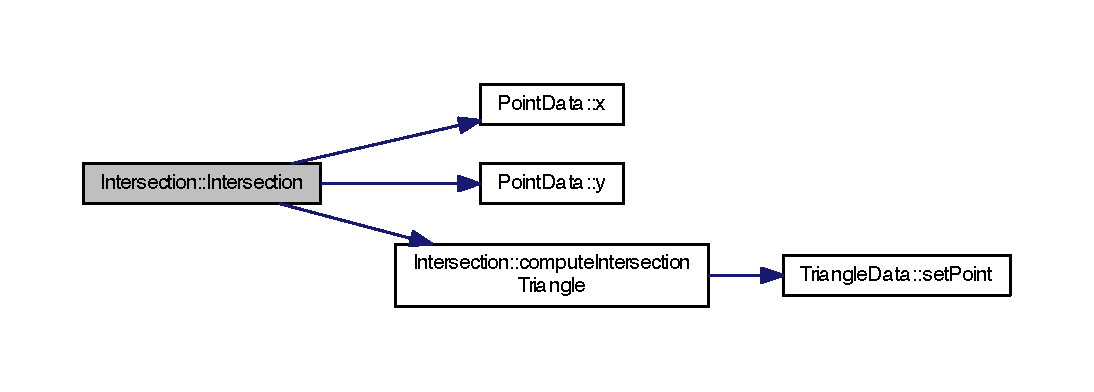
\includegraphics[width=350pt]{classIntersection_ad0bef2cc1bd1f80e72e4b265e19225ca_cgraph}
\end{center}
\end{figure}


\hypertarget{classIntersection_a67497e3efe2793b23909052eeb82c4f3}{\index{Intersection@{Intersection}!Intersection@{Intersection}}
\index{Intersection@{Intersection}!Intersection@{Intersection}}
\subsubsection[{Intersection}]{\setlength{\rightskip}{0pt plus 5cm}Intersection\-::\-Intersection (
\begin{DoxyParamCaption}
{}
\end{DoxyParamCaption}
)\hspace{0.3cm}{\ttfamily [inline]}}}\label{classIntersection_a67497e3efe2793b23909052eeb82c4f3}

\begin{DoxyCode}
77     \{\};
\end{DoxyCode}


\subsection{Documentazione delle funzioni membro}
\hypertarget{classIntersection_ae9d2fb8951a9f5a2bd7c1a96d73226f4}{\index{Intersection@{Intersection}!compute\-Intersection\-Triangle@{compute\-Intersection\-Triangle}}
\index{compute\-Intersection\-Triangle@{compute\-Intersection\-Triangle}!Intersection@{Intersection}}
\subsubsection[{compute\-Intersection\-Triangle}]{\setlength{\rightskip}{0pt plus 5cm}{\bf Triangle\-Data} const \& Intersection\-::compute\-Intersection\-Triangle (
\begin{DoxyParamCaption}
{}
\end{DoxyParamCaption}
)}}\label{classIntersection_ae9d2fb8951a9f5a2bd7c1a96d73226f4}


Funzione che costruisce il triangolo di intersezione. 


\begin{DoxyCode}
144 \{
145     \hyperlink{classPointData}{PointData} point;
146     \textcolor{keyword}{const} scalar\_type tol=1.e-5;
147     scalar\_type s(0.);
148     
149     \textcolor{keywordflow}{for} (size\_type \hyperlink{matrici_8m_a6f6ccfcf58b31cb6412107d9d5281426}{i}=0; \hyperlink{matrici_8m_a6f6ccfcf58b31cb6412107d9d5281426}{i}<3;++\hyperlink{matrici_8m_a6f6ccfcf58b31cb6412107d9d5281426}{i})
150     \{
151         size\_type j = (\hyperlink{matrici_8m_a6f6ccfcf58b31cb6412107d9d5281426}{i} +1 ) % 3;
152         scalar\_type ninj = M\_normals[\hyperlink{matrici_8m_a6f6ccfcf58b31cb6412107d9d5281426}{i}].dot(M\_normals[j] );
153         scalar\_type nitj = M\_normals[\hyperlink{matrici_8m_a6f6ccfcf58b31cb6412107d9d5281426}{i}].dot(M\_tangents[j]);
154         
155         \textcolor{keywordflow}{if}(std::fabs(nitj)<tol)
156         \{
157             point = M\_intersection + 
158                     \hyperlink{classPointData}{PointData} ( M\_normals [ \hyperlink{matrici_8m_a6f6ccfcf58b31cb6412107d9d5281426}{i} ] ( 0 ), M\_normals [ \hyperlink{matrici_8m_a6f6ccfcf58b31cb6412107d9d5281426}{i} ] ( 1 ) ) * ( 0.5 * ( 
      M\_fractures [ j ].getThickness() + M\_fractures [ \hyperlink{matrici_8m_a6f6ccfcf58b31cb6412107d9d5281426}{i} ].getThickness() ));
159         \}
160         \textcolor{keywordflow}{else}
161         \{
162             \textcolor{comment}{// parametric coordinate}
163             s    = 0.5 * ( M\_fractures [ j ].getThickness() * ninj + M\_fractures [ 
      \hyperlink{matrici_8m_a6f6ccfcf58b31cb6412107d9d5281426}{i} ].getThickness() )/nitj;
164         
165             \textcolor{comment}{// the ith point is Pji in the note}
166             point = M\_intersection + ( \hyperlink{classPointData}{PointData} ( M\_tangents [ j ] ( 0 ), M\_tangents [ j ] ( 1 ) 
      ) * s )- 
167                                     ( \hyperlink{classPointData}{PointData} ( M\_normals [ j ] ( 0 ), M\_normals [ j ] ( 1 ) ) *
       ( 0.5 * M\_fractures [ j ].getThickness() ) );
168         \}
169     
170         M\_intersectionTriangle.\hyperlink{classTriangleData_a24c79732610361d5e11ee7ac2d577467}{setPoint}(\hyperlink{matrici_8m_a6f6ccfcf58b31cb6412107d9d5281426}{i},point);
171         
172     \}
173     
174     \textcolor{keywordflow}{return} M\_intersectionTriangle;
175 
176 \}\textcolor{comment}{// computeIntersectionTriangle}
\end{DoxyCode}


Questo è il grafo delle chiamate per questa funzione\-:\nopagebreak
\begin{figure}[H]
\begin{center}
\leavevmode
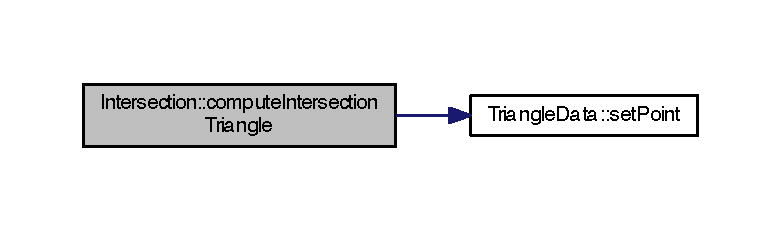
\includegraphics[width=350pt]{classIntersection_ae9d2fb8951a9f5a2bd7c1a96d73226f4_cgraph}
\end{center}
\end{figure}




Questo è il grafo dei chiamanti di questa funzione\-:\nopagebreak
\begin{figure}[H]
\begin{center}
\leavevmode
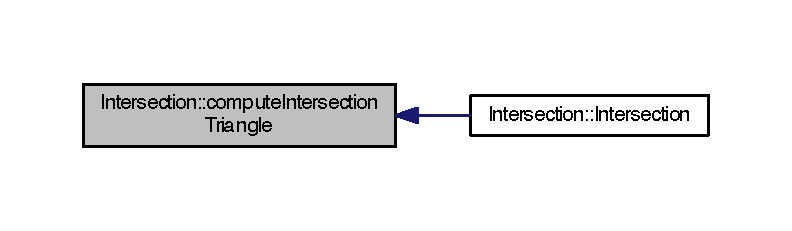
\includegraphics[width=350pt]{classIntersection_ae9d2fb8951a9f5a2bd7c1a96d73226f4_icgraph}
\end{center}
\end{figure}


\hypertarget{classIntersection_abfa3de3a738c4fd36c54eaeecc3557de}{\index{Intersection@{Intersection}!get\-Point\-Intersection@{get\-Point\-Intersection}}
\index{get\-Point\-Intersection@{get\-Point\-Intersection}!Intersection@{Intersection}}
\subsubsection[{get\-Point\-Intersection}]{\setlength{\rightskip}{0pt plus 5cm}{\bf Point\-Data} Intersection\-::get\-Point\-Intersection (
\begin{DoxyParamCaption}
{}
\end{DoxyParamCaption}
) const\hspace{0.3cm}{\ttfamily [inline]}}}\label{classIntersection_abfa3de3a738c4fd36c54eaeecc3557de}


Funzione che restituisce il punto di intersezione. 


\begin{DoxyCode}
113     \{
114         \textcolor{keywordflow}{return} M\_intersection;
115     \}
\end{DoxyCode}


Questo è il grafo dei chiamanti di questa funzione\-:\nopagebreak
\begin{figure}[H]
\begin{center}
\leavevmode
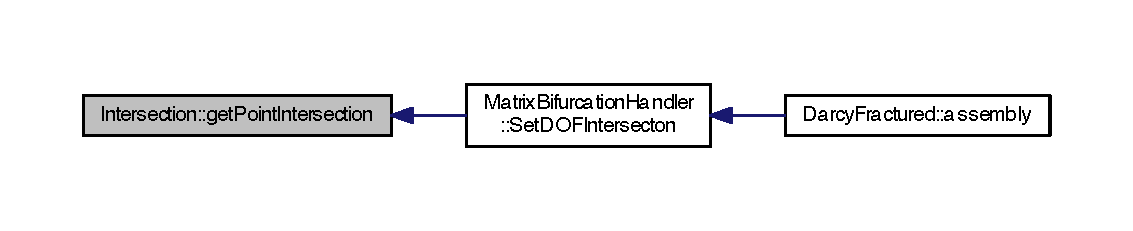
\includegraphics[width=350pt]{classIntersection_abfa3de3a738c4fd36c54eaeecc3557de_icgraph}
\end{center}
\end{figure}


\hypertarget{classIntersection_a603d1cb4b33762c72999968ceec95a39}{\index{Intersection@{Intersection}!intersection\-Triangle@{intersection\-Triangle}}
\index{intersection\-Triangle@{intersection\-Triangle}!Intersection@{Intersection}}
\subsubsection[{intersection\-Triangle}]{\setlength{\rightskip}{0pt plus 5cm}{\bf Triangle\-Data} const\& Intersection\-::intersection\-Triangle (
\begin{DoxyParamCaption}
{}
\end{DoxyParamCaption}
) const\hspace{0.3cm}{\ttfamily [inline]}}}\label{classIntersection_a603d1cb4b33762c72999968ceec95a39}


Funzione che restituisce il triangolo di intersezione. 


\begin{DoxyCode}
105     \{
106         \textcolor{keywordflow}{return} M\_intersectionTriangle;
107     \}
\end{DoxyCode}


Questo è il grafo dei chiamanti di questa funzione\-:\nopagebreak
\begin{figure}[H]
\begin{center}
\leavevmode
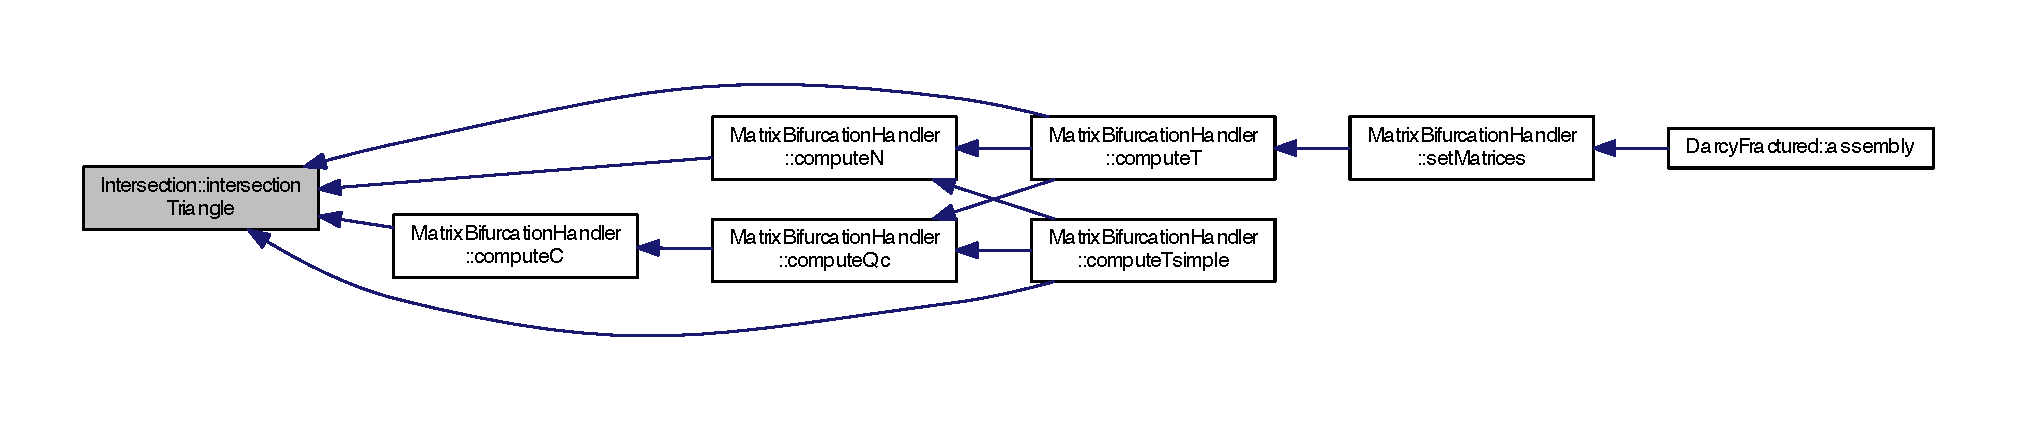
\includegraphics[width=350pt]{classIntersection_a603d1cb4b33762c72999968ceec95a39_icgraph}
\end{center}
\end{figure}


\hypertarget{classIntersection_a9acd54dacf9de3c21fb37df24cb47d06}{\index{Intersection@{Intersection}!is\-Pos@{is\-Pos}}
\index{is\-Pos@{is\-Pos}!Intersection@{Intersection}}
\subsubsection[{is\-Pos}]{\setlength{\rightskip}{0pt plus 5cm}bool Intersection\-::is\-Pos (
\begin{DoxyParamCaption}
\item[{{\bf Fracture\-Handler\-Ptr\-\_\-\-Type} \&}]{fracture, }
\item[{{\bf Fracture\-Handler\-Ptr\-\_\-\-Type} \&}]{otherfracture}
\end{DoxyParamCaption}
)}}\label{classIntersection_a9acd54dacf9de3c21fb37df24cb47d06}


Funzione che mi restituisce vero o falso a seconda se una frattura si trovi o meno nella parte positiva di un'altra. 


\begin{DoxyCode}
237 \{
238     base\_node n0(2);
239     n0 [ 0 ] = 0;
240     n0 [ 1 ] = otherfracture->getLevelSet()->getData()->y\_map ( n0 );
241     n0 [ 0 ] = otherfracture->getLevelSet()->getData()->x\_map ( n0 );
242 
243     base\_node n1(2);
244     n1 [ 0 ] = 1;
245     n1 [ 1 ] = otherfracture->getLevelSet()->getData()->y\_map ( n0 );
246     n1 [ 0 ] = otherfracture->getLevelSet()->getData()->x\_map ( n0 );
247 
248     \textcolor{keywordflow}{if} ( fracture->getLevelSet()->getData()->ylevelSetFunction ( n0 ) >= 0 && fracture->getLevelSet()->
      getData()->ylevelSetFunction ( n1 ) >= 0 )
249         \textcolor{keywordflow}{return} \textcolor{keyword}{true};
250     \textcolor{keywordflow}{else} 
251         \textcolor{keywordflow}{return} \textcolor{keyword}{false};
252     
253 \}\textcolor{comment}{// isPos}
\end{DoxyCode}


Questo è il grafo dei chiamanti di questa funzione\-:\nopagebreak
\begin{figure}[H]
\begin{center}
\leavevmode
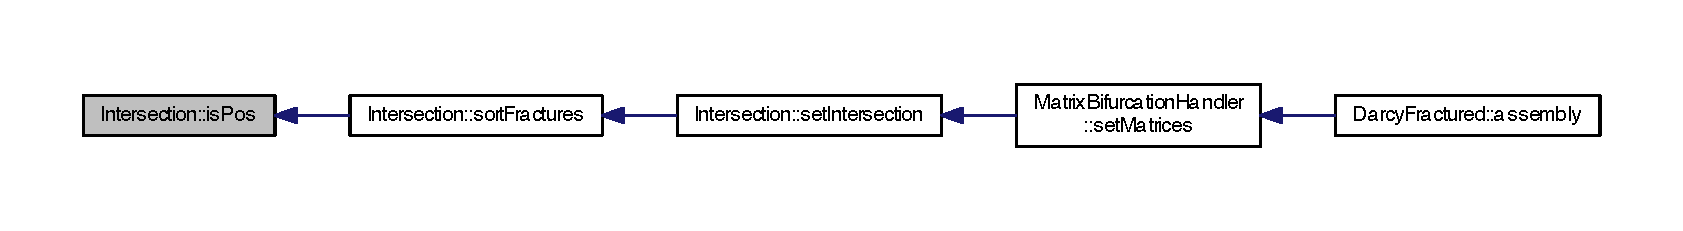
\includegraphics[width=350pt]{classIntersection_a9acd54dacf9de3c21fb37df24cb47d06_icgraph}
\end{center}
\end{figure}


\hypertarget{classIntersection_a8cc823fe1b873994d49bc46b3b4136ef}{\index{Intersection@{Intersection}!operator=@{operator=}}
\index{operator=@{operator=}!Intersection@{Intersection}}
\subsubsection[{operator=}]{\setlength{\rightskip}{0pt plus 5cm}{\bf Intersection}\& Intersection\-::operator= (
\begin{DoxyParamCaption}
\item[{const {\bf Intersection} \&}]{Int}
\end{DoxyParamCaption}
)\hspace{0.3cm}{\ttfamily [inline]}}}\label{classIntersection_a8cc823fe1b873994d49bc46b3b4136ef}

\begin{DoxyCode}
130     \{
131         this-> M\_fractures = Int.M\_fractures;
132         this-> M\_intersection = Int.M\_intersection;
133         
134         this-> M\_tangents [ 0 ] = Int.M\_tangents [ 0 ];
135         this-> M\_tangents [ 1 ] = Int.M\_tangents [ 1 ];
136         this-> M\_tangents [ 2 ] = Int.M\_tangents [ 2 ];
137         
138         this-> M\_normals [ 0 ] = Int.M\_normals [ 0 ];
139         this-> M\_normals [ 1 ] = Int.M\_normals [ 1 ];
140         this-> M\_normals [ 2 ] = Int.M\_normals [ 2 ];
141         
142         this-> M\_intersectionTriangle = Int.M\_intersectionTriangle; 
143         
144         \textcolor{keywordflow}{return} *\textcolor{keyword}{this};
145         
146     \}
\end{DoxyCode}
\hypertarget{classIntersection_ab7a139ac5712a9aa8bb925caf4ecc8af}{\index{Intersection@{Intersection}!set\-Intersection@{set\-Intersection}}
\index{set\-Intersection@{set\-Intersection}!Intersection@{Intersection}}
\subsubsection[{set\-Intersection}]{\setlength{\rightskip}{0pt plus 5cm}void Intersection\-::set\-Intersection (
\begin{DoxyParamCaption}
\item[{{\bf Fracture\-Ptr\-Container\-\_\-\-Type} \&}]{M\-\_\-\-Fractures\-Set}
\end{DoxyParamCaption}
)}}\label{classIntersection_ab7a139ac5712a9aa8bb925caf4ecc8af}


Funzione che costruisce il triangolo di intersezione partendo dal vettore delle fratture che si intersecano. 


\begin{DoxyCode}
49 \{   
50     assert ( M\_FracturesSet.size() == 3 );
51     
52 
53     \textcolor{comment}{// ordino le fratture in senso orario}
54     \hyperlink{classIntersection_ab3bd72c81dc261d3035213e5cefbb1c5}{sortFractures} ( M\_FracturesSet );
55 
56     
57     \textcolor{keyword}{const} size\_type nbDof0 =  M\_FracturesSet [ 0 ]-> getMeshFEMPressure().nb\_basic\_dof();
58     \textcolor{keyword}{const} size\_type nbDof1 =  M\_FracturesSet [ 1 ]-> getMeshFEMPressure().nb\_basic\_dof();
59     \textcolor{keyword}{const} size\_type nbDof2 =  M\_FracturesSet [ 2 ]-> getMeshFEMPressure().nb\_basic\_dof();
60     
61     base\_node node0(2);
62     base\_node node1(2);
63     base\_node node2(2);
64     base\_node nodeI(2);
65     
66     \textcolor{comment}{//truccetto xk y\_map vuole i base\_node}
67     base\_node tmp0( 1 );
68     base\_node tmp1( 1 );
69     tmp0[ 0 ]= 0.;
70     tmp1[ 0 ]= 1.;
71     
72     node0[ 0 ] = M\_FracturesSet [ 0 ]-> getMeshFEMPressure().point\_of\_basic\_dof( 0 )[ 0 ];
73     node1[ 0 ] = M\_FracturesSet [ 1 ]-> getMeshFEMPressure().point\_of\_basic\_dof( 0 )[ 0 ];
74     node2[ 0 ] = M\_FracturesSet [ 2 ]-> getMeshFEMPressure().point\_of\_basic\_dof( 0 )[ 0 ];
75     nodeI[ 0 ] = M\_FracturesSet [ 0 ]-> getMeshFEMPressure().point\_of\_basic\_dof( nbDof0-1 )[ 0 ];
76     
77     node0[ 1 ] = M\_FracturesSet [ 0 ]-> getLevelSet()->getData()->y\_map( tmp0 );
78     node1[ 1 ] = M\_FracturesSet [ 1 ]-> getLevelSet()->getData()->y\_map( tmp0 );
79     node2[ 1 ] = M\_FracturesSet [ 2 ]-> getLevelSet()->getData()->y\_map( tmp0 );
80     nodeI[ 1 ] = M\_FracturesSet [ 0 ]-> getLevelSet()->getData()->y\_map( tmp1 );
81     
82     \textcolor{keywordflow}{if} ( gmm::abs( M\_FracturesSet [ 1 ]-> getLevelSet()->getData()->ylevelSetFunction ( node0 ) ) < 1.0E-2 
      )
83     \{
84         node0 [ 0 ] = M\_FracturesSet [ 0 ]-> getMeshFEMPressure().point\_of\_basic\_dof( nbDof0-1 )[ 0 ];
85         node0 [ 0 ] = M\_FracturesSet [ 0 ]-> getMeshFEMPressure().point\_of\_basic\_dof( nbDof0-1 )[ 0 ];
86         nodeI [ 0 ] = M\_FracturesSet [ 0 ]-> getMeshFEMPressure().point\_of\_basic\_dof( 0 )[ 0 ];
87         node0 [ 1 ] = M\_FracturesSet [ 0 ]-> getLevelSet()->getData()->y\_map( tmp1 );
88         nodeI [ 1 ] = M\_FracturesSet [ 0 ]-> getLevelSet()->getData()->y\_map( tmp0 );
89     \}
90 
91     \textcolor{keywordflow}{if} ( gmm::abs( M\_FracturesSet [ 0 ]-> getLevelSet()->getData()->ylevelSetFunction ( node1 ) ) < 1.0E-2 
      )
92     \{
93         
94         node1 [ 0 ] = M\_FracturesSet [ 1 ]-> getMeshFEMPressure().point\_of\_basic\_dof( nbDof1-1 )[ 0 ];
95         node1 [ 1 ] = M\_FracturesSet [ 1 ]-> getLevelSet()->getData()->y\_map( tmp1 );
96     \}
97 
98     \textcolor{keywordflow}{if} ( gmm::abs( M\_FracturesSet [ 1 ]-> getLevelSet()->getData()->ylevelSetFunction ( node2 ) ) < 1.0E-2 
      )
99     \{
100         node2 [ 0 ] = M\_FracturesSet [ 2 ]-> getMeshFEMPressure().point\_of\_basic\_dof( nbDof2-1 )[ 0 ];
101         node2 [ 1 ] = M\_FracturesSet [ 2 ]-> getLevelSet()->getData()->y\_map( tmp1 );
102     \}
103 
104     \textcolor{comment}{//Estremi liberi delle fratture +  punto di intersezione}
105     \hyperlink{classPointData}{PointData} p0( node0[0], node0[1] );
106     \hyperlink{classPointData}{PointData} p1( node1[0], node1[1] );
107     \hyperlink{classPointData}{PointData} p2( node2[0], node2[1] );
108     \hyperlink{classPointData}{PointData} pi( nodeI[0], nodeI[1] );
109     
110     \textcolor{comment}{//Spessori delle mie fratture}
111     scalar\_type t0,t1,t2;
112     t0 = M\_FracturesSet [ 0 ] -> getData().getThickness();
113     t1 = M\_FracturesSet [ 1 ] -> getData().getThickness();
114     t2 = M\_FracturesSet [ 2 ] -> getData().getThickness();
115     
116 
117     \hyperlink{classFractureEnd}{FractureEnd} f0( p0, t0 );
118     \hyperlink{classFractureEnd}{FractureEnd} f1( p1, t1 );
119     \hyperlink{classFractureEnd}{FractureEnd} f2( p2, t2 );
120     
121     \hyperlink{classIntersection}{Intersection} tmp(f0,f1,f2,pi);
122     
123     this-> M\_fractures = tmp.M\_fractures;
124     this-> M\_intersection = tmp.M\_intersection;
125     
126     this-> M\_tangents [ 0 ] = tmp.M\_tangents [ 0 ];
127     this-> M\_tangents [ 1 ] = tmp.M\_tangents [ 1 ];
128     this-> M\_tangents [ 2 ] = tmp.M\_tangents [ 2 ];
129     
130     this-> M\_normals [ 0 ] = tmp.M\_normals [ 0 ];
131     this-> M\_normals [ 1 ] = tmp.M\_normals [ 1 ];
132     this-> M\_normals [ 2 ] = tmp.M\_normals [ 2 ];
133     
134     this-> M\_intersectionTriangle = tmp.M\_intersectionTriangle; 
135     
136     std::cout << tmp.M\_intersectionTriangle << std::endl;
137     
138     \textcolor{keywordflow}{return};
139     
140 \}\textcolor{comment}{// costruttore intersezione}
\end{DoxyCode}


Questo è il grafo delle chiamate per questa funzione\-:\nopagebreak
\begin{figure}[H]
\begin{center}
\leavevmode
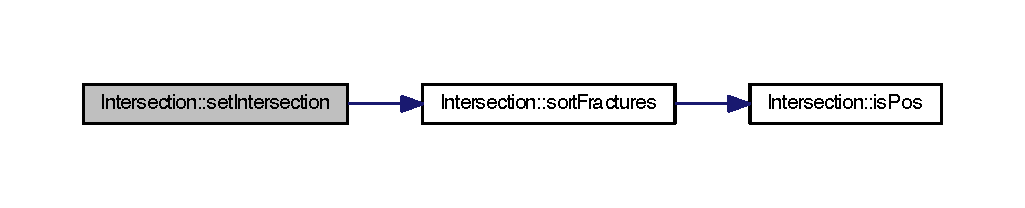
\includegraphics[width=350pt]{classIntersection_ab7a139ac5712a9aa8bb925caf4ecc8af_cgraph}
\end{center}
\end{figure}




Questo è il grafo dei chiamanti di questa funzione\-:\nopagebreak
\begin{figure}[H]
\begin{center}
\leavevmode
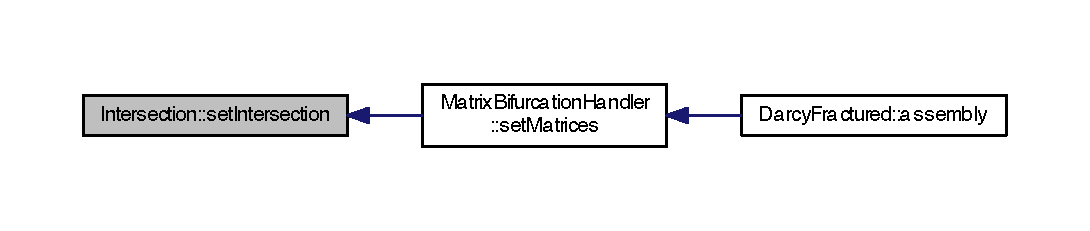
\includegraphics[width=350pt]{classIntersection_ab7a139ac5712a9aa8bb925caf4ecc8af_icgraph}
\end{center}
\end{figure}


\hypertarget{classIntersection_ae071ecb3d3f2d6f9723e310764535883}{\index{Intersection@{Intersection}!set\-Triangle@{set\-Triangle}}
\index{set\-Triangle@{set\-Triangle}!Intersection@{Intersection}}
\subsubsection[{set\-Triangle}]{\setlength{\rightskip}{0pt plus 5cm}void Intersection\-::set\-Triangle (
\begin{DoxyParamCaption}
\item[{const {\bf Triangle\-Data} \&}]{triangle}
\end{DoxyParamCaption}
)\hspace{0.3cm}{\ttfamily [inline]}}}\label{classIntersection_ae071ecb3d3f2d6f9723e310764535883}


Funzione che costruisce il triangolo di intersezione a partire da un triangolo già esistente. 


\begin{DoxyCode}
94     \{
95         M\_intersectionTriangle = triangle;
96         
97         \textcolor{keywordflow}{return};
98     \}
\end{DoxyCode}


Questo è il grafo dei chiamanti di questa funzione\-:\nopagebreak
\begin{figure}[H]
\begin{center}
\leavevmode
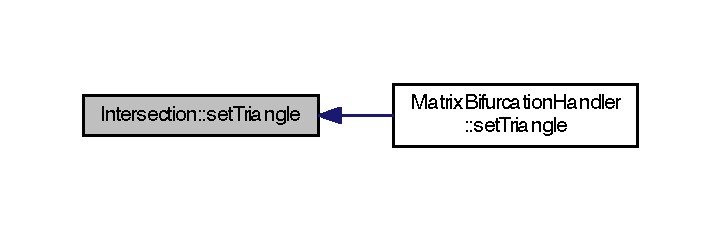
\includegraphics[width=346pt]{classIntersection_ae071ecb3d3f2d6f9723e310764535883_icgraph}
\end{center}
\end{figure}


\hypertarget{classIntersection_ab3bd72c81dc261d3035213e5cefbb1c5}{\index{Intersection@{Intersection}!sort\-Fractures@{sort\-Fractures}}
\index{sort\-Fractures@{sort\-Fractures}!Intersection@{Intersection}}
\subsubsection[{sort\-Fractures}]{\setlength{\rightskip}{0pt plus 5cm}void Intersection\-::sort\-Fractures (
\begin{DoxyParamCaption}
\item[{{\bf Fracture\-Ptr\-Container\-\_\-\-Type} \&}]{M\-\_\-\-Fractures\-Set}
\end{DoxyParamCaption}
)}}\label{classIntersection_ab3bd72c81dc261d3035213e5cefbb1c5}


Funzione che ordina le fratture in senso orario. 


\begin{DoxyCode}
180 \{
181 
182     \hyperlink{FractureHandler_8h_af23fb7a30aaff864bd42587af4f1e78a}{FractureHandlerPtr\_Type} f0 = M\_FracturesSet [ 0 ];
183     \hyperlink{FractureHandler_8h_af23fb7a30aaff864bd42587af4f1e78a}{FractureHandlerPtr\_Type} f1 = M\_FracturesSet [ 1 ];
184     \hyperlink{FractureHandler_8h_af23fb7a30aaff864bd42587af4f1e78a}{FractureHandlerPtr\_Type} f2 = M\_FracturesSet [ 1 ];
185     
186     \textcolor{keywordflow}{if} ( \hyperlink{classIntersection_a9acd54dacf9de3c21fb37df24cb47d06}{isPos} ( f0, f1) )
187     \{   
188         \textcolor{keywordflow}{if} ( !\hyperlink{classIntersection_a9acd54dacf9de3c21fb37df24cb47d06}{isPos} ( f0, f2 ) )
189             \textcolor{keywordflow}{return};
190         \textcolor{keywordflow}{else} \textcolor{keywordflow}{if} ( \hyperlink{classIntersection_a9acd54dacf9de3c21fb37df24cb47d06}{isPos} ( f1, f2 ) )
191             \textcolor{keywordflow}{return};
192         \textcolor{keywordflow}{else}
193         \{   
194             \textcolor{comment}{// devo invertire la due e la uno}
195             \hyperlink{FractureHandler_8h_af23fb7a30aaff864bd42587af4f1e78a}{FractureHandlerPtr\_Type} tmp = f1;
196             M\_FracturesSet [ 1 ] = M\_FracturesSet [ 2 ];
197             M\_FracturesSet [ 2 ] = tmp;
198             
199             \textcolor{keywordflow}{return};
200         \}
201     \}
202         
203     \textcolor{keywordflow}{else} 
204     \{   
205         \textcolor{keywordflow}{if} ( \hyperlink{classIntersection_a9acd54dacf9de3c21fb37df24cb47d06}{isPos} ( f0, f2 ) )
206         \{
207             \textcolor{comment}{// devo invertire la 0 e la 1}
208             \hyperlink{FractureHandler_8h_af23fb7a30aaff864bd42587af4f1e78a}{FractureHandlerPtr\_Type} tmp = f1;
209             M\_FracturesSet [ 1 ] = M\_FracturesSet [ 0 ];
210             M\_FracturesSet [ 0 ] = tmp;
211             
212             \textcolor{keywordflow}{return};
213 
214         \}
215         \textcolor{keywordflow}{else}
216         \{
217             \textcolor{keywordflow}{if} ( \hyperlink{classIntersection_a9acd54dacf9de3c21fb37df24cb47d06}{isPos} ( f1, f2 ) )
218             \{   
219                 \textcolor{comment}{// devo invertire la 2 e la 1}
220                 \hyperlink{FractureHandler_8h_af23fb7a30aaff864bd42587af4f1e78a}{FractureHandlerPtr\_Type} tmp = f1;
221                 M\_FracturesSet [ 1 ] = M\_FracturesSet [ 2 ];
222                 M\_FracturesSet [ 2 ] = tmp;
223                 
224                 \textcolor{keywordflow}{return};
225 
226             \}
227 
228         \}
229     \}
230     
231     \textcolor{keywordflow}{return};
232 \}\textcolor{comment}{// sortFractures}
\end{DoxyCode}


Questo è il grafo delle chiamate per questa funzione\-:\nopagebreak
\begin{figure}[H]
\begin{center}
\leavevmode
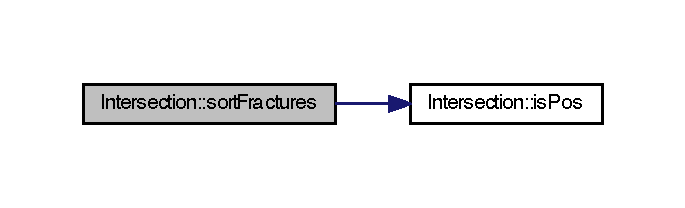
\includegraphics[width=329pt]{classIntersection_ab3bd72c81dc261d3035213e5cefbb1c5_cgraph}
\end{center}
\end{figure}




Questo è il grafo dei chiamanti di questa funzione\-:\nopagebreak
\begin{figure}[H]
\begin{center}
\leavevmode
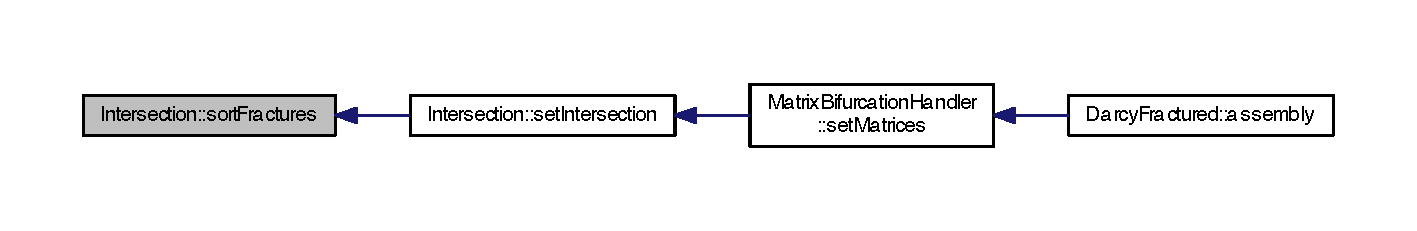
\includegraphics[width=350pt]{classIntersection_ab3bd72c81dc261d3035213e5cefbb1c5_icgraph}
\end{center}
\end{figure}




La documentazione per questa classe è stata generata a partire dai seguenti file\-:\begin{DoxyCompactItemize}
\item 
include/\hyperlink{TriangleHandler_8h}{Triangle\-Handler.\-h}\item 
src/\hyperlink{TriangleHandler_8cc}{Triangle\-Handler.\-cc}\end{DoxyCompactItemize}

\hypertarget{classgetfem_1_1level__set__unit__normal}{\section{Riferimenti per la classe getfem\-:\-:level\-\_\-set\-\_\-unit\-\_\-normal}
\label{classgetfem_1_1level__set__unit__normal}\index{getfem\-::level\-\_\-set\-\_\-unit\-\_\-normal@{getfem\-::level\-\_\-set\-\_\-unit\-\_\-normal}}
}


Classe che rappresenta la normale ad un levelset.  




{\ttfamily \#include $<$X\-F\-E\-M\-Operators.\-h$>$}



Diagramma delle classi per getfem\-:\-:level\-\_\-set\-\_\-unit\-\_\-normal\nopagebreak
\begin{figure}[H]
\begin{center}
\leavevmode
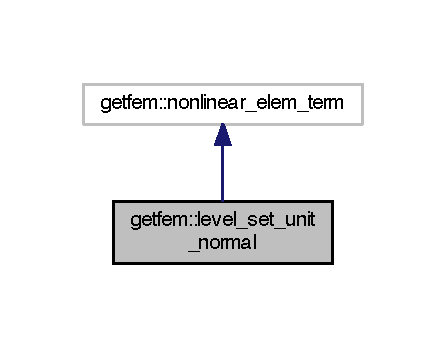
\includegraphics[width=214pt]{classgetfem_1_1level__set__unit__normal__inherit__graph}
\end{center}
\end{figure}


Diagramma di collaborazione per getfem\-:\-:level\-\_\-set\-\_\-unit\-\_\-normal\-:\nopagebreak
\begin{figure}[H]
\begin{center}
\leavevmode
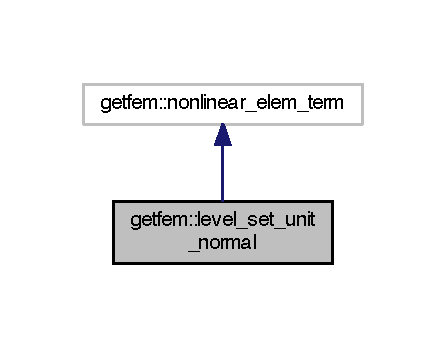
\includegraphics[width=214pt]{classgetfem_1_1level__set__unit__normal__coll__graph}
\end{center}
\end{figure}
\subsection*{Membri pubblici}
\begin{DoxyCompactItemize}
\item 
\hyperlink{classgetfem_1_1level__set__unit__normal_ab3614c6046c7f4875bf7f295dc858463}{level\-\_\-set\-\_\-unit\-\_\-normal} (const getfem\-::mesh\-\_\-fem \&mf\-\_\-, const \hyperlink{Core_8h_a4e75b5863535ba1dd79942de2846eff0}{scalar\-Vector\-\_\-\-Type} \&U\-\_\-)
\item 
const bgeot\-::multi\-\_\-index \& \hyperlink{classgetfem_1_1level__set__unit__normal_a752cfcceeb76e736146a75ee676366a1}{sizes} () const 
\item 
virtual void \hyperlink{classgetfem_1_1level__set__unit__normal_ad1c18b6cbd9bad011fc00198d06b62f8}{compute} (getfem\-::fem\-\_\-interpolation\-\_\-context \&ctx, bgeot\-::base\-\_\-tensor \&t)
\end{DoxyCompactItemize}


\subsection{Descrizione dettagliata}
Classe che rappresenta la normale ad un levelset. 

\subsection{Documentazione dei costruttori e dei distruttori}
\hypertarget{classgetfem_1_1level__set__unit__normal_ab3614c6046c7f4875bf7f295dc858463}{\index{getfem\-::level\-\_\-set\-\_\-unit\-\_\-normal@{getfem\-::level\-\_\-set\-\_\-unit\-\_\-normal}!level\-\_\-set\-\_\-unit\-\_\-normal@{level\-\_\-set\-\_\-unit\-\_\-normal}}
\index{level\-\_\-set\-\_\-unit\-\_\-normal@{level\-\_\-set\-\_\-unit\-\_\-normal}!getfem::level_set_unit_normal@{getfem\-::level\-\_\-set\-\_\-unit\-\_\-normal}}
\subsubsection[{level\-\_\-set\-\_\-unit\-\_\-normal}]{\setlength{\rightskip}{0pt plus 5cm}getfem\-::level\-\_\-set\-\_\-unit\-\_\-normal\-::level\-\_\-set\-\_\-unit\-\_\-normal (
\begin{DoxyParamCaption}
\item[{const getfem\-::mesh\-\_\-fem \&}]{mf\-\_\-, }
\item[{const {\bf scalar\-Vector\-\_\-\-Type} \&}]{U\-\_\-}
\end{DoxyParamCaption}
)}}\label{classgetfem_1_1level__set__unit__normal_ab3614c6046c7f4875bf7f295dc858463}

\begin{DoxyCode}
12                                                                                                       :
13     mf(mf\_), U(mf\_.nb\_basic\_dof()), N(mf\_.linked\_mesh().dim()), gradU(1, N)
14 \{
15     sizes\_.resize(1);
16     sizes\_ [ 0 ] = short\_type(N);
17     mf.extend\_vector(U\_, U);
18 \}
\end{DoxyCode}


\subsection{Documentazione delle funzioni membro}
\hypertarget{classgetfem_1_1level__set__unit__normal_ad1c18b6cbd9bad011fc00198d06b62f8}{\index{getfem\-::level\-\_\-set\-\_\-unit\-\_\-normal@{getfem\-::level\-\_\-set\-\_\-unit\-\_\-normal}!compute@{compute}}
\index{compute@{compute}!getfem::level_set_unit_normal@{getfem\-::level\-\_\-set\-\_\-unit\-\_\-normal}}
\subsubsection[{compute}]{\setlength{\rightskip}{0pt plus 5cm}void getfem\-::level\-\_\-set\-\_\-unit\-\_\-normal\-::compute (
\begin{DoxyParamCaption}
\item[{getfem\-::fem\-\_\-interpolation\-\_\-context \&}]{ctx, }
\item[{bgeot\-::base\-\_\-tensor \&}]{t}
\end{DoxyParamCaption}
)\hspace{0.3cm}{\ttfamily [virtual]}}}\label{classgetfem_1_1level__set__unit__normal_ad1c18b6cbd9bad011fc00198d06b62f8}

\begin{DoxyCode}
21 \{
22     size\_type cv = ctx.convex\_num();
23     coeff.resize(mf.nb\_basic\_dof\_of\_element(cv));
24     
25     gmm::copy( gmm::sub\_vector( U, gmm::sub\_index( mf.ind\_basic\_dof\_of\_element( cv ) ) ), coeff );
26 
27     ctx.pf()->interpolation\_grad( ctx, coeff, gradU, 1);
28     
29     scalar\_type norm = gmm::vect\_norm2( gmm::mat\_row( gradU, 0 ));
30     
31     \textcolor{keywordflow}{for} ( size\_type \hyperlink{matrici_8m_a6f6ccfcf58b31cb6412107d9d5281426}{i} = 0; \hyperlink{matrici_8m_a6f6ccfcf58b31cb6412107d9d5281426}{i} < N; ++\hyperlink{matrici_8m_a6f6ccfcf58b31cb6412107d9d5281426}{i} )
32     \{
33         t [ \hyperlink{matrici_8m_a6f6ccfcf58b31cb6412107d9d5281426}{i} ] = gradU(0, \hyperlink{matrici_8m_a6f6ccfcf58b31cb6412107d9d5281426}{i}) / norm;
34     \}
35     
36     \textcolor{keywordflow}{return};
37 \}
\end{DoxyCode}
\hypertarget{classgetfem_1_1level__set__unit__normal_a752cfcceeb76e736146a75ee676366a1}{\index{getfem\-::level\-\_\-set\-\_\-unit\-\_\-normal@{getfem\-::level\-\_\-set\-\_\-unit\-\_\-normal}!sizes@{sizes}}
\index{sizes@{sizes}!getfem::level_set_unit_normal@{getfem\-::level\-\_\-set\-\_\-unit\-\_\-normal}}
\subsubsection[{sizes}]{\setlength{\rightskip}{0pt plus 5cm}const bgeot\-::multi\-\_\-index\& getfem\-::level\-\_\-set\-\_\-unit\-\_\-normal\-::sizes (
\begin{DoxyParamCaption}
{}
\end{DoxyParamCaption}
) const\hspace{0.3cm}{\ttfamily [inline]}}}\label{classgetfem_1_1level__set__unit__normal_a752cfcceeb76e736146a75ee676366a1}

\begin{DoxyCode}
32     \{
33         \textcolor{keywordflow}{return} sizes\_;
34     \}
\end{DoxyCode}


La documentazione per questa classe è stata generata a partire dai seguenti file\-:\begin{DoxyCompactItemize}
\item 
include/\hyperlink{XFEMOperators_8h}{X\-F\-E\-M\-Operators.\-h}\item 
src/\hyperlink{XFEMOperators_8cc}{X\-F\-E\-M\-Operators.\-cc}\end{DoxyCompactItemize}

\hypertarget{classLevelSetData}{\section{Riferimenti per la classe Level\-Set\-Data}
\label{classLevelSetData}\index{Level\-Set\-Data@{Level\-Set\-Data}}
}


\hyperlink{LevelSetData_8h}{Level\-Set\-Data.\-h}.  




{\ttfamily \#include $<$Level\-Set\-Data.\-h$>$}

\subsection*{Membri pubblici}
\begin{DoxyCompactItemize}
\item 
\hyperlink{classLevelSetData_a8b2ab7808f47d9a951327891d65e84be}{Level\-Set\-Data} (const Get\-Pot \&data\-File, const std\-::string \&section=\char`\"{}fracture\-Data/\char`\"{}, const std\-::string \&section\-Level\-Set=\char`\"{}level\-Set/\char`\"{})
\item 
scalar\-\_\-type \hyperlink{classLevelSetData_a732ae59581206d4f94237e54bc0071e3}{ylevel\-Set\-Function} (const base\-\_\-node \&x)
\begin{DoxyCompactList}\small\item\em Questa funzione definisce il level set che rappresenta la frattura, level set valutato in (x,y). \end{DoxyCompactList}\item 
scalar\-\_\-type \hyperlink{classLevelSetData_a665241939c12bad26face4d997e655ce}{level\-Set\-Function} (const base\-\_\-node \&x)
\begin{DoxyCompactList}\small\item\em Questa funzione definisce il level set che rappresenta la frattura, level set valutato in (t,y). \end{DoxyCompactList}\item 
scalar\-\_\-type \hyperlink{classLevelSetData_a60ea6aa9991dfdae4e4a3950ed8db66c}{level\-Set\-Cut\-Function} (const base\-\_\-node \&x)
\begin{DoxyCompactList}\small\item\em scalar\-\_\-type level\-Set\-Cut\-Function ( const base\-\_\-node\& x, int num = 0 ) \end{DoxyCompactList}\item 
scalar\-\_\-type \hyperlink{classLevelSetData_aa4cda1cced4bc385d85383b40bbc2631}{y\-\_\-map} (const base\-\_\-node \&t)
\begin{DoxyCompactList}\small\item\em Questa funzione rappresenta la mappa dalla frattura piatta, y(t). \end{DoxyCompactList}\item 
scalar\-\_\-type \hyperlink{classLevelSetData_ae7f10d3f10b72fbb6f703ba7aa8fe17b}{x\-\_\-map} (const base\-\_\-node \&t)
\begin{DoxyCompactList}\small\item\em Questa funzione rappresenta la mappa dalla frattura piatta, x(t). \end{DoxyCompactList}\item 
\hyperlink{Core_8h_a4e75b5863535ba1dd79942de2846eff0}{scalar\-Vector\-\_\-\-Type} \hyperlink{classLevelSetData_a40fcfa36de7ac76613284d03690eb54b}{map\-\_\-jac} (const base\-\_\-node \&x, const size\-\_\-type \&num)
\begin{DoxyCompactList}\small\item\em Questa funzione serve per convertire la lunghezza/area degli elementi dalla frattura piatta a quella mappata. \end{DoxyCompactList}\item 
\hyperlink{Core_8h_a4e75b5863535ba1dd79942de2846eff0}{scalar\-Vector\-\_\-\-Type} \hyperlink{classLevelSetData_a674d56690f4e22cbca38bf4b5f176a5e}{normal\-\_\-map} (const base\-\_\-node \&P, const size\-\_\-type \&num)
\begin{DoxyCompactList}\small\item\em Funzione che calcola la normale alla frattura -\/ può anche dipendere da x. \end{DoxyCompactList}\item 
bgeot\-::dim\-\_\-type \hyperlink{classLevelSetData_aa4c3e1f7876cd318e80f5052689fe9e3}{get\-Space\-Dimension} () const 
\item 
std\-::string \hyperlink{classLevelSetData_a3f8cb21a929065136dcf3a449edb373a}{get\-Integration\-Type\-Simplex} () const 
\item 
std\-::string \hyperlink{classLevelSetData_a672418971ce9b1bf71d3c6bccd278bd7}{get\-Level\-Set\-Function\-String} () const 
\end{DoxyCompactItemize}


\subsection{Descrizione dettagliata}
\hyperlink{LevelSetData_8h}{Level\-Set\-Data.\-h}. 

Classe che contiene tutte le informazioni legate al level set e le funzioni per valutarne il valore nei punti 

\subsection{Documentazione dei costruttori e dei distruttori}
\hypertarget{classLevelSetData_a8b2ab7808f47d9a951327891d65e84be}{\index{Level\-Set\-Data@{Level\-Set\-Data}!Level\-Set\-Data@{Level\-Set\-Data}}
\index{Level\-Set\-Data@{Level\-Set\-Data}!LevelSetData@{Level\-Set\-Data}}
\subsubsection[{Level\-Set\-Data}]{\setlength{\rightskip}{0pt plus 5cm}Level\-Set\-Data\-::\-Level\-Set\-Data (
\begin{DoxyParamCaption}
\item[{const Get\-Pot \&}]{data\-File, }
\item[{const std\-::string \&}]{section = {\ttfamily \char`\"{}fractureData/\char`\"{}}, }
\item[{const std\-::string \&}]{section\-Level\-Set = {\ttfamily \char`\"{}levelSet/\char`\"{}}}
\end{DoxyParamCaption}
)}}\label{classLevelSetData_a8b2ab7808f47d9a951327891d65e84be}

\begin{DoxyCode}
11                                                                 :
12             M\_section ( section ),
13             M\_sectionLevelSet ( M\_section + sectionLevelSet ),
14             M\_spaceDimension ( dataFile ( ( M\_section + \textcolor{stringliteral}{"spaceDimension"} ).data (), 1. ) ),
15             \textcolor{comment}{// level set}
16             M\_function ( dataFile ( ( M\_sectionLevelSet + \textcolor{stringliteral}{"levelSet"} ).data (), \textcolor{stringliteral}{"x"} ) ),
17             M\_xfunction ( dataFile ( ( M\_sectionLevelSet + \textcolor{stringliteral}{"xlevelSet"} ).data (), \textcolor{stringliteral}{"t"} ) ),
18             M\_yfunction ( dataFile ( ( M\_sectionLevelSet + \textcolor{stringliteral}{"ylevelSet"} ).data (), \textcolor{stringliteral}{"t"} ) ),
19             M\_cutFunction ( dataFile ( ( M\_sectionLevelSet + \textcolor{stringliteral}{"levelSetCut"} ).data (), \textcolor{stringliteral}{"-1"} ) ),
20             M\_x\_map ( dataFile ( ( M\_sectionLevelSet + \textcolor{stringliteral}{"xMap"} ).data (), \textcolor{stringliteral}{"1"} ) ),
21             M\_y\_map ( dataFile ( ( M\_sectionLevelSet + \textcolor{stringliteral}{"yMap"} ).data (), \textcolor{stringliteral}{"1"} ) ),
22             M\_map\_jac ( dataFile ( ( M\_sectionLevelSet + \textcolor{stringliteral}{"jacMap"} ).data (), \textcolor{stringliteral}{"1"} ) ),
23             M\_normal\_map ( dataFile ( ( M\_sectionLevelSet + \textcolor{stringliteral}{"normalMap"} ).data (), \textcolor{stringliteral}{"1"} ) ),
24             M\_integrationTypeSimplex ( dataFile ( ( M\_sectionLevelSet + \textcolor{stringliteral}{"integrationTypeSimplex"} ).data (),
25                                                   \textcolor{stringliteral}{"IM\_STRUCTURED\_COMPOSITE(IM\_TRIANGLE(3),1)"} ) )
26 \{\}
\end{DoxyCode}


\subsection{Documentazione delle funzioni membro}
\hypertarget{classLevelSetData_a3f8cb21a929065136dcf3a449edb373a}{\index{Level\-Set\-Data@{Level\-Set\-Data}!get\-Integration\-Type\-Simplex@{get\-Integration\-Type\-Simplex}}
\index{get\-Integration\-Type\-Simplex@{get\-Integration\-Type\-Simplex}!LevelSetData@{Level\-Set\-Data}}
\subsubsection[{get\-Integration\-Type\-Simplex}]{\setlength{\rightskip}{0pt plus 5cm}std\-::string Level\-Set\-Data\-::get\-Integration\-Type\-Simplex (
\begin{DoxyParamCaption}
{}
\end{DoxyParamCaption}
) const\hspace{0.3cm}{\ttfamily [inline]}}}\label{classLevelSetData_a3f8cb21a929065136dcf3a449edb373a}

\begin{DoxyCode}
81     \{
82         \textcolor{keywordflow}{return} M\_integrationTypeSimplex;
83     \}
\end{DoxyCode}
\hypertarget{classLevelSetData_a672418971ce9b1bf71d3c6bccd278bd7}{\index{Level\-Set\-Data@{Level\-Set\-Data}!get\-Level\-Set\-Function\-String@{get\-Level\-Set\-Function\-String}}
\index{get\-Level\-Set\-Function\-String@{get\-Level\-Set\-Function\-String}!LevelSetData@{Level\-Set\-Data}}
\subsubsection[{get\-Level\-Set\-Function\-String}]{\setlength{\rightskip}{0pt plus 5cm}std\-::string Level\-Set\-Data\-::get\-Level\-Set\-Function\-String (
\begin{DoxyParamCaption}
{}
\end{DoxyParamCaption}
) const\hspace{0.3cm}{\ttfamily [inline]}}}\label{classLevelSetData_a672418971ce9b1bf71d3c6bccd278bd7}

\begin{DoxyCode}
87     \{
88         \textcolor{keywordflow}{return} M\_yfunction;
89     \}
\end{DoxyCode}
\hypertarget{classLevelSetData_aa4c3e1f7876cd318e80f5052689fe9e3}{\index{Level\-Set\-Data@{Level\-Set\-Data}!get\-Space\-Dimension@{get\-Space\-Dimension}}
\index{get\-Space\-Dimension@{get\-Space\-Dimension}!LevelSetData@{Level\-Set\-Data}}
\subsubsection[{get\-Space\-Dimension}]{\setlength{\rightskip}{0pt plus 5cm}bgeot\-::dim\-\_\-type Level\-Set\-Data\-::get\-Space\-Dimension (
\begin{DoxyParamCaption}
{}
\end{DoxyParamCaption}
) const\hspace{0.3cm}{\ttfamily [inline]}}}\label{classLevelSetData_aa4c3e1f7876cd318e80f5052689fe9e3}

\begin{DoxyCode}
75     \{
76         \textcolor{keywordflow}{return} M\_spaceDimension;
77     \}
\end{DoxyCode}
\hypertarget{classLevelSetData_a60ea6aa9991dfdae4e4a3950ed8db66c}{\index{Level\-Set\-Data@{Level\-Set\-Data}!level\-Set\-Cut\-Function@{level\-Set\-Cut\-Function}}
\index{level\-Set\-Cut\-Function@{level\-Set\-Cut\-Function}!LevelSetData@{Level\-Set\-Data}}
\subsubsection[{level\-Set\-Cut\-Function}]{\setlength{\rightskip}{0pt plus 5cm}scalar\-\_\-type Level\-Set\-Data\-::level\-Set\-Cut\-Function (
\begin{DoxyParamCaption}
\item[{const base\-\_\-node \&}]{x}
\end{DoxyParamCaption}
)}}\label{classLevelSetData_a60ea6aa9991dfdae4e4a3950ed8db66c}


scalar\-\_\-type level\-Set\-Cut\-Function ( const base\-\_\-node\& x, int num = 0 ) 

Questa funzione definisce il level set che rappresenta la frattura, se per caso voglio \char`\"{}tagliare la frattura\char`\"{}. 
\begin{DoxyParams}{Parametri}
{\em base\-\_\-node\&} & x\-: nodo in coordinate ( t, y ) in cui valutare il levelset \\
\hline
\end{DoxyParams}
\begin{DoxyReturn}{Restituisce}
scalar\-\_\-type\-: valore del levelset nel nodo x 
\end{DoxyReturn}

\begin{DoxyCode}
50 \{
51     M\_parser.\hyperlink{classLifeV_1_1Parser_ac05769e836a0dc95d9c020df361a5194}{setString} ( M\_cutFunction );
52     M\_parser.\hyperlink{classLifeV_1_1Parser_aa2b362e12b8feb60231705d499c9fbae}{setVariable} ( \textcolor{stringliteral}{"t"}, t [ 0 ] );
53     M\_parser.\hyperlink{classLifeV_1_1Parser_aa2b362e12b8feb60231705d499c9fbae}{setVariable} ( \textcolor{stringliteral}{"y"}, t [ 1 ] );
54     
55     \textcolor{keywordflow}{return} M\_parser.\hyperlink{classLifeV_1_1Parser_a51d84fd4ae6d420620e7beee58fad673}{evaluate} ();
56 \}
\end{DoxyCode}


Questo è il grafo delle chiamate per questa funzione\-:\nopagebreak
\begin{figure}[H]
\begin{center}
\leavevmode
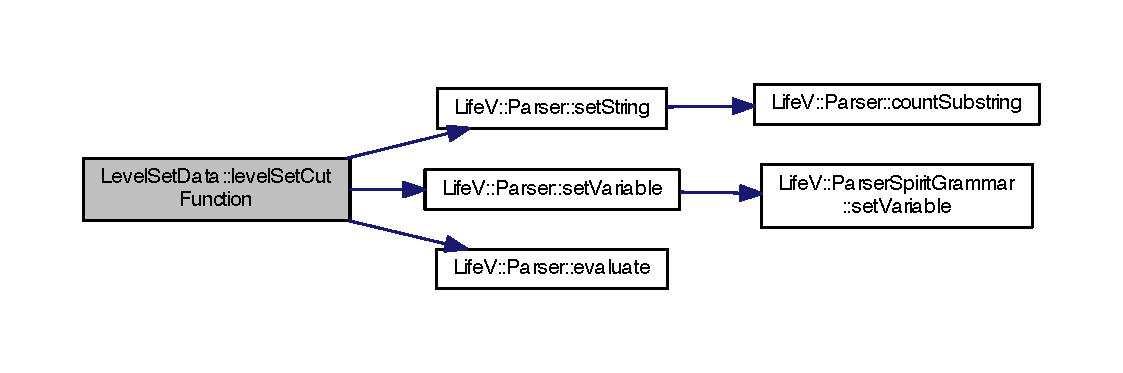
\includegraphics[width=350pt]{classLevelSetData_a60ea6aa9991dfdae4e4a3950ed8db66c_cgraph}
\end{center}
\end{figure}


\hypertarget{classLevelSetData_a665241939c12bad26face4d997e655ce}{\index{Level\-Set\-Data@{Level\-Set\-Data}!level\-Set\-Function@{level\-Set\-Function}}
\index{level\-Set\-Function@{level\-Set\-Function}!LevelSetData@{Level\-Set\-Data}}
\subsubsection[{level\-Set\-Function}]{\setlength{\rightskip}{0pt plus 5cm}scalar\-\_\-type Level\-Set\-Data\-::level\-Set\-Function (
\begin{DoxyParamCaption}
\item[{const base\-\_\-node \&}]{x}
\end{DoxyParamCaption}
)}}\label{classLevelSetData_a665241939c12bad26face4d997e655ce}


Questa funzione definisce il level set che rappresenta la frattura, level set valutato in (t,y). 


\begin{DoxyParams}{Parametri}
{\em base\-\_\-node\&} & x\-: nodo in coordinate ( t, y ) in cui valutare il levelset \\
\hline
\end{DoxyParams}
\begin{DoxyReturn}{Restituisce}
scalar\-\_\-type\-: valore del levelset nel nodo x 
\end{DoxyReturn}

\begin{DoxyCode}
40 \{
41     M\_parser.\hyperlink{classLifeV_1_1Parser_ac05769e836a0dc95d9c020df361a5194}{setString} ( M\_yfunction );
42     M\_parser.\hyperlink{classLifeV_1_1Parser_aa2b362e12b8feb60231705d499c9fbae}{setVariable} ( \textcolor{stringliteral}{"t"}, t [ 0 ] );
43     M\_parser.\hyperlink{classLifeV_1_1Parser_aa2b362e12b8feb60231705d499c9fbae}{setVariable} ( \textcolor{stringliteral}{"y"}, t [ 1 ] );
44     
45     \textcolor{keywordflow}{return} M\_parser.\hyperlink{classLifeV_1_1Parser_a51d84fd4ae6d420620e7beee58fad673}{evaluate} ();
46 \}
\end{DoxyCode}


Questo è il grafo delle chiamate per questa funzione\-:\nopagebreak
\begin{figure}[H]
\begin{center}
\leavevmode
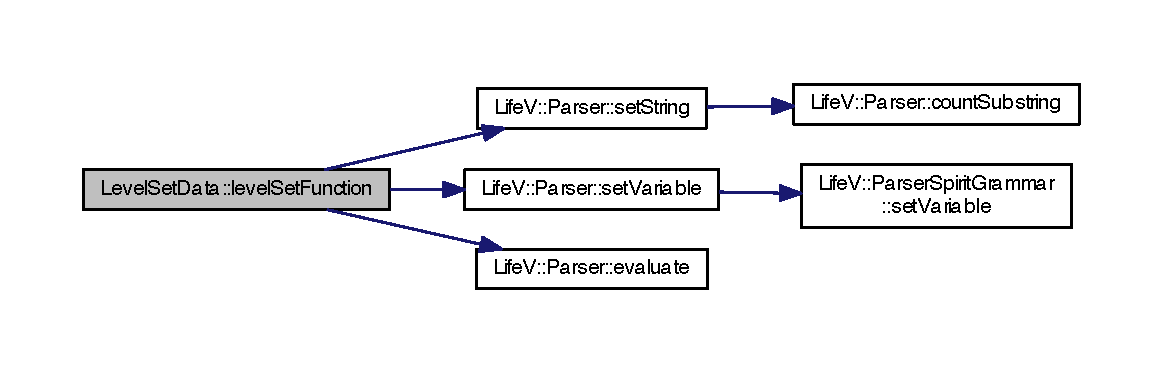
\includegraphics[width=350pt]{classLevelSetData_a665241939c12bad26face4d997e655ce_cgraph}
\end{center}
\end{figure}


\hypertarget{classLevelSetData_a40fcfa36de7ac76613284d03690eb54b}{\index{Level\-Set\-Data@{Level\-Set\-Data}!map\-\_\-jac@{map\-\_\-jac}}
\index{map\-\_\-jac@{map\-\_\-jac}!LevelSetData@{Level\-Set\-Data}}
\subsubsection[{map\-\_\-jac}]{\setlength{\rightskip}{0pt plus 5cm}{\bf scalar\-Vector\-\_\-\-Type} Level\-Set\-Data\-::map\-\_\-jac (
\begin{DoxyParamCaption}
\item[{const base\-\_\-node \&}]{x, }
\item[{const size\-\_\-type \&}]{num}
\end{DoxyParamCaption}
)}}\label{classLevelSetData_a40fcfa36de7ac76613284d03690eb54b}


Questa funzione serve per convertire la lunghezza/area degli elementi dalla frattura piatta a quella mappata. 


\begin{DoxyCode}
79 \{
80     \hyperlink{Core_8h_a4e75b5863535ba1dd79942de2846eff0}{scalarVector\_Type} \hyperlink{classLevelSetData_a40fcfa36de7ac76613284d03690eb54b}{map\_jac} ( num, 0. );
81 
82     M\_parser.\hyperlink{classLifeV_1_1Parser_ac05769e836a0dc95d9c020df361a5194}{setString} ( M\_map\_jac );
83     M\_parser.\hyperlink{classLifeV_1_1Parser_aa2b362e12b8feb60231705d499c9fbae}{setVariable} ( \textcolor{stringliteral}{"x"}, x [ 0 ] );
84     M\_parser.\hyperlink{classLifeV_1_1Parser_aa2b362e12b8feb60231705d499c9fbae}{setVariable} ( \textcolor{stringliteral}{"y"}, x [ 1 ] );
85 
86     \textcolor{keywordflow}{for} ( size\_type \hyperlink{matrici_8m_a6f6ccfcf58b31cb6412107d9d5281426}{i} = 0; \hyperlink{matrici_8m_a6f6ccfcf58b31cb6412107d9d5281426}{i} < num; ++\hyperlink{matrici_8m_a6f6ccfcf58b31cb6412107d9d5281426}{i} )
87     \{
88         \hyperlink{classLevelSetData_a40fcfa36de7ac76613284d03690eb54b}{map\_jac} [ \hyperlink{matrici_8m_a6f6ccfcf58b31cb6412107d9d5281426}{i} ] = M\_parser.\hyperlink{classLifeV_1_1Parser_a51d84fd4ae6d420620e7beee58fad673}{evaluate} ( \hyperlink{matrici_8m_a6f6ccfcf58b31cb6412107d9d5281426}{i} );
89     \}
90 
91     \textcolor{keywordflow}{return} \hyperlink{classLevelSetData_a40fcfa36de7ac76613284d03690eb54b}{map\_jac};
92 \}
\end{DoxyCode}


Questo è il grafo delle chiamate per questa funzione\-:\nopagebreak
\begin{figure}[H]
\begin{center}
\leavevmode
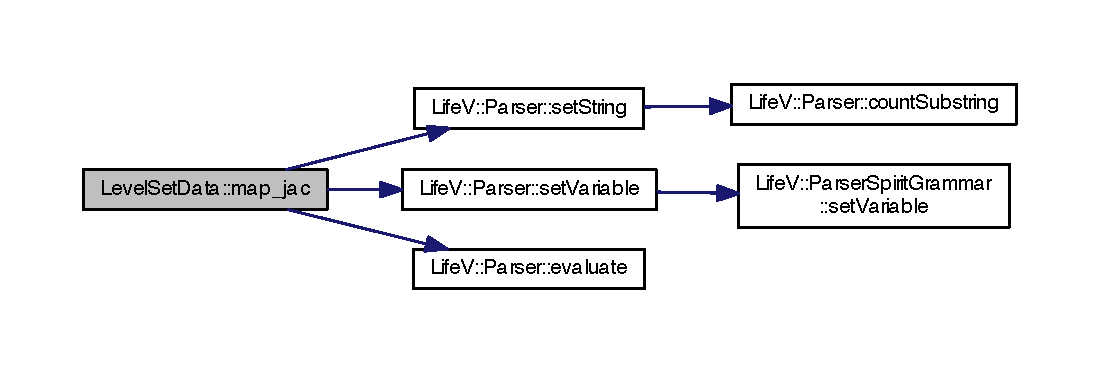
\includegraphics[width=350pt]{classLevelSetData_a40fcfa36de7ac76613284d03690eb54b_cgraph}
\end{center}
\end{figure}


\hypertarget{classLevelSetData_a674d56690f4e22cbca38bf4b5f176a5e}{\index{Level\-Set\-Data@{Level\-Set\-Data}!normal\-\_\-map@{normal\-\_\-map}}
\index{normal\-\_\-map@{normal\-\_\-map}!LevelSetData@{Level\-Set\-Data}}
\subsubsection[{normal\-\_\-map}]{\setlength{\rightskip}{0pt plus 5cm}{\bf scalar\-Vector\-\_\-\-Type} Level\-Set\-Data\-::normal\-\_\-map (
\begin{DoxyParamCaption}
\item[{const base\-\_\-node \&}]{P, }
\item[{const size\-\_\-type \&}]{num}
\end{DoxyParamCaption}
)}}\label{classLevelSetData_a674d56690f4e22cbca38bf4b5f176a5e}


Funzione che calcola la normale alla frattura -\/ può anche dipendere da x. 


\begin{DoxyCode}
97 \{
98     \hyperlink{Core_8h_a4e75b5863535ba1dd79942de2846eff0}{scalarVector\_Type} \hyperlink{classLevelSetData_a674d56690f4e22cbca38bf4b5f176a5e}{normal\_map} ( num + 1, 0. );
99 
100     M\_parser.\hyperlink{classLifeV_1_1Parser_ac05769e836a0dc95d9c020df361a5194}{setString} ( M\_map\_jac );
101     M\_parser.\hyperlink{classLifeV_1_1Parser_aa2b362e12b8feb60231705d499c9fbae}{setVariable} ( \textcolor{stringliteral}{"x"}, x [ 0 ] );
102     M\_parser.\hyperlink{classLifeV_1_1Parser_aa2b362e12b8feb60231705d499c9fbae}{setVariable} ( \textcolor{stringliteral}{"y"}, x [ 1 ] );
103 
104     \textcolor{keywordflow}{for} ( size\_type \hyperlink{matrici_8m_a6f6ccfcf58b31cb6412107d9d5281426}{i} = 0; \hyperlink{matrici_8m_a6f6ccfcf58b31cb6412107d9d5281426}{i} < num + 1; ++\hyperlink{matrici_8m_a6f6ccfcf58b31cb6412107d9d5281426}{i} )
105     \{
106         \hyperlink{classLevelSetData_a674d56690f4e22cbca38bf4b5f176a5e}{normal\_map} [ \hyperlink{matrici_8m_a6f6ccfcf58b31cb6412107d9d5281426}{i} ] = M\_parser.\hyperlink{classLifeV_1_1Parser_a51d84fd4ae6d420620e7beee58fad673}{evaluate} ( \hyperlink{matrici_8m_a6f6ccfcf58b31cb6412107d9d5281426}{i} );
107     \}
108 
109     \textcolor{keywordflow}{return} \hyperlink{classLevelSetData_a674d56690f4e22cbca38bf4b5f176a5e}{normal\_map};
110 \}
\end{DoxyCode}


Questo è il grafo delle chiamate per questa funzione\-:\nopagebreak
\begin{figure}[H]
\begin{center}
\leavevmode
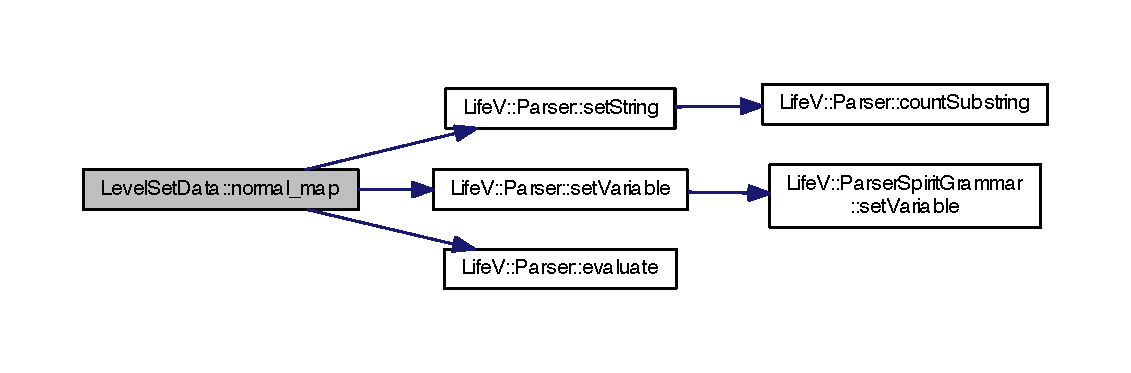
\includegraphics[width=350pt]{classLevelSetData_a674d56690f4e22cbca38bf4b5f176a5e_cgraph}
\end{center}
\end{figure}


\hypertarget{classLevelSetData_ae7f10d3f10b72fbb6f703ba7aa8fe17b}{\index{Level\-Set\-Data@{Level\-Set\-Data}!x\-\_\-map@{x\-\_\-map}}
\index{x\-\_\-map@{x\-\_\-map}!LevelSetData@{Level\-Set\-Data}}
\subsubsection[{x\-\_\-map}]{\setlength{\rightskip}{0pt plus 5cm}scalar\-\_\-type Level\-Set\-Data\-::x\-\_\-map (
\begin{DoxyParamCaption}
\item[{const base\-\_\-node \&}]{t}
\end{DoxyParamCaption}
)}}\label{classLevelSetData_ae7f10d3f10b72fbb6f703ba7aa8fe17b}


Questa funzione rappresenta la mappa dalla frattura piatta, x(t). 


\begin{DoxyCode}
69 \{
70     M\_parser.\hyperlink{classLifeV_1_1Parser_ac05769e836a0dc95d9c020df361a5194}{setString} ( M\_x\_map );
71     M\_parser.\hyperlink{classLifeV_1_1Parser_aa2b362e12b8feb60231705d499c9fbae}{setVariable} ( \textcolor{stringliteral}{"t"}, t [ 0 ] );
72     
73     \textcolor{keywordflow}{return} M\_parser.\hyperlink{classLifeV_1_1Parser_a51d84fd4ae6d420620e7beee58fad673}{evaluate} ();
74 \}
\end{DoxyCode}


Questo è il grafo delle chiamate per questa funzione\-:\nopagebreak
\begin{figure}[H]
\begin{center}
\leavevmode
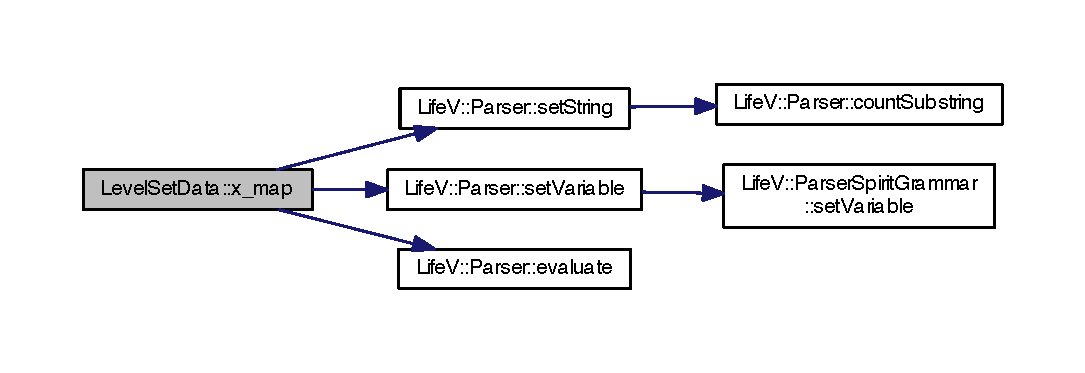
\includegraphics[width=350pt]{classLevelSetData_ae7f10d3f10b72fbb6f703ba7aa8fe17b_cgraph}
\end{center}
\end{figure}


\hypertarget{classLevelSetData_aa4cda1cced4bc385d85383b40bbc2631}{\index{Level\-Set\-Data@{Level\-Set\-Data}!y\-\_\-map@{y\-\_\-map}}
\index{y\-\_\-map@{y\-\_\-map}!LevelSetData@{Level\-Set\-Data}}
\subsubsection[{y\-\_\-map}]{\setlength{\rightskip}{0pt plus 5cm}scalar\-\_\-type Level\-Set\-Data\-::y\-\_\-map (
\begin{DoxyParamCaption}
\item[{const base\-\_\-node \&}]{t}
\end{DoxyParamCaption}
)}}\label{classLevelSetData_aa4cda1cced4bc385d85383b40bbc2631}


Questa funzione rappresenta la mappa dalla frattura piatta, y(t). 


\begin{DoxyCode}
60 \{
61     M\_parser.\hyperlink{classLifeV_1_1Parser_ac05769e836a0dc95d9c020df361a5194}{setString} ( M\_y\_map );
62     M\_parser.\hyperlink{classLifeV_1_1Parser_aa2b362e12b8feb60231705d499c9fbae}{setVariable} ( \textcolor{stringliteral}{"t"}, t [ 0 ] );
63     
64     \textcolor{keywordflow}{return} M\_parser.\hyperlink{classLifeV_1_1Parser_a51d84fd4ae6d420620e7beee58fad673}{evaluate} ();
65 \}
\end{DoxyCode}


Questo è il grafo delle chiamate per questa funzione\-:\nopagebreak
\begin{figure}[H]
\begin{center}
\leavevmode
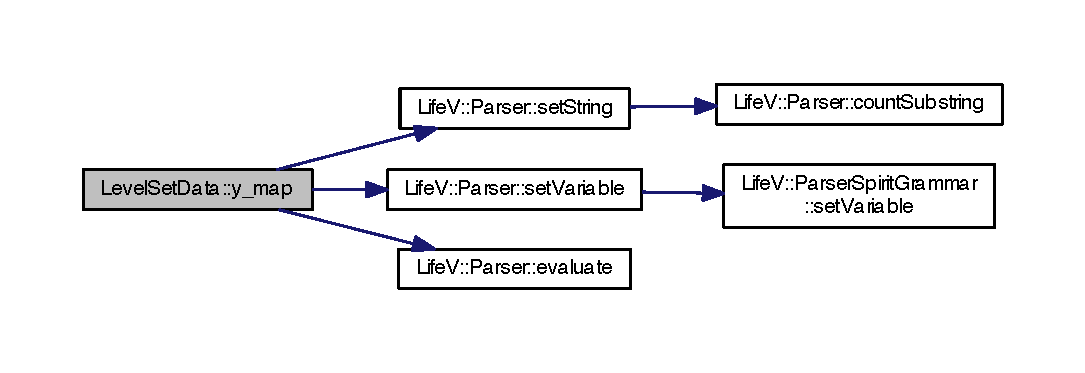
\includegraphics[width=350pt]{classLevelSetData_aa4cda1cced4bc385d85383b40bbc2631_cgraph}
\end{center}
\end{figure}


\hypertarget{classLevelSetData_a732ae59581206d4f94237e54bc0071e3}{\index{Level\-Set\-Data@{Level\-Set\-Data}!ylevel\-Set\-Function@{ylevel\-Set\-Function}}
\index{ylevel\-Set\-Function@{ylevel\-Set\-Function}!LevelSetData@{Level\-Set\-Data}}
\subsubsection[{ylevel\-Set\-Function}]{\setlength{\rightskip}{0pt plus 5cm}scalar\-\_\-type Level\-Set\-Data\-::ylevel\-Set\-Function (
\begin{DoxyParamCaption}
\item[{const base\-\_\-node \&}]{x}
\end{DoxyParamCaption}
)}}\label{classLevelSetData_a732ae59581206d4f94237e54bc0071e3}


Questa funzione definisce il level set che rappresenta la frattura, level set valutato in (x,y). 


\begin{DoxyParams}{Parametri}
{\em base\-\_\-node\&} & x\-: nodo in coordinate ( x, y ) in cui valutare il levelset \\
\hline
\end{DoxyParams}
\begin{DoxyReturn}{Restituisce}
scalar\-\_\-type\-: valore del levelset nel nodo x 
\end{DoxyReturn}

\begin{DoxyCode}
30 \{
31     M\_parser.\hyperlink{classLifeV_1_1Parser_ac05769e836a0dc95d9c020df361a5194}{setString} ( M\_function );
32     M\_parser.\hyperlink{classLifeV_1_1Parser_aa2b362e12b8feb60231705d499c9fbae}{setVariable} ( \textcolor{stringliteral}{"x"}, t [ 0 ] );
33     M\_parser.\hyperlink{classLifeV_1_1Parser_aa2b362e12b8feb60231705d499c9fbae}{setVariable} ( \textcolor{stringliteral}{"y"}, t [ 1 ] );
34     
35     \textcolor{keywordflow}{return} M\_parser.\hyperlink{classLifeV_1_1Parser_a51d84fd4ae6d420620e7beee58fad673}{evaluate} ();
36 \}
\end{DoxyCode}


Questo è il grafo delle chiamate per questa funzione\-:\nopagebreak
\begin{figure}[H]
\begin{center}
\leavevmode
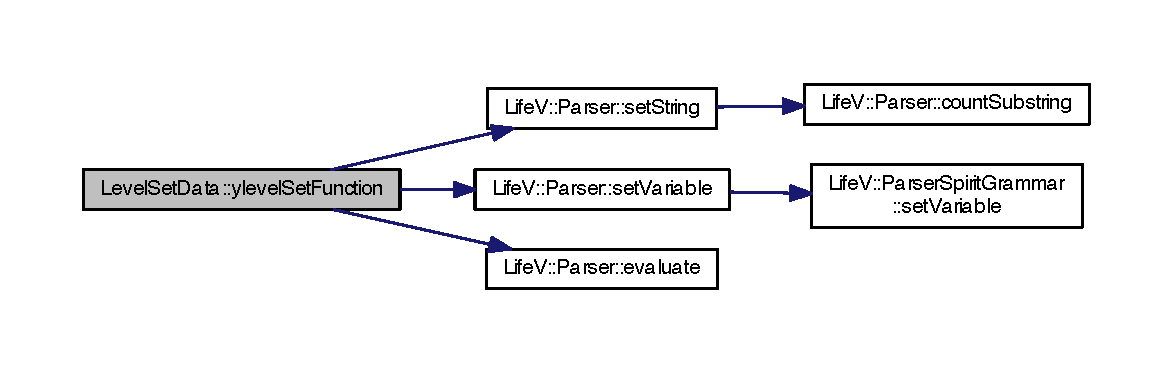
\includegraphics[width=350pt]{classLevelSetData_a732ae59581206d4f94237e54bc0071e3_cgraph}
\end{center}
\end{figure}




La documentazione per questa classe è stata generata a partire dai seguenti file\-:\begin{DoxyCompactItemize}
\item 
include/\hyperlink{LevelSetData_8h}{Level\-Set\-Data.\-h}\item 
src/\hyperlink{LevelSetData_8cc}{Level\-Set\-Data.\-cc}\end{DoxyCompactItemize}

\hypertarget{classLevelSetHandler}{\section{Riferimenti per la classe Level\-Set\-Handler}
\label{classLevelSetHandler}\index{Level\-Set\-Handler@{Level\-Set\-Handler}}
}


\hyperlink{LevelSetHandler_8h}{Level\-Set\-Handler.\-h}.  




{\ttfamily \#include $<$Level\-Set\-Handler.\-h$>$}

\subsection*{Membri pubblici}
\begin{DoxyCompactItemize}
\item 
\hyperlink{classLevelSetHandler_a9dbe142d7d4f677abe8c204714c004ed}{Level\-Set\-Handler} (const Get\-Pot \&data\-File, const std\-::string \&section=\char`\"{}fracture\-Data/\char`\"{}, const std\-::string \&section\-Level\-Set=\char`\"{}level\-Set/\char`\"{})
\begin{DoxyCompactList}\small\item\em \hyperlink{LevelSetHandler_8cc}{Level\-Set\-Handler.\-cc}. \end{DoxyCompactList}\item 
void \hyperlink{classLevelSetHandler_a7ee7ade813923dfdef1bc25e9a881580}{init} (getfem\-::mesh \&medium\-Mesh, const std\-::string \&medium\-Integration\-Type\-Velocity, const getfem\-::mesh\-\_\-fem \&medium\-Mesh\-F\-E\-M\-Pressure, const getfem\-::mesh\-\_\-fem \&medium\-Mesh\-F\-E\-M\-Velocity)
\begin{DoxyCompactList}\small\item\em Funzione che inizializza il level set. \end{DoxyCompactList}\item 
const \hyperlink{Core_8h_a126f7165f04db4ed0b72454469145a08}{G\-F\-Mesh\-Level\-Set\-\_\-\-Type} \& \hyperlink{classLevelSetHandler_a6e08147a60f9e8d7ec65357223f72311}{get\-Mesh} () const 
\item 
\hyperlink{Core_8h_a126f7165f04db4ed0b72454469145a08}{G\-F\-Mesh\-Level\-Set\-\_\-\-Type} \& \hyperlink{classLevelSetHandler_a35e4adb6d0c5128445d46f0b489ce0a2}{get\-Mesh} ()
\item 
const \\*
\hyperlink{Core_8h_ade18ba6e17965b6fdd50b3382b2a7020}{G\-F\-Integration\-Method\-Level\-Set\-\_\-\-Type} \& \hyperlink{classLevelSetHandler_a1bf7aa9bad7c2ccec178d4092690775b}{get\-Integration\-Method\-Inside} () const 
\item 
const \\*
\hyperlink{Core_8h_ade18ba6e17965b6fdd50b3382b2a7020}{G\-F\-Integration\-Method\-Level\-Set\-\_\-\-Type} \& \hyperlink{classLevelSetHandler_a155cedf651006dc5509c34a6ea5e3324}{get\-Integration\-Method\-Outside} () const 
\item 
const \hyperlink{Core_8h_a71358a15bd3925629e26ccbb214a0133}{G\-F\-Level\-Set\-\_\-\-Type} \& \hyperlink{classLevelSetHandler_aa899ffbee62631067378346d61fd172a}{get\-Level\-Set} () const 
\item 
\hyperlink{Core_8h_a71358a15bd3925629e26ccbb214a0133}{G\-F\-Level\-Set\-\_\-\-Type} \& \hyperlink{classLevelSetHandler_a88f16d61da1d2a2a68d5ef33fa77a41d}{get\-Level\-Set} ()
\item 
const \\*
\hyperlink{Core_8h_ade18ba6e17965b6fdd50b3382b2a7020}{G\-F\-Integration\-Method\-Level\-Set\-\_\-\-Type} \& \hyperlink{classLevelSetHandler_ad35aef3284c2582550b376fd3e99c45f}{get\-Integration\-Method} () const 
\item 
const \hyperlink{Core_8h_a4e75b5863535ba1dd79942de2846eff0}{scalar\-Vector\-\_\-\-Type} \& \hyperlink{classLevelSetHandler_a983463087a38199510a0859658ad5291}{get\-Baricenter\-Value} () const 
\item 
const scalar\-\_\-type \& \hyperlink{classLevelSetHandler_a7a4653958485195d2b995be4d52e2765}{get\-Baricenter\-Value} (const size\-\_\-type \&dof) const 
\item 
const \hyperlink{Core_8h_a4e75b5863535ba1dd79942de2846eff0}{scalar\-Vector\-\_\-\-Type} \& \hyperlink{classLevelSetHandler_ac46f075503657b1481d80acb5d3307d1}{get\-D\-O\-F\-Value} () const 
\item 
const scalar\-\_\-type \& \hyperlink{classLevelSetHandler_ab9babfc6e7705047b005a88b4ab1f46f}{get\-D\-O\-F\-Value} (const size\-\_\-type \&dof) const 
\item 
\hyperlink{LevelSetData_8h_a7750f14ec1c622b3c69aa0c5c2894972}{Level\-Set\-Data\-Ptr\-\_\-\-Type} \& \hyperlink{classLevelSetHandler_ab24897cb969210d278f54d94fd8f8977}{get\-Data} ()
\end{DoxyCompactItemize}


\subsection{Descrizione dettagliata}
\hyperlink{LevelSetHandler_8h}{Level\-Set\-Handler.\-h}. 

classe che mi permette di costruire la frattura a partire dai dati del file data 

\subsection{Documentazione dei costruttori e dei distruttori}
\hypertarget{classLevelSetHandler_a9dbe142d7d4f677abe8c204714c004ed}{\index{Level\-Set\-Handler@{Level\-Set\-Handler}!Level\-Set\-Handler@{Level\-Set\-Handler}}
\index{Level\-Set\-Handler@{Level\-Set\-Handler}!LevelSetHandler@{Level\-Set\-Handler}}
\subsubsection[{Level\-Set\-Handler}]{\setlength{\rightskip}{0pt plus 5cm}Level\-Set\-Handler\-::\-Level\-Set\-Handler (
\begin{DoxyParamCaption}
\item[{const Get\-Pot \&}]{data\-File, }
\item[{const std\-::string \&}]{section = {\ttfamily \char`\"{}fractureData/\char`\"{}}, }
\item[{const std\-::string \&}]{section\-Level\-Set = {\ttfamily \char`\"{}levelSet/\char`\"{}}}
\end{DoxyParamCaption}
)}}\label{classLevelSetHandler_a9dbe142d7d4f677abe8c204714c004ed}


\hyperlink{LevelSetHandler_8cc}{Level\-Set\-Handler.\-cc}. 


\begin{DoxyCode}
9                                                                       :
10                                    M\_data( \textcolor{keyword}{new} \hyperlink{classLevelSetData}{LevelSetData\_Type} ( dataFile, section, 
      sectionLevelSet ) )
11 \{\}
\end{DoxyCode}


\subsection{Documentazione delle funzioni membro}
\hypertarget{classLevelSetHandler_a983463087a38199510a0859658ad5291}{\index{Level\-Set\-Handler@{Level\-Set\-Handler}!get\-Baricenter\-Value@{get\-Baricenter\-Value}}
\index{get\-Baricenter\-Value@{get\-Baricenter\-Value}!LevelSetHandler@{Level\-Set\-Handler}}
\subsubsection[{get\-Baricenter\-Value}]{\setlength{\rightskip}{0pt plus 5cm}const {\bf scalar\-Vector\-\_\-\-Type}\& Level\-Set\-Handler\-::get\-Baricenter\-Value (
\begin{DoxyParamCaption}
{}
\end{DoxyParamCaption}
) const\hspace{0.3cm}{\ttfamily [inline]}}}\label{classLevelSetHandler_a983463087a38199510a0859658ad5291}

\begin{DoxyCode}
79     \{
80         \textcolor{keywordflow}{return} M\_baricenterValue;
81     \}
\end{DoxyCode}
\hypertarget{classLevelSetHandler_a7a4653958485195d2b995be4d52e2765}{\index{Level\-Set\-Handler@{Level\-Set\-Handler}!get\-Baricenter\-Value@{get\-Baricenter\-Value}}
\index{get\-Baricenter\-Value@{get\-Baricenter\-Value}!LevelSetHandler@{Level\-Set\-Handler}}
\subsubsection[{get\-Baricenter\-Value}]{\setlength{\rightskip}{0pt plus 5cm}const scalar\-\_\-type\& Level\-Set\-Handler\-::get\-Baricenter\-Value (
\begin{DoxyParamCaption}
\item[{const size\-\_\-type \&}]{dof}
\end{DoxyParamCaption}
) const\hspace{0.3cm}{\ttfamily [inline]}}}\label{classLevelSetHandler_a7a4653958485195d2b995be4d52e2765}

\begin{DoxyCode}
85     \{
86         \textcolor{keywordflow}{return} M\_baricenterValue [ dof ];
87     \}
\end{DoxyCode}
\hypertarget{classLevelSetHandler_ab24897cb969210d278f54d94fd8f8977}{\index{Level\-Set\-Handler@{Level\-Set\-Handler}!get\-Data@{get\-Data}}
\index{get\-Data@{get\-Data}!LevelSetHandler@{Level\-Set\-Handler}}
\subsubsection[{get\-Data}]{\setlength{\rightskip}{0pt plus 5cm}{\bf Level\-Set\-Data\-Ptr\-\_\-\-Type}\& Level\-Set\-Handler\-::get\-Data (
\begin{DoxyParamCaption}
{}
\end{DoxyParamCaption}
)\hspace{0.3cm}{\ttfamily [inline]}}}\label{classLevelSetHandler_ab24897cb969210d278f54d94fd8f8977}

\begin{DoxyCode}
103     \{
104         \textcolor{keywordflow}{return} M\_data;
105     \}
\end{DoxyCode}
\hypertarget{classLevelSetHandler_ac46f075503657b1481d80acb5d3307d1}{\index{Level\-Set\-Handler@{Level\-Set\-Handler}!get\-D\-O\-F\-Value@{get\-D\-O\-F\-Value}}
\index{get\-D\-O\-F\-Value@{get\-D\-O\-F\-Value}!LevelSetHandler@{Level\-Set\-Handler}}
\subsubsection[{get\-D\-O\-F\-Value}]{\setlength{\rightskip}{0pt plus 5cm}const {\bf scalar\-Vector\-\_\-\-Type}\& Level\-Set\-Handler\-::get\-D\-O\-F\-Value (
\begin{DoxyParamCaption}
{}
\end{DoxyParamCaption}
) const\hspace{0.3cm}{\ttfamily [inline]}}}\label{classLevelSetHandler_ac46f075503657b1481d80acb5d3307d1}

\begin{DoxyCode}
91     \{
92         \textcolor{keywordflow}{return} M\_DOFValue;
93     \}
\end{DoxyCode}
\hypertarget{classLevelSetHandler_ab9babfc6e7705047b005a88b4ab1f46f}{\index{Level\-Set\-Handler@{Level\-Set\-Handler}!get\-D\-O\-F\-Value@{get\-D\-O\-F\-Value}}
\index{get\-D\-O\-F\-Value@{get\-D\-O\-F\-Value}!LevelSetHandler@{Level\-Set\-Handler}}
\subsubsection[{get\-D\-O\-F\-Value}]{\setlength{\rightskip}{0pt plus 5cm}const scalar\-\_\-type\& Level\-Set\-Handler\-::get\-D\-O\-F\-Value (
\begin{DoxyParamCaption}
\item[{const size\-\_\-type \&}]{dof}
\end{DoxyParamCaption}
) const\hspace{0.3cm}{\ttfamily [inline]}}}\label{classLevelSetHandler_ab9babfc6e7705047b005a88b4ab1f46f}

\begin{DoxyCode}
97     \{
98         \textcolor{keywordflow}{return} M\_DOFValue [ dof ];
99     \}
\end{DoxyCode}
\hypertarget{classLevelSetHandler_ad35aef3284c2582550b376fd3e99c45f}{\index{Level\-Set\-Handler@{Level\-Set\-Handler}!get\-Integration\-Method@{get\-Integration\-Method}}
\index{get\-Integration\-Method@{get\-Integration\-Method}!LevelSetHandler@{Level\-Set\-Handler}}
\subsubsection[{get\-Integration\-Method}]{\setlength{\rightskip}{0pt plus 5cm}const {\bf G\-F\-Integration\-Method\-Level\-Set\-\_\-\-Type}\& Level\-Set\-Handler\-::get\-Integration\-Method (
\begin{DoxyParamCaption}
{}
\end{DoxyParamCaption}
) const\hspace{0.3cm}{\ttfamily [inline]}}}\label{classLevelSetHandler_ad35aef3284c2582550b376fd3e99c45f}

\begin{DoxyCode}
73     \{
74         \textcolor{keywordflow}{return} *M\_integrationMethod;
75     \}
\end{DoxyCode}
\hypertarget{classLevelSetHandler_a1bf7aa9bad7c2ccec178d4092690775b}{\index{Level\-Set\-Handler@{Level\-Set\-Handler}!get\-Integration\-Method\-Inside@{get\-Integration\-Method\-Inside}}
\index{get\-Integration\-Method\-Inside@{get\-Integration\-Method\-Inside}!LevelSetHandler@{Level\-Set\-Handler}}
\subsubsection[{get\-Integration\-Method\-Inside}]{\setlength{\rightskip}{0pt plus 5cm}const {\bf G\-F\-Integration\-Method\-Level\-Set\-\_\-\-Type}\& Level\-Set\-Handler\-::get\-Integration\-Method\-Inside (
\begin{DoxyParamCaption}
{}
\end{DoxyParamCaption}
) const\hspace{0.3cm}{\ttfamily [inline]}}}\label{classLevelSetHandler_a1bf7aa9bad7c2ccec178d4092690775b}

\begin{DoxyCode}
49     \{
50         \textcolor{keywordflow}{return} *M\_integrationMethodInside;
51     \}
\end{DoxyCode}
\hypertarget{classLevelSetHandler_a155cedf651006dc5509c34a6ea5e3324}{\index{Level\-Set\-Handler@{Level\-Set\-Handler}!get\-Integration\-Method\-Outside@{get\-Integration\-Method\-Outside}}
\index{get\-Integration\-Method\-Outside@{get\-Integration\-Method\-Outside}!LevelSetHandler@{Level\-Set\-Handler}}
\subsubsection[{get\-Integration\-Method\-Outside}]{\setlength{\rightskip}{0pt plus 5cm}const {\bf G\-F\-Integration\-Method\-Level\-Set\-\_\-\-Type}\& Level\-Set\-Handler\-::get\-Integration\-Method\-Outside (
\begin{DoxyParamCaption}
{}
\end{DoxyParamCaption}
) const\hspace{0.3cm}{\ttfamily [inline]}}}\label{classLevelSetHandler_a155cedf651006dc5509c34a6ea5e3324}

\begin{DoxyCode}
55     \{
56         \textcolor{keywordflow}{return} *M\_integrationMethodOutside;
57     \}
\end{DoxyCode}
\hypertarget{classLevelSetHandler_aa899ffbee62631067378346d61fd172a}{\index{Level\-Set\-Handler@{Level\-Set\-Handler}!get\-Level\-Set@{get\-Level\-Set}}
\index{get\-Level\-Set@{get\-Level\-Set}!LevelSetHandler@{Level\-Set\-Handler}}
\subsubsection[{get\-Level\-Set}]{\setlength{\rightskip}{0pt plus 5cm}const {\bf G\-F\-Level\-Set\-\_\-\-Type}\& Level\-Set\-Handler\-::get\-Level\-Set (
\begin{DoxyParamCaption}
{}
\end{DoxyParamCaption}
) const\hspace{0.3cm}{\ttfamily [inline]}}}\label{classLevelSetHandler_aa899ffbee62631067378346d61fd172a}

\begin{DoxyCode}
61     \{
62         \textcolor{keywordflow}{return} *M\_levelSet;
63     \}
\end{DoxyCode}
\hypertarget{classLevelSetHandler_a88f16d61da1d2a2a68d5ef33fa77a41d}{\index{Level\-Set\-Handler@{Level\-Set\-Handler}!get\-Level\-Set@{get\-Level\-Set}}
\index{get\-Level\-Set@{get\-Level\-Set}!LevelSetHandler@{Level\-Set\-Handler}}
\subsubsection[{get\-Level\-Set}]{\setlength{\rightskip}{0pt plus 5cm}{\bf G\-F\-Level\-Set\-\_\-\-Type}\& Level\-Set\-Handler\-::get\-Level\-Set (
\begin{DoxyParamCaption}
{}
\end{DoxyParamCaption}
)\hspace{0.3cm}{\ttfamily [inline]}}}\label{classLevelSetHandler_a88f16d61da1d2a2a68d5ef33fa77a41d}

\begin{DoxyCode}
67     \{
68         \textcolor{keywordflow}{return} *M\_levelSet;
69     \}
\end{DoxyCode}
\hypertarget{classLevelSetHandler_a6e08147a60f9e8d7ec65357223f72311}{\index{Level\-Set\-Handler@{Level\-Set\-Handler}!get\-Mesh@{get\-Mesh}}
\index{get\-Mesh@{get\-Mesh}!LevelSetHandler@{Level\-Set\-Handler}}
\subsubsection[{get\-Mesh}]{\setlength{\rightskip}{0pt plus 5cm}const {\bf G\-F\-Mesh\-Level\-Set\-\_\-\-Type}\& Level\-Set\-Handler\-::get\-Mesh (
\begin{DoxyParamCaption}
{}
\end{DoxyParamCaption}
) const\hspace{0.3cm}{\ttfamily [inline]}}}\label{classLevelSetHandler_a6e08147a60f9e8d7ec65357223f72311}

\begin{DoxyCode}
37     \{
38         \textcolor{keywordflow}{return} *M\_mesh;
39     \}
\end{DoxyCode}
\hypertarget{classLevelSetHandler_a35e4adb6d0c5128445d46f0b489ce0a2}{\index{Level\-Set\-Handler@{Level\-Set\-Handler}!get\-Mesh@{get\-Mesh}}
\index{get\-Mesh@{get\-Mesh}!LevelSetHandler@{Level\-Set\-Handler}}
\subsubsection[{get\-Mesh}]{\setlength{\rightskip}{0pt plus 5cm}{\bf G\-F\-Mesh\-Level\-Set\-\_\-\-Type}\& Level\-Set\-Handler\-::get\-Mesh (
\begin{DoxyParamCaption}
{}
\end{DoxyParamCaption}
)\hspace{0.3cm}{\ttfamily [inline]}}}\label{classLevelSetHandler_a35e4adb6d0c5128445d46f0b489ce0a2}

\begin{DoxyCode}
43     \{
44         \textcolor{keywordflow}{return} *M\_mesh;
45     \}
\end{DoxyCode}
\hypertarget{classLevelSetHandler_a7ee7ade813923dfdef1bc25e9a881580}{\index{Level\-Set\-Handler@{Level\-Set\-Handler}!init@{init}}
\index{init@{init}!LevelSetHandler@{Level\-Set\-Handler}}
\subsubsection[{init}]{\setlength{\rightskip}{0pt plus 5cm}void Level\-Set\-Handler\-::init (
\begin{DoxyParamCaption}
\item[{getfem\-::mesh \&}]{medium\-Mesh, }
\item[{const std\-::string \&}]{medium\-Integration\-Type\-Velocity, }
\item[{const getfem\-::mesh\-\_\-fem \&}]{medium\-Mesh\-F\-E\-M\-Pressure, }
\item[{const getfem\-::mesh\-\_\-fem \&}]{medium\-Mesh\-F\-E\-M\-Velocity}
\end{DoxyParamCaption}
)}}\label{classLevelSetHandler_a7ee7ade813923dfdef1bc25e9a881580}


Funzione che inizializza il level set. 

Partendo dalle informazioni contenute nel file data costrusce le mesh e i metodi di integrazione 
\begin{DoxyParams}{Parametri}
{\em getfem\-::mesh\&} & medium\-Mesh\-: mesh di supporto del mezzo \\
\hline
{\em std\-::string\&} & medium\-Integration\-Type\-Velocity\-: metodo di integrazione per la velocità \\
\hline
{\em getfem\-::mesh\-\_\-fem\&} & medium\-Mesh\-F\-E\-M\-Pressure\-: mesh di integrazione per la pressione \\
\hline
{\em getfem\-::mesh\-\_\-fem\&} & medium\-Mesh\-F\-E\-M\-Velocity\-: mesh di integrazione per la velocità \\
\hline
\end{DoxyParams}

\begin{DoxyCode}
19 \{
20     M\_mesh.reset ( \textcolor{keyword}{new} \hyperlink{Core_8h_a126f7165f04db4ed0b72454469145a08}{GFMeshLevelSet\_Type} ( mediumMesh ) );
21 
22     M\_levelSet.reset ( \textcolor{keyword}{new} \hyperlink{Core_8h_a71358a15bd3925629e26ccbb214a0133}{GFLevelSet\_Type} ( mediumMesh ) );
23 
24     M\_integrationMethod.reset ( \textcolor{keyword}{new} \hyperlink{Core_8h_ade18ba6e17965b6fdd50b3382b2a7020}{GFIntegrationMethodLevelSet\_Type} ( *
      M\_mesh, getfem::mesh\_im\_level\_set::INTEGRATE\_BOUNDARY ) );
25 
26     M\_integrationMethodInside.reset ( \textcolor{keyword}{new} \hyperlink{Core_8h_ade18ba6e17965b6fdd50b3382b2a7020}{GFIntegrationMethodLevelSet\_Type}(
       *M\_mesh, getfem::mesh\_im\_level\_set::INTEGRATE\_INSIDE ) );
27 
28     M\_integrationMethodOutside.reset ( \textcolor{keyword}{new} \hyperlink{Core_8h_ade18ba6e17965b6fdd50b3382b2a7020}{GFIntegrationMethodLevelSet\_Type}
       ( *M\_mesh, getfem::mesh\_im\_level\_set::INTEGRATE\_OUTSIDE ) );
29 
30     \textcolor{comment}{// Level sets}
31 
32     \textcolor{comment}{// Descrizione del metodo di integrazione per la funzione level set}
33     getfem::pintegration\_method integrationType = getfem::int\_method\_descriptor( M\_data->
      getIntegrationTypeSimplex() );
34 
35     \textcolor{comment}{// Definiamo che la M\_mediumMesh M\_levelSetMesh è tagliata da un level set}
36     M\_mesh->add\_level\_set( *M\_levelSet );
37 
38     \textcolor{comment}{// Descrizione del metodo di integrazione per la velocità}
39     getfem::pintegration\_method mediumIntegrationVelocity = getfem::int\_method\_descriptor( 
      mediumIntegrationTypeVelocity );
40 
41     \textcolor{comment}{// Descrizione del metodo di integrazione per la funzione level set di valore zero}
42     M\_integrationMethod->set\_integration\_method ( mediumMesh.convex\_index(), mediumIntegrationVelocity );
43     M\_integrationMethod->set\_simplex\_im ( integrationType );
44 
45     \textcolor{comment}{// Descrizione del metodo di integrazione per un lato della funzione level set}
46     M\_integrationMethodInside->set\_integration\_method ( mediumMesh.convex\_index(), 
      mediumIntegrationVelocity );
47     M\_integrationMethodInside->set\_simplex\_im ( integrationType );
48 
49     \textcolor{comment}{// Descrizione del metodo di integrazione per l'altro lato della funzione level set}
50     M\_integrationMethodOutside->set\_integration\_method ( mediumMesh.convex\_index(), 
      mediumIntegrationVelocity );
51     M\_integrationMethodOutside->set\_simplex\_im ( integrationType );
52 
53     M\_levelSet->reinit();
54     M\_levelSet->values(1) = M\_levelSet->values(0);
55 
56 
57     \textcolor{comment}{// Riempio il level set con i valori nel file data}
58     \textcolor{keywordflow}{for} ( size\_type d = 0; d < M\_levelSet->get\_mesh\_fem().nb\_basic\_dof(); ++d )
59     \{
60         \textcolor{keyword}{const} base\_node node = M\_levelSet->get\_mesh\_fem().point\_of\_basic\_dof(d);
61 
62         M\_levelSet->values(0) [ d ] = M\_data->ylevelSetFunction(node);
63         M\_levelSet->values(1) [ d ] = M\_data->levelSetCutFunction(node);
64     \}
65 
66     M\_levelSet->touch();
67 
68     \textcolor{comment}{// Aggiorno la mesh e i metodi di integrazione poichè il level set è stato modificato}
69     M\_mesh->adapt();
70     M\_integrationMethod->adapt();
71     M\_integrationMethodInside->adapt();
72     M\_integrationMethodOutside->adapt();
73 
74     \textcolor{comment}{// Valuto la funzione level set nei gradi di libertà primari}
75     \textcolor{keyword}{const} size\_type shiftPressure = mediumMeshFEMPressure.nb\_dof();
76     \textcolor{comment}{// gives the total number of different degrees of freedom. If the optional reduction is used, this will
       be the number}
77     \textcolor{comment}{// of columns of the reduction matrix. Otherwise it will return the number of basic degrees of freedom}
78 
79     gmm::resize(M\_baricenterValue, shiftPressure);
80     \textcolor{keywordflow}{for} ( size\_type \hyperlink{matrici_8m_a6f6ccfcf58b31cb6412107d9d5281426}{i} = 0; \hyperlink{matrici_8m_a6f6ccfcf58b31cb6412107d9d5281426}{i} < shiftPressure; ++\hyperlink{matrici_8m_a6f6ccfcf58b31cb6412107d9d5281426}{i} )
81     \{
82         \textcolor{keyword}{const} base\_node node = mediumMeshFEMPressure.point\_of\_basic\_dof ( \hyperlink{matrici_8m_a6f6ccfcf58b31cb6412107d9d5281426}{i} );
83         M\_baricenterValue [ \hyperlink{matrici_8m_a6f6ccfcf58b31cb6412107d9d5281426}{i} ] = M\_data->ylevelSetFunction ( node );
84     \}
85 
86     \textcolor{comment}{// Valuto la funzione level set nei gradi di libertà secondari}
87     \textcolor{keyword}{const} size\_type shiftVelocity = mediumMeshFEMVelocity.nb\_dof();
88     gmm::resize ( M\_DOFValue, shiftVelocity );
89 
90 
91 
92     \textcolor{keywordflow}{for} ( size\_type \hyperlink{matrici_8m_a6f6ccfcf58b31cb6412107d9d5281426}{i} = 0; \hyperlink{matrici_8m_a6f6ccfcf58b31cb6412107d9d5281426}{i} < shiftVelocity; ++\hyperlink{matrici_8m_a6f6ccfcf58b31cb6412107d9d5281426}{i} )
93     \{
94         \textcolor{keyword}{const} base\_node node = mediumMeshFEMVelocity.point\_of\_basic\_dof ( \hyperlink{matrici_8m_a6f6ccfcf58b31cb6412107d9d5281426}{i} );
95         M\_DOFValue [ \hyperlink{matrici_8m_a6f6ccfcf58b31cb6412107d9d5281426}{i} ] = M\_data->ylevelSetFunction ( node );
96     \}
97 
98     \textcolor{keywordflow}{return};
99 \}
\end{DoxyCode}


La documentazione per questa classe è stata generata a partire dai seguenti file\-:\begin{DoxyCompactItemize}
\item 
include/\hyperlink{LevelSetHandler_8h}{Level\-Set\-Handler.\-h}\item 
src/\hyperlink{LevelSetHandler_8cc}{Level\-Set\-Handler.\-cc}\end{DoxyCompactItemize}

\hypertarget{classMatrixBifurcationHandler}{\section{Riferimenti per la classe Matrix\-Bifurcation\-Handler}
\label{classMatrixBifurcationHandler}\index{Matrix\-Bifurcation\-Handler@{Matrix\-Bifurcation\-Handler}}
}


{\ttfamily \#include $<$Matrix\-Bifurcation\-Handler.\-h$>$}

\subsection*{Membri pubblici}
\begin{DoxyCompactItemize}
\item 
\hyperlink{classMatrixBifurcationHandler_a57f9791749acd9b699bf737193c2e87a}{Matrix\-Bifurcation\-Handler} (const Get\-Pot \&data\-File, const std\-::string \&section=\char`\"{}medium\-Data/\char`\"{}, const std\-::string \&subsection=\char`\"{}darcy/\char`\"{})
\begin{DoxyCompactList}\small\item\em Costruttore vuoto di defult. \end{DoxyCompactList}\item 
\hyperlink{classMatrixBifurcationHandler_ad65c01c578ef41e0513e6915cadb068e}{Matrix\-Bifurcation\-Handler} (\hyperlink{Core_8h_a1694976dd66ed00e5f0618f4f8821163}{Matrix2d} \hyperlink{classMatrixBifurcationHandler_ac7d63c6d730079862dd8238928d94b26}{K})
\begin{DoxyCompactList}\small\item\em Costruttore che prende in input la matrice di permeabilità. \end{DoxyCompactList}\item 
\hyperlink{classMatrixBifurcationHandler_a86e7580758aa9a2ec5ef4285e70d06bf}{Matrix\-Bifurcation\-Handler} (scalar\-\_\-type \hyperlink{classMatrixBifurcationHandler_ac7d63c6d730079862dd8238928d94b26}{K})
\begin{DoxyCompactList}\small\item\em Costruttore a partire dalla permeabilità. \end{DoxyCompactList}\item 
void \hyperlink{classMatrixBifurcationHandler_a94433cf28ec2af6ba06b7f63a081d787}{set\-Matrices} (\hyperlink{FractureHandler_8h_a2f0b57e18ecf89912d7de0c87158009e}{Fracture\-Ptr\-Container\-\_\-\-Type} \&fractures)
\begin{DoxyCompactList}\small\item\em Funzione che inizializza M\-\_\-intersection, la classe che rappresenta il triangolo di intersezione, e calcola la matrice T\-\_\- a partire dall'insieme delle fratture che costituiscono l'intersezione. \end{DoxyCompactList}\item 
void \hyperlink{classMatrixBifurcationHandler_aa7e601bac77856cac8db77c58023c1b4}{set\-Triangle} (\hyperlink{classTriangleData}{Triangle\-Data} const \&\hyperlink{classMatrixBifurcationHandler_a3b7305f6106add811e7b4b69f5642e86}{T})
\begin{DoxyCompactList}\small\item\em Funzione che costruisce il triangolo di intersezione a partire da un trangolo già esistente. \end{DoxyCompactList}\item 
void \hyperlink{classMatrixBifurcationHandler_acbc7b99389ad5eacd86f73b0ed08829b}{set\-K} (\hyperlink{Core_8h_a1694976dd66ed00e5f0618f4f8821163}{Matrix2d} \hyperlink{classMatrixBifurcationHandler_ac7d63c6d730079862dd8238928d94b26}{K})
\begin{DoxyCompactList}\small\item\em Funzione che cambia la matrice di permeabilità a partire da una matrice data. \end{DoxyCompactList}\item 
\hyperlink{Core_8h_a1694976dd66ed00e5f0618f4f8821163}{Matrix2d} \hyperlink{classMatrixBifurcationHandler_ac7d63c6d730079862dd8238928d94b26}{K} () const 
\begin{DoxyCompactList}\small\item\em Funzione che restituisce la matrice di permeabilità. \end{DoxyCompactList}\item 
void \hyperlink{classMatrixBifurcationHandler_ac134a5731e6614e543241a018ccf8c34}{compute\-N} ()
\begin{DoxyCompactList}\small\item\em Funzione che calcola la matrice N\-\_\-, matrice che ha per righe le normali ai lati. \end{DoxyCompactList}\item 
\hyperlink{Core_8h_aee82131e398edee47a44d675ee802368}{Matrix32} \hyperlink{classMatrixBifurcationHandler_a77f006579fad0f0f08c10bf684bbd16a}{N} () const 
\begin{DoxyCompactList}\small\item\em Funzione che restituisce la matrice N\-\_\-, matrice che ha per righe le normali ai lati. \end{DoxyCompactList}\item 
void \hyperlink{classMatrixBifurcationHandler_ac179ca406307a3d2ee5d5b5af94d265e}{compute\-C} ()
\begin{DoxyCompactList}\small\item\em Funzione che calcola la matrice C\-\_\-, matrice che ha per righe i vettori che uniscono il baricentro del triangolo con il punto medio di ogni lato. \end{DoxyCompactList}\item 
\hyperlink{Core_8h_aee82131e398edee47a44d675ee802368}{Matrix32} \hyperlink{classMatrixBifurcationHandler_a4701fef8d864cb7d61521c8fbe5db2cc}{C} ()
\begin{DoxyCompactList}\small\item\em Funzione che restituisce la matrice C\-\_\-, matrice che ha per righe i vettori che uniscono il baricentro del triangolo con il punto medio di ogni lato. \end{DoxyCompactList}\item 
void \hyperlink{classMatrixBifurcationHandler_a203b6bfcdef418ffa927aebaeedc6da2}{compute\-Qc} ()
\begin{DoxyCompactList}\small\item\em Funzione che costruisce la matrice Qc\-\_\-, matrice che ha per colonne una base ortonormale per la matrice trasposta di C. \end{DoxyCompactList}\item 
\hyperlink{Core_8h_aee82131e398edee47a44d675ee802368}{Matrix32} \hyperlink{classMatrixBifurcationHandler_add50b813d3bd773ddf794c4e05b37e38}{Qc} () const 
\begin{DoxyCompactList}\small\item\em Funzione che restituisce la matrice Qc\-\_\-, matrice che ha per colonne una base ortonormale per la matrice trasposta di C. \end{DoxyCompactList}\item 
\hyperlink{Core_8h_acd816705c6602062b91975525c4e3f6f}{Matrix3d} \hyperlink{classMatrixBifurcationHandler_ad84675e9be6d56de69c0e25bf1cd77cd}{Pc} () const 
\begin{DoxyCompactList}\small\item\em Funzione che restituisce la matrice Pc\-\_\-, matrice di proiezione sullo spazio nullo di Qc\-\_\-. \end{DoxyCompactList}\item 
void \hyperlink{classMatrixBifurcationHandler_a46ee3c60eedda32abe36700ab2ce2d16}{compute\-T} (scalar\-\_\-type t=6.\-0)
\begin{DoxyCompactList}\small\item\em Funzione che calcola la matrice T\-\_\-, matrice di trasmissibilità. \end{DoxyCompactList}\item 
void \hyperlink{classMatrixBifurcationHandler_a2153adb36bdbba82ca18ae74eb9e2ea7}{compute\-Tsimple} (scalar\-\_\-type t=6.\-0)
\item 
void \hyperlink{classMatrixBifurcationHandler_acafb7a17c3d639068938a21dad6bb0ec}{inversion2\-X2} (const \hyperlink{Core_8h_a1694976dd66ed00e5f0618f4f8821163}{Matrix2d} \&invk, scalar\-\_\-type det)
\item 
\hyperlink{classMatrixBifurcationHandler}{Matrix\-Bifurcation\-Handler} \& \hyperlink{classMatrixBifurcationHandler_a2d67172a5034f104d08cb53e5dbda926}{operator=} (const \hyperlink{classMatrixBifurcationHandler}{Matrix\-Bifurcation\-Handler} \&mat)
\item 
\hyperlink{Core_8h_acd816705c6602062b91975525c4e3f6f}{Matrix3d} \hyperlink{classMatrixBifurcationHandler_a3b7305f6106add811e7b4b69f5642e86}{T} () const 
\end{DoxyCompactItemize}


\subsection{Documentazione dei costruttori e dei distruttori}
\hypertarget{classMatrixBifurcationHandler_a57f9791749acd9b699bf737193c2e87a}{\index{Matrix\-Bifurcation\-Handler@{Matrix\-Bifurcation\-Handler}!Matrix\-Bifurcation\-Handler@{Matrix\-Bifurcation\-Handler}}
\index{Matrix\-Bifurcation\-Handler@{Matrix\-Bifurcation\-Handler}!MatrixBifurcationHandler@{Matrix\-Bifurcation\-Handler}}
\subsubsection[{Matrix\-Bifurcation\-Handler}]{\setlength{\rightskip}{0pt plus 5cm}Matrix\-Bifurcation\-Handler\-::\-Matrix\-Bifurcation\-Handler (
\begin{DoxyParamCaption}
\item[{const Get\-Pot \&}]{data\-File, }
\item[{const std\-::string \&}]{section = {\ttfamily \char`\"{}mediumData/\char`\"{}}, }
\item[{const std\-::string \&}]{subsection = {\ttfamily \char`\"{}darcy/\char`\"{}}}
\end{DoxyParamCaption}
)}}\label{classMatrixBifurcationHandler_a57f9791749acd9b699bf737193c2e87a}


Costruttore vuoto di defult. 

Definisce la matrice 3x3 Pc\-\_\- costante pari a 1/3 e riempie la matrice 2x2 K\-\_\-, leggendo dal file \char`\"{}data\char`\"{} 
\begin{DoxyParams}{Parametri}
{\em Get\-Pot\&} & data\-File\-: nome del file data da cui leggere i dati \\
\hline
{\em std\-::string\&} & section = \char`\"{}medium\-Data/\char`\"{}\-: nome della sezione nel file data in cui leggere, se non è fornita è posta di default pari a \char`\"{}medium\-Data/\char`\"{} \\
\hline
{\em std\-::string\&} & subsection = \char`\"{}darcy/\char`\"{}\-: nome della sottosezione nel file data in cui leggere, se non è fornita è posta di default pari a \char`\"{}darcy/\char`\"{} \\
\hline
\end{DoxyParams}

\begin{DoxyCode}
6                                                                                 :Pc\_(Matrix3d::Constant(1./
      3.0))
7 \{
8     \hyperlink{Core_8h_a1694976dd66ed00e5f0618f4f8821163}{Matrix2d} invk; 
9     scalar\_type det = dataFile ( (section + subsection + \textcolor{stringliteral}{"invK"}).data(), 1. );
10     
11     invk(0,0) = dataFile ( ( section + subsection + \textcolor{stringliteral}{"invKDist11"} ).data (), 1. );
12     invk(0,1) = dataFile ( ( section + subsection + \textcolor{stringliteral}{"invKDist12"} ).data (), 0. );
13     invk(1,0) = dataFile ( ( section + subsection + \textcolor{stringliteral}{"invKDist12"} ).data (), 0. );
14     invk(1,1) = dataFile ( ( section + subsection + \textcolor{stringliteral}{"invKDist22"} ).data (), 1. );
15     
16     
17     this-> \hyperlink{classMatrixBifurcationHandler_acafb7a17c3d639068938a21dad6bb0ec}{inversion2X2} ( invk, det );
18     
19 \}\textcolor{comment}{// costruttore}
\end{DoxyCode}
\hypertarget{classMatrixBifurcationHandler_ad65c01c578ef41e0513e6915cadb068e}{\index{Matrix\-Bifurcation\-Handler@{Matrix\-Bifurcation\-Handler}!Matrix\-Bifurcation\-Handler@{Matrix\-Bifurcation\-Handler}}
\index{Matrix\-Bifurcation\-Handler@{Matrix\-Bifurcation\-Handler}!MatrixBifurcationHandler@{Matrix\-Bifurcation\-Handler}}
\subsubsection[{Matrix\-Bifurcation\-Handler}]{\setlength{\rightskip}{0pt plus 5cm}Matrix\-Bifurcation\-Handler\-::\-Matrix\-Bifurcation\-Handler (
\begin{DoxyParamCaption}
\item[{{\bf Matrix2d}}]{K}
\end{DoxyParamCaption}
)}}\label{classMatrixBifurcationHandler_ad65c01c578ef41e0513e6915cadb068e}


Costruttore che prende in input la matrice di permeabilità. 

Definisce la matrice 3x3 Pc\-\_\- costante pari a 1/3 e riempie la matrice 2x2 K\-\_\- usando la matrice K fornita. 
\begin{DoxyParams}{Parametri}
{\em Matrix2d} & K\-: matrice di permeabilità da usare per modificare K\-\_\- \\
\hline
\end{DoxyParams}

\begin{DoxyCode}
29 :K\_(\hyperlink{classMatrixBifurcationHandler_ac7d63c6d730079862dd8238928d94b26}{K}),Pc\_(Matrix3d::Constant(1./3.0))\{\};
\end{DoxyCode}
\hypertarget{classMatrixBifurcationHandler_a86e7580758aa9a2ec5ef4285e70d06bf}{\index{Matrix\-Bifurcation\-Handler@{Matrix\-Bifurcation\-Handler}!Matrix\-Bifurcation\-Handler@{Matrix\-Bifurcation\-Handler}}
\index{Matrix\-Bifurcation\-Handler@{Matrix\-Bifurcation\-Handler}!MatrixBifurcationHandler@{Matrix\-Bifurcation\-Handler}}
\subsubsection[{Matrix\-Bifurcation\-Handler}]{\setlength{\rightskip}{0pt plus 5cm}Matrix\-Bifurcation\-Handler\-::\-Matrix\-Bifurcation\-Handler (
\begin{DoxyParamCaption}
\item[{scalar\-\_\-type}]{K}
\end{DoxyParamCaption}
)\hspace{0.3cm}{\ttfamily [explicit]}}}\label{classMatrixBifurcationHandler_a86e7580758aa9a2ec5ef4285e70d06bf}


Costruttore a partire dalla permeabilità. 

Definisce la matrice 3x3 Pc\-\_\- costante pari a 1/3 e riempie la matrice 2x2 K\-\_\- usando lo scalare K, inizializzandola come una matrice con K sulla diagonale e 0 fuori. 
\begin{DoxyCode}
22                                                                :Pc\_(Matrix3d::Constant(1./3.0))
23 \{
24     K\_(0,0)=\hyperlink{classMatrixBifurcationHandler_ac7d63c6d730079862dd8238928d94b26}{K};
25     K\_(0,1)=K\_(1,0)=0.0;
26     K\_(1,1)=\hyperlink{classMatrixBifurcationHandler_ac7d63c6d730079862dd8238928d94b26}{K};
27 \}\textcolor{comment}{// costruttore}
\end{DoxyCode}


\subsection{Documentazione delle funzioni membro}
\hypertarget{classMatrixBifurcationHandler_a4701fef8d864cb7d61521c8fbe5db2cc}{\index{Matrix\-Bifurcation\-Handler@{Matrix\-Bifurcation\-Handler}!C@{C}}
\index{C@{C}!MatrixBifurcationHandler@{Matrix\-Bifurcation\-Handler}}
\subsubsection[{C}]{\setlength{\rightskip}{0pt plus 5cm}{\bf Matrix32} Matrix\-Bifurcation\-Handler\-::\-C (
\begin{DoxyParamCaption}
{}
\end{DoxyParamCaption}
)\hspace{0.3cm}{\ttfamily [inline]}}}\label{classMatrixBifurcationHandler_a4701fef8d864cb7d61521c8fbe5db2cc}


Funzione che restituisce la matrice C\-\_\-, matrice che ha per righe i vettori che uniscono il baricentro del triangolo con il punto medio di ogni lato. 

\begin{DoxyReturn}{Restituisce}
Matrix32 C\-\_\-\-: matrice 3x2 
\end{DoxyReturn}

\begin{DoxyCode}
113 \{\textcolor{keywordflow}{return} C\_;\}
\end{DoxyCode}
\hypertarget{classMatrixBifurcationHandler_ac179ca406307a3d2ee5d5b5af94d265e}{\index{Matrix\-Bifurcation\-Handler@{Matrix\-Bifurcation\-Handler}!compute\-C@{compute\-C}}
\index{compute\-C@{compute\-C}!MatrixBifurcationHandler@{Matrix\-Bifurcation\-Handler}}
\subsubsection[{compute\-C}]{\setlength{\rightskip}{0pt plus 5cm}void Matrix\-Bifurcation\-Handler\-::compute\-C (
\begin{DoxyParamCaption}
{}
\end{DoxyParamCaption}
)}}\label{classMatrixBifurcationHandler_ac179ca406307a3d2ee5d5b5af94d265e}


Funzione che calcola la matrice C\-\_\-, matrice che ha per righe i vettori che uniscono il baricentro del triangolo con il punto medio di ogni lato. 

Ovviamente per poter chiamare questo metodo è necessario che il triangolo che rappresenta l'intersezione sia stato già definito. 
\begin{DoxyCode}
48 \{
49     C\_.row(0) = M\_intersection.\hyperlink{classIntersection_a603d1cb4b33762c72999968ceec95a39}{intersectionTriangle} ().\hyperlink{classTriangleData_a4278f62058529df47e095421d02599ad}{c}(0).transpose();
50     C\_.row(1) = M\_intersection.\hyperlink{classIntersection_a603d1cb4b33762c72999968ceec95a39}{intersectionTriangle} ().\hyperlink{classTriangleData_a4278f62058529df47e095421d02599ad}{c}(1).transpose();
51     C\_.row(2) = M\_intersection.\hyperlink{classIntersection_a603d1cb4b33762c72999968ceec95a39}{intersectionTriangle} ().\hyperlink{classTriangleData_a4278f62058529df47e095421d02599ad}{c}(2).transpose();
52 \}\textcolor{comment}{// computeC}
\end{DoxyCode}
\hypertarget{classMatrixBifurcationHandler_ac134a5731e6614e543241a018ccf8c34}{\index{Matrix\-Bifurcation\-Handler@{Matrix\-Bifurcation\-Handler}!compute\-N@{compute\-N}}
\index{compute\-N@{compute\-N}!MatrixBifurcationHandler@{Matrix\-Bifurcation\-Handler}}
\subsubsection[{compute\-N}]{\setlength{\rightskip}{0pt plus 5cm}void Matrix\-Bifurcation\-Handler\-::compute\-N (
\begin{DoxyParamCaption}
{}
\end{DoxyParamCaption}
)}}\label{classMatrixBifurcationHandler_ac134a5731e6614e543241a018ccf8c34}


Funzione che calcola la matrice N\-\_\-, matrice che ha per righe le normali ai lati. 

Ovviamente per poter chiamare questo metodo è necessario che il triangolo che rappresenta l'intersezione sia stato già definito. 
\begin{DoxyCode}
41 \{
42     N\_.row(0)=M\_intersection.\hyperlink{classIntersection_a603d1cb4b33762c72999968ceec95a39}{intersectionTriangle} ().
      \hyperlink{classTriangleData_a3b110e4ceb09cc5368fcecad9938a1c8}{unscaledNormal}(0).transpose();
43     N\_.row(1)=M\_intersection.\hyperlink{classIntersection_a603d1cb4b33762c72999968ceec95a39}{intersectionTriangle} ().
      \hyperlink{classTriangleData_a3b110e4ceb09cc5368fcecad9938a1c8}{unscaledNormal}(1).transpose();
44     N\_.row(2)=M\_intersection.\hyperlink{classIntersection_a603d1cb4b33762c72999968ceec95a39}{intersectionTriangle} ().
      \hyperlink{classTriangleData_a3b110e4ceb09cc5368fcecad9938a1c8}{unscaledNormal}(2).transpose();
45 \}\textcolor{comment}{// computeN}
\end{DoxyCode}
\hypertarget{classMatrixBifurcationHandler_a203b6bfcdef418ffa927aebaeedc6da2}{\index{Matrix\-Bifurcation\-Handler@{Matrix\-Bifurcation\-Handler}!compute\-Qc@{compute\-Qc}}
\index{compute\-Qc@{compute\-Qc}!MatrixBifurcationHandler@{Matrix\-Bifurcation\-Handler}}
\subsubsection[{compute\-Qc}]{\setlength{\rightskip}{0pt plus 5cm}void Matrix\-Bifurcation\-Handler\-::compute\-Qc (
\begin{DoxyParamCaption}
{}
\end{DoxyParamCaption}
)}}\label{classMatrixBifurcationHandler_a203b6bfcdef418ffa927aebaeedc6da2}


Funzione che costruisce la matrice Qc\-\_\-, matrice che ha per colonne una base ortonormale per la matrice trasposta di C. 

La funzione richiama il calcolo di C\-\_\-, quindi non è necessario che sia stata precedentemente calcolata. 
\begin{DoxyCode}
56 \{
57     this->\hyperlink{classMatrixBifurcationHandler_ac179ca406307a3d2ee5d5b5af94d265e}{computeC}();
58     Qc\_.col(0)  = C\_.col(0).normalized();
59     \hyperlink{Core_8h_aab1614cfe385b1f15b9ce723bacfaec9}{Vector3d} v0 = Qc\_.col(0);
60     \hyperlink{Core_8h_aab1614cfe385b1f15b9ce723bacfaec9}{Vector3d} v1 = C\_.col(1) - ( v0.dot(C\_.col(1)) )*v0;
61     Qc\_.col(1)  = v1.normalized();
62 \}\textcolor{comment}{// computeQc}
\end{DoxyCode}
\hypertarget{classMatrixBifurcationHandler_a46ee3c60eedda32abe36700ab2ce2d16}{\index{Matrix\-Bifurcation\-Handler@{Matrix\-Bifurcation\-Handler}!compute\-T@{compute\-T}}
\index{compute\-T@{compute\-T}!MatrixBifurcationHandler@{Matrix\-Bifurcation\-Handler}}
\subsubsection[{compute\-T}]{\setlength{\rightskip}{0pt plus 5cm}void Matrix\-Bifurcation\-Handler\-::compute\-T (
\begin{DoxyParamCaption}
\item[{scalar\-\_\-type}]{t = {\ttfamily 6.0}}
\end{DoxyParamCaption}
)}}\label{classMatrixBifurcationHandler_a46ee3c60eedda32abe36700ab2ce2d16}


Funzione che calcola la matrice T\-\_\-, matrice di trasmissibilità. 

La matrice T\-\_\- deriva dall'applicazione di uno schema alle differenze finite mimetiche sul triangolo di intersezione per la legge di Darcy, ignorando l'effetto della gravità. Questa funzione richiama il calcolo delle matrici C\-\_\-, N\-\_\- e Qc\-\_\-. L'approssimazione di T\-\_\- assume la seguente forma\-: T= N K N$^\wedge$\-T + t \{trace\}(N\-K\-N$^\wedge$\-T)P\-\_\-c 
\begin{DoxyCode}
66 \{
67     this->\hyperlink{classMatrixBifurcationHandler_a203b6bfcdef418ffa927aebaeedc6da2}{computeQc}();
68     this->\hyperlink{classMatrixBifurcationHandler_ac134a5731e6614e543241a018ccf8c34}{computeN}();
69 
70     scalar\_type area = M\_intersection.\hyperlink{classIntersection_a603d1cb4b33762c72999968ceec95a39}{intersectionTriangle} ().
      \hyperlink{classTriangleData_acbfbc62d5221ecd37437012fe8b68c8d}{measure}();
71     \hyperlink{Core_8h_acd816705c6602062b91975525c4e3f6f}{Matrix3d} Nkn = N\_*K\_*N\_.transpose();
72     
73     Eigen::DiagonalMatrix<scalar\_type,3,3> Nd (Nkn.diagonal());
74     
75     \hyperlink{Core_8h_acd816705c6602062b91975525c4e3f6f}{Matrix3d} tmp = Pc\_ *Nd *Pc\_;
76     
77     T\_=(1./area)*( Nkn + t*tmp );
78 \}\textcolor{comment}{// computeT}
\end{DoxyCode}
\hypertarget{classMatrixBifurcationHandler_a2153adb36bdbba82ca18ae74eb9e2ea7}{\index{Matrix\-Bifurcation\-Handler@{Matrix\-Bifurcation\-Handler}!compute\-Tsimple@{compute\-Tsimple}}
\index{compute\-Tsimple@{compute\-Tsimple}!MatrixBifurcationHandler@{Matrix\-Bifurcation\-Handler}}
\subsubsection[{compute\-Tsimple}]{\setlength{\rightskip}{0pt plus 5cm}void Matrix\-Bifurcation\-Handler\-::compute\-Tsimple (
\begin{DoxyParamCaption}
\item[{scalar\-\_\-type}]{t = {\ttfamily 6.0}}
\end{DoxyParamCaption}
)}}\label{classMatrixBifurcationHandler_a2153adb36bdbba82ca18ae74eb9e2ea7}

\begin{DoxyCode}
82 \{
83     this->\hyperlink{classMatrixBifurcationHandler_a203b6bfcdef418ffa927aebaeedc6da2}{computeQc}();
84     this->\hyperlink{classMatrixBifurcationHandler_ac134a5731e6614e543241a018ccf8c34}{computeN}();
85 
86     scalar\_type area = M\_intersection.\hyperlink{classIntersection_a603d1cb4b33762c72999968ceec95a39}{intersectionTriangle} ().
      \hyperlink{classTriangleData_acbfbc62d5221ecd37437012fe8b68c8d}{measure}();
87     \hyperlink{Core_8h_acd816705c6602062b91975525c4e3f6f}{Matrix3d} Nkn = N\_*K\_*N\_.transpose();
88     
89     scalar\_type Nd=Nkn.trace();
90     
91     \hyperlink{Core_8h_acd816705c6602062b91975525c4e3f6f}{Matrix3d} tmp = Nd *Pc\_;
92     
93     T\_=(1./area)*( Nkn + t*tmp );
94 \}\textcolor{comment}{// computeTsimple}
\end{DoxyCode}
\hypertarget{classMatrixBifurcationHandler_acafb7a17c3d639068938a21dad6bb0ec}{\index{Matrix\-Bifurcation\-Handler@{Matrix\-Bifurcation\-Handler}!inversion2\-X2@{inversion2\-X2}}
\index{inversion2\-X2@{inversion2\-X2}!MatrixBifurcationHandler@{Matrix\-Bifurcation\-Handler}}
\subsubsection[{inversion2\-X2}]{\setlength{\rightskip}{0pt plus 5cm}void Matrix\-Bifurcation\-Handler\-::inversion2\-X2 (
\begin{DoxyParamCaption}
\item[{const {\bf Matrix2d} \&}]{invk, }
\item[{scalar\-\_\-type}]{det}
\end{DoxyParamCaption}
)}}\label{classMatrixBifurcationHandler_acafb7a17c3d639068938a21dad6bb0ec}

\begin{DoxyCode}
98 \{
99     this-> K\_ ( 0, 0 ) = invk ( 1, 1 )*1./det;
100     this-> K\_ ( 0, 1 ) = -invk ( 0, 1 )*1./det;
101     this-> K\_ ( 1, 0 ) = -invk ( 1, 0 )*1./det;
102     this-> K\_ ( 1, 1 ) = invk ( 0, 0 )*1./det;
103 \}\textcolor{comment}{// inversion2X2}
\end{DoxyCode}
\hypertarget{classMatrixBifurcationHandler_ac7d63c6d730079862dd8238928d94b26}{\index{Matrix\-Bifurcation\-Handler@{Matrix\-Bifurcation\-Handler}!K@{K}}
\index{K@{K}!MatrixBifurcationHandler@{Matrix\-Bifurcation\-Handler}}
\subsubsection[{K}]{\setlength{\rightskip}{0pt plus 5cm}{\bf Matrix2d} Matrix\-Bifurcation\-Handler\-::\-K (
\begin{DoxyParamCaption}
{}
\end{DoxyParamCaption}
) const\hspace{0.3cm}{\ttfamily [inline]}}}\label{classMatrixBifurcationHandler_ac7d63c6d730079862dd8238928d94b26}


Funzione che restituisce la matrice di permeabilità. 

\begin{DoxyReturn}{Restituisce}
Matrix2d K\-\_\-\-: matrice di permeabilità 
\end{DoxyReturn}

\begin{DoxyCode}
82 \{ \textcolor{keywordflow}{return} K\_;\}
\end{DoxyCode}
\hypertarget{classMatrixBifurcationHandler_a77f006579fad0f0f08c10bf684bbd16a}{\index{Matrix\-Bifurcation\-Handler@{Matrix\-Bifurcation\-Handler}!N@{N}}
\index{N@{N}!MatrixBifurcationHandler@{Matrix\-Bifurcation\-Handler}}
\subsubsection[{N}]{\setlength{\rightskip}{0pt plus 5cm}{\bf Matrix32} Matrix\-Bifurcation\-Handler\-::\-N (
\begin{DoxyParamCaption}
{}
\end{DoxyParamCaption}
) const\hspace{0.3cm}{\ttfamily [inline]}}}\label{classMatrixBifurcationHandler_a77f006579fad0f0f08c10bf684bbd16a}


Funzione che restituisce la matrice N\-\_\-, matrice che ha per righe le normali ai lati. 

\begin{DoxyReturn}{Restituisce}
Matrix32 N\-\_\-\-: matrice 3x2 
\end{DoxyReturn}

\begin{DoxyCode}
96 \{\textcolor{keywordflow}{return} N\_;\}
\end{DoxyCode}
\hypertarget{classMatrixBifurcationHandler_a2d67172a5034f104d08cb53e5dbda926}{\index{Matrix\-Bifurcation\-Handler@{Matrix\-Bifurcation\-Handler}!operator=@{operator=}}
\index{operator=@{operator=}!MatrixBifurcationHandler@{Matrix\-Bifurcation\-Handler}}
\subsubsection[{operator=}]{\setlength{\rightskip}{0pt plus 5cm}{\bf Matrix\-Bifurcation\-Handler}\& Matrix\-Bifurcation\-Handler\-::operator= (
\begin{DoxyParamCaption}
\item[{const {\bf Matrix\-Bifurcation\-Handler} \&}]{mat}
\end{DoxyParamCaption}
)\hspace{0.3cm}{\ttfamily [inline]}}}\label{classMatrixBifurcationHandler_a2d67172a5034f104d08cb53e5dbda926}

\begin{DoxyCode}
154     \{
155         M\_intersection = mat.M\_intersection;
156         K\_ = mat.K\_;
157         N\_ = mat.N\_;
158         C\_ = mat.C\_;
159         Qc\_ = mat.Qc\_;
160         Pc\_ = mat.Pc\_;
161         T\_ = mat.T\_;
162     \}
\end{DoxyCode}
\hypertarget{classMatrixBifurcationHandler_ad84675e9be6d56de69c0e25bf1cd77cd}{\index{Matrix\-Bifurcation\-Handler@{Matrix\-Bifurcation\-Handler}!Pc@{Pc}}
\index{Pc@{Pc}!MatrixBifurcationHandler@{Matrix\-Bifurcation\-Handler}}
\subsubsection[{Pc}]{\setlength{\rightskip}{0pt plus 5cm}{\bf Matrix3d} Matrix\-Bifurcation\-Handler\-::\-Pc (
\begin{DoxyParamCaption}
{}
\end{DoxyParamCaption}
) const\hspace{0.3cm}{\ttfamily [inline]}}}\label{classMatrixBifurcationHandler_ad84675e9be6d56de69c0e25bf1cd77cd}


Funzione che restituisce la matrice Pc\-\_\-, matrice di proiezione sullo spazio nullo di Qc\-\_\-. 

\begin{DoxyReturn}{Restituisce}
Matrix3d Pc\-\_\-\-: matrice 3x3 
\end{DoxyReturn}

\begin{DoxyCode}
134 \{ \textcolor{keywordflow}{return} Pc\_; \}
\end{DoxyCode}
\hypertarget{classMatrixBifurcationHandler_add50b813d3bd773ddf794c4e05b37e38}{\index{Matrix\-Bifurcation\-Handler@{Matrix\-Bifurcation\-Handler}!Qc@{Qc}}
\index{Qc@{Qc}!MatrixBifurcationHandler@{Matrix\-Bifurcation\-Handler}}
\subsubsection[{Qc}]{\setlength{\rightskip}{0pt plus 5cm}{\bf Matrix32} Matrix\-Bifurcation\-Handler\-::\-Qc (
\begin{DoxyParamCaption}
{}
\end{DoxyParamCaption}
) const\hspace{0.3cm}{\ttfamily [inline]}}}\label{classMatrixBifurcationHandler_add50b813d3bd773ddf794c4e05b37e38}


Funzione che restituisce la matrice Qc\-\_\-, matrice che ha per colonne una base ortonormale per la matrice trasposta di C. 

\begin{DoxyReturn}{Restituisce}
Matrix32 Qc\-\_\-\-: matrice 3x2 
\end{DoxyReturn}

\begin{DoxyCode}
127 \{ \textcolor{keywordflow}{return} Qc\_; \}
\end{DoxyCode}
\hypertarget{classMatrixBifurcationHandler_acbc7b99389ad5eacd86f73b0ed08829b}{\index{Matrix\-Bifurcation\-Handler@{Matrix\-Bifurcation\-Handler}!set\-K@{set\-K}}
\index{set\-K@{set\-K}!MatrixBifurcationHandler@{Matrix\-Bifurcation\-Handler}}
\subsubsection[{set\-K}]{\setlength{\rightskip}{0pt plus 5cm}void Matrix\-Bifurcation\-Handler\-::set\-K (
\begin{DoxyParamCaption}
\item[{{\bf Matrix2d}}]{K}
\end{DoxyParamCaption}
)\hspace{0.3cm}{\ttfamily [inline]}}}\label{classMatrixBifurcationHandler_acbc7b99389ad5eacd86f73b0ed08829b}


Funzione che cambia la matrice di permeabilità a partire da una matrice data. 


\begin{DoxyParams}{Parametri}
{\em Matrix2d} & K\-: matrice di permeabilità da sostituire \\
\hline
\end{DoxyParams}

\begin{DoxyCode}
75 \{K\_=\hyperlink{classMatrixBifurcationHandler_ac7d63c6d730079862dd8238928d94b26}{K};\}
\end{DoxyCode}
\hypertarget{classMatrixBifurcationHandler_a94433cf28ec2af6ba06b7f63a081d787}{\index{Matrix\-Bifurcation\-Handler@{Matrix\-Bifurcation\-Handler}!set\-Matrices@{set\-Matrices}}
\index{set\-Matrices@{set\-Matrices}!MatrixBifurcationHandler@{Matrix\-Bifurcation\-Handler}}
\subsubsection[{set\-Matrices}]{\setlength{\rightskip}{0pt plus 5cm}void Matrix\-Bifurcation\-Handler\-::set\-Matrices (
\begin{DoxyParamCaption}
\item[{{\bf Fracture\-Ptr\-Container\-\_\-\-Type} \&}]{fractures}
\end{DoxyParamCaption}
)}}\label{classMatrixBifurcationHandler_a94433cf28ec2af6ba06b7f63a081d787}


Funzione che inizializza M\-\_\-intersection, la classe che rappresenta il triangolo di intersezione, e calcola la matrice T\-\_\- a partire dall'insieme delle fratture che costituiscono l'intersezione. 


\begin{DoxyParams}{Parametri}
{\em Fracture\-Ptr\-Container\-\_\-\-Type\&} & fractures\-: vettore delle fratture che costituiscono l'intersezione \\
\hline
\end{DoxyParams}

\begin{DoxyCode}
33 \{
34     M\_intersection.\hyperlink{classIntersection_a6694ead6072e98dffe4a7c70379ca83b}{setIntersection} ( fractures );
35     
36     \hyperlink{classMatrixBifurcationHandler_a46ee3c60eedda32abe36700ab2ce2d16}{computeT}(); 
37 \}\textcolor{comment}{// setMatrices}
\end{DoxyCode}
\hypertarget{classMatrixBifurcationHandler_aa7e601bac77856cac8db77c58023c1b4}{\index{Matrix\-Bifurcation\-Handler@{Matrix\-Bifurcation\-Handler}!set\-Triangle@{set\-Triangle}}
\index{set\-Triangle@{set\-Triangle}!MatrixBifurcationHandler@{Matrix\-Bifurcation\-Handler}}
\subsubsection[{set\-Triangle}]{\setlength{\rightskip}{0pt plus 5cm}void Matrix\-Bifurcation\-Handler\-::set\-Triangle (
\begin{DoxyParamCaption}
\item[{{\bf Triangle\-Data} const \&}]{T}
\end{DoxyParamCaption}
)\hspace{0.3cm}{\ttfamily [inline]}}}\label{classMatrixBifurcationHandler_aa7e601bac77856cac8db77c58023c1b4}


Funzione che costruisce il triangolo di intersezione a partire da un trangolo già esistente. 


\begin{DoxyParams}{Parametri}
{\em \hyperlink{classTriangleData}{Triangle\-Data}} & const \& T\-: triangolo già esistente da cui partire per costruire l'intersezione \\
\hline
\end{DoxyParams}

\begin{DoxyCode}
66     \{
67         M\_intersection.\hyperlink{classIntersection_ae071ecb3d3f2d6f9723e310764535883}{setTriangle} ( \hyperlink{classMatrixBifurcationHandler_a3b7305f6106add811e7b4b69f5642e86}{T} );
68     \}
\end{DoxyCode}
\hypertarget{classMatrixBifurcationHandler_a3b7305f6106add811e7b4b69f5642e86}{\index{Matrix\-Bifurcation\-Handler@{Matrix\-Bifurcation\-Handler}!T@{T}}
\index{T@{T}!MatrixBifurcationHandler@{Matrix\-Bifurcation\-Handler}}
\subsubsection[{T}]{\setlength{\rightskip}{0pt plus 5cm}{\bf Matrix3d} Matrix\-Bifurcation\-Handler\-::\-T (
\begin{DoxyParamCaption}
{}
\end{DoxyParamCaption}
) const\hspace{0.3cm}{\ttfamily [inline]}}}\label{classMatrixBifurcationHandler_a3b7305f6106add811e7b4b69f5642e86}

\begin{DoxyCode}
165 \{\textcolor{keywordflow}{return} T\_;\}
\end{DoxyCode}


La documentazione per questa classe è stata generata a partire dai seguenti file\-:\begin{DoxyCompactItemize}
\item 
include/\hyperlink{MatrixBifurcationHandler_8h}{Matrix\-Bifurcation\-Handler.\-h}\item 
src/\hyperlink{MatrixBifurcationHandler_8cc}{Matrix\-Bifurcation\-Handler.\-cc}\end{DoxyCompactItemize}

\hypertarget{classMediumData}{\section{Riferimenti per la classe Medium\-Data}
\label{classMediumData}\index{Medium\-Data@{Medium\-Data}}
}


\hyperlink{MediumData_8h}{Medium\-Data.\-h}.  




{\ttfamily \#include $<$Medium\-Data.\-h$>$}

\subsection*{Membri pubblici}
\begin{DoxyCompactItemize}
\item 
\hyperlink{classMediumData_aff5b247e34c08dbfa373e4cde5118da2}{Medium\-Data} (const Get\-Pot \&data\-File, const std\-::string \&section\-Solver, const std\-::string \&section=\char`\"{}medium\-Data/\char`\"{}, const std\-::string \&section\-Domain=\char`\"{}domain/\char`\"{})
\begin{DoxyCompactList}\small\item\em \hyperlink{MediumData_8cc}{Medium\-Data.\-cc}. \end{DoxyCompactList}\item 
scalar\-\_\-type \hyperlink{classMediumData_a41b88e8b0d9eb57c51e7aad518867ff1}{exact} (const base\-\_\-node \&x, const scalar\-\_\-type \&t=0) const 
\begin{DoxyCompactList}\small\item\em funzione che valuta la soluzione esatta in un dato nodo \end{DoxyCompactList}\item 
scalar\-\_\-type \hyperlink{classMediumData_adc228cb9d834aae8886ec520093a003a}{exact\-Outlet} (const base\-\_\-node \&x, const scalar\-\_\-type \&t=0) const 
\begin{DoxyCompactList}\small\item\em funzione che valuta la soluzione esatta in un dato nodo nella regione in cui level set $>$ 0 \end{DoxyCompactList}\item 
scalar\-\_\-type \hyperlink{classMediumData_a9e2ebf4af56f981be28836750fd58a17}{exact\-Inlet} (const base\-\_\-node \&x, const scalar\-\_\-type \&t=0) const 
\begin{DoxyCompactList}\small\item\em funzione che valuta la soluzione esatta in un dato nodo nella regione in cui level set $<$ 0 \end{DoxyCompactList}\item 
scalar\-\_\-type \hyperlink{classMediumData_a6f3d3b64009602eb22a7c54b74a33a34}{exact\-Flux} (const base\-\_\-node \&x, const base\-\_\-node \&n, const scalar\-\_\-type \&t=0) const 
\begin{DoxyCompactList}\small\item\em funzione che valuta il flusso esatto in un dato nodo \end{DoxyCompactList}\item 
scalar\-\_\-type \hyperlink{classMediumData_a1f5a2647becdcd8db8ad4c1a9b79b29e}{source} (const base\-\_\-node \&x, const scalar\-\_\-type \&t=0) const 
\begin{DoxyCompactList}\small\item\em funzione che valuta il termine sorgente in un dato nodo \end{DoxyCompactList}\item 
scalar\-\_\-type \hyperlink{classMediumData_aae75c00abbad84594130890eb34dafd9}{inv\-K\-Distribution11} (const base\-\_\-node \&x) const 
\begin{DoxyCompactList}\small\item\em funzione che restituisce un'eventuale modulazione del coefficiente di permeabilità \end{DoxyCompactList}\item 
scalar\-\_\-type \hyperlink{classMediumData_aef29ca88f4183c72f590abffcff1fc87}{inv\-K\-Distribution12} (const base\-\_\-node \&x) const 
\begin{DoxyCompactList}\small\item\em funzione che restituisce un'eventuale modulazione del coefficiente di permeabilità \end{DoxyCompactList}\item 
scalar\-\_\-type \hyperlink{classMediumData_a5298eacbba56d9f3d6bc6b2297cdac31}{inv\-K\-Distribution22} (const base\-\_\-node \&x) const 
\begin{DoxyCompactList}\small\item\em funzione che restituisce un'eventuale modulazione del coefficiente di permeabilità \end{DoxyCompactList}\item 
scalar\-\_\-type \hyperlink{classMediumData_a80235292e1223f4b68a37832f7be9828}{exact\-Initial} (const base\-\_\-node \&x) const 
\item 
scalar\-\_\-type \hyperlink{classMediumData_a72374c5da3834b4313280f5ae53406fb}{get\-Inv\-K} () const 
\item 
scalar\-\_\-type \hyperlink{classMediumData_ac1646aa22f5ed8ea92a14560dfc0905f}{get\-Penalty\-Vector} () const 
\item 
scalar\-\_\-type \hyperlink{classMediumData_a627f26f5f80bb4139a548e2d2cce1a47}{get\-Penalty\-Scalar} () const 
\end{DoxyCompactItemize}


\subsection{Descrizione dettagliata}
\hyperlink{MediumData_8h}{Medium\-Data.\-h}. 

classe che contiene le informazioni sulle proprietà del mezzo e sui metodi di integrazione 

\subsection{Documentazione dei costruttori e dei distruttori}
\hypertarget{classMediumData_aff5b247e34c08dbfa373e4cde5118da2}{\index{Medium\-Data@{Medium\-Data}!Medium\-Data@{Medium\-Data}}
\index{Medium\-Data@{Medium\-Data}!MediumData@{Medium\-Data}}
\subsubsection[{Medium\-Data}]{\setlength{\rightskip}{0pt plus 5cm}Medium\-Data\-::\-Medium\-Data (
\begin{DoxyParamCaption}
\item[{const Get\-Pot \&}]{data\-File, }
\item[{const std\-::string \&}]{section\-Solver, }
\item[{const std\-::string \&}]{section = {\ttfamily \char`\"{}mediumData/\char`\"{}}, }
\item[{const std\-::string \&}]{section\-Domain = {\ttfamily \char`\"{}domain/\char`\"{}}}
\end{DoxyParamCaption}
)}}\label{classMediumData_aff5b247e34c08dbfa373e4cde5118da2}


\hyperlink{MediumData_8cc}{Medium\-Data.\-cc}. 


\begin{DoxyParams}{Parametri}
{\em data\-File} & variabile di tipo Get\-Pot che contiene il nome del file data \\
\hline
{\em section} & nome della sezione corrispondente al mezzo \\
\hline
{\em section\-Domain} & noe della sezione del mezzo corrispondente alle caratteristiche del dominio\\
\hline
\end{DoxyParams}

\begin{DoxyCode}
12                                                           :
13             M\_section( section ),
14             M\_sectionDomain( M\_section + sectionDomain ),
15             M\_sectionSolver( M\_section + sectionSolver ),
16             M\_penaltyVector( dataFile ( ( M\_sectionDomain + \textcolor{stringliteral}{"penaltyVelocity"} ).data(), 5. ) ),
17             M\_penaltyScalar( dataFile ( ( M\_sectionDomain + \textcolor{stringliteral}{"penaltyPressure"} ).data(), 1. ) ),
18             \textcolor{comment}{// darcy }
19             M\_invK( dataFile ( ( M\_sectionSolver + \textcolor{stringliteral}{"invK"} ).data(), 1. ) ),
20             M\_invKDistribution11( dataFile ( ( M\_sectionSolver + \textcolor{stringliteral}{"invKDist11"} ).data(), \textcolor{stringliteral}{"1."} ) ),
21             M\_invKDistribution12( dataFile ( ( M\_sectionSolver + \textcolor{stringliteral}{"invKDist12"} ).data(), \textcolor{stringliteral}{"1."} ) ),
22             M\_invKDistribution22( dataFile ( ( M\_sectionSolver + \textcolor{stringliteral}{"invKDist22"} ).data(), \textcolor{stringliteral}{"1."} ) ),
23             M\_exact(dataFile( ( M\_sectionSolver + \textcolor{stringliteral}{"solution"} ).data(), \textcolor{stringliteral}{"x"} ) ),
24             M\_exactInlet( dataFile ( ( M\_sectionSolver + \textcolor{stringliteral}{"solutionIn"} ).data(), M\_exact.data() ) ), 
25             M\_exactOutlet( dataFile ( ( M\_sectionSolver + \textcolor{stringliteral}{"solutionOut"} ).data(), M\_exact.data() ) ), 
26             M\_exactFlux( dataFile ( ( M\_sectionSolver + \textcolor{stringliteral}{"velocity"} ).data(), \textcolor{stringliteral}{"1."} ) ),
27             M\_source(dataFile( ( M\_sectionSolver + \textcolor{stringliteral}{"source"} ).data(), \textcolor{stringliteral}{"1."} ) ),
28             M\_exactInitial( dataFile ( ( M\_sectionSolver + \textcolor{stringliteral}{"initialCondition"} ).data(), \textcolor{stringliteral}{"0."} ) )
29 \{
30 \}\textcolor{comment}{// costruttore}
\end{DoxyCode}


\subsection{Documentazione delle funzioni membro}
\hypertarget{classMediumData_a41b88e8b0d9eb57c51e7aad518867ff1}{\index{Medium\-Data@{Medium\-Data}!exact@{exact}}
\index{exact@{exact}!MediumData@{Medium\-Data}}
\subsubsection[{exact}]{\setlength{\rightskip}{0pt plus 5cm}scalar\-\_\-type Medium\-Data\-::exact (
\begin{DoxyParamCaption}
\item[{const base\-\_\-node \&}]{x, }
\item[{const scalar\-\_\-type \&}]{t = {\ttfamily 0}}
\end{DoxyParamCaption}
) const}}\label{classMediumData_a41b88e8b0d9eb57c51e7aad518867ff1}


funzione che valuta la soluzione esatta in un dato nodo 


\begin{DoxyParams}{Parametri}
{\em x} & bgeot\-::base\-\_\-node, nodo geometrico \\
\hline
\end{DoxyParams}

\begin{DoxyCode}
35 \{
36     M\_parser.\hyperlink{classLifeV_1_1Parser_ac05769e836a0dc95d9c020df361a5194}{setString}(M\_exact);
37 
38     M\_parser.\hyperlink{classLifeV_1_1Parser_aa2b362e12b8feb60231705d499c9fbae}{setVariable}(\textcolor{stringliteral}{"x"}, x [ 0 ]);
39     M\_parser.\hyperlink{classLifeV_1_1Parser_aa2b362e12b8feb60231705d499c9fbae}{setVariable}(\textcolor{stringliteral}{"y"}, x [ 1 ]);
40     M\_parser.\hyperlink{classLifeV_1_1Parser_aa2b362e12b8feb60231705d499c9fbae}{setVariable}(\textcolor{stringliteral}{"t"}, t);
41 
42     \textcolor{keywordflow}{return} M\_parser.\hyperlink{classLifeV_1_1Parser_a51d84fd4ae6d420620e7beee58fad673}{evaluate}();
43 \}\textcolor{comment}{// exact}
\end{DoxyCode}
\hypertarget{classMediumData_a6f3d3b64009602eb22a7c54b74a33a34}{\index{Medium\-Data@{Medium\-Data}!exact\-Flux@{exact\-Flux}}
\index{exact\-Flux@{exact\-Flux}!MediumData@{Medium\-Data}}
\subsubsection[{exact\-Flux}]{\setlength{\rightskip}{0pt plus 5cm}scalar\-\_\-type Medium\-Data\-::exact\-Flux (
\begin{DoxyParamCaption}
\item[{const base\-\_\-node \&}]{x, }
\item[{const base\-\_\-node \&}]{n, }
\item[{const scalar\-\_\-type \&}]{t = {\ttfamily 0}}
\end{DoxyParamCaption}
) const}}\label{classMediumData_a6f3d3b64009602eb22a7c54b74a33a34}


funzione che valuta il flusso esatto in un dato nodo 


\begin{DoxyParams}{Parametri}
{\em x} & bgeot\-::base\-\_\-node, nodo geometrico \\
\hline
{\em n} & bgeot\-::base\-\_\-node, vettore normale \\
\hline
\end{DoxyParams}

\begin{DoxyCode}
76 \{
77     M\_parser.\hyperlink{classLifeV_1_1Parser_ac05769e836a0dc95d9c020df361a5194}{setString}(M\_exactFlux);
78 
79     M\_parser.\hyperlink{classLifeV_1_1Parser_aa2b362e12b8feb60231705d499c9fbae}{setVariable}(\textcolor{stringliteral}{"x"}, x [ 0 ]);
80     M\_parser.\hyperlink{classLifeV_1_1Parser_aa2b362e12b8feb60231705d499c9fbae}{setVariable}(\textcolor{stringliteral}{"y"}, x [ 1 ]);
81     M\_parser.\hyperlink{classLifeV_1_1Parser_aa2b362e12b8feb60231705d499c9fbae}{setVariable}(\textcolor{stringliteral}{"n1"}, n [ 0 ]);
82     M\_parser.\hyperlink{classLifeV_1_1Parser_aa2b362e12b8feb60231705d499c9fbae}{setVariable}(\textcolor{stringliteral}{"n2"}, n [ 1 ]);
83     M\_parser.\hyperlink{classLifeV_1_1Parser_aa2b362e12b8feb60231705d499c9fbae}{setVariable}(\textcolor{stringliteral}{"t"}, t);
84 
85     \textcolor{keywordflow}{return} M\_parser.\hyperlink{classLifeV_1_1Parser_a51d84fd4ae6d420620e7beee58fad673}{evaluate}();
86 \}\textcolor{comment}{// exactFlux}
\end{DoxyCode}
\hypertarget{classMediumData_a80235292e1223f4b68a37832f7be9828}{\index{Medium\-Data@{Medium\-Data}!exact\-Initial@{exact\-Initial}}
\index{exact\-Initial@{exact\-Initial}!MediumData@{Medium\-Data}}
\subsubsection[{exact\-Initial}]{\setlength{\rightskip}{0pt plus 5cm}scalar\-\_\-type Medium\-Data\-::exact\-Initial (
\begin{DoxyParamCaption}
\item[{const base\-\_\-node \&}]{x}
\end{DoxyParamCaption}
) const}}\label{classMediumData_a80235292e1223f4b68a37832f7be9828}

\begin{DoxyCode}
139 \{
140     M\_parser.\hyperlink{classLifeV_1_1Parser_ac05769e836a0dc95d9c020df361a5194}{setString}(M\_exactInitial);
141 
142     M\_parser.\hyperlink{classLifeV_1_1Parser_aa2b362e12b8feb60231705d499c9fbae}{setVariable}(\textcolor{stringliteral}{"x"}, x [ 0 ]);
143     M\_parser.\hyperlink{classLifeV_1_1Parser_aa2b362e12b8feb60231705d499c9fbae}{setVariable}(\textcolor{stringliteral}{"y"}, x [ 1 ]);
144 
145     \textcolor{keywordflow}{return} M\_parser.\hyperlink{classLifeV_1_1Parser_a51d84fd4ae6d420620e7beee58fad673}{evaluate}();
146 \}\textcolor{comment}{// exactInitial}
\end{DoxyCode}
\hypertarget{classMediumData_a9e2ebf4af56f981be28836750fd58a17}{\index{Medium\-Data@{Medium\-Data}!exact\-Inlet@{exact\-Inlet}}
\index{exact\-Inlet@{exact\-Inlet}!MediumData@{Medium\-Data}}
\subsubsection[{exact\-Inlet}]{\setlength{\rightskip}{0pt plus 5cm}scalar\-\_\-type Medium\-Data\-::exact\-Inlet (
\begin{DoxyParamCaption}
\item[{const base\-\_\-node \&}]{x, }
\item[{const scalar\-\_\-type \&}]{t = {\ttfamily 0}}
\end{DoxyParamCaption}
) const}}\label{classMediumData_a9e2ebf4af56f981be28836750fd58a17}


funzione che valuta la soluzione esatta in un dato nodo nella regione in cui level set $<$ 0 


\begin{DoxyParams}{Parametri}
{\em x} & bgeot\-::base\-\_\-node, nodo geometrico \\
\hline
\end{DoxyParams}

\begin{DoxyCode}
48 \{
49     M\_parser.\hyperlink{classLifeV_1_1Parser_ac05769e836a0dc95d9c020df361a5194}{setString}(M\_exactInlet);
50 
51     M\_parser.\hyperlink{classLifeV_1_1Parser_aa2b362e12b8feb60231705d499c9fbae}{setVariable}(\textcolor{stringliteral}{"x"}, x [ 0 ]);
52     M\_parser.\hyperlink{classLifeV_1_1Parser_aa2b362e12b8feb60231705d499c9fbae}{setVariable}(\textcolor{stringliteral}{"y"}, x [ 1 ]);
53     M\_parser.\hyperlink{classLifeV_1_1Parser_aa2b362e12b8feb60231705d499c9fbae}{setVariable}(\textcolor{stringliteral}{"t"}, t);
54 
55     \textcolor{keywordflow}{return} M\_parser.\hyperlink{classLifeV_1_1Parser_a51d84fd4ae6d420620e7beee58fad673}{evaluate}();
56 \}\textcolor{comment}{// exactInlet}
\end{DoxyCode}
\hypertarget{classMediumData_adc228cb9d834aae8886ec520093a003a}{\index{Medium\-Data@{Medium\-Data}!exact\-Outlet@{exact\-Outlet}}
\index{exact\-Outlet@{exact\-Outlet}!MediumData@{Medium\-Data}}
\subsubsection[{exact\-Outlet}]{\setlength{\rightskip}{0pt plus 5cm}scalar\-\_\-type Medium\-Data\-::exact\-Outlet (
\begin{DoxyParamCaption}
\item[{const base\-\_\-node \&}]{x, }
\item[{const scalar\-\_\-type \&}]{t = {\ttfamily 0}}
\end{DoxyParamCaption}
) const}}\label{classMediumData_adc228cb9d834aae8886ec520093a003a}


funzione che valuta la soluzione esatta in un dato nodo nella regione in cui level set $>$ 0 


\begin{DoxyParams}{Parametri}
{\em x} & bgeot\-::base\-\_\-node, nodo geometrico \\
\hline
\end{DoxyParams}

\begin{DoxyCode}
61 \{
62     M\_parser.\hyperlink{classLifeV_1_1Parser_ac05769e836a0dc95d9c020df361a5194}{setString}(M\_exactOutlet);
63 
64     M\_parser.\hyperlink{classLifeV_1_1Parser_aa2b362e12b8feb60231705d499c9fbae}{setVariable}(\textcolor{stringliteral}{"x"}, x [ 0 ]);
65     M\_parser.\hyperlink{classLifeV_1_1Parser_aa2b362e12b8feb60231705d499c9fbae}{setVariable}(\textcolor{stringliteral}{"y"}, x [ 1 ]);
66     M\_parser.\hyperlink{classLifeV_1_1Parser_aa2b362e12b8feb60231705d499c9fbae}{setVariable}(\textcolor{stringliteral}{"t"}, t);
67 
68     \textcolor{keywordflow}{return} M\_parser.\hyperlink{classLifeV_1_1Parser_a51d84fd4ae6d420620e7beee58fad673}{evaluate}();
69 \}\textcolor{comment}{// exactOutlet}
\end{DoxyCode}
\hypertarget{classMediumData_a72374c5da3834b4313280f5ae53406fb}{\index{Medium\-Data@{Medium\-Data}!get\-Inv\-K@{get\-Inv\-K}}
\index{get\-Inv\-K@{get\-Inv\-K}!MediumData@{Medium\-Data}}
\subsubsection[{get\-Inv\-K}]{\setlength{\rightskip}{0pt plus 5cm}scalar\-\_\-type Medium\-Data\-::get\-Inv\-K (
\begin{DoxyParamCaption}
{}
\end{DoxyParamCaption}
) const\hspace{0.3cm}{\ttfamily [inline]}}}\label{classMediumData_a72374c5da3834b4313280f5ae53406fb}

\begin{DoxyCode}
96     \{
97         \textcolor{keywordflow}{return} M\_invK;
98     \}
\end{DoxyCode}
\hypertarget{classMediumData_a627f26f5f80bb4139a548e2d2cce1a47}{\index{Medium\-Data@{Medium\-Data}!get\-Penalty\-Scalar@{get\-Penalty\-Scalar}}
\index{get\-Penalty\-Scalar@{get\-Penalty\-Scalar}!MediumData@{Medium\-Data}}
\subsubsection[{get\-Penalty\-Scalar}]{\setlength{\rightskip}{0pt plus 5cm}scalar\-\_\-type Medium\-Data\-::get\-Penalty\-Scalar (
\begin{DoxyParamCaption}
{}
\end{DoxyParamCaption}
) const\hspace{0.3cm}{\ttfamily [inline]}}}\label{classMediumData_a627f26f5f80bb4139a548e2d2cce1a47}

\begin{DoxyCode}
108     \{
109         \textcolor{keywordflow}{return} M\_penaltyScalar;
110     \}
\end{DoxyCode}
\hypertarget{classMediumData_ac1646aa22f5ed8ea92a14560dfc0905f}{\index{Medium\-Data@{Medium\-Data}!get\-Penalty\-Vector@{get\-Penalty\-Vector}}
\index{get\-Penalty\-Vector@{get\-Penalty\-Vector}!MediumData@{Medium\-Data}}
\subsubsection[{get\-Penalty\-Vector}]{\setlength{\rightskip}{0pt plus 5cm}scalar\-\_\-type Medium\-Data\-::get\-Penalty\-Vector (
\begin{DoxyParamCaption}
{}
\end{DoxyParamCaption}
) const\hspace{0.3cm}{\ttfamily [inline]}}}\label{classMediumData_ac1646aa22f5ed8ea92a14560dfc0905f}

\begin{DoxyCode}
102     \{
103         \textcolor{keywordflow}{return} M\_penaltyVector;
104     \}
\end{DoxyCode}
\hypertarget{classMediumData_aae75c00abbad84594130890eb34dafd9}{\index{Medium\-Data@{Medium\-Data}!inv\-K\-Distribution11@{inv\-K\-Distribution11}}
\index{inv\-K\-Distribution11@{inv\-K\-Distribution11}!MediumData@{Medium\-Data}}
\subsubsection[{inv\-K\-Distribution11}]{\setlength{\rightskip}{0pt plus 5cm}scalar\-\_\-type Medium\-Data\-::inv\-K\-Distribution11 (
\begin{DoxyParamCaption}
\item[{const base\-\_\-node \&}]{x}
\end{DoxyParamCaption}
) const}}\label{classMediumData_aae75c00abbad84594130890eb34dafd9}


funzione che restituisce un'eventuale modulazione del coefficiente di permeabilità 


\begin{DoxyParams}{Parametri}
{\em x} & bgeot\-::base\-\_\-node, nodo geometrico \\
\hline
\end{DoxyParams}

\begin{DoxyCode}
103 \{
104     M\_parser.\hyperlink{classLifeV_1_1Parser_ac05769e836a0dc95d9c020df361a5194}{setString}(M\_invKDistribution11);
105 
106     M\_parser.\hyperlink{classLifeV_1_1Parser_aa2b362e12b8feb60231705d499c9fbae}{setVariable}(\textcolor{stringliteral}{"x"}, x [ 0 ]);
107     M\_parser.\hyperlink{classLifeV_1_1Parser_aa2b362e12b8feb60231705d499c9fbae}{setVariable}(\textcolor{stringliteral}{"y"}, x [ 1 ]);
108 
109     \textcolor{keywordflow}{return} M\_parser.\hyperlink{classLifeV_1_1Parser_a51d84fd4ae6d420620e7beee58fad673}{evaluate}();
110 \}\textcolor{comment}{// invKDistribution11}
\end{DoxyCode}
\hypertarget{classMediumData_aef29ca88f4183c72f590abffcff1fc87}{\index{Medium\-Data@{Medium\-Data}!inv\-K\-Distribution12@{inv\-K\-Distribution12}}
\index{inv\-K\-Distribution12@{inv\-K\-Distribution12}!MediumData@{Medium\-Data}}
\subsubsection[{inv\-K\-Distribution12}]{\setlength{\rightskip}{0pt plus 5cm}scalar\-\_\-type Medium\-Data\-::inv\-K\-Distribution12 (
\begin{DoxyParamCaption}
\item[{const base\-\_\-node \&}]{x}
\end{DoxyParamCaption}
) const}}\label{classMediumData_aef29ca88f4183c72f590abffcff1fc87}


funzione che restituisce un'eventuale modulazione del coefficiente di permeabilità 


\begin{DoxyParams}{Parametri}
{\em x} & bgeot\-::base\-\_\-node, nodo geometrico \\
\hline
\end{DoxyParams}

\begin{DoxyCode}
115 \{
116     M\_parser.\hyperlink{classLifeV_1_1Parser_ac05769e836a0dc95d9c020df361a5194}{setString}(M\_invKDistribution12);
117 
118     M\_parser.\hyperlink{classLifeV_1_1Parser_aa2b362e12b8feb60231705d499c9fbae}{setVariable}(\textcolor{stringliteral}{"x"}, x [ 0 ]);
119     M\_parser.\hyperlink{classLifeV_1_1Parser_aa2b362e12b8feb60231705d499c9fbae}{setVariable}(\textcolor{stringliteral}{"y"}, x [ 1 ]);
120 
121     \textcolor{keywordflow}{return} M\_parser.\hyperlink{classLifeV_1_1Parser_a51d84fd4ae6d420620e7beee58fad673}{evaluate}();
122 \}\textcolor{comment}{// invKDistribution12}
\end{DoxyCode}
\hypertarget{classMediumData_a5298eacbba56d9f3d6bc6b2297cdac31}{\index{Medium\-Data@{Medium\-Data}!inv\-K\-Distribution22@{inv\-K\-Distribution22}}
\index{inv\-K\-Distribution22@{inv\-K\-Distribution22}!MediumData@{Medium\-Data}}
\subsubsection[{inv\-K\-Distribution22}]{\setlength{\rightskip}{0pt plus 5cm}scalar\-\_\-type Medium\-Data\-::inv\-K\-Distribution22 (
\begin{DoxyParamCaption}
\item[{const base\-\_\-node \&}]{x}
\end{DoxyParamCaption}
) const}}\label{classMediumData_a5298eacbba56d9f3d6bc6b2297cdac31}


funzione che restituisce un'eventuale modulazione del coefficiente di permeabilità 


\begin{DoxyParams}{Parametri}
{\em x} & bgeot\-::base\-\_\-node, nodo geometrico \\
\hline
\end{DoxyParams}

\begin{DoxyCode}
127 \{
128     M\_parser.\hyperlink{classLifeV_1_1Parser_ac05769e836a0dc95d9c020df361a5194}{setString}(M\_invKDistribution22);
129 
130     M\_parser.\hyperlink{classLifeV_1_1Parser_aa2b362e12b8feb60231705d499c9fbae}{setVariable}(\textcolor{stringliteral}{"x"}, x [ 0 ]);
131     M\_parser.\hyperlink{classLifeV_1_1Parser_aa2b362e12b8feb60231705d499c9fbae}{setVariable}(\textcolor{stringliteral}{"y"}, x [ 1 ]);
132 
133     \textcolor{keywordflow}{return} M\_parser.\hyperlink{classLifeV_1_1Parser_a51d84fd4ae6d420620e7beee58fad673}{evaluate}();
134 \}\textcolor{comment}{// invKDistribution22}
\end{DoxyCode}
\hypertarget{classMediumData_a1f5a2647becdcd8db8ad4c1a9b79b29e}{\index{Medium\-Data@{Medium\-Data}!source@{source}}
\index{source@{source}!MediumData@{Medium\-Data}}
\subsubsection[{source}]{\setlength{\rightskip}{0pt plus 5cm}scalar\-\_\-type Medium\-Data\-::source (
\begin{DoxyParamCaption}
\item[{const base\-\_\-node \&}]{x, }
\item[{const scalar\-\_\-type \&}]{t = {\ttfamily 0}}
\end{DoxyParamCaption}
) const}}\label{classMediumData_a1f5a2647becdcd8db8ad4c1a9b79b29e}


funzione che valuta il termine sorgente in un dato nodo 


\begin{DoxyParams}{Parametri}
{\em x} & bgeot\-::base\-\_\-node, nodo geometrico \\
\hline
\end{DoxyParams}

\begin{DoxyCode}
91 \{
92     M\_parser.\hyperlink{classLifeV_1_1Parser_ac05769e836a0dc95d9c020df361a5194}{setString}(M\_source);
93 
94     M\_parser.\hyperlink{classLifeV_1_1Parser_aa2b362e12b8feb60231705d499c9fbae}{setVariable}(\textcolor{stringliteral}{"x"}, x [ 0 ]);
95     M\_parser.\hyperlink{classLifeV_1_1Parser_aa2b362e12b8feb60231705d499c9fbae}{setVariable}(\textcolor{stringliteral}{"y"}, x [ 1 ]);
96     M\_parser.\hyperlink{classLifeV_1_1Parser_aa2b362e12b8feb60231705d499c9fbae}{setVariable}(\textcolor{stringliteral}{"t"}, t);
97 
98     \textcolor{keywordflow}{return} M\_parser.\hyperlink{classLifeV_1_1Parser_a51d84fd4ae6d420620e7beee58fad673}{evaluate}();
99 \}\textcolor{comment}{// source}
\end{DoxyCode}


La documentazione per questa classe è stata generata a partire dai seguenti file\-:\begin{DoxyCompactItemize}
\item 
include/\hyperlink{MediumData_8h}{Medium\-Data.\-h}\item 
src/\hyperlink{MediumData_8cc}{Medium\-Data.\-cc}\end{DoxyCompactItemize}

\hypertarget{classMeshHandler}{\section{Riferimenti per la classe Mesh\-Handler}
\label{classMeshHandler}\index{Mesh\-Handler@{Mesh\-Handler}}
}


\hyperlink{MeshHandler_8h}{Mesh\-Handler.\-h}.  




{\ttfamily \#include $<$Mesh\-Handler.\-h$>$}

\subsection*{Tipi pubblici}
\begin{DoxyCompactItemize}
\item 
enum \{ \hyperlink{classMeshHandler_a239707613811024a58eece39a4c9bab3afc8bd5152d6d9b425b5e8bf4da8bd617}{U\-N\-C\-U\-T\-\_\-\-R\-E\-G\-I\-O\-N} = 100
 \}
\end{DoxyCompactItemize}
\subsection*{Membri pubblici}
\begin{DoxyCompactItemize}
\item 
\hyperlink{classMeshHandler_a4a6aafe27953fe927553ef27415ead1d}{Mesh\-Handler} (const Get\-Pot \&data\-File, const std\-::string \&section\-Domain=\char`\"{}\char`\"{})
\begin{DoxyCompactList}\small\item\em costruttore della classe \hyperlink{classMeshHandler}{Mesh\-Handler} riempie i vari campi della classe con i dati nel file data \end{DoxyCompactList}\item 
void \hyperlink{classMeshHandler_a995d8cdc483a06966210193d796a3fc9}{set\-Up\-Mesh} ()
\begin{DoxyCompactList}\small\item\em funzione che costruisce la mesh a seconda che il campo \char`\"{}mesh\-External\char`\"{} nel file data sia posto pari a \char`\"{}none\char`\"{} o altro costruisce la mesh usando i dati del file o la importa dall'esterno \end{DoxyCompactList}\item 
void \hyperlink{classMeshHandler_ad25f2a8ce85bcf1d5044e7de829a722a}{set\-Up\-Regions} (const \hyperlink{FracturesSet_8h_ac29a2a91d3af77fb459980a7db47f420}{Fractures\-Set\-Ptr\-\_\-\-Type} \&fracture)
\begin{DoxyCompactList}\small\item\em funzione che definisce le regioni della mesh \end{DoxyCompactList}\item 
bool \hyperlink{classMeshHandler_a3c8a354d214222155cb4eecf8214c938}{compreso} (const bgeot\-::basic\-\_\-mesh\-::ref\-\_\-mesh\-\_\-pt\-\_\-ct nodes, \hyperlink{FractureHandler_8h_af23fb7a30aaff864bd42587af4f1e78a}{Fracture\-Handler\-Ptr\-\_\-\-Type} \&fracture)
\begin{DoxyCompactList}\small\item\em funzione che controlla se un convesso è effettivamente tagliato da una frattura \end{DoxyCompactList}\item 
void \hyperlink{classMeshHandler_af195ebf949ecf994fbaf06b83636cf0e}{set\-Up\-F\-E\-M} ()
\begin{DoxyCompactList}\small\item\em funzione che definisce gli elementi finiti su cui si lavora \end{DoxyCompactList}\item 
void \hyperlink{classMeshHandler_a9d273c3ff67bed747b4a35bf24d96b41}{compute\-Mesh\-Measures} ()
\begin{DoxyCompactList}\small\item\em funzione che calcola l'inverso del passo della mesh, h$^\wedge$-\/1 \end{DoxyCompactList}\item 
void \hyperlink{classMeshHandler_adf082b93f71c001f6f1252dd269ae8fa}{print\-Cutted\-Elements} (const std\-::string \&vtk\-Folder=\char`\"{}vtk/\char`\"{}, const std\-::string \&file\-Name=\char`\"{}Cutted\-Elements\char`\"{}) const 
\begin{DoxyCompactList}\small\item\em funzione che esporta in formato .vtk per paraview gli elementi che sono tagliati dal level set M\-\_\-level\-Set pone pari a 1 se sono tagliati e 0 se non lo sono \end{DoxyCompactList}\item 
size\-\_\-type \hyperlink{classMeshHandler_af0c391bcac1ee103838b78d540b2b326}{get\-Spatial\-Discretization} () const 
\item 
scalar\-\_\-type \hyperlink{classMeshHandler_a664d02d7ec6352339c90457c8106b92e}{get\-Inclination} () const 
\item 
scalar\-\_\-type \hyperlink{classMeshHandler_a7eae9c85043ed3a26605dce2b1f3d6d2}{get\-Length\-Abscissa} () const 
\item 
scalar\-\_\-type \hyperlink{classMeshHandler_a6935edc0af8e28979b2c294daa6e789e}{get\-Length\-Ordinate} () const 
\item 
scalar\-\_\-type \hyperlink{classMeshHandler_a924c3c0d8020cc76bbc2773b634a3ed1}{get\-Length\-Quota} () const 
\item 
std\-::string \hyperlink{classMeshHandler_aec42b571d6dec518833c5264e2e43830}{get\-Mesh\-Type} () const 
\item 
const getfem\-::mesh \& \hyperlink{classMeshHandler_ac2dba1bdf2c6c3f574de03f2cdd6f78d}{get\-Mesh} () const 
\item 
getfem\-::mesh \& \hyperlink{classMeshHandler_a8739e6e0ce82793e93a70b8a23bbc634}{get\-Mesh} ()
\item 
getfem\-::mesh\-\_\-level\-\_\-set \& \hyperlink{classMeshHandler_a8e4ede201bd0e5fa83ec7b7a42f2befa}{get\-Mesh\-Level\-Set} ()
\item 
bgeot\-::dim\-\_\-type \hyperlink{classMeshHandler_a804b1168383f92f35f3c472f7ec58861}{get\-Space\-Dimension} () const 
\item 
std\-::string \hyperlink{classMeshHandler_ac9def34ac3cf1939389a6af08fd92111}{get\-Integration\-Type\-Velocity} () const 
\item 
std\-::string \hyperlink{classMeshHandler_a7e8638201a709e36dafa14998b2ba763}{get\-Integration\-Type\-Pressure} () const 
\item 
std\-::string \hyperlink{classMeshHandler_a79d87d2c1b1d01e942efe2678025c4a3}{get\-F\-E\-M\-Type\-Velocity} () const 
\item 
std\-::string \hyperlink{classMeshHandler_a007db33b8b43e68e059f1f989c0f79fa}{get\-F\-E\-M\-Type\-Pressure} () const 
\item 
const getfem\-::mesh\-\_\-fem \& \hyperlink{classMeshHandler_a44953dabfaec9e6577f21c023f792b61}{get\-Mesh\-F\-E\-M\-Coefficients} () const 
\item 
const getfem\-::mesh\-\_\-fem \& \hyperlink{classMeshHandler_aeedf6a1246d39207a92fc0a5ddbd439f}{get\-Mesh\-F\-E\-M\-Scalar} () const 
\item 
const getfem\-::mesh\-\_\-fem \& \hyperlink{classMeshHandler_a786a00ddf3a26b923a07b942ea2b2247}{get\-Mesh\-F\-E\-M\-Vector} () const 
\item 
const getfem\-::mesh\-\_\-im \& \hyperlink{classMeshHandler_afd0fbe553d40c2f0dd42e36410bae3a7}{get\-Integration\-Method\-Vector} () const 
\item 
const getfem\-::mesh\-\_\-im \& \hyperlink{classMeshHandler_a0a25e658aff6ff2f1c06f04b847b792d}{get\-Integration\-Method\-Scalar} () const 
\item 
const getfem\-::mesh\-\_\-region \& \hyperlink{classMeshHandler_adfb74826f08fd62a92200ebfe8ce3fbe}{get\-Region} (const size\-\_\-type \&region\-Flag) const 
\item 
getfem\-::mesh\-\_\-region \& \hyperlink{classMeshHandler_a36ba76b0940684abab86ef6e56fe1086}{get\-Region} (const size\-\_\-type \&region\-Flag)
\item 
const \hyperlink{Core_8h_a4e75b5863535ba1dd79942de2846eff0}{scalar\-Vector\-\_\-\-Type} \& \hyperlink{classMeshHandler_ae176155967a168d4342ee9dfb72689e5}{get\-Mesh\-Size} () const 
\item 
const \hyperlink{Core_8h_a4e75b5863535ba1dd79942de2846eff0}{scalar\-Vector\-\_\-\-Type} \& \hyperlink{classMeshHandler_a05fa48c67a3fde6594fa3721785b9ce6}{get\-Inverse\-Mesh\-Size} () const 
\item 
const scalar\-\_\-type \& \hyperlink{classMeshHandler_a36f6694bfd1a75bfb0a2a7c6ec69500f}{get\-Inverse\-Mesh\-Size\-D\-O\-F} (const size\-\_\-type \&dof) const 
\item 
const \hyperlink{Core_8h_a83c51913d041a5001e8683434c09857f}{size\-Vector\-\_\-\-Type} \& \hyperlink{classMeshHandler_a293bf3ce9492a84f4b510327bdb11939}{get\-Extended\-D\-O\-F\-Scalar} (const size\-\_\-type \&id) const 
\item 
size\-\_\-type \hyperlink{classMeshHandler_a15243aa9754c8b96f35f49d16cee4c1e}{get\-Count\-Extended\-D\-O\-F\-Scalar} (const scalar\-\_\-type \&id) const 
\begin{DoxyCompactList}\small\item\em funzione che conta il numero di gradi di libertà estesi per la pressione per tutte le fratture che hanno indice $<$ id \end{DoxyCompactList}\item 
size\-\_\-type \hyperlink{classMeshHandler_a31feb5b56638ea15982435239f196d7d}{get\-Count\-Extended\-D\-O\-F\-Vector} (const scalar\-\_\-type \&id) const 
\begin{DoxyCompactList}\small\item\em funzione che conta il numero di gradi di libertà estesi per la velocità per tutte le fratture che hanno indice $<$ id \end{DoxyCompactList}\item 
const size\-\_\-type \& \hyperlink{classMeshHandler_a6011a3ef304f58d262c1f94a60a7146d}{get\-Extended\-D\-O\-F\-Scalar} (const size\-\_\-type \&id, const size\-\_\-type \&dof) const 
\item 
const \hyperlink{Core_8h_a83c51913d041a5001e8683434c09857f}{size\-Vector\-\_\-\-Type} \& \hyperlink{classMeshHandler_af0e395f252eaa17da529279389a8b70a}{get\-Extended\-D\-O\-F\-Vector} (const size\-\_\-type \&id) const 
\item 
const size\-\_\-type \& \hyperlink{classMeshHandler_a758ccd3a35b85628d241dc528e773446}{get\-Extended\-D\-O\-F\-Vector} (const size\-\_\-type \&id, const size\-\_\-type \&dof) const 
\item 
size\-\_\-type \hyperlink{classMeshHandler_acdc0169a2f27d56c390c83c913cc2004}{get\-Count\-Extended\-Intersect\-D\-O\-F\-Scalar} () const 
\item 
const \hyperlink{Core_8h_a83c51913d041a5001e8683434c09857f}{size\-Vector\-\_\-\-Type} \& \hyperlink{classMeshHandler_a6b64278aa62abcf620d3583d7c006036}{get\-Extended\-Intersect\-D\-O\-F\-Scalar} () const 
\item 
size\-\_\-type \hyperlink{classMeshHandler_a703d9e9f870b3802d8159aa0da398216}{get\-Count\-Extended\-Intersect\-D\-O\-F\-Vector} () const 
\item 
const \hyperlink{Core_8h_a83c51913d041a5001e8683434c09857f}{size\-Vector\-\_\-\-Type} \& \hyperlink{classMeshHandler_a32a3e4114f8f64d8d49c8d8d579a5e13}{get\-Extended\-Intersect\-D\-O\-F\-Vector} () const 
\item 
const bgeot\-::pgeometric\-\_\-trans \& \hyperlink{classMeshHandler_a57750679882b57b28f65b6e31c3a6aa8}{get\-Geometric\-Transformation} () const 
\item 
\hyperlink{Core_8h_a83c51913d041a5001e8683434c09857f}{size\-Vector\-\_\-\-Type} \& \hyperlink{classMeshHandler_a6b5defc6ac7c8c8c0c1b1c81c6a980e7}{get\-Non\-Cut} ()
\item 
const scalar\-\_\-type \& \hyperlink{classMeshHandler_a32b8f88e589acf24d4430959b9f99b79}{get\-Edge\-Length} (const size\-\_\-type \&dof) const 
\item 
const scalar\-\_\-type \& \hyperlink{classMeshHandler_a616fa00edafb858d897fb64d80c69c15}{get\-Circumcenters\-Distance} (const size\-\_\-type \&dof) const 
\end{DoxyCompactItemize}


\subsection{Descrizione dettagliata}
\hyperlink{MeshHandler_8h}{Mesh\-Handler.\-h}. 

Created on\-: Apr 1, 2011

\begin{DoxyAuthor}{Autore}
Alessio Fumagalli
\end{DoxyAuthor}
classe che costruisce e manipola la mesh di supporto 

\subsection{Documentazione dei tipi enumerati (enum)}
\hypertarget{classMeshHandler_a239707613811024a58eece39a4c9bab3}{\subsubsection[{anonymous enum}]{\setlength{\rightskip}{0pt plus 5cm}anonymous enum}}\label{classMeshHandler_a239707613811024a58eece39a4c9bab3}
\begin{Desc}
\item[Valori del tipo enumerato]\par
\begin{description}
\index{U\-N\-C\-U\-T\-\_\-\-R\-E\-G\-I\-O\-N@{U\-N\-C\-U\-T\-\_\-\-R\-E\-G\-I\-O\-N}!Mesh\-Handler@{Mesh\-Handler}}\index{Mesh\-Handler@{Mesh\-Handler}!U\-N\-C\-U\-T\-\_\-\-R\-E\-G\-I\-O\-N@{U\-N\-C\-U\-T\-\_\-\-R\-E\-G\-I\-O\-N}}\item[{\em 
\hypertarget{classMeshHandler_a239707613811024a58eece39a4c9bab3afc8bd5152d6d9b425b5e8bf4da8bd617}{U\-N\-C\-U\-T\-\_\-\-R\-E\-G\-I\-O\-N}\label{classMeshHandler_a239707613811024a58eece39a4c9bab3afc8bd5152d6d9b425b5e8bf4da8bd617}
}]\end{description}
\end{Desc}

\begin{DoxyCode}
26     \{
27         \hyperlink{classMeshHandler_a239707613811024a58eece39a4c9bab3afc8bd5152d6d9b425b5e8bf4da8bd617}{UNCUT\_REGION} = 100
28     \};
\end{DoxyCode}


\subsection{Documentazione dei costruttori e dei distruttori}
\hypertarget{classMeshHandler_a4a6aafe27953fe927553ef27415ead1d}{\index{Mesh\-Handler@{Mesh\-Handler}!Mesh\-Handler@{Mesh\-Handler}}
\index{Mesh\-Handler@{Mesh\-Handler}!MeshHandler@{Mesh\-Handler}}
\subsubsection[{Mesh\-Handler}]{\setlength{\rightskip}{0pt plus 5cm}Mesh\-Handler\-::\-Mesh\-Handler (
\begin{DoxyParamCaption}
\item[{const Get\-Pot \&}]{data\-File, }
\item[{const std\-::string \&}]{section\-Domain = {\ttfamily \char`\"{}\char`\"{}}}
\end{DoxyParamCaption}
)}}\label{classMeshHandler_a4a6aafe27953fe927553ef27415ead1d}


costruttore della classe \hyperlink{classMeshHandler}{Mesh\-Handler} riempie i vari campi della classe con i dati nel file data 

\hyperlink{MeshHandler_8cc}{Mesh\-Handler.\-cc}.

la classe contiente informazioni circa le dimensione del dominio, il tipo di mesh, la discretizzazione e i metodi di integrazione


\begin{DoxyParams}{Parametri}
{\em data\-File,\-:} & variabile di tipo Get\-Pot che contiene il nome del file data \\
\hline
{\em section,\-:} & stringa con il nome della sezione in cui leggere \\
\hline
\end{DoxyParams}

\begin{DoxyCode}
7                                                                                  :
8 
9             M\_meshLevelSet ( M\_mesh ),
10             M\_meshType(dataFile( ( sectionDomain + \textcolor{stringliteral}{"meshTyper"} ).data(), \textcolor{stringliteral}{"GT\_PK(2,1)"} ) ),
11             M\_spaceDimension(dataFile( ( sectionDomain + \textcolor{stringliteral}{"sapceDimension"} ).data(), 2.) ),
12             M\_fEMTypeVector( dataFile ( ( sectionDomain + \textcolor{stringliteral}{"fEMTypeVelocity"} ).data(), \textcolor{stringliteral}{"FEM\_RT0(2)"} ) ),
13             M\_meshFEMVector( M\_mesh ),
14             M\_fEMTypeScalar( dataFile ( ( sectionDomain + \textcolor{stringliteral}{"fEMPressure"} ).data(), \textcolor{stringliteral}{"FEM\_PK(2,0)"} ) ),
15             M\_meshFEMScalar( M\_mesh ),
16             M\_meshFEMCoefficients( M\_mesh ),
17             M\_integrationTypeVector( dataFile ( ( sectionDomain + \textcolor{stringliteral}{"integrationTypeVelocity"} ).data(), \textcolor{stringliteral}{"
      IM\_TRIANGLE(6)"} ) ),
18             M\_integrationTypeScalar( dataFile ( ( sectionDomain + \textcolor{stringliteral}{"integrationTypePressure"} ).data(), \textcolor{stringliteral}{"
      IM\_TRIANGLE(1)"} ) ),
19             M\_integrationMethodVector( M\_mesh ),
20             M\_integrationMethodScalar( M\_mesh ),
21             M\_meshExternal( dataFile ( ( sectionDomain + \textcolor{stringliteral}{"meshExternal"} ).data(), \textcolor{stringliteral}{"none"} ) ),
22             M\_meshFolder( dataFile ( ( sectionDomain + \textcolor{stringliteral}{"meshFolder"} ).data(), \textcolor{stringliteral}{"./"} ) ),
23             M\_spatialDiscretization( dataFile ( ( sectionDomain + \textcolor{stringliteral}{"spatialDiscretization"} ).data(), 10 ) ),
24             M\_inclination( dataFile ( ( sectionDomain + \textcolor{stringliteral}{"spatialInclination"} ).data(), 0. ) ),
25             M\_lengthAbscissa( dataFile ( ( sectionDomain + \textcolor{stringliteral}{"lengthAbscissa"} ).data(), 1. ) ),
26             M\_lengthOrdinate( dataFile ( ( sectionDomain + \textcolor{stringliteral}{"lengthOrdinate"}).data(), 1. ) ),
27             M\_lengthQuota( dataFile ( ( sectionDomain + \textcolor{stringliteral}{"lengthQuota"} ).data(), 1. ) )
28 \{
29 \}\textcolor{comment}{// costruttore}
\end{DoxyCode}


\subsection{Documentazione delle funzioni membro}
\hypertarget{classMeshHandler_a3c8a354d214222155cb4eecf8214c938}{\index{Mesh\-Handler@{Mesh\-Handler}!compreso@{compreso}}
\index{compreso@{compreso}!MeshHandler@{Mesh\-Handler}}
\subsubsection[{compreso}]{\setlength{\rightskip}{0pt plus 5cm}bool Mesh\-Handler\-::compreso (
\begin{DoxyParamCaption}
\item[{const bgeot\-::basic\-\_\-mesh\-::ref\-\_\-mesh\-\_\-pt\-\_\-ct}]{nodes, }
\item[{{\bf Fracture\-Handler\-Ptr\-\_\-\-Type} \&}]{fracture}
\end{DoxyParamCaption}
)}}\label{classMeshHandler_a3c8a354d214222155cb4eecf8214c938}


funzione che controlla se un convesso è effettivamente tagliato da una frattura 


\begin{DoxyParams}{Parametri}
{\em nodes,\-:} & insieme dei nodi geometrici che definiscono il convesso \\
\hline
{\em fracture,\-:} & puntatore a una frattura \\
\hline
\end{DoxyParams}

\begin{DoxyCode}
252 \{
253     \textcolor{comment}{// x e y dei nodi geometrici che definiscono il convesso}
254     scalar\_type x1 = nodes [ 0 ] [ 0 ];
255     scalar\_type x2 = nodes [ 1 ] [ 0 ];
256     scalar\_type x3 = nodes [ 2 ] [ 0 ];
257 
258     scalar\_type y1 = nodes [ 0 ] [ 1 ];
259     scalar\_type y2 = nodes [ 1 ] [ 1 ];
260     scalar\_type y3 = nodes [ 2 ] [ 1 ];
261 
262     scalar\_type minx= fmin(x1, fmin( x2, x3 ) );
263     scalar\_type maxx= fmax(x1, fmax( x2, x3 ) );
264 
265     scalar\_type miny= fmin(y1, fmin( y2, y3 ) );
266     scalar\_type maxy= fmax(y1, fmax( y2, y3 ) );
267 
268     \textcolor{comment}{// x\_massima e x\_minima dei punti appartenenti alla frattura}
269     scalar\_type translateAbscissa = fracture->getData().getTranslateAbscissa ();
270     scalar\_type lengthAbscissa = fracture->getData().getLengthAbscissa ();
271 
272     base\_node nodo ( 1 );
273     nodo [ 0 ] = 0;
274     base\_node nodo1 ( 1 );
275     nodo1 [ 0 ] = 1;
276     
277     \textcolor{comment}{// y\_massima e y\_minima dei punti appartenenti alla frattura}
278     scalar\_type translateOrdinata = fmin( fracture->getLevelSet()->getData()->y\_map(nodo), fracture->
      getLevelSet()->getData()->y\_map(nodo1) );
279     scalar\_type lengthOrdinata = fmax( fracture->getLevelSet()->getData()->y\_map(nodo), fracture->
      getLevelSet()->getData()->y\_map(nodo1) );
280     
281     \textcolor{comment}{// controllo che, nel caso in cui la frattura non tagli tutta la mesh di supporto, il convesso sia
       effettivamente tagliato dalla frattura}
282     \textcolor{keywordflow}{if} ( minx >= translateAbscissa && maxx <= translateAbscissa + lengthAbscissa)
283     \{   
284         \textcolor{keywordflow}{if} ( miny >= translateOrdinata && maxy <= lengthOrdinata )
285         \{   
286             \textcolor{keywordflow}{return} 1;
287         \}
288         \textcolor{keywordflow}{else} \textcolor{keywordflow}{if} ( miny <= lengthOrdinata && maxy >= lengthOrdinata )
289         \{   
290             \textcolor{keywordflow}{return} 1;
291         \}
292         \textcolor{keywordflow}{else} \textcolor{keywordflow}{if} ( miny <= translateOrdinata && maxy >= translateOrdinata )
293         \{   
294             \textcolor{keywordflow}{return} 1;
295         \}
296         \textcolor{keywordflow}{else}
297         \{   
298             \textcolor{keywordflow}{return} 0;
299         \}
300 
301     \}
302 
303     \textcolor{keywordflow}{else} \textcolor{keywordflow}{if} ( minx <= translateAbscissa && maxx >= translateAbscissa )
304     \{
305         \textcolor{keywordflow}{if} ( miny < translateOrdinata && maxy < translateOrdinata )
306         \{
307             \textcolor{keywordflow}{return} 0;
308         \}
309         \textcolor{keywordflow}{else} \textcolor{keywordflow}{if} ( miny > lengthOrdinata && maxy > lengthOrdinata )
310         \{
311             \textcolor{keywordflow}{return} 0;
312         \}
313 
314         \textcolor{keywordflow}{else}
315         \{
316             \textcolor{keywordflow}{return} 1;
317         \}
318     \}
319 
320     \textcolor{keywordflow}{else} \textcolor{keywordflow}{if} ( minx <= translateAbscissa  + lengthAbscissa && maxx >= translateAbscissa + lengthAbscissa )
321     \{
322         \textcolor{keywordflow}{if} ( miny >= lengthOrdinata && maxy >= lengthOrdinata )
323         \{   
324             \textcolor{keywordflow}{return} 0;
325         \}
326         \textcolor{keywordflow}{else} \textcolor{keywordflow}{if} ( miny <= translateOrdinata && maxy <= translateOrdinata )
327         \{   
328             \textcolor{keywordflow}{return} 0;
329         \}
330         \textcolor{keywordflow}{else}
331         \{   
332             \textcolor{keywordflow}{return} 1;
333         \}
334 
335     \}
336 
337     \textcolor{keywordflow}{return} 0;
338 
339 \}\textcolor{comment}{// compreso}
\end{DoxyCode}


Questo è il grafo dei chiamanti di questa funzione\-:\nopagebreak
\begin{figure}[H]
\begin{center}
\leavevmode
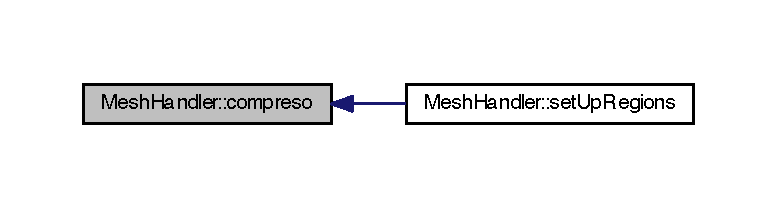
\includegraphics[width=350pt]{classMeshHandler_a3c8a354d214222155cb4eecf8214c938_icgraph}
\end{center}
\end{figure}


\hypertarget{classMeshHandler_a9d273c3ff67bed747b4a35bf24d96b41}{\index{Mesh\-Handler@{Mesh\-Handler}!compute\-Mesh\-Measures@{compute\-Mesh\-Measures}}
\index{compute\-Mesh\-Measures@{compute\-Mesh\-Measures}!MeshHandler@{Mesh\-Handler}}
\subsubsection[{compute\-Mesh\-Measures}]{\setlength{\rightskip}{0pt plus 5cm}void Mesh\-Handler\-::compute\-Mesh\-Measures (
\begin{DoxyParamCaption}
{}
\end{DoxyParamCaption}
)}}\label{classMeshHandler_a9d273c3ff67bed747b4a35bf24d96b41}


funzione che calcola l'inverso del passo della mesh, h$^\wedge$-\/1 


\begin{DoxyCode}
343 \{
344     \textcolor{comment}{// Allocate the vector for the circumcenters}
345     gmm::resize(M\_circumcentersAbscissa, M\_meshFEMCoefficients.nb\_dof());
346     gmm::clear(M\_circumcentersAbscissa);
347 
348     gmm::resize(M\_circumcentersOrdinate, M\_meshFEMCoefficients.nb\_dof());
349     gmm::clear(M\_circumcentersOrdinate);
350 
351     \textcolor{comment}{// Allocate the vector for the edge midpoint}
352     gmm::resize(M\_edgeMidpointAbscissa, M\_meshFEMVector.nb\_dof());
353     gmm::clear(M\_edgeMidpointAbscissa);
354 
355     gmm::resize(M\_edgeMidpointOrdinate, M\_meshFEMVector.nb\_dof());
356     gmm::clear(M\_edgeMidpointOrdinate);
357 
358     \textcolor{comment}{// Allocate the vector for the edge length}
359     gmm::resize(M\_edgeLength, M\_meshFEMVector.nb\_dof());
360     gmm::clear(M\_edgeLength);
361     
362     
363     \textcolor{comment}{// Computes all the circumcenters}
364     \textcolor{keywordflow}{for} ( size\_type j=0; j< (M\_mesh.convex\_index()).size(); j++)
365     \{   
366         \textcolor{comment}{// Get the coordinates of the vertices of the current triangle}
367         bgeot::basic\_mesh::ref\_mesh\_pt\_ct coordinates = M\_mesh.points\_of\_convex(j);
368 
369         \textcolor{keywordflow}{for} ( size\_type \hyperlink{matrici_8m_a6f6ccfcf58b31cb6412107d9d5281426}{i} = 0; \hyperlink{matrici_8m_a6f6ccfcf58b31cb6412107d9d5281426}{i} < M\_mesh.nb\_faces\_of\_convex(j); ++\hyperlink{matrici_8m_a6f6ccfcf58b31cb6412107d9d5281426}{i} )
370         \{
371             
372             size\_type dof = M\_meshFEMVector.ind\_basic\_dof\_of\_element(j) [ \hyperlink{matrici_8m_a6f6ccfcf58b31cb6412107d9d5281426}{i} ];
373 
374             M\_edgeMidpointAbscissa [ dof ] = 0.5 * (coordinates [ \hyperlink{matrici_8m_a6f6ccfcf58b31cb6412107d9d5281426}{i} ] [ 0 ] + coordinates [ (
      \hyperlink{matrici_8m_a6f6ccfcf58b31cb6412107d9d5281426}{i} + 1) % 3 ] [ 0 ]);
375 
376             M\_edgeMidpointOrdinate [ dof ] = 0.5 * (coordinates [ \hyperlink{matrici_8m_a6f6ccfcf58b31cb6412107d9d5281426}{i} ] [ 1 ] + coordinates [ (
      \hyperlink{matrici_8m_a6f6ccfcf58b31cb6412107d9d5281426}{i} + 1) % 3 ] [ 1 ]);
377             
378             \textcolor{comment}{// Computes the edge length}
379             M\_edgeLength [ dof ] = \hyperlink{UsefulFunctions_8h_ad9cf8f3fe42287349e8e1b2f1f824958}{pointDistance}(coordinates [ \hyperlink{matrici_8m_a6f6ccfcf58b31cb6412107d9d5281426}{i} ] [ 0 ],
380                                     coordinates [ (i + 1) % 3 ] [ 0 ], coordinates [ i ] [ 1 ],
381                                     coordinates [ (i + 1) % 3 ] [ 1 ]);
382         \}
383 
384         \textcolor{comment}{// Computes the circumcenter}
385         \textcolor{keywordflow}{for} ( size\_type i = 0; i < M\_mesh.nb\_faces\_of\_convex(j); ++\hyperlink{matrici_8m_a6f6ccfcf58b31cb6412107d9d5281426}{i} )
386         \{
387             size\_type dof = M\_meshFEMVector.ind\_basic\_dof\_of\_element(j) [ \hyperlink{matrici_8m_a6f6ccfcf58b31cb6412107d9d5281426}{i} ];
388             
389             M\_circumcentersAbscissa [ j ] += 0.3 * M\_edgeMidpointAbscissa [ dof ];
390             
391             M\_circumcentersOrdinate [ j ] += 0.3 * M\_edgeMidpointOrdinate [ dof ];
392         \}
393     
394     \}
395     
396     gmm::resize(M\_circumcentersDistance, M\_meshFEMVector.nb\_dof());
397     gmm::clear(M\_circumcentersDistance);
398 
399     \textcolor{comment}{// Computes all the distances between the circumcenters of adjacent triangels}
400     \textcolor{keywordflow}{for} ( size\_type j=0; j< (M\_mesh.convex\_index()).size(); j++)
401     \{
402         \textcolor{keywordflow}{for} ( size\_type i = 0; i < M\_mesh.nb\_faces\_of\_convex(j); ++\hyperlink{matrici_8m_a6f6ccfcf58b31cb6412107d9d5281426}{i} )
403         \{
404             \textcolor{comment}{// For each face get the corresponding neighbour}
405             size\_type neighbour = M\_mesh.neighbour\_of\_convex(j, i);
406 
407             size\_type dof = M\_meshFEMVector.ind\_basic\_dof\_of\_element(j) [ \hyperlink{matrici_8m_a6f6ccfcf58b31cb6412107d9d5281426}{i} ];
408  
409             \textcolor{comment}{// Check if the neighbour exist, i.e. not a boundary element}
410             \textcolor{keywordflow}{if} ( neighbour != size\_type(-1) )
411             \{
412 
413                 \textcolor{comment}{// Check if the position in M\_circumcentersDistance is jet filled}
414                 \textcolor{keywordflow}{if} ( M\_circumcentersDistance [ dof ] == 0 )
415                 \{
416                     \textcolor{comment}{// Computes the distance of the circumcenters}
417                     M\_circumcentersDistance [ dof ] = \hyperlink{UsefulFunctions_8h_ad9cf8f3fe42287349e8e1b2f1f824958}{pointDistance}( M\_circumcentersAbscissa [
       neighbour ],
418                                                                      M\_circumcentersAbscissa [ j ],
419                                                                      M\_circumcentersOrdinate [ neighbour ],
420                                                                      M\_circumcentersOrdinate [ j ]);
421 
422                 \}
423             \}
424             \textcolor{keywordflow}{else}
425             \{
426                 \textcolor{comment}{// Boundary face, the position is not jet filled}
427                 M\_circumcentersDistance [ dof ] = \hyperlink{UsefulFunctions_8h_ad9cf8f3fe42287349e8e1b2f1f824958}{pointDistance}( M\_edgeMidpointAbscissa [ dof 
      ],
428                                                                  M\_circumcentersAbscissa [ j ],
429                                                                  M\_edgeMidpointOrdinate [ dof ],
430                                                                  M\_circumcentersOrdinate [ j ]);
431             \}
432         \}
433     \}
434 
435     \textcolor{comment}{// Computing h^(-1) on external boudaries.}
436     \textcolor{comment}{// Useful for impose the boundary condition with Nitsche penalisation}
437 
438     \textcolor{comment}{// Allocate the vector for the M\_mediumMesh size}
439     gmm::resize(M\_meshSize, M\_meshFEMScalar.nb\_dof());
440     gmm::clear(M\_meshSize);
441 
442     \textcolor{comment}{// Allocate the vector for the inverse of the M\_mediumMesh size}
443     gmm::resize(M\_inverseMeshSize, M\_meshFEMScalar.nb\_dof());
444     gmm::clear(M\_inverseMeshSize);
445 
446     \textcolor{keywordflow}{for} ( size\_type j=0; j< (M\_mesh.convex\_index()).size(); j++)
447     \{
448         \textcolor{comment}{// Select the current dof}
449         size\_type dofScalar = M\_meshFEMScalar.ind\_basic\_dof\_of\_element(j) [ 0 ];
450 
451         \hyperlink{Core_8h_a4e75b5863535ba1dd79942de2846eff0}{scalarVector\_Type} edges(3, 0.);
452 
453         \textcolor{keywordflow}{for} ( size\_type i = 0; i < M\_mesh.nb\_faces\_of\_convex(j); ++\hyperlink{matrici_8m_a6f6ccfcf58b31cb6412107d9d5281426}{i} )
454         \{
455 
456             size\_type dofVector = M\_meshFEMVector.ind\_basic\_dof\_of\_element( j ) [ 
      \hyperlink{matrici_8m_a6f6ccfcf58b31cb6412107d9d5281426}{i} ];
457 
458             \textcolor{comment}{// Computes the edge length}
459             edges [ \hyperlink{matrici_8m_a6f6ccfcf58b31cb6412107d9d5281426}{i} ] = M\_edgeLength [ dofVector ];
460 
461         \}
462 
463         \textcolor{comment}{// Estimate the element size}
464         M\_meshSize [ dofScalar ] = *(std::max\_element ( edges.begin(), edges.end() ));
465 
466         \textcolor{comment}{// Compute h^(-1)}
467         M\_inverseMeshSize [ dofScalar ] = 1.0 / M\_meshSize [ dofScalar ];
468     \}
469 
470     \textcolor{keywordflow}{return};
471     
472 \}\textcolor{comment}{// computeMeshMeasures}
\end{DoxyCode}


Questo è il grafo delle chiamate per questa funzione\-:\nopagebreak
\begin{figure}[H]
\begin{center}
\leavevmode
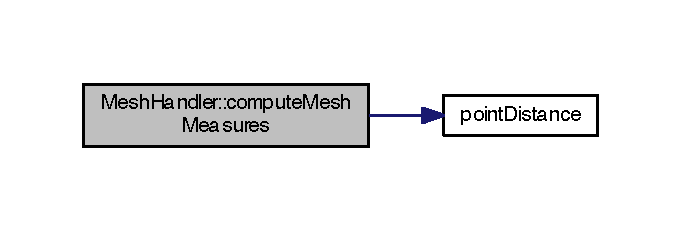
\includegraphics[width=327pt]{classMeshHandler_a9d273c3ff67bed747b4a35bf24d96b41_cgraph}
\end{center}
\end{figure}


\hypertarget{classMeshHandler_a616fa00edafb858d897fb64d80c69c15}{\index{Mesh\-Handler@{Mesh\-Handler}!get\-Circumcenters\-Distance@{get\-Circumcenters\-Distance}}
\index{get\-Circumcenters\-Distance@{get\-Circumcenters\-Distance}!MeshHandler@{Mesh\-Handler}}
\subsubsection[{get\-Circumcenters\-Distance}]{\setlength{\rightskip}{0pt plus 5cm}const scalar\-\_\-type\& Mesh\-Handler\-::get\-Circumcenters\-Distance (
\begin{DoxyParamCaption}
\item[{const size\-\_\-type \&}]{dof}
\end{DoxyParamCaption}
) const\hspace{0.3cm}{\ttfamily [inline]}}}\label{classMeshHandler_a616fa00edafb858d897fb64d80c69c15}

\begin{DoxyCode}
339     \{
340         \textcolor{keywordflow}{return} M\_circumcentersDistance [ dof ];
341     \}
\end{DoxyCode}
\hypertarget{classMeshHandler_a15243aa9754c8b96f35f49d16cee4c1e}{\index{Mesh\-Handler@{Mesh\-Handler}!get\-Count\-Extended\-D\-O\-F\-Scalar@{get\-Count\-Extended\-D\-O\-F\-Scalar}}
\index{get\-Count\-Extended\-D\-O\-F\-Scalar@{get\-Count\-Extended\-D\-O\-F\-Scalar}!MeshHandler@{Mesh\-Handler}}
\subsubsection[{get\-Count\-Extended\-D\-O\-F\-Scalar}]{\setlength{\rightskip}{0pt plus 5cm}size\-\_\-type Mesh\-Handler\-::get\-Count\-Extended\-D\-O\-F\-Scalar (
\begin{DoxyParamCaption}
\item[{const scalar\-\_\-type \&}]{id}
\end{DoxyParamCaption}
) const}}\label{classMeshHandler_a15243aa9754c8b96f35f49d16cee4c1e}


funzione che conta il numero di gradi di libertà estesi per la pressione per tutte le fratture che hanno indice $<$ id 


\begin{DoxyParams}{Parametri}
{\em id,\-:} & indice che identifica una frattura \\
\hline
\end{DoxyParams}
\begin{DoxyReturn}{Restituisce}
numero dei gradi di libertà 
\end{DoxyReturn}

\begin{DoxyCode}
539 \{
540     size\_type total = 0;
541 
542     \textcolor{keywordflow}{if} ( \textcolor{keywordtype}{id} < 0 )
543     \{
544         \textcolor{keywordflow}{return} total;
545     \}
546 
547     \textcolor{keywordflow}{for} ( size\_type f = 0; f <= id; ++f )
548     \{
549         total += M\_extendedDOFScalar [ f ].size();
550     \}
551 
552     \textcolor{keywordflow}{return} total;
553 \}\textcolor{comment}{// getCountExtendedDOFScalar}
\end{DoxyCode}
\hypertarget{classMeshHandler_a31feb5b56638ea15982435239f196d7d}{\index{Mesh\-Handler@{Mesh\-Handler}!get\-Count\-Extended\-D\-O\-F\-Vector@{get\-Count\-Extended\-D\-O\-F\-Vector}}
\index{get\-Count\-Extended\-D\-O\-F\-Vector@{get\-Count\-Extended\-D\-O\-F\-Vector}!MeshHandler@{Mesh\-Handler}}
\subsubsection[{get\-Count\-Extended\-D\-O\-F\-Vector}]{\setlength{\rightskip}{0pt plus 5cm}size\-\_\-type Mesh\-Handler\-::get\-Count\-Extended\-D\-O\-F\-Vector (
\begin{DoxyParamCaption}
\item[{const scalar\-\_\-type \&}]{id}
\end{DoxyParamCaption}
) const}}\label{classMeshHandler_a31feb5b56638ea15982435239f196d7d}


funzione che conta il numero di gradi di libertà estesi per la velocità per tutte le fratture che hanno indice $<$ id 


\begin{DoxyCode}
557 \{
558     size\_type total = 0;
559 
560     \textcolor{keywordflow}{if} ( \textcolor{keywordtype}{id} < 0 )
561     \{
562         \textcolor{keywordflow}{return} total;
563     \}
564 
565     \textcolor{keywordflow}{for} ( size\_type f = 0; f <= id; ++f )
566     \{
567         total += M\_extendedDOFVector [ f ].size();
568     \}
569 
570     \textcolor{keywordflow}{return} total;
571 \}\textcolor{comment}{// getCountExtendedDOFVector}
\end{DoxyCode}
\hypertarget{classMeshHandler_acdc0169a2f27d56c390c83c913cc2004}{\index{Mesh\-Handler@{Mesh\-Handler}!get\-Count\-Extended\-Intersect\-D\-O\-F\-Scalar@{get\-Count\-Extended\-Intersect\-D\-O\-F\-Scalar}}
\index{get\-Count\-Extended\-Intersect\-D\-O\-F\-Scalar@{get\-Count\-Extended\-Intersect\-D\-O\-F\-Scalar}!MeshHandler@{Mesh\-Handler}}
\subsubsection[{get\-Count\-Extended\-Intersect\-D\-O\-F\-Scalar}]{\setlength{\rightskip}{0pt plus 5cm}size\-\_\-type Mesh\-Handler\-::get\-Count\-Extended\-Intersect\-D\-O\-F\-Scalar (
\begin{DoxyParamCaption}
{}
\end{DoxyParamCaption}
) const\hspace{0.3cm}{\ttfamily [inline]}}}\label{classMeshHandler_acdc0169a2f27d56c390c83c913cc2004}

\begin{DoxyCode}
297     \{
298         \textcolor{keywordflow}{return} M\_extendedIntersectDOFScalar.size();
299     \}
\end{DoxyCode}
\hypertarget{classMeshHandler_a703d9e9f870b3802d8159aa0da398216}{\index{Mesh\-Handler@{Mesh\-Handler}!get\-Count\-Extended\-Intersect\-D\-O\-F\-Vector@{get\-Count\-Extended\-Intersect\-D\-O\-F\-Vector}}
\index{get\-Count\-Extended\-Intersect\-D\-O\-F\-Vector@{get\-Count\-Extended\-Intersect\-D\-O\-F\-Vector}!MeshHandler@{Mesh\-Handler}}
\subsubsection[{get\-Count\-Extended\-Intersect\-D\-O\-F\-Vector}]{\setlength{\rightskip}{0pt plus 5cm}size\-\_\-type Mesh\-Handler\-::get\-Count\-Extended\-Intersect\-D\-O\-F\-Vector (
\begin{DoxyParamCaption}
{}
\end{DoxyParamCaption}
) const\hspace{0.3cm}{\ttfamily [inline]}}}\label{classMeshHandler_a703d9e9f870b3802d8159aa0da398216}

\begin{DoxyCode}
309     \{
310         \textcolor{keywordflow}{return} M\_extendedIntersectDOFVector.size();
311     \}
\end{DoxyCode}
\hypertarget{classMeshHandler_a32b8f88e589acf24d4430959b9f99b79}{\index{Mesh\-Handler@{Mesh\-Handler}!get\-Edge\-Length@{get\-Edge\-Length}}
\index{get\-Edge\-Length@{get\-Edge\-Length}!MeshHandler@{Mesh\-Handler}}
\subsubsection[{get\-Edge\-Length}]{\setlength{\rightskip}{0pt plus 5cm}const scalar\-\_\-type\& Mesh\-Handler\-::get\-Edge\-Length (
\begin{DoxyParamCaption}
\item[{const size\-\_\-type \&}]{dof}
\end{DoxyParamCaption}
) const\hspace{0.3cm}{\ttfamily [inline]}}}\label{classMeshHandler_a32b8f88e589acf24d4430959b9f99b79}

\begin{DoxyCode}
333     \{
334         \textcolor{keywordflow}{return} M\_edgeLength [ dof ];
335     \}
\end{DoxyCode}
\hypertarget{classMeshHandler_a293bf3ce9492a84f4b510327bdb11939}{\index{Mesh\-Handler@{Mesh\-Handler}!get\-Extended\-D\-O\-F\-Scalar@{get\-Extended\-D\-O\-F\-Scalar}}
\index{get\-Extended\-D\-O\-F\-Scalar@{get\-Extended\-D\-O\-F\-Scalar}!MeshHandler@{Mesh\-Handler}}
\subsubsection[{get\-Extended\-D\-O\-F\-Scalar}]{\setlength{\rightskip}{0pt plus 5cm}const {\bf size\-Vector\-\_\-\-Type}\& Mesh\-Handler\-::get\-Extended\-D\-O\-F\-Scalar (
\begin{DoxyParamCaption}
\item[{const size\-\_\-type \&}]{id}
\end{DoxyParamCaption}
) const\hspace{0.3cm}{\ttfamily [inline]}}}\label{classMeshHandler_a293bf3ce9492a84f4b510327bdb11939}

\begin{DoxyCode}
257     \{
258         \textcolor{keywordflow}{return} M\_extendedDOFScalar [ id ];
259     \}
\end{DoxyCode}
\hypertarget{classMeshHandler_a6011a3ef304f58d262c1f94a60a7146d}{\index{Mesh\-Handler@{Mesh\-Handler}!get\-Extended\-D\-O\-F\-Scalar@{get\-Extended\-D\-O\-F\-Scalar}}
\index{get\-Extended\-D\-O\-F\-Scalar@{get\-Extended\-D\-O\-F\-Scalar}!MeshHandler@{Mesh\-Handler}}
\subsubsection[{get\-Extended\-D\-O\-F\-Scalar}]{\setlength{\rightskip}{0pt plus 5cm}const size\-\_\-type\& Mesh\-Handler\-::get\-Extended\-D\-O\-F\-Scalar (
\begin{DoxyParamCaption}
\item[{const size\-\_\-type \&}]{id, }
\item[{const size\-\_\-type \&}]{dof}
\end{DoxyParamCaption}
) const\hspace{0.3cm}{\ttfamily [inline]}}}\label{classMeshHandler_a6011a3ef304f58d262c1f94a60a7146d}

\begin{DoxyCode}
278     \{
279         \textcolor{keywordflow}{return} M\_extendedDOFScalar [ id ] [ dof ];
280     \}
\end{DoxyCode}
\hypertarget{classMeshHandler_af0e395f252eaa17da529279389a8b70a}{\index{Mesh\-Handler@{Mesh\-Handler}!get\-Extended\-D\-O\-F\-Vector@{get\-Extended\-D\-O\-F\-Vector}}
\index{get\-Extended\-D\-O\-F\-Vector@{get\-Extended\-D\-O\-F\-Vector}!MeshHandler@{Mesh\-Handler}}
\subsubsection[{get\-Extended\-D\-O\-F\-Vector}]{\setlength{\rightskip}{0pt plus 5cm}const {\bf size\-Vector\-\_\-\-Type}\& Mesh\-Handler\-::get\-Extended\-D\-O\-F\-Vector (
\begin{DoxyParamCaption}
\item[{const size\-\_\-type \&}]{id}
\end{DoxyParamCaption}
) const\hspace{0.3cm}{\ttfamily [inline]}}}\label{classMeshHandler_af0e395f252eaa17da529279389a8b70a}

\begin{DoxyCode}
284     \{
285         \textcolor{keywordflow}{return} M\_extendedDOFVector [ id ];
286     \}
\end{DoxyCode}
\hypertarget{classMeshHandler_a758ccd3a35b85628d241dc528e773446}{\index{Mesh\-Handler@{Mesh\-Handler}!get\-Extended\-D\-O\-F\-Vector@{get\-Extended\-D\-O\-F\-Vector}}
\index{get\-Extended\-D\-O\-F\-Vector@{get\-Extended\-D\-O\-F\-Vector}!MeshHandler@{Mesh\-Handler}}
\subsubsection[{get\-Extended\-D\-O\-F\-Vector}]{\setlength{\rightskip}{0pt plus 5cm}const size\-\_\-type\& Mesh\-Handler\-::get\-Extended\-D\-O\-F\-Vector (
\begin{DoxyParamCaption}
\item[{const size\-\_\-type \&}]{id, }
\item[{const size\-\_\-type \&}]{dof}
\end{DoxyParamCaption}
) const\hspace{0.3cm}{\ttfamily [inline]}}}\label{classMeshHandler_a758ccd3a35b85628d241dc528e773446}

\begin{DoxyCode}
291     \{
292         \textcolor{keywordflow}{return} M\_extendedDOFVector [ id ] [ dof ];
293     \}
\end{DoxyCode}
\hypertarget{classMeshHandler_a6b64278aa62abcf620d3583d7c006036}{\index{Mesh\-Handler@{Mesh\-Handler}!get\-Extended\-Intersect\-D\-O\-F\-Scalar@{get\-Extended\-Intersect\-D\-O\-F\-Scalar}}
\index{get\-Extended\-Intersect\-D\-O\-F\-Scalar@{get\-Extended\-Intersect\-D\-O\-F\-Scalar}!MeshHandler@{Mesh\-Handler}}
\subsubsection[{get\-Extended\-Intersect\-D\-O\-F\-Scalar}]{\setlength{\rightskip}{0pt plus 5cm}const {\bf size\-Vector\-\_\-\-Type}\& Mesh\-Handler\-::get\-Extended\-Intersect\-D\-O\-F\-Scalar (
\begin{DoxyParamCaption}
{}
\end{DoxyParamCaption}
) const\hspace{0.3cm}{\ttfamily [inline]}}}\label{classMeshHandler_a6b64278aa62abcf620d3583d7c006036}

\begin{DoxyCode}
303     \{
304         \textcolor{keywordflow}{return} M\_extendedIntersectDOFScalar;
305     \}
\end{DoxyCode}
\hypertarget{classMeshHandler_a32a3e4114f8f64d8d49c8d8d579a5e13}{\index{Mesh\-Handler@{Mesh\-Handler}!get\-Extended\-Intersect\-D\-O\-F\-Vector@{get\-Extended\-Intersect\-D\-O\-F\-Vector}}
\index{get\-Extended\-Intersect\-D\-O\-F\-Vector@{get\-Extended\-Intersect\-D\-O\-F\-Vector}!MeshHandler@{Mesh\-Handler}}
\subsubsection[{get\-Extended\-Intersect\-D\-O\-F\-Vector}]{\setlength{\rightskip}{0pt plus 5cm}const {\bf size\-Vector\-\_\-\-Type}\& Mesh\-Handler\-::get\-Extended\-Intersect\-D\-O\-F\-Vector (
\begin{DoxyParamCaption}
{}
\end{DoxyParamCaption}
) const\hspace{0.3cm}{\ttfamily [inline]}}}\label{classMeshHandler_a32a3e4114f8f64d8d49c8d8d579a5e13}

\begin{DoxyCode}
315     \{
316         \textcolor{keywordflow}{return} M\_extendedIntersectDOFVector;
317     \}
\end{DoxyCode}
\hypertarget{classMeshHandler_a007db33b8b43e68e059f1f989c0f79fa}{\index{Mesh\-Handler@{Mesh\-Handler}!get\-F\-E\-M\-Type\-Pressure@{get\-F\-E\-M\-Type\-Pressure}}
\index{get\-F\-E\-M\-Type\-Pressure@{get\-F\-E\-M\-Type\-Pressure}!MeshHandler@{Mesh\-Handler}}
\subsubsection[{get\-F\-E\-M\-Type\-Pressure}]{\setlength{\rightskip}{0pt plus 5cm}std\-::string Mesh\-Handler\-::get\-F\-E\-M\-Type\-Pressure (
\begin{DoxyParamCaption}
{}
\end{DoxyParamCaption}
) const\hspace{0.3cm}{\ttfamily [inline]}}}\label{classMeshHandler_a007db33b8b43e68e059f1f989c0f79fa}

\begin{DoxyCode}
191     \{
192         \textcolor{keywordflow}{return} M\_fEMTypeScalar;
193     \}
\end{DoxyCode}
\hypertarget{classMeshHandler_a79d87d2c1b1d01e942efe2678025c4a3}{\index{Mesh\-Handler@{Mesh\-Handler}!get\-F\-E\-M\-Type\-Velocity@{get\-F\-E\-M\-Type\-Velocity}}
\index{get\-F\-E\-M\-Type\-Velocity@{get\-F\-E\-M\-Type\-Velocity}!MeshHandler@{Mesh\-Handler}}
\subsubsection[{get\-F\-E\-M\-Type\-Velocity}]{\setlength{\rightskip}{0pt plus 5cm}std\-::string Mesh\-Handler\-::get\-F\-E\-M\-Type\-Velocity (
\begin{DoxyParamCaption}
{}
\end{DoxyParamCaption}
) const\hspace{0.3cm}{\ttfamily [inline]}}}\label{classMeshHandler_a79d87d2c1b1d01e942efe2678025c4a3}

\begin{DoxyCode}
185     \{
186         \textcolor{keywordflow}{return} M\_fEMTypeVector;
187     \}
\end{DoxyCode}
\hypertarget{classMeshHandler_a57750679882b57b28f65b6e31c3a6aa8}{\index{Mesh\-Handler@{Mesh\-Handler}!get\-Geometric\-Transformation@{get\-Geometric\-Transformation}}
\index{get\-Geometric\-Transformation@{get\-Geometric\-Transformation}!MeshHandler@{Mesh\-Handler}}
\subsubsection[{get\-Geometric\-Transformation}]{\setlength{\rightskip}{0pt plus 5cm}const bgeot\-::pgeometric\-\_\-trans\& Mesh\-Handler\-::get\-Geometric\-Transformation (
\begin{DoxyParamCaption}
{}
\end{DoxyParamCaption}
) const\hspace{0.3cm}{\ttfamily [inline]}}}\label{classMeshHandler_a57750679882b57b28f65b6e31c3a6aa8}

\begin{DoxyCode}
321     \{
322         \textcolor{keywordflow}{return} M\_geometricTransformation;
323     \}
\end{DoxyCode}
\hypertarget{classMeshHandler_a664d02d7ec6352339c90457c8106b92e}{\index{Mesh\-Handler@{Mesh\-Handler}!get\-Inclination@{get\-Inclination}}
\index{get\-Inclination@{get\-Inclination}!MeshHandler@{Mesh\-Handler}}
\subsubsection[{get\-Inclination}]{\setlength{\rightskip}{0pt plus 5cm}scalar\-\_\-type Mesh\-Handler\-::get\-Inclination (
\begin{DoxyParamCaption}
{}
\end{DoxyParamCaption}
) const\hspace{0.3cm}{\ttfamily [inline]}}}\label{classMeshHandler_a664d02d7ec6352339c90457c8106b92e}
\begin{DoxyReturn}{Restituisce}
M\-\_\-inclination\-: grandezza che indica di quanto il dominio reale è inclinato rispetto al dominio di riferimento 
\end{DoxyReturn}

\begin{DoxyCode}
106     \{
107         \textcolor{keywordflow}{return} M\_inclination;
108     \}
\end{DoxyCode}
\hypertarget{classMeshHandler_a0a25e658aff6ff2f1c06f04b847b792d}{\index{Mesh\-Handler@{Mesh\-Handler}!get\-Integration\-Method\-Scalar@{get\-Integration\-Method\-Scalar}}
\index{get\-Integration\-Method\-Scalar@{get\-Integration\-Method\-Scalar}!MeshHandler@{Mesh\-Handler}}
\subsubsection[{get\-Integration\-Method\-Scalar}]{\setlength{\rightskip}{0pt plus 5cm}const getfem\-::mesh\-\_\-im\& Mesh\-Handler\-::get\-Integration\-Method\-Scalar (
\begin{DoxyParamCaption}
{}
\end{DoxyParamCaption}
) const\hspace{0.3cm}{\ttfamily [inline]}}}\label{classMeshHandler_a0a25e658aff6ff2f1c06f04b847b792d}

\begin{DoxyCode}
221     \{
222         \textcolor{keywordflow}{return} M\_integrationMethodScalar;
223     \}
\end{DoxyCode}
\hypertarget{classMeshHandler_afd0fbe553d40c2f0dd42e36410bae3a7}{\index{Mesh\-Handler@{Mesh\-Handler}!get\-Integration\-Method\-Vector@{get\-Integration\-Method\-Vector}}
\index{get\-Integration\-Method\-Vector@{get\-Integration\-Method\-Vector}!MeshHandler@{Mesh\-Handler}}
\subsubsection[{get\-Integration\-Method\-Vector}]{\setlength{\rightskip}{0pt plus 5cm}const getfem\-::mesh\-\_\-im\& Mesh\-Handler\-::get\-Integration\-Method\-Vector (
\begin{DoxyParamCaption}
{}
\end{DoxyParamCaption}
) const\hspace{0.3cm}{\ttfamily [inline]}}}\label{classMeshHandler_afd0fbe553d40c2f0dd42e36410bae3a7}

\begin{DoxyCode}
215     \{
216         \textcolor{keywordflow}{return} M\_integrationMethodVector;
217     \}
\end{DoxyCode}
\hypertarget{classMeshHandler_a7e8638201a709e36dafa14998b2ba763}{\index{Mesh\-Handler@{Mesh\-Handler}!get\-Integration\-Type\-Pressure@{get\-Integration\-Type\-Pressure}}
\index{get\-Integration\-Type\-Pressure@{get\-Integration\-Type\-Pressure}!MeshHandler@{Mesh\-Handler}}
\subsubsection[{get\-Integration\-Type\-Pressure}]{\setlength{\rightskip}{0pt plus 5cm}std\-::string Mesh\-Handler\-::get\-Integration\-Type\-Pressure (
\begin{DoxyParamCaption}
{}
\end{DoxyParamCaption}
) const\hspace{0.3cm}{\ttfamily [inline]}}}\label{classMeshHandler_a7e8638201a709e36dafa14998b2ba763}

\begin{DoxyCode}
179     \{
180         \textcolor{keywordflow}{return} M\_integrationTypeScalar;
181     \}
\end{DoxyCode}
\hypertarget{classMeshHandler_ac9def34ac3cf1939389a6af08fd92111}{\index{Mesh\-Handler@{Mesh\-Handler}!get\-Integration\-Type\-Velocity@{get\-Integration\-Type\-Velocity}}
\index{get\-Integration\-Type\-Velocity@{get\-Integration\-Type\-Velocity}!MeshHandler@{Mesh\-Handler}}
\subsubsection[{get\-Integration\-Type\-Velocity}]{\setlength{\rightskip}{0pt plus 5cm}std\-::string Mesh\-Handler\-::get\-Integration\-Type\-Velocity (
\begin{DoxyParamCaption}
{}
\end{DoxyParamCaption}
) const\hspace{0.3cm}{\ttfamily [inline]}}}\label{classMeshHandler_ac9def34ac3cf1939389a6af08fd92111}

\begin{DoxyCode}
173     \{
174         \textcolor{keywordflow}{return} M\_integrationTypeVector;
175     \}
\end{DoxyCode}
\hypertarget{classMeshHandler_a05fa48c67a3fde6594fa3721785b9ce6}{\index{Mesh\-Handler@{Mesh\-Handler}!get\-Inverse\-Mesh\-Size@{get\-Inverse\-Mesh\-Size}}
\index{get\-Inverse\-Mesh\-Size@{get\-Inverse\-Mesh\-Size}!MeshHandler@{Mesh\-Handler}}
\subsubsection[{get\-Inverse\-Mesh\-Size}]{\setlength{\rightskip}{0pt plus 5cm}const {\bf scalar\-Vector\-\_\-\-Type}\& Mesh\-Handler\-::get\-Inverse\-Mesh\-Size (
\begin{DoxyParamCaption}
{}
\end{DoxyParamCaption}
) const\hspace{0.3cm}{\ttfamily [inline]}}}\label{classMeshHandler_a05fa48c67a3fde6594fa3721785b9ce6}

\begin{DoxyCode}
245     \{
246         \textcolor{keywordflow}{return} M\_inverseMeshSize;
247     \}
\end{DoxyCode}
\hypertarget{classMeshHandler_a36f6694bfd1a75bfb0a2a7c6ec69500f}{\index{Mesh\-Handler@{Mesh\-Handler}!get\-Inverse\-Mesh\-Size\-D\-O\-F@{get\-Inverse\-Mesh\-Size\-D\-O\-F}}
\index{get\-Inverse\-Mesh\-Size\-D\-O\-F@{get\-Inverse\-Mesh\-Size\-D\-O\-F}!MeshHandler@{Mesh\-Handler}}
\subsubsection[{get\-Inverse\-Mesh\-Size\-D\-O\-F}]{\setlength{\rightskip}{0pt plus 5cm}const scalar\-\_\-type\& Mesh\-Handler\-::get\-Inverse\-Mesh\-Size\-D\-O\-F (
\begin{DoxyParamCaption}
\item[{const size\-\_\-type \&}]{dof}
\end{DoxyParamCaption}
) const\hspace{0.3cm}{\ttfamily [inline]}}}\label{classMeshHandler_a36f6694bfd1a75bfb0a2a7c6ec69500f}

\begin{DoxyCode}
251     \{
252         \textcolor{keywordflow}{return} M\_inverseMeshSize [ dof ];
253     \}
\end{DoxyCode}
\hypertarget{classMeshHandler_a7eae9c85043ed3a26605dce2b1f3d6d2}{\index{Mesh\-Handler@{Mesh\-Handler}!get\-Length\-Abscissa@{get\-Length\-Abscissa}}
\index{get\-Length\-Abscissa@{get\-Length\-Abscissa}!MeshHandler@{Mesh\-Handler}}
\subsubsection[{get\-Length\-Abscissa}]{\setlength{\rightskip}{0pt plus 5cm}scalar\-\_\-type Mesh\-Handler\-::get\-Length\-Abscissa (
\begin{DoxyParamCaption}
{}
\end{DoxyParamCaption}
) const\hspace{0.3cm}{\ttfamily [inline]}}}\label{classMeshHandler_a7eae9c85043ed3a26605dce2b1f3d6d2}
\begin{DoxyReturn}{Restituisce}
M\-\_\-length\-Abscissa\-: grandezza che indica la lunghezza dell'ascissa del dominio reale 
\end{DoxyReturn}

\begin{DoxyCode}
115     \{
116         \textcolor{keywordflow}{return} M\_lengthAbscissa;
117     \}
\end{DoxyCode}
\hypertarget{classMeshHandler_a6935edc0af8e28979b2c294daa6e789e}{\index{Mesh\-Handler@{Mesh\-Handler}!get\-Length\-Ordinate@{get\-Length\-Ordinate}}
\index{get\-Length\-Ordinate@{get\-Length\-Ordinate}!MeshHandler@{Mesh\-Handler}}
\subsubsection[{get\-Length\-Ordinate}]{\setlength{\rightskip}{0pt plus 5cm}scalar\-\_\-type Mesh\-Handler\-::get\-Length\-Ordinate (
\begin{DoxyParamCaption}
{}
\end{DoxyParamCaption}
) const\hspace{0.3cm}{\ttfamily [inline]}}}\label{classMeshHandler_a6935edc0af8e28979b2c294daa6e789e}
\begin{DoxyReturn}{Restituisce}
M\-\_\-length\-Ordinate\-: grandezza che indica la lunghezza dell'ordinata del dominio reale 
\end{DoxyReturn}

\begin{DoxyCode}
124     \{
125         \textcolor{keywordflow}{return} M\_lengthOrdinate;
126     \}
\end{DoxyCode}
\hypertarget{classMeshHandler_a924c3c0d8020cc76bbc2773b634a3ed1}{\index{Mesh\-Handler@{Mesh\-Handler}!get\-Length\-Quota@{get\-Length\-Quota}}
\index{get\-Length\-Quota@{get\-Length\-Quota}!MeshHandler@{Mesh\-Handler}}
\subsubsection[{get\-Length\-Quota}]{\setlength{\rightskip}{0pt plus 5cm}scalar\-\_\-type Mesh\-Handler\-::get\-Length\-Quota (
\begin{DoxyParamCaption}
{}
\end{DoxyParamCaption}
) const\hspace{0.3cm}{\ttfamily [inline]}}}\label{classMeshHandler_a924c3c0d8020cc76bbc2773b634a3ed1}
\begin{DoxyReturn}{Restituisce}
M\-\_\-length\-Quota\-: grandezza che indica la lunghezza della quota del dominio reale 
\end{DoxyReturn}

\begin{DoxyCode}
133     \{
134         \textcolor{keywordflow}{return} M\_lengthQuota;
135     \}
\end{DoxyCode}
\hypertarget{classMeshHandler_ac2dba1bdf2c6c3f574de03f2cdd6f78d}{\index{Mesh\-Handler@{Mesh\-Handler}!get\-Mesh@{get\-Mesh}}
\index{get\-Mesh@{get\-Mesh}!MeshHandler@{Mesh\-Handler}}
\subsubsection[{get\-Mesh}]{\setlength{\rightskip}{0pt plus 5cm}const getfem\-::mesh\& Mesh\-Handler\-::get\-Mesh (
\begin{DoxyParamCaption}
{}
\end{DoxyParamCaption}
) const\hspace{0.3cm}{\ttfamily [inline]}}}\label{classMeshHandler_ac2dba1bdf2c6c3f574de03f2cdd6f78d}

\begin{DoxyCode}
149     \{
150         \textcolor{keywordflow}{return} M\_mesh;
151     \}
\end{DoxyCode}
\hypertarget{classMeshHandler_a8739e6e0ce82793e93a70b8a23bbc634}{\index{Mesh\-Handler@{Mesh\-Handler}!get\-Mesh@{get\-Mesh}}
\index{get\-Mesh@{get\-Mesh}!MeshHandler@{Mesh\-Handler}}
\subsubsection[{get\-Mesh}]{\setlength{\rightskip}{0pt plus 5cm}getfem\-::mesh\& Mesh\-Handler\-::get\-Mesh (
\begin{DoxyParamCaption}
{}
\end{DoxyParamCaption}
)\hspace{0.3cm}{\ttfamily [inline]}}}\label{classMeshHandler_a8739e6e0ce82793e93a70b8a23bbc634}

\begin{DoxyCode}
155     \{
156         \textcolor{keywordflow}{return} M\_mesh;
157     \}
\end{DoxyCode}
\hypertarget{classMeshHandler_a44953dabfaec9e6577f21c023f792b61}{\index{Mesh\-Handler@{Mesh\-Handler}!get\-Mesh\-F\-E\-M\-Coefficients@{get\-Mesh\-F\-E\-M\-Coefficients}}
\index{get\-Mesh\-F\-E\-M\-Coefficients@{get\-Mesh\-F\-E\-M\-Coefficients}!MeshHandler@{Mesh\-Handler}}
\subsubsection[{get\-Mesh\-F\-E\-M\-Coefficients}]{\setlength{\rightskip}{0pt plus 5cm}const getfem\-::mesh\-\_\-fem\& Mesh\-Handler\-::get\-Mesh\-F\-E\-M\-Coefficients (
\begin{DoxyParamCaption}
{}
\end{DoxyParamCaption}
) const\hspace{0.3cm}{\ttfamily [inline]}}}\label{classMeshHandler_a44953dabfaec9e6577f21c023f792b61}

\begin{DoxyCode}
197     \{
198         \textcolor{keywordflow}{return} M\_meshFEMCoefficients;
199     \}
\end{DoxyCode}
\hypertarget{classMeshHandler_aeedf6a1246d39207a92fc0a5ddbd439f}{\index{Mesh\-Handler@{Mesh\-Handler}!get\-Mesh\-F\-E\-M\-Scalar@{get\-Mesh\-F\-E\-M\-Scalar}}
\index{get\-Mesh\-F\-E\-M\-Scalar@{get\-Mesh\-F\-E\-M\-Scalar}!MeshHandler@{Mesh\-Handler}}
\subsubsection[{get\-Mesh\-F\-E\-M\-Scalar}]{\setlength{\rightskip}{0pt plus 5cm}const getfem\-::mesh\-\_\-fem\& Mesh\-Handler\-::get\-Mesh\-F\-E\-M\-Scalar (
\begin{DoxyParamCaption}
{}
\end{DoxyParamCaption}
) const\hspace{0.3cm}{\ttfamily [inline]}}}\label{classMeshHandler_aeedf6a1246d39207a92fc0a5ddbd439f}

\begin{DoxyCode}
203     \{
204         \textcolor{keywordflow}{return} M\_meshFEMScalar;
205     \}
\end{DoxyCode}
\hypertarget{classMeshHandler_a786a00ddf3a26b923a07b942ea2b2247}{\index{Mesh\-Handler@{Mesh\-Handler}!get\-Mesh\-F\-E\-M\-Vector@{get\-Mesh\-F\-E\-M\-Vector}}
\index{get\-Mesh\-F\-E\-M\-Vector@{get\-Mesh\-F\-E\-M\-Vector}!MeshHandler@{Mesh\-Handler}}
\subsubsection[{get\-Mesh\-F\-E\-M\-Vector}]{\setlength{\rightskip}{0pt plus 5cm}const getfem\-::mesh\-\_\-fem\& Mesh\-Handler\-::get\-Mesh\-F\-E\-M\-Vector (
\begin{DoxyParamCaption}
{}
\end{DoxyParamCaption}
) const\hspace{0.3cm}{\ttfamily [inline]}}}\label{classMeshHandler_a786a00ddf3a26b923a07b942ea2b2247}

\begin{DoxyCode}
209     \{
210         \textcolor{keywordflow}{return} M\_meshFEMVector;
211     \}
\end{DoxyCode}
\hypertarget{classMeshHandler_a8e4ede201bd0e5fa83ec7b7a42f2befa}{\index{Mesh\-Handler@{Mesh\-Handler}!get\-Mesh\-Level\-Set@{get\-Mesh\-Level\-Set}}
\index{get\-Mesh\-Level\-Set@{get\-Mesh\-Level\-Set}!MeshHandler@{Mesh\-Handler}}
\subsubsection[{get\-Mesh\-Level\-Set}]{\setlength{\rightskip}{0pt plus 5cm}getfem\-::mesh\-\_\-level\-\_\-set\& Mesh\-Handler\-::get\-Mesh\-Level\-Set (
\begin{DoxyParamCaption}
{}
\end{DoxyParamCaption}
)\hspace{0.3cm}{\ttfamily [inline]}}}\label{classMeshHandler_a8e4ede201bd0e5fa83ec7b7a42f2befa}

\begin{DoxyCode}
161     \{
162         \textcolor{keywordflow}{return} M\_meshLevelSet;
163     \}
\end{DoxyCode}
\hypertarget{classMeshHandler_ae176155967a168d4342ee9dfb72689e5}{\index{Mesh\-Handler@{Mesh\-Handler}!get\-Mesh\-Size@{get\-Mesh\-Size}}
\index{get\-Mesh\-Size@{get\-Mesh\-Size}!MeshHandler@{Mesh\-Handler}}
\subsubsection[{get\-Mesh\-Size}]{\setlength{\rightskip}{0pt plus 5cm}const {\bf scalar\-Vector\-\_\-\-Type}\& Mesh\-Handler\-::get\-Mesh\-Size (
\begin{DoxyParamCaption}
{}
\end{DoxyParamCaption}
) const\hspace{0.3cm}{\ttfamily [inline]}}}\label{classMeshHandler_ae176155967a168d4342ee9dfb72689e5}

\begin{DoxyCode}
239     \{
240         \textcolor{keywordflow}{return} M\_meshSize;
241     \}
\end{DoxyCode}
\hypertarget{classMeshHandler_aec42b571d6dec518833c5264e2e43830}{\index{Mesh\-Handler@{Mesh\-Handler}!get\-Mesh\-Type@{get\-Mesh\-Type}}
\index{get\-Mesh\-Type@{get\-Mesh\-Type}!MeshHandler@{Mesh\-Handler}}
\subsubsection[{get\-Mesh\-Type}]{\setlength{\rightskip}{0pt plus 5cm}std\-::string Mesh\-Handler\-::get\-Mesh\-Type (
\begin{DoxyParamCaption}
{}
\end{DoxyParamCaption}
) const\hspace{0.3cm}{\ttfamily [inline]}}}\label{classMeshHandler_aec42b571d6dec518833c5264e2e43830}
\begin{DoxyReturn}{Restituisce}
M\-\_\-mesh\-Type\-: std\-::string M\-\_\-mesh\-Type, grandezza che rappresenta una trasformazione per Get\-F\-E\-M++, definisce l'elemento di riferimento su cui è descritto il metodo di integrazione 
\end{DoxyReturn}

\begin{DoxyCode}
143     \{
144         \textcolor{keywordflow}{return} M\_meshType;
145     \}
\end{DoxyCode}
\hypertarget{classMeshHandler_a6b5defc6ac7c8c8c0c1b1c81c6a980e7}{\index{Mesh\-Handler@{Mesh\-Handler}!get\-Non\-Cut@{get\-Non\-Cut}}
\index{get\-Non\-Cut@{get\-Non\-Cut}!MeshHandler@{Mesh\-Handler}}
\subsubsection[{get\-Non\-Cut}]{\setlength{\rightskip}{0pt plus 5cm}{\bf size\-Vector\-\_\-\-Type}\& Mesh\-Handler\-::get\-Non\-Cut (
\begin{DoxyParamCaption}
{}
\end{DoxyParamCaption}
)\hspace{0.3cm}{\ttfamily [inline]}}}\label{classMeshHandler_a6b5defc6ac7c8c8c0c1b1c81c6a980e7}

\begin{DoxyCode}
327     \{
328         \textcolor{keywordflow}{return} M\_nonCut;
329     \}
\end{DoxyCode}
\hypertarget{classMeshHandler_adfb74826f08fd62a92200ebfe8ce3fbe}{\index{Mesh\-Handler@{Mesh\-Handler}!get\-Region@{get\-Region}}
\index{get\-Region@{get\-Region}!MeshHandler@{Mesh\-Handler}}
\subsubsection[{get\-Region}]{\setlength{\rightskip}{0pt plus 5cm}const getfem\-::mesh\-\_\-region\& Mesh\-Handler\-::get\-Region (
\begin{DoxyParamCaption}
\item[{const size\-\_\-type \&}]{region\-Flag}
\end{DoxyParamCaption}
) const\hspace{0.3cm}{\ttfamily [inline]}}}\label{classMeshHandler_adfb74826f08fd62a92200ebfe8ce3fbe}

\begin{DoxyCode}
227     \{
228         \textcolor{keywordflow}{return} M\_mesh.region(regionFlag);
229     \}
\end{DoxyCode}
\hypertarget{classMeshHandler_a36ba76b0940684abab86ef6e56fe1086}{\index{Mesh\-Handler@{Mesh\-Handler}!get\-Region@{get\-Region}}
\index{get\-Region@{get\-Region}!MeshHandler@{Mesh\-Handler}}
\subsubsection[{get\-Region}]{\setlength{\rightskip}{0pt plus 5cm}getfem\-::mesh\-\_\-region\& Mesh\-Handler\-::get\-Region (
\begin{DoxyParamCaption}
\item[{const size\-\_\-type \&}]{region\-Flag}
\end{DoxyParamCaption}
)\hspace{0.3cm}{\ttfamily [inline]}}}\label{classMeshHandler_a36ba76b0940684abab86ef6e56fe1086}

\begin{DoxyCode}
233     \{
234         \textcolor{keywordflow}{return} M\_mesh.region(regionFlag);
235     \}
\end{DoxyCode}
\hypertarget{classMeshHandler_a804b1168383f92f35f3c472f7ec58861}{\index{Mesh\-Handler@{Mesh\-Handler}!get\-Space\-Dimension@{get\-Space\-Dimension}}
\index{get\-Space\-Dimension@{get\-Space\-Dimension}!MeshHandler@{Mesh\-Handler}}
\subsubsection[{get\-Space\-Dimension}]{\setlength{\rightskip}{0pt plus 5cm}bgeot\-::dim\-\_\-type Mesh\-Handler\-::get\-Space\-Dimension (
\begin{DoxyParamCaption}
{}
\end{DoxyParamCaption}
) const\hspace{0.3cm}{\ttfamily [inline]}}}\label{classMeshHandler_a804b1168383f92f35f3c472f7ec58861}

\begin{DoxyCode}
167     \{
168         \textcolor{keywordflow}{return} M\_spaceDimension;
169     \}
\end{DoxyCode}
\hypertarget{classMeshHandler_af0c391bcac1ee103838b78d540b2b326}{\index{Mesh\-Handler@{Mesh\-Handler}!get\-Spatial\-Discretization@{get\-Spatial\-Discretization}}
\index{get\-Spatial\-Discretization@{get\-Spatial\-Discretization}!MeshHandler@{Mesh\-Handler}}
\subsubsection[{get\-Spatial\-Discretization}]{\setlength{\rightskip}{0pt plus 5cm}size\-\_\-type Mesh\-Handler\-::get\-Spatial\-Discretization (
\begin{DoxyParamCaption}
{}
\end{DoxyParamCaption}
) const\hspace{0.3cm}{\ttfamily [inline]}}}\label{classMeshHandler_af0c391bcac1ee103838b78d540b2b326}
\begin{DoxyReturn}{Restituisce}
M\-\_\-spatial\-Discretization\-: discretizzazione spaziale, numero di elementi in cui ogni lato del dominio viene suddiviso 
\end{DoxyReturn}

\begin{DoxyCode}
98     \{
99         \textcolor{keywordflow}{return} M\_spatialDiscretization;
100     \}
\end{DoxyCode}
\hypertarget{classMeshHandler_adf082b93f71c001f6f1252dd269ae8fa}{\index{Mesh\-Handler@{Mesh\-Handler}!print\-Cutted\-Elements@{print\-Cutted\-Elements}}
\index{print\-Cutted\-Elements@{print\-Cutted\-Elements}!MeshHandler@{Mesh\-Handler}}
\subsubsection[{print\-Cutted\-Elements}]{\setlength{\rightskip}{0pt plus 5cm}void Mesh\-Handler\-::print\-Cutted\-Elements (
\begin{DoxyParamCaption}
\item[{const std\-::string \&}]{vtk\-Folder = {\ttfamily \char`\"{}vtk/\char`\"{}}, }
\item[{const std\-::string \&}]{file\-Name = {\ttfamily \char`\"{}CuttedElements\char`\"{}}}
\end{DoxyParamCaption}
) const}}\label{classMeshHandler_adf082b93f71c001f6f1252dd269ae8fa}


funzione che esporta in formato .vtk per paraview gli elementi che sono tagliati dal level set M\-\_\-level\-Set pone pari a 1 se sono tagliati e 0 se non lo sono 


\begin{DoxyParams}{Parametri}
{\em vtk\-Folder,\-:} & nome della cartella in cui esportare \\
\hline
{\em file\-Name,\-:} & nome da dare al file da esportare con la soluzione \\
\hline
\end{DoxyParams}

\begin{DoxyCode}
516 \{
517     \textcolor{keyword}{const} size\_type numberFractures = M\_extendedDOFScalar.size();
518 
519     \hyperlink{Core_8h_a4e75b5863535ba1dd79942de2846eff0}{scalarVector\_Type} cuttedElements(M\_meshFEMScalar.nb\_dof(), 0);     \textcolor{comment}{// numero totale
       dei gradi di libertà}
520     
521     \textcolor{keywordflow}{for} ( size\_type f = 0; f < numberFractures; ++f )
522     \{
523         \textcolor{keyword}{const} \hyperlink{Core_8h_a83c51913d041a5001e8683434c09857f}{sizeVector\_Type}& extendedDOFScalar = M\_extendedDOFScalar [ f ];
524         \textcolor{keyword}{const} size\_type shiftExtended = extendedDOFScalar.size();
525 
526         \textcolor{keywordflow}{for} ( size\_type \hyperlink{matrici_8m_a6f6ccfcf58b31cb6412107d9d5281426}{i} = 0; \hyperlink{matrici_8m_a6f6ccfcf58b31cb6412107d9d5281426}{i} < shiftExtended; ++\hyperlink{matrici_8m_a6f6ccfcf58b31cb6412107d9d5281426}{i} )
527         \{
528             cuttedElements [ M\_meshFEMScalar.first\_convex\_of\_basic\_dof( extendedDOFScalar [ 
      \hyperlink{matrici_8m_a6f6ccfcf58b31cb6412107d9d5281426}{i} ] ) ] += 1.0;
529         \}
530     \}
531 
532     \hyperlink{UsefulFunctions_8h_a08d7eb25d2acdceda04b336d0c75f0ca}{exportSolutionInCell}(vtkFolder + fileName, \textcolor{stringliteral}{"CuttedElements"}, M\_meshFEMScalar, 
      cuttedElements);
533     
534     \textcolor{keywordflow}{return};
535 \}\textcolor{comment}{// printCuttedElements}
\end{DoxyCode}


Questo è il grafo delle chiamate per questa funzione\-:\nopagebreak
\begin{figure}[H]
\begin{center}
\leavevmode
\includegraphics[width=337pt]{classMeshHandler_adf082b93f71c001f6f1252dd269ae8fa_cgraph}
\end{center}
\end{figure}


\hypertarget{classMeshHandler_af195ebf949ecf994fbaf06b83636cf0e}{\index{Mesh\-Handler@{Mesh\-Handler}!set\-Up\-F\-E\-M@{set\-Up\-F\-E\-M}}
\index{set\-Up\-F\-E\-M@{set\-Up\-F\-E\-M}!MeshHandler@{Mesh\-Handler}}
\subsubsection[{set\-Up\-F\-E\-M}]{\setlength{\rightskip}{0pt plus 5cm}void Mesh\-Handler\-::set\-Up\-F\-E\-M (
\begin{DoxyParamCaption}
{}
\end{DoxyParamCaption}
)}}\label{classMeshHandler_af195ebf949ecf994fbaf06b83636cf0e}


funzione che definisce gli elementi finiti su cui si lavora 


\begin{DoxyCode}
477 \{
478     \textcolor{comment}{// Dual variable spaces}
479     getfem::pfem FETypeVelocity = getfem::fem\_descriptor(M\_fEMTypeVector);
480 
481     \textcolor{comment}{// Integration type for the dual variable}
482     getfem::pintegration\_method integrationTypeVector = getfem::int\_method\_descriptor(
      M\_integrationTypeVector);
483 
484     \textcolor{comment}{// Integration method for the dual variable}
485     M\_integrationMethodVector.set\_integration\_method(M\_mesh.convex\_index(), integrationTypeVector);
486 
487     \textcolor{comment}{// Finite element space for the dual variable}
488     M\_meshFEMVector.set\_qdim(M\_spaceDimension);
489     M\_meshFEMVector.set\_finite\_element(M\_mesh.convex\_index(), FETypeVelocity);
490 
491     \textcolor{comment}{// Finite element type for the primal variable}
492     getfem::pfem FETypePressure = getfem::fem\_descriptor(M\_fEMTypeScalar);
493 
494     \textcolor{comment}{// Integration type for the primal variable}
495     getfem::pintegration\_method integrationTypePressure = getfem::int\_method\_descriptor(
      M\_integrationTypeScalar);
496 
497     \textcolor{comment}{// Integration method for the primal variable}
498     M\_integrationMethodScalar.set\_integration\_method(M\_mesh.convex\_index(), integrationTypePressure);
499 
500     \textcolor{comment}{//  Finite element space for the primal variable}
501     M\_meshFEMScalar.set\_finite\_element(M\_mesh.convex\_index(), FETypePressure);
502 
503     \textcolor{comment}{// Coefficient: P0 FEM}
504 
505     \textcolor{comment}{// Finite element space the coefficients, the same as the primal finite element space}
506     M\_meshFEMCoefficients.set\_finite\_element(M\_mesh.convex\_index(), FETypePressure);
507     
508     \textcolor{keywordflow}{return};
509 
510 \}\textcolor{comment}{// setUpFEM}
\end{DoxyCode}
\hypertarget{classMeshHandler_a995d8cdc483a06966210193d796a3fc9}{\index{Mesh\-Handler@{Mesh\-Handler}!set\-Up\-Mesh@{set\-Up\-Mesh}}
\index{set\-Up\-Mesh@{set\-Up\-Mesh}!MeshHandler@{Mesh\-Handler}}
\subsubsection[{set\-Up\-Mesh}]{\setlength{\rightskip}{0pt plus 5cm}void Mesh\-Handler\-::set\-Up\-Mesh (
\begin{DoxyParamCaption}
{}
\end{DoxyParamCaption}
)}}\label{classMeshHandler_a995d8cdc483a06966210193d796a3fc9}


funzione che costruisce la mesh a seconda che il campo \char`\"{}mesh\-External\char`\"{} nel file data sia posto pari a \char`\"{}none\char`\"{} o altro costruisce la mesh usando i dati del file o la importa dall'esterno 


\begin{DoxyCode}
33 \{
34     \textcolor{keywordflow}{if} ( M\_meshExternal == \textcolor{stringliteral}{"none"} )
35     \{
36         \textcolor{comment}{//------------------M\_mediumMesh di Omega--------------------------------}
37         \hyperlink{Core_8h_a83c51913d041a5001e8683434c09857f}{sizeVector\_Type} numberSubdivision( M\_spaceDimension );
38         std::fill( numberSubdivision.begin(), numberSubdivision.end(), M\_spatialDiscretization );
39 
40         \textcolor{comment}{// Geometric transformation usign primal finite elements type}
41         M\_geometricTransformation = bgeot::geometric\_trans\_descriptor( M\_meshType);
42 
43         getfem::regular\_unit\_mesh( M\_mesh, numberSubdivision, M\_geometricTransformation );
44 
45         bgeot::base\_matrix transformMatrix( M\_spaceDimension, M\_spaceDimension );
46 
47         \hyperlink{Core_8h_a4e75b5863535ba1dd79942de2846eff0}{scalarVector\_Type} length(3, 0);
48         length [ 0 ] = M\_lengthAbscissa;
49         length [ 1 ] = M\_lengthOrdinate;
50         length [ 2 ] = M\_lengthQuota;
51 
52 
53         \textcolor{keywordflow}{for} ( size\_type \hyperlink{matrici_8m_a6f6ccfcf58b31cb6412107d9d5281426}{i} = 0; \hyperlink{matrici_8m_a6f6ccfcf58b31cb6412107d9d5281426}{i} < M\_spaceDimension; ++\hyperlink{matrici_8m_a6f6ccfcf58b31cb6412107d9d5281426}{i} )
54         \{
55             transformMatrix(\hyperlink{matrici_8m_a6f6ccfcf58b31cb6412107d9d5281426}{i}, \hyperlink{matrici_8m_a6f6ccfcf58b31cb6412107d9d5281426}{i}) = (\hyperlink{matrici_8m_a6f6ccfcf58b31cb6412107d9d5281426}{i} < M\_spaceDimension) ? length [ \hyperlink{matrici_8m_a6f6ccfcf58b31cb6412107d9d5281426}{i} ] : 1.0;
56         \}
57         \textcolor{keywordflow}{if} ( M\_spaceDimension > 1 )
58         \{
59             transformMatrix(0, 1) = M\_inclination * M\_lengthOrdinate;
60         \}
61 
62         \textcolor{comment}{// riscalo la mesh unitaria M\_mediumMesh to [M\_mediumLengthAbscissa,M\_mediumLengthOrdinate]}
63         M\_mesh.transformation(transformMatrix);
64 
65     \}
66 
67     \textcolor{keywordflow}{else}
68         \textcolor{comment}{// se M\_meshExternal != "none" importo la mesh già costruita}
69         getfem::import\_mesh((M\_meshFolder + M\_meshExternal).data(), M\_mesh);
70     
71     \textcolor{keywordflow}{return};
72 
73 \}\textcolor{comment}{// setUpMesh}
\end{DoxyCode}
\hypertarget{classMeshHandler_ad25f2a8ce85bcf1d5044e7de829a722a}{\index{Mesh\-Handler@{Mesh\-Handler}!set\-Up\-Regions@{set\-Up\-Regions}}
\index{set\-Up\-Regions@{set\-Up\-Regions}!MeshHandler@{Mesh\-Handler}}
\subsubsection[{set\-Up\-Regions}]{\setlength{\rightskip}{0pt plus 5cm}void Mesh\-Handler\-::set\-Up\-Regions (
\begin{DoxyParamCaption}
\item[{const {\bf Fractures\-Set\-Ptr\-\_\-\-Type} \&}]{fracture}
\end{DoxyParamCaption}
)}}\label{classMeshHandler_ad25f2a8ce85bcf1d5044e7de829a722a}


funzione che definisce le regioni della mesh 


\begin{DoxyParams}{Parametri}
{\em fracture,\-:} & puntatore all'insieme delle fratture \\
\hline
\end{DoxyParams}

\begin{DoxyCode}
77 \{
78     \textcolor{comment}{// Selezioniamo gli elementi della mesh di supporto tagliati e non tagliati dalle fratture}
79     size\_type i\_cv = 0;
80     dal::bit\_vector bv\_cv = M\_mesh.convex\_index();
81 
82     \textcolor{comment}{// Aggiungo tutti gli elementi alla regione non tagliata}
83     \textcolor{keywordflow}{for} ( i\_cv << bv\_cv; i\_cv != size\_type(-1); i\_cv << bv\_cv )
84     \{
85         M\_mesh.region(\hyperlink{classMeshHandler_a239707613811024a58eece39a4c9bab3afc8bd5152d6d9b425b5e8bf4da8bd617}{UNCUT\_REGION}).add(i\_cv);
86     \}
87 
88     \textcolor{keyword}{const} size\_type numberFractures = fractures->getNumberFractures ();
89 
90     \textcolor{keywordflow}{if} ( numberFractures > 0 )
91     \{
92 
93         M\_extendedDOFScalar.resize ( numberFractures );
94         M\_extendedDOFVector.resize ( numberFractures );
95 
96         \textcolor{keywordflow}{for} ( size\_type f = 0; f < numberFractures; ++f )
97         \{
98             i\_cv = 0;
99             bv\_cv = M\_mesh.convex\_index();
100 
101             \textcolor{keywordflow}{for} ( i\_cv << bv\_cv; i\_cv != size\_type(-1); i\_cv << bv\_cv )
102             \{
103                 \textcolor{keywordflow}{if} ( fractures->getFracture ( f )->getLevelSet()->getMesh().is\_convex\_cut( i\_cv ) )
104                 \{
105                     bgeot::basic\_mesh::ref\_mesh\_pt\_ct nodes = M\_mesh.points\_of\_convex ( i\_cv );
106 
107                     \textcolor{keywordflow}{if} ( \hyperlink{classMeshHandler_a3c8a354d214222155cb4eecf8214c938}{compreso}( nodes, fractures->getFracture ( f ) ) )
108                     \{
109                                 M\_mesh.region(f + \hyperlink{classFractureData_aaeea1f30482432d159eda9d98beb5e89a351538e4c78b34b5c0416e21903e1812}{FractureData::FRACTURE}).add(i\_cv);
110                     \}
111                 \}
112             \}
113 
114             \textcolor{comment}{// Controllo se i triangoli sono correttamente tagliati, i.e. se alcuni triangoli hanno area In
       o Out pari a zero}
115             fixCutRegion ( fractures->getFracture ( f ) );
116         \}
117 
118         \textcolor{keywordflow}{for} ( size\_type f = 0; f < numberFractures; ++f )
119         \{
120             i\_cv = 0;
121             bv\_cv = M\_mesh.convex\_index();
122             
123             \textcolor{keywordflow}{for} ( i\_cv << bv\_cv; i\_cv != size\_type(-1); i\_cv << bv\_cv )
124             \{
125                 \textcolor{keywordflow}{if} ( fractures->getFracture ( f )->getLevelSet()->getMesh().is\_convex\_cut( i\_cv ) )
126                 \{
127                     bgeot::basic\_mesh::ref\_mesh\_pt\_ct nodes = M\_mesh.points\_of\_convex ( i\_cv );
128 
129                     \textcolor{keywordflow}{if} ( \hyperlink{classMeshHandler_a3c8a354d214222155cb4eecf8214c938}{compreso}( nodes, fractures->getFracture ( f ) ) )
130                     \{
131                                 M\_mesh.region(\hyperlink{classMeshHandler_a239707613811024a58eece39a4c9bab3afc8bd5152d6d9b425b5e8bf4da8bd617}{UNCUT\_REGION}).sup(i\_cv);
132                     \}
133                 \}
134             \}
135         \}
136 
137         \textcolor{comment}{// Creo l'insieme dei gradi di libertà estesi per ogni frattura}
138         \textcolor{keywordflow}{for} ( size\_type f = 0; f < numberFractures; ++f )
139         \{
140             \textcolor{comment}{// Numero dei gradi di libertà per la variabile primaria nella regione tagliata}
141             dal::bit\_vector cuttedRegionNumberDOFPressure = M\_meshFEMScalar.basic\_dof\_on\_region( f + 
      \hyperlink{classFractureData_aaeea1f30482432d159eda9d98beb5e89a351538e4c78b34b5c0416e21903e1812}{FractureData::FRACTURE} );
142 
143             \textcolor{comment}{// Riempio i gradi di liberta estesi per la variabile primaria}
144             
145             \textcolor{keywordflow}{for} ( dal::bv\_visitor \hyperlink{matrici_8m_a6f6ccfcf58b31cb6412107d9d5281426}{i}( cuttedRegionNumberDOFPressure ); !\hyperlink{matrici_8m_a6f6ccfcf58b31cb6412107d9d5281426}{i}.finished(); ++
      \hyperlink{matrici_8m_a6f6ccfcf58b31cb6412107d9d5281426}{i} )
146             \{
147                 M\_extendedDOFScalar [ f ].push\_back(\hyperlink{matrici_8m_a6f6ccfcf58b31cb6412107d9d5281426}{i});
148             \}
149 
150             \textcolor{comment}{// Numero dei gradi di libertà per la variabile secondaria nella regione tagliata}
151             dal::bit\_vector cuttedRegionNumberDOFVelocity = M\_meshFEMVector.dof\_on\_region( f + 
      \hyperlink{classFractureData_aaeea1f30482432d159eda9d98beb5e89a351538e4c78b34b5c0416e21903e1812}{FractureData::FRACTURE} );
152 
153             \textcolor{comment}{// Riempio i gradi di libertà estesi per la variabile secondaria}
154             \textcolor{keywordflow}{for} ( dal::bv\_visitor \hyperlink{matrici_8m_a6f6ccfcf58b31cb6412107d9d5281426}{i}(cuttedRegionNumberDOFVelocity); !\hyperlink{matrici_8m_a6f6ccfcf58b31cb6412107d9d5281426}{i}.finished(); ++
      \hyperlink{matrici_8m_a6f6ccfcf58b31cb6412107d9d5281426}{i} )
155             \{
156                 M\_extendedDOFVector [ f ].push\_back(\hyperlink{matrici_8m_a6f6ccfcf58b31cb6412107d9d5281426}{i});
157             \}
158         \}
159 
160         \textcolor{comment}{// Creo la regione della mesh per l'intersezione. La numerazione ora è fatta rispetto al numero
       dell'elemento}
161         FractureIntersect::mapIntersection\_Type::const\_iterator itIntersect, itIntersectEnd;
162         itIntersect = fractures->getIntersections()->getIntersections().begin();
163         itIntersectEnd = fractures->getIntersections()->getIntersections().end();
164         
165         \textcolor{keywordflow}{for} ( ; itIntersect != itIntersectEnd; ++itIntersect )
166         \{
167                 \textcolor{keyword}{const} \hyperlink{classFractureIntersect_a9a4e4a784fa4c8e359767ed543f89dc5}{FractureIntersect::IntersectionType} 
      intersectionType = itIntersect->first;
168                 \textcolor{keyword}{const} \hyperlink{IntersectData_8h_a822ec3b760dfb603e1cf0bfe3ad5636a}{IntersectDataContainer\_Type}& fractureIntersect = 
      itIntersect->second;
169                 \textcolor{keyword}{const} size\_type numIntersection = fractureIntersect.size();
170 
171                 \textcolor{comment}{// Ciclo su tutte le intersezioni}
172                 \textcolor{keywordflow}{for} ( size\_type k = 0; k < numIntersection; ++k )
173                 \{
174                         \textcolor{keyword}{const} \hyperlink{classIntersectData}{IntersectData\_Type}& currentIntersection = fractureIntersect
       [ k ];
175                         \textcolor{comment}{// Elimino il convesso dalla sua regione di appartenenza}
176                         \textcolor{keyword}{const} size\_type convexId = currentIntersection.
      \hyperlink{classIntersectData_a1872122295e3fec0fb3e81d4098e9949}{getElementID}();
177                         \textcolor{keywordflow}{for} ( size\_type f = 0; f < currentIntersection.
      \hyperlink{classIntersectData_a25def82d58f9508d33ab1a43b2b03ceb}{getNumFractures}(); ++f )
178                         \{
179                                 \textcolor{keyword}{const} size\_type fractureID = currentIntersection.
      \hyperlink{classIntersectData_afef7730d6a494464350ebce088e488ee}{getFracture} ( f )->getId();
180                                 M\_mesh.region ( \hyperlink{classFractureData_aaeea1f30482432d159eda9d98beb5e89a351538e4c78b34b5c0416e21903e1812}{FractureData::FRACTURE} + fractureID )
      .sup ( convexId );
181                         \}
182 
183                         \textcolor{comment}{// Aggiungo il convesso alla regione relativa all'intersezione}
184                         M\_mesh.region ( intersectionType + convexId ).add ( convexId );
185 
186                 \}
187         \}
188 
189         \textcolor{comment}{// Riempio i gradi di libertà estesi per le fratture che si intersecano}
190         \hyperlink{classFractureIntersect_a4eea7d0aca48cdd36ea1756e75280332}{FractureIntersect::mapIntersection\_Type}& mapIntersect = 
      fractures->getIntersections()-> getIntersections();
191 
192         FractureIntersect::mapIntersection\_Type::const\_iterator begin = mapIntersect.begin();
193         FractureIntersect::mapIntersection\_Type::const\_iterator end = mapIntersect.end();
194         FractureIntersect::mapIntersection\_Type::const\_iterator it;
195 
196         size\_type mapIDIntersectType = 0;
197         
198         \textcolor{keywordflow}{for} ( it = begin; it != end; ++it, ++mapIDIntersectType )
199         \{
200 
201                 \textcolor{comment}{// Ridimensiono per tenere conto degli elementi senza gradi di libertà extra}
202                 \textcolor{keyword}{const} \hyperlink{IntersectData_8h_a822ec3b760dfb603e1cf0bfe3ad5636a}{IntersectDataContainer\_Type}& intersection = it->second;
203                 \textcolor{keyword}{const} \hyperlink{classFractureIntersect_a9a4e4a784fa4c8e359767ed543f89dc5}{FractureIntersect::IntersectionType} 
      intersectionType = it->first;
204 
205                 \textcolor{keyword}{const} size\_type basisFunction = fractures->getIntersections()
206                                                 ->getBasisFunctionOfType ( intersectionType );
207 
208                 \textcolor{keywordflow}{for} ( size\_type j = 0; j < intersection.size(); ++j )
209                 \{
210                         \textcolor{comment}{// Regione corrente}
211                         \textcolor{keyword}{const} size\_type region = intersectionType + intersection[j].getElementID();
212 
213                         \textcolor{comment}{// Aggiungo i grado di libertà estesi per la pressione}
214                         dal::bit\_vector numberDOFScalar = M\_meshFEMScalar.basic\_dof\_on\_region ( region );
215 
216                         \textcolor{keywordflow}{for} ( dal::bv\_visitor k ( numberDOFScalar ); !k.finished(); ++k )
217                         \{
218                                 \textcolor{keywordflow}{for} ( size\_type o = 0; o < basisFunction; ++o )
219                                 \{
220                                         M\_extendedIntersectDOFScalar.push\_back( k );
221                                 \}
222                         \}
223 
224                         \textcolor{comment}{// Aggiungo i grado di libertà estesi per la velocità}
225                         dal::bit\_vector numberDOFVector = M\_meshFEMVector.dof\_on\_region( region );
226 
227                         \textcolor{keywordflow}{for} ( dal::bv\_visitor k ( numberDOFVector ); !k.finished(); ++k )
228                         \{
229                                 \textcolor{keywordflow}{for} ( size\_type o = 0; o < basisFunction; ++o )
230                                 \{
231                                         M\_extendedIntersectDOFVector.push\_back( k );
232                                 \}
233                         \}
234 
235                 \}
236 
237         \}
238 
239         std::sort ( M\_extendedIntersectDOFVector.begin(), M\_extendedIntersectDOFVector.end() );
240         sizeVector\_Type::iterator itVect;
241         itVect = unique ( M\_extendedIntersectDOFVector.begin(), M\_extendedIntersectDOFVector.end() );
242         M\_extendedIntersectDOFVector.resize ( itVect - M\_extendedIntersectDOFVector.begin() );
243 
244     \}
245     
246     \textcolor{keywordflow}{return};
247 
248 \}\textcolor{comment}{// setUpRegions}
\end{DoxyCode}


Questo è il grafo delle chiamate per questa funzione\-:\nopagebreak
\begin{figure}[H]
\begin{center}
\leavevmode
\includegraphics[width=350pt]{classMeshHandler_ad25f2a8ce85bcf1d5044e7de829a722a_cgraph}
\end{center}
\end{figure}




La documentazione per questa classe è stata generata a partire dai seguenti file\-:\begin{DoxyCompactItemize}
\item 
include/\hyperlink{MeshHandler_8h}{Mesh\-Handler.\-h}\item 
src/\hyperlink{MeshHandler_8cc}{Mesh\-Handler.\-cc}\end{DoxyCompactItemize}

\hypertarget{classLifeV_1_1Parser}{\section{Riferimenti per la classe Life\-V\-:\-:Parser}
\label{classLifeV_1_1Parser}\index{Life\-V\-::\-Parser@{Life\-V\-::\-Parser}}
}


\hyperlink{classLifeV_1_1Parser}{Parser} -\/ A string parser for algebraic expressions.  




{\ttfamily \#include $<$Parser.\-h$>$}

\subsection*{Tipi pubblici}
\begin{Indent}{\bf Public Types}\par
\begin{DoxyCompactItemize}
\item 
typedef std\-::vector$<$ std\-::string $>$ \hyperlink{classLifeV_1_1Parser_af87d4a11879da16a0bba7bf81f98b957}{strings\-Vector\-\_\-\-Type}
\item 
typedef std\-::string\-::const\-\_\-iterator \hyperlink{classLifeV_1_1Parser_a9491c77a9093b41468ca54b865c893ff}{string\-Iterator\-\_\-\-Type}
\item 
typedef \hyperlink{classLifeV_1_1ParserSpiritGrammar}{Parser\-Spirit\-Grammar}\\*
$<$ \hyperlink{classLifeV_1_1Parser_a9491c77a9093b41468ca54b865c893ff}{string\-Iterator\-\_\-\-Type} $>$ \hyperlink{classLifeV_1_1Parser_ae9a67e24d777a1f962026f5e1274b61a}{calculator\-\_\-\-Type}
\item 
typedef \\*
\hyperlink{classLifeV_1_1ParserSpiritGrammar_a98dabec1a4a9a743a1d3b35e994cec7c}{calculator\-\_\-\-Type\-::results\-\_\-\-Type} \hyperlink{classLifeV_1_1Parser_a9e5861cc337d7534e8641b1709d193db}{results\-\_\-\-Type}
\end{DoxyCompactItemize}
\end{Indent}
\subsection*{Membri pubblici}
\begin{Indent}{\bf Constructors \& Destructor}\par
\begin{DoxyCompactItemize}
\item 
\hyperlink{classLifeV_1_1Parser_a439ecd746d503e75b6e07f2933a665dc}{Parser} ()
\begin{DoxyCompactList}\small\item\em Empty constructor (it needs a manual call to set\-String) \end{DoxyCompactList}\item 
\hyperlink{classLifeV_1_1Parser_a6acf25b7222f0c65d1414611236d1820}{Parser} (const std\-::string \&string)
\begin{DoxyCompactList}\small\item\em Constructor. \end{DoxyCompactList}\item 
\hyperlink{classLifeV_1_1Parser_a0f7c4d10928fd2139e76baf44996b610}{Parser} (const \hyperlink{classLifeV_1_1Parser}{Parser} \&parser)
\begin{DoxyCompactList}\small\item\em Copy constructor. \end{DoxyCompactList}\item 
virtual \hyperlink{classLifeV_1_1Parser_a34d16f77f23cf33b3bc3f8293ed0e2ed}{$\sim$\-Parser} ()
\begin{DoxyCompactList}\small\item\em Destructor. \end{DoxyCompactList}\end{DoxyCompactItemize}
\end{Indent}
\begin{Indent}{\bf Operators}\par
\begin{DoxyCompactItemize}
\item 
\hyperlink{classLifeV_1_1Parser}{Parser} \& \hyperlink{classLifeV_1_1Parser_a257904e57f46427a5bd7c9f80e658c2d}{operator=} (const \hyperlink{classLifeV_1_1Parser}{Parser} \&parser)
\begin{DoxyCompactList}\small\item\em Operator =. \end{DoxyCompactList}\end{DoxyCompactItemize}
\end{Indent}
\begin{Indent}{\bf Methods}\par
\begin{DoxyCompactItemize}
\item 
const \hyperlink{namespaceLifeV_ad58c7402b26e5087b634b25d029c9c32}{Real} \& \hyperlink{classLifeV_1_1Parser_a51d84fd4ae6d420620e7beee58fad673}{evaluate} (const \hyperlink{namespaceLifeV_a7c0e64679fcd30daa5471b87a57601e9}{I\-D} \&id=0)
\item 
\hyperlink{namespaceLifeV_a4bd093cf6b0d5b57b2d89e0e90d610b7}{U\-Int} \hyperlink{classLifeV_1_1Parser_a37ae3af9abcf72ca8e1537ec771b523a}{count\-Substring} (const std\-::string \&substring)
\item 
void \hyperlink{classLifeV_1_1Parser_acbc44ff1f0b0074f071ea264a95cb9e7}{clear\-Variables} ()
\begin{DoxyCompactList}\small\item\em Clear all the variables. \end{DoxyCompactList}\end{DoxyCompactItemize}
\end{Indent}
\begin{Indent}{\bf Set Methods}\par
\begin{DoxyCompactItemize}
\item 
void \hyperlink{classLifeV_1_1Parser_ac05769e836a0dc95d9c020df361a5194}{set\-String} (const std\-::string \&string, const std\-::string \&string\-Separator=\char`\"{};\char`\"{})
\item 
void \hyperlink{classLifeV_1_1Parser_aa2b362e12b8feb60231705d499c9fbae}{set\-Variable} (const std\-::string \&name, const \hyperlink{namespaceLifeV_ad58c7402b26e5087b634b25d029c9c32}{Real} \&value)
\end{DoxyCompactItemize}
\end{Indent}
\begin{Indent}{\bf Get Methods}\par
\begin{DoxyCompactItemize}
\item 
const \hyperlink{namespaceLifeV_ad58c7402b26e5087b634b25d029c9c32}{Real} \& \hyperlink{classLifeV_1_1Parser_a9fa902c13c73a3b1bc6db2b5e5c5c93d}{variable} (const std\-::string \&name)
\end{DoxyCompactItemize}
\end{Indent}


\subsection{Descrizione dettagliata}
\hyperlink{classLifeV_1_1Parser}{Parser} -\/ A string parser for algebraic expressions. 

\begin{DoxyAuthor}{Autore}
(s) Cristiano Malossi, Gilles Fourestey
\end{DoxyAuthor}
See {\ttfamily \hyperlink{classLifeV_1_1ParserSpiritGrammar}{Parser\-Spirit\-Grammar}} class for more details. 

\subsection{Documentazione delle ridefinizioni dei tipi (typedef)}
\hypertarget{classLifeV_1_1Parser_ae9a67e24d777a1f962026f5e1274b61a}{\index{Life\-V\-::\-Parser@{Life\-V\-::\-Parser}!calculator\-\_\-\-Type@{calculator\-\_\-\-Type}}
\index{calculator\-\_\-\-Type@{calculator\-\_\-\-Type}!LifeV::Parser@{Life\-V\-::\-Parser}}
\subsubsection[{calculator\-\_\-\-Type}]{\setlength{\rightskip}{0pt plus 5cm}typedef {\bf Parser\-Spirit\-Grammar}$<$ {\bf string\-Iterator\-\_\-\-Type} $>$ {\bf Life\-V\-::\-Parser\-::calculator\-\_\-\-Type}}}\label{classLifeV_1_1Parser_ae9a67e24d777a1f962026f5e1274b61a}
\hypertarget{classLifeV_1_1Parser_a9e5861cc337d7534e8641b1709d193db}{\index{Life\-V\-::\-Parser@{Life\-V\-::\-Parser}!results\-\_\-\-Type@{results\-\_\-\-Type}}
\index{results\-\_\-\-Type@{results\-\_\-\-Type}!LifeV::Parser@{Life\-V\-::\-Parser}}
\subsubsection[{results\-\_\-\-Type}]{\setlength{\rightskip}{0pt plus 5cm}typedef {\bf calculator\-\_\-\-Type\-::results\-\_\-\-Type} {\bf Life\-V\-::\-Parser\-::results\-\_\-\-Type}}}\label{classLifeV_1_1Parser_a9e5861cc337d7534e8641b1709d193db}
\hypertarget{classLifeV_1_1Parser_a9491c77a9093b41468ca54b865c893ff}{\index{Life\-V\-::\-Parser@{Life\-V\-::\-Parser}!string\-Iterator\-\_\-\-Type@{string\-Iterator\-\_\-\-Type}}
\index{string\-Iterator\-\_\-\-Type@{string\-Iterator\-\_\-\-Type}!LifeV::Parser@{Life\-V\-::\-Parser}}
\subsubsection[{string\-Iterator\-\_\-\-Type}]{\setlength{\rightskip}{0pt plus 5cm}typedef std\-::string\-::const\-\_\-iterator {\bf Life\-V\-::\-Parser\-::string\-Iterator\-\_\-\-Type}}}\label{classLifeV_1_1Parser_a9491c77a9093b41468ca54b865c893ff}
\hypertarget{classLifeV_1_1Parser_af87d4a11879da16a0bba7bf81f98b957}{\index{Life\-V\-::\-Parser@{Life\-V\-::\-Parser}!strings\-Vector\-\_\-\-Type@{strings\-Vector\-\_\-\-Type}}
\index{strings\-Vector\-\_\-\-Type@{strings\-Vector\-\_\-\-Type}!LifeV::Parser@{Life\-V\-::\-Parser}}
\subsubsection[{strings\-Vector\-\_\-\-Type}]{\setlength{\rightskip}{0pt plus 5cm}typedef std\-::vector$<$ std\-::string $>$ {\bf Life\-V\-::\-Parser\-::strings\-Vector\-\_\-\-Type}}}\label{classLifeV_1_1Parser_af87d4a11879da16a0bba7bf81f98b957}


\subsection{Documentazione dei costruttori e dei distruttori}
\hypertarget{classLifeV_1_1Parser_a439ecd746d503e75b6e07f2933a665dc}{\index{Life\-V\-::\-Parser@{Life\-V\-::\-Parser}!Parser@{Parser}}
\index{Parser@{Parser}!LifeV::Parser@{Life\-V\-::\-Parser}}
\subsubsection[{Parser}]{\setlength{\rightskip}{0pt plus 5cm}Life\-V\-::\-Parser\-::\-Parser (
\begin{DoxyParamCaption}
{}
\end{DoxyParamCaption}
)\hspace{0.3cm}{\ttfamily [explicit]}}}\label{classLifeV_1_1Parser_a439ecd746d503e75b6e07f2933a665dc}


Empty constructor (it needs a manual call to set\-String) 


\begin{DoxyCode}
46                :
47         M\_strings       (),
48         M\_results       (),
49         M\_calculator    (),
50         M\_evaluate      ( \textcolor{keyword}{true} )
51 \{
52 
53 \textcolor{preprocessor}{#ifdef HAVE\_LIFEV\_DEBUG}
54 \textcolor{preprocessor}{}    Debug( 5030 ) << \textcolor{stringliteral}{"Parser::Parser"}<< \textcolor{stringliteral}{"\(\backslash\)n"};
55 \textcolor{preprocessor}{#endif}
56 \textcolor{preprocessor}{}
57     M\_calculator.\hyperlink{classLifeV_1_1ParserSpiritGrammar_aa48cdca46ab32d3c1e55e656aa82e902}{setDefaultVariables}();
58 \}
\end{DoxyCode}
\hypertarget{classLifeV_1_1Parser_a6acf25b7222f0c65d1414611236d1820}{\index{Life\-V\-::\-Parser@{Life\-V\-::\-Parser}!Parser@{Parser}}
\index{Parser@{Parser}!LifeV::Parser@{Life\-V\-::\-Parser}}
\subsubsection[{Parser}]{\setlength{\rightskip}{0pt plus 5cm}Life\-V\-::\-Parser\-::\-Parser (
\begin{DoxyParamCaption}
\item[{const std\-::string \&}]{string}
\end{DoxyParamCaption}
)\hspace{0.3cm}{\ttfamily [explicit]}}}\label{classLifeV_1_1Parser_a6acf25b7222f0c65d1414611236d1820}


Constructor. 


\begin{DoxyParams}{Parametri}
{\em string} & expression to parse \\
\hline
\end{DoxyParams}

\begin{DoxyCode}
60                                         :
61         M\_strings       (),
62         M\_results       (),
63         M\_calculator    (),
64         M\_evaluate      ( \textcolor{keyword}{true} )
65 \{
66 
67 \textcolor{preprocessor}{#ifdef HAVE\_LIFEV\_DEBUG}
68 \textcolor{preprocessor}{}    Debug( 5030 ) << \textcolor{stringliteral}{"Parser::Parser( string, applyRules )"}<< \textcolor{stringliteral}{"\(\backslash\)n"};
69 \textcolor{preprocessor}{#endif}
70 \textcolor{preprocessor}{}
71     M\_calculator.\hyperlink{classLifeV_1_1ParserSpiritGrammar_aa48cdca46ab32d3c1e55e656aa82e902}{setDefaultVariables}();
72     \hyperlink{classLifeV_1_1Parser_ac05769e836a0dc95d9c020df361a5194}{setString}( \textcolor{keywordtype}{string} );
73 \}
\end{DoxyCode}
\hypertarget{classLifeV_1_1Parser_a0f7c4d10928fd2139e76baf44996b610}{\index{Life\-V\-::\-Parser@{Life\-V\-::\-Parser}!Parser@{Parser}}
\index{Parser@{Parser}!LifeV::Parser@{Life\-V\-::\-Parser}}
\subsubsection[{Parser}]{\setlength{\rightskip}{0pt plus 5cm}Life\-V\-::\-Parser\-::\-Parser (
\begin{DoxyParamCaption}
\item[{const {\bf Parser} \&}]{parser}
\end{DoxyParamCaption}
)\hspace{0.3cm}{\ttfamily [explicit]}}}\label{classLifeV_1_1Parser_a0f7c4d10928fd2139e76baf44996b610}


Copy constructor. 


\begin{DoxyParams}{Parametri}
{\em parser} & \hyperlink{classLifeV_1_1Parser}{Parser} \\
\hline
\end{DoxyParams}

\begin{DoxyCode}
75                                      :
76         M\_strings       ( parser.M\_strings ),
77         M\_results       ( parser.M\_results ),
78         M\_calculator    ( parser.M\_calculator ),
79         M\_evaluate      ( parser.M\_evaluate )
80 \{
81 \}
\end{DoxyCode}
\hypertarget{classLifeV_1_1Parser_a34d16f77f23cf33b3bc3f8293ed0e2ed}{\index{Life\-V\-::\-Parser@{Life\-V\-::\-Parser}!$\sim$\-Parser@{$\sim$\-Parser}}
\index{$\sim$\-Parser@{$\sim$\-Parser}!LifeV::Parser@{Life\-V\-::\-Parser}}
\subsubsection[{$\sim$\-Parser}]{\setlength{\rightskip}{0pt plus 5cm}virtual Life\-V\-::\-Parser\-::$\sim$\-Parser (
\begin{DoxyParamCaption}
{}
\end{DoxyParamCaption}
)\hspace{0.3cm}{\ttfamily [inline]}, {\ttfamily [virtual]}}}\label{classLifeV_1_1Parser_a34d16f77f23cf33b3bc3f8293ed0e2ed}


Destructor. 


\begin{DoxyCode}
89 \{\}
\end{DoxyCode}


\subsection{Documentazione delle funzioni membro}
\hypertarget{classLifeV_1_1Parser_acbc44ff1f0b0074f071ea264a95cb9e7}{\index{Life\-V\-::\-Parser@{Life\-V\-::\-Parser}!clear\-Variables@{clear\-Variables}}
\index{clear\-Variables@{clear\-Variables}!LifeV::Parser@{Life\-V\-::\-Parser}}
\subsubsection[{clear\-Variables}]{\setlength{\rightskip}{0pt plus 5cm}void Life\-V\-::\-Parser\-::clear\-Variables (
\begin{DoxyParamCaption}
{}
\end{DoxyParamCaption}
)}}\label{classLifeV_1_1Parser_acbc44ff1f0b0074f071ea264a95cb9e7}


Clear all the variables. 


\begin{DoxyCode}
161 \{
162     M\_calculator.\hyperlink{classLifeV_1_1ParserSpiritGrammar_a81b8e2abdda8a35738367f2dcfb69c75}{clearVariables}();
163     M\_evaluate = \textcolor{keyword}{true};
164 \}
\end{DoxyCode}
\hypertarget{classLifeV_1_1Parser_a37ae3af9abcf72ca8e1537ec771b523a}{\index{Life\-V\-::\-Parser@{Life\-V\-::\-Parser}!count\-Substring@{count\-Substring}}
\index{count\-Substring@{count\-Substring}!LifeV::Parser@{Life\-V\-::\-Parser}}
\subsubsection[{count\-Substring}]{\setlength{\rightskip}{0pt plus 5cm}{\bf U\-Int} Life\-V\-::\-Parser\-::count\-Substring (
\begin{DoxyParamCaption}
\item[{const std\-::string \&}]{substring}
\end{DoxyParamCaption}
)}}\label{classLifeV_1_1Parser_a37ae3af9abcf72ca8e1537ec771b523a}
Count how many times a substring is present in the string (utility for B\-C\-Interface\-Function)


\begin{DoxyParams}{Parametri}
{\em substring} & string to find \\
\hline
\end{DoxyParams}
\begin{DoxyReturn}{Restituisce}
number of substring 
\end{DoxyReturn}

\begin{DoxyCode}
141 \{
142     \hyperlink{namespaceLifeV_a4bd093cf6b0d5b57b2d89e0e90d610b7}{UInt} count( 0 );
143     std::string::size\_type position( 0 );
144 
145     \textcolor{keywordflow}{for} ( ;; )
146     \{
147         position = M\_strings.back().find( substring, position );
148 
149         \textcolor{keywordflow}{if} ( position == std::string::npos )
150             \textcolor{keywordflow}{break};
151 
152         ++count;
153         position += substring.length(); \textcolor{comment}{// start next search after this substring}
154     \}
155 
156     \textcolor{keywordflow}{return} count;
157 \}
\end{DoxyCode}
\hypertarget{classLifeV_1_1Parser_a51d84fd4ae6d420620e7beee58fad673}{\index{Life\-V\-::\-Parser@{Life\-V\-::\-Parser}!evaluate@{evaluate}}
\index{evaluate@{evaluate}!LifeV::Parser@{Life\-V\-::\-Parser}}
\subsubsection[{evaluate}]{\setlength{\rightskip}{0pt plus 5cm}const {\bf Real} \& Life\-V\-::\-Parser\-::evaluate (
\begin{DoxyParamCaption}
\item[{const {\bf I\-D} \&}]{id = {\ttfamily 0}}
\end{DoxyParamCaption}
)}}\label{classLifeV_1_1Parser_a51d84fd4ae6d420620e7beee58fad673}
Evaluate the expression 
\begin{DoxyParams}{Parametri}
{\em id} & expression index (starting from 0) \\
\hline
\end{DoxyParams}
\begin{DoxyReturn}{Restituisce}
computed value 
\end{DoxyReturn}

\begin{DoxyCode}
105 \{
106     \textcolor{keywordflow}{if} ( M\_evaluate )
107     \{
108         M\_results.clear();
109         \hyperlink{classLifeV_1_1Parser_a9491c77a9093b41468ca54b865c893ff}{stringIterator\_Type} start, end;
110 
111         \textcolor{keywordflow}{for} ( \hyperlink{namespaceLifeV_a4bd093cf6b0d5b57b2d89e0e90d610b7}{UInt} i(0); i < M\_strings.size(); ++i )
112         \{
113             start = M\_strings[i].begin();
114             end   = M\_strings[i].end();
115 \textcolor{comment}{//#ifdef HAVE\_BOOST\_SPIRIT\_QI}
116             qi::phrase\_parse( start, end, M\_calculator, ascii::space, M\_results );
117 \textcolor{comment}{/*#else}
118 \textcolor{comment}{            std::cout << "!!! ERROR: Boost version < 1.41 !!!" << std::endl;}
119 \textcolor{comment}{            // This generate an error ---------}
120 \textcolor{comment}{            Int *a = new Int(0);}
121 \textcolor{comment}{            Int *b;}
122 \textcolor{comment}{            b = a;}
123 \textcolor{comment}{            delete a;}
124 \textcolor{comment}{            delete b;}
125 \textcolor{comment}{            // --------------------------------}
126 \textcolor{comment}{#endif*/}
127         \}
128 
129         M\_evaluate = \textcolor{keyword}{false};
130     \}
131 
132 \textcolor{preprocessor}{#ifdef HAVE\_LIFEV\_DEBUG}
133 \textcolor{preprocessor}{}    Debug( 5030 ) << \textcolor{stringliteral}{"Parser::evaluate          results[ "}<< \textcolor{keywordtype}{id} << \textcolor{stringliteral}{"]: "} << M\_results[id] << \textcolor{stringliteral}{"\(\backslash\)n"};
134 \textcolor{preprocessor}{#endif}
135 \textcolor{preprocessor}{}
136     \textcolor{keywordflow}{return} M\_results[id];
137 \}
\end{DoxyCode}
\hypertarget{classLifeV_1_1Parser_a257904e57f46427a5bd7c9f80e658c2d}{\index{Life\-V\-::\-Parser@{Life\-V\-::\-Parser}!operator=@{operator=}}
\index{operator=@{operator=}!LifeV::Parser@{Life\-V\-::\-Parser}}
\subsubsection[{operator=}]{\setlength{\rightskip}{0pt plus 5cm}{\bf Parser} \& Life\-V\-::\-Parser\-::operator= (
\begin{DoxyParamCaption}
\item[{const {\bf Parser} \&}]{parser}
\end{DoxyParamCaption}
)}}\label{classLifeV_1_1Parser_a257904e57f46427a5bd7c9f80e658c2d}


Operator =. 


\begin{DoxyParams}{Parametri}
{\em parser} & \hyperlink{classLifeV_1_1Parser}{Parser} \\
\hline
\end{DoxyParams}
\begin{DoxyReturn}{Restituisce}
reference to a copy of the class 
\end{DoxyReturn}

\begin{DoxyCode}
88 \{
89     \textcolor{keywordflow}{if} ( \textcolor{keyword}{this} != &parser )
90     \{
91         M\_strings    = parser.M\_strings;
92         M\_results    = parser.M\_results;
93         \textcolor{comment}{//M\_calculator = parser.M\_calculator; //NOT WORKING!!!}
94         M\_evaluate   = parser.M\_evaluate;
95     \}
96 
97     \textcolor{keywordflow}{return} *\textcolor{keyword}{this};
98 \}
\end{DoxyCode}
\hypertarget{classLifeV_1_1Parser_ac05769e836a0dc95d9c020df361a5194}{\index{Life\-V\-::\-Parser@{Life\-V\-::\-Parser}!set\-String@{set\-String}}
\index{set\-String@{set\-String}!LifeV::Parser@{Life\-V\-::\-Parser}}
\subsubsection[{set\-String}]{\setlength{\rightskip}{0pt plus 5cm}void Life\-V\-::\-Parser\-::set\-String (
\begin{DoxyParamCaption}
\item[{const std\-::string \&}]{string, }
\item[{const std\-::string \&}]{string\-Separator = {\ttfamily \char`\"{};\char`\"{}}}
\end{DoxyParamCaption}
)}}\label{classLifeV_1_1Parser_ac05769e836a0dc95d9c020df361a5194}
Set string function


\begin{DoxyParams}{Parametri}
{\em string} & Expression to evaluate \\
\hline
{\em string\-Separator} & Separator identifier (default -\/$>$ \char`\"{};\char`\"{}) \\
\hline
\end{DoxyParams}

\begin{DoxyCode}
171 \{
172 
173 \textcolor{preprocessor}{#ifdef HAVE\_LIFEV\_DEBUG}
174 \textcolor{preprocessor}{}    Debug( 5030 ) << \textcolor{stringliteral}{"Parser::setString:          strings: "} << \textcolor{keywordtype}{string} << \textcolor{stringliteral}{"\(\backslash\)n"};
175 \textcolor{preprocessor}{#endif}
176 \textcolor{preprocessor}{}
177     M\_strings.clear();
178     boost::split( M\_strings, \textcolor{keywordtype}{string}, boost::is\_any\_of( stringSeparator ) );
179 
180     \textcolor{comment}{//Remove white space to speed up the parser}
181     \textcolor{keywordflow}{for} ( \hyperlink{namespaceLifeV_a4bd093cf6b0d5b57b2d89e0e90d610b7}{UInt} i = 0; i < M\_strings.size(); ++i )
182         boost::replace\_all( M\_strings[i], \textcolor{stringliteral}{" "}, \textcolor{stringliteral}{""} );
183 
184     \textcolor{comment}{//Reserve the space for results}
185     M\_results.clear();
186     M\_results.reserve( \hyperlink{classLifeV_1_1Parser_a37ae3af9abcf72ca8e1537ec771b523a}{countSubstring}( \textcolor{stringliteral}{","} ) + 1 );
187 
188     M\_evaluate = \textcolor{keyword}{true};
189 \}
\end{DoxyCode}
\hypertarget{classLifeV_1_1Parser_aa2b362e12b8feb60231705d499c9fbae}{\index{Life\-V\-::\-Parser@{Life\-V\-::\-Parser}!set\-Variable@{set\-Variable}}
\index{set\-Variable@{set\-Variable}!LifeV::Parser@{Life\-V\-::\-Parser}}
\subsubsection[{set\-Variable}]{\setlength{\rightskip}{0pt plus 5cm}void Life\-V\-::\-Parser\-::set\-Variable (
\begin{DoxyParamCaption}
\item[{const std\-::string \&}]{name, }
\item[{const {\bf Real} \&}]{value}
\end{DoxyParamCaption}
)}}\label{classLifeV_1_1Parser_aa2b362e12b8feb60231705d499c9fbae}
Set/replace a variable


\begin{DoxyParams}{Parametri}
{\em name} & name of the parameter \\
\hline
{\em value} & value of the parameter \\
\hline
\end{DoxyParams}

\begin{DoxyCode}
193 \{
194 
195 \textcolor{preprocessor}{#ifdef HAVE\_LIFEV\_DEBUG}
196 \textcolor{preprocessor}{}    Debug( 5030 ) << \textcolor{stringliteral}{"Parser\_Utility::SetVariable    variables["} << name << \textcolor{stringliteral}{"]: "} << value << \textcolor{stringliteral}{"\(\backslash\)n"};
197 \textcolor{preprocessor}{#endif}
198 \textcolor{preprocessor}{}
199     M\_calculator.\hyperlink{classLifeV_1_1ParserSpiritGrammar_a357a7e8d98940858ac6e05c106082e2e}{setVariable}( name, value);
200 
201     M\_evaluate = \textcolor{keyword}{true};
202 \}
\end{DoxyCode}
\hypertarget{classLifeV_1_1Parser_a9fa902c13c73a3b1bc6db2b5e5c5c93d}{\index{Life\-V\-::\-Parser@{Life\-V\-::\-Parser}!variable@{variable}}
\index{variable@{variable}!LifeV::Parser@{Life\-V\-::\-Parser}}
\subsubsection[{variable}]{\setlength{\rightskip}{0pt plus 5cm}const {\bf Real} \& Life\-V\-::\-Parser\-::variable (
\begin{DoxyParamCaption}
\item[{const std\-::string \&}]{name}
\end{DoxyParamCaption}
)}}\label{classLifeV_1_1Parser_a9fa902c13c73a3b1bc6db2b5e5c5c93d}
Get variable


\begin{DoxyParams}{Parametri}
{\em name} & name of the parameter \\
\hline
\end{DoxyParams}
\begin{DoxyReturn}{Restituisce}
value of the variable 
\end{DoxyReturn}

\begin{DoxyCode}
209 \{
210 
211 \textcolor{preprocessor}{#ifdef HAVE\_LIFEV\_DEBUG}
212 \textcolor{preprocessor}{}    Debug( 5030 ) << \textcolor{stringliteral}{"Parser\_Utility::GetVariable    variables["} << name << \textcolor{stringliteral}{"]: "} << M\_calculator.
      \hyperlink{classLifeV_1_1ParserSpiritGrammar_a768e48421db190a4eba5144932ddc4f6}{variable}( name ) << \textcolor{stringliteral}{"\(\backslash\)n"};
213 \textcolor{preprocessor}{#endif}
214 \textcolor{preprocessor}{}
215     \textcolor{keywordflow}{return} M\_calculator.\hyperlink{classLifeV_1_1ParserSpiritGrammar_a768e48421db190a4eba5144932ddc4f6}{variable}( name );
216 \}
\end{DoxyCode}


La documentazione per questa classe è stata generata a partire dai seguenti file\-:\begin{DoxyCompactItemize}
\item 
include/\hyperlink{Parser_8h}{Parser.\-h}\item 
src/\hyperlink{Parser_8cc}{Parser.\-cc}\end{DoxyCompactItemize}

\hypertarget{classLifeV_1_1ParserSpiritGrammar}{\section{Template per la classe Life\-V\-:\-:Parser\-Spirit\-Grammar$<$ Iterator\-Type, Results\-Type $>$}
\label{classLifeV_1_1ParserSpiritGrammar}\index{Life\-V\-::\-Parser\-Spirit\-Grammar$<$ Iterator\-Type, Results\-Type $>$@{Life\-V\-::\-Parser\-Spirit\-Grammar$<$ Iterator\-Type, Results\-Type $>$}}
}


\hyperlink{classLifeV_1_1ParserSpiritGrammar}{Parser\-Spirit\-Grammar} -\/ A string parser grammar based on {\ttfamily boost\-::spirit\-::qi}.  




{\ttfamily \#include $<$Parser\-Spirit\-Grammar.\-h$>$}

Diagramma delle classi per Life\-V\-:\-:Parser\-Spirit\-Grammar$<$ Iterator\-Type, Results\-Type $>$\begin{figure}[H]
\begin{center}
\leavevmode
\includegraphics[height=2.000000cm]{classLifeV_1_1ParserSpiritGrammar}
\end{center}
\end{figure}
\subsection*{Tipi pubblici}
\begin{Indent}{\bf Public Types}\par
\begin{DoxyCompactItemize}
\item 
typedef Iterator\-Type \hyperlink{classLifeV_1_1ParserSpiritGrammar_aaa28e2ed8f68d686da1e0bcc5834ed3b}{iterator\-\_\-\-Type}
\item 
typedef boost\-::iterator\-\_\-range\\*
$<$ \hyperlink{classLifeV_1_1ParserSpiritGrammar_aaa28e2ed8f68d686da1e0bcc5834ed3b}{iterator\-\_\-\-Type} $>$ \hyperlink{classLifeV_1_1ParserSpiritGrammar_a8aca47ceac2876986dbc2ff9ee4d2edd}{iterator\-Range\-\_\-\-Type}
\item 
typedef Results\-Type \hyperlink{classLifeV_1_1ParserSpiritGrammar_a98dabec1a4a9a743a1d3b35e994cec7c}{results\-\_\-\-Type}
\end{DoxyCompactItemize}
\end{Indent}
\subsection*{Membri pubblici}
\begin{Indent}{\bf Constructors \& Destructor}\par
\begin{DoxyCompactItemize}
\item 
\hyperlink{classLifeV_1_1ParserSpiritGrammar_afd12d0ca36622930f0c5e574c96acaa7}{Parser\-Spirit\-Grammar} ()
\begin{DoxyCompactList}\small\item\em Constructor. \end{DoxyCompactList}\item 
\hyperlink{classLifeV_1_1ParserSpiritGrammar_a2a0d8a4396ae61a66edc4f320d9e79f5}{Parser\-Spirit\-Grammar} (const \hyperlink{classLifeV_1_1ParserSpiritGrammar}{Parser\-Spirit\-Grammar} \&spirit\-Grammar)
\begin{DoxyCompactList}\small\item\em Copy constructor. \end{DoxyCompactList}\item 
virtual \hyperlink{classLifeV_1_1ParserSpiritGrammar_a32c0629e6ee7ea37bb0b3159b0fa31ee}{$\sim$\-Parser\-Spirit\-Grammar} ()
\begin{DoxyCompactList}\small\item\em Destructor. \end{DoxyCompactList}\end{DoxyCompactItemize}
\end{Indent}
\begin{Indent}{\bf Operators}\par
\begin{DoxyCompactItemize}
\item 
\hyperlink{classLifeV_1_1ParserSpiritGrammar}{Parser\-Spirit\-Grammar} \& \hyperlink{classLifeV_1_1ParserSpiritGrammar_a6ce4fa32aacdc3bc7e4b38be901f94cf}{operator=} (const \hyperlink{classLifeV_1_1ParserSpiritGrammar}{Parser\-Spirit\-Grammar} \&spirit\-Grammar)
\begin{DoxyCompactList}\small\item\em Operator =. \end{DoxyCompactList}\end{DoxyCompactItemize}
\end{Indent}
\begin{Indent}{\bf Methods}\par
\begin{DoxyCompactItemize}
\item 
void \hyperlink{classLifeV_1_1ParserSpiritGrammar_a026a60af01b958c4f06877b40bbd19bf}{assign\-Variable} (const \hyperlink{classLifeV_1_1ParserSpiritGrammar_a8aca47ceac2876986dbc2ff9ee4d2edd}{iterator\-Range\-\_\-\-Type} \&string\-Iterator\-Range, const \hyperlink{namespaceLifeV_ad58c7402b26e5087b634b25d029c9c32}{Real} \&value)
\item 
void \hyperlink{classLifeV_1_1ParserSpiritGrammar_a81b8e2abdda8a35738367f2dcfb69c75}{clear\-Variables} ()
\begin{DoxyCompactList}\small\item\em Clear all the variables. \end{DoxyCompactList}\end{DoxyCompactItemize}
\end{Indent}
\begin{Indent}{\bf Set Methods}\par
\begin{DoxyCompactItemize}
\item 
void \hyperlink{classLifeV_1_1ParserSpiritGrammar_aa48cdca46ab32d3c1e55e656aa82e902}{set\-Default\-Variables} ()
\begin{DoxyCompactList}\small\item\em Set default variables. \end{DoxyCompactList}\item 
void \hyperlink{classLifeV_1_1ParserSpiritGrammar_a357a7e8d98940858ac6e05c106082e2e}{set\-Variable} (const std\-::string \&name, const \hyperlink{namespaceLifeV_ad58c7402b26e5087b634b25d029c9c32}{Real} \&value)
\end{DoxyCompactItemize}
\end{Indent}
\begin{Indent}{\bf Get Methods}\par
\begin{DoxyCompactItemize}
\item 
\hyperlink{namespaceLifeV_ad58c7402b26e5087b634b25d029c9c32}{Real} \& \hyperlink{classLifeV_1_1ParserSpiritGrammar_a768e48421db190a4eba5144932ddc4f6}{variable} (const std\-::string \&name)
\end{DoxyCompactItemize}
\end{Indent}


\subsection{Descrizione dettagliata}
\subsubsection*{template$<$typename Iterator\-Type = std\-::string\-::const\-\_\-iterator, typename Results\-Type = std\-::vector $<$ Real $>$$>$class Life\-V\-::\-Parser\-Spirit\-Grammar$<$ Iterator\-Type, Results\-Type $>$}

\hyperlink{classLifeV_1_1ParserSpiritGrammar}{Parser\-Spirit\-Grammar} -\/ A string parser grammar based on {\ttfamily boost\-::spirit\-::qi}. 

\begin{DoxyAuthor}{Autore}
(s) Cristiano Malossi
\end{DoxyAuthor}
{\ttfamily \hyperlink{classLifeV_1_1ParserSpiritGrammar}{Parser\-Spirit\-Grammar}} is a {\ttfamily boost\-::spirit\-::qi} based class to perform evaluation of {\ttfamily std\-::string} expressions.

{\bfseries E\-X\-A\-M\-P\-L\-E -\/ H\-O\-W T\-O U\-S\-E} Let's consider the following example\-: suppose that we have this function\-:

\mbox{[}u,v,w\mbox{]} = f(x,y,z,t)

where

u(x) = a$\ast$b$\ast$x v(x,y) = a/b$\ast$sqrt(x$^\wedge$2 + y$^\wedge$2) w(t) = b$\ast$t;

with \char`\"{}a\char`\"{} and \char`\"{}b\char`\"{} constants such that a=5.\-12345, b=9.\-999999.

To evaluate function f(x,y,z,t), we use this syntax\-:

string = \char`\"{}a=5.\-12345 ; b=9.\-999999 ; (a$\ast$b$\ast$x, a/b$\ast$sqrt(x$^\wedge$2 + y$^\wedge$2), b$\ast$t)\char`\"{}

where semicolons (\char`\"{};\char`\"{}) separate constants and commas (\char`\"{},\char`\"{}) separate output functions.

N\-O\-T\-E\-: Currently \hyperlink{classLifeV_1_1ParserSpiritGrammar}{Parser\-Spirit\-Grammar} works with the following operators\-: \begin{DoxyVerb}*  +, -, *, /, ^, sqrt(), sin(), cos(), tan(), exp(), log(), log10(), >, <.
*  \end{DoxyVerb}
 

\subsection{Documentazione delle ridefinizioni dei tipi (typedef)}
\hypertarget{classLifeV_1_1ParserSpiritGrammar_aaa28e2ed8f68d686da1e0bcc5834ed3b}{\index{Life\-V\-::\-Parser\-Spirit\-Grammar@{Life\-V\-::\-Parser\-Spirit\-Grammar}!iterator\-\_\-\-Type@{iterator\-\_\-\-Type}}
\index{iterator\-\_\-\-Type@{iterator\-\_\-\-Type}!LifeV::ParserSpiritGrammar@{Life\-V\-::\-Parser\-Spirit\-Grammar}}
\subsubsection[{iterator\-\_\-\-Type}]{\setlength{\rightskip}{0pt plus 5cm}template$<$typename Iterator\-Type = std\-::string\-::const\-\_\-iterator, typename Results\-Type = std\-::vector $<$ Real $>$$>$ typedef Iterator\-Type {\bf Life\-V\-::\-Parser\-Spirit\-Grammar}$<$ Iterator\-Type, Results\-Type $>$\-::{\bf iterator\-\_\-\-Type}}}\label{classLifeV_1_1ParserSpiritGrammar_aaa28e2ed8f68d686da1e0bcc5834ed3b}
\hypertarget{classLifeV_1_1ParserSpiritGrammar_a8aca47ceac2876986dbc2ff9ee4d2edd}{\index{Life\-V\-::\-Parser\-Spirit\-Grammar@{Life\-V\-::\-Parser\-Spirit\-Grammar}!iterator\-Range\-\_\-\-Type@{iterator\-Range\-\_\-\-Type}}
\index{iterator\-Range\-\_\-\-Type@{iterator\-Range\-\_\-\-Type}!LifeV::ParserSpiritGrammar@{Life\-V\-::\-Parser\-Spirit\-Grammar}}
\subsubsection[{iterator\-Range\-\_\-\-Type}]{\setlength{\rightskip}{0pt plus 5cm}template$<$typename Iterator\-Type = std\-::string\-::const\-\_\-iterator, typename Results\-Type = std\-::vector $<$ Real $>$$>$ typedef boost\-::iterator\-\_\-range$<$ {\bf iterator\-\_\-\-Type} $>$ {\bf Life\-V\-::\-Parser\-Spirit\-Grammar}$<$ Iterator\-Type, Results\-Type $>$\-::{\bf iterator\-Range\-\_\-\-Type}}}\label{classLifeV_1_1ParserSpiritGrammar_a8aca47ceac2876986dbc2ff9ee4d2edd}
\hypertarget{classLifeV_1_1ParserSpiritGrammar_a98dabec1a4a9a743a1d3b35e994cec7c}{\index{Life\-V\-::\-Parser\-Spirit\-Grammar@{Life\-V\-::\-Parser\-Spirit\-Grammar}!results\-\_\-\-Type@{results\-\_\-\-Type}}
\index{results\-\_\-\-Type@{results\-\_\-\-Type}!LifeV::ParserSpiritGrammar@{Life\-V\-::\-Parser\-Spirit\-Grammar}}
\subsubsection[{results\-\_\-\-Type}]{\setlength{\rightskip}{0pt plus 5cm}template$<$typename Iterator\-Type = std\-::string\-::const\-\_\-iterator, typename Results\-Type = std\-::vector $<$ Real $>$$>$ typedef Results\-Type {\bf Life\-V\-::\-Parser\-Spirit\-Grammar}$<$ Iterator\-Type, Results\-Type $>$\-::{\bf results\-\_\-\-Type}}}\label{classLifeV_1_1ParserSpiritGrammar_a98dabec1a4a9a743a1d3b35e994cec7c}


\subsection{Documentazione dei costruttori e dei distruttori}
\hypertarget{classLifeV_1_1ParserSpiritGrammar_afd12d0ca36622930f0c5e574c96acaa7}{\index{Life\-V\-::\-Parser\-Spirit\-Grammar@{Life\-V\-::\-Parser\-Spirit\-Grammar}!Parser\-Spirit\-Grammar@{Parser\-Spirit\-Grammar}}
\index{Parser\-Spirit\-Grammar@{Parser\-Spirit\-Grammar}!LifeV::ParserSpiritGrammar@{Life\-V\-::\-Parser\-Spirit\-Grammar}}
\subsubsection[{Parser\-Spirit\-Grammar}]{\setlength{\rightskip}{0pt plus 5cm}template$<$typename Iterator\-Type , typename Results\-Type $>$ {\bf Life\-V\-::\-Parser\-Spirit\-Grammar}$<$ Iterator\-Type, Results\-Type $>$\-::{\bf Parser\-Spirit\-Grammar} (
\begin{DoxyParamCaption}
{}
\end{DoxyParamCaption}
)\hspace{0.3cm}{\ttfamily [explicit]}}}\label{classLifeV_1_1ParserSpiritGrammar_afd12d0ca36622930f0c5e574c96acaa7}


Constructor. 


\begin{DoxyCode}
262                                                                       :
263         ParserSpiritGrammar::base\_type( M\_start ),
264         M\_start                               (),
265         M\_assignment                          (),
266 \textcolor{comment}{//        M\_command                             (),}
267         M\_expression                          (),
268         M\_compare                             (),
269         M\_plusMinus                           (),
270         M\_multiplyDivide                      (),
271         M\_elevate                             (),
272         M\_element                             (),
273         M\_number                              (),
274         M\_function                            (),
275         M\_group                               (),
276         M\_variable                            ()
277 \{
278     M\_start
279     =
280         (
281             M\_assignment
282 \textcolor{comment}{//        |  M\_command}
283         |  ( -qi::lit(\textcolor{charliteral}{'['}) >> M\_expression % \textcolor{charliteral}{','} >> -qi::lit(\textcolor{charliteral}{']'}) )
284         )
285         ;
286 
287     M\_assignment
288     =
289         (    qi::raw[qi::lexeme[(qi::alpha | \textcolor{charliteral}{'\_'}) >> *(qi::alnum | \textcolor{charliteral}{'\_'})]]
290         >>   qi::lit(\textcolor{charliteral}{'='})
291         >>   M\_expression
292         )              [phoenix::bind(&\hyperlink{classLifeV_1_1ParserSpiritGrammar_a026a60af01b958c4f06877b40bbd19bf}{ParserSpiritGrammar::assignVariable}
      ,\textcolor{keyword}{this}, qi::\_1, qi::\_2)]
293         ;
294     \textcolor{comment}{/*}
295 \textcolor{comment}{        M\_command}
296 \textcolor{comment}{            =  qi::lit("ShowMe")[phoenix::bind(&ParserSpiritGrammar::ShowMe, this)]}
297 \textcolor{comment}{        ;}
298 \textcolor{comment}{    */}
299 
300     M\_expression
301     =  *M\_compare                                        [qi::\_val = qi::\_1]
302        ;
303 
304     M\_compare
305     =   M\_plusMinus                                      [qi::\_val = qi::\_1]
306         >> *(
307             qi::lit(\textcolor{charliteral}{'>'}) >> M\_plusMinus                  [qi::\_val = qi::\_val > qi::\_1]
308         |   qi::lit(\textcolor{charliteral}{'<'}) >> M\_plusMinus                  [qi::\_val = qi::\_val < qi::\_1]
309         )
310         ;
311 
312     M\_plusMinus
313     =   M\_multiplyDivide                                 [qi::\_val = qi::\_1]
314         >> *(
315             qi::lit(\textcolor{charliteral}{'+'}) >> M\_multiplyDivide             [qi::\_val += qi::\_1]
316         |   qi::lit(\textcolor{charliteral}{'-'}) >> M\_multiplyDivide             [qi::\_val -= qi::\_1]
317         )
318         ;
319 
320     M\_multiplyDivide
321     =   M\_elevate                                        [qi::\_val = qi::\_1]
322         >> *(
323             qi::lit(\textcolor{charliteral}{'*'}) >> M\_elevate                    [qi::\_val *= qi::\_1]
324         |   qi::lit(\textcolor{charliteral}{'/'}) >> M\_elevate                    [qi::\_val /= qi::\_1]
325         )
326         ;
327 
328     M\_elevate
329     =
330         (
331             qi::lit(\textcolor{charliteral}{'-'}) >> M\_element                    [qi::\_val = qi::\_1]
332             >>  (
333                 qi::lit(\textcolor{charliteral}{'^'}) >> M\_element                [qi::\_val = -phoenix::bind(&
      ParserSpiritGrammar::pow, \textcolor{keyword}{this}, qi::\_val, qi::\_1)]
334             )
335             >> *(
336                 qi::lit(\textcolor{charliteral}{'^'}) >> M\_element                [qi::\_val = phoenix::bind(&
      ParserSpiritGrammar::pow, \textcolor{keyword}{this}, qi::\_val, qi::\_1)]
337             )
338         )
339         |
340         (
341             M\_element                                    [qi::\_val = qi::\_1]
342             >> *(
343                 qi::lit(\textcolor{charliteral}{'^'}) >> M\_element                [qi::\_val = phoenix::bind(&
      ParserSpiritGrammar::pow, \textcolor{keyword}{this}, qi::\_val, qi::\_1)]
344             )
345         )
346         ;
347 
348     M\_element
349     =
350         (
351             qi::lit(\textcolor{charliteral}{'-'}) >> M\_element                    [qi::\_val = -qi::\_1]
352         )
353         |
354         (
355             M\_number                                     [qi::\_val = qi::\_1]
356         |   M\_function                                   [qi::\_val = qi::\_1]
357         |   M\_variable                                   [qi::\_val = qi::\_1]
358         |   M\_group                                      [qi::\_val = qi::\_1]
359         )
360         ;
361 
362     M\_number
363     =
364         (
365             qi::double\_
366 \textcolor{comment}{//            ||   ('.' >> qi::double\_)}
367 \textcolor{comment}{//            >>   -('.' >> qi::double\_) | ('.' >> qi::double\_)}
368         )
369         ;
370 
371     M\_function
372     =
373         (
374             qi::lit(\textcolor{stringliteral}{"sin"})   >> M\_group                  [qi::\_val = phoenix::bind(&
      ParserSpiritGrammar::sin, \textcolor{keyword}{this},   qi::\_1)]
375         |   qi::lit(\textcolor{stringliteral}{"cos"})   >> M\_group                  [qi::\_val = phoenix::bind(&
      ParserSpiritGrammar::cos, \textcolor{keyword}{this},   qi::\_1)]
376         |   qi::lit(\textcolor{stringliteral}{"tan"})   >> M\_group                  [qi::\_val = phoenix::bind(&
      ParserSpiritGrammar::tan, \textcolor{keyword}{this},   qi::\_1)]
377         |   qi::lit(\textcolor{stringliteral}{"sqrt"})  >> M\_group                  [qi::\_val = phoenix::bind(&
      ParserSpiritGrammar::sqrt, \textcolor{keyword}{this},  qi::\_1)]
378         |   qi::lit(\textcolor{stringliteral}{"exp"})   >> M\_group                  [qi::\_val = phoenix::bind(&
      ParserSpiritGrammar::exp, \textcolor{keyword}{this},   qi::\_1)]
379         |   qi::lit(\textcolor{stringliteral}{"log"})   >> M\_group                  [qi::\_val = phoenix::bind(&
      ParserSpiritGrammar::log, \textcolor{keyword}{this},   qi::\_1)]
380         |   qi::lit(\textcolor{stringliteral}{"log10"}) >> M\_group                  [qi::\_val = phoenix::bind(&
      ParserSpiritGrammar::log10, \textcolor{keyword}{this}, qi::\_1)]
381         )
382         ;
383 
384     M\_group
385     =
386         (
387             \textcolor{charliteral}{'('}
388         >>  M\_expression                                 [qi::\_val = qi::\_1]
389         >>  \textcolor{charliteral}{')'}
390         )
391         ;
392 \}
\end{DoxyCode}
\hypertarget{classLifeV_1_1ParserSpiritGrammar_a2a0d8a4396ae61a66edc4f320d9e79f5}{\index{Life\-V\-::\-Parser\-Spirit\-Grammar@{Life\-V\-::\-Parser\-Spirit\-Grammar}!Parser\-Spirit\-Grammar@{Parser\-Spirit\-Grammar}}
\index{Parser\-Spirit\-Grammar@{Parser\-Spirit\-Grammar}!LifeV::ParserSpiritGrammar@{Life\-V\-::\-Parser\-Spirit\-Grammar}}
\subsubsection[{Parser\-Spirit\-Grammar}]{\setlength{\rightskip}{0pt plus 5cm}template$<$typename Iterator\-Type , typename Results\-Type $>$ {\bf Life\-V\-::\-Parser\-Spirit\-Grammar}$<$ Iterator\-Type, Results\-Type $>$\-::{\bf Parser\-Spirit\-Grammar} (
\begin{DoxyParamCaption}
\item[{const {\bf Parser\-Spirit\-Grammar}$<$ Iterator\-Type, Results\-Type $>$ \&}]{spirit\-Grammar}
\end{DoxyParamCaption}
)\hspace{0.3cm}{\ttfamily [explicit]}}}\label{classLifeV_1_1ParserSpiritGrammar_a2a0d8a4396ae61a66edc4f320d9e79f5}


Copy constructor. 


\begin{DoxyParams}{Parametri}
{\em \hyperlink{classLifeV_1_1ParserSpiritGrammar}{Parser\-Spirit\-Grammar}} & \hyperlink{classLifeV_1_1ParserSpiritGrammar}{Parser\-Spirit\-Grammar} \\
\hline
\end{DoxyParams}

\begin{DoxyCode}
395                                                                                                            
           :
396         ParserSpiritGrammar::base\_type     ( spiritGrammar.M\_start ),
397         M\_start                               ( spiritGrammar.M\_start ),
398         M\_assignment                          ( spiritGrammar.M\_assignment ),
399 \textcolor{comment}{//        M\_command                             ( spiritGrammar.M\_command ),}
400         M\_expression                          ( spiritGrammar.M\_expression ),
401         M\_compare                             ( spiritGrammar.M\_compare ),
402         M\_plusMinus                           ( spiritGrammar.M\_plusMinus ),
403         M\_multiplyDivide                      ( spiritGrammar.M\_multiplyDivide ),
404         M\_elevate                             ( spiritGrammar.M\_elevate ),
405         M\_element                             ( spiritGrammar.M\_element ),
406         M\_number                              ( spiritGrammar.M\_number ),
407         M\_function                            ( spiritGrammar.M\_function ),
408         M\_group                               ( spiritGrammar.M\_group ),
409         M\_variable                            ( spiritGrammar.M\_variable )
410 \{
411 \}
\end{DoxyCode}
\hypertarget{classLifeV_1_1ParserSpiritGrammar_a32c0629e6ee7ea37bb0b3159b0fa31ee}{\index{Life\-V\-::\-Parser\-Spirit\-Grammar@{Life\-V\-::\-Parser\-Spirit\-Grammar}!$\sim$\-Parser\-Spirit\-Grammar@{$\sim$\-Parser\-Spirit\-Grammar}}
\index{$\sim$\-Parser\-Spirit\-Grammar@{$\sim$\-Parser\-Spirit\-Grammar}!LifeV::ParserSpiritGrammar@{Life\-V\-::\-Parser\-Spirit\-Grammar}}
\subsubsection[{$\sim$\-Parser\-Spirit\-Grammar}]{\setlength{\rightskip}{0pt plus 5cm}template$<$typename Iterator\-Type = std\-::string\-::const\-\_\-iterator, typename Results\-Type = std\-::vector $<$ Real $>$$>$ virtual {\bf Life\-V\-::\-Parser\-Spirit\-Grammar}$<$ Iterator\-Type, Results\-Type $>$\-::$\sim${\bf Parser\-Spirit\-Grammar} (
\begin{DoxyParamCaption}
{}
\end{DoxyParamCaption}
)\hspace{0.3cm}{\ttfamily [inline]}, {\ttfamily [virtual]}}}\label{classLifeV_1_1ParserSpiritGrammar_a32c0629e6ee7ea37bb0b3159b0fa31ee}


Destructor. 


\begin{DoxyCode}
108 \{\}
\end{DoxyCode}


\subsection{Documentazione delle funzioni membro}
\hypertarget{classLifeV_1_1ParserSpiritGrammar_a026a60af01b958c4f06877b40bbd19bf}{\index{Life\-V\-::\-Parser\-Spirit\-Grammar@{Life\-V\-::\-Parser\-Spirit\-Grammar}!assign\-Variable@{assign\-Variable}}
\index{assign\-Variable@{assign\-Variable}!LifeV::ParserSpiritGrammar@{Life\-V\-::\-Parser\-Spirit\-Grammar}}
\subsubsection[{assign\-Variable}]{\setlength{\rightskip}{0pt plus 5cm}template$<$typename Iterator\-Type = std\-::string\-::const\-\_\-iterator, typename Results\-Type = std\-::vector $<$ Real $>$$>$ void {\bf Life\-V\-::\-Parser\-Spirit\-Grammar}$<$ Iterator\-Type, Results\-Type $>$\-::assign\-Variable (
\begin{DoxyParamCaption}
\item[{const {\bf iterator\-Range\-\_\-\-Type} \&}]{string\-Iterator\-Range, }
\item[{const {\bf Real} \&}]{value}
\end{DoxyParamCaption}
)\hspace{0.3cm}{\ttfamily [inline]}}}\label{classLifeV_1_1ParserSpiritGrammar_a026a60af01b958c4f06877b40bbd19bf}
Assign a variable using a {\ttfamily boost\-::iterator\-\_\-range} 


\begin{DoxyParams}{Parametri}
{\em string\-Iterator\-Range} & name of the parameter \\
\hline
{\em value} & value of the parameter \\
\hline
\end{DoxyParams}

\begin{DoxyCode}
134 \{ \hyperlink{classLifeV_1_1ParserSpiritGrammar_a357a7e8d98940858ac6e05c106082e2e}{setVariable}( std::string( stringIteratorRange.begin(), stringIteratorRange.end() ), value ); \}
\end{DoxyCode}
\hypertarget{classLifeV_1_1ParserSpiritGrammar_a81b8e2abdda8a35738367f2dcfb69c75}{\index{Life\-V\-::\-Parser\-Spirit\-Grammar@{Life\-V\-::\-Parser\-Spirit\-Grammar}!clear\-Variables@{clear\-Variables}}
\index{clear\-Variables@{clear\-Variables}!LifeV::ParserSpiritGrammar@{Life\-V\-::\-Parser\-Spirit\-Grammar}}
\subsubsection[{clear\-Variables}]{\setlength{\rightskip}{0pt plus 5cm}template$<$typename Iterator\-Type = std\-::string\-::const\-\_\-iterator, typename Results\-Type = std\-::vector $<$ Real $>$$>$ void {\bf Life\-V\-::\-Parser\-Spirit\-Grammar}$<$ Iterator\-Type, Results\-Type $>$\-::clear\-Variables (
\begin{DoxyParamCaption}
{}
\end{DoxyParamCaption}
)\hspace{0.3cm}{\ttfamily [inline]}}}\label{classLifeV_1_1ParserSpiritGrammar_a81b8e2abdda8a35738367f2dcfb69c75}


Clear all the variables. 


\begin{DoxyCode}
137 \{ M\_variable.clear(); \}
\end{DoxyCode}
\hypertarget{classLifeV_1_1ParserSpiritGrammar_a6ce4fa32aacdc3bc7e4b38be901f94cf}{\index{Life\-V\-::\-Parser\-Spirit\-Grammar@{Life\-V\-::\-Parser\-Spirit\-Grammar}!operator=@{operator=}}
\index{operator=@{operator=}!LifeV::ParserSpiritGrammar@{Life\-V\-::\-Parser\-Spirit\-Grammar}}
\subsubsection[{operator=}]{\setlength{\rightskip}{0pt plus 5cm}template$<$typename Iterator\-Type , typename Results\-Type $>$ {\bf Parser\-Spirit\-Grammar}$<$ Iterator\-Type, Results\-Type $>$ \& {\bf Life\-V\-::\-Parser\-Spirit\-Grammar}$<$ Iterator\-Type, Results\-Type $>$\-::operator= (
\begin{DoxyParamCaption}
\item[{const {\bf Parser\-Spirit\-Grammar}$<$ Iterator\-Type, Results\-Type $>$ \&}]{spirit\-Grammar}
\end{DoxyParamCaption}
)}}\label{classLifeV_1_1ParserSpiritGrammar_a6ce4fa32aacdc3bc7e4b38be901f94cf}


Operator =. 


\begin{DoxyParams}{Parametri}
{\em Spirit\-Grammar} & \hyperlink{classLifeV_1_1ParserSpiritGrammar}{Parser\-Spirit\-Grammar} \\
\hline
\end{DoxyParams}
\begin{DoxyReturn}{Restituisce}
reference to a copy of the class 
\end{DoxyReturn}

\begin{DoxyCode}
419 \{
420     \textcolor{keywordflow}{if} ( \textcolor{keyword}{this} != &spiritGrammar )
421     \{
422         ParserSpiritGrammar::base\_type::operator=( spiritGrammar.M\_start );
423 \textcolor{comment}{//        ParserSpiritGrammar< IteratorType, ResultsType >::operator=( spiritGrammar );}
424         M\_start                               = spiritGrammar.M\_start;
425         M\_assignment                          = spiritGrammar.M\_assignment;
426 \textcolor{comment}{//        M\_command                             = spiritGrammar.M\_command;}
427         M\_expression                          = spiritGrammar.M\_expression;
428         M\_compare                             = spiritGrammar.M\_compare;
429         M\_plusMinus                           = spiritGrammar.M\_plusMinus;
430         M\_multiplyDivide                      = spiritGrammar.M\_multiplyDivide;
431         M\_elevate                             = spiritGrammar.M\_elevate;
432         M\_element                             = spiritGrammar.M\_element;
433         M\_number                              = spiritGrammar.M\_number;
434         M\_function                            = spiritGrammar.M\_function;
435         M\_group                               = spiritGrammar.M\_group;
436         M\_variable                            = spiritGrammar.M\_variable;
437     \}
438 
439     \textcolor{keywordflow}{return} *\textcolor{keyword}{this};
440 \}
\end{DoxyCode}
\hypertarget{classLifeV_1_1ParserSpiritGrammar_aa48cdca46ab32d3c1e55e656aa82e902}{\index{Life\-V\-::\-Parser\-Spirit\-Grammar@{Life\-V\-::\-Parser\-Spirit\-Grammar}!set\-Default\-Variables@{set\-Default\-Variables}}
\index{set\-Default\-Variables@{set\-Default\-Variables}!LifeV::ParserSpiritGrammar@{Life\-V\-::\-Parser\-Spirit\-Grammar}}
\subsubsection[{set\-Default\-Variables}]{\setlength{\rightskip}{0pt plus 5cm}template$<$typename Iterator\-Type , typename Results\-Type $>$ void {\bf Life\-V\-::\-Parser\-Spirit\-Grammar}$<$ Iterator\-Type, Results\-Type $>$\-::set\-Default\-Variables (
\begin{DoxyParamCaption}
{}
\end{DoxyParamCaption}
)\hspace{0.3cm}{\ttfamily [inline]}}}\label{classLifeV_1_1ParserSpiritGrammar_aa48cdca46ab32d3c1e55e656aa82e902}


Set default variables. 


\begin{DoxyCode}
448 \{
449     M\_variable.add( \textcolor{stringliteral}{"pi"} , M\_PI );
450     M\_variable.add( \textcolor{stringliteral}{"e"}, M\_E );
451 \}
\end{DoxyCode}
\hypertarget{classLifeV_1_1ParserSpiritGrammar_a357a7e8d98940858ac6e05c106082e2e}{\index{Life\-V\-::\-Parser\-Spirit\-Grammar@{Life\-V\-::\-Parser\-Spirit\-Grammar}!set\-Variable@{set\-Variable}}
\index{set\-Variable@{set\-Variable}!LifeV::ParserSpiritGrammar@{Life\-V\-::\-Parser\-Spirit\-Grammar}}
\subsubsection[{set\-Variable}]{\setlength{\rightskip}{0pt plus 5cm}template$<$typename Iterator\-Type , typename Results\-Type $>$ void {\bf Life\-V\-::\-Parser\-Spirit\-Grammar}$<$ Iterator\-Type, Results\-Type $>$\-::set\-Variable (
\begin{DoxyParamCaption}
\item[{const std\-::string \&}]{name, }
\item[{const {\bf Real} \&}]{value}
\end{DoxyParamCaption}
)\hspace{0.3cm}{\ttfamily [inline]}}}\label{classLifeV_1_1ParserSpiritGrammar_a357a7e8d98940858ac6e05c106082e2e}
Set/replace a variable


\begin{DoxyParams}{Parametri}
{\em name} & name of the parameter \\
\hline
{\em value} & value of the parameter \\
\hline
\end{DoxyParams}

\begin{DoxyCode}
456 \{
457     \hyperlink{namespaceLifeV_ad58c7402b26e5087b634b25d029c9c32}{Real} *p = M\_variable.find( name );
458     \textcolor{keywordflow}{if} ( p != 0 )
459         *p = value;
460     \textcolor{keywordflow}{else}
461         M\_variable.add( name, value );
462 \}
\end{DoxyCode}
\hypertarget{classLifeV_1_1ParserSpiritGrammar_a768e48421db190a4eba5144932ddc4f6}{\index{Life\-V\-::\-Parser\-Spirit\-Grammar@{Life\-V\-::\-Parser\-Spirit\-Grammar}!variable@{variable}}
\index{variable@{variable}!LifeV::ParserSpiritGrammar@{Life\-V\-::\-Parser\-Spirit\-Grammar}}
\subsubsection[{variable}]{\setlength{\rightskip}{0pt plus 5cm}template$<$typename Iterator\-Type = std\-::string\-::const\-\_\-iterator, typename Results\-Type = std\-::vector $<$ Real $>$$>$ {\bf Real}\& {\bf Life\-V\-::\-Parser\-Spirit\-Grammar}$<$ Iterator\-Type, Results\-Type $>$\-::variable (
\begin{DoxyParamCaption}
\item[{const std\-::string \&}]{name}
\end{DoxyParamCaption}
)\hspace{0.3cm}{\ttfamily [inline]}}}\label{classLifeV_1_1ParserSpiritGrammar_a768e48421db190a4eba5144932ddc4f6}
Get variable


\begin{DoxyParams}{Parametri}
{\em name} & name of the parameter \\
\hline
\end{DoxyParams}
\begin{DoxyReturn}{Restituisce}
value of the variable 
\end{DoxyReturn}

\begin{DoxyCode}
170 \{ \textcolor{keywordflow}{return} M\_variable.at( name ); \}
\end{DoxyCode}


La documentazione per questa classe è stata generata a partire dal seguente file\-:\begin{DoxyCompactItemize}
\item 
include/\hyperlink{ParserSpiritGrammar_8h}{Parser\-Spirit\-Grammar.\-h}\end{DoxyCompactItemize}

\hypertarget{classPointData}{\section{Riferimenti per la classe Point\-Data}
\label{classPointData}\index{Point\-Data@{Point\-Data}}
}


{\ttfamily \#include $<$Point\-Data.\-h$>$}

\subsection*{Membri pubblici}
\begin{DoxyCompactItemize}
\item 
\hyperlink{classPointData_a533a569f3a96d571b47cb7417c3b8b09}{Point\-Data} (scalar\-\_\-type \hyperlink{classPointData_a5accef5ea9e813dd4517eb050f276ccf}{x}=0, scalar\-\_\-type \hyperlink{classPointData_a90dbf32a9579cb1cde67458d4ad38209}{y}=0)
\item 
\hyperlink{classPointData_a110696aaa98e78579880de5b83a93c9e}{Point\-Data} (const \hyperlink{classPointData}{Point\-Data} \&)
\item 
void \hyperlink{classPointData_ab78a09aa5b435105ea30c3b3d327bb82}{set\-Coordinates} (scalar\-\_\-type \hyperlink{classPointData_a5accef5ea9e813dd4517eb050f276ccf}{x}, scalar\-\_\-type \hyperlink{classPointData_a90dbf32a9579cb1cde67458d4ad38209}{y})
\item 
void \hyperlink{classPointData_a9cbe93016a271a90a23c44fe4830cc68}{get\-Coordinates} (scalar\-\_\-type \&\hyperlink{classPointData_a5accef5ea9e813dd4517eb050f276ccf}{x}, scalar\-\_\-type \&\hyperlink{classPointData_a90dbf32a9579cb1cde67458d4ad38209}{y}) const 
\item 
scalar\-\_\-type const \hyperlink{classPointData_a0dc393437f21f7d81f3befc323ef5ff2}{operator\mbox{[}$\,$\mbox{]}} (int i) const 
\item 
scalar\-\_\-type \& \hyperlink{classPointData_a1a78e025d26ab02f1217095cf8114d73}{operator\mbox{[}$\,$\mbox{]}} (int i)
\item 
scalar\-\_\-type const \hyperlink{classPointData_a5accef5ea9e813dd4517eb050f276ccf}{x} () const 
\item 
scalar\-\_\-type const \hyperlink{classPointData_a90dbf32a9579cb1cde67458d4ad38209}{y} () const 
\item 
\hyperlink{classPointData}{Point\-Data} \& \hyperlink{classPointData_aee654398556253e58e2eac86dacd6bc8}{operator=} (const \hyperlink{classPointData}{Point\-Data} \&)
\item 
\hyperlink{classPointData}{Point\-Data} \hyperlink{classPointData_a2a1e7d5a276c675e92c4cb4daad1c6c3}{operator+=} (const \hyperlink{classPointData}{Point\-Data} \&)
\item 
\hyperlink{classPointData}{Point\-Data} \hyperlink{classPointData_ac96b0706201f8fa9d47a11b8ca41f50f}{operator-\/=} (const \hyperlink{classPointData}{Point\-Data} \&)
\item 
\hyperlink{classPointData}{Point\-Data} \hyperlink{classPointData_ad19da242c16ae018a91b058dd1f71c5c}{operator$\ast$} (const scalar\-\_\-type \&) const 
\item 
scalar\-\_\-type \hyperlink{classPointData_aaa93107dbb5690747c82fccf45a13d6b}{dot} (\hyperlink{classPointData}{Point\-Data} const \&) const 
\begin{DoxyCompactList}\small\item\em Dot product. \end{DoxyCompactList}\item 
\hyperlink{Core_8h_a09205951ae66bf900cc5cc57e2192667}{Vector2d} \hyperlink{classPointData_a262fed95726ae252592717fe3cf2f9dd}{as\-Vector} () const 
\begin{DoxyCompactList}\small\item\em Conversione Point da vettore di scalari a Vector2d eigen. \end{DoxyCompactList}\end{DoxyCompactItemize}
\subsection*{Attributi pubblici statici}
\begin{DoxyCompactItemize}
\item 
static int const \hyperlink{classPointData_a71cd9807bc1c94983debb8bbe034916f}{my\-Dim} =0
\end{DoxyCompactItemize}
\subsection*{Friend}
\begin{DoxyCompactItemize}
\item 
\hyperlink{classPointData}{Point\-Data} \hyperlink{classPointData_ab370e3eb69ea46d1e823df7e5392af8f}{operator+} (const \hyperlink{classPointData}{Point\-Data} \&, const \hyperlink{classPointData}{Point\-Data} \&)
\item 
\hyperlink{classPointData}{Point\-Data} \hyperlink{classPointData_a6f2701482f365408126d5090cc25fa88}{operator-\/} (const \hyperlink{classPointData}{Point\-Data} \&, const \hyperlink{classPointData}{Point\-Data} \&)
\item 
std\-::ostream \& \hyperlink{classPointData_a38fd8a123c3c43359de04ddf1323f078}{operator$<$$<$} (std\-::ostream \&, \hyperlink{classPointData}{Point\-Data} const \&)
\item 
\hyperlink{classPointData}{Point\-Data} \hyperlink{classPointData_a4a177673740fbaa6db21b438c2b26357}{operator$\ast$} (const scalar\-\_\-type \&, const \hyperlink{classPointData}{Point\-Data} \&)
\end{DoxyCompactItemize}


\subsection{Documentazione dei costruttori e dei distruttori}
\hypertarget{classPointData_a533a569f3a96d571b47cb7417c3b8b09}{\index{Point\-Data@{Point\-Data}!Point\-Data@{Point\-Data}}
\index{Point\-Data@{Point\-Data}!PointData@{Point\-Data}}
\subsubsection[{Point\-Data}]{\setlength{\rightskip}{0pt plus 5cm}Point\-Data\-::\-Point\-Data (
\begin{DoxyParamCaption}
\item[{scalar\-\_\-type}]{x = {\ttfamily 0}, }
\item[{scalar\-\_\-type}]{y = {\ttfamily 0}}
\end{DoxyParamCaption}
)\hspace{0.3cm}{\ttfamily [explicit]}}}\label{classPointData_a533a569f3a96d571b47cb7417c3b8b09}

\begin{DoxyCode}
4 \{
5     M\_coor.clear();
6     M\_coor.push\_back(\hyperlink{classPointData_a5accef5ea9e813dd4517eb050f276ccf}{x}); 
7     M\_coor.push\_back(\hyperlink{classPointData_a90dbf32a9579cb1cde67458d4ad38209}{y});
8 \}
\end{DoxyCode}
\hypertarget{classPointData_a110696aaa98e78579880de5b83a93c9e}{\index{Point\-Data@{Point\-Data}!Point\-Data@{Point\-Data}}
\index{Point\-Data@{Point\-Data}!PointData@{Point\-Data}}
\subsubsection[{Point\-Data}]{\setlength{\rightskip}{0pt plus 5cm}Point\-Data\-::\-Point\-Data (
\begin{DoxyParamCaption}
\item[{const {\bf Point\-Data} \&}]{p}
\end{DoxyParamCaption}
)}}\label{classPointData_a110696aaa98e78579880de5b83a93c9e}

\begin{DoxyCode}
11 \{
12     M\_coor.clear();
13     M\_coor.push\_back(p.\hyperlink{classPointData_a5accef5ea9e813dd4517eb050f276ccf}{x}());
14     M\_coor.push\_back(p.\hyperlink{classPointData_a90dbf32a9579cb1cde67458d4ad38209}{y}());
15 \}
\end{DoxyCode}


\subsection{Documentazione delle funzioni membro}
\hypertarget{classPointData_a262fed95726ae252592717fe3cf2f9dd}{\index{Point\-Data@{Point\-Data}!as\-Vector@{as\-Vector}}
\index{as\-Vector@{as\-Vector}!PointData@{Point\-Data}}
\subsubsection[{as\-Vector}]{\setlength{\rightskip}{0pt plus 5cm}{\bf Vector2d} Point\-Data\-::as\-Vector (
\begin{DoxyParamCaption}
{}
\end{DoxyParamCaption}
) const\hspace{0.3cm}{\ttfamily [inline]}}}\label{classPointData_a262fed95726ae252592717fe3cf2f9dd}


Conversione Point da vettore di scalari a Vector2d eigen. 


\begin{DoxyCode}
70             \{ 
71                 \textcolor{keywordflow}{return} \hyperlink{Core_8h_a09205951ae66bf900cc5cc57e2192667}{Vector2d}(M\_coor[0],M\_coor[1]);
72             \}\textcolor{comment}{//asVector}
\end{DoxyCode}
\hypertarget{classPointData_aaa93107dbb5690747c82fccf45a13d6b}{\index{Point\-Data@{Point\-Data}!dot@{dot}}
\index{dot@{dot}!PointData@{Point\-Data}}
\subsubsection[{dot}]{\setlength{\rightskip}{0pt plus 5cm}scalar\-\_\-type Point\-Data\-::dot (
\begin{DoxyParamCaption}
\item[{{\bf Point\-Data} const \&}]{p}
\end{DoxyParamCaption}
) const}}\label{classPointData_aaa93107dbb5690747c82fccf45a13d6b}


Dot product. 


\begin{DoxyCode}
80 \{
81   \textcolor{keywordflow}{return} this->\hyperlink{classPointData_a5accef5ea9e813dd4517eb050f276ccf}{x}()*p.x() + this->\hyperlink{classPointData_a90dbf32a9579cb1cde67458d4ad38209}{y}()*p.y();
82 \}
\end{DoxyCode}
\hypertarget{classPointData_a9cbe93016a271a90a23c44fe4830cc68}{\index{Point\-Data@{Point\-Data}!get\-Coordinates@{get\-Coordinates}}
\index{get\-Coordinates@{get\-Coordinates}!PointData@{Point\-Data}}
\subsubsection[{get\-Coordinates}]{\setlength{\rightskip}{0pt plus 5cm}void Point\-Data\-::get\-Coordinates (
\begin{DoxyParamCaption}
\item[{scalar\-\_\-type \&}]{x, }
\item[{scalar\-\_\-type \&}]{y}
\end{DoxyParamCaption}
) const}}\label{classPointData_a9cbe93016a271a90a23c44fe4830cc68}

\begin{DoxyCode}
25 \{
26     \hyperlink{classPointData_a5accef5ea9e813dd4517eb050f276ccf}{x}=this->\hyperlink{classPointData_a5accef5ea9e813dd4517eb050f276ccf}{x}();
27     \hyperlink{classPointData_a90dbf32a9579cb1cde67458d4ad38209}{y}=this->\hyperlink{classPointData_a90dbf32a9579cb1cde67458d4ad38209}{y}();
28 \}\textcolor{comment}{//getCoordinates}
\end{DoxyCode}
\hypertarget{classPointData_ad19da242c16ae018a91b058dd1f71c5c}{\index{Point\-Data@{Point\-Data}!operator$\ast$@{operator$\ast$}}
\index{operator$\ast$@{operator$\ast$}!PointData@{Point\-Data}}
\subsubsection[{operator$\ast$}]{\setlength{\rightskip}{0pt plus 5cm}{\bf Point\-Data} Point\-Data\-::operator$\ast$ (
\begin{DoxyParamCaption}
\item[{const scalar\-\_\-type \&}]{d}
\end{DoxyParamCaption}
) const}}\label{classPointData_ad19da242c16ae018a91b058dd1f71c5c}

\begin{DoxyCode}
58 \{
59   \textcolor{keywordflow}{return} \hyperlink{classPointData_a533a569f3a96d571b47cb7417c3b8b09}{PointData}( d*this->\hyperlink{classPointData_a5accef5ea9e813dd4517eb050f276ccf}{x}(), d*this->\hyperlink{classPointData_a90dbf32a9579cb1cde67458d4ad38209}{y}() );
60 \}
\end{DoxyCode}
\hypertarget{classPointData_a2a1e7d5a276c675e92c4cb4daad1c6c3}{\index{Point\-Data@{Point\-Data}!operator+=@{operator+=}}
\index{operator+=@{operator+=}!PointData@{Point\-Data}}
\subsubsection[{operator+=}]{\setlength{\rightskip}{0pt plus 5cm}{\bf Point\-Data} Point\-Data\-::operator+= (
\begin{DoxyParamCaption}
\item[{const {\bf Point\-Data} \&}]{rhs}
\end{DoxyParamCaption}
)}}\label{classPointData_a2a1e7d5a276c675e92c4cb4daad1c6c3}

\begin{DoxyCode}
31 \{
32   M\_coor[0]+=rhs.\hyperlink{classPointData_a5accef5ea9e813dd4517eb050f276ccf}{x}();
33   M\_coor[1]+=rhs.\hyperlink{classPointData_a90dbf32a9579cb1cde67458d4ad38209}{y}();
34   \textcolor{keywordflow}{return} *\textcolor{keyword}{this};
35 \}
\end{DoxyCode}
\hypertarget{classPointData_ac96b0706201f8fa9d47a11b8ca41f50f}{\index{Point\-Data@{Point\-Data}!operator-\/=@{operator-\/=}}
\index{operator-\/=@{operator-\/=}!PointData@{Point\-Data}}
\subsubsection[{operator-\/=}]{\setlength{\rightskip}{0pt plus 5cm}{\bf Point\-Data} Point\-Data\-::operator-\/= (
\begin{DoxyParamCaption}
\item[{const {\bf Point\-Data} \&}]{rhs}
\end{DoxyParamCaption}
)}}\label{classPointData_ac96b0706201f8fa9d47a11b8ca41f50f}

\begin{DoxyCode}
38 \{
39   M\_coor[0]-=rhs.\hyperlink{classPointData_a5accef5ea9e813dd4517eb050f276ccf}{x}();
40   M\_coor[1]-=rhs.\hyperlink{classPointData_a90dbf32a9579cb1cde67458d4ad38209}{y}();
41   \textcolor{keywordflow}{return} *\textcolor{keyword}{this};
42 \}
\end{DoxyCode}
\hypertarget{classPointData_aee654398556253e58e2eac86dacd6bc8}{\index{Point\-Data@{Point\-Data}!operator=@{operator=}}
\index{operator=@{operator=}!PointData@{Point\-Data}}
\subsubsection[{operator=}]{\setlength{\rightskip}{0pt plus 5cm}{\bf Point\-Data} \& Point\-Data\-::operator= (
\begin{DoxyParamCaption}
\item[{const {\bf Point\-Data} \&}]{p}
\end{DoxyParamCaption}
)}}\label{classPointData_aee654398556253e58e2eac86dacd6bc8}

\begin{DoxyCode}
64 \{
65   \textcolor{keywordflow}{if}(\textcolor{keyword}{this}!=&p)
66   \{
67         M\_coor.clear();
68         M\_coor.push\_back(p.\hyperlink{classPointData_a5accef5ea9e813dd4517eb050f276ccf}{x}());
69         M\_coor.push\_back(p.\hyperlink{classPointData_a90dbf32a9579cb1cde67458d4ad38209}{y}());
70   \}
71   \textcolor{keywordflow}{return} *\textcolor{keyword}{this};
72 \}
\end{DoxyCode}
\hypertarget{classPointData_a0dc393437f21f7d81f3befc323ef5ff2}{\index{Point\-Data@{Point\-Data}!operator\mbox{[}$\,$\mbox{]}@{operator[]}}
\index{operator\mbox{[}$\,$\mbox{]}@{operator[]}!PointData@{Point\-Data}}
\subsubsection[{operator[]}]{\setlength{\rightskip}{0pt plus 5cm}scalar\-\_\-type const Point\-Data\-::operator\mbox{[}$\,$\mbox{]} (
\begin{DoxyParamCaption}
\item[{int}]{i}
\end{DoxyParamCaption}
) const\hspace{0.3cm}{\ttfamily [inline]}}}\label{classPointData_a0dc393437f21f7d81f3befc323ef5ff2}

\begin{DoxyCode}
27             \{
28                 \textcolor{keywordflow}{return} M\_coor[i];
29             \} \textcolor{comment}{//operator []}
\end{DoxyCode}
\hypertarget{classPointData_a1a78e025d26ab02f1217095cf8114d73}{\index{Point\-Data@{Point\-Data}!operator\mbox{[}$\,$\mbox{]}@{operator[]}}
\index{operator\mbox{[}$\,$\mbox{]}@{operator[]}!PointData@{Point\-Data}}
\subsubsection[{operator[]}]{\setlength{\rightskip}{0pt plus 5cm}scalar\-\_\-type\& Point\-Data\-::operator\mbox{[}$\,$\mbox{]} (
\begin{DoxyParamCaption}
\item[{int}]{i}
\end{DoxyParamCaption}
)\hspace{0.3cm}{\ttfamily [inline]}}}\label{classPointData_a1a78e025d26ab02f1217095cf8114d73}

\begin{DoxyCode}
32             \{
33                 \textcolor{keywordflow}{return} M\_coor[i];
34             \} \textcolor{comment}{//operator []}
\end{DoxyCode}
\hypertarget{classPointData_ab78a09aa5b435105ea30c3b3d327bb82}{\index{Point\-Data@{Point\-Data}!set\-Coordinates@{set\-Coordinates}}
\index{set\-Coordinates@{set\-Coordinates}!PointData@{Point\-Data}}
\subsubsection[{set\-Coordinates}]{\setlength{\rightskip}{0pt plus 5cm}void Point\-Data\-::set\-Coordinates (
\begin{DoxyParamCaption}
\item[{scalar\-\_\-type}]{x, }
\item[{scalar\-\_\-type}]{y}
\end{DoxyParamCaption}
)}}\label{classPointData_ab78a09aa5b435105ea30c3b3d327bb82}

\begin{DoxyCode}
18 \{
19     M\_coor.clear();
20     M\_coor.push\_back(\hyperlink{classPointData_a5accef5ea9e813dd4517eb050f276ccf}{x}); 
21     M\_coor.push\_back(\hyperlink{classPointData_a90dbf32a9579cb1cde67458d4ad38209}{y});
22 \}\textcolor{comment}{//setCoordinates}
\end{DoxyCode}
\hypertarget{classPointData_a5accef5ea9e813dd4517eb050f276ccf}{\index{Point\-Data@{Point\-Data}!x@{x}}
\index{x@{x}!PointData@{Point\-Data}}
\subsubsection[{x}]{\setlength{\rightskip}{0pt plus 5cm}scalar\-\_\-type const Point\-Data\-::x (
\begin{DoxyParamCaption}
{}
\end{DoxyParamCaption}
) const\hspace{0.3cm}{\ttfamily [inline]}}}\label{classPointData_a5accef5ea9e813dd4517eb050f276ccf}

\begin{DoxyCode}
38             \{
39                 \textcolor{keywordflow}{return} M\_coor[0];
40             \} \textcolor{comment}{//x()}
\end{DoxyCode}
\hypertarget{classPointData_a90dbf32a9579cb1cde67458d4ad38209}{\index{Point\-Data@{Point\-Data}!y@{y}}
\index{y@{y}!PointData@{Point\-Data}}
\subsubsection[{y}]{\setlength{\rightskip}{0pt plus 5cm}scalar\-\_\-type const Point\-Data\-::y (
\begin{DoxyParamCaption}
{}
\end{DoxyParamCaption}
) const\hspace{0.3cm}{\ttfamily [inline]}}}\label{classPointData_a90dbf32a9579cb1cde67458d4ad38209}

\begin{DoxyCode}
43             \{
44                 \textcolor{keywordflow}{return} M\_coor[1];
45             \} \textcolor{comment}{//y()}
\end{DoxyCode}


\subsection{Documentazione dei friend e delle funzioni collegate}
\hypertarget{classPointData_a4a177673740fbaa6db21b438c2b26357}{\index{Point\-Data@{Point\-Data}!operator$\ast$@{operator$\ast$}}
\index{operator$\ast$@{operator$\ast$}!PointData@{Point\-Data}}
\subsubsection[{operator$\ast$}]{\setlength{\rightskip}{0pt plus 5cm}{\bf Point\-Data} operator$\ast$ (
\begin{DoxyParamCaption}
\item[{const scalar\-\_\-type \&}]{d, }
\item[{const {\bf Point\-Data} \&}]{p}
\end{DoxyParamCaption}
)\hspace{0.3cm}{\ttfamily [friend]}}}\label{classPointData_a4a177673740fbaa6db21b438c2b26357}

\begin{DoxyCode}
75 \{
76   \textcolor{keywordflow}{return} p*d;
77 \}
\end{DoxyCode}
\hypertarget{classPointData_ab370e3eb69ea46d1e823df7e5392af8f}{\index{Point\-Data@{Point\-Data}!operator+@{operator+}}
\index{operator+@{operator+}!PointData@{Point\-Data}}
\subsubsection[{operator+}]{\setlength{\rightskip}{0pt plus 5cm}{\bf Point\-Data} operator+ (
\begin{DoxyParamCaption}
\item[{const {\bf Point\-Data} \&}]{a, }
\item[{const {\bf Point\-Data} \&}]{b}
\end{DoxyParamCaption}
)\hspace{0.3cm}{\ttfamily [friend]}}}\label{classPointData_ab370e3eb69ea46d1e823df7e5392af8f}

\begin{DoxyCode}
51 \{
52   \textcolor{keywordflow}{return} \hyperlink{classPointData_a533a569f3a96d571b47cb7417c3b8b09}{PointData}( a.\hyperlink{classPointData_a5accef5ea9e813dd4517eb050f276ccf}{x}()+b.\hyperlink{classPointData_a5accef5ea9e813dd4517eb050f276ccf}{x}(),
53                     a.\hyperlink{classPointData_a90dbf32a9579cb1cde67458d4ad38209}{y}()+b.\hyperlink{classPointData_a90dbf32a9579cb1cde67458d4ad38209}{y}() );
54 \}
\end{DoxyCode}
\hypertarget{classPointData_a6f2701482f365408126d5090cc25fa88}{\index{Point\-Data@{Point\-Data}!operator-\/@{operator-\/}}
\index{operator-\/@{operator-\/}!PointData@{Point\-Data}}
\subsubsection[{operator-\/}]{\setlength{\rightskip}{0pt plus 5cm}{\bf Point\-Data} operator-\/ (
\begin{DoxyParamCaption}
\item[{const {\bf Point\-Data} \&}]{a, }
\item[{const {\bf Point\-Data} \&}]{b}
\end{DoxyParamCaption}
)\hspace{0.3cm}{\ttfamily [friend]}}}\label{classPointData_a6f2701482f365408126d5090cc25fa88}

\begin{DoxyCode}
45 \{
46   \textcolor{keywordflow}{return} \hyperlink{classPointData_a533a569f3a96d571b47cb7417c3b8b09}{PointData}( a.\hyperlink{classPointData_a5accef5ea9e813dd4517eb050f276ccf}{x}()-b.\hyperlink{classPointData_a5accef5ea9e813dd4517eb050f276ccf}{x}(),
47                     a.\hyperlink{classPointData_a90dbf32a9579cb1cde67458d4ad38209}{y}()-b.\hyperlink{classPointData_a90dbf32a9579cb1cde67458d4ad38209}{y}() );
48 \}
\end{DoxyCode}
\hypertarget{classPointData_a38fd8a123c3c43359de04ddf1323f078}{\index{Point\-Data@{Point\-Data}!operator$<$$<$@{operator$<$$<$}}
\index{operator$<$$<$@{operator$<$$<$}!PointData@{Point\-Data}}
\subsubsection[{operator$<$$<$}]{\setlength{\rightskip}{0pt plus 5cm}std\-::ostream\& operator$<$$<$ (
\begin{DoxyParamCaption}
\item[{std\-::ostream \&}]{stream, }
\item[{{\bf Point\-Data} const \&}]{p}
\end{DoxyParamCaption}
)\hspace{0.3cm}{\ttfamily [friend]}}}\label{classPointData_a38fd8a123c3c43359de04ddf1323f078}

\begin{DoxyCode}
85 \{
86     stream << \textcolor{stringliteral}{" ( "} << p.x() << \textcolor{stringliteral}{", "} << p.y() << \textcolor{stringliteral}{" ) "} << std::endl;
87     \textcolor{keywordflow}{return} stream;
88 \}\end{DoxyCode}


\subsection{Documentazione dei membri dato}
\hypertarget{classPointData_a71cd9807bc1c94983debb8bbe034916f}{\index{Point\-Data@{Point\-Data}!my\-Dim@{my\-Dim}}
\index{my\-Dim@{my\-Dim}!PointData@{Point\-Data}}
\subsubsection[{my\-Dim}]{\setlength{\rightskip}{0pt plus 5cm}int const Point\-Data\-::my\-Dim =0\hspace{0.3cm}{\ttfamily [static]}}}\label{classPointData_a71cd9807bc1c94983debb8bbe034916f}


La documentazione per questa classe è stata generata a partire dai seguenti file\-:\begin{DoxyCompactItemize}
\item 
include/\hyperlink{PointData_8h}{Point\-Data.\-h}\item 
src/\hyperlink{PointData_8cc}{Point\-Data.\-cc}\end{DoxyCompactItemize}

\hypertarget{classTimeData}{\section{Riferimenti per la classe Time\-Data}
\label{classTimeData}\index{Time\-Data@{Time\-Data}}
}


{\ttfamily \#include $<$Time\-Data.\-h$>$}

\subsection*{Membri pubblici}
\begin{DoxyCompactItemize}
\item 
\hyperlink{classTimeData_a67dd4791f052c3c9e916147cdedf40e0}{Time\-Data} (const Get\-Pot \&data\-File, const std\-::string \&get\-Pot\-Section=\char`\"{}data\-Time/\char`\"{})
\item 
scalar\-\_\-type \hyperlink{classTimeData_ae22c6615f024d67d9c82ebe0c2329111}{get\-End\-Time} () const 
\item 
scalar\-\_\-type \hyperlink{classTimeData_a857df66fb2f19d5bd314daf854910465}{get\-Delta\-Time} () const 
\item 
size\-\_\-type \hyperlink{classTimeData_a9a893d010866a48770c1592bff2582fc}{get\-Plot\-At\-Each\-Time\-Step} () const 
\item 
size\-\_\-type \hyperlink{classTimeData_aa7e7bd74db16d77d82ea5f0f48b9617b}{get\-Time\-Steps} () const 
\end{DoxyCompactItemize}


\subsection{Documentazione dei costruttori e dei distruttori}
\hypertarget{classTimeData_a67dd4791f052c3c9e916147cdedf40e0}{\index{Time\-Data@{Time\-Data}!Time\-Data@{Time\-Data}}
\index{Time\-Data@{Time\-Data}!TimeData@{Time\-Data}}
\subsubsection[{Time\-Data}]{\setlength{\rightskip}{0pt plus 5cm}Time\-Data\-::\-Time\-Data (
\begin{DoxyParamCaption}
\item[{const Get\-Pot \&}]{data\-File, }
\item[{const std\-::string \&}]{get\-Pot\-Section = {\ttfamily \char`\"{}dataTime/\char`\"{}}}
\end{DoxyParamCaption}
)\hspace{0.3cm}{\ttfamily [inline]}}}\label{classTimeData_a67dd4791f052c3c9e916147cdedf40e0}

\begin{DoxyCode}
18                                                                                       :
19         M\_getPotSection ( getPotSection ), M\_endTime ( dataFile ( ( M\_getPotSection + \textcolor{stringliteral}{"endTime"} ).data (), 
      1. ) ),
20                 M\_deltaTime ( dataFile ( ( M\_getPotSection + \textcolor{stringliteral}{"deltaTime"} ).data (), 0.1 ) ), 
      M\_plotAtEachTimeStep (
21                         dataFile ( ( M\_getPotSection + \textcolor{stringliteral}{"plotAt"} ).data (), 1 ) ), M\_timeSteps (
22                         static\_cast<size\_type> ( M\_endTime / M\_deltaTime ) )
23     \{
24     \}
\end{DoxyCode}


\subsection{Documentazione delle funzioni membro}
\hypertarget{classTimeData_a857df66fb2f19d5bd314daf854910465}{\index{Time\-Data@{Time\-Data}!get\-Delta\-Time@{get\-Delta\-Time}}
\index{get\-Delta\-Time@{get\-Delta\-Time}!TimeData@{Time\-Data}}
\subsubsection[{get\-Delta\-Time}]{\setlength{\rightskip}{0pt plus 5cm}scalar\-\_\-type Time\-Data\-::get\-Delta\-Time (
\begin{DoxyParamCaption}
{}
\end{DoxyParamCaption}
) const\hspace{0.3cm}{\ttfamily [inline]}}}\label{classTimeData_a857df66fb2f19d5bd314daf854910465}

\begin{DoxyCode}
32     \{
33         \textcolor{keywordflow}{return} M\_deltaTime;
34     \}
\end{DoxyCode}
\hypertarget{classTimeData_ae22c6615f024d67d9c82ebe0c2329111}{\index{Time\-Data@{Time\-Data}!get\-End\-Time@{get\-End\-Time}}
\index{get\-End\-Time@{get\-End\-Time}!TimeData@{Time\-Data}}
\subsubsection[{get\-End\-Time}]{\setlength{\rightskip}{0pt plus 5cm}scalar\-\_\-type Time\-Data\-::get\-End\-Time (
\begin{DoxyParamCaption}
{}
\end{DoxyParamCaption}
) const\hspace{0.3cm}{\ttfamily [inline]}}}\label{classTimeData_ae22c6615f024d67d9c82ebe0c2329111}

\begin{DoxyCode}
27     \{
28         \textcolor{keywordflow}{return} M\_endTime;
29     \}
\end{DoxyCode}
\hypertarget{classTimeData_a9a893d010866a48770c1592bff2582fc}{\index{Time\-Data@{Time\-Data}!get\-Plot\-At\-Each\-Time\-Step@{get\-Plot\-At\-Each\-Time\-Step}}
\index{get\-Plot\-At\-Each\-Time\-Step@{get\-Plot\-At\-Each\-Time\-Step}!TimeData@{Time\-Data}}
\subsubsection[{get\-Plot\-At\-Each\-Time\-Step}]{\setlength{\rightskip}{0pt plus 5cm}size\-\_\-type Time\-Data\-::get\-Plot\-At\-Each\-Time\-Step (
\begin{DoxyParamCaption}
{}
\end{DoxyParamCaption}
) const\hspace{0.3cm}{\ttfamily [inline]}}}\label{classTimeData_a9a893d010866a48770c1592bff2582fc}

\begin{DoxyCode}
37     \{
38         \textcolor{keywordflow}{return} M\_plotAtEachTimeStep;
39     \}
\end{DoxyCode}
\hypertarget{classTimeData_aa7e7bd74db16d77d82ea5f0f48b9617b}{\index{Time\-Data@{Time\-Data}!get\-Time\-Steps@{get\-Time\-Steps}}
\index{get\-Time\-Steps@{get\-Time\-Steps}!TimeData@{Time\-Data}}
\subsubsection[{get\-Time\-Steps}]{\setlength{\rightskip}{0pt plus 5cm}size\-\_\-type Time\-Data\-::get\-Time\-Steps (
\begin{DoxyParamCaption}
{}
\end{DoxyParamCaption}
) const\hspace{0.3cm}{\ttfamily [inline]}}}\label{classTimeData_aa7e7bd74db16d77d82ea5f0f48b9617b}

\begin{DoxyCode}
42     \{
43         \textcolor{keywordflow}{return} M\_timeSteps;
44     \}
\end{DoxyCode}


La documentazione per questa classe è stata generata a partire dal seguente file\-:\begin{DoxyCompactItemize}
\item 
include/\hyperlink{TimeData_8h}{Time\-Data.\-h}\end{DoxyCompactItemize}

\hypertarget{classTriangleData}{\section{Riferimenti per la classe Triangle\-Data}
\label{classTriangleData}\index{Triangle\-Data@{Triangle\-Data}}
}


\hyperlink{TriangleData_8h}{Triangle\-Data.\-h}.  




{\ttfamily \#include $<$Triangle\-Data.\-h$>$}

\subsection*{Membri pubblici}
\begin{DoxyCompactItemize}
\item 
\hyperlink{classTriangleData_a51eec85cf2641bcdb7fbe596debf75e7}{Triangle\-Data} ()
\item 
\hyperlink{classTriangleData_a1a730b42b2fa2052689cad3cae0ee9f4}{Triangle\-Data} (\hyperlink{classPointData}{Point\-Data} \&, \hyperlink{classPointData}{Point\-Data} \&, \hyperlink{classPointData}{Point\-Data} \&)
\item 
\hyperlink{classTriangleData_ae628dd736844f1544b5e245588319d92}{Triangle\-Data} (const \hyperlink{classTriangleData}{Triangle\-Data} \&)
\item 
\hyperlink{classPointData}{Point\-Data} \& \hyperlink{classTriangleData_a88917dafcb5155d2359e5aeb4f8f36e2}{get\-Point} (size\-\_\-type \hyperlink{matrici_8m_a6f6ccfcf58b31cb6412107d9d5281426}{i})
\begin{DoxyCompactList}\small\item\em Funzione cbe mi permette di accedere al punto i-\/esimo del triangolo. \end{DoxyCompactList}\item 
void \hyperlink{classTriangleData_a24c79732610361d5e11ee7ac2d577467}{set\-Point} (size\-\_\-type \hyperlink{matrici_8m_a6f6ccfcf58b31cb6412107d9d5281426}{i}, \hyperlink{classPointData}{Point\-Data} const \&p)
\begin{DoxyCompactList}\small\item\em Funzione che setta un punto del triangolo. \end{DoxyCompactList}\item 
scalar\-\_\-type \hyperlink{classTriangleData_acbfbc62d5221ecd37437012fe8b68c8d}{measure} () const 
\begin{DoxyCompactList}\small\item\em Funzione che calcola l'area del triangolo. \end{DoxyCompactList}\item 
\hyperlink{classPointData}{Point\-Data} \& \hyperlink{classTriangleData_a6b8d98b054e9b094ba6b6ccf4217246b}{edge\-Point} (size\-\_\-type edgenum, size\-\_\-type endnum)
\begin{DoxyCompactList}\small\item\em Funzione che restituisce uno dei due punti che costituiscono un lato del triangolo. \end{DoxyCompactList}\item 
\hyperlink{classPointData}{Point\-Data} const \& \hyperlink{classTriangleData_a30665b2010f85d6b9223581e31e79308}{edge\-Point} (size\-\_\-type edgenum, size\-\_\-type endnum) const 
\begin{DoxyCompactList}\small\item\em Funzione che restituisce uno dei due punti che costituiscono un lato del triangolo. \end{DoxyCompactList}\item 
\hyperlink{classPointData}{Point\-Data} \hyperlink{classTriangleData_af52f48a6b75c258927b0b4ea29d4c383}{baricenter} () const 
\begin{DoxyCompactList}\small\item\em Funzione che restituisce le coordinate del baricentro del triangolo. \end{DoxyCompactList}\item 
\hyperlink{classPointData}{Point\-Data} \hyperlink{classTriangleData_a0642b843819fc842bad0be2f35f15be3}{edge\-Mean} (size\-\_\-type edge\-Num) const 
\begin{DoxyCompactList}\small\item\em Funzione che calcola il punto medio di un lato. \end{DoxyCompactList}\item 
\hyperlink{Core_8h_a09205951ae66bf900cc5cc57e2192667}{Vector2d} \hyperlink{classTriangleData_a4278f62058529df47e095421d02599ad}{c} (size\-\_\-type edge\-Num) const 
\begin{DoxyCompactList}\small\item\em Funzione che restituisce il vettore che collega il punto medio di un lato con il baricentro. \end{DoxyCompactList}\item 
\hyperlink{Core_8h_a09205951ae66bf900cc5cc57e2192667}{Vector2d} \hyperlink{classTriangleData_a3b110e4ceb09cc5368fcecad9938a1c8}{unscaled\-Normal} (size\-\_\-type edge\-Num) const 
\begin{DoxyCompactList}\small\item\em Funzione che restituisce il vettore che rappresenta la normale uscente da un lato. \end{DoxyCompactList}\item 
\hyperlink{classTriangleData}{Triangle\-Data} \& \hyperlink{classTriangleData_a60f17e960b9a70790aae6bb4e607740b}{operator=} (const \hyperlink{classTriangleData}{Triangle\-Data} \&)
\item 
\hyperlink{classPointData}{Point\-Data} const \& \hyperlink{classTriangleData_ada8cc2e9bcbf4a2fc80d2a753e32d74d}{operator\mbox{[}$\,$\mbox{]}} (size\-\_\-type \hyperlink{matrici_8m_a6f6ccfcf58b31cb6412107d9d5281426}{i}) const 
\item 
\hyperlink{classPointData}{Point\-Data} \& \hyperlink{classTriangleData_ab7d75e8ec4a88a32acc3aef2da96eb80}{operator\mbox{[}$\,$\mbox{]}} (size\-\_\-type \hyperlink{matrici_8m_a6f6ccfcf58b31cb6412107d9d5281426}{i})
\end{DoxyCompactItemize}
\subsection*{Membri pubblici statici}
\begin{DoxyCompactItemize}
\item 
static size\-\_\-type \hyperlink{classTriangleData_a32634f5f869bda807ccde85f226fd4ff}{edge} (size\-\_\-type edge\-Num, size\-\_\-type end\-Num)
\end{DoxyCompactItemize}
\subsection*{Attributi pubblici statici}
\begin{DoxyCompactItemize}
\item 
static int const \hyperlink{classTriangleData_aba0f696d79a127708f9cd73ffaa13ec9}{my\-Dim} =2
\item 
static const int \hyperlink{classTriangleData_a30d9f452a2cab5b864084d13b7076908}{num\-Vertices} =3
\item 
static const int \hyperlink{classTriangleData_a9c499ade75343930cf6722c8e39d9485}{num\-Sides} =3
\end{DoxyCompactItemize}
\subsection*{Friend}
\begin{DoxyCompactItemize}
\item 
std\-::ostream \& \hyperlink{classTriangleData_ac2713c410c9d8f1bf2e0d85392aeb257}{operator$<$$<$} (std\-::ostream \&, \hyperlink{classTriangleData}{Triangle\-Data} const \&)
\end{DoxyCompactItemize}


\subsection{Descrizione dettagliata}
\hyperlink{TriangleData_8h}{Triangle\-Data.\-h}. 

Classe che contiene i dati principali per costrire il triangolo 

\subsection{Documentazione dei costruttori e dei distruttori}
\hypertarget{classTriangleData_a51eec85cf2641bcdb7fbe596debf75e7}{\index{Triangle\-Data@{Triangle\-Data}!Triangle\-Data@{Triangle\-Data}}
\index{Triangle\-Data@{Triangle\-Data}!TriangleData@{Triangle\-Data}}
\subsubsection[{Triangle\-Data}]{\setlength{\rightskip}{0pt plus 5cm}Triangle\-Data\-::\-Triangle\-Data (
\begin{DoxyParamCaption}
{}
\end{DoxyParamCaption}
)}}\label{classTriangleData_a51eec85cf2641bcdb7fbe596debf75e7}

\begin{DoxyCode}
15 \{
16     M\_point.clear();
17     M\_point.resize(3);
18     
19 \}\textcolor{comment}{// costruttore vuoto}
\end{DoxyCode}
\hypertarget{classTriangleData_a1a730b42b2fa2052689cad3cae0ee9f4}{\index{Triangle\-Data@{Triangle\-Data}!Triangle\-Data@{Triangle\-Data}}
\index{Triangle\-Data@{Triangle\-Data}!TriangleData@{Triangle\-Data}}
\subsubsection[{Triangle\-Data}]{\setlength{\rightskip}{0pt plus 5cm}Triangle\-Data\-::\-Triangle\-Data (
\begin{DoxyParamCaption}
\item[{{\bf Point\-Data} \&}]{a, }
\item[{{\bf Point\-Data} \&}]{b, }
\item[{{\bf Point\-Data} \&}]{c}
\end{DoxyParamCaption}
)}}\label{classTriangleData_a1a730b42b2fa2052689cad3cae0ee9f4}

\begin{DoxyCode}
23 \{
24     M\_point.clear();
25     M\_point.push\_back(a); 
26     M\_point.push\_back(b);
27     M\_point.push\_back(c);
28     
29 \}\textcolor{comment}{//costruttore dati i punti}
\end{DoxyCode}
\hypertarget{classTriangleData_ae628dd736844f1544b5e245588319d92}{\index{Triangle\-Data@{Triangle\-Data}!Triangle\-Data@{Triangle\-Data}}
\index{Triangle\-Data@{Triangle\-Data}!TriangleData@{Triangle\-Data}}
\subsubsection[{Triangle\-Data}]{\setlength{\rightskip}{0pt plus 5cm}Triangle\-Data\-::\-Triangle\-Data (
\begin{DoxyParamCaption}
\item[{const {\bf Triangle\-Data} \&}]{t}
\end{DoxyParamCaption}
)}}\label{classTriangleData_ae628dd736844f1544b5e245588319d92}

\begin{DoxyCode}
32 \{
33     M\_point[0]=t.M\_point[ 0 ];
34     M\_point[1]=t.M\_point[ 1 ];
35     M\_point[2]=t.M\_point[ 2 ];
36 
37 \}\textcolor{comment}{//Da triangolo}
\end{DoxyCode}


\subsection{Documentazione delle funzioni membro}
\hypertarget{classTriangleData_af52f48a6b75c258927b0b4ea29d4c383}{\index{Triangle\-Data@{Triangle\-Data}!baricenter@{baricenter}}
\index{baricenter@{baricenter}!TriangleData@{Triangle\-Data}}
\subsubsection[{baricenter}]{\setlength{\rightskip}{0pt plus 5cm}{\bf Point\-Data} Triangle\-Data\-::baricenter (
\begin{DoxyParamCaption}
{}
\end{DoxyParamCaption}
) const}}\label{classTriangleData_af52f48a6b75c258927b0b4ea29d4c383}


Funzione che restituisce le coordinate del baricentro del triangolo. 


\begin{DoxyCode}
68 \{
69     \hyperlink{classPointData}{PointData} tmp(M\_point[0]);
70     
71     tmp += M\_point[1];
72     tmp += M\_point[2];
73     
74     \textcolor{keywordflow}{return} tmp * (1./3.0);
75     
76 \}\textcolor{comment}{//baricenter}
\end{DoxyCode}


Questo è il grafo dei chiamanti di questa funzione\-:\nopagebreak
\begin{figure}[H]
\begin{center}
\leavevmode
\includegraphics[width=350pt]{classTriangleData_af52f48a6b75c258927b0b4ea29d4c383_icgraph}
\end{center}
\end{figure}


\hypertarget{classTriangleData_a4278f62058529df47e095421d02599ad}{\index{Triangle\-Data@{Triangle\-Data}!c@{c}}
\index{c@{c}!TriangleData@{Triangle\-Data}}
\subsubsection[{c}]{\setlength{\rightskip}{0pt plus 5cm}{\bf Vector2d} Triangle\-Data\-::c (
\begin{DoxyParamCaption}
\item[{size\-\_\-type}]{edge\-Num}
\end{DoxyParamCaption}
) const}}\label{classTriangleData_a4278f62058529df47e095421d02599ad}


Funzione che restituisce il vettore che collega il punto medio di un lato con il baricentro. 


\begin{DoxyCode}
93 \{
94     \hyperlink{classPointData}{PointData} baric = this->\hyperlink{classTriangleData_af52f48a6b75c258927b0b4ea29d4c383}{baricenter}();
95     \hyperlink{classPointData}{PointData} eMean= this->\hyperlink{classTriangleData_a0642b843819fc842bad0be2f35f15be3}{edgeMean}(edgeNum);
96     
97     \textcolor{keywordflow}{return} eMean.\hyperlink{classPointData_a262fed95726ae252592717fe3cf2f9dd}{asVector}()-baric.\hyperlink{classPointData_a262fed95726ae252592717fe3cf2f9dd}{asVector}();
98 \}\textcolor{comment}{//c}
\end{DoxyCode}


Questo è il grafo delle chiamate per questa funzione\-:\nopagebreak
\begin{figure}[H]
\begin{center}
\leavevmode
\includegraphics[width=350pt]{classTriangleData_a4278f62058529df47e095421d02599ad_cgraph}
\end{center}
\end{figure}




Questo è il grafo dei chiamanti di questa funzione\-:\nopagebreak
\begin{figure}[H]
\begin{center}
\leavevmode
\includegraphics[width=350pt]{classTriangleData_a4278f62058529df47e095421d02599ad_icgraph}
\end{center}
\end{figure}


\hypertarget{classTriangleData_a32634f5f869bda807ccde85f226fd4ff}{\index{Triangle\-Data@{Triangle\-Data}!edge@{edge}}
\index{edge@{edge}!TriangleData@{Triangle\-Data}}
\subsubsection[{edge}]{\setlength{\rightskip}{0pt plus 5cm}size\-\_\-type Triangle\-Data\-::edge (
\begin{DoxyParamCaption}
\item[{size\-\_\-type}]{edge\-Num, }
\item[{size\-\_\-type}]{end\-Num}
\end{DoxyParamCaption}
)\hspace{0.3cm}{\ttfamily [static]}}}\label{classTriangleData_a32634f5f869bda807ccde85f226fd4ff}

\begin{DoxyCode}
79 \{
80     \textcolor{keywordflow}{return} M\_edge[\hyperlink{matrici_8m_a6f6ccfcf58b31cb6412107d9d5281426}{i}][j];
81     
82 \}\textcolor{comment}{//edge}
\end{DoxyCode}


Questo è il grafo dei chiamanti di questa funzione\-:\nopagebreak
\begin{figure}[H]
\begin{center}
\leavevmode
\includegraphics[width=350pt]{classTriangleData_a32634f5f869bda807ccde85f226fd4ff_icgraph}
\end{center}
\end{figure}


\hypertarget{classTriangleData_a0642b843819fc842bad0be2f35f15be3}{\index{Triangle\-Data@{Triangle\-Data}!edge\-Mean@{edge\-Mean}}
\index{edge\-Mean@{edge\-Mean}!TriangleData@{Triangle\-Data}}
\subsubsection[{edge\-Mean}]{\setlength{\rightskip}{0pt plus 5cm}{\bf Point\-Data} Triangle\-Data\-::edge\-Mean (
\begin{DoxyParamCaption}
\item[{size\-\_\-type}]{edge\-Num}
\end{DoxyParamCaption}
) const}}\label{classTriangleData_a0642b843819fc842bad0be2f35f15be3}


Funzione che calcola il punto medio di un lato. 


\begin{DoxyCode}
85 \{
86     \hyperlink{classPointData}{PointData} tmp(M\_point[\hyperlink{classTriangleData_a32634f5f869bda807ccde85f226fd4ff}{edge}(edgeNum,0)]+M\_point[\hyperlink{classTriangleData_a32634f5f869bda807ccde85f226fd4ff}{edge}(edgeNum,1)]);
87     
88     \textcolor{keywordflow}{return} tmp *0.5;
89     
90 \}\textcolor{comment}{//edgeMedium}
\end{DoxyCode}


Questo è il grafo delle chiamate per questa funzione\-:\nopagebreak
\begin{figure}[H]
\begin{center}
\leavevmode
\includegraphics[width=333pt]{classTriangleData_a0642b843819fc842bad0be2f35f15be3_cgraph}
\end{center}
\end{figure}




Questo è il grafo dei chiamanti di questa funzione\-:\nopagebreak
\begin{figure}[H]
\begin{center}
\leavevmode
\includegraphics[width=350pt]{classTriangleData_a0642b843819fc842bad0be2f35f15be3_icgraph}
\end{center}
\end{figure}


\hypertarget{classTriangleData_a6b8d98b054e9b094ba6b6ccf4217246b}{\index{Triangle\-Data@{Triangle\-Data}!edge\-Point@{edge\-Point}}
\index{edge\-Point@{edge\-Point}!TriangleData@{Triangle\-Data}}
\subsubsection[{edge\-Point}]{\setlength{\rightskip}{0pt plus 5cm}{\bf Point\-Data} \& Triangle\-Data\-::edge\-Point (
\begin{DoxyParamCaption}
\item[{size\-\_\-type}]{edgenum, }
\item[{size\-\_\-type}]{endnum}
\end{DoxyParamCaption}
)}}\label{classTriangleData_a6b8d98b054e9b094ba6b6ccf4217246b}


Funzione che restituisce uno dei due punti che costituiscono un lato del triangolo. 


\begin{DoxyParams}{Parametri}
{\em size\-\_\-type} & edgenum\-: lato di unteresse \\
\hline
{\em size\-\_\-type} & endnum\-: indice del punto che costituisce un vertice \\
\hline
\end{DoxyParams}

\begin{DoxyCode}
56 \{
57     \textcolor{keywordflow}{return} M\_point[M\_edge[edgenum][endnum]];
58     
59 \}\textcolor{comment}{//edgePoint}
\end{DoxyCode}


Questo è il grafo dei chiamanti di questa funzione\-:\nopagebreak
\begin{figure}[H]
\begin{center}
\leavevmode
\includegraphics[width=350pt]{classTriangleData_a6b8d98b054e9b094ba6b6ccf4217246b_icgraph}
\end{center}
\end{figure}


\hypertarget{classTriangleData_a30665b2010f85d6b9223581e31e79308}{\index{Triangle\-Data@{Triangle\-Data}!edge\-Point@{edge\-Point}}
\index{edge\-Point@{edge\-Point}!TriangleData@{Triangle\-Data}}
\subsubsection[{edge\-Point}]{\setlength{\rightskip}{0pt plus 5cm}const {\bf Point\-Data} \& Triangle\-Data\-::edge\-Point (
\begin{DoxyParamCaption}
\item[{size\-\_\-type}]{edgenum, }
\item[{size\-\_\-type}]{endnum}
\end{DoxyParamCaption}
) const}}\label{classTriangleData_a30665b2010f85d6b9223581e31e79308}


Funzione che restituisce uno dei due punti che costituiscono un lato del triangolo. 


\begin{DoxyParams}{Parametri}
{\em size\-\_\-type} & edgenum\-: lato di unteresse \\
\hline
{\em size\-\_\-type} & endnum\-: indice del punto che costituisce un vertice \\
\hline
\end{DoxyParams}

\begin{DoxyCode}
62 \{
63     \textcolor{keywordflow}{return} M\_point[M\_edge[edgenum][endnum]];
64     
65 \}\textcolor{comment}{//edgePoint}
\end{DoxyCode}
\hypertarget{classTriangleData_a88917dafcb5155d2359e5aeb4f8f36e2}{\index{Triangle\-Data@{Triangle\-Data}!get\-Point@{get\-Point}}
\index{get\-Point@{get\-Point}!TriangleData@{Triangle\-Data}}
\subsubsection[{get\-Point}]{\setlength{\rightskip}{0pt plus 5cm}{\bf Point\-Data}\& Triangle\-Data\-::get\-Point (
\begin{DoxyParamCaption}
\item[{size\-\_\-type}]{i}
\end{DoxyParamCaption}
)\hspace{0.3cm}{\ttfamily [inline]}}}\label{classTriangleData_a88917dafcb5155d2359e5aeb4f8f36e2}


Funzione cbe mi permette di accedere al punto i-\/esimo del triangolo. 


\begin{DoxyCode}
39     \{
40         assert ( \hyperlink{matrici_8m_a6f6ccfcf58b31cb6412107d9d5281426}{i} < M\_point.size() );
41         
42         \textcolor{keywordflow}{return} M\_point[\hyperlink{matrici_8m_a6f6ccfcf58b31cb6412107d9d5281426}{i}];
43     \}
\end{DoxyCode}
\hypertarget{classTriangleData_acbfbc62d5221ecd37437012fe8b68c8d}{\index{Triangle\-Data@{Triangle\-Data}!measure@{measure}}
\index{measure@{measure}!TriangleData@{Triangle\-Data}}
\subsubsection[{measure}]{\setlength{\rightskip}{0pt plus 5cm}scalar\-\_\-type Triangle\-Data\-::measure (
\begin{DoxyParamCaption}
{}
\end{DoxyParamCaption}
) const}}\label{classTriangleData_acbfbc62d5221ecd37437012fe8b68c8d}


Funzione che calcola l'area del triangolo. 


\begin{DoxyCode}
47 \{
48     \textcolor{keyword}{const} \hyperlink{classTriangleData}{TriangleData} & t = *\textcolor{keyword}{this};
49     
50     \textcolor{keywordflow}{return} -0.5 * ( t[1][0] * (t[2][1] - t[0][1]) +
51                     t[2][0] * (t[0][1] - t[1][1]) +
52                     t[0][0] * (t[1][1] - t[2][1])   );
53 \}\textcolor{comment}{//measure}
\end{DoxyCode}


Questo è il grafo dei chiamanti di questa funzione\-:\nopagebreak
\begin{figure}[H]
\begin{center}
\leavevmode
\includegraphics[width=350pt]{classTriangleData_acbfbc62d5221ecd37437012fe8b68c8d_icgraph}
\end{center}
\end{figure}


\hypertarget{classTriangleData_a60f17e960b9a70790aae6bb4e607740b}{\index{Triangle\-Data@{Triangle\-Data}!operator=@{operator=}}
\index{operator=@{operator=}!TriangleData@{Triangle\-Data}}
\subsubsection[{operator=}]{\setlength{\rightskip}{0pt plus 5cm}{\bf Triangle\-Data} \& Triangle\-Data\-::operator= (
\begin{DoxyParamCaption}
\item[{const {\bf Triangle\-Data} \&}]{t}
\end{DoxyParamCaption}
)}}\label{classTriangleData_a60f17e960b9a70790aae6bb4e607740b}

\begin{DoxyCode}
110 \{
111     \textcolor{keywordflow}{if} (\textcolor{keyword}{this} !=&t)
112     \{
113         M\_point[0] = t.M\_point[0];
114         M\_point[1] = t.M\_point[1];
115         M\_point[2] = t.M\_point[2];
116     \}
117     
118     \textcolor{keywordflow}{return} *\textcolor{keyword}{this};
119 \}\textcolor{comment}{// operator =}
\end{DoxyCode}
\hypertarget{classTriangleData_ada8cc2e9bcbf4a2fc80d2a753e32d74d}{\index{Triangle\-Data@{Triangle\-Data}!operator\mbox{[}$\,$\mbox{]}@{operator[]}}
\index{operator\mbox{[}$\,$\mbox{]}@{operator[]}!TriangleData@{Triangle\-Data}}
\subsubsection[{operator[]}]{\setlength{\rightskip}{0pt plus 5cm}{\bf Point\-Data} const\& Triangle\-Data\-::operator\mbox{[}$\,$\mbox{]} (
\begin{DoxyParamCaption}
\item[{size\-\_\-type}]{i}
\end{DoxyParamCaption}
) const\hspace{0.3cm}{\ttfamily [inline]}}}\label{classTriangleData_ada8cc2e9bcbf4a2fc80d2a753e32d74d}

\begin{DoxyCode}
109     \{
110         \textcolor{keywordflow}{return} M\_point[\hyperlink{matrici_8m_a6f6ccfcf58b31cb6412107d9d5281426}{i}];
111     \}
\end{DoxyCode}
\hypertarget{classTriangleData_ab7d75e8ec4a88a32acc3aef2da96eb80}{\index{Triangle\-Data@{Triangle\-Data}!operator\mbox{[}$\,$\mbox{]}@{operator[]}}
\index{operator\mbox{[}$\,$\mbox{]}@{operator[]}!TriangleData@{Triangle\-Data}}
\subsubsection[{operator[]}]{\setlength{\rightskip}{0pt plus 5cm}{\bf Point\-Data}\& Triangle\-Data\-::operator\mbox{[}$\,$\mbox{]} (
\begin{DoxyParamCaption}
\item[{size\-\_\-type}]{i}
\end{DoxyParamCaption}
)\hspace{0.3cm}{\ttfamily [inline]}}}\label{classTriangleData_ab7d75e8ec4a88a32acc3aef2da96eb80}

\begin{DoxyCode}
115     \{
116         \textcolor{keywordflow}{return} M\_point[\hyperlink{matrici_8m_a6f6ccfcf58b31cb6412107d9d5281426}{i}];
117     \}
\end{DoxyCode}
\hypertarget{classTriangleData_a24c79732610361d5e11ee7ac2d577467}{\index{Triangle\-Data@{Triangle\-Data}!set\-Point@{set\-Point}}
\index{set\-Point@{set\-Point}!TriangleData@{Triangle\-Data}}
\subsubsection[{set\-Point}]{\setlength{\rightskip}{0pt plus 5cm}void Triangle\-Data\-::set\-Point (
\begin{DoxyParamCaption}
\item[{size\-\_\-type}]{i, }
\item[{{\bf Point\-Data} const \&}]{p}
\end{DoxyParamCaption}
)}}\label{classTriangleData_a24c79732610361d5e11ee7ac2d577467}


Funzione che setta un punto del triangolo. 


\begin{DoxyParams}{Parametri}
{\em size\-\_\-type} & i\-: indice del punto da modificare \\
\hline
{\em \hyperlink{classPointData}{Point\-Data}} & const \& p\-: punto da inserire \\
\hline
\end{DoxyParams}

\begin{DoxyCode}
40 \{
41     M\_point[\hyperlink{matrici_8m_a6f6ccfcf58b31cb6412107d9d5281426}{i}] = p;
42     
43     \textcolor{keywordflow}{return};
44 \}\textcolor{comment}{//setPoint}
\end{DoxyCode}


Questo è il grafo dei chiamanti di questa funzione\-:\nopagebreak
\begin{figure}[H]
\begin{center}
\leavevmode
\includegraphics[width=350pt]{classTriangleData_a24c79732610361d5e11ee7ac2d577467_icgraph}
\end{center}
\end{figure}


\hypertarget{classTriangleData_a3b110e4ceb09cc5368fcecad9938a1c8}{\index{Triangle\-Data@{Triangle\-Data}!unscaled\-Normal@{unscaled\-Normal}}
\index{unscaled\-Normal@{unscaled\-Normal}!TriangleData@{Triangle\-Data}}
\subsubsection[{unscaled\-Normal}]{\setlength{\rightskip}{0pt plus 5cm}{\bf Vector2d} Triangle\-Data\-::unscaled\-Normal (
\begin{DoxyParamCaption}
\item[{size\-\_\-type}]{edge\-Num}
\end{DoxyParamCaption}
) const}}\label{classTriangleData_a3b110e4ceb09cc5368fcecad9938a1c8}


Funzione che restituisce il vettore che rappresenta la normale uscente da un lato. 


\begin{DoxyCode}
101 \{
102     \hyperlink{classPointData}{PointData} \textcolor{keyword}{const} & a=this->\hyperlink{classTriangleData_a6b8d98b054e9b094ba6b6ccf4217246b}{edgePoint}(edgeNum,0);
103     \hyperlink{classPointData}{PointData} \textcolor{keyword}{const} & b=this->\hyperlink{classTriangleData_a6b8d98b054e9b094ba6b6ccf4217246b}{edgePoint}(edgeNum,1);
104 
105     \textcolor{keywordflow}{return} \hyperlink{Core_8h_a09205951ae66bf900cc5cc57e2192667}{Vector2d}(a.\hyperlink{classPointData_a90dbf32a9579cb1cde67458d4ad38209}{y}()-b.\hyperlink{classPointData_a90dbf32a9579cb1cde67458d4ad38209}{y}(),b.\hyperlink{classPointData_a5accef5ea9e813dd4517eb050f276ccf}{x}()-a.\hyperlink{classPointData_a5accef5ea9e813dd4517eb050f276ccf}{x}());
106 \}\textcolor{comment}{//unscaledNormal}
\end{DoxyCode}


Questo è il grafo delle chiamate per questa funzione\-:\nopagebreak
\begin{figure}[H]
\begin{center}
\leavevmode
\includegraphics[width=350pt]{classTriangleData_a3b110e4ceb09cc5368fcecad9938a1c8_cgraph}
\end{center}
\end{figure}




Questo è il grafo dei chiamanti di questa funzione\-:\nopagebreak
\begin{figure}[H]
\begin{center}
\leavevmode
\includegraphics[width=350pt]{classTriangleData_a3b110e4ceb09cc5368fcecad9938a1c8_icgraph}
\end{center}
\end{figure}




\subsection{Documentazione dei friend e delle funzioni collegate}
\hypertarget{classTriangleData_ac2713c410c9d8f1bf2e0d85392aeb257}{\index{Triangle\-Data@{Triangle\-Data}!operator$<$$<$@{operator$<$$<$}}
\index{operator$<$$<$@{operator$<$$<$}!TriangleData@{Triangle\-Data}}
\subsubsection[{operator$<$$<$}]{\setlength{\rightskip}{0pt plus 5cm}std\-::ostream\& operator$<$$<$ (
\begin{DoxyParamCaption}
\item[{std\-::ostream \&}]{stream, }
\item[{{\bf Triangle\-Data} const \&}]{t}
\end{DoxyParamCaption}
)\hspace{0.3cm}{\ttfamily [friend]}}}\label{classTriangleData_ac2713c410c9d8f1bf2e0d85392aeb257}

\begin{DoxyCode}
122 \{
123     stream<<\textcolor{stringliteral}{" ************* TRIANGLE  POINTS ********"}<<std::endl;
124     \textcolor{keywordflow}{for} (size\_type \hyperlink{matrici_8m_a6f6ccfcf58b31cb6412107d9d5281426}{i}=0;\hyperlink{matrici_8m_a6f6ccfcf58b31cb6412107d9d5281426}{i}<3;++\hyperlink{matrici_8m_a6f6ccfcf58b31cb6412107d9d5281426}{i})
125     \{
126         stream<< t.M\_point[\hyperlink{matrici_8m_a6f6ccfcf58b31cb6412107d9d5281426}{i}]<<std::endl;
127     \}
128     stream<<\textcolor{stringliteral}{"****************************************"}<<std::endl;
129     
130     \textcolor{keywordflow}{return} stream;
131 \}\textcolor{comment}{// operator <<}
\end{DoxyCode}


\subsection{Documentazione dei membri dato}
\hypertarget{classTriangleData_aba0f696d79a127708f9cd73ffaa13ec9}{\index{Triangle\-Data@{Triangle\-Data}!my\-Dim@{my\-Dim}}
\index{my\-Dim@{my\-Dim}!TriangleData@{Triangle\-Data}}
\subsubsection[{my\-Dim}]{\setlength{\rightskip}{0pt plus 5cm}int const Triangle\-Data\-::my\-Dim =2\hspace{0.3cm}{\ttfamily [static]}}}\label{classTriangleData_aba0f696d79a127708f9cd73ffaa13ec9}
\hypertarget{classTriangleData_a9c499ade75343930cf6722c8e39d9485}{\index{Triangle\-Data@{Triangle\-Data}!num\-Sides@{num\-Sides}}
\index{num\-Sides@{num\-Sides}!TriangleData@{Triangle\-Data}}
\subsubsection[{num\-Sides}]{\setlength{\rightskip}{0pt plus 5cm}const int Triangle\-Data\-::num\-Sides =3\hspace{0.3cm}{\ttfamily [static]}}}\label{classTriangleData_a9c499ade75343930cf6722c8e39d9485}
\hypertarget{classTriangleData_a30d9f452a2cab5b864084d13b7076908}{\index{Triangle\-Data@{Triangle\-Data}!num\-Vertices@{num\-Vertices}}
\index{num\-Vertices@{num\-Vertices}!TriangleData@{Triangle\-Data}}
\subsubsection[{num\-Vertices}]{\setlength{\rightskip}{0pt plus 5cm}const int Triangle\-Data\-::num\-Vertices =3\hspace{0.3cm}{\ttfamily [static]}}}\label{classTriangleData_a30d9f452a2cab5b864084d13b7076908}


La documentazione per questa classe è stata generata a partire dai seguenti file\-:\begin{DoxyCompactItemize}
\item 
include/\hyperlink{TriangleData_8h}{Triangle\-Data.\-h}\item 
src/\hyperlink{TriangleData_8cc}{Triangle\-Data.\-cc}\end{DoxyCompactItemize}

\chapter{Documentazione dei file}
\hypertarget{BC_8h}{\section{Riferimenti per il file include/\-B\-C.h}
\label{BC_8h}\index{include/\-B\-C.\-h@{include/\-B\-C.\-h}}
}
{\ttfamily \#include \char`\"{}Core.\-h\char`\"{}}\\*
{\ttfamily \#include \char`\"{}Useful\-Functions.\-h\char`\"{}}\\*
Grafo delle dipendenze di inclusione per B\-C.\-h\-:\nopagebreak
\begin{figure}[H]
\begin{center}
\leavevmode
\includegraphics[width=350pt]{BC_8h__incl}
\end{center}
\end{figure}
Questo grafo mostra quali altri file includono direttamente o indirettamente questo file\-:\nopagebreak
\begin{figure}[H]
\begin{center}
\leavevmode
\includegraphics[width=350pt]{BC_8h__dep__incl}
\end{center}
\end{figure}
\subsection*{Composti}
\begin{DoxyCompactItemize}
\item 
class \hyperlink{classBC}{B\-C}
\begin{DoxyCompactList}\small\item\em \hyperlink{BC_8h}{B\-C.\-h}. \end{DoxyCompactList}\end{DoxyCompactItemize}
\subsection*{Ridefinizioni di tipo (typedef)}
\begin{DoxyCompactItemize}
\item 
typedef \hyperlink{classBC}{B\-C} \hyperlink{BC_8h_a0fe235bbd14db4aea3ae80332cff646e}{B\-C\-\_\-\-Type}
\item 
typedef boost\-::shared\-\_\-ptr$<$ \hyperlink{classBC}{B\-C} $>$ \hyperlink{BC_8h_a088c36f945ad8f6e7e0c7c423994c6ec}{B\-C\-Ptr\-\_\-\-Type}
\item 
typedef std\-::vector$<$ \hyperlink{BC_8h_a088c36f945ad8f6e7e0c7c423994c6ec}{B\-C\-Ptr\-\_\-\-Type} $>$ \hyperlink{BC_8h_ae127263052e0676d0fe233f834ca7227}{B\-C\-Ptr\-Container\-\_\-\-Type}
\end{DoxyCompactItemize}


\subsection{Documentazione delle ridefinizioni di tipo (typedef)}
\hypertarget{BC_8h_a0fe235bbd14db4aea3ae80332cff646e}{\index{B\-C.\-h@{B\-C.\-h}!B\-C\-\_\-\-Type@{B\-C\-\_\-\-Type}}
\index{B\-C\-\_\-\-Type@{B\-C\-\_\-\-Type}!BC.h@{B\-C.\-h}}
\subsubsection[{B\-C\-\_\-\-Type}]{\setlength{\rightskip}{0pt plus 5cm}typedef {\bf B\-C} {\bf B\-C\-\_\-\-Type}}}\label{BC_8h_a0fe235bbd14db4aea3ae80332cff646e}
Classe \hyperlink{classBC}{B\-C} \hypertarget{BC_8h_a088c36f945ad8f6e7e0c7c423994c6ec}{\index{B\-C.\-h@{B\-C.\-h}!B\-C\-Ptr\-\_\-\-Type@{B\-C\-Ptr\-\_\-\-Type}}
\index{B\-C\-Ptr\-\_\-\-Type@{B\-C\-Ptr\-\_\-\-Type}!BC.h@{B\-C.\-h}}
\subsubsection[{B\-C\-Ptr\-\_\-\-Type}]{\setlength{\rightskip}{0pt plus 5cm}typedef boost\-::shared\-\_\-ptr$<${\bf B\-C}$>$ {\bf B\-C\-Ptr\-\_\-\-Type}}}\label{BC_8h_a088c36f945ad8f6e7e0c7c423994c6ec}
Puntatore alla classe \hyperlink{classBC}{B\-C} \hypertarget{BC_8h_ae127263052e0676d0fe233f834ca7227}{\index{B\-C.\-h@{B\-C.\-h}!B\-C\-Ptr\-Container\-\_\-\-Type@{B\-C\-Ptr\-Container\-\_\-\-Type}}
\index{B\-C\-Ptr\-Container\-\_\-\-Type@{B\-C\-Ptr\-Container\-\_\-\-Type}!BC.h@{B\-C.\-h}}
\subsubsection[{B\-C\-Ptr\-Container\-\_\-\-Type}]{\setlength{\rightskip}{0pt plus 5cm}typedef std\-::vector$<${\bf B\-C\-Ptr\-\_\-\-Type}$>$ {\bf B\-C\-Ptr\-Container\-\_\-\-Type}}}\label{BC_8h_ae127263052e0676d0fe233f834ca7227}
Vettore di puntatori alla classe \hyperlink{classBC}{B\-C} 
\hypertarget{BCHandler_8h}{\section{Riferimenti per il file include/\-B\-C\-Handler.h}
\label{BCHandler_8h}\index{include/\-B\-C\-Handler.\-h@{include/\-B\-C\-Handler.\-h}}
}
{\ttfamily \#include \char`\"{}Core.\-h\char`\"{}}\\*
{\ttfamily \#include \char`\"{}B\-C.\-h\char`\"{}}\\*
{\ttfamily \#include \char`\"{}Fracture\-Data.\-h\char`\"{}}\\*
Grafo delle dipendenze di inclusione per B\-C\-Handler.\-h\-:
\nopagebreak
\begin{figure}[H]
\begin{center}
\leavevmode
\includegraphics[width=350pt]{BCHandler_8h__incl}
\end{center}
\end{figure}
Questo grafo mostra quali altri file includono direttamente o indirettamente questo file\-:\nopagebreak
\begin{figure}[H]
\begin{center}
\leavevmode
\includegraphics[width=350pt]{BCHandler_8h__dep__incl}
\end{center}
\end{figure}
\subsection*{Composti}
\begin{DoxyCompactItemize}
\item 
class \hyperlink{classBCHandler}{B\-C\-Handler}
\begin{DoxyCompactList}\small\item\em \hyperlink{BCHandler_8h}{B\-C\-Handler.\-h}. \end{DoxyCompactList}\end{DoxyCompactItemize}
\subsection*{Ridefinizioni di tipo (typedef)}
\begin{DoxyCompactItemize}
\item 
typedef \hyperlink{classBCHandler}{B\-C\-Handler} \hyperlink{BCHandler_8h_a37cc8157d35b390c633acad42ab6da0c}{B\-C\-Handler\-\_\-\-Type}
\item 
typedef boost\-::shared\-\_\-ptr\\*
$<$ \hyperlink{BCHandler_8h_a37cc8157d35b390c633acad42ab6da0c}{B\-C\-Handler\-\_\-\-Type} $>$ \hyperlink{BCHandler_8h_aa175884cb453788647f17f2230a2a762}{B\-C\-Handler\-Ptr\-\_\-\-Type}
\end{DoxyCompactItemize}


\subsection{Documentazione delle ridefinizioni di tipo (typedef)}
\hypertarget{BCHandler_8h_a37cc8157d35b390c633acad42ab6da0c}{\index{B\-C\-Handler.\-h@{B\-C\-Handler.\-h}!B\-C\-Handler\-\_\-\-Type@{B\-C\-Handler\-\_\-\-Type}}
\index{B\-C\-Handler\-\_\-\-Type@{B\-C\-Handler\-\_\-\-Type}!BCHandler.h@{B\-C\-Handler.\-h}}
\subsubsection[{B\-C\-Handler\-\_\-\-Type}]{\setlength{\rightskip}{0pt plus 5cm}typedef {\bf B\-C\-Handler} {\bf B\-C\-Handler\-\_\-\-Type}}}\label{BCHandler_8h_a37cc8157d35b390c633acad42ab6da0c}
Classe \hyperlink{classBCHandler}{B\-C\-Handler} \hypertarget{BCHandler_8h_aa175884cb453788647f17f2230a2a762}{\index{B\-C\-Handler.\-h@{B\-C\-Handler.\-h}!B\-C\-Handler\-Ptr\-\_\-\-Type@{B\-C\-Handler\-Ptr\-\_\-\-Type}}
\index{B\-C\-Handler\-Ptr\-\_\-\-Type@{B\-C\-Handler\-Ptr\-\_\-\-Type}!BCHandler.h@{B\-C\-Handler.\-h}}
\subsubsection[{B\-C\-Handler\-Ptr\-\_\-\-Type}]{\setlength{\rightskip}{0pt plus 5cm}typedef boost\-::shared\-\_\-ptr$<${\bf B\-C\-Handler\-\_\-\-Type}$>$ {\bf B\-C\-Handler\-Ptr\-\_\-\-Type}}}\label{BCHandler_8h_aa175884cb453788647f17f2230a2a762}
Puntatore alla classe \hyperlink{classBCHandler}{B\-C\-Handler} 
\hypertarget{Core_8h}{\section{Riferimenti per il file include/\-Core.h}
\label{Core_8h}\index{include/\-Core.\-h@{include/\-Core.\-h}}
}
{\ttfamily \#include $<$getfem/getfem\-\_\-regular\-\_\-meshes.\-h$>$}\\*
{\ttfamily \#include $<$getfem/getfem\-\_\-interpolation.\-h$>$}\\*
{\ttfamily \#include $<$getfem/getfem\-\_\-config.\-h$>$}\\*
{\ttfamily \#include $<$getfem/getfem\-\_\-assembling.\-h$>$}\\*
{\ttfamily \#include $<$getfem/getfem\-\_\-import.\-h$>$}\\*
{\ttfamily \#include $<$getfem/getfem\-\_\-export.\-h$>$}\\*
{\ttfamily \#include $<$gmm/gmm.\-h$>$}\\*
{\ttfamily \#include $<$gmm/gmm\-\_\-inoutput.\-h$>$}\\*
{\ttfamily \#include $<$gmm/gmm\-\_\-\-M\-U\-M\-P\-S\-\_\-interface.\-h$>$}\\*
{\ttfamily \#include $<$gmm/gmm\-\_\-superlu\-\_\-interface.\-h$>$}\\*
{\ttfamily \#include $<$getfem/bgeot\-\_\-mesh.\-h$>$}\\*
{\ttfamily \#include $<$getfem/getfem\-\_\-mesh\-\_\-im\-\_\-level\-\_\-set.\-h$>$}\\*
{\ttfamily \#include $<$getfem/getfem\-\_\-mesh\-\_\-fem\-\_\-level\-\_\-set.\-h$>$}\\*
{\ttfamily \#include $<$string$>$}\\*
{\ttfamily \#include $<$getfem/getfem\-\_\-mesh\-\_\-fem\-\_\-product.\-h$>$}\\*
{\ttfamily \#include $<$getfem/getfem\-\_\-mesh\-\_\-fem\-\_\-global\-\_\-function.\-h$>$}\\*
{\ttfamily \#include \char`\"{}Get\-Pot\char`\"{}}\\*
{\ttfamily \#include $<$iostream$>$}\\*
{\ttfamily \#include $<$boost/shared\-\_\-ptr.\-hpp$>$}\\*
{\ttfamily \#include $<$iomanip$>$}\\*
{\ttfamily \#include $<$eigen3/\-Eigen/\-Dense$>$}\\*
\subsection*{Namespace}
\begin{DoxyCompactItemize}
\item 
\hyperlink{namespaceLifeV}{Life\-V}
\end{DoxyCompactItemize}
\subsection*{Ridefinizioni di tipo (typedef)}
\begin{DoxyCompactItemize}
\item 
typedef gmm\-::rsvector\\*
$<$ scalar\-\_\-type $>$ \hyperlink{Core_8h_a866438488c3e9b9569ecfbb4f4739751}{sparse\-Vector\-\_\-\-Type}
\item 
typedef gmm\-::row\-\_\-matrix\\*
$<$ \hyperlink{Core_8h_a866438488c3e9b9569ecfbb4f4739751}{sparse\-Vector\-\_\-\-Type} $>$ \hyperlink{Core_8h_afba9f623673e2ae32054015bdb5500f9}{sparse\-Matrix\-\_\-\-Type}
\item 
typedef boost\-::shared\-\_\-ptr\\*
$<$ \hyperlink{Core_8h_afba9f623673e2ae32054015bdb5500f9}{sparse\-Matrix\-\_\-\-Type} $>$ \hyperlink{Core_8h_a87137a9501b38c724ac80bc955164bb7}{sparse\-Matrix\-Ptr\-\_\-\-Type}
\item 
typedef std\-::vector\\*
$<$ \hyperlink{Core_8h_afba9f623673e2ae32054015bdb5500f9}{sparse\-Matrix\-\_\-\-Type} $>$ \hyperlink{Core_8h_a95b5f3daac96e3478e8cce49aa2fe689}{sparse\-Matrix\-Container\-\_\-\-Type}
\item 
typedef std\-::vector\\*
$<$ \hyperlink{Core_8h_a87137a9501b38c724ac80bc955164bb7}{sparse\-Matrix\-Ptr\-\_\-\-Type} $>$ \hyperlink{Core_8h_a2f5e086fbce840d40be38c016488fd91}{sparse\-Matrix\-Ptr\-Container\-\_\-\-Type}
\item 
typedef std\-::vector$<$ scalar\-\_\-type $>$ \hyperlink{Core_8h_a4e75b5863535ba1dd79942de2846eff0}{scalar\-Vector\-\_\-\-Type}
\item 
typedef boost\-::shared\-\_\-ptr\\*
$<$ \hyperlink{Core_8h_a4e75b5863535ba1dd79942de2846eff0}{scalar\-Vector\-\_\-\-Type} $>$ \hyperlink{Core_8h_ab09b6fa3c23db1b8c60456f8690c44a7}{scalar\-Vector\-Ptr\-\_\-\-Type}
\item 
typedef std\-::vector\\*
$<$ \hyperlink{Core_8h_a4e75b5863535ba1dd79942de2846eff0}{scalar\-Vector\-\_\-\-Type} $>$ \hyperlink{Core_8h_ae3afecb4de4310d8262e9ab20cfb875b}{scalar\-Vector\-Container\-\_\-\-Type}
\item 
typedef boost\-::shared\-\_\-ptr\\*
$<$ \hyperlink{Core_8h_ab09b6fa3c23db1b8c60456f8690c44a7}{scalar\-Vector\-Ptr\-\_\-\-Type} $>$ \hyperlink{Core_8h_a45f913084cbd38630aa9e0d0f567ae6b}{scalar\-Vector\-Container\-Ptr\-\_\-\-Type}
\item 
typedef std\-::vector\\*
$<$ \hyperlink{Core_8h_ab09b6fa3c23db1b8c60456f8690c44a7}{scalar\-Vector\-Ptr\-\_\-\-Type} $>$ \hyperlink{Core_8h_a20f0354ac7b92989514c678f4cdfcb6b}{scalar\-Vector\-Ptr\-Container\-\_\-\-Type}
\item 
typedef std\-::vector$<$ size\-\_\-type $>$ \hyperlink{Core_8h_a83c51913d041a5001e8683434c09857f}{size\-Vector\-\_\-\-Type}
\item 
typedef boost\-::shared\-\_\-ptr\\*
$<$ \hyperlink{Core_8h_a83c51913d041a5001e8683434c09857f}{size\-Vector\-\_\-\-Type} $>$ \hyperlink{Core_8h_aae592fe3076c1985d0ad6c88172e2adf}{size\-Vector\-Ptr\-\_\-\-Type}
\item 
typedef std\-::vector\\*
$<$ \hyperlink{Core_8h_a83c51913d041a5001e8683434c09857f}{size\-Vector\-\_\-\-Type} $>$ \hyperlink{Core_8h_a80e8381d86ecb0a7f4f87ff84d1a0be5}{size\-Vector\-Container\-\_\-\-Type}
\item 
typedef std\-::vector\\*
$<$ \hyperlink{Core_8h_aae592fe3076c1985d0ad6c88172e2adf}{size\-Vector\-Ptr\-\_\-\-Type} $>$ \hyperlink{Core_8h_a19cd2e66996cb454b746a0e689857698}{size\-Vector\-Ptr\-Container\-\_\-\-Type}
\item 
typedef std\-::pair$<$ size\-\_\-type, \\*
size\-\_\-type $>$ \hyperlink{Core_8h_a6453867d4e9bd858ad9577b4a1078511}{pair\-Size\-\_\-\-Type}
\item 
typedef std\-::vector\\*
$<$ \hyperlink{Core_8h_a6453867d4e9bd858ad9577b4a1078511}{pair\-Size\-\_\-\-Type} $>$ \hyperlink{Core_8h_a25b461d8af44928b225f6d4e545a0e28}{pair\-Size\-Vector\-\_\-\-Type}
\item 
typedef std\-::vector\\*
$<$ \hyperlink{Core_8h_a25b461d8af44928b225f6d4e545a0e28}{pair\-Size\-Vector\-\_\-\-Type} $>$ \hyperlink{Core_8h_a9bc476e433f99b82a9c2b8560735c7b5}{pair\-Size\-Vector\-Container\-\_\-\-Type}
\item 
typedef std\-::vector$<$ std\-::string $>$ \hyperlink{Core_8h_abd22988c59cfec13627d6187914605c9}{string\-Container\-\_\-\-Type}
\item 
typedef getfem\-::mesh\-\_\-fem \hyperlink{Core_8h_ae7bbd1c30a789b1da88f5459e0b70ab5}{G\-F\-Mesh\-F\-E\-M\-\_\-\-Type}
\item 
typedef boost\-::shared\-\_\-ptr\\*
$<$ \hyperlink{Core_8h_ae7bbd1c30a789b1da88f5459e0b70ab5}{G\-F\-Mesh\-F\-E\-M\-\_\-\-Type} $>$ \hyperlink{Core_8h_adbcb92a7299d61d5fe4b56c6a7dab5bc}{G\-F\-Mesh\-F\-E\-M\-Ptr\-\_\-\-Type}
\item 
typedef std\-::vector\\*
$<$ \hyperlink{Core_8h_adbcb92a7299d61d5fe4b56c6a7dab5bc}{G\-F\-Mesh\-F\-E\-M\-Ptr\-\_\-\-Type} $>$ \hyperlink{Core_8h_a5a3193c466013aeb4a6eb90e5de6c8c7}{G\-F\-Mesh\-F\-E\-M\-Ptr\-Container\-\_\-\-Type}
\item 
typedef getfem\-::mesh\-\_\-level\-\_\-set \hyperlink{Core_8h_a126f7165f04db4ed0b72454469145a08}{G\-F\-Mesh\-Level\-Set\-\_\-\-Type}
\item 
typedef boost\-::shared\-\_\-ptr\\*
$<$ \hyperlink{Core_8h_a126f7165f04db4ed0b72454469145a08}{G\-F\-Mesh\-Level\-Set\-\_\-\-Type} $>$ \hyperlink{Core_8h_a1cbde831f5a62206e084de1c5de27000}{G\-F\-Mesh\-Level\-Set\-Ptr\-\_\-\-Type}
\item 
typedef std\-::vector\\*
$<$ \hyperlink{Core_8h_a1cbde831f5a62206e084de1c5de27000}{G\-F\-Mesh\-Level\-Set\-Ptr\-\_\-\-Type} $>$ \hyperlink{Core_8h_a29030a1ee2a376ae4052e25cde188912}{G\-F\-Mesh\-Level\-Set\-Ptr\-Container\-\_\-\-Type}
\item 
typedef getfem\-::level\-\_\-set \hyperlink{Core_8h_a71358a15bd3925629e26ccbb214a0133}{G\-F\-Level\-Set\-\_\-\-Type}
\item 
typedef std\-::vector\\*
$<$ \hyperlink{Core_8h_a71358a15bd3925629e26ccbb214a0133}{G\-F\-Level\-Set\-\_\-\-Type} $>$ \hyperlink{Core_8h_ad8657223c251502b6c6a7e8ce792d708}{G\-F\-Level\-Set\-Container\-\_\-\-Type}
\item 
typedef boost\-::shared\-\_\-ptr\\*
$<$ \hyperlink{Core_8h_a71358a15bd3925629e26ccbb214a0133}{G\-F\-Level\-Set\-\_\-\-Type} $>$ \hyperlink{Core_8h_a036173458a8a25c7c03f8c76d97e9580}{G\-F\-Level\-Set\-Ptr\-\_\-\-Type}
\item 
typedef std\-::vector\\*
$<$ \hyperlink{Core_8h_a036173458a8a25c7c03f8c76d97e9580}{G\-F\-Level\-Set\-Ptr\-\_\-\-Type} $>$ \hyperlink{Core_8h_a987d5dc736e8c716b3a33e3901a8c904}{G\-F\-Level\-Set\-Ptr\-Container\-\_\-\-Type}
\item 
typedef getfem\-::mesh\-\_\-im\-\_\-level\-\_\-set \hyperlink{Core_8h_ade18ba6e17965b6fdd50b3382b2a7020}{G\-F\-Integration\-Method\-Level\-Set\-\_\-\-Type}
\item 
typedef boost\-::shared\-\_\-ptr\\*
$<$ \hyperlink{Core_8h_ade18ba6e17965b6fdd50b3382b2a7020}{G\-F\-Integration\-Method\-Level\-Set\-\_\-\-Type} $>$ \hyperlink{Core_8h_a8b50cf7cff521cc16dc8ab5b1c86e622}{G\-F\-Integration\-Method\-Level\-Set\-Ptr\-\_\-\-Type}
\item 
typedef scalar\-\_\-type \hyperlink{namespaceLifeV_ad58c7402b26e5087b634b25d029c9c32}{Life\-V\-::\-Real}
\item 
typedef size\-\_\-type \hyperlink{namespaceLifeV_a4bd093cf6b0d5b57b2d89e0e90d610b7}{Life\-V\-::\-U\-Int}
\item 
typedef size\-\_\-type \hyperlink{namespaceLifeV_a7c0e64679fcd30daa5471b87a57601e9}{Life\-V\-::\-I\-D}
\item 
typedef int \hyperlink{namespaceLifeV_a86d39e8d98566ac745a6c441ed3de2dc}{Life\-V\-::\-Int}
\item 
typedef Eigen\-::\-Vector2d \hyperlink{Core_8h_a09205951ae66bf900cc5cc57e2192667}{Vector2d}
\item 
typedef Eigen\-::\-Matrix\\*
$<$ scalar\-\_\-type, 3, 2 $>$ \hyperlink{Core_8h_aee82131e398edee47a44d675ee802368}{Matrix32}
\item 
typedef Eigen\-::\-Matrix2d \hyperlink{Core_8h_a1694976dd66ed00e5f0618f4f8821163}{Matrix2d}
\item 
typedef Eigen\-::\-Matrix\\*
$<$ scalar\-\_\-type, 2, 3 $>$ \hyperlink{Core_8h_a8845285234f506220d0b8bd45d7e2cd4}{Matrix23}
\item 
typedef Eigen\-::\-Matrix3d \hyperlink{Core_8h_acd816705c6602062b91975525c4e3f6f}{Matrix3d}
\item 
typedef Eigen\-::\-Vector3d \hyperlink{Core_8h_aab1614cfe385b1f15b9ce723bacfaec9}{Vector3d}
\end{DoxyCompactItemize}
\subsection*{Tipi enumerati (enum)}
\begin{DoxyCompactItemize}
\item 
enum \hyperlink{Core_8h_a419d7707e418f02d8daeb1fc7c0b9ae5}{Element\-Dimension} \{ \hyperlink{Core_8h_a419d7707e418f02d8daeb1fc7c0b9ae5a5340ec7ecef6cc3886684a3bd3450d64}{M\-E\-D\-I\-U\-M} = 2, 
\hyperlink{Core_8h_a419d7707e418f02d8daeb1fc7c0b9ae5aa06469ae01e54e762465572dd016a84e}{F\-R\-A\-C\-T\-U\-R\-E} = M\-E\-D\-I\-U\-M-\/1
 \}
\end{DoxyCompactItemize}


\subsection{Documentazione delle ridefinizioni di tipo (typedef)}
\hypertarget{Core_8h_ade18ba6e17965b6fdd50b3382b2a7020}{\index{Core.\-h@{Core.\-h}!G\-F\-Integration\-Method\-Level\-Set\-\_\-\-Type@{G\-F\-Integration\-Method\-Level\-Set\-\_\-\-Type}}
\index{G\-F\-Integration\-Method\-Level\-Set\-\_\-\-Type@{G\-F\-Integration\-Method\-Level\-Set\-\_\-\-Type}!Core.h@{Core.\-h}}
\subsubsection[{G\-F\-Integration\-Method\-Level\-Set\-\_\-\-Type}]{\setlength{\rightskip}{0pt plus 5cm}typedef getfem\-::mesh\-\_\-im\-\_\-level\-\_\-set {\bf G\-F\-Integration\-Method\-Level\-Set\-\_\-\-Type}}}\label{Core_8h_ade18ba6e17965b6fdd50b3382b2a7020}
\hypertarget{Core_8h_a8b50cf7cff521cc16dc8ab5b1c86e622}{\index{Core.\-h@{Core.\-h}!G\-F\-Integration\-Method\-Level\-Set\-Ptr\-\_\-\-Type@{G\-F\-Integration\-Method\-Level\-Set\-Ptr\-\_\-\-Type}}
\index{G\-F\-Integration\-Method\-Level\-Set\-Ptr\-\_\-\-Type@{G\-F\-Integration\-Method\-Level\-Set\-Ptr\-\_\-\-Type}!Core.h@{Core.\-h}}
\subsubsection[{G\-F\-Integration\-Method\-Level\-Set\-Ptr\-\_\-\-Type}]{\setlength{\rightskip}{0pt plus 5cm}typedef boost\-::shared\-\_\-ptr$<${\bf G\-F\-Integration\-Method\-Level\-Set\-\_\-\-Type}$>$ {\bf G\-F\-Integration\-Method\-Level\-Set\-Ptr\-\_\-\-Type}}}\label{Core_8h_a8b50cf7cff521cc16dc8ab5b1c86e622}
\hypertarget{Core_8h_a71358a15bd3925629e26ccbb214a0133}{\index{Core.\-h@{Core.\-h}!G\-F\-Level\-Set\-\_\-\-Type@{G\-F\-Level\-Set\-\_\-\-Type}}
\index{G\-F\-Level\-Set\-\_\-\-Type@{G\-F\-Level\-Set\-\_\-\-Type}!Core.h@{Core.\-h}}
\subsubsection[{G\-F\-Level\-Set\-\_\-\-Type}]{\setlength{\rightskip}{0pt plus 5cm}typedef getfem\-::level\-\_\-set {\bf G\-F\-Level\-Set\-\_\-\-Type}}}\label{Core_8h_a71358a15bd3925629e26ccbb214a0133}
\hypertarget{Core_8h_ad8657223c251502b6c6a7e8ce792d708}{\index{Core.\-h@{Core.\-h}!G\-F\-Level\-Set\-Container\-\_\-\-Type@{G\-F\-Level\-Set\-Container\-\_\-\-Type}}
\index{G\-F\-Level\-Set\-Container\-\_\-\-Type@{G\-F\-Level\-Set\-Container\-\_\-\-Type}!Core.h@{Core.\-h}}
\subsubsection[{G\-F\-Level\-Set\-Container\-\_\-\-Type}]{\setlength{\rightskip}{0pt plus 5cm}typedef std\-::vector$<$ {\bf G\-F\-Level\-Set\-\_\-\-Type} $>$ {\bf G\-F\-Level\-Set\-Container\-\_\-\-Type}}}\label{Core_8h_ad8657223c251502b6c6a7e8ce792d708}
\hypertarget{Core_8h_a036173458a8a25c7c03f8c76d97e9580}{\index{Core.\-h@{Core.\-h}!G\-F\-Level\-Set\-Ptr\-\_\-\-Type@{G\-F\-Level\-Set\-Ptr\-\_\-\-Type}}
\index{G\-F\-Level\-Set\-Ptr\-\_\-\-Type@{G\-F\-Level\-Set\-Ptr\-\_\-\-Type}!Core.h@{Core.\-h}}
\subsubsection[{G\-F\-Level\-Set\-Ptr\-\_\-\-Type}]{\setlength{\rightskip}{0pt plus 5cm}typedef boost\-::shared\-\_\-ptr$<${\bf G\-F\-Level\-Set\-\_\-\-Type}$>$ {\bf G\-F\-Level\-Set\-Ptr\-\_\-\-Type}}}\label{Core_8h_a036173458a8a25c7c03f8c76d97e9580}
\hypertarget{Core_8h_a987d5dc736e8c716b3a33e3901a8c904}{\index{Core.\-h@{Core.\-h}!G\-F\-Level\-Set\-Ptr\-Container\-\_\-\-Type@{G\-F\-Level\-Set\-Ptr\-Container\-\_\-\-Type}}
\index{G\-F\-Level\-Set\-Ptr\-Container\-\_\-\-Type@{G\-F\-Level\-Set\-Ptr\-Container\-\_\-\-Type}!Core.h@{Core.\-h}}
\subsubsection[{G\-F\-Level\-Set\-Ptr\-Container\-\_\-\-Type}]{\setlength{\rightskip}{0pt plus 5cm}typedef std\-::vector$<$ {\bf G\-F\-Level\-Set\-Ptr\-\_\-\-Type} $>$ {\bf G\-F\-Level\-Set\-Ptr\-Container\-\_\-\-Type}}}\label{Core_8h_a987d5dc736e8c716b3a33e3901a8c904}
\hypertarget{Core_8h_ae7bbd1c30a789b1da88f5459e0b70ab5}{\index{Core.\-h@{Core.\-h}!G\-F\-Mesh\-F\-E\-M\-\_\-\-Type@{G\-F\-Mesh\-F\-E\-M\-\_\-\-Type}}
\index{G\-F\-Mesh\-F\-E\-M\-\_\-\-Type@{G\-F\-Mesh\-F\-E\-M\-\_\-\-Type}!Core.h@{Core.\-h}}
\subsubsection[{G\-F\-Mesh\-F\-E\-M\-\_\-\-Type}]{\setlength{\rightskip}{0pt plus 5cm}typedef getfem\-::mesh\-\_\-fem {\bf G\-F\-Mesh\-F\-E\-M\-\_\-\-Type}}}\label{Core_8h_ae7bbd1c30a789b1da88f5459e0b70ab5}
\hypertarget{Core_8h_adbcb92a7299d61d5fe4b56c6a7dab5bc}{\index{Core.\-h@{Core.\-h}!G\-F\-Mesh\-F\-E\-M\-Ptr\-\_\-\-Type@{G\-F\-Mesh\-F\-E\-M\-Ptr\-\_\-\-Type}}
\index{G\-F\-Mesh\-F\-E\-M\-Ptr\-\_\-\-Type@{G\-F\-Mesh\-F\-E\-M\-Ptr\-\_\-\-Type}!Core.h@{Core.\-h}}
\subsubsection[{G\-F\-Mesh\-F\-E\-M\-Ptr\-\_\-\-Type}]{\setlength{\rightskip}{0pt plus 5cm}typedef boost\-::shared\-\_\-ptr$<${\bf G\-F\-Mesh\-F\-E\-M\-\_\-\-Type}$>$ {\bf G\-F\-Mesh\-F\-E\-M\-Ptr\-\_\-\-Type}}}\label{Core_8h_adbcb92a7299d61d5fe4b56c6a7dab5bc}
\hypertarget{Core_8h_a5a3193c466013aeb4a6eb90e5de6c8c7}{\index{Core.\-h@{Core.\-h}!G\-F\-Mesh\-F\-E\-M\-Ptr\-Container\-\_\-\-Type@{G\-F\-Mesh\-F\-E\-M\-Ptr\-Container\-\_\-\-Type}}
\index{G\-F\-Mesh\-F\-E\-M\-Ptr\-Container\-\_\-\-Type@{G\-F\-Mesh\-F\-E\-M\-Ptr\-Container\-\_\-\-Type}!Core.h@{Core.\-h}}
\subsubsection[{G\-F\-Mesh\-F\-E\-M\-Ptr\-Container\-\_\-\-Type}]{\setlength{\rightskip}{0pt plus 5cm}typedef std\-::vector$<${\bf G\-F\-Mesh\-F\-E\-M\-Ptr\-\_\-\-Type}$>$ {\bf G\-F\-Mesh\-F\-E\-M\-Ptr\-Container\-\_\-\-Type}}}\label{Core_8h_a5a3193c466013aeb4a6eb90e5de6c8c7}
\hypertarget{Core_8h_a126f7165f04db4ed0b72454469145a08}{\index{Core.\-h@{Core.\-h}!G\-F\-Mesh\-Level\-Set\-\_\-\-Type@{G\-F\-Mesh\-Level\-Set\-\_\-\-Type}}
\index{G\-F\-Mesh\-Level\-Set\-\_\-\-Type@{G\-F\-Mesh\-Level\-Set\-\_\-\-Type}!Core.h@{Core.\-h}}
\subsubsection[{G\-F\-Mesh\-Level\-Set\-\_\-\-Type}]{\setlength{\rightskip}{0pt plus 5cm}typedef getfem\-::mesh\-\_\-level\-\_\-set {\bf G\-F\-Mesh\-Level\-Set\-\_\-\-Type}}}\label{Core_8h_a126f7165f04db4ed0b72454469145a08}
\hypertarget{Core_8h_a1cbde831f5a62206e084de1c5de27000}{\index{Core.\-h@{Core.\-h}!G\-F\-Mesh\-Level\-Set\-Ptr\-\_\-\-Type@{G\-F\-Mesh\-Level\-Set\-Ptr\-\_\-\-Type}}
\index{G\-F\-Mesh\-Level\-Set\-Ptr\-\_\-\-Type@{G\-F\-Mesh\-Level\-Set\-Ptr\-\_\-\-Type}!Core.h@{Core.\-h}}
\subsubsection[{G\-F\-Mesh\-Level\-Set\-Ptr\-\_\-\-Type}]{\setlength{\rightskip}{0pt plus 5cm}typedef boost\-::shared\-\_\-ptr$<${\bf G\-F\-Mesh\-Level\-Set\-\_\-\-Type}$>$ {\bf G\-F\-Mesh\-Level\-Set\-Ptr\-\_\-\-Type}}}\label{Core_8h_a1cbde831f5a62206e084de1c5de27000}
\hypertarget{Core_8h_a29030a1ee2a376ae4052e25cde188912}{\index{Core.\-h@{Core.\-h}!G\-F\-Mesh\-Level\-Set\-Ptr\-Container\-\_\-\-Type@{G\-F\-Mesh\-Level\-Set\-Ptr\-Container\-\_\-\-Type}}
\index{G\-F\-Mesh\-Level\-Set\-Ptr\-Container\-\_\-\-Type@{G\-F\-Mesh\-Level\-Set\-Ptr\-Container\-\_\-\-Type}!Core.h@{Core.\-h}}
\subsubsection[{G\-F\-Mesh\-Level\-Set\-Ptr\-Container\-\_\-\-Type}]{\setlength{\rightskip}{0pt plus 5cm}typedef std\-::vector$<$ {\bf G\-F\-Mesh\-Level\-Set\-Ptr\-\_\-\-Type} $>$ {\bf G\-F\-Mesh\-Level\-Set\-Ptr\-Container\-\_\-\-Type}}}\label{Core_8h_a29030a1ee2a376ae4052e25cde188912}
\hypertarget{Core_8h_a8845285234f506220d0b8bd45d7e2cd4}{\index{Core.\-h@{Core.\-h}!Matrix23@{Matrix23}}
\index{Matrix23@{Matrix23}!Core.h@{Core.\-h}}
\subsubsection[{Matrix23}]{\setlength{\rightskip}{0pt plus 5cm}typedef Eigen\-::\-Matrix$<$ scalar\-\_\-type,2,3 $>$ {\bf Matrix23}}}\label{Core_8h_a8845285234f506220d0b8bd45d7e2cd4}
\hypertarget{Core_8h_a1694976dd66ed00e5f0618f4f8821163}{\index{Core.\-h@{Core.\-h}!Matrix2d@{Matrix2d}}
\index{Matrix2d@{Matrix2d}!Core.h@{Core.\-h}}
\subsubsection[{Matrix2d}]{\setlength{\rightskip}{0pt plus 5cm}typedef Eigen\-::\-Matrix2d {\bf Matrix2d}}}\label{Core_8h_a1694976dd66ed00e5f0618f4f8821163}
\hypertarget{Core_8h_aee82131e398edee47a44d675ee802368}{\index{Core.\-h@{Core.\-h}!Matrix32@{Matrix32}}
\index{Matrix32@{Matrix32}!Core.h@{Core.\-h}}
\subsubsection[{Matrix32}]{\setlength{\rightskip}{0pt plus 5cm}typedef Eigen\-::\-Matrix$<$ scalar\-\_\-type,3,2 $>$ {\bf Matrix32}}}\label{Core_8h_aee82131e398edee47a44d675ee802368}
\hypertarget{Core_8h_acd816705c6602062b91975525c4e3f6f}{\index{Core.\-h@{Core.\-h}!Matrix3d@{Matrix3d}}
\index{Matrix3d@{Matrix3d}!Core.h@{Core.\-h}}
\subsubsection[{Matrix3d}]{\setlength{\rightskip}{0pt plus 5cm}typedef Eigen\-::\-Matrix3d {\bf Matrix3d}}}\label{Core_8h_acd816705c6602062b91975525c4e3f6f}
\hypertarget{Core_8h_a6453867d4e9bd858ad9577b4a1078511}{\index{Core.\-h@{Core.\-h}!pair\-Size\-\_\-\-Type@{pair\-Size\-\_\-\-Type}}
\index{pair\-Size\-\_\-\-Type@{pair\-Size\-\_\-\-Type}!Core.h@{Core.\-h}}
\subsubsection[{pair\-Size\-\_\-\-Type}]{\setlength{\rightskip}{0pt plus 5cm}typedef std\-::pair$<$size\-\_\-type, size\-\_\-type$>$ {\bf pair\-Size\-\_\-\-Type}}}\label{Core_8h_a6453867d4e9bd858ad9577b4a1078511}
\hypertarget{Core_8h_a25b461d8af44928b225f6d4e545a0e28}{\index{Core.\-h@{Core.\-h}!pair\-Size\-Vector\-\_\-\-Type@{pair\-Size\-Vector\-\_\-\-Type}}
\index{pair\-Size\-Vector\-\_\-\-Type@{pair\-Size\-Vector\-\_\-\-Type}!Core.h@{Core.\-h}}
\subsubsection[{pair\-Size\-Vector\-\_\-\-Type}]{\setlength{\rightskip}{0pt plus 5cm}typedef std\-::vector$<${\bf pair\-Size\-\_\-\-Type} $>$ {\bf pair\-Size\-Vector\-\_\-\-Type}}}\label{Core_8h_a25b461d8af44928b225f6d4e545a0e28}
\hypertarget{Core_8h_a9bc476e433f99b82a9c2b8560735c7b5}{\index{Core.\-h@{Core.\-h}!pair\-Size\-Vector\-Container\-\_\-\-Type@{pair\-Size\-Vector\-Container\-\_\-\-Type}}
\index{pair\-Size\-Vector\-Container\-\_\-\-Type@{pair\-Size\-Vector\-Container\-\_\-\-Type}!Core.h@{Core.\-h}}
\subsubsection[{pair\-Size\-Vector\-Container\-\_\-\-Type}]{\setlength{\rightskip}{0pt plus 5cm}typedef std\-::vector$<${\bf pair\-Size\-Vector\-\_\-\-Type}$>$ {\bf pair\-Size\-Vector\-Container\-\_\-\-Type}}}\label{Core_8h_a9bc476e433f99b82a9c2b8560735c7b5}
\hypertarget{Core_8h_a4e75b5863535ba1dd79942de2846eff0}{\index{Core.\-h@{Core.\-h}!scalar\-Vector\-\_\-\-Type@{scalar\-Vector\-\_\-\-Type}}
\index{scalar\-Vector\-\_\-\-Type@{scalar\-Vector\-\_\-\-Type}!Core.h@{Core.\-h}}
\subsubsection[{scalar\-Vector\-\_\-\-Type}]{\setlength{\rightskip}{0pt plus 5cm}typedef std\-::vector$<$scalar\-\_\-type$>$ {\bf scalar\-Vector\-\_\-\-Type}}}\label{Core_8h_a4e75b5863535ba1dd79942de2846eff0}
\hypertarget{Core_8h_ae3afecb4de4310d8262e9ab20cfb875b}{\index{Core.\-h@{Core.\-h}!scalar\-Vector\-Container\-\_\-\-Type@{scalar\-Vector\-Container\-\_\-\-Type}}
\index{scalar\-Vector\-Container\-\_\-\-Type@{scalar\-Vector\-Container\-\_\-\-Type}!Core.h@{Core.\-h}}
\subsubsection[{scalar\-Vector\-Container\-\_\-\-Type}]{\setlength{\rightskip}{0pt plus 5cm}typedef std\-::vector$<${\bf scalar\-Vector\-\_\-\-Type}$>$ {\bf scalar\-Vector\-Container\-\_\-\-Type}}}\label{Core_8h_ae3afecb4de4310d8262e9ab20cfb875b}
\hypertarget{Core_8h_a45f913084cbd38630aa9e0d0f567ae6b}{\index{Core.\-h@{Core.\-h}!scalar\-Vector\-Container\-Ptr\-\_\-\-Type@{scalar\-Vector\-Container\-Ptr\-\_\-\-Type}}
\index{scalar\-Vector\-Container\-Ptr\-\_\-\-Type@{scalar\-Vector\-Container\-Ptr\-\_\-\-Type}!Core.h@{Core.\-h}}
\subsubsection[{scalar\-Vector\-Container\-Ptr\-\_\-\-Type}]{\setlength{\rightskip}{0pt plus 5cm}typedef boost\-::shared\-\_\-ptr$<${\bf scalar\-Vector\-Ptr\-\_\-\-Type}$>$ {\bf scalar\-Vector\-Container\-Ptr\-\_\-\-Type}}}\label{Core_8h_a45f913084cbd38630aa9e0d0f567ae6b}
\hypertarget{Core_8h_ab09b6fa3c23db1b8c60456f8690c44a7}{\index{Core.\-h@{Core.\-h}!scalar\-Vector\-Ptr\-\_\-\-Type@{scalar\-Vector\-Ptr\-\_\-\-Type}}
\index{scalar\-Vector\-Ptr\-\_\-\-Type@{scalar\-Vector\-Ptr\-\_\-\-Type}!Core.h@{Core.\-h}}
\subsubsection[{scalar\-Vector\-Ptr\-\_\-\-Type}]{\setlength{\rightskip}{0pt plus 5cm}typedef boost\-::shared\-\_\-ptr$<${\bf scalar\-Vector\-\_\-\-Type}$>$ {\bf scalar\-Vector\-Ptr\-\_\-\-Type}}}\label{Core_8h_ab09b6fa3c23db1b8c60456f8690c44a7}
\hypertarget{Core_8h_a20f0354ac7b92989514c678f4cdfcb6b}{\index{Core.\-h@{Core.\-h}!scalar\-Vector\-Ptr\-Container\-\_\-\-Type@{scalar\-Vector\-Ptr\-Container\-\_\-\-Type}}
\index{scalar\-Vector\-Ptr\-Container\-\_\-\-Type@{scalar\-Vector\-Ptr\-Container\-\_\-\-Type}!Core.h@{Core.\-h}}
\subsubsection[{scalar\-Vector\-Ptr\-Container\-\_\-\-Type}]{\setlength{\rightskip}{0pt plus 5cm}typedef std\-::vector$<${\bf scalar\-Vector\-Ptr\-\_\-\-Type}$>$ {\bf scalar\-Vector\-Ptr\-Container\-\_\-\-Type}}}\label{Core_8h_a20f0354ac7b92989514c678f4cdfcb6b}
\hypertarget{Core_8h_a83c51913d041a5001e8683434c09857f}{\index{Core.\-h@{Core.\-h}!size\-Vector\-\_\-\-Type@{size\-Vector\-\_\-\-Type}}
\index{size\-Vector\-\_\-\-Type@{size\-Vector\-\_\-\-Type}!Core.h@{Core.\-h}}
\subsubsection[{size\-Vector\-\_\-\-Type}]{\setlength{\rightskip}{0pt plus 5cm}typedef std\-::vector$<$size\-\_\-type$>$ {\bf size\-Vector\-\_\-\-Type}}}\label{Core_8h_a83c51913d041a5001e8683434c09857f}
\hypertarget{Core_8h_a80e8381d86ecb0a7f4f87ff84d1a0be5}{\index{Core.\-h@{Core.\-h}!size\-Vector\-Container\-\_\-\-Type@{size\-Vector\-Container\-\_\-\-Type}}
\index{size\-Vector\-Container\-\_\-\-Type@{size\-Vector\-Container\-\_\-\-Type}!Core.h@{Core.\-h}}
\subsubsection[{size\-Vector\-Container\-\_\-\-Type}]{\setlength{\rightskip}{0pt plus 5cm}typedef std\-::vector$<${\bf size\-Vector\-\_\-\-Type}$>$ {\bf size\-Vector\-Container\-\_\-\-Type}}}\label{Core_8h_a80e8381d86ecb0a7f4f87ff84d1a0be5}
\hypertarget{Core_8h_aae592fe3076c1985d0ad6c88172e2adf}{\index{Core.\-h@{Core.\-h}!size\-Vector\-Ptr\-\_\-\-Type@{size\-Vector\-Ptr\-\_\-\-Type}}
\index{size\-Vector\-Ptr\-\_\-\-Type@{size\-Vector\-Ptr\-\_\-\-Type}!Core.h@{Core.\-h}}
\subsubsection[{size\-Vector\-Ptr\-\_\-\-Type}]{\setlength{\rightskip}{0pt plus 5cm}typedef boost\-::shared\-\_\-ptr$<${\bf size\-Vector\-\_\-\-Type}$>$ {\bf size\-Vector\-Ptr\-\_\-\-Type}}}\label{Core_8h_aae592fe3076c1985d0ad6c88172e2adf}
\hypertarget{Core_8h_a19cd2e66996cb454b746a0e689857698}{\index{Core.\-h@{Core.\-h}!size\-Vector\-Ptr\-Container\-\_\-\-Type@{size\-Vector\-Ptr\-Container\-\_\-\-Type}}
\index{size\-Vector\-Ptr\-Container\-\_\-\-Type@{size\-Vector\-Ptr\-Container\-\_\-\-Type}!Core.h@{Core.\-h}}
\subsubsection[{size\-Vector\-Ptr\-Container\-\_\-\-Type}]{\setlength{\rightskip}{0pt plus 5cm}typedef std\-::vector$<${\bf size\-Vector\-Ptr\-\_\-\-Type}$>$ {\bf size\-Vector\-Ptr\-Container\-\_\-\-Type}}}\label{Core_8h_a19cd2e66996cb454b746a0e689857698}
\hypertarget{Core_8h_afba9f623673e2ae32054015bdb5500f9}{\index{Core.\-h@{Core.\-h}!sparse\-Matrix\-\_\-\-Type@{sparse\-Matrix\-\_\-\-Type}}
\index{sparse\-Matrix\-\_\-\-Type@{sparse\-Matrix\-\_\-\-Type}!Core.h@{Core.\-h}}
\subsubsection[{sparse\-Matrix\-\_\-\-Type}]{\setlength{\rightskip}{0pt plus 5cm}typedef gmm\-::row\-\_\-matrix$<${\bf sparse\-Vector\-\_\-\-Type}$>$ {\bf sparse\-Matrix\-\_\-\-Type}}}\label{Core_8h_afba9f623673e2ae32054015bdb5500f9}
\hypertarget{Core_8h_a95b5f3daac96e3478e8cce49aa2fe689}{\index{Core.\-h@{Core.\-h}!sparse\-Matrix\-Container\-\_\-\-Type@{sparse\-Matrix\-Container\-\_\-\-Type}}
\index{sparse\-Matrix\-Container\-\_\-\-Type@{sparse\-Matrix\-Container\-\_\-\-Type}!Core.h@{Core.\-h}}
\subsubsection[{sparse\-Matrix\-Container\-\_\-\-Type}]{\setlength{\rightskip}{0pt plus 5cm}typedef std\-::vector$<${\bf sparse\-Matrix\-\_\-\-Type}$>$ {\bf sparse\-Matrix\-Container\-\_\-\-Type}}}\label{Core_8h_a95b5f3daac96e3478e8cce49aa2fe689}
\hypertarget{Core_8h_a87137a9501b38c724ac80bc955164bb7}{\index{Core.\-h@{Core.\-h}!sparse\-Matrix\-Ptr\-\_\-\-Type@{sparse\-Matrix\-Ptr\-\_\-\-Type}}
\index{sparse\-Matrix\-Ptr\-\_\-\-Type@{sparse\-Matrix\-Ptr\-\_\-\-Type}!Core.h@{Core.\-h}}
\subsubsection[{sparse\-Matrix\-Ptr\-\_\-\-Type}]{\setlength{\rightskip}{0pt plus 5cm}typedef boost\-::shared\-\_\-ptr$<${\bf sparse\-Matrix\-\_\-\-Type}$>$ {\bf sparse\-Matrix\-Ptr\-\_\-\-Type}}}\label{Core_8h_a87137a9501b38c724ac80bc955164bb7}
\hypertarget{Core_8h_a2f5e086fbce840d40be38c016488fd91}{\index{Core.\-h@{Core.\-h}!sparse\-Matrix\-Ptr\-Container\-\_\-\-Type@{sparse\-Matrix\-Ptr\-Container\-\_\-\-Type}}
\index{sparse\-Matrix\-Ptr\-Container\-\_\-\-Type@{sparse\-Matrix\-Ptr\-Container\-\_\-\-Type}!Core.h@{Core.\-h}}
\subsubsection[{sparse\-Matrix\-Ptr\-Container\-\_\-\-Type}]{\setlength{\rightskip}{0pt plus 5cm}typedef std\-::vector$<${\bf sparse\-Matrix\-Ptr\-\_\-\-Type}$>$ {\bf sparse\-Matrix\-Ptr\-Container\-\_\-\-Type}}}\label{Core_8h_a2f5e086fbce840d40be38c016488fd91}
\hypertarget{Core_8h_a866438488c3e9b9569ecfbb4f4739751}{\index{Core.\-h@{Core.\-h}!sparse\-Vector\-\_\-\-Type@{sparse\-Vector\-\_\-\-Type}}
\index{sparse\-Vector\-\_\-\-Type@{sparse\-Vector\-\_\-\-Type}!Core.h@{Core.\-h}}
\subsubsection[{sparse\-Vector\-\_\-\-Type}]{\setlength{\rightskip}{0pt plus 5cm}typedef gmm\-::rsvector$<$scalar\-\_\-type$>$ {\bf sparse\-Vector\-\_\-\-Type}}}\label{Core_8h_a866438488c3e9b9569ecfbb4f4739751}
\hypertarget{Core_8h_abd22988c59cfec13627d6187914605c9}{\index{Core.\-h@{Core.\-h}!string\-Container\-\_\-\-Type@{string\-Container\-\_\-\-Type}}
\index{string\-Container\-\_\-\-Type@{string\-Container\-\_\-\-Type}!Core.h@{Core.\-h}}
\subsubsection[{string\-Container\-\_\-\-Type}]{\setlength{\rightskip}{0pt plus 5cm}typedef std\-::vector$<$ std\-::string $>$ {\bf string\-Container\-\_\-\-Type}}}\label{Core_8h_abd22988c59cfec13627d6187914605c9}
\hypertarget{Core_8h_a09205951ae66bf900cc5cc57e2192667}{\index{Core.\-h@{Core.\-h}!Vector2d@{Vector2d}}
\index{Vector2d@{Vector2d}!Core.h@{Core.\-h}}
\subsubsection[{Vector2d}]{\setlength{\rightskip}{0pt plus 5cm}typedef Eigen\-::\-Vector2d {\bf Vector2d}}}\label{Core_8h_a09205951ae66bf900cc5cc57e2192667}
\hypertarget{Core_8h_aab1614cfe385b1f15b9ce723bacfaec9}{\index{Core.\-h@{Core.\-h}!Vector3d@{Vector3d}}
\index{Vector3d@{Vector3d}!Core.h@{Core.\-h}}
\subsubsection[{Vector3d}]{\setlength{\rightskip}{0pt plus 5cm}typedef Eigen\-::\-Vector3d {\bf Vector3d}}}\label{Core_8h_aab1614cfe385b1f15b9ce723bacfaec9}


\subsection{Documentazione dei tipi enumerati}
\hypertarget{Core_8h_a419d7707e418f02d8daeb1fc7c0b9ae5}{\index{Core.\-h@{Core.\-h}!Element\-Dimension@{Element\-Dimension}}
\index{Element\-Dimension@{Element\-Dimension}!Core.h@{Core.\-h}}
\subsubsection[{Element\-Dimension}]{\setlength{\rightskip}{0pt plus 5cm}enum {\bf Element\-Dimension}}}\label{Core_8h_a419d7707e418f02d8daeb1fc7c0b9ae5}
\begin{Desc}
\item[Valori del tipo enumerato]\par
\begin{description}
\index{M\-E\-D\-I\-U\-M@{M\-E\-D\-I\-U\-M}!Core.\-h@{Core.\-h}}\index{Core.\-h@{Core.\-h}!M\-E\-D\-I\-U\-M@{M\-E\-D\-I\-U\-M}}\item[{\em 
\hypertarget{Core_8h_a419d7707e418f02d8daeb1fc7c0b9ae5a5340ec7ecef6cc3886684a3bd3450d64}{M\-E\-D\-I\-U\-M}\label{Core_8h_a419d7707e418f02d8daeb1fc7c0b9ae5a5340ec7ecef6cc3886684a3bd3450d64}
}]\index{F\-R\-A\-C\-T\-U\-R\-E@{F\-R\-A\-C\-T\-U\-R\-E}!Core.\-h@{Core.\-h}}\index{Core.\-h@{Core.\-h}!F\-R\-A\-C\-T\-U\-R\-E@{F\-R\-A\-C\-T\-U\-R\-E}}\item[{\em 
\hypertarget{Core_8h_a419d7707e418f02d8daeb1fc7c0b9ae5aa06469ae01e54e762465572dd016a84e}{F\-R\-A\-C\-T\-U\-R\-E}\label{Core_8h_a419d7707e418f02d8daeb1fc7c0b9ae5aa06469ae01e54e762465572dd016a84e}
}]\end{description}
\end{Desc}

\begin{DoxyCode}
105 \{
106     \hyperlink{Core_8h_a419d7707e418f02d8daeb1fc7c0b9ae5a5340ec7ecef6cc3886684a3bd3450d64}{MEDIUM} = 2, \hyperlink{Core_8h_a419d7707e418f02d8daeb1fc7c0b9ae5aa06469ae01e54e762465572dd016a84e}{FRACTURE} = \hyperlink{Core_8h_a419d7707e418f02d8daeb1fc7c0b9ae5a5340ec7ecef6cc3886684a3bd3450d64}{MEDIUM}-1
107 \};
\end{DoxyCode}

\hypertarget{DarcyFractured_8h}{\section{Riferimenti per il file include/\-Darcy\-Fractured.h}
\label{DarcyFractured_8h}\index{include/\-Darcy\-Fractured.\-h@{include/\-Darcy\-Fractured.\-h}}
}
{\ttfamily \#include \char`\"{}Core.\-h\char`\"{}}\\*
{\ttfamily \#include \char`\"{}Fractures\-Set.\-h\char`\"{}}\\*
{\ttfamily \#include \char`\"{}X\-F\-E\-M\-Operators.\-h\char`\"{}}\\*
{\ttfamily \#include \char`\"{}B\-C\-Handler.\-h\char`\"{}}\\*
{\ttfamily \#include \char`\"{}Medium\-Data.\-h\char`\"{}}\\*
{\ttfamily \#include \char`\"{}Exporter.\-h\char`\"{}}\\*
{\ttfamily \#include \char`\"{}Matrix\-Bifurcation\-Handler.\-h\char`\"{}}\\*
{\ttfamily \#include $<$sstream$>$}\\*
\subsection*{Composti}
\begin{DoxyCompactItemize}
\item 
class \hyperlink{classDarcyFractured}{Darcy\-Fractured}
\begin{DoxyCompactList}\small\item\em \hyperlink{DarcyFractured_8h}{Darcy\-Fractured.\-h} structure for the Darcy fractured problem. \end{DoxyCompactList}\end{DoxyCompactItemize}
\subsection*{Ridefinizioni di tipo (typedef)}
\begin{DoxyCompactItemize}
\item 
typedef \hyperlink{classDarcyFractured}{Darcy\-Fractured} \hyperlink{DarcyFractured_8h_a735a2a54035b86cbb5ddcf1c421f4911}{Darcy\-Fractured\-\_\-\-Type}
\item 
typedef boost\-::shared\-\_\-ptr\\*
$<$ \hyperlink{DarcyFractured_8h_a735a2a54035b86cbb5ddcf1c421f4911}{Darcy\-Fractured\-\_\-\-Type} $>$ \hyperlink{DarcyFractured_8h_a80f5a6188eb8a3c5c81d22bbecc60c40}{Darcy\-Fractured\-Ptr\-\_\-\-Type}
\end{DoxyCompactItemize}


\subsection{Documentazione delle ridefinizioni di tipo (typedef)}
\hypertarget{DarcyFractured_8h_a735a2a54035b86cbb5ddcf1c421f4911}{\index{Darcy\-Fractured.\-h@{Darcy\-Fractured.\-h}!Darcy\-Fractured\-\_\-\-Type@{Darcy\-Fractured\-\_\-\-Type}}
\index{Darcy\-Fractured\-\_\-\-Type@{Darcy\-Fractured\-\_\-\-Type}!DarcyFractured.h@{Darcy\-Fractured.\-h}}
\subsubsection[{Darcy\-Fractured\-\_\-\-Type}]{\setlength{\rightskip}{0pt plus 5cm}typedef {\bf Darcy\-Fractured} {\bf Darcy\-Fractured\-\_\-\-Type}}}\label{DarcyFractured_8h_a735a2a54035b86cbb5ddcf1c421f4911}
\hypertarget{DarcyFractured_8h_a80f5a6188eb8a3c5c81d22bbecc60c40}{\index{Darcy\-Fractured.\-h@{Darcy\-Fractured.\-h}!Darcy\-Fractured\-Ptr\-\_\-\-Type@{Darcy\-Fractured\-Ptr\-\_\-\-Type}}
\index{Darcy\-Fractured\-Ptr\-\_\-\-Type@{Darcy\-Fractured\-Ptr\-\_\-\-Type}!DarcyFractured.h@{Darcy\-Fractured.\-h}}
\subsubsection[{Darcy\-Fractured\-Ptr\-\_\-\-Type}]{\setlength{\rightskip}{0pt plus 5cm}typedef boost\-::shared\-\_\-ptr$<${\bf Darcy\-Fractured\-\_\-\-Type}$>$ {\bf Darcy\-Fractured\-Ptr\-\_\-\-Type}}}\label{DarcyFractured_8h_a80f5a6188eb8a3c5c81d22bbecc60c40}

\hypertarget{Exporter_8h}{\section{Riferimenti per il file include/\-Exporter.h}
\label{Exporter_8h}\index{include/\-Exporter.\-h@{include/\-Exporter.\-h}}
}
{\ttfamily \#include \char`\"{}Core.\-h\char`\"{}}\\*
{\ttfamily \#include \char`\"{}Mesh\-Handler.\-h\char`\"{}}\\*
{\ttfamily \#include $<$fstream$>$}\\*
Grafo delle dipendenze di inclusione per Exporter.\-h\-:\nopagebreak
\begin{figure}[H]
\begin{center}
\leavevmode
\includegraphics[width=350pt]{Exporter_8h__incl}
\end{center}
\end{figure}
Questo grafo mostra quali altri file includono direttamente o indirettamente questo file\-:\nopagebreak
\begin{figure}[H]
\begin{center}
\leavevmode
\includegraphics[width=350pt]{Exporter_8h__dep__incl}
\end{center}
\end{figure}
\subsection*{Composti}
\begin{DoxyCompactItemize}
\item 
class \hyperlink{classExporter}{Exporter}
\begin{DoxyCompactList}\small\item\em \hyperlink{Exporter_8h}{Exporter.\-h}. \end{DoxyCompactList}\end{DoxyCompactItemize}
\subsection*{Ridefinizioni di tipo (typedef)}
\begin{DoxyCompactItemize}
\item 
typedef \hyperlink{classExporter}{Exporter} \hyperlink{Exporter_8h_a4b759507874351b3feb7e4023a152ccf}{Exporter\-\_\-\-Type}
\item 
typedef boost\-::shared\-\_\-ptr\\*
$<$ \hyperlink{Exporter_8h_a4b759507874351b3feb7e4023a152ccf}{Exporter\-\_\-\-Type} $>$ \hyperlink{Exporter_8h_ac9d7f94fea8b91459a536bfaa2f3910c}{Exporter\-Ptr\-\_\-\-Type}
\end{DoxyCompactItemize}


\subsection{Documentazione delle ridefinizioni di tipo (typedef)}
\hypertarget{Exporter_8h_a4b759507874351b3feb7e4023a152ccf}{\index{Exporter.\-h@{Exporter.\-h}!Exporter\-\_\-\-Type@{Exporter\-\_\-\-Type}}
\index{Exporter\-\_\-\-Type@{Exporter\-\_\-\-Type}!Exporter.h@{Exporter.\-h}}
\subsubsection[{Exporter\-\_\-\-Type}]{\setlength{\rightskip}{0pt plus 5cm}typedef {\bf Exporter} {\bf Exporter\-\_\-\-Type}}}\label{Exporter_8h_a4b759507874351b3feb7e4023a152ccf}
classe \hyperlink{classExporter}{Exporter} \hypertarget{Exporter_8h_ac9d7f94fea8b91459a536bfaa2f3910c}{\index{Exporter.\-h@{Exporter.\-h}!Exporter\-Ptr\-\_\-\-Type@{Exporter\-Ptr\-\_\-\-Type}}
\index{Exporter\-Ptr\-\_\-\-Type@{Exporter\-Ptr\-\_\-\-Type}!Exporter.h@{Exporter.\-h}}
\subsubsection[{Exporter\-Ptr\-\_\-\-Type}]{\setlength{\rightskip}{0pt plus 5cm}typedef boost\-::shared\-\_\-ptr$<${\bf Exporter\-\_\-\-Type}$>$ {\bf Exporter\-Ptr\-\_\-\-Type}}}\label{Exporter_8h_ac9d7f94fea8b91459a536bfaa2f3910c}
puntatore alla classe \hyperlink{classExporter}{Exporter} 
\hypertarget{FractureData_8h}{\section{Riferimenti per il file include/\-Fracture\-Data.h}
\label{FractureData_8h}\index{include/\-Fracture\-Data.\-h@{include/\-Fracture\-Data.\-h}}
}
{\ttfamily \#include \char`\"{}Core.\-h\char`\"{}}\\*
{\ttfamily \#include \char`\"{}Parser.\-h\char`\"{}}\\*
Grafo delle dipendenze di inclusione per Fracture\-Data.\-h\-:\nopagebreak
\begin{figure}[H]
\begin{center}
\leavevmode
\includegraphics[width=350pt]{FractureData_8h__incl}
\end{center}
\end{figure}
Questo grafo mostra quali altri file includono direttamente o indirettamente questo file\-:\nopagebreak
\begin{figure}[H]
\begin{center}
\leavevmode
\includegraphics[width=350pt]{FractureData_8h__dep__incl}
\end{center}
\end{figure}
\subsection*{Composti}
\begin{DoxyCompactItemize}
\item 
class \hyperlink{classFractureData}{Fracture\-Data}
\begin{DoxyCompactList}\small\item\em \hyperlink{FractureData_8h}{Fracture\-Data.\-h}. \end{DoxyCompactList}\end{DoxyCompactItemize}

\hypertarget{FractureHandler_8h}{\section{Riferimenti per il file include/\-Fracture\-Handler.h}
\label{FractureHandler_8h}\index{include/\-Fracture\-Handler.\-h@{include/\-Fracture\-Handler.\-h}}
}
{\ttfamily \#include \char`\"{}Fracture\-Data.\-h\char`\"{}}\\*
{\ttfamily \#include \char`\"{}B\-C\-Handler.\-h\char`\"{}}\\*
{\ttfamily \#include \char`\"{}Level\-Set\-Handler.\-h\char`\"{}}\\*
\subsection*{Composti}
\begin{DoxyCompactItemize}
\item 
class \hyperlink{classFractureHandler}{Fracture\-Handler}
\begin{DoxyCompactList}\small\item\em \hyperlink{FractureHandler_8h}{Fracture\-Handler.\-h}. \end{DoxyCompactList}\end{DoxyCompactItemize}
\subsection*{Ridefinizioni di tipo (typedef)}
\begin{DoxyCompactItemize}
\item 
typedef \hyperlink{classFractureHandler}{Fracture\-Handler} \hyperlink{FractureHandler_8h_a3d674f38498548edd32ded9687dd937a}{Fracture\-Handler\-\_\-\-Type}
\item 
typedef boost\-::shared\-\_\-ptr\\*
$<$ \hyperlink{FractureHandler_8h_a3d674f38498548edd32ded9687dd937a}{Fracture\-Handler\-\_\-\-Type} $>$ \hyperlink{FractureHandler_8h_af23fb7a30aaff864bd42587af4f1e78a}{Fracture\-Handler\-Ptr\-\_\-\-Type}
\item 
typedef std\-::vector\\*
$<$ \hyperlink{FractureHandler_8h_af23fb7a30aaff864bd42587af4f1e78a}{Fracture\-Handler\-Ptr\-\_\-\-Type} $>$ \hyperlink{FractureHandler_8h_a2f0b57e18ecf89912d7de0c87158009e}{Fracture\-Ptr\-Container\-\_\-\-Type}
\item 
typedef std\-::vector\\*
$<$ \hyperlink{FractureHandler_8h_a3d674f38498548edd32ded9687dd937a}{Fracture\-Handler\-\_\-\-Type} $>$ \hyperlink{FractureHandler_8h_a6d374b4e54d5afcf10945d31d8563248}{Fracture\-Container\-\_\-\-Type}
\item 
typedef boost\-::shared\-\_\-ptr\\*
$<$ \hyperlink{FractureHandler_8h_a2f0b57e18ecf89912d7de0c87158009e}{Fracture\-Ptr\-Container\-\_\-\-Type} $>$ \hyperlink{FractureHandler_8h_a7f3fe0e898008010eb22cefa07ea76a9}{Fracture\-Ptr\-Container\-Ptr\-\_\-\-Type}
\end{DoxyCompactItemize}


\subsection{Documentazione delle ridefinizioni di tipo (typedef)}
\hypertarget{FractureHandler_8h_a6d374b4e54d5afcf10945d31d8563248}{\index{Fracture\-Handler.\-h@{Fracture\-Handler.\-h}!Fracture\-Container\-\_\-\-Type@{Fracture\-Container\-\_\-\-Type}}
\index{Fracture\-Container\-\_\-\-Type@{Fracture\-Container\-\_\-\-Type}!FractureHandler.h@{Fracture\-Handler.\-h}}
\subsubsection[{Fracture\-Container\-\_\-\-Type}]{\setlength{\rightskip}{0pt plus 5cm}typedef std\-::vector$<${\bf Fracture\-Handler\-\_\-\-Type}$>$ {\bf Fracture\-Container\-\_\-\-Type}}}\label{FractureHandler_8h_a6d374b4e54d5afcf10945d31d8563248}
vettore di classi \hyperlink{classFractureHandler}{Fracture\-Handler} \hypertarget{FractureHandler_8h_a3d674f38498548edd32ded9687dd937a}{\index{Fracture\-Handler.\-h@{Fracture\-Handler.\-h}!Fracture\-Handler\-\_\-\-Type@{Fracture\-Handler\-\_\-\-Type}}
\index{Fracture\-Handler\-\_\-\-Type@{Fracture\-Handler\-\_\-\-Type}!FractureHandler.h@{Fracture\-Handler.\-h}}
\subsubsection[{Fracture\-Handler\-\_\-\-Type}]{\setlength{\rightskip}{0pt plus 5cm}typedef {\bf Fracture\-Handler} {\bf Fracture\-Handler\-\_\-\-Type}}}\label{FractureHandler_8h_a3d674f38498548edd32ded9687dd937a}
classe \hyperlink{classFractureHandler}{Fracture\-Handler} \hypertarget{FractureHandler_8h_af23fb7a30aaff864bd42587af4f1e78a}{\index{Fracture\-Handler.\-h@{Fracture\-Handler.\-h}!Fracture\-Handler\-Ptr\-\_\-\-Type@{Fracture\-Handler\-Ptr\-\_\-\-Type}}
\index{Fracture\-Handler\-Ptr\-\_\-\-Type@{Fracture\-Handler\-Ptr\-\_\-\-Type}!FractureHandler.h@{Fracture\-Handler.\-h}}
\subsubsection[{Fracture\-Handler\-Ptr\-\_\-\-Type}]{\setlength{\rightskip}{0pt plus 5cm}typedef boost\-::shared\-\_\-ptr$<${\bf Fracture\-Handler\-\_\-\-Type}$>$ {\bf Fracture\-Handler\-Ptr\-\_\-\-Type}}}\label{FractureHandler_8h_af23fb7a30aaff864bd42587af4f1e78a}
puntatore alla classe \hyperlink{classFractureHandler}{Fracture\-Handler} \hypertarget{FractureHandler_8h_a2f0b57e18ecf89912d7de0c87158009e}{\index{Fracture\-Handler.\-h@{Fracture\-Handler.\-h}!Fracture\-Ptr\-Container\-\_\-\-Type@{Fracture\-Ptr\-Container\-\_\-\-Type}}
\index{Fracture\-Ptr\-Container\-\_\-\-Type@{Fracture\-Ptr\-Container\-\_\-\-Type}!FractureHandler.h@{Fracture\-Handler.\-h}}
\subsubsection[{Fracture\-Ptr\-Container\-\_\-\-Type}]{\setlength{\rightskip}{0pt plus 5cm}typedef std\-::vector$<${\bf Fracture\-Handler\-Ptr\-\_\-\-Type}$>$ {\bf Fracture\-Ptr\-Container\-\_\-\-Type}}}\label{FractureHandler_8h_a2f0b57e18ecf89912d7de0c87158009e}
vettore di puntatori alla classe \hyperlink{classFractureHandler}{Fracture\-Handler} \hypertarget{FractureHandler_8h_a7f3fe0e898008010eb22cefa07ea76a9}{\index{Fracture\-Handler.\-h@{Fracture\-Handler.\-h}!Fracture\-Ptr\-Container\-Ptr\-\_\-\-Type@{Fracture\-Ptr\-Container\-Ptr\-\_\-\-Type}}
\index{Fracture\-Ptr\-Container\-Ptr\-\_\-\-Type@{Fracture\-Ptr\-Container\-Ptr\-\_\-\-Type}!FractureHandler.h@{Fracture\-Handler.\-h}}
\subsubsection[{Fracture\-Ptr\-Container\-Ptr\-\_\-\-Type}]{\setlength{\rightskip}{0pt plus 5cm}typedef boost\-::shared\-\_\-ptr$<${\bf Fracture\-Ptr\-Container\-\_\-\-Type}$>$ {\bf Fracture\-Ptr\-Container\-Ptr\-\_\-\-Type}}}\label{FractureHandler_8h_a7f3fe0e898008010eb22cefa07ea76a9}
puntatore a un vettore di puntatori alla classe \hyperlink{classFractureHandler}{Fracture\-Handler} 
\hypertarget{FractureIntersect_8h}{\section{Riferimenti per il file include/\-Fracture\-Intersect.h}
\label{FractureIntersect_8h}\index{include/\-Fracture\-Intersect.\-h@{include/\-Fracture\-Intersect.\-h}}
}
{\ttfamily \#include $<$iostream$>$}\\*
{\ttfamily \#include \char`\"{}Core.\-h\char`\"{}}\\*
{\ttfamily \#include \char`\"{}Intersect\-Data.\-h\char`\"{}}\\*
{\ttfamily \#include \char`\"{}Fracture\-Handler.\-h\char`\"{}}\\*
{\ttfamily \#include $<$map$>$}\\*
\subsection*{Composti}
\begin{DoxyCompactItemize}
\item 
class \hyperlink{classFractureIntersect}{Fracture\-Intersect}
\begin{DoxyCompactList}\small\item\em \hyperlink{FractureIntersect_8h}{Fracture\-Intersect.\-h}. \end{DoxyCompactList}\end{DoxyCompactItemize}
\subsection*{Ridefinizioni di tipo (typedef)}
\begin{DoxyCompactItemize}
\item 
typedef \hyperlink{classFractureIntersect}{Fracture\-Intersect} \hyperlink{FractureIntersect_8h_a213b62b619b778b70323c5d05caffc0b}{Fracture\-Intersect\-\_\-\-Type}
\item 
typedef boost\-::shared\-\_\-ptr\\*
$<$ \hyperlink{classFractureIntersect}{Fracture\-Intersect} $>$ \hyperlink{FractureIntersect_8h_a5486417d11465ffafe3034ce22c1c85b}{Fracture\-Intersect\-Ptr\-\_\-\-Type}
\end{DoxyCompactItemize}


\subsection{Documentazione delle ridefinizioni di tipo (typedef)}
\hypertarget{FractureIntersect_8h_a213b62b619b778b70323c5d05caffc0b}{\index{Fracture\-Intersect.\-h@{Fracture\-Intersect.\-h}!Fracture\-Intersect\-\_\-\-Type@{Fracture\-Intersect\-\_\-\-Type}}
\index{Fracture\-Intersect\-\_\-\-Type@{Fracture\-Intersect\-\_\-\-Type}!FractureIntersect.h@{Fracture\-Intersect.\-h}}
\subsubsection[{Fracture\-Intersect\-\_\-\-Type}]{\setlength{\rightskip}{0pt plus 5cm}typedef {\bf Fracture\-Intersect} {\bf Fracture\-Intersect\-\_\-\-Type}}}\label{FractureIntersect_8h_a213b62b619b778b70323c5d05caffc0b}
classe \hyperlink{classFractureIntersect}{Fracture\-Intersect} \hypertarget{FractureIntersect_8h_a5486417d11465ffafe3034ce22c1c85b}{\index{Fracture\-Intersect.\-h@{Fracture\-Intersect.\-h}!Fracture\-Intersect\-Ptr\-\_\-\-Type@{Fracture\-Intersect\-Ptr\-\_\-\-Type}}
\index{Fracture\-Intersect\-Ptr\-\_\-\-Type@{Fracture\-Intersect\-Ptr\-\_\-\-Type}!FractureIntersect.h@{Fracture\-Intersect.\-h}}
\subsubsection[{Fracture\-Intersect\-Ptr\-\_\-\-Type}]{\setlength{\rightskip}{0pt plus 5cm}typedef boost\-::shared\-\_\-ptr$<$ {\bf Fracture\-Intersect} $>$ {\bf Fracture\-Intersect\-Ptr\-\_\-\-Type}}}\label{FractureIntersect_8h_a5486417d11465ffafe3034ce22c1c85b}
puntatore alla classe \hyperlink{classFractureIntersect}{Fracture\-Intersect} 
\hypertarget{FracturesSet_8h}{\section{Riferimenti per il file include/\-Fractures\-Set.h}
\label{FracturesSet_8h}\index{include/\-Fractures\-Set.\-h@{include/\-Fractures\-Set.\-h}}
}
{\ttfamily \#include \char`\"{}Core.\-h\char`\"{}}\\*
{\ttfamily \#include \char`\"{}Fracture\-Handler.\-h\char`\"{}}\\*
{\ttfamily \#include \char`\"{}Fracture\-Intersect.\-h\char`\"{}}\\*
\subsection*{Composti}
\begin{DoxyCompactItemize}
\item 
class \hyperlink{classFracturesSet}{Fractures\-Set}
\begin{DoxyCompactList}\small\item\em Fracture\-Set.\-h. \end{DoxyCompactList}\end{DoxyCompactItemize}
\subsection*{Ridefinizioni di tipo (typedef)}
\begin{DoxyCompactItemize}
\item 
typedef \hyperlink{classFracturesSet}{Fractures\-Set} \hyperlink{FracturesSet_8h_a5c8997adb25687b566b7803f5953e87b}{Fractures\-Set\-\_\-\-Type}
\item 
typedef boost\-::shared\-\_\-ptr\\*
$<$ \hyperlink{FracturesSet_8h_a5c8997adb25687b566b7803f5953e87b}{Fractures\-Set\-\_\-\-Type} $>$ \hyperlink{FracturesSet_8h_ac29a2a91d3af77fb459980a7db47f420}{Fractures\-Set\-Ptr\-\_\-\-Type}
\end{DoxyCompactItemize}


\subsection{Documentazione delle ridefinizioni di tipo (typedef)}
\hypertarget{FracturesSet_8h_a5c8997adb25687b566b7803f5953e87b}{\index{Fractures\-Set.\-h@{Fractures\-Set.\-h}!Fractures\-Set\-\_\-\-Type@{Fractures\-Set\-\_\-\-Type}}
\index{Fractures\-Set\-\_\-\-Type@{Fractures\-Set\-\_\-\-Type}!FracturesSet.h@{Fractures\-Set.\-h}}
\subsubsection[{Fractures\-Set\-\_\-\-Type}]{\setlength{\rightskip}{0pt plus 5cm}typedef {\bf Fractures\-Set} {\bf Fractures\-Set\-\_\-\-Type}}}\label{FracturesSet_8h_a5c8997adb25687b566b7803f5953e87b}
\hypertarget{FracturesSet_8h_ac29a2a91d3af77fb459980a7db47f420}{\index{Fractures\-Set.\-h@{Fractures\-Set.\-h}!Fractures\-Set\-Ptr\-\_\-\-Type@{Fractures\-Set\-Ptr\-\_\-\-Type}}
\index{Fractures\-Set\-Ptr\-\_\-\-Type@{Fractures\-Set\-Ptr\-\_\-\-Type}!FracturesSet.h@{Fractures\-Set.\-h}}
\subsubsection[{Fractures\-Set\-Ptr\-\_\-\-Type}]{\setlength{\rightskip}{0pt plus 5cm}typedef boost\-::shared\-\_\-ptr$<$ {\bf Fractures\-Set\-\_\-\-Type} $>$ {\bf Fractures\-Set\-Ptr\-\_\-\-Type}}}\label{FracturesSet_8h_ac29a2a91d3af77fb459980a7db47f420}

\hypertarget{IntersectData_8h}{\section{Riferimenti per il file include/\-Intersect\-Data.h}
\label{IntersectData_8h}\index{include/\-Intersect\-Data.\-h@{include/\-Intersect\-Data.\-h}}
}
{\ttfamily \#include \char`\"{}Fracture\-Handler.\-h\char`\"{}}\\*
\subsection*{Composti}
\begin{DoxyCompactItemize}
\item 
class \hyperlink{classIntersectData}{Intersect\-Data}
\begin{DoxyCompactList}\small\item\em \hyperlink{IntersectData_8h}{Intersect\-Data.\-h}. \end{DoxyCompactList}\end{DoxyCompactItemize}
\subsection*{Ridefinizioni di tipo (typedef)}
\begin{DoxyCompactItemize}
\item 
typedef \hyperlink{classIntersectData}{Intersect\-Data} \hyperlink{IntersectData_8h_a4440e180484694f70bc87213bcc208d1}{Intersect\-Data\-\_\-\-Type}
\item 
typedef std\-::vector\\*
$<$ \hyperlink{IntersectData_8h_a4440e180484694f70bc87213bcc208d1}{Intersect\-Data\-\_\-\-Type} $>$ \hyperlink{IntersectData_8h_a822ec3b760dfb603e1cf0bfe3ad5636a}{Intersect\-Data\-Container\-\_\-\-Type}
\item 
typedef boost\-::shared\-\_\-ptr\\*
$<$ \hyperlink{IntersectData_8h_a4440e180484694f70bc87213bcc208d1}{Intersect\-Data\-\_\-\-Type} $>$ \hyperlink{IntersectData_8h_a3a0e09f3c2e91f5247a4d504ed90bd7a}{Intersect\-Data\-Ptr\-\_\-\-Type}
\item 
typedef std\-::vector\\*
$<$ \hyperlink{IntersectData_8h_a3a0e09f3c2e91f5247a4d504ed90bd7a}{Intersect\-Data\-Ptr\-\_\-\-Type} $>$ \hyperlink{IntersectData_8h_a55afaad4bc03163c4bf7ae8beb4a9057}{Intersect\-Data\-Ptr\-Container\-\_\-\-Type}
\end{DoxyCompactItemize}


\subsection{Documentazione delle ridefinizioni di tipo (typedef)}
\hypertarget{IntersectData_8h_a4440e180484694f70bc87213bcc208d1}{\index{Intersect\-Data.\-h@{Intersect\-Data.\-h}!Intersect\-Data\-\_\-\-Type@{Intersect\-Data\-\_\-\-Type}}
\index{Intersect\-Data\-\_\-\-Type@{Intersect\-Data\-\_\-\-Type}!IntersectData.h@{Intersect\-Data.\-h}}
\subsubsection[{Intersect\-Data\-\_\-\-Type}]{\setlength{\rightskip}{0pt plus 5cm}typedef {\bf Intersect\-Data} {\bf Intersect\-Data\-\_\-\-Type}}}\label{IntersectData_8h_a4440e180484694f70bc87213bcc208d1}
\hypertarget{IntersectData_8h_a822ec3b760dfb603e1cf0bfe3ad5636a}{\index{Intersect\-Data.\-h@{Intersect\-Data.\-h}!Intersect\-Data\-Container\-\_\-\-Type@{Intersect\-Data\-Container\-\_\-\-Type}}
\index{Intersect\-Data\-Container\-\_\-\-Type@{Intersect\-Data\-Container\-\_\-\-Type}!IntersectData.h@{Intersect\-Data.\-h}}
\subsubsection[{Intersect\-Data\-Container\-\_\-\-Type}]{\setlength{\rightskip}{0pt plus 5cm}typedef std\-::vector$<$ {\bf Intersect\-Data\-\_\-\-Type} $>$ {\bf Intersect\-Data\-Container\-\_\-\-Type}}}\label{IntersectData_8h_a822ec3b760dfb603e1cf0bfe3ad5636a}
\hypertarget{IntersectData_8h_a3a0e09f3c2e91f5247a4d504ed90bd7a}{\index{Intersect\-Data.\-h@{Intersect\-Data.\-h}!Intersect\-Data\-Ptr\-\_\-\-Type@{Intersect\-Data\-Ptr\-\_\-\-Type}}
\index{Intersect\-Data\-Ptr\-\_\-\-Type@{Intersect\-Data\-Ptr\-\_\-\-Type}!IntersectData.h@{Intersect\-Data.\-h}}
\subsubsection[{Intersect\-Data\-Ptr\-\_\-\-Type}]{\setlength{\rightskip}{0pt plus 5cm}typedef boost\-::shared\-\_\-ptr$<$ {\bf Intersect\-Data\-\_\-\-Type} $>$ {\bf Intersect\-Data\-Ptr\-\_\-\-Type}}}\label{IntersectData_8h_a3a0e09f3c2e91f5247a4d504ed90bd7a}
\hypertarget{IntersectData_8h_a55afaad4bc03163c4bf7ae8beb4a9057}{\index{Intersect\-Data.\-h@{Intersect\-Data.\-h}!Intersect\-Data\-Ptr\-Container\-\_\-\-Type@{Intersect\-Data\-Ptr\-Container\-\_\-\-Type}}
\index{Intersect\-Data\-Ptr\-Container\-\_\-\-Type@{Intersect\-Data\-Ptr\-Container\-\_\-\-Type}!IntersectData.h@{Intersect\-Data.\-h}}
\subsubsection[{Intersect\-Data\-Ptr\-Container\-\_\-\-Type}]{\setlength{\rightskip}{0pt plus 5cm}typedef std\-::vector$<$ {\bf Intersect\-Data\-Ptr\-\_\-\-Type} $>$ {\bf Intersect\-Data\-Ptr\-Container\-\_\-\-Type}}}\label{IntersectData_8h_a55afaad4bc03163c4bf7ae8beb4a9057}

\hypertarget{LevelSetData_8h}{\section{Riferimenti per il file include/\-Level\-Set\-Data.h}
\label{LevelSetData_8h}\index{include/\-Level\-Set\-Data.\-h@{include/\-Level\-Set\-Data.\-h}}
}
{\ttfamily \#include \char`\"{}Core.\-h\char`\"{}}\\*
{\ttfamily \#include \char`\"{}Parser.\-h\char`\"{}}\\*
\subsection*{Composti}
\begin{DoxyCompactItemize}
\item 
class \hyperlink{classLevelSetData}{Level\-Set\-Data}
\begin{DoxyCompactList}\small\item\em \hyperlink{LevelSetData_8h}{Level\-Set\-Data.\-h}. \end{DoxyCompactList}\end{DoxyCompactItemize}
\subsection*{Ridefinizioni di tipo (typedef)}
\begin{DoxyCompactItemize}
\item 
typedef \hyperlink{classLevelSetData}{Level\-Set\-Data} \hyperlink{LevelSetData_8h_ad9acd4c7e96919475361341469698bb4}{Level\-Set\-Data\-\_\-\-Type}
\item 
typedef boost\-::shared\-\_\-ptr\\*
$<$ \hyperlink{LevelSetData_8h_ad9acd4c7e96919475361341469698bb4}{Level\-Set\-Data\-\_\-\-Type} $>$ \hyperlink{LevelSetData_8h_a7750f14ec1c622b3c69aa0c5c2894972}{Level\-Set\-Data\-Ptr\-\_\-\-Type}
\end{DoxyCompactItemize}


\subsection{Documentazione delle ridefinizioni di tipo (typedef)}
\hypertarget{LevelSetData_8h_ad9acd4c7e96919475361341469698bb4}{\index{Level\-Set\-Data.\-h@{Level\-Set\-Data.\-h}!Level\-Set\-Data\-\_\-\-Type@{Level\-Set\-Data\-\_\-\-Type}}
\index{Level\-Set\-Data\-\_\-\-Type@{Level\-Set\-Data\-\_\-\-Type}!LevelSetData.h@{Level\-Set\-Data.\-h}}
\subsubsection[{Level\-Set\-Data\-\_\-\-Type}]{\setlength{\rightskip}{0pt plus 5cm}typedef {\bf Level\-Set\-Data} {\bf Level\-Set\-Data\-\_\-\-Type}}}\label{LevelSetData_8h_ad9acd4c7e96919475361341469698bb4}
\hypertarget{LevelSetData_8h_a7750f14ec1c622b3c69aa0c5c2894972}{\index{Level\-Set\-Data.\-h@{Level\-Set\-Data.\-h}!Level\-Set\-Data\-Ptr\-\_\-\-Type@{Level\-Set\-Data\-Ptr\-\_\-\-Type}}
\index{Level\-Set\-Data\-Ptr\-\_\-\-Type@{Level\-Set\-Data\-Ptr\-\_\-\-Type}!LevelSetData.h@{Level\-Set\-Data.\-h}}
\subsubsection[{Level\-Set\-Data\-Ptr\-\_\-\-Type}]{\setlength{\rightskip}{0pt plus 5cm}typedef boost\-::shared\-\_\-ptr$<${\bf Level\-Set\-Data\-\_\-\-Type}$>$ {\bf Level\-Set\-Data\-Ptr\-\_\-\-Type}}}\label{LevelSetData_8h_a7750f14ec1c622b3c69aa0c5c2894972}

\hypertarget{LevelSetHandler_8h}{\section{Riferimenti per il file include/\-Level\-Set\-Handler.h}
\label{LevelSetHandler_8h}\index{include/\-Level\-Set\-Handler.\-h@{include/\-Level\-Set\-Handler.\-h}}
}
{\ttfamily \#include \char`\"{}Level\-Set\-Data.\-h\char`\"{}}\\*
Grafo delle dipendenze di inclusione per Level\-Set\-Handler.\-h\-:\nopagebreak
\begin{figure}[H]
\begin{center}
\leavevmode
\includegraphics[width=350pt]{LevelSetHandler_8h__incl}
\end{center}
\end{figure}
Questo grafo mostra quali altri file includono direttamente o indirettamente questo file\-:\nopagebreak
\begin{figure}[H]
\begin{center}
\leavevmode
\includegraphics[width=350pt]{LevelSetHandler_8h__dep__incl}
\end{center}
\end{figure}
\subsection*{Composti}
\begin{DoxyCompactItemize}
\item 
class \hyperlink{classLevelSetHandler}{Level\-Set\-Handler}
\begin{DoxyCompactList}\small\item\em \hyperlink{LevelSetHandler_8h}{Level\-Set\-Handler.\-h}. \end{DoxyCompactList}\end{DoxyCompactItemize}
\subsection*{Ridefinizioni di tipo (typedef)}
\begin{DoxyCompactItemize}
\item 
typedef \hyperlink{classLevelSetHandler}{Level\-Set\-Handler} \hyperlink{LevelSetHandler_8h_aec7e3fe65715d8ad08a7933cc99d5db9}{Level\-Set\-Handler\-\_\-\-Type}
\item 
typedef boost\-::shared\-\_\-ptr\\*
$<$ \hyperlink{LevelSetHandler_8h_aec7e3fe65715d8ad08a7933cc99d5db9}{Level\-Set\-Handler\-\_\-\-Type} $>$ \hyperlink{LevelSetHandler_8h_aba343569cb3213c103252f69c39cad0b}{Level\-Set\-Handler\-Ptr\-\_\-\-Type}
\end{DoxyCompactItemize}


\subsection{Documentazione delle ridefinizioni di tipo (typedef)}
\hypertarget{LevelSetHandler_8h_aec7e3fe65715d8ad08a7933cc99d5db9}{\index{Level\-Set\-Handler.\-h@{Level\-Set\-Handler.\-h}!Level\-Set\-Handler\-\_\-\-Type@{Level\-Set\-Handler\-\_\-\-Type}}
\index{Level\-Set\-Handler\-\_\-\-Type@{Level\-Set\-Handler\-\_\-\-Type}!LevelSetHandler.h@{Level\-Set\-Handler.\-h}}
\subsubsection[{Level\-Set\-Handler\-\_\-\-Type}]{\setlength{\rightskip}{0pt plus 5cm}typedef {\bf Level\-Set\-Handler} {\bf Level\-Set\-Handler\-\_\-\-Type}}}\label{LevelSetHandler_8h_aec7e3fe65715d8ad08a7933cc99d5db9}
Classe \hyperlink{classLevelSetHandler}{Level\-Set\-Handler} \hypertarget{LevelSetHandler_8h_aba343569cb3213c103252f69c39cad0b}{\index{Level\-Set\-Handler.\-h@{Level\-Set\-Handler.\-h}!Level\-Set\-Handler\-Ptr\-\_\-\-Type@{Level\-Set\-Handler\-Ptr\-\_\-\-Type}}
\index{Level\-Set\-Handler\-Ptr\-\_\-\-Type@{Level\-Set\-Handler\-Ptr\-\_\-\-Type}!LevelSetHandler.h@{Level\-Set\-Handler.\-h}}
\subsubsection[{Level\-Set\-Handler\-Ptr\-\_\-\-Type}]{\setlength{\rightskip}{0pt plus 5cm}typedef boost\-::shared\-\_\-ptr$<${\bf Level\-Set\-Handler\-\_\-\-Type}$>$ {\bf Level\-Set\-Handler\-Ptr\-\_\-\-Type}}}\label{LevelSetHandler_8h_aba343569cb3213c103252f69c39cad0b}
Puntatore alla classe Lever\-Set\-Handler 
\hypertarget{MatrixBifurcationHandler_8h}{\section{Riferimenti per il file include/\-Matrix\-Bifurcation\-Handler.h}
\label{MatrixBifurcationHandler_8h}\index{include/\-Matrix\-Bifurcation\-Handler.\-h@{include/\-Matrix\-Bifurcation\-Handler.\-h}}
}
{\ttfamily \#include \char`\"{}Core.\-h\char`\"{}}\\*
{\ttfamily \#include \char`\"{}Triangle\-Handler.\-h\char`\"{}}\\*
{\ttfamily \#include \char`\"{}Parser.\-h\char`\"{}}\\*
{\ttfamily \#include \char`\"{}Fracture\-Handler.\-h\char`\"{}}\\*
{\ttfamily \#include $<$eigen3/\-Eigen/\-Dense$>$}\\*
Grafo delle dipendenze di inclusione per Matrix\-Bifurcation\-Handler.\-h\-:\nopagebreak
\begin{figure}[H]
\begin{center}
\leavevmode
\includegraphics[width=350pt]{MatrixBifurcationHandler_8h__incl}
\end{center}
\end{figure}
Questo grafo mostra quali altri file includono direttamente o indirettamente questo file\-:\nopagebreak
\begin{figure}[H]
\begin{center}
\leavevmode
\includegraphics[width=350pt]{MatrixBifurcationHandler_8h__dep__incl}
\end{center}
\end{figure}
\subsection*{Composti}
\begin{DoxyCompactItemize}
\item 
class \hyperlink{classMatrixBifurcationHandler}{Matrix\-Bifurcation\-Handler}
\begin{DoxyCompactList}\small\item\em \hyperlink{MatrixBifurcationHandler_8h}{Matrix\-Bifurcation\-Handler.\-h}. \end{DoxyCompactList}\end{DoxyCompactItemize}
\subsection*{Ridefinizioni di tipo (typedef)}
\begin{DoxyCompactItemize}
\item 
typedef \hyperlink{classMatrixBifurcationHandler}{Matrix\-Bifurcation\-Handler} \hyperlink{MatrixBifurcationHandler_8h_a8c9916c78759dc6895c2c930240a5c8a}{Matrix\-Bifurcation\-Handler\-\_\-\-Type}
\item 
typedef boost\-::shared\-\_\-ptr\\*
$<$ \hyperlink{MatrixBifurcationHandler_8h_a8c9916c78759dc6895c2c930240a5c8a}{Matrix\-Bifurcation\-Handler\-\_\-\-Type} $>$ \hyperlink{MatrixBifurcationHandler_8h_abf4d0e345fe04e694a8b692b3b47c572}{Matrix\-Bifurcation\-Handler\-Ptr\-\_\-\-Type}
\end{DoxyCompactItemize}


\subsection{Documentazione delle ridefinizioni di tipo (typedef)}
\hypertarget{MatrixBifurcationHandler_8h_a8c9916c78759dc6895c2c930240a5c8a}{\index{Matrix\-Bifurcation\-Handler.\-h@{Matrix\-Bifurcation\-Handler.\-h}!Matrix\-Bifurcation\-Handler\-\_\-\-Type@{Matrix\-Bifurcation\-Handler\-\_\-\-Type}}
\index{Matrix\-Bifurcation\-Handler\-\_\-\-Type@{Matrix\-Bifurcation\-Handler\-\_\-\-Type}!MatrixBifurcationHandler.h@{Matrix\-Bifurcation\-Handler.\-h}}
\subsubsection[{Matrix\-Bifurcation\-Handler\-\_\-\-Type}]{\setlength{\rightskip}{0pt plus 5cm}typedef {\bf Matrix\-Bifurcation\-Handler} {\bf Matrix\-Bifurcation\-Handler\-\_\-\-Type}}}\label{MatrixBifurcationHandler_8h_a8c9916c78759dc6895c2c930240a5c8a}
Classe \hyperlink{classMatrixBifurcationHandler}{Matrix\-Bifurcation\-Handler} \hypertarget{MatrixBifurcationHandler_8h_abf4d0e345fe04e694a8b692b3b47c572}{\index{Matrix\-Bifurcation\-Handler.\-h@{Matrix\-Bifurcation\-Handler.\-h}!Matrix\-Bifurcation\-Handler\-Ptr\-\_\-\-Type@{Matrix\-Bifurcation\-Handler\-Ptr\-\_\-\-Type}}
\index{Matrix\-Bifurcation\-Handler\-Ptr\-\_\-\-Type@{Matrix\-Bifurcation\-Handler\-Ptr\-\_\-\-Type}!MatrixBifurcationHandler.h@{Matrix\-Bifurcation\-Handler.\-h}}
\subsubsection[{Matrix\-Bifurcation\-Handler\-Ptr\-\_\-\-Type}]{\setlength{\rightskip}{0pt plus 5cm}typedef boost\-::shared\-\_\-ptr$<${\bf Matrix\-Bifurcation\-Handler\-\_\-\-Type}$>$ {\bf Matrix\-Bifurcation\-Handler\-Ptr\-\_\-\-Type}}}\label{MatrixBifurcationHandler_8h_abf4d0e345fe04e694a8b692b3b47c572}
Puntatore alla classe \hyperlink{classMatrixBifurcationHandler}{Matrix\-Bifurcation\-Handler} 
\hypertarget{MediumData_8h}{\section{Riferimenti per il file include/\-Medium\-Data.h}
\label{MediumData_8h}\index{include/\-Medium\-Data.\-h@{include/\-Medium\-Data.\-h}}
}
{\ttfamily \#include \char`\"{}Core.\-h\char`\"{}}\\*
{\ttfamily \#include \char`\"{}Parser.\-h\char`\"{}}\\*
Grafo delle dipendenze di inclusione per Medium\-Data.\-h\-:\nopagebreak
\begin{figure}[H]
\begin{center}
\leavevmode
\includegraphics[width=350pt]{MediumData_8h__incl}
\end{center}
\end{figure}
Questo grafo mostra quali altri file includono direttamente o indirettamente questo file\-:\nopagebreak
\begin{figure}[H]
\begin{center}
\leavevmode
\includegraphics[width=350pt]{MediumData_8h__dep__incl}
\end{center}
\end{figure}
\subsection*{Composti}
\begin{DoxyCompactItemize}
\item 
class \hyperlink{classMediumData}{Medium\-Data}
\begin{DoxyCompactList}\small\item\em \hyperlink{MediumData_8h}{Medium\-Data.\-h}. \end{DoxyCompactList}\end{DoxyCompactItemize}
\subsection*{Ridefinizioni di tipo (typedef)}
\begin{DoxyCompactItemize}
\item 
typedef \hyperlink{classMediumData}{Medium\-Data} \hyperlink{MediumData_8h_a7beafa8fa08252555a744d155afee88a}{Medium\-Data\-\_\-\-Type}
\item 
typedef boost\-::shared\-\_\-ptr\\*
$<$ \hyperlink{MediumData_8h_a7beafa8fa08252555a744d155afee88a}{Medium\-Data\-\_\-\-Type} $>$ \hyperlink{MediumData_8h_ab4e5446269b79f019405fbe1b6e4b1fe}{Medium\-Data\-Ptr\-\_\-\-Type}
\end{DoxyCompactItemize}


\subsection{Documentazione delle ridefinizioni di tipo (typedef)}
\hypertarget{MediumData_8h_a7beafa8fa08252555a744d155afee88a}{\index{Medium\-Data.\-h@{Medium\-Data.\-h}!Medium\-Data\-\_\-\-Type@{Medium\-Data\-\_\-\-Type}}
\index{Medium\-Data\-\_\-\-Type@{Medium\-Data\-\_\-\-Type}!MediumData.h@{Medium\-Data.\-h}}
\subsubsection[{Medium\-Data\-\_\-\-Type}]{\setlength{\rightskip}{0pt plus 5cm}typedef {\bf Medium\-Data} {\bf Medium\-Data\-\_\-\-Type}}}\label{MediumData_8h_a7beafa8fa08252555a744d155afee88a}
classe \hyperlink{classMediumData}{Medium\-Data} \hypertarget{MediumData_8h_ab4e5446269b79f019405fbe1b6e4b1fe}{\index{Medium\-Data.\-h@{Medium\-Data.\-h}!Medium\-Data\-Ptr\-\_\-\-Type@{Medium\-Data\-Ptr\-\_\-\-Type}}
\index{Medium\-Data\-Ptr\-\_\-\-Type@{Medium\-Data\-Ptr\-\_\-\-Type}!MediumData.h@{Medium\-Data.\-h}}
\subsubsection[{Medium\-Data\-Ptr\-\_\-\-Type}]{\setlength{\rightskip}{0pt plus 5cm}typedef boost\-::shared\-\_\-ptr$<${\bf Medium\-Data\-\_\-\-Type}$>$ {\bf Medium\-Data\-Ptr\-\_\-\-Type}}}\label{MediumData_8h_ab4e5446269b79f019405fbe1b6e4b1fe}
puntatore alla classe \hyperlink{classMediumData}{Medium\-Data} 
\hypertarget{MeshHandler_8h}{\section{Riferimenti per il file include/\-Mesh\-Handler.h}
\label{MeshHandler_8h}\index{include/\-Mesh\-Handler.\-h@{include/\-Mesh\-Handler.\-h}}
}
{\ttfamily \#include \char`\"{}Core.\-h\char`\"{}}\\*
{\ttfamily \#include \char`\"{}Useful\-Functions.\-h\char`\"{}}\\*
{\ttfamily \#include \char`\"{}Fractures\-Set.\-h\char`\"{}}\\*
{\ttfamily \#include \char`\"{}B\-C\-Handler.\-h\char`\"{}}\\*
{\ttfamily \#include $<$math.\-h$>$}\\*
Grafo delle dipendenze di inclusione per Mesh\-Handler.\-h\-:
\nopagebreak
\begin{figure}[H]
\begin{center}
\leavevmode
\includegraphics[width=350pt]{MeshHandler_8h__incl}
\end{center}
\end{figure}
Questo grafo mostra quali altri file includono direttamente o indirettamente questo file\-:\nopagebreak
\begin{figure}[H]
\begin{center}
\leavevmode
\includegraphics[width=350pt]{MeshHandler_8h__dep__incl}
\end{center}
\end{figure}
\subsection*{Composti}
\begin{DoxyCompactItemize}
\item 
class \hyperlink{classMeshHandler}{Mesh\-Handler}
\begin{DoxyCompactList}\small\item\em \hyperlink{MeshHandler_8h}{Mesh\-Handler.\-h}. \end{DoxyCompactList}\end{DoxyCompactItemize}
\subsection*{Ridefinizioni di tipo (typedef)}
\begin{DoxyCompactItemize}
\item 
typedef \hyperlink{classMeshHandler}{Mesh\-Handler} \hyperlink{MeshHandler_8h_a165e862bef156a4c61d3109d08b50982}{Mesh\-Handler\-\_\-\-Type}
\item 
typedef boost\-::shared\-\_\-ptr\\*
$<$ \hyperlink{MeshHandler_8h_a165e862bef156a4c61d3109d08b50982}{Mesh\-Handler\-\_\-\-Type} $>$ \hyperlink{MeshHandler_8h_a1e5fc39dfda19e81b21756ab7719ef4c}{Mesh\-Handler\-Ptr\-\_\-\-Type}
\end{DoxyCompactItemize}


\subsection{Documentazione delle ridefinizioni di tipo (typedef)}
\hypertarget{MeshHandler_8h_a165e862bef156a4c61d3109d08b50982}{\index{Mesh\-Handler.\-h@{Mesh\-Handler.\-h}!Mesh\-Handler\-\_\-\-Type@{Mesh\-Handler\-\_\-\-Type}}
\index{Mesh\-Handler\-\_\-\-Type@{Mesh\-Handler\-\_\-\-Type}!MeshHandler.h@{Mesh\-Handler.\-h}}
\subsubsection[{Mesh\-Handler\-\_\-\-Type}]{\setlength{\rightskip}{0pt plus 5cm}typedef {\bf Mesh\-Handler} {\bf Mesh\-Handler\-\_\-\-Type}}}\label{MeshHandler_8h_a165e862bef156a4c61d3109d08b50982}
Classe \hyperlink{classMeshHandler}{Mesh\-Handler} \hypertarget{MeshHandler_8h_a1e5fc39dfda19e81b21756ab7719ef4c}{\index{Mesh\-Handler.\-h@{Mesh\-Handler.\-h}!Mesh\-Handler\-Ptr\-\_\-\-Type@{Mesh\-Handler\-Ptr\-\_\-\-Type}}
\index{Mesh\-Handler\-Ptr\-\_\-\-Type@{Mesh\-Handler\-Ptr\-\_\-\-Type}!MeshHandler.h@{Mesh\-Handler.\-h}}
\subsubsection[{Mesh\-Handler\-Ptr\-\_\-\-Type}]{\setlength{\rightskip}{0pt plus 5cm}typedef boost\-::shared\-\_\-ptr$<${\bf Mesh\-Handler\-\_\-\-Type}$>$ {\bf Mesh\-Handler\-Ptr\-\_\-\-Type}}}\label{MeshHandler_8h_a1e5fc39dfda19e81b21756ab7719ef4c}
Puntatore alla classe \hyperlink{classMeshHandler}{Mesh\-Handler} 
\hypertarget{Parser_8h}{\section{Riferimenti per il file include/\-Parser.h}
\label{Parser_8h}\index{include/\-Parser.\-h@{include/\-Parser.\-h}}
}


File containing the Parser interface.  


{\ttfamily \#include \char`\"{}Core.\-h\char`\"{}}\\*
{\ttfamily \#include \char`\"{}Parser\-Definitions.\-h\char`\"{}}\\*
{\ttfamily \#include \char`\"{}Parser\-Spirit\-Grammar.\-h\char`\"{}}\\*
\subsection*{Composti}
\begin{DoxyCompactItemize}
\item 
class \hyperlink{classLifeV_1_1Parser}{Life\-V\-::\-Parser}
\begin{DoxyCompactList}\small\item\em \hyperlink{classLifeV_1_1Parser}{Parser} -\/ A string parser for algebraic expressions. \end{DoxyCompactList}\end{DoxyCompactItemize}
\subsection*{Namespace}
\begin{DoxyCompactItemize}
\item 
\hyperlink{namespaceLifeV}{Life\-V}
\end{DoxyCompactItemize}


\subsection{Descrizione dettagliata}
File containing the Parser interface. \begin{DoxyDate}{Data}
07-\/04-\/2009 
\end{DoxyDate}
\begin{DoxyAuthor}{Autore}
Cristiano Malossi \href{mailto:cristiano.malossi@epfl.ch}{\tt cristiano.\-malossi@epfl.\-ch}
\end{DoxyAuthor}
Gilles Fourestey \href{mailto:gilles.fourestey@epfl.ch}{\tt gilles.\-fourestey@epfl.\-ch}  Cristiano Malossi \href{mailto:cristiano.malossi@epfl.ch}{\tt cristiano.\-malossi@epfl.\-ch} 
\hypertarget{ParserDefinitions_8h}{\section{Riferimenti per il file include/\-Parser\-Definitions.h}
\label{ParserDefinitions_8h}\index{include/\-Parser\-Definitions.\-h@{include/\-Parser\-Definitions.\-h}}
}


File containing the Parser definitions.  


{\ttfamily \#include $<$map$>$}\\*
{\ttfamily \#include $<$iomanip$>$}\\*
{\ttfamily \#include $<$string$>$}\\*
{\ttfamily \#include $<$algorithm$>$}\\*
{\ttfamily \#include $<$boost/algorithm/string.\-hpp$>$}\\*
{\ttfamily \#include $<$boost/shared\-\_\-ptr.\-hpp$>$}\\*
{\ttfamily \#include $<$boost/spirit/include/qi.\-hpp$>$}\\*
{\ttfamily \#include $<$boost/spirit/include/phoenix\-\_\-bind.\-hpp$>$}\\*
{\ttfamily \#include $<$boost/spirit/include/phoenix\-\_\-operator.\-hpp$>$}\\*


\subsection{Descrizione dettagliata}
File containing the Parser definitions. \begin{DoxyDate}{Data}
29-\/01-\/2010 
\end{DoxyDate}
\begin{DoxyAuthor}{Autore}
Cristiano Malossi \href{mailto:cristiano.malossi@epfl.ch}{\tt cristiano.\-malossi@epfl.\-ch}
\end{DoxyAuthor}
Cristiano Malossi \href{mailto:cristiano.malossi@epfl.ch}{\tt cristiano.\-malossi@epfl.\-ch} 
\hypertarget{ParserSpiritGrammar_8h}{\section{Riferimenti per il file include/\-Parser\-Spirit\-Grammar.h}
\label{ParserSpiritGrammar_8h}\index{include/\-Parser\-Spirit\-Grammar.\-h@{include/\-Parser\-Spirit\-Grammar.\-h}}
}


File containing the Parser grammar.  


{\ttfamily \#include \char`\"{}Parser\-Definitions.\-h\char`\"{}}\\*
Grafo delle dipendenze di inclusione per Parser\-Spirit\-Grammar.\-h\-:\nopagebreak
\begin{figure}[H]
\begin{center}
\leavevmode
\includegraphics[width=350pt]{ParserSpiritGrammar_8h__incl}
\end{center}
\end{figure}
Questo grafo mostra quali altri file includono direttamente o indirettamente questo file\-:\nopagebreak
\begin{figure}[H]
\begin{center}
\leavevmode
\includegraphics[width=350pt]{ParserSpiritGrammar_8h__dep__incl}
\end{center}
\end{figure}
\subsection*{Composti}
\begin{DoxyCompactItemize}
\item 
class \hyperlink{classLifeV_1_1ParserSpiritGrammar}{Life\-V\-::\-Parser\-Spirit\-Grammar$<$ Iterator\-Type, Results\-Type $>$}
\begin{DoxyCompactList}\small\item\em \hyperlink{classLifeV_1_1ParserSpiritGrammar}{Parser\-Spirit\-Grammar} -\/ A string parser grammar based on {\ttfamily boost\-::spirit\-::qi}. \end{DoxyCompactList}\end{DoxyCompactItemize}
\subsection*{Namespace}
\begin{DoxyCompactItemize}
\item 
\hyperlink{namespaceLifeV}{Life\-V}
\end{DoxyCompactItemize}


\subsection{Descrizione dettagliata}
File containing the Parser grammar. \begin{DoxyDate}{Data}
05-\/02-\/2010 
\end{DoxyDate}
\begin{DoxyAuthor}{Autore}
Cristiano Malossi \href{mailto:cristiano.malossi@epfl.ch}{\tt cristiano.\-malossi@epfl.\-ch}
\end{DoxyAuthor}
Cristiano Malossi \href{mailto:cristiano.malossi@epfl.ch}{\tt cristiano.\-malossi@epfl.\-ch} 
\hypertarget{PointData_8h}{\section{Riferimenti per il file include/\-Point\-Data.h}
\label{PointData_8h}\index{include/\-Point\-Data.\-h@{include/\-Point\-Data.\-h}}
}
{\ttfamily \#include $<$iosfwd$>$}\\*
{\ttfamily \#include $<$iostream$>$}\\*
{\ttfamily \#include $<$eigen3/\-Eigen/\-Dense$>$}\\*
{\ttfamily \#include \char`\"{}Core.\-h\char`\"{}}\\*
\subsection*{Composti}
\begin{DoxyCompactItemize}
\item 
class \hyperlink{classPointData}{Point\-Data}
\end{DoxyCompactItemize}
\subsection*{Ridefinizioni di tipo (typedef)}
\begin{DoxyCompactItemize}
\item 
typedef \hyperlink{classPointData}{Point\-Data} \hyperlink{PointData_8h_a3c4211ffc442dcbf9bf9221a4b445a0f}{Point\-Data\-\_\-\-Type}
\item 
typedef std\-::vector\\*
$<$ \hyperlink{PointData_8h_a3c4211ffc442dcbf9bf9221a4b445a0f}{Point\-Data\-\_\-\-Type} $>$ \hyperlink{PointData_8h_a024bf452e9b48f26af8974560901e025}{Point\-Data\-Container\-\_\-\-Type}
\item 
typedef boost\-::shared\-\_\-ptr\\*
$<$ \hyperlink{PointData_8h_a3c4211ffc442dcbf9bf9221a4b445a0f}{Point\-Data\-\_\-\-Type} $>$ \hyperlink{PointData_8h_a00d5bbcd8f5c4e023f580f210d9f09a3}{Point\-Data\-Ptr\-\_\-\-Type}
\item 
typedef std\-::vector\\*
$<$ \hyperlink{PointData_8h_a00d5bbcd8f5c4e023f580f210d9f09a3}{Point\-Data\-Ptr\-\_\-\-Type} $>$ \hyperlink{PointData_8h_a1f294419a96d777a8f4347b8697c07aa}{Point\-Data\-Ptr\-Container\-\_\-\-Type}
\end{DoxyCompactItemize}


\subsection{Documentazione delle ridefinizioni di tipo (typedef)}
\hypertarget{PointData_8h_a3c4211ffc442dcbf9bf9221a4b445a0f}{\index{Point\-Data.\-h@{Point\-Data.\-h}!Point\-Data\-\_\-\-Type@{Point\-Data\-\_\-\-Type}}
\index{Point\-Data\-\_\-\-Type@{Point\-Data\-\_\-\-Type}!PointData.h@{Point\-Data.\-h}}
\subsubsection[{Point\-Data\-\_\-\-Type}]{\setlength{\rightskip}{0pt plus 5cm}typedef {\bf Point\-Data} {\bf Point\-Data\-\_\-\-Type}}}\label{PointData_8h_a3c4211ffc442dcbf9bf9221a4b445a0f}
\hypertarget{PointData_8h_a024bf452e9b48f26af8974560901e025}{\index{Point\-Data.\-h@{Point\-Data.\-h}!Point\-Data\-Container\-\_\-\-Type@{Point\-Data\-Container\-\_\-\-Type}}
\index{Point\-Data\-Container\-\_\-\-Type@{Point\-Data\-Container\-\_\-\-Type}!PointData.h@{Point\-Data.\-h}}
\subsubsection[{Point\-Data\-Container\-\_\-\-Type}]{\setlength{\rightskip}{0pt plus 5cm}typedef std\-::vector$<$ {\bf Point\-Data\-\_\-\-Type} $>$ {\bf Point\-Data\-Container\-\_\-\-Type}}}\label{PointData_8h_a024bf452e9b48f26af8974560901e025}
\hypertarget{PointData_8h_a00d5bbcd8f5c4e023f580f210d9f09a3}{\index{Point\-Data.\-h@{Point\-Data.\-h}!Point\-Data\-Ptr\-\_\-\-Type@{Point\-Data\-Ptr\-\_\-\-Type}}
\index{Point\-Data\-Ptr\-\_\-\-Type@{Point\-Data\-Ptr\-\_\-\-Type}!PointData.h@{Point\-Data.\-h}}
\subsubsection[{Point\-Data\-Ptr\-\_\-\-Type}]{\setlength{\rightskip}{0pt plus 5cm}typedef boost\-::shared\-\_\-ptr$<$ {\bf Point\-Data\-\_\-\-Type} $>$ {\bf Point\-Data\-Ptr\-\_\-\-Type}}}\label{PointData_8h_a00d5bbcd8f5c4e023f580f210d9f09a3}
\hypertarget{PointData_8h_a1f294419a96d777a8f4347b8697c07aa}{\index{Point\-Data.\-h@{Point\-Data.\-h}!Point\-Data\-Ptr\-Container\-\_\-\-Type@{Point\-Data\-Ptr\-Container\-\_\-\-Type}}
\index{Point\-Data\-Ptr\-Container\-\_\-\-Type@{Point\-Data\-Ptr\-Container\-\_\-\-Type}!PointData.h@{Point\-Data.\-h}}
\subsubsection[{Point\-Data\-Ptr\-Container\-\_\-\-Type}]{\setlength{\rightskip}{0pt plus 5cm}typedef std\-::vector$<$ {\bf Point\-Data\-Ptr\-\_\-\-Type}$>$ {\bf Point\-Data\-Ptr\-Container\-\_\-\-Type}}}\label{PointData_8h_a1f294419a96d777a8f4347b8697c07aa}

\hypertarget{StringUtility_8h}{\section{Riferimenti per il file include/\-String\-Utility.h}
\label{StringUtility_8h}\index{include/\-String\-Utility.\-h@{include/\-String\-Utility.\-h}}
}


String utilities.  


{\ttfamily \#include $<$cstdio$>$}\\*
{\ttfamily \#include $<$cstdlib$>$}\\*
{\ttfamily \#include $<$cstring$>$}\\*
{\ttfamily \#include $<$iosfwd$>$}\\*
{\ttfamily \#include $<$iostream$>$}\\*
{\ttfamily \#include $<$list$>$}\\*
{\ttfamily \#include $<$map$>$}\\*
{\ttfamily \#include $<$sstream$>$}\\*
{\ttfamily \#include $<$string$>$}\\*
{\ttfamily \#include $<$vector$>$}\\*
{\ttfamily \#include $<$boost/algorithm/string.\-hpp$>$}\\*
{\ttfamily \#include \char`\"{}Core.\-h\char`\"{}}\\*
Grafo delle dipendenze di inclusione per String\-Utility.\-h\-:\nopagebreak
\begin{figure}[H]
\begin{center}
\leavevmode
\includegraphics[width=350pt]{StringUtility_8h__incl}
\end{center}
\end{figure}
Questo grafo mostra quali altri file includono direttamente o indirettamente questo file\-:\nopagebreak
\begin{figure}[H]
\begin{center}
\leavevmode
\includegraphics[width=350pt]{StringUtility_8h__dep__incl}
\end{center}
\end{figure}
\subsection*{Namespace}
\begin{DoxyCompactItemize}
\item 
\hyperlink{namespaceLifeV}{Life\-V}
\end{DoxyCompactItemize}
\subsection*{Funzioni}
\begin{DoxyCompactItemize}
\item 
std\-::istream \& \hyperlink{namespaceLifeV_aa91d4c3fafd93fcbfb7d0aca2b771a02}{Life\-V\-::eat\-Line} (std\-::istream \&s)
\item 
std\-::istream \& \hyperlink{namespaceLifeV_aecf5099a32c6f096d09d0506ee79255b}{Life\-V\-::eat\-Comments} (std\-::istream \&s)
\begin{DoxyCompactList}\small\item\em skip lines starting with '!\%\#;\$' \end{DoxyCompactList}\item 
std\-::istream \& \hyperlink{namespaceLifeV_a2c4dd8a300964aa48909fce6ad5c72f5}{Life\-V\-::next\-Good\-Line} (std\-::istream \&s, std\-::string \&line)
\begin{DoxyCompactList}\small\item\em gets next uncommented line \end{DoxyCompactList}\item 
std\-::string \& \hyperlink{namespaceLifeV_a5fb0107fd71b5be2c32f536619a73175}{Life\-V\-::set\-String\-Length} (std\-::string \&s, unsigned int len, char \hyperlink{matrici_8m_ae0323a9039add2978bf5b49550572c7c}{c})
\item 
int \hyperlink{namespaceLifeV_a1a787279805886c5b208055992c29c9a}{Life\-V\-::atoi} (const std\-::string \&s)
\begin{DoxyCompactList}\small\item\em extends atoi to S\-T\-L std\-::strings (from Stroustrup) \end{DoxyCompactList}\item 
std\-::string \hyperlink{namespaceLifeV_af57500c586141320ace55cf0b2a5c9fe}{Life\-V\-::operator+} (const std\-::string \&str, const int \hyperlink{matrici_8m_a6f6ccfcf58b31cb6412107d9d5281426}{i})
\item 
std\-::string \hyperlink{namespaceLifeV_ae00b5ce86e0f837f3f3392074652b7ed}{Life\-V\-::operator+} (const std\-::string \&str, const long int \hyperlink{matrici_8m_a6f6ccfcf58b31cb6412107d9d5281426}{i})
\item 
std\-::string \hyperlink{namespaceLifeV_a54f5fa0ff0002920c744bcbaff350bc0}{Life\-V\-::operator+} (const std\-::string \&str, const unsigned int \hyperlink{matrici_8m_a6f6ccfcf58b31cb6412107d9d5281426}{i})
\item 
{\footnotesize template$<$typename Entry\-Type $>$ }\\void \hyperlink{namespaceLifeV_a200b22ebae8c113c2624f7195797d4a4}{Life\-V\-::parse\-List} (const std\-::string \&slist, std\-::list$<$ Entry\-Type $>$ \&list)
\item 
double \hyperlink{namespaceLifeV_a95341022bde9111ea53dfe204cbe70ae}{Life\-V\-::string2number} (const std\-::string \&s)
\item 
{\footnotesize template$<$typename Number\-Type $>$ }\\std\-::string \hyperlink{namespaceLifeV_a3c2a31cefb08654a69273a1a3bf11fac}{Life\-V\-::number2string} (const Number\-Type \&n)
\item 
{\footnotesize template$<$typename Enumerator\-Type $>$ }\\std\-::string \hyperlink{namespaceLifeV_a2e64a35012f78d9ab021477590e3bfaf}{Life\-V\-::enum2\-String} (const Enumerator\-Type \&Enum, const std\-::map$<$ std\-::string, Enumerator\-Type $>$ \&Map)
\item 
{\footnotesize template$<$typename Number\-Type $>$ }\\void \hyperlink{namespaceLifeV_a5f2c3319750ceebbeb2a3bb374a2596b}{Life\-V\-::string2numbers\-Vector} (const std\-::string \&string, std\-::vector$<$ Number\-Type $>$ \&number\-Vector)
\end{DoxyCompactItemize}


\subsection{Descrizione dettagliata}
String utilities. \begin{DoxyDate}{Data}
13-\/12-\/2010 
\end{DoxyDate}
\begin{DoxyAuthor}{Autore}

\end{DoxyAuthor}
Radu Popescu \href{mailto:radu.popescu@epfl.ch}{\tt radu.\-popescu@epfl.\-ch} 
\hypertarget{TimeData_8h}{\section{Riferimenti per il file include/\-Time\-Data.h}
\label{TimeData_8h}\index{include/\-Time\-Data.\-h@{include/\-Time\-Data.\-h}}
}
{\ttfamily \#include \char`\"{}Core.\-h\char`\"{}}\\*
\subsection*{Composti}
\begin{DoxyCompactItemize}
\item 
class \hyperlink{classTimeData}{Time\-Data}
\end{DoxyCompactItemize}
\subsection*{Ridefinizioni di tipo (typedef)}
\begin{DoxyCompactItemize}
\item 
typedef \hyperlink{classTimeData}{Time\-Data} \hyperlink{TimeData_8h_a7cba102ea0c3da2721071f93b220f993}{Time\-Data\-\_\-\-Type}
\item 
typedef boost\-::shared\-\_\-ptr\\*
$<$ \hyperlink{TimeData_8h_a7cba102ea0c3da2721071f93b220f993}{Time\-Data\-\_\-\-Type} $>$ \hyperlink{TimeData_8h_a15c55a7e26170e5b0ea2d583ebdb96a6}{Time\-Data\-Ptr\-\_\-\-Type}
\end{DoxyCompactItemize}


\subsection{Documentazione delle ridefinizioni di tipo (typedef)}
\hypertarget{TimeData_8h_a7cba102ea0c3da2721071f93b220f993}{\index{Time\-Data.\-h@{Time\-Data.\-h}!Time\-Data\-\_\-\-Type@{Time\-Data\-\_\-\-Type}}
\index{Time\-Data\-\_\-\-Type@{Time\-Data\-\_\-\-Type}!TimeData.h@{Time\-Data.\-h}}
\subsubsection[{Time\-Data\-\_\-\-Type}]{\setlength{\rightskip}{0pt plus 5cm}typedef {\bf Time\-Data} {\bf Time\-Data\-\_\-\-Type}}}\label{TimeData_8h_a7cba102ea0c3da2721071f93b220f993}
\hypertarget{TimeData_8h_a15c55a7e26170e5b0ea2d583ebdb96a6}{\index{Time\-Data.\-h@{Time\-Data.\-h}!Time\-Data\-Ptr\-\_\-\-Type@{Time\-Data\-Ptr\-\_\-\-Type}}
\index{Time\-Data\-Ptr\-\_\-\-Type@{Time\-Data\-Ptr\-\_\-\-Type}!TimeData.h@{Time\-Data.\-h}}
\subsubsection[{Time\-Data\-Ptr\-\_\-\-Type}]{\setlength{\rightskip}{0pt plus 5cm}typedef boost\-::shared\-\_\-ptr$<${\bf Time\-Data\-\_\-\-Type}$>$ {\bf Time\-Data\-Ptr\-\_\-\-Type}}}\label{TimeData_8h_a15c55a7e26170e5b0ea2d583ebdb96a6}

\hypertarget{TransportFractured_8h}{\section{Riferimenti per il file include/\-Transport\-Fractured.h}
\label{TransportFractured_8h}\index{include/\-Transport\-Fractured.\-h@{include/\-Transport\-Fractured.\-h}}
}
{\ttfamily \#include \char`\"{}Core.\-h\char`\"{}}\\*
{\ttfamily \#include \char`\"{}Fracture\-Handler.\-h\char`\"{}}\\*
{\ttfamily \#include \char`\"{}X\-F\-E\-M\-Operators.\-h\char`\"{}}\\*
{\ttfamily \#include \char`\"{}B\-C\-Handler.\-h\char`\"{}}\\*
{\ttfamily \#include \char`\"{}Medium\-Data.\-h\char`\"{}}\\*
{\ttfamily \#include \char`\"{}Exporter.\-h\char`\"{}}\\*
{\ttfamily \#include \char`\"{}Time\-Data.\-h\char`\"{}}\\*
{\ttfamily \#include \char`\"{}Transport\-Stabilization.\-h\char`\"{}}\\*
{\ttfamily \#include \char`\"{}Darcy\-Fractured.\-h\char`\"{}}\\*

\hypertarget{TransportStabilization_8h}{\section{Riferimenti per il file include/\-Transport\-Stabilization.h}
\label{TransportStabilization_8h}\index{include/\-Transport\-Stabilization.\-h@{include/\-Transport\-Stabilization.\-h}}
}
{\ttfamily \#include \char`\"{}./\-Core.\-h\char`\"{}}\\*
{\ttfamily \#include \char`\"{}Parser.\-h\char`\"{}}\\*
{\ttfamily \#include \char`\"{}Mesh\-Handler.\-h\char`\"{}}\\*
{\ttfamily \#include \char`\"{}X\-F\-E\-M\-Operators.\-h\char`\"{}}\\*
{\ttfamily \#include $<$algorithm$>$}\\*

\hypertarget{TriangleData_8h}{\section{Riferimenti per il file include/\-Triangle\-Data.h}
\label{TriangleData_8h}\index{include/\-Triangle\-Data.\-h@{include/\-Triangle\-Data.\-h}}
}
{\ttfamily \#include $<$eigen3/\-Eigen/\-Dense$>$}\\*
{\ttfamily \#include $<$assert.\-h$>$}\\*
{\ttfamily \#include \char`\"{}Point\-Data.\-h\char`\"{}}\\*
{\ttfamily \#include \char`\"{}String\-Utility.\-h\char`\"{}}\\*
Grafo delle dipendenze di inclusione per Triangle\-Data.\-h\-:\nopagebreak
\begin{figure}[H]
\begin{center}
\leavevmode
\includegraphics[width=350pt]{TriangleData_8h__incl}
\end{center}
\end{figure}
Questo grafo mostra quali altri file includono direttamente o indirettamente questo file\-:\nopagebreak
\begin{figure}[H]
\begin{center}
\leavevmode
\includegraphics[width=350pt]{TriangleData_8h__dep__incl}
\end{center}
\end{figure}
\subsection*{Composti}
\begin{DoxyCompactItemize}
\item 
class \hyperlink{classTriangleData}{Triangle\-Data}
\begin{DoxyCompactList}\small\item\em \hyperlink{TriangleData_8h}{Triangle\-Data.\-h}. \end{DoxyCompactList}\end{DoxyCompactItemize}
\subsection*{Ridefinizioni di tipo (typedef)}
\begin{DoxyCompactItemize}
\item 
typedef \hyperlink{classTriangleData}{Triangle\-Data} \hyperlink{TriangleData_8h_aa8d41e568b627f84e09c0c80cc2dfbc9}{Triangle\-Data\-\_\-\-Type}
\item 
typedef std\-::vector\\*
$<$ \hyperlink{TriangleData_8h_aa8d41e568b627f84e09c0c80cc2dfbc9}{Triangle\-Data\-\_\-\-Type} $>$ \hyperlink{TriangleData_8h_aaa9eae3fcb8a039723be0b7655ab867c}{Triangle\-Data\-Container\-\_\-\-Type}
\item 
typedef boost\-::shared\-\_\-ptr\\*
$<$ \hyperlink{TriangleData_8h_aa8d41e568b627f84e09c0c80cc2dfbc9}{Triangle\-Data\-\_\-\-Type} $>$ \hyperlink{TriangleData_8h_a6e777c32de61c8c6ecf3fecca16eef27}{Triangle\-Data\-Ptr\-\_\-\-Type}
\item 
typedef std\-::vector\\*
$<$ \hyperlink{TriangleData_8h_a6e777c32de61c8c6ecf3fecca16eef27}{Triangle\-Data\-Ptr\-\_\-\-Type} $>$ \hyperlink{TriangleData_8h_a7728e87704ca85fe4f51dad5041a9375}{Triangle\-Data\-Ptr\-Container\-\_\-\-Type}
\end{DoxyCompactItemize}


\subsection{Documentazione delle ridefinizioni di tipo (typedef)}
\hypertarget{TriangleData_8h_aa8d41e568b627f84e09c0c80cc2dfbc9}{\index{Triangle\-Data.\-h@{Triangle\-Data.\-h}!Triangle\-Data\-\_\-\-Type@{Triangle\-Data\-\_\-\-Type}}
\index{Triangle\-Data\-\_\-\-Type@{Triangle\-Data\-\_\-\-Type}!TriangleData.h@{Triangle\-Data.\-h}}
\subsubsection[{Triangle\-Data\-\_\-\-Type}]{\setlength{\rightskip}{0pt plus 5cm}typedef {\bf Triangle\-Data} {\bf Triangle\-Data\-\_\-\-Type}}}\label{TriangleData_8h_aa8d41e568b627f84e09c0c80cc2dfbc9}
Classe \hyperlink{classTriangleData}{Triangle\-Data} \hypertarget{TriangleData_8h_aaa9eae3fcb8a039723be0b7655ab867c}{\index{Triangle\-Data.\-h@{Triangle\-Data.\-h}!Triangle\-Data\-Container\-\_\-\-Type@{Triangle\-Data\-Container\-\_\-\-Type}}
\index{Triangle\-Data\-Container\-\_\-\-Type@{Triangle\-Data\-Container\-\_\-\-Type}!TriangleData.h@{Triangle\-Data.\-h}}
\subsubsection[{Triangle\-Data\-Container\-\_\-\-Type}]{\setlength{\rightskip}{0pt plus 5cm}typedef std\-::vector$<$ {\bf Triangle\-Data\-\_\-\-Type} $>$ {\bf Triangle\-Data\-Container\-\_\-\-Type}}}\label{TriangleData_8h_aaa9eae3fcb8a039723be0b7655ab867c}
Vettore di classi \hyperlink{classTriangleData}{Triangle\-Data} \hypertarget{TriangleData_8h_a6e777c32de61c8c6ecf3fecca16eef27}{\index{Triangle\-Data.\-h@{Triangle\-Data.\-h}!Triangle\-Data\-Ptr\-\_\-\-Type@{Triangle\-Data\-Ptr\-\_\-\-Type}}
\index{Triangle\-Data\-Ptr\-\_\-\-Type@{Triangle\-Data\-Ptr\-\_\-\-Type}!TriangleData.h@{Triangle\-Data.\-h}}
\subsubsection[{Triangle\-Data\-Ptr\-\_\-\-Type}]{\setlength{\rightskip}{0pt plus 5cm}typedef boost\-::shared\-\_\-ptr$<$ {\bf Triangle\-Data\-\_\-\-Type} $>$ {\bf Triangle\-Data\-Ptr\-\_\-\-Type}}}\label{TriangleData_8h_a6e777c32de61c8c6ecf3fecca16eef27}
Puntatore alla classe \hyperlink{classTriangleData}{Triangle\-Data} \hypertarget{TriangleData_8h_a7728e87704ca85fe4f51dad5041a9375}{\index{Triangle\-Data.\-h@{Triangle\-Data.\-h}!Triangle\-Data\-Ptr\-Container\-\_\-\-Type@{Triangle\-Data\-Ptr\-Container\-\_\-\-Type}}
\index{Triangle\-Data\-Ptr\-Container\-\_\-\-Type@{Triangle\-Data\-Ptr\-Container\-\_\-\-Type}!TriangleData.h@{Triangle\-Data.\-h}}
\subsubsection[{Triangle\-Data\-Ptr\-Container\-\_\-\-Type}]{\setlength{\rightskip}{0pt plus 5cm}typedef std\-::vector$<$ {\bf Triangle\-Data\-Ptr\-\_\-\-Type}$>$ {\bf Triangle\-Data\-Ptr\-Container\-\_\-\-Type}}}\label{TriangleData_8h_a7728e87704ca85fe4f51dad5041a9375}
Vettore di puntatori alla classe \hyperlink{classTriangleData}{Triangle\-Data} 
\hypertarget{TriangleHandler_8h}{\section{Riferimenti per il file include/\-Triangle\-Handler.h}
\label{TriangleHandler_8h}\index{include/\-Triangle\-Handler.\-h@{include/\-Triangle\-Handler.\-h}}
}
{\ttfamily \#include \char`\"{}Triangle\-Data.\-h\char`\"{}}\\*
{\ttfamily \#include \char`\"{}Fracture\-Handler.\-h\char`\"{}}\\*
\subsection*{Composti}
\begin{DoxyCompactItemize}
\item 
class \hyperlink{classFractureEnd}{Fracture\-End}
\begin{DoxyCompactList}\small\item\em \hyperlink{TriangleHandler_8h}{Triangle\-Handler.\-h}. \end{DoxyCompactList}\item 
class \hyperlink{classIntersection}{Intersection}
\begin{DoxyCompactList}\small\item\em Classe che rappresenta l'intersezione. \end{DoxyCompactList}\end{DoxyCompactItemize}
\subsection*{Ridefinizioni di tipo (typedef)}
\begin{DoxyCompactItemize}
\item 
typedef \hyperlink{classFractureEnd}{Fracture\-End} \hyperlink{TriangleHandler_8h_a691d45d761849a3f7cd5cdada767eee5}{Fracture\-End\-\_\-\-Type}
\item 
typedef std\-::vector\\*
$<$ \hyperlink{TriangleHandler_8h_a691d45d761849a3f7cd5cdada767eee5}{Fracture\-End\-\_\-\-Type} $>$ \hyperlink{TriangleHandler_8h_a8df5f76a2895553e4d2c6c0fb0116083}{Fracture\-End\-Container\-\_\-\-Type}
\item 
typedef boost\-::shared\-\_\-ptr\\*
$<$ \hyperlink{TriangleHandler_8h_a691d45d761849a3f7cd5cdada767eee5}{Fracture\-End\-\_\-\-Type} $>$ \hyperlink{TriangleHandler_8h_af43933f1bcdfa481636fc2f05810b090}{Fracture\-End\-Ptr\-\_\-\-Type}
\item 
typedef std\-::vector\\*
$<$ \hyperlink{TriangleHandler_8h_af43933f1bcdfa481636fc2f05810b090}{Fracture\-End\-Ptr\-\_\-\-Type} $>$ \hyperlink{TriangleHandler_8h_af13ba29b51d2bc1826fb987c38ec7f43}{Fracture\-End\-Ptr\-Container\-\_\-\-Type}
\item 
typedef \hyperlink{classIntersection}{Intersection} \hyperlink{TriangleHandler_8h_a4d696e7820d6ba69df2c3c82b7b3cab8}{Intersection\-\_\-\-Type}
\item 
typedef std\-::vector\\*
$<$ \hyperlink{TriangleHandler_8h_a4d696e7820d6ba69df2c3c82b7b3cab8}{Intersection\-\_\-\-Type} $>$ \hyperlink{TriangleHandler_8h_a5ee38a9b02619719d649f179c4d269d5}{Intersection\-Container\-\_\-\-Type}
\item 
typedef boost\-::shared\-\_\-ptr\\*
$<$ \hyperlink{TriangleHandler_8h_a4d696e7820d6ba69df2c3c82b7b3cab8}{Intersection\-\_\-\-Type} $>$ \hyperlink{TriangleHandler_8h_aeb0fdbe96b127c290cc70d9634ee6b28}{Intersection\-Ptr\-\_\-\-Type}
\item 
typedef std\-::vector\\*
$<$ \hyperlink{TriangleHandler_8h_aeb0fdbe96b127c290cc70d9634ee6b28}{Intersection\-Ptr\-\_\-\-Type} $>$ \hyperlink{TriangleHandler_8h_a35f69988546ea9ca07ccdd5ac3965768}{Intersection\-Ptr\-Container\-\_\-\-Type}
\end{DoxyCompactItemize}


\subsection{Documentazione delle ridefinizioni di tipo (typedef)}
\hypertarget{TriangleHandler_8h_a691d45d761849a3f7cd5cdada767eee5}{\index{Triangle\-Handler.\-h@{Triangle\-Handler.\-h}!Fracture\-End\-\_\-\-Type@{Fracture\-End\-\_\-\-Type}}
\index{Fracture\-End\-\_\-\-Type@{Fracture\-End\-\_\-\-Type}!TriangleHandler.h@{Triangle\-Handler.\-h}}
\subsubsection[{Fracture\-End\-\_\-\-Type}]{\setlength{\rightskip}{0pt plus 5cm}typedef {\bf Fracture\-End} {\bf Fracture\-End\-\_\-\-Type}}}\label{TriangleHandler_8h_a691d45d761849a3f7cd5cdada767eee5}
\hypertarget{TriangleHandler_8h_a8df5f76a2895553e4d2c6c0fb0116083}{\index{Triangle\-Handler.\-h@{Triangle\-Handler.\-h}!Fracture\-End\-Container\-\_\-\-Type@{Fracture\-End\-Container\-\_\-\-Type}}
\index{Fracture\-End\-Container\-\_\-\-Type@{Fracture\-End\-Container\-\_\-\-Type}!TriangleHandler.h@{Triangle\-Handler.\-h}}
\subsubsection[{Fracture\-End\-Container\-\_\-\-Type}]{\setlength{\rightskip}{0pt plus 5cm}typedef std\-::vector$<$ {\bf Fracture\-End\-\_\-\-Type} $>$ {\bf Fracture\-End\-Container\-\_\-\-Type}}}\label{TriangleHandler_8h_a8df5f76a2895553e4d2c6c0fb0116083}
\hypertarget{TriangleHandler_8h_af43933f1bcdfa481636fc2f05810b090}{\index{Triangle\-Handler.\-h@{Triangle\-Handler.\-h}!Fracture\-End\-Ptr\-\_\-\-Type@{Fracture\-End\-Ptr\-\_\-\-Type}}
\index{Fracture\-End\-Ptr\-\_\-\-Type@{Fracture\-End\-Ptr\-\_\-\-Type}!TriangleHandler.h@{Triangle\-Handler.\-h}}
\subsubsection[{Fracture\-End\-Ptr\-\_\-\-Type}]{\setlength{\rightskip}{0pt plus 5cm}typedef boost\-::shared\-\_\-ptr$<$ {\bf Fracture\-End\-\_\-\-Type} $>$ {\bf Fracture\-End\-Ptr\-\_\-\-Type}}}\label{TriangleHandler_8h_af43933f1bcdfa481636fc2f05810b090}
\hypertarget{TriangleHandler_8h_af13ba29b51d2bc1826fb987c38ec7f43}{\index{Triangle\-Handler.\-h@{Triangle\-Handler.\-h}!Fracture\-End\-Ptr\-Container\-\_\-\-Type@{Fracture\-End\-Ptr\-Container\-\_\-\-Type}}
\index{Fracture\-End\-Ptr\-Container\-\_\-\-Type@{Fracture\-End\-Ptr\-Container\-\_\-\-Type}!TriangleHandler.h@{Triangle\-Handler.\-h}}
\subsubsection[{Fracture\-End\-Ptr\-Container\-\_\-\-Type}]{\setlength{\rightskip}{0pt plus 5cm}typedef std\-::vector$<$ {\bf Fracture\-End\-Ptr\-\_\-\-Type}$>$ {\bf Fracture\-End\-Ptr\-Container\-\_\-\-Type}}}\label{TriangleHandler_8h_af13ba29b51d2bc1826fb987c38ec7f43}
\hypertarget{TriangleHandler_8h_a4d696e7820d6ba69df2c3c82b7b3cab8}{\index{Triangle\-Handler.\-h@{Triangle\-Handler.\-h}!Intersection\-\_\-\-Type@{Intersection\-\_\-\-Type}}
\index{Intersection\-\_\-\-Type@{Intersection\-\_\-\-Type}!TriangleHandler.h@{Triangle\-Handler.\-h}}
\subsubsection[{Intersection\-\_\-\-Type}]{\setlength{\rightskip}{0pt plus 5cm}typedef {\bf Intersection} {\bf Intersection\-\_\-\-Type}}}\label{TriangleHandler_8h_a4d696e7820d6ba69df2c3c82b7b3cab8}
\hypertarget{TriangleHandler_8h_a5ee38a9b02619719d649f179c4d269d5}{\index{Triangle\-Handler.\-h@{Triangle\-Handler.\-h}!Intersection\-Container\-\_\-\-Type@{Intersection\-Container\-\_\-\-Type}}
\index{Intersection\-Container\-\_\-\-Type@{Intersection\-Container\-\_\-\-Type}!TriangleHandler.h@{Triangle\-Handler.\-h}}
\subsubsection[{Intersection\-Container\-\_\-\-Type}]{\setlength{\rightskip}{0pt plus 5cm}typedef std\-::vector$<$ {\bf Intersection\-\_\-\-Type} $>$ {\bf Intersection\-Container\-\_\-\-Type}}}\label{TriangleHandler_8h_a5ee38a9b02619719d649f179c4d269d5}
\hypertarget{TriangleHandler_8h_aeb0fdbe96b127c290cc70d9634ee6b28}{\index{Triangle\-Handler.\-h@{Triangle\-Handler.\-h}!Intersection\-Ptr\-\_\-\-Type@{Intersection\-Ptr\-\_\-\-Type}}
\index{Intersection\-Ptr\-\_\-\-Type@{Intersection\-Ptr\-\_\-\-Type}!TriangleHandler.h@{Triangle\-Handler.\-h}}
\subsubsection[{Intersection\-Ptr\-\_\-\-Type}]{\setlength{\rightskip}{0pt plus 5cm}typedef boost\-::shared\-\_\-ptr$<$ {\bf Intersection\-\_\-\-Type} $>$ {\bf Intersection\-Ptr\-\_\-\-Type}}}\label{TriangleHandler_8h_aeb0fdbe96b127c290cc70d9634ee6b28}
\hypertarget{TriangleHandler_8h_a35f69988546ea9ca07ccdd5ac3965768}{\index{Triangle\-Handler.\-h@{Triangle\-Handler.\-h}!Intersection\-Ptr\-Container\-\_\-\-Type@{Intersection\-Ptr\-Container\-\_\-\-Type}}
\index{Intersection\-Ptr\-Container\-\_\-\-Type@{Intersection\-Ptr\-Container\-\_\-\-Type}!TriangleHandler.h@{Triangle\-Handler.\-h}}
\subsubsection[{Intersection\-Ptr\-Container\-\_\-\-Type}]{\setlength{\rightskip}{0pt plus 5cm}typedef std\-::vector$<$ {\bf Intersection\-Ptr\-\_\-\-Type}$>$ {\bf Intersection\-Ptr\-Container\-\_\-\-Type}}}\label{TriangleHandler_8h_a35f69988546ea9ca07ccdd5ac3965768}

\hypertarget{UsefulFunctions_8h}{\section{Riferimenti per il file include/\-Useful\-Functions.h}
\label{UsefulFunctions_8h}\index{include/\-Useful\-Functions.\-h@{include/\-Useful\-Functions.\-h}}
}
{\ttfamily \#include \char`\"{}Core.\-h\char`\"{}}\\*
\subsection*{Funzioni}
\begin{DoxyCompactItemize}
\item 
void \hyperlink{UsefulFunctions_8h_add7b8b88dc68d93addd88b9a4dc6e8bf}{export\-Solution} (const std\-::string \&file\-Name, const std\-::string \&solution\-Name, const getfem\-::mesh\-\_\-fem \&mesh\-F\-E\-M, const \hyperlink{Core_8h_a4e75b5863535ba1dd79942de2846eff0}{scalar\-Vector\-\_\-\-Type} \&solution)
\begin{DoxyCompactList}\small\item\em \hyperlink{UsefulFunctions_8h}{Useful\-Functions.\-h}. \end{DoxyCompactList}\item 
void \hyperlink{UsefulFunctions_8h_a08d7eb25d2acdceda04b336d0c75f0ca}{export\-Solution\-In\-Cell} (const std\-::string \&file\-Name, const std\-::string \&solution\-Name, const getfem\-::mesh\-\_\-fem \&mesh\-F\-E\-M, const \hyperlink{Core_8h_a4e75b5863535ba1dd79942de2846eff0}{scalar\-Vector\-\_\-\-Type} \&solution)
\item 
void \hyperlink{UsefulFunctions_8h_ae4bd400c144e72bee180107bb41ae72a}{export\-Mesh} (const std\-::string \&file\-Name, const getfem\-::mesh \&mesh)
\item 
void \hyperlink{UsefulFunctions_8h_ac9c4dffc2df78de82445b5a1a7bf3116}{mass\-Lumping} (\hyperlink{Core_8h_afba9f623673e2ae32054015bdb5500f9}{sparse\-Matrix\-\_\-\-Type} \&matrix)
\begin{DoxyCompactList}\small\item\em \hyperlink{UsefulFunctions_8cc}{Useful\-Functions.\-cc}. \end{DoxyCompactList}\item 
void \hyperlink{UsefulFunctions_8h_a0ea0b08a12a1e6a94718cf3bcd60edeb}{from\-Bit\-Vector\-To\-Std\-Vector} (dal\-::bit\-\_\-vector \&bit\-Vector, std\-::vector$<$ size\-\_\-type $>$ \&std\-Vector)
\item 
char \hyperlink{UsefulFunctions_8h_abe0e6d66cd0f0b6f6893b3c1c6a7029b}{int\-To\-Char} (const size\-\_\-type \&integer)
\item 
std\-::string \hyperlink{UsefulFunctions_8h_abecc60f3f34576882b4cf1d8f4431e88}{region\-Signs} (const \hyperlink{Core_8h_a4e75b5863535ba1dd79942de2846eff0}{scalar\-Vector\-\_\-\-Type} \&level\-Set\-Value)
\item 
scalar\-\_\-type \hyperlink{UsefulFunctions_8h_ad9cf8f3fe42287349e8e1b2f1f824958}{point\-Distance} (const scalar\-\_\-type \&x0, const scalar\-\_\-type \&x1, const scalar\-\_\-type \&y0, const scalar\-\_\-type \&y1)
\item 
std\-::string \hyperlink{UsefulFunctions_8h_ad72b66ecae17bd314d54beee9489bb1b}{get\-Operation} (const std\-::string \&sub\-Region, const \hyperlink{Core_8h_a83c51913d041a5001e8683434c09857f}{size\-Vector\-\_\-\-Type} \&level\-Sets)
\item 
std\-::pair$<$ std\-::string, size\-\_\-type $>$ \hyperlink{UsefulFunctions_8h_a87ad1850ebc381cc2a65e498376f47c2}{compara\-Segni} (const std\-::string \&region, const \hyperlink{Core_8h_a4e75b5863535ba1dd79942de2846eff0}{scalar\-Vector\-\_\-\-Type} \&signs)
\item 
bool \hyperlink{UsefulFunctions_8h_afd1a054449ce848a00546cc740e83901}{is\-In\-Triangle} (const getfem\-::mesh \&mesh, const size\-\_\-type \&element\-I\-D, const base\-\_\-node \&node, const scalar\-\_\-type \&toll=1e-\/7)
\end{DoxyCompactItemize}


\subsection{Documentazione delle funzioni}
\hypertarget{UsefulFunctions_8h_a87ad1850ebc381cc2a65e498376f47c2}{\index{Useful\-Functions.\-h@{Useful\-Functions.\-h}!compara\-Segni@{compara\-Segni}}
\index{compara\-Segni@{compara\-Segni}!UsefulFunctions.h@{Useful\-Functions.\-h}}
\subsubsection[{compara\-Segni}]{\setlength{\rightskip}{0pt plus 5cm}std\-::pair$<$ std\-::string, size\-\_\-type $>$ compara\-Segni (
\begin{DoxyParamCaption}
\item[{const std\-::string \&}]{region, }
\item[{const {\bf scalar\-Vector\-\_\-\-Type} \&}]{signs}
\end{DoxyParamCaption}
)}}\label{UsefulFunctions_8h_a87ad1850ebc381cc2a65e498376f47c2}

\begin{DoxyCode}
168 \{
169     std::pair < std::string, size\_type > compara;
170     compara.first = \textcolor{stringliteral}{"Base"};
171 
172     scalar\_type flag = 0;
173 
174     \textcolor{keywordflow}{for} ( size\_type i = 0; i < signs.size(); ++i )
175     \{
176         \textcolor{keywordflow}{if} ( !( ( region[i] == \textcolor{charliteral}{'+'} && signs[i] > 0 ) || ( region[i] == \textcolor{charliteral}{'-'} && signs[i] < 0 ) ) )
177         \{
178             ++flag;
179             compara.first = \textcolor{stringliteral}{"Extended"};
180             compara.second = i;
181         \}
182     \}
183 
184     \textcolor{keywordflow}{if} ( flag == signs.size() )
185     \{
186         compara.first = \textcolor{stringliteral}{"Extra"};
187     \}
188 
189     \textcolor{keywordflow}{return} compara;
190 
191 \}\textcolor{comment}{// comparaSegni}
\end{DoxyCode}
\hypertarget{UsefulFunctions_8h_ae4bd400c144e72bee180107bb41ae72a}{\index{Useful\-Functions.\-h@{Useful\-Functions.\-h}!export\-Mesh@{export\-Mesh}}
\index{export\-Mesh@{export\-Mesh}!UsefulFunctions.h@{Useful\-Functions.\-h}}
\subsubsection[{export\-Mesh}]{\setlength{\rightskip}{0pt plus 5cm}void export\-Mesh (
\begin{DoxyParamCaption}
\item[{const std\-::string \&}]{file\-Name, }
\item[{const getfem\-::mesh \&}]{mesh}
\end{DoxyParamCaption}
)}}\label{UsefulFunctions_8h_ae4bd400c144e72bee180107bb41ae72a}

\begin{DoxyCode}
59 \{
60     getfem::vtk\_export exporter(fileName.data(), \textcolor{keyword}{true});
61     \textcolor{comment}{/*}
62 \textcolor{comment}{     * con true mi permette di esportare la mesh in formato txt}
63 \textcolor{comment}{     */}
64     exporter.exporting(mesh);
65 
66     exporter.write\_mesh();
67 \}\textcolor{comment}{// exportMesh}
\end{DoxyCode}
\hypertarget{UsefulFunctions_8h_add7b8b88dc68d93addd88b9a4dc6e8bf}{\index{Useful\-Functions.\-h@{Useful\-Functions.\-h}!export\-Solution@{export\-Solution}}
\index{export\-Solution@{export\-Solution}!UsefulFunctions.h@{Useful\-Functions.\-h}}
\subsubsection[{export\-Solution}]{\setlength{\rightskip}{0pt plus 5cm}void export\-Solution (
\begin{DoxyParamCaption}
\item[{const std\-::string \&}]{file\-Name, }
\item[{const std\-::string \&}]{solution\-Name, }
\item[{const getfem\-::mesh\-\_\-fem \&}]{mesh\-F\-E\-M, }
\item[{const {\bf scalar\-Vector\-\_\-\-Type} \&}]{solution}
\end{DoxyParamCaption}
)}}\label{UsefulFunctions_8h_add7b8b88dc68d93addd88b9a4dc6e8bf}


\hyperlink{UsefulFunctions_8h}{Useful\-Functions.\-h}. 


\begin{DoxyCode}
30 \{
31     getfem::vtk\_export exporter(fileName.data());
32 
33     exporter.exporting(meshFEM);
34 
35     exporter.write\_mesh();
36 
37     exporter.write\_point\_data(meshFEM, solution, solutionName.data());
38 
39 \}\textcolor{comment}{// exportSolution}
\end{DoxyCode}
\hypertarget{UsefulFunctions_8h_a08d7eb25d2acdceda04b336d0c75f0ca}{\index{Useful\-Functions.\-h@{Useful\-Functions.\-h}!export\-Solution\-In\-Cell@{export\-Solution\-In\-Cell}}
\index{export\-Solution\-In\-Cell@{export\-Solution\-In\-Cell}!UsefulFunctions.h@{Useful\-Functions.\-h}}
\subsubsection[{export\-Solution\-In\-Cell}]{\setlength{\rightskip}{0pt plus 5cm}void export\-Solution\-In\-Cell (
\begin{DoxyParamCaption}
\item[{const std\-::string \&}]{file\-Name, }
\item[{const std\-::string \&}]{solution\-Name, }
\item[{const getfem\-::mesh\-\_\-fem \&}]{mesh\-F\-E\-M, }
\item[{const {\bf scalar\-Vector\-\_\-\-Type} \&}]{solution}
\end{DoxyParamCaption}
)}}\label{UsefulFunctions_8h_a08d7eb25d2acdceda04b336d0c75f0ca}

\begin{DoxyCode}
46 \{
47     getfem::vtk\_export exporter(fileName.data());
48  
49     exporter.exporting(meshFEM);
50  
51     exporter.write\_mesh();
52  
53     exporter.write\_cell\_data(solution, solutionName.data());
54  
55 \}\textcolor{comment}{// exportSolutionInCell}
\end{DoxyCode}
\hypertarget{UsefulFunctions_8h_a0ea0b08a12a1e6a94718cf3bcd60edeb}{\index{Useful\-Functions.\-h@{Useful\-Functions.\-h}!from\-Bit\-Vector\-To\-Std\-Vector@{from\-Bit\-Vector\-To\-Std\-Vector}}
\index{from\-Bit\-Vector\-To\-Std\-Vector@{from\-Bit\-Vector\-To\-Std\-Vector}!UsefulFunctions.h@{Useful\-Functions.\-h}}
\subsubsection[{from\-Bit\-Vector\-To\-Std\-Vector}]{\setlength{\rightskip}{0pt plus 5cm}void from\-Bit\-Vector\-To\-Std\-Vector (
\begin{DoxyParamCaption}
\item[{dal\-::bit\-\_\-vector \&}]{bit\-Vector, }
\item[{std\-::vector$<$ size\-\_\-type $>$ \&}]{std\-Vector}
\end{DoxyParamCaption}
)}}\label{UsefulFunctions_8h_a0ea0b08a12a1e6a94718cf3bcd60edeb}

\begin{DoxyCode}
80 \{
81         size\_type i\_cv = 0;
82 
83         \textcolor{keywordflow}{for} ( i\_cv << bitVector; i\_cv != size\_type(-1); i\_cv << bitVector )
84         \{
85                 stdVector.push\_back ( i\_cv );
86         \}
87 
88 \} \textcolor{comment}{// fromBitVectorToStdVector}
\end{DoxyCode}
\hypertarget{UsefulFunctions_8h_ad72b66ecae17bd314d54beee9489bb1b}{\index{Useful\-Functions.\-h@{Useful\-Functions.\-h}!get\-Operation@{get\-Operation}}
\index{get\-Operation@{get\-Operation}!UsefulFunctions.h@{Useful\-Functions.\-h}}
\subsubsection[{get\-Operation}]{\setlength{\rightskip}{0pt plus 5cm}std\-::string get\-Operation (
\begin{DoxyParamCaption}
\item[{const std\-::string \&}]{sub\-Region, }
\item[{const {\bf size\-Vector\-\_\-\-Type} \&}]{level\-Sets}
\end{DoxyParamCaption}
)}}\label{UsefulFunctions_8h_ad72b66ecae17bd314d54beee9489bb1b}

\begin{DoxyCode}
140 \{
141     std::ostringstream operation;
142 
143     \textcolor{keywordflow}{for} ( size\_type i = 0; i < levelSets.size(); ++i )
144     \{
145         \textcolor{keywordflow}{if} ( subRegion [i] == \textcolor{charliteral}{'-'} )
146         \{
147             operation << \textcolor{stringliteral}{"(!"} << \hyperlink{UsefulFunctions_8cc_abe0e6d66cd0f0b6f6893b3c1c6a7029b}{intToChar} ( levelSets[i] ) << \textcolor{stringliteral}{")"};
148         \}
149         \textcolor{keywordflow}{else}
150         \{
151             operation << \hyperlink{UsefulFunctions_8cc_abe0e6d66cd0f0b6f6893b3c1c6a7029b}{intToChar} ( levelSets[i] );
152         \}
153 
154         \textcolor{comment}{// Not the last one}
155         \textcolor{keywordflow}{if} ( i != levelSets.size() - 1 )
156         \{
157             operation << \textcolor{stringliteral}{"*"};
158         \}
159     \}
160 
161     \textcolor{keywordflow}{return} operation.str().c\_str();
162 \} \textcolor{comment}{// getOperation}
\end{DoxyCode}
\hypertarget{UsefulFunctions_8h_abe0e6d66cd0f0b6f6893b3c1c6a7029b}{\index{Useful\-Functions.\-h@{Useful\-Functions.\-h}!int\-To\-Char@{int\-To\-Char}}
\index{int\-To\-Char@{int\-To\-Char}!UsefulFunctions.h@{Useful\-Functions.\-h}}
\subsubsection[{int\-To\-Char}]{\setlength{\rightskip}{0pt plus 5cm}char int\-To\-Char (
\begin{DoxyParamCaption}
\item[{const size\-\_\-type \&}]{integer}
\end{DoxyParamCaption}
)}}\label{UsefulFunctions_8h_abe0e6d66cd0f0b6f6893b3c1c6a7029b}

\begin{DoxyCode}
92 \{
93         \textcolor{keywordflow}{return} \textcolor{keyword}{static\_cast<}\textcolor{keywordtype}{char}\textcolor{keyword}{>}( integer + 97 );
94 \} \textcolor{comment}{// intToChar}
\end{DoxyCode}
\hypertarget{UsefulFunctions_8h_afd1a054449ce848a00546cc740e83901}{\index{Useful\-Functions.\-h@{Useful\-Functions.\-h}!is\-In\-Triangle@{is\-In\-Triangle}}
\index{is\-In\-Triangle@{is\-In\-Triangle}!UsefulFunctions.h@{Useful\-Functions.\-h}}
\subsubsection[{is\-In\-Triangle}]{\setlength{\rightskip}{0pt plus 5cm}bool is\-In\-Triangle (
\begin{DoxyParamCaption}
\item[{const getfem\-::mesh \&}]{mesh, }
\item[{const size\-\_\-type \&}]{element\-I\-D, }
\item[{const base\-\_\-node \&}]{node, }
\item[{const scalar\-\_\-type \&}]{toll = {\ttfamily 1e-\/7}}
\end{DoxyParamCaption}
)}}\label{UsefulFunctions_8h_afd1a054449ce848a00546cc740e83901}

\begin{DoxyCode}
118 \{
119     \textcolor{keyword}{const} base\_node x0 = node - mesh.points\_of\_convex(elementID) [ 0 ];
120     \textcolor{keyword}{const} base\_node x1 = node - mesh.points\_of\_convex(elementID) [ 1 ];
121     \textcolor{keyword}{const} base\_node x2 = node - mesh.points\_of\_convex(elementID) [ 2 ];
122 
123     \textcolor{keyword}{const} scalar\_type A = 0.5 * ( gmm::abs(x0 [ 0 ] * x1 [ 1 ] - x0 [ 1 ] * x1 [ 0 ]) +
124                                   gmm::abs(x0 [ 0 ] * x2 [ 1 ] - x0 [ 1 ] * x2 [ 0 ]) +
125                                   gmm::abs(x2 [ 0 ] * x1 [ 1 ] - x2 [ 1 ] * x1 [ 0 ]) );
126 
127     \textcolor{keywordflow}{if} ( gmm::abs( A - mesh.convex\_area\_estimate(elementID) ) <= toll )
128     \{
129         \textcolor{keywordflow}{return} \textcolor{keyword}{true};
130     \}
131     \textcolor{keywordflow}{else}
132     \{
133         \textcolor{keywordflow}{return} \textcolor{keyword}{false};
134     \}
135 
136 \} \textcolor{comment}{// isInTriangle}
\end{DoxyCode}
\hypertarget{UsefulFunctions_8h_ac9c4dffc2df78de82445b5a1a7bf3116}{\index{Useful\-Functions.\-h@{Useful\-Functions.\-h}!mass\-Lumping@{mass\-Lumping}}
\index{mass\-Lumping@{mass\-Lumping}!UsefulFunctions.h@{Useful\-Functions.\-h}}
\subsubsection[{mass\-Lumping}]{\setlength{\rightskip}{0pt plus 5cm}void mass\-Lumping (
\begin{DoxyParamCaption}
\item[{{\bf sparse\-Matrix\-\_\-\-Type} \&}]{matrix}
\end{DoxyParamCaption}
)}}\label{UsefulFunctions_8h_ac9c4dffc2df78de82445b5a1a7bf3116}


\hyperlink{UsefulFunctions_8cc}{Useful\-Functions.\-cc}. 


\begin{DoxyCode}
8 \{
9 
10     \textcolor{keyword}{const} scalar\_type matrixSize = gmm::mat\_nrows(matrix);
11 
12     \textcolor{keywordflow}{for} ( size\_type i = 0; i < matrixSize; ++i )
13     \{
14         scalar\_type lumped = 0;
15 
16         \textcolor{keywordflow}{for} ( size\_type j = 0; j < matrixSize; ++j )
17         \{
18             lumped += matrix(i, j);
19             matrix(i, j) = 0;
20         \}
21         matrix(i, i) = lumped;
22     \}
23 \}\textcolor{comment}{// massLumping}
\end{DoxyCode}
\hypertarget{UsefulFunctions_8h_ad9cf8f3fe42287349e8e1b2f1f824958}{\index{Useful\-Functions.\-h@{Useful\-Functions.\-h}!point\-Distance@{point\-Distance}}
\index{point\-Distance@{point\-Distance}!UsefulFunctions.h@{Useful\-Functions.\-h}}
\subsubsection[{point\-Distance}]{\setlength{\rightskip}{0pt plus 5cm}scalar\-\_\-type point\-Distance (
\begin{DoxyParamCaption}
\item[{const scalar\-\_\-type \&}]{x0, }
\item[{const scalar\-\_\-type \&}]{x1, }
\item[{const scalar\-\_\-type \&}]{y0, }
\item[{const scalar\-\_\-type \&}]{y1}
\end{DoxyParamCaption}
)}}\label{UsefulFunctions_8h_ad9cf8f3fe42287349e8e1b2f1f824958}

\begin{DoxyCode}
74 \{
75     \textcolor{keywordflow}{return} std::sqrt(std::pow(x0 - x1, 2) + std::pow(y0 - y1, 2));
76 \}\textcolor{comment}{// pointDistance}
\end{DoxyCode}
\hypertarget{UsefulFunctions_8h_abecc60f3f34576882b4cf1d8f4431e88}{\index{Useful\-Functions.\-h@{Useful\-Functions.\-h}!region\-Signs@{region\-Signs}}
\index{region\-Signs@{region\-Signs}!UsefulFunctions.h@{Useful\-Functions.\-h}}
\subsubsection[{region\-Signs}]{\setlength{\rightskip}{0pt plus 5cm}std\-::string region\-Signs (
\begin{DoxyParamCaption}
\item[{const {\bf scalar\-Vector\-\_\-\-Type} \&}]{level\-Set\-Value}
\end{DoxyParamCaption}
)}}\label{UsefulFunctions_8h_abecc60f3f34576882b4cf1d8f4431e88}

\begin{DoxyCode}
98 \{
99     std::ostringstream \hyperlink{UsefulFunctions_8cc_abecc60f3f34576882b4cf1d8f4431e88}{regionSigns};
100     \textcolor{keyword}{const} size\_type numLevelSet = levelSetValue.size();
101     \textcolor{keywordflow}{for} ( size\_type i = 0; i < numLevelSet; ++i )
102     \{
103         \textcolor{keywordflow}{if} ( levelSetValue[i] > 0 )
104         \{
105             regionSigns << \textcolor{stringliteral}{"+"};
106         \}
107         \textcolor{keywordflow}{else}
108         \{
109             regionSigns << \textcolor{stringliteral}{"-"};
110         \}
111     \}
112 
113     \textcolor{keywordflow}{return} regionSigns.str();
114 \} \textcolor{comment}{// regionSigns}
\end{DoxyCode}

\hypertarget{XFEMOperators_8h}{\section{Riferimenti per il file include/\-X\-F\-E\-M\-Operators.h}
\label{XFEMOperators_8h}\index{include/\-X\-F\-E\-M\-Operators.\-h@{include/\-X\-F\-E\-M\-Operators.\-h}}
}
{\ttfamily \#include \char`\"{}Core.\-h\char`\"{}}\\*
{\ttfamily \#include \char`\"{}Level\-Set\-Handler.\-h\char`\"{}}\\*
{\ttfamily \#include \char`\"{}Mesh\-Handler.\-h\char`\"{}}\\*
{\ttfamily \#include \char`\"{}Fracture\-Handler.\-h\char`\"{}}\\*
{\ttfamily \#include \char`\"{}B\-C\-Handler.\-h\char`\"{}}\\*
Grafo delle dipendenze di inclusione per X\-F\-E\-M\-Operators.\-h\-:
\nopagebreak
\begin{figure}[H]
\begin{center}
\leavevmode
\includegraphics[width=350pt]{XFEMOperators_8h__incl}
\end{center}
\end{figure}
Questo grafo mostra quali altri file includono direttamente o indirettamente questo file\-:\nopagebreak
\begin{figure}[H]
\begin{center}
\leavevmode
\includegraphics[width=350pt]{XFEMOperators_8h__dep__incl}
\end{center}
\end{figure}
\subsection*{Composti}
\begin{DoxyCompactItemize}
\item 
class \hyperlink{classgetfem_1_1level__set__unit__normal}{getfem\-::level\-\_\-set\-\_\-unit\-\_\-normal}
\begin{DoxyCompactList}\small\item\em Classe che rappresenta la normale ad un levelset. \end{DoxyCompactList}\end{DoxyCompactItemize}
\subsection*{Namespace}
\begin{DoxyCompactItemize}
\item 
\hyperlink{namespacegetfem}{getfem}
\begin{DoxyCompactList}\small\item\em \hyperlink{XFEMOperators_8h}{X\-F\-E\-M\-Operators.\-h}. \end{DoxyCompactList}\end{DoxyCompactItemize}
\subsection*{Funzioni}
\begin{DoxyCompactItemize}
\item 
void \hyperlink{namespacegetfem_aba6f1b4f1d395aae3d96071cad4953a2}{getfem\-::darcy\-\_\-\-A11\-F} (\hyperlink{Core_8h_a87137a9501b38c724ac80bc955164bb7}{sparse\-Matrix\-Ptr\-\_\-\-Type} \&\hyperlink{matrici_8m_aa3fcd1f5ca38bf1f708720d0a9481e05}{M}, const \hyperlink{FractureHandler_8h_af23fb7a30aaff864bd42587af4f1e78a}{Fracture\-Handler\-Ptr\-\_\-\-Type} \&fracture, const scalar\-\_\-type \&gamma\-U, const \hyperlink{Core_8h_a4e75b5863535ba1dd79942de2846eff0}{scalar\-Vector\-\_\-\-Type} \&inv\-K\-Tangential\-Interpolated, const \hyperlink{Core_8h_a83c51913d041a5001e8683434c09857f}{size\-Vector\-\_\-\-Type} \&Ext\-Boundary, const size\-\_\-type \&uncut\-Region\-Flag)
\begin{DoxyCompactList}\small\item\em Funzione che costruisce la matrice corrispondente alla forma bilineare a(u,v)\-: Aij = a(, ) = A11. \end{DoxyCompactList}\item 
void \hyperlink{namespacegetfem_a9b6ded8fe1019aa04e66d2047d0f29dd}{getfem\-::darcy\-\_\-\-A11\-F\-\_\-\-Cross} (\hyperlink{Core_8h_a87137a9501b38c724ac80bc955164bb7}{sparse\-Matrix\-Ptr\-\_\-\-Type} \&\hyperlink{matrici_8m_aa3fcd1f5ca38bf1f708720d0a9481e05}{M}, const \hyperlink{FractureHandler_8h_af23fb7a30aaff864bd42587af4f1e78a}{Fracture\-Handler\-Ptr\-\_\-\-Type} \&fracture, const \hyperlink{Core_8h_a4e75b5863535ba1dd79942de2846eff0}{scalar\-Vector\-\_\-\-Type} \&inv\-K\-Tangential\-Interpolated, const \hyperlink{FractureHandler_8h_af23fb7a30aaff864bd42587af4f1e78a}{Fracture\-Handler\-Ptr\-\_\-\-Type} \&other\-Fracture, const size\-\_\-type \&cut\-Region\-Flag)
\begin{DoxyCompactList}\small\item\em Funzione che aggiorna la matrice corrispondente alla forma bilineare a(u,v)\-: Aij = a(, ) = A11 nel caso di frattura con intersezione di tipo \char`\"{} Cross \char`\"{}. \end{DoxyCompactList}\item 
void \hyperlink{namespacegetfem_ab62aa98cfcf55810e1518906202cbedc}{getfem\-::darcy\-\_\-\-A12\-F} (\hyperlink{Core_8h_a87137a9501b38c724ac80bc955164bb7}{sparse\-Matrix\-Ptr\-\_\-\-Type} \&\hyperlink{matrici_8m_aa3fcd1f5ca38bf1f708720d0a9481e05}{M}, const \hyperlink{FractureHandler_8h_af23fb7a30aaff864bd42587af4f1e78a}{Fracture\-Handler\-Ptr\-\_\-\-Type} \&fracture, const size\-\_\-type \&uncut\-Region\-Flag)
\begin{DoxyCompactList}\small\item\em Funzione che costruisce la matrice tau tau corrispondente alla forma bilineare b(u,p)\-: Bij = b(, ) = A12. \end{DoxyCompactList}\item 
void \hyperlink{namespacegetfem_a88df6c0cb0765d5ab0fae27679cd30f4}{getfem\-::darcy\-\_\-\-A12\-F\-\_\-\-Cross} (\hyperlink{Core_8h_a87137a9501b38c724ac80bc955164bb7}{sparse\-Matrix\-Ptr\-\_\-\-Type} \&\hyperlink{matrici_8m_aa3fcd1f5ca38bf1f708720d0a9481e05}{M}, const \hyperlink{FractureHandler_8h_af23fb7a30aaff864bd42587af4f1e78a}{Fracture\-Handler\-Ptr\-\_\-\-Type} \&fracture, const \hyperlink{FractureHandler_8h_af23fb7a30aaff864bd42587af4f1e78a}{Fracture\-Handler\-Ptr\-\_\-\-Type} \&other\-Fracture, const size\-\_\-type \&cut\-Region\-Flag)
\begin{DoxyCompactList}\small\item\em Funzione che aggiorna la matrice tau tau corrispondente alla forma bilineare b(u,p)\-: Bij = b(, ) = A12 nel caso di frattura con intersezione di tipo \char`\"{} Cross \char`\"{}. \end{DoxyCompactList}\item 
void \hyperlink{namespacegetfem_ad6e90b309c01f6b4fc91c9369cba376a}{getfem\-::darcy\-\_\-data\-F} (\hyperlink{Core_8h_ab09b6fa3c23db1b8c60456f8690c44a7}{scalar\-Vector\-Ptr\-\_\-\-Type} \&Bstress, \hyperlink{Core_8h_ab09b6fa3c23db1b8c60456f8690c44a7}{scalar\-Vector\-Ptr\-\_\-\-Type} \&Bvel, const \hyperlink{BCHandler_8h_aa175884cb453788647f17f2230a2a762}{B\-C\-Handler\-Ptr\-\_\-\-Type} \&bc\-Handler, const \hyperlink{FractureHandler_8h_af23fb7a30aaff864bd42587af4f1e78a}{Fracture\-Handler\-Ptr\-\_\-\-Type} \&fracture, const scalar\-\_\-type \&gamma\-U, const scalar\-\_\-type \&inv\-K, const \hyperlink{Core_8h_ab09b6fa3c23db1b8c60456f8690c44a7}{scalar\-Vector\-Ptr\-\_\-\-Type} \&Pneumann, const \hyperlink{Core_8h_ab09b6fa3c23db1b8c60456f8690c44a7}{scalar\-Vector\-Ptr\-\_\-\-Type} \&v\-\_\-diri)
\begin{DoxyCompactList}\small\item\em Funzione che calcola il termine noto del sistema F(u) \end{DoxyCompactList}\item 
void \hyperlink{namespacegetfem_ac08fe08fb325eede94ffe4968b7980de}{getfem\-::assembling\-\_\-\-Source\-\_\-\-Boundary\-F} (\hyperlink{Core_8h_ab09b6fa3c23db1b8c60456f8690c44a7}{scalar\-Vector\-Ptr\-\_\-\-Type} \&D, const \hyperlink{Core_8h_ab09b6fa3c23db1b8c60456f8690c44a7}{scalar\-Vector\-Ptr\-\_\-\-Type} \&source, const \hyperlink{FractureHandler_8h_af23fb7a30aaff864bd42587af4f1e78a}{Fracture\-Handler\-Ptr\-\_\-\-Type} \&fracture, const size\-\_\-type \&uncut\-Region\-Flag)
\begin{DoxyCompactList}\small\item\em Funzione che calcola il termine noto del sistema Q(p) \end{DoxyCompactList}\item 
void \hyperlink{namespacegetfem_a5efeefe94dfb5427c3ecf63d0b342c57}{getfem\-::assembling\-\_\-\-Source\-F} (\hyperlink{Core_8h_ab09b6fa3c23db1b8c60456f8690c44a7}{scalar\-Vector\-Ptr\-\_\-\-Type} \&D, const \hyperlink{Core_8h_ab09b6fa3c23db1b8c60456f8690c44a7}{scalar\-Vector\-Ptr\-\_\-\-Type} \&source, const \hyperlink{FractureHandler_8h_af23fb7a30aaff864bd42587af4f1e78a}{Fracture\-Handler\-Ptr\-\_\-\-Type} \&fracture, const \hyperlink{FractureHandler_8h_af23fb7a30aaff864bd42587af4f1e78a}{Fracture\-Handler\-Ptr\-\_\-\-Type} \&other\-Fracture, const size\-\_\-type \&cut\-Region\-Flag)
\begin{DoxyCompactList}\small\item\em Funzione che aggiorna il termine noto del sistema Q(p) nel caso di frattura con intersezione di tipo \char`\"{} Cross \char`\"{}. \end{DoxyCompactList}\item 
void \hyperlink{namespacegetfem_a9a0b9f7498668cda8b547b10ac914a34}{getfem\-::couple\-Fractures} (\hyperlink{Core_8h_a87137a9501b38c724ac80bc955164bb7}{sparse\-Matrix\-Ptr\-\_\-\-Type} \&\hyperlink{matrici_8m_aa3fcd1f5ca38bf1f708720d0a9481e05}{M}, const \hyperlink{FracturesSet_8h_ac29a2a91d3af77fb459980a7db47f420}{Fractures\-Set\-Ptr\-\_\-\-Type} \&fractures)
\begin{DoxyCompactList}\small\item\em Funzione che accoppia le variabili corrispondenti alle fratture che si intersecano. \end{DoxyCompactList}\item 
void \hyperlink{namespacegetfem_acc74b86734c3814042e614d015f23876}{getfem\-::velocity\-Jump\-\_\-\-Cross} (\hyperlink{Core_8h_a87137a9501b38c724ac80bc955164bb7}{sparse\-Matrix\-Ptr\-\_\-\-Type} \&\hyperlink{matrici_8m_aa3fcd1f5ca38bf1f708720d0a9481e05}{M}, const \hyperlink{FractureHandler_8h_af23fb7a30aaff864bd42587af4f1e78a}{Fracture\-Handler\-Ptr\-\_\-\-Type} \&fracture, const \hyperlink{FractureHandler_8h_af23fb7a30aaff864bd42587af4f1e78a}{Fracture\-Handler\-Ptr\-\_\-\-Type} \&other\-Fracture, const size\-\_\-type \&convex)
\begin{DoxyCompactList}\small\item\em Funzione che calcola il salto di velocità per una frattura con intersezione di tipo \char`\"{} Cross \char`\"{}. \end{DoxyCompactList}\end{DoxyCompactItemize}

\hypertarget{main_8cc}{\section{Riferimenti per il file main.\-cc}
\label{main_8cc}\index{main.\-cc@{main.\-cc}}
}
{\ttfamily \#include \char`\"{}include/\-Mesh\-Handler.\-h\char`\"{}}\\*
{\ttfamily \#include \char`\"{}include/\-Fractures\-Set.\-h\char`\"{}}\\*
{\ttfamily \#include \char`\"{}include/\-Medium\-Data.\-h\char`\"{}}\\*
{\ttfamily \#include \char`\"{}include/\-Darcy\-Fractured.\-h\char`\"{}}\\*
{\ttfamily \#include \char`\"{}include/\-Transport\-Fractured.\-h\char`\"{}}\\*
\subsection*{Funzioni}
\begin{DoxyCompactItemize}
\item 
int \hyperlink{main_8cc_a0ddf1224851353fc92bfbff6f499fa97}{main} (int argc, char $\ast$argv\mbox{[}$\,$\mbox{]})
\begin{DoxyCompactList}\small\item\em P\-R\-O\-G\-E\-T\-T\-O D\-I P\-A\-C\-S 2014. \end{DoxyCompactList}\end{DoxyCompactItemize}


\subsection{Documentazione delle funzioni}
\hypertarget{main_8cc_a0ddf1224851353fc92bfbff6f499fa97}{\index{main.\-cc@{main.\-cc}!main@{main}}
\index{main@{main}!main.cc@{main.\-cc}}
\subsubsection[{main}]{\setlength{\rightskip}{0pt plus 5cm}int main (
\begin{DoxyParamCaption}
\item[{int}]{argc, }
\item[{char $\ast$}]{argv\mbox{[}$\,$\mbox{]}}
\end{DoxyParamCaption}
)}}\label{main_8cc_a0ddf1224851353fc92bfbff6f499fa97}


P\-R\-O\-G\-E\-T\-T\-O D\-I P\-A\-C\-S 2014. 

autori\-: Bonomi Claudia, Iemoli Maria

Interior Penality for Darcy's equation 
\begin{DoxyCode}
23 \{
24     GetPot command\_line(argc, argv);
25 
26     \textcolor{keyword}{const} std::string data\_file\_name = command\_line.follow(\textcolor{stringliteral}{"data"}, 2, \textcolor{stringliteral}{"-f"}, \textcolor{stringliteral}{"--file"});
27 
28     GetPot dataFile(data\_file\_name.data());
29 
30     \textcolor{keyword}{const} std::string section = \textcolor{stringliteral}{""};
31 
32     \textcolor{keyword}{const} std::string vtkFolder = \textcolor{stringliteral}{"vtk/"};
33 
34 
35     \textcolor{comment}{//Data exporter}
36     std::cout << \textcolor{stringliteral}{"Create the data exporter..."} << std::flush;
37     \hyperlink{Exporter_8h_ac9d7f94fea8b91459a536bfaa2f3910c}{ExporterPtr\_Type} exporter( \textcolor{keyword}{new} \hyperlink{Exporter_8h_a4b759507874351b3feb7e4023a152ccf}{Exporter\_Type}(dataFile));
38     std::cout << \textcolor{stringliteral}{" completed!"} <<std::endl;
39 
40 
41     \textcolor{comment}{//Mesh Handler}
42     std::cout << \textcolor{stringliteral}{"Create the meshHandler..."} << std::flush;
43     \hyperlink{MeshHandler_8h_a1e5fc39dfda19e81b21756ab7719ef4c}{MeshHandlerPtr\_Type} mesh(\textcolor{keyword}{new} \hyperlink{MeshHandler_8h_a165e862bef156a4c61d3109d08b50982}{MeshHandler\_Type}(dataFile, \textcolor{stringliteral}{"
      mediumData/domain/"}));
44     mesh->setUpMesh();
45     mesh->setUpFEM();
46     std::cout<< \textcolor{stringliteral}{" completed!"} << std::endl;
47 
48 
49     \textcolor{comment}{// Medium data for the Darcy problem}
50     std::cout << \textcolor{stringliteral}{"Create the mediumData for the Darcy problem.."} << std::flush;
51     \textcolor{keyword}{const} std::string sectionSolverDarcy = \textcolor{stringliteral}{"darcy/"};
52     \hyperlink{MediumData_8h_ab4e5446269b79f019405fbe1b6e4b1fe}{MediumDataPtr\_Type} mediumDataDarcy(\textcolor{keyword}{new} \hyperlink{MediumData_8h_a7beafa8fa08252555a744d155afee88a}{MediumData\_Type}(dataFile,
53                                         sectionSolverDarcy));
54     std::cout << \textcolor{stringliteral}{" completed!"} << std::endl;
55 
56 
57     \textcolor{comment}{// Fracture Set}
58     std::cout << \textcolor{stringliteral}{"Create the set of fractures for "} << std::flush;
59     \textcolor{keyword}{const} size\_type numberFractures = dataFile(
60             (section + \textcolor{stringliteral}{"numberFractures"}).data(), 0);
61     std::cout << numberFractures << \textcolor{stringliteral}{" fracture(s)..."} << std::endl << std::flush;
62 
63     \textcolor{comment}{// Fracture Set}
64     \hyperlink{FracturesSet_8h_ac29a2a91d3af77fb459980a7db47f420}{FracturesSetPtr\_Type} fractures ( \textcolor{keyword}{new} \hyperlink{classFracturesSet}{FracturesSet} );
65 
66     fractures->init ( dataFile, section, numberFractures, mesh->getMesh(), mesh->getMeshLevelSet(),
67                       mesh->getIntegrationTypeVelocity(),
68                       mesh->getMeshFEMScalar(), mesh->getMeshFEMVector() );
69 
70     std::cout << \textcolor{stringliteral}{" completed!"} << std::endl;
71 
72 
73     \textcolor{comment}{// Create the mesh regions}
74     std::cout << \textcolor{stringliteral}{"Create mesh regions..."} << std::flush;
75     mesh->setUpRegions ( fractures );
76     std::cout << \textcolor{stringliteral}{" completed!"} << std::endl;
77 
78 
79     \textcolor{comment}{// Medium boundary conditions}
80     std::cout << \textcolor{stringliteral}{"Create medium boundary conditions..."} << std::flush;
81     \hyperlink{BC_8h_a088c36f945ad8f6e7e0c7c423994c6ec}{BCPtr\_Type} bcMedium(\textcolor{keyword}{new} \hyperlink{BC_8h_a0fe235bbd14db4aea3ae80332cff646e}{BC\_Type}(mesh->getMesh(), mesh->getMeshType(),
82             \hyperlink{Core_8h_a419d7707e418f02d8daeb1fc7c0b9ae5a5340ec7ecef6cc3886684a3bd3450d64}{MEDIUM}));
83     std::cout << \textcolor{stringliteral}{" completed!"} << std::endl;
84 
85 
86     \textcolor{comment}{// Fracture boundary conditions}
87     std::cout << \textcolor{stringliteral}{"Create fracture boundary conditions..."} << std::flush;
88     \hyperlink{BC_8h_ae127263052e0676d0fe233f834ca7227}{BCPtrContainer\_Type} bcFracture(numberFractures);
89     \textcolor{keywordflow}{for} ( size\_type f = 0; f < numberFractures; ++f )
90     \{
91         bcFracture [ f ].reset(\textcolor{keyword}{new} \hyperlink{BC_8h_a0fe235bbd14db4aea3ae80332cff646e}{BC\_Type}(fractures->getFracture( f )->getMeshFlat(),
92                                            fractures->getFracture ( f )->getData().getMeshType(),
93                                            \hyperlink{Core_8h_a419d7707e418f02d8daeb1fc7c0b9ae5aa06469ae01e54e762465572dd016a84e}{FRACTURE}));
94     \}
95     std::cout << \textcolor{stringliteral}{" completed!"} << std::endl;
96 
97     \textcolor{comment}{// Boundary conditions handler}
98     std::cout << \textcolor{stringliteral}{"Create boundary conditions handler..."} << std::flush;
99     \hyperlink{BCHandler_8h_aa175884cb453788647f17f2230a2a762}{BCHandlerPtr\_Type} bcHandler(\textcolor{keyword}{new} \hyperlink{BCHandler_8h_a37cc8157d35b390c633acad42ab6da0c}{BCHandler\_Type}(bcMedium, bcFracture));
100     std::cout << \textcolor{stringliteral}{" completed!"} << std::endl;
101 
102     std::cout << \textcolor{stringliteral}{"Setup boundary conditions handler..."} << std::flush;
103     bcHandler->createBDRegions(mesh->getMesh());
104     bcHandler->createBDRegionsFractures(mesh->getMesh());
105     std::cout << \textcolor{stringliteral}{" completed!"} << std::endl;
106 
107     \textcolor{comment}{// Save the cutted elements}
108     mesh->printCuttedElements(exporter->getFolder(), \textcolor{stringliteral}{"cuttedElements.vtk"});
109 
110     \textcolor{comment}{// Save the regions of the mesh}
111     exporter->meshRegion ( mesh->getMesh(), \textcolor{stringliteral}{"RegionMesh.vtk"} );
112     
113 
114     \textcolor{comment}{// Compute inverse of mesh size (h^(-1) dove h è il passo di griglia)}
115     std::cout << \textcolor{stringliteral}{"Compute inverse of mesh size..."} << std::flush;
116     mesh->computeMeshMeasures();
117     \textcolor{keywordflow}{for} ( size\_type f = 0; f < numberFractures; ++f )
118     \{
119         fractures->getFracture( f )->computeInvH(bcHandler);
120     \}
121     std::cout << \textcolor{stringliteral}{" completed!"} << std::endl;
122 
123     \textcolor{comment}{// Darcy problem}
124     std::cout << \textcolor{stringliteral}{"Create Darcy problem..."} << std::flush;
125     \hyperlink{DarcyFractured_8h_a80f5a6188eb8a3c5c81d22bbecc60c40}{DarcyFracturedPtr\_Type} darcy(\textcolor{keyword}{new} \hyperlink{DarcyFractured_8h_a735a2a54035b86cbb5ddcf1c421f4911}{DarcyFractured\_Type}(
      mediumDataDarcy, mesh,
126             bcHandler, fractures, exporter));
127     std::cout << \textcolor{stringliteral}{" completed!"} << std::endl;
128 
129     \textcolor{comment}{// Initialize the solver}
130     std::cout << \textcolor{stringliteral}{"Initialize the Darcy problem..."} << std::flush;
131     darcy->init();
132     std::cout << \textcolor{stringliteral}{" completed!"} << std::endl;
133 
134     \textcolor{comment}{// Assembly the matrices and vectors}
135     std::cout << \textcolor{stringliteral}{"Assembly the Darcy problem..."} << std::flush;
136     darcy->assembly();
137     std::cout << \textcolor{stringliteral}{" completed!"} << std::endl;
138 
139     \textcolor{comment}{// Solve and save the solutions}
140     std::cout << \textcolor{stringliteral}{"Solve the Darcy problem..."} << std::flush;
141     darcy->solve();
142     std::cout << \textcolor{stringliteral}{" completed!"} << std::endl;
143 
144     \textcolor{keywordflow}{return} 0;
145 
146 \}
\end{DoxyCode}

\hypertarget{matrice_8mm}{\section{Riferimenti per il file matrice.\-mm}
\label{matrice_8mm}\index{matrice.\-mm@{matrice.\-mm}}
}

\hypertarget{rhs_8mm}{\section{Riferimenti per il file rhs.\-mm}
\label{rhs_8mm}\index{rhs.\-mm@{rhs.\-mm}}
}

\hypertarget{BC_8cc}{\section{Riferimenti per il file src/\-B\-C.cc}
\label{BC_8cc}\index{src/\-B\-C.\-cc@{src/\-B\-C.\-cc}}
}
{\ttfamily \#include \char`\"{}../include/\-B\-C.\-h\char`\"{}}\\*
Grafo delle dipendenze di inclusione per B\-C.\-cc\-:
\nopagebreak
\begin{figure}[H]
\begin{center}
\leavevmode
\includegraphics[width=350pt]{BC_8cc__incl}
\end{center}
\end{figure}

\hypertarget{BCHandler_8cc}{\section{Riferimenti per il file src/\-B\-C\-Handler.cc}
\label{BCHandler_8cc}\index{src/\-B\-C\-Handler.\-cc@{src/\-B\-C\-Handler.\-cc}}
}
{\ttfamily \#include \char`\"{}../include/\-B\-C\-Handler.\-h\char`\"{}}\\*
Grafo delle dipendenze di inclusione per B\-C\-Handler.\-cc\-:
\nopagebreak
\begin{figure}[H]
\begin{center}
\leavevmode
\includegraphics[width=350pt]{BCHandler_8cc__incl}
\end{center}
\end{figure}

\hypertarget{src_2DarcyFractured_8cc}{\section{Riferimenti per il file src/\-Darcy\-Fractured.cc}
\label{src_2DarcyFractured_8cc}\index{src/\-Darcy\-Fractured.\-cc@{src/\-Darcy\-Fractured.\-cc}}
}
{\ttfamily \#include \char`\"{}../include/\-Darcy\-Fractured.\-h\char`\"{}}\\*
Grafo delle dipendenze di inclusione per Darcy\-Fractured.\-cc\-:\nopagebreak
\begin{figure}[H]
\begin{center}
\leavevmode
\includegraphics[width=350pt]{src_2DarcyFractured_8cc__incl}
\end{center}
\end{figure}

\hypertarget{versioni__precedenti_2DarcyFractured_8cc}{\section{Riferimenti per il file versioni\-\_\-precedenti/\-Darcy\-Fractured.cc}
\label{versioni__precedenti_2DarcyFractured_8cc}\index{versioni\-\_\-precedenti/\-Darcy\-Fractured.\-cc@{versioni\-\_\-precedenti/\-Darcy\-Fractured.\-cc}}
}
{\ttfamily \#include \char`\"{}../include/\-Darcy\-Fractured.\-h\char`\"{}}\\*
Grafo delle dipendenze di inclusione per Darcy\-Fractured.\-cc\-:
\nopagebreak
\begin{figure}[H]
\begin{center}
\leavevmode
\includegraphics[width=350pt]{versioni__precedenti_2DarcyFractured_8cc__incl}
\end{center}
\end{figure}

\hypertarget{Exporter_8cc}{\section{Riferimenti per il file src/\-Exporter.cc}
\label{Exporter_8cc}\index{src/\-Exporter.\-cc@{src/\-Exporter.\-cc}}
}
{\ttfamily \#include \char`\"{}../include/\-Exporter.\-h\char`\"{}}\\*
Grafo delle dipendenze di inclusione per Exporter.\-cc\-:\nopagebreak
\begin{figure}[H]
\begin{center}
\leavevmode
\includegraphics[width=350pt]{Exporter_8cc__incl}
\end{center}
\end{figure}

\hypertarget{FractureData_8cc}{\section{Riferimenti per il file src/\-Fracture\-Data.cc}
\label{FractureData_8cc}\index{src/\-Fracture\-Data.\-cc@{src/\-Fracture\-Data.\-cc}}
}
{\ttfamily \#include \char`\"{}../include/\-Fracture\-Data.\-h\char`\"{}}\\*

\hypertarget{FractureHandler_8cc}{\section{Riferimenti per il file src/\-Fracture\-Handler.cc}
\label{FractureHandler_8cc}\index{src/\-Fracture\-Handler.\-cc@{src/\-Fracture\-Handler.\-cc}}
}
{\ttfamily \#include \char`\"{}../include/\-Fracture\-Handler.\-h\char`\"{}}\\*
Grafo delle dipendenze di inclusione per Fracture\-Handler.\-cc\-:
\nopagebreak
\begin{figure}[H]
\begin{center}
\leavevmode
\includegraphics[width=350pt]{FractureHandler_8cc__incl}
\end{center}
\end{figure}

\hypertarget{FractureIntersect_8cc}{\section{Riferimenti per il file src/\-Fracture\-Intersect.cc}
\label{FractureIntersect_8cc}\index{src/\-Fracture\-Intersect.\-cc@{src/\-Fracture\-Intersect.\-cc}}
}
{\ttfamily \#include \char`\"{}../include/\-Fracture\-Intersect.\-h\char`\"{}}\\*
Grafo delle dipendenze di inclusione per Fracture\-Intersect.\-cc\-:\nopagebreak
\begin{figure}[H]
\begin{center}
\leavevmode
\includegraphics[width=350pt]{FractureIntersect_8cc__incl}
\end{center}
\end{figure}

\hypertarget{FracturesSet_8cc}{\section{Riferimenti per il file src/\-Fractures\-Set.cc}
\label{FracturesSet_8cc}\index{src/\-Fractures\-Set.\-cc@{src/\-Fractures\-Set.\-cc}}
}
{\ttfamily \#include \char`\"{}../include/\-Fractures\-Set.\-h\char`\"{}}\\*

\hypertarget{IntersectData_8cc}{\section{Riferimenti per il file src/\-Intersect\-Data.cc}
\label{IntersectData_8cc}\index{src/\-Intersect\-Data.\-cc@{src/\-Intersect\-Data.\-cc}}
}
{\ttfamily \#include \char`\"{}../include/\-Intersect\-Data.\-h\char`\"{}}\\*

\hypertarget{LevelSetData_8cc}{\section{Riferimenti per il file src/\-Level\-Set\-Data.cc}
\label{LevelSetData_8cc}\index{src/\-Level\-Set\-Data.\-cc@{src/\-Level\-Set\-Data.\-cc}}
}
{\ttfamily \#include \char`\"{}../include/\-Level\-Set\-Data.\-h\char`\"{}}\\*

\hypertarget{LevelSetHandler_8cc}{\section{Riferimenti per il file src/\-Level\-Set\-Handler.cc}
\label{LevelSetHandler_8cc}\index{src/\-Level\-Set\-Handler.\-cc@{src/\-Level\-Set\-Handler.\-cc}}
}
{\ttfamily \#include \char`\"{}../include/\-Level\-Set\-Handler.\-h\char`\"{}}\\*

\hypertarget{MatrixBifurcationHandler_8cc}{\section{Riferimenti per il file src/\-Matrix\-Bifurcation\-Handler.cc}
\label{MatrixBifurcationHandler_8cc}\index{src/\-Matrix\-Bifurcation\-Handler.\-cc@{src/\-Matrix\-Bifurcation\-Handler.\-cc}}
}
{\ttfamily \#include \char`\"{}../include/\-Matrix\-Bifurcation\-Handler.\-h\char`\"{}}\\*
Grafo delle dipendenze di inclusione per Matrix\-Bifurcation\-Handler.\-cc\-:\nopagebreak
\begin{figure}[H]
\begin{center}
\leavevmode
\includegraphics[width=350pt]{MatrixBifurcationHandler_8cc__incl}
\end{center}
\end{figure}

\hypertarget{MediumData_8cc}{\section{Riferimenti per il file src/\-Medium\-Data.cc}
\label{MediumData_8cc}\index{src/\-Medium\-Data.\-cc@{src/\-Medium\-Data.\-cc}}
}
{\ttfamily \#include \char`\"{}../include/\-Medium\-Data.\-h\char`\"{}}\\*

\hypertarget{MeshHandler_8cc}{\section{Riferimenti per il file src/\-Mesh\-Handler.cc}
\label{MeshHandler_8cc}\index{src/\-Mesh\-Handler.\-cc@{src/\-Mesh\-Handler.\-cc}}
}
{\ttfamily \#include \char`\"{}../include/\-Mesh\-Handler.\-h\char`\"{}}\\*

\hypertarget{Parser_8cc}{\section{Riferimenti per il file src/\-Parser.cc}
\label{Parser_8cc}\index{src/\-Parser.\-cc@{src/\-Parser.\-cc}}
}


File containing the Parser interface.  


{\ttfamily \#include \char`\"{}../include/\-Parser.\-h\char`\"{}}\\*
\subsection*{Namespace}
\begin{DoxyCompactItemize}
\item 
\hyperlink{namespaceLifeV}{Life\-V}
\end{DoxyCompactItemize}


\subsection{Descrizione dettagliata}
File containing the Parser interface. \begin{DoxyDate}{Data}
07-\/04-\/2009 
\end{DoxyDate}
\begin{DoxyAuthor}{Autore}
Cristiano Malossi \href{mailto:cristiano.malossi@epfl.ch}{\tt cristiano.\-malossi@epfl.\-ch}
\end{DoxyAuthor}
Gilles Fourestey \href{mailto:gilles.fourestey@epfl.ch}{\tt gilles.\-fourestey@epfl.\-ch}  Cristiano Malossi \href{mailto:cristiano.malossi@epfl.ch}{\tt cristiano.\-malossi@epfl.\-ch} 
\hypertarget{PointData_8cc}{\section{Riferimenti per il file src/\-Point\-Data.cc}
\label{PointData_8cc}\index{src/\-Point\-Data.\-cc@{src/\-Point\-Data.\-cc}}
}
{\ttfamily \#include \char`\"{}../include/\-Point\-Data.\-h\char`\"{}}\\*
Grafo delle dipendenze di inclusione per Point\-Data.\-cc\-:\nopagebreak
\begin{figure}[H]
\begin{center}
\leavevmode
\includegraphics[width=350pt]{PointData_8cc__incl}
\end{center}
\end{figure}
\subsection*{Funzioni}
\begin{DoxyCompactItemize}
\item 
\hyperlink{classPointData}{Point\-Data} \hyperlink{PointData_8cc_a2468a63a40cab54a468719f2a3f28643}{operator-\/} (const \hyperlink{classPointData}{Point\-Data} \&a, const \hyperlink{classPointData}{Point\-Data} \&b)
\item 
\hyperlink{classPointData}{Point\-Data} \hyperlink{PointData_8cc_acdd6a398d9bbf1552c309bf854df4a10}{operator+} (const \hyperlink{classPointData}{Point\-Data} \&a, const \hyperlink{classPointData}{Point\-Data} \&b)
\item 
\hyperlink{classPointData}{Point\-Data} \hyperlink{PointData_8cc_a366cfe417d483e7cb1b689b52f294e03}{operator$\ast$} (const scalar\-\_\-type \&d, const \hyperlink{classPointData}{Point\-Data} \&p)
\item 
std\-::ostream \& \hyperlink{PointData_8cc_a66faab14b19458cf79ac85d61365a123}{operator$<$$<$} (std\-::ostream \&stream, \hyperlink{classPointData}{Point\-Data} const \&p)
\end{DoxyCompactItemize}


\subsection{Documentazione delle funzioni}
\hypertarget{PointData_8cc_a366cfe417d483e7cb1b689b52f294e03}{\index{Point\-Data.\-cc@{Point\-Data.\-cc}!operator$\ast$@{operator$\ast$}}
\index{operator$\ast$@{operator$\ast$}!PointData.cc@{Point\-Data.\-cc}}
\subsubsection[{operator$\ast$}]{\setlength{\rightskip}{0pt plus 5cm}{\bf Point\-Data} operator$\ast$ (
\begin{DoxyParamCaption}
\item[{const scalar\-\_\-type \&}]{d, }
\item[{const {\bf Point\-Data} \&}]{p}
\end{DoxyParamCaption}
)}}\label{PointData_8cc_a366cfe417d483e7cb1b689b52f294e03}

\begin{DoxyCode}
96 \{
97   \textcolor{keywordflow}{return} p*d;
98   
99 \}\textcolor{comment}{// operator *}
\end{DoxyCode}
\hypertarget{PointData_8cc_acdd6a398d9bbf1552c309bf854df4a10}{\index{Point\-Data.\-cc@{Point\-Data.\-cc}!operator+@{operator+}}
\index{operator+@{operator+}!PointData.cc@{Point\-Data.\-cc}}
\subsubsection[{operator+}]{\setlength{\rightskip}{0pt plus 5cm}{\bf Point\-Data} operator+ (
\begin{DoxyParamCaption}
\item[{const {\bf Point\-Data} \&}]{a, }
\item[{const {\bf Point\-Data} \&}]{b}
\end{DoxyParamCaption}
)}}\label{PointData_8cc_acdd6a398d9bbf1552c309bf854df4a10}

\begin{DoxyCode}
68 \{
69   \textcolor{keywordflow}{return} \hyperlink{classPointData}{PointData}( a.\hyperlink{classPointData_a5accef5ea9e813dd4517eb050f276ccf}{x}()+b.\hyperlink{classPointData_a5accef5ea9e813dd4517eb050f276ccf}{x}(),
70                     a.\hyperlink{classPointData_a90dbf32a9579cb1cde67458d4ad38209}{y}()+b.\hyperlink{classPointData_a90dbf32a9579cb1cde67458d4ad38209}{y}() );
71   
72 \}\textcolor{comment}{// operator +}
\end{DoxyCode}


Questo è il grafo delle chiamate per questa funzione\-:\nopagebreak
\begin{figure}[H]
\begin{center}
\leavevmode
\includegraphics[width=242pt]{PointData_8cc_acdd6a398d9bbf1552c309bf854df4a10_cgraph}
\end{center}
\end{figure}


\hypertarget{PointData_8cc_a2468a63a40cab54a468719f2a3f28643}{\index{Point\-Data.\-cc@{Point\-Data.\-cc}!operator-\/@{operator-\/}}
\index{operator-\/@{operator-\/}!PointData.cc@{Point\-Data.\-cc}}
\subsubsection[{operator-\/}]{\setlength{\rightskip}{0pt plus 5cm}{\bf Point\-Data} operator-\/ (
\begin{DoxyParamCaption}
\item[{const {\bf Point\-Data} \&}]{a, }
\item[{const {\bf Point\-Data} \&}]{b}
\end{DoxyParamCaption}
)}}\label{PointData_8cc_a2468a63a40cab54a468719f2a3f28643}

\begin{DoxyCode}
61 \{
62   \textcolor{keywordflow}{return} \hyperlink{classPointData}{PointData}( a.\hyperlink{classPointData_a5accef5ea9e813dd4517eb050f276ccf}{x}()-b.\hyperlink{classPointData_a5accef5ea9e813dd4517eb050f276ccf}{x}(),
63                     a.\hyperlink{classPointData_a90dbf32a9579cb1cde67458d4ad38209}{y}()-b.\hyperlink{classPointData_a90dbf32a9579cb1cde67458d4ad38209}{y}() );
64   
65 \}\textcolor{comment}{// operator -}
\end{DoxyCode}


Questo è il grafo delle chiamate per questa funzione\-:\nopagebreak
\begin{figure}[H]
\begin{center}
\leavevmode
\includegraphics[width=239pt]{PointData_8cc_a2468a63a40cab54a468719f2a3f28643_cgraph}
\end{center}
\end{figure}


\hypertarget{PointData_8cc_a66faab14b19458cf79ac85d61365a123}{\index{Point\-Data.\-cc@{Point\-Data.\-cc}!operator$<$$<$@{operator$<$$<$}}
\index{operator$<$$<$@{operator$<$$<$}!PointData.cc@{Point\-Data.\-cc}}
\subsubsection[{operator$<$$<$}]{\setlength{\rightskip}{0pt plus 5cm}std\-::ostream\& operator$<$$<$ (
\begin{DoxyParamCaption}
\item[{std\-::ostream \&}]{stream, }
\item[{{\bf Point\-Data} const \&}]{p}
\end{DoxyParamCaption}
)}}\label{PointData_8cc_a66faab14b19458cf79ac85d61365a123}

\begin{DoxyCode}
108 \{
109     stream << \textcolor{stringliteral}{" ( "} << p.x() << \textcolor{stringliteral}{", "} << p.y() << \textcolor{stringliteral}{" ) "} << std::endl;
110     
111     \textcolor{keywordflow}{return} stream;
112     
113 \}\end{DoxyCode}


Questo è il grafo delle chiamate per questa funzione\-:\nopagebreak
\begin{figure}[H]
\begin{center}
\leavevmode
\includegraphics[width=247pt]{PointData_8cc_a66faab14b19458cf79ac85d61365a123_cgraph}
\end{center}
\end{figure}



\hypertarget{StringUtility_8cc}{\section{Riferimenti per il file src/\-String\-Utility.cc}
\label{StringUtility_8cc}\index{src/\-String\-Utility.\-cc@{src/\-String\-Utility.\-cc}}
}


String utilities.  


{\ttfamily \#include \char`\"{}../include/\-String\-Utility.\-h\char`\"{}}\\*
\subsection*{Namespace}
\begin{DoxyCompactItemize}
\item 
\hyperlink{namespaceLifeV}{Life\-V}
\end{DoxyCompactItemize}
\subsection*{Funzioni}
\begin{DoxyCompactItemize}
\item 
std\-::istream \& \hyperlink{namespaceLifeV_aa91d4c3fafd93fcbfb7d0aca2b771a02}{Life\-V\-::eat\-Line} (std\-::istream \&s)
\item 
std\-::istream \& \hyperlink{namespaceLifeV_aecf5099a32c6f096d09d0506ee79255b}{Life\-V\-::eat\-Comments} (std\-::istream \&s)
\begin{DoxyCompactList}\small\item\em skip lines starting with '!\%\#;\$' \end{DoxyCompactList}\item 
std\-::istream \& \hyperlink{namespaceLifeV_a2c4dd8a300964aa48909fce6ad5c72f5}{Life\-V\-::next\-Good\-Line} (std\-::istream \&s, std\-::string \&line)
\begin{DoxyCompactList}\small\item\em gets next uncommented line \end{DoxyCompactList}\item 
std\-::string \& \hyperlink{namespaceLifeV_a5fb0107fd71b5be2c32f536619a73175}{Life\-V\-::set\-String\-Length} (std\-::string \&s, unsigned int len, char c)
\item 
int \hyperlink{namespaceLifeV_a1a787279805886c5b208055992c29c9a}{Life\-V\-::atoi} (const std\-::string \&s)
\begin{DoxyCompactList}\small\item\em extends atoi to S\-T\-L std\-::strings (from Stroustrup) \end{DoxyCompactList}\item 
std\-::string \hyperlink{namespaceLifeV_af57500c586141320ace55cf0b2a5c9fe}{Life\-V\-::operator+} (const std\-::string \&str, const int i)
\item 
std\-::string \hyperlink{namespaceLifeV_aed80af702e5521c5fc90b0c33bbd5af3}{Life\-V\-::operator+} (const std\-::string \&str, const long i)
\item 
std\-::string \hyperlink{namespaceLifeV_a54f5fa0ff0002920c744bcbaff350bc0}{Life\-V\-::operator+} (const std\-::string \&str, const unsigned int i)
\end{DoxyCompactItemize}


\subsection{Descrizione dettagliata}
String utilities. \begin{DoxyDate}{Data}
13-\/12-\/2010 
\end{DoxyDate}
\begin{DoxyAuthor}{Autore}

\end{DoxyAuthor}
Radu Popescu \href{mailto:radu.popescu@epfl.ch}{\tt radu.\-popescu@epfl.\-ch} 
\hypertarget{TriangleData_8cc}{\section{Riferimenti per il file src/\-Triangle\-Data.cc}
\label{TriangleData_8cc}\index{src/\-Triangle\-Data.\-cc@{src/\-Triangle\-Data.\-cc}}
}
{\ttfamily \#include $<$iostream$>$}\\*
{\ttfamily \#include \char`\"{}../include/\-Triangle\-Data.\-h\char`\"{}}\\*
\subsection*{Funzioni}
\begin{DoxyCompactItemize}
\item 
std\-::ostream \& \hyperlink{TriangleData_8cc_a1969193778fec204e689f25ff14c0488}{operator$<$$<$} (std\-::ostream \&stream, \hyperlink{classTriangleData}{Triangle\-Data} const \&t)
\end{DoxyCompactItemize}


\subsection{Documentazione delle funzioni}
\hypertarget{TriangleData_8cc_a1969193778fec204e689f25ff14c0488}{\index{Triangle\-Data.\-cc@{Triangle\-Data.\-cc}!operator$<$$<$@{operator$<$$<$}}
\index{operator$<$$<$@{operator$<$$<$}!TriangleData.cc@{Triangle\-Data.\-cc}}
\subsubsection[{operator$<$$<$}]{\setlength{\rightskip}{0pt plus 5cm}std\-::ostream\& operator$<$$<$ (
\begin{DoxyParamCaption}
\item[{std\-::ostream \&}]{stream, }
\item[{{\bf Triangle\-Data} const \&}]{t}
\end{DoxyParamCaption}
)}}\label{TriangleData_8cc_a1969193778fec204e689f25ff14c0488}

\begin{DoxyCode}
110 \{
111     stream<<\textcolor{stringliteral}{" ************* TRIANGLE  POINTS ********"}<<std::endl;
112     \textcolor{keywordflow}{for} (size\_type i=0;i<3;++i)
113     \{
114         stream<< t.M\_point[i]<<std::endl;
115     \}
116     stream<<\textcolor{stringliteral}{"****************************************"}<<std::endl;
117     
118     \textcolor{keywordflow}{return} stream;
119 \}
\end{DoxyCode}

\hypertarget{TriangleHandler_8cc}{\section{Riferimenti per il file src/\-Triangle\-Handler.cc}
\label{TriangleHandler_8cc}\index{src/\-Triangle\-Handler.\-cc@{src/\-Triangle\-Handler.\-cc}}
}
{\ttfamily \#include \char`\"{}../include/\-Triangle\-Handler.\-h\char`\"{}}\\*

\hypertarget{UsefulFunctions_8cc}{\section{Riferimenti per il file src/\-Useful\-Functions.cc}
\label{UsefulFunctions_8cc}\index{src/\-Useful\-Functions.\-cc@{src/\-Useful\-Functions.\-cc}}
}
{\ttfamily \#include \char`\"{}../include/\-Useful\-Functions.\-h\char`\"{}}\\*
Grafo delle dipendenze di inclusione per Useful\-Functions.\-cc\-:\nopagebreak
\begin{figure}[H]
\begin{center}
\leavevmode
\includegraphics[width=350pt]{UsefulFunctions_8cc__incl}
\end{center}
\end{figure}
\subsection*{Funzioni}
\begin{DoxyCompactItemize}
\item 
void \hyperlink{UsefulFunctions_8cc_ac9c4dffc2df78de82445b5a1a7bf3116}{mass\-Lumping} (\hyperlink{Core_8h_afba9f623673e2ae32054015bdb5500f9}{sparse\-Matrix\-\_\-\-Type} \&matrix)
\begin{DoxyCompactList}\small\item\em \hyperlink{UsefulFunctions_8cc}{Useful\-Functions.\-cc}. \end{DoxyCompactList}\item 
void \hyperlink{UsefulFunctions_8cc_add7b8b88dc68d93addd88b9a4dc6e8bf}{export\-Solution} (const std\-::string \&file\-Name, const std\-::string \&solution\-Name, const getfem\-::mesh\-\_\-fem \&mesh\-F\-E\-M, const \hyperlink{Core_8h_a4e75b5863535ba1dd79942de2846eff0}{scalar\-Vector\-\_\-\-Type} \&solution)
\begin{DoxyCompactList}\small\item\em Funzioni per esportare soluzioni e mesh. \end{DoxyCompactList}\item 
void \hyperlink{UsefulFunctions_8cc_a08d7eb25d2acdceda04b336d0c75f0ca}{export\-Solution\-In\-Cell} (const std\-::string \&file\-Name, const std\-::string \&solution\-Name, const getfem\-::mesh\-\_\-fem \&mesh\-F\-E\-M, const \hyperlink{Core_8h_a4e75b5863535ba1dd79942de2846eff0}{scalar\-Vector\-\_\-\-Type} \&solution)
\item 
void \hyperlink{UsefulFunctions_8cc_ae4bd400c144e72bee180107bb41ae72a}{export\-Mesh} (const std\-::string \&file\-Name, const getfem\-::mesh \&mesh)
\item 
scalar\-\_\-type \hyperlink{UsefulFunctions_8cc_ad9cf8f3fe42287349e8e1b2f1f824958}{point\-Distance} (const scalar\-\_\-type \&x0, const scalar\-\_\-type \&x1, const scalar\-\_\-type \&y0, const scalar\-\_\-type \&y1)
\begin{DoxyCompactList}\small\item\em Funzione che calcola la distanza tra due punti. \end{DoxyCompactList}\item 
void \hyperlink{UsefulFunctions_8cc_a0ea0b08a12a1e6a94718cf3bcd60edeb}{from\-Bit\-Vector\-To\-Std\-Vector} (dal\-::bit\-\_\-vector \&bit\-Vector, std\-::vector$<$ size\-\_\-type $>$ \&std\-Vector)
\item 
char \hyperlink{UsefulFunctions_8cc_abe0e6d66cd0f0b6f6893b3c1c6a7029b}{int\-To\-Char} (const size\-\_\-type \&integer)
\item 
std\-::string \hyperlink{UsefulFunctions_8cc_abecc60f3f34576882b4cf1d8f4431e88}{region\-Signs} (const \hyperlink{Core_8h_a4e75b5863535ba1dd79942de2846eff0}{scalar\-Vector\-\_\-\-Type} \&level\-Set\-Value)
\begin{DoxyCompactList}\small\item\em Funzione che restituisce ' + ' se il levelset ha valore positivo, ' -\/ ' in caso contrario. \end{DoxyCompactList}\item 
std\-::string \hyperlink{UsefulFunctions_8cc_ad72b66ecae17bd314d54beee9489bb1b}{get\-Operation} (const std\-::string \&sub\-Region, const \hyperlink{Core_8h_a83c51913d041a5001e8683434c09857f}{size\-Vector\-\_\-\-Type} \&level\-Sets)
\begin{DoxyCompactList}\small\item\em Funzione che restituisce un'operazione tra due levelset. \end{DoxyCompactList}\end{DoxyCompactItemize}


\subsection{Documentazione delle funzioni}
\hypertarget{UsefulFunctions_8cc_ae4bd400c144e72bee180107bb41ae72a}{\index{Useful\-Functions.\-cc@{Useful\-Functions.\-cc}!export\-Mesh@{export\-Mesh}}
\index{export\-Mesh@{export\-Mesh}!UsefulFunctions.cc@{Useful\-Functions.\-cc}}
\subsubsection[{export\-Mesh}]{\setlength{\rightskip}{0pt plus 5cm}void export\-Mesh (
\begin{DoxyParamCaption}
\item[{const std\-::string \&}]{file\-Name, }
\item[{const getfem\-::mesh \&}]{mesh}
\end{DoxyParamCaption}
)}}\label{UsefulFunctions_8cc_ae4bd400c144e72bee180107bb41ae72a}

\begin{DoxyCode}
65 \{
66     getfem::vtk\_export exporter(fileName.data(), \textcolor{keyword}{true});
67     
68     \textcolor{comment}{// con true mi permette di esportare la mesh in formato txt}
69      
70     exporter.exporting(mesh);
71 
72     exporter.write\_mesh();
73     
74     \textcolor{keywordflow}{return};
75 \}\textcolor{comment}{// exportMesh}
\end{DoxyCode}


Questo è il grafo dei chiamanti di questa funzione\-:\nopagebreak
\begin{figure}[H]
\begin{center}
\leavevmode
\includegraphics[width=290pt]{UsefulFunctions_8cc_ae4bd400c144e72bee180107bb41ae72a_icgraph}
\end{center}
\end{figure}


\hypertarget{UsefulFunctions_8cc_add7b8b88dc68d93addd88b9a4dc6e8bf}{\index{Useful\-Functions.\-cc@{Useful\-Functions.\-cc}!export\-Solution@{export\-Solution}}
\index{export\-Solution@{export\-Solution}!UsefulFunctions.cc@{Useful\-Functions.\-cc}}
\subsubsection[{export\-Solution}]{\setlength{\rightskip}{0pt plus 5cm}void export\-Solution (
\begin{DoxyParamCaption}
\item[{const std\-::string \&}]{file\-Name, }
\item[{const std\-::string \&}]{solution\-Name, }
\item[{const getfem\-::mesh\-\_\-fem \&}]{mesh\-F\-E\-M, }
\item[{const {\bf scalar\-Vector\-\_\-\-Type} \&}]{solution}
\end{DoxyParamCaption}
)}}\label{UsefulFunctions_8cc_add7b8b88dc68d93addd88b9a4dc6e8bf}


Funzioni per esportare soluzioni e mesh. 


\begin{DoxyCode}
32 \{
33     getfem::vtk\_export exporter(fileName.data());
34 
35     exporter.exporting(meshFEM);
36 
37     exporter.write\_mesh();
38 
39     exporter.write\_point\_data(meshFEM, solution, solutionName.data());
40     
41     \textcolor{keywordflow}{return};
42 
43 \}\textcolor{comment}{// exportSolution}
\end{DoxyCode}


Questo è il grafo dei chiamanti di questa funzione\-:\nopagebreak
\begin{figure}[H]
\begin{center}
\leavevmode
\includegraphics[width=302pt]{UsefulFunctions_8cc_add7b8b88dc68d93addd88b9a4dc6e8bf_icgraph}
\end{center}
\end{figure}


\hypertarget{UsefulFunctions_8cc_a08d7eb25d2acdceda04b336d0c75f0ca}{\index{Useful\-Functions.\-cc@{Useful\-Functions.\-cc}!export\-Solution\-In\-Cell@{export\-Solution\-In\-Cell}}
\index{export\-Solution\-In\-Cell@{export\-Solution\-In\-Cell}!UsefulFunctions.cc@{Useful\-Functions.\-cc}}
\subsubsection[{export\-Solution\-In\-Cell}]{\setlength{\rightskip}{0pt plus 5cm}void export\-Solution\-In\-Cell (
\begin{DoxyParamCaption}
\item[{const std\-::string \&}]{file\-Name, }
\item[{const std\-::string \&}]{solution\-Name, }
\item[{const getfem\-::mesh\-\_\-fem \&}]{mesh\-F\-E\-M, }
\item[{const {\bf scalar\-Vector\-\_\-\-Type} \&}]{solution}
\end{DoxyParamCaption}
)}}\label{UsefulFunctions_8cc_a08d7eb25d2acdceda04b336d0c75f0ca}

\begin{DoxyCode}
50 \{
51     getfem::vtk\_export exporter(fileName.data());
52  
53     exporter.exporting(meshFEM);
54  
55     exporter.write\_mesh();
56  
57     exporter.write\_cell\_data(solution, solutionName.data());
58     
59     \textcolor{keywordflow}{return};
60  
61 \}\textcolor{comment}{// exportSolutionInCell}
\end{DoxyCode}


Questo è il grafo dei chiamanti di questa funzione\-:\nopagebreak
\begin{figure}[H]
\begin{center}
\leavevmode
\includegraphics[width=337pt]{UsefulFunctions_8cc_a08d7eb25d2acdceda04b336d0c75f0ca_icgraph}
\end{center}
\end{figure}


\hypertarget{UsefulFunctions_8cc_a0ea0b08a12a1e6a94718cf3bcd60edeb}{\index{Useful\-Functions.\-cc@{Useful\-Functions.\-cc}!from\-Bit\-Vector\-To\-Std\-Vector@{from\-Bit\-Vector\-To\-Std\-Vector}}
\index{from\-Bit\-Vector\-To\-Std\-Vector@{from\-Bit\-Vector\-To\-Std\-Vector}!UsefulFunctions.cc@{Useful\-Functions.\-cc}}
\subsubsection[{from\-Bit\-Vector\-To\-Std\-Vector}]{\setlength{\rightskip}{0pt plus 5cm}void from\-Bit\-Vector\-To\-Std\-Vector (
\begin{DoxyParamCaption}
\item[{dal\-::bit\-\_\-vector \&}]{bit\-Vector, }
\item[{std\-::vector$<$ size\-\_\-type $>$ \&}]{std\-Vector}
\end{DoxyParamCaption}
)}}\label{UsefulFunctions_8cc_a0ea0b08a12a1e6a94718cf3bcd60edeb}

\begin{DoxyCode}
88 \{
89         size\_type i\_cv = 0;
90 
91         \textcolor{keywordflow}{for} ( i\_cv << bitVector; i\_cv != size\_type(-1); i\_cv << bitVector )
92         \{
93                 stdVector.push\_back ( i\_cv );
94         \}
95         
96         \textcolor{keywordflow}{return};
97 
98 \} \textcolor{comment}{// fromBitVectorToStdVector}
\end{DoxyCode}


Questo è il grafo dei chiamanti di questa funzione\-:\nopagebreak
\begin{figure}[H]
\begin{center}
\leavevmode
\includegraphics[width=348pt]{UsefulFunctions_8cc_a0ea0b08a12a1e6a94718cf3bcd60edeb_icgraph}
\end{center}
\end{figure}


\hypertarget{UsefulFunctions_8cc_ad72b66ecae17bd314d54beee9489bb1b}{\index{Useful\-Functions.\-cc@{Useful\-Functions.\-cc}!get\-Operation@{get\-Operation}}
\index{get\-Operation@{get\-Operation}!UsefulFunctions.cc@{Useful\-Functions.\-cc}}
\subsubsection[{get\-Operation}]{\setlength{\rightskip}{0pt plus 5cm}std\-::string get\-Operation (
\begin{DoxyParamCaption}
\item[{const std\-::string \&}]{sub\-Region, }
\item[{const {\bf size\-Vector\-\_\-\-Type} \&}]{level\-Sets}
\end{DoxyParamCaption}
)}}\label{UsefulFunctions_8cc_ad72b66ecae17bd314d54beee9489bb1b}


Funzione che restituisce un'operazione tra due levelset. 


\begin{DoxyCode}
129 \{
130     std::ostringstream operation;
131 
132     \textcolor{keywordflow}{for} ( size\_type \hyperlink{matrici_8m_a6f6ccfcf58b31cb6412107d9d5281426}{i} = 0; \hyperlink{matrici_8m_a6f6ccfcf58b31cb6412107d9d5281426}{i} < levelSets.size(); ++\hyperlink{matrici_8m_a6f6ccfcf58b31cb6412107d9d5281426}{i} )
133     \{
134         \textcolor{keywordflow}{if} ( subRegion [\hyperlink{matrici_8m_a6f6ccfcf58b31cb6412107d9d5281426}{i}] == \textcolor{charliteral}{'-'} )
135         \{
136             operation << \textcolor{stringliteral}{"(!"} << \hyperlink{UsefulFunctions_8h_abe0e6d66cd0f0b6f6893b3c1c6a7029b}{intToChar} ( levelSets[\hyperlink{matrici_8m_a6f6ccfcf58b31cb6412107d9d5281426}{i}] ) << \textcolor{stringliteral}{")"};
137         \}
138         \textcolor{keywordflow}{else}
139         \{
140             operation << \hyperlink{UsefulFunctions_8h_abe0e6d66cd0f0b6f6893b3c1c6a7029b}{intToChar} ( levelSets[\hyperlink{matrici_8m_a6f6ccfcf58b31cb6412107d9d5281426}{i}] );
141         \}
142 
143         \textcolor{comment}{// Not the last one}
144         \textcolor{keywordflow}{if} ( \hyperlink{matrici_8m_a6f6ccfcf58b31cb6412107d9d5281426}{i} != levelSets.size() - 1 )
145         \{
146             operation << \textcolor{stringliteral}{"*"};
147         \}
148     \}
149 
150     \textcolor{keywordflow}{return} operation.str().c\_str();
151 \} \textcolor{comment}{// getOperation}
\end{DoxyCode}


Questo è il grafo delle chiamate per questa funzione\-:\nopagebreak
\begin{figure}[H]
\begin{center}
\leavevmode
\includegraphics[width=244pt]{UsefulFunctions_8cc_ad72b66ecae17bd314d54beee9489bb1b_cgraph}
\end{center}
\end{figure}


\hypertarget{UsefulFunctions_8cc_abe0e6d66cd0f0b6f6893b3c1c6a7029b}{\index{Useful\-Functions.\-cc@{Useful\-Functions.\-cc}!int\-To\-Char@{int\-To\-Char}}
\index{int\-To\-Char@{int\-To\-Char}!UsefulFunctions.cc@{Useful\-Functions.\-cc}}
\subsubsection[{int\-To\-Char}]{\setlength{\rightskip}{0pt plus 5cm}char int\-To\-Char (
\begin{DoxyParamCaption}
\item[{const size\-\_\-type \&}]{integer}
\end{DoxyParamCaption}
)}}\label{UsefulFunctions_8cc_abe0e6d66cd0f0b6f6893b3c1c6a7029b}

\begin{DoxyCode}
102 \{
103         \textcolor{keywordflow}{return} \textcolor{keyword}{static\_cast<}\textcolor{keywordtype}{char}\textcolor{keyword}{>}( integer + 97 );
104 \} \textcolor{comment}{// intToChar}
\end{DoxyCode}


Questo è il grafo dei chiamanti di questa funzione\-:\nopagebreak
\begin{figure}[H]
\begin{center}
\leavevmode
\includegraphics[width=244pt]{UsefulFunctions_8cc_abe0e6d66cd0f0b6f6893b3c1c6a7029b_icgraph}
\end{center}
\end{figure}


\hypertarget{UsefulFunctions_8cc_ac9c4dffc2df78de82445b5a1a7bf3116}{\index{Useful\-Functions.\-cc@{Useful\-Functions.\-cc}!mass\-Lumping@{mass\-Lumping}}
\index{mass\-Lumping@{mass\-Lumping}!UsefulFunctions.cc@{Useful\-Functions.\-cc}}
\subsubsection[{mass\-Lumping}]{\setlength{\rightskip}{0pt plus 5cm}void mass\-Lumping (
\begin{DoxyParamCaption}
\item[{{\bf sparse\-Matrix\-\_\-\-Type} \&}]{matrix}
\end{DoxyParamCaption}
)}}\label{UsefulFunctions_8cc_ac9c4dffc2df78de82445b5a1a7bf3116}


\hyperlink{UsefulFunctions_8cc}{Useful\-Functions.\-cc}. 

\hyperlink{UsefulFunctions_8h}{Useful\-Functions.\-h}.
\begin{DoxyCode}
8 \{
9 
10     \textcolor{keyword}{const} scalar\_type matrixSize = gmm::mat\_nrows(matrix);
11 
12     \textcolor{keywordflow}{for} ( size\_type \hyperlink{matrici_8m_a6f6ccfcf58b31cb6412107d9d5281426}{i} = 0; \hyperlink{matrici_8m_a6f6ccfcf58b31cb6412107d9d5281426}{i} < matrixSize; ++\hyperlink{matrici_8m_a6f6ccfcf58b31cb6412107d9d5281426}{i} )
13     \{
14         scalar\_type lumped = 0;
15 
16         \textcolor{keywordflow}{for} ( size\_type j = 0; j < matrixSize; ++j )
17         \{
18             lumped += matrix(\hyperlink{matrici_8m_a6f6ccfcf58b31cb6412107d9d5281426}{i}, j);
19             matrix(\hyperlink{matrici_8m_a6f6ccfcf58b31cb6412107d9d5281426}{i}, j) = 0;
20         \}
21         matrix(\hyperlink{matrici_8m_a6f6ccfcf58b31cb6412107d9d5281426}{i}, \hyperlink{matrici_8m_a6f6ccfcf58b31cb6412107d9d5281426}{i}) = lumped;
22     \}
23     
24     \textcolor{keywordflow}{return};
25 \}\textcolor{comment}{// massLumping}
\end{DoxyCode}
\hypertarget{UsefulFunctions_8cc_ad9cf8f3fe42287349e8e1b2f1f824958}{\index{Useful\-Functions.\-cc@{Useful\-Functions.\-cc}!point\-Distance@{point\-Distance}}
\index{point\-Distance@{point\-Distance}!UsefulFunctions.cc@{Useful\-Functions.\-cc}}
\subsubsection[{point\-Distance}]{\setlength{\rightskip}{0pt plus 5cm}scalar\-\_\-type point\-Distance (
\begin{DoxyParamCaption}
\item[{const scalar\-\_\-type \&}]{x0, }
\item[{const scalar\-\_\-type \&}]{x1, }
\item[{const scalar\-\_\-type \&}]{y0, }
\item[{const scalar\-\_\-type \&}]{y1}
\end{DoxyParamCaption}
)}}\label{UsefulFunctions_8cc_ad9cf8f3fe42287349e8e1b2f1f824958}


Funzione che calcola la distanza tra due punti. 


\begin{DoxyCode}
82 \{
83     \textcolor{keywordflow}{return} std::sqrt(std::pow(x0 - x1, 2) + std::pow(y0 - y1, 2));
84 \}\textcolor{comment}{// pointDistance}
\end{DoxyCode}


Questo è il grafo dei chiamanti di questa funzione\-:\nopagebreak
\begin{figure}[H]
\begin{center}
\leavevmode
\includegraphics[width=327pt]{UsefulFunctions_8cc_ad9cf8f3fe42287349e8e1b2f1f824958_icgraph}
\end{center}
\end{figure}


\hypertarget{UsefulFunctions_8cc_abecc60f3f34576882b4cf1d8f4431e88}{\index{Useful\-Functions.\-cc@{Useful\-Functions.\-cc}!region\-Signs@{region\-Signs}}
\index{region\-Signs@{region\-Signs}!UsefulFunctions.cc@{Useful\-Functions.\-cc}}
\subsubsection[{region\-Signs}]{\setlength{\rightskip}{0pt plus 5cm}std\-::string region\-Signs (
\begin{DoxyParamCaption}
\item[{const {\bf scalar\-Vector\-\_\-\-Type} \&}]{level\-Set\-Value}
\end{DoxyParamCaption}
)}}\label{UsefulFunctions_8cc_abecc60f3f34576882b4cf1d8f4431e88}


Funzione che restituisce ' + ' se il levelset ha valore positivo, ' -\/ ' in caso contrario. 


\begin{DoxyCode}
108 \{
109     std::ostringstream \hyperlink{UsefulFunctions_8h_abecc60f3f34576882b4cf1d8f4431e88}{regionSigns};
110     \textcolor{keyword}{const} size\_type numLevelSet = levelSetValue.size();
111     
112     \textcolor{keywordflow}{for} ( size\_type \hyperlink{matrici_8m_a6f6ccfcf58b31cb6412107d9d5281426}{i} = 0; \hyperlink{matrici_8m_a6f6ccfcf58b31cb6412107d9d5281426}{i} < numLevelSet; ++\hyperlink{matrici_8m_a6f6ccfcf58b31cb6412107d9d5281426}{i} )
113     \{
114         \textcolor{keywordflow}{if} ( levelSetValue[\hyperlink{matrici_8m_a6f6ccfcf58b31cb6412107d9d5281426}{i}] > 0 )
115         \{
116             regionSigns << \textcolor{stringliteral}{"+"};
117         \}
118         \textcolor{keywordflow}{else}
119         \{
120             regionSigns << \textcolor{stringliteral}{"-"};
121         \}
122     \}
123 
124     \textcolor{keywordflow}{return} regionSigns.str();
125 \} \textcolor{comment}{// regionSigns}
\end{DoxyCode}


Questo è il grafo delle chiamate per questa funzione\-:\nopagebreak
\begin{figure}[H]
\begin{center}
\leavevmode
\includegraphics[width=246pt]{UsefulFunctions_8cc_abecc60f3f34576882b4cf1d8f4431e88_cgraph}
\end{center}
\end{figure}




Questo è il grafo dei chiamanti di questa funzione\-:\nopagebreak
\begin{figure}[H]
\begin{center}
\leavevmode
\includegraphics[width=145pt]{UsefulFunctions_8cc_abecc60f3f34576882b4cf1d8f4431e88_icgraph}
\end{center}
\end{figure}



\hypertarget{XFEMOperators_8cc}{\section{Riferimenti per il file src/\-X\-F\-E\-M\-Operators.cc}
\label{XFEMOperators_8cc}\index{src/\-X\-F\-E\-M\-Operators.\-cc@{src/\-X\-F\-E\-M\-Operators.\-cc}}
}
{\ttfamily \#include \char`\"{}../include/\-X\-F\-E\-M\-Operators.\-h\char`\"{}}\\*
Grafo delle dipendenze di inclusione per X\-F\-E\-M\-Operators.\-cc\-:\nopagebreak
\begin{figure}[H]
\begin{center}
\leavevmode
\includegraphics[width=350pt]{XFEMOperators_8cc__incl}
\end{center}
\end{figure}
\subsection*{Namespace}
\begin{DoxyCompactItemize}
\item 
\hyperlink{namespacegetfem}{getfem}
\begin{DoxyCompactList}\small\item\em \hyperlink{XFEMOperators_8h}{X\-F\-E\-M\-Operators.\-h}. \end{DoxyCompactList}\end{DoxyCompactItemize}
\subsection*{Funzioni}
\begin{DoxyCompactItemize}
\item 
void \hyperlink{namespacegetfem_aba6f1b4f1d395aae3d96071cad4953a2}{getfem\-::darcy\-\_\-\-A11\-F} (\hyperlink{Core_8h_a87137a9501b38c724ac80bc955164bb7}{sparse\-Matrix\-Ptr\-\_\-\-Type} \&\hyperlink{matrici_8m_aa3fcd1f5ca38bf1f708720d0a9481e05}{M}, const \hyperlink{FractureHandler_8h_af23fb7a30aaff864bd42587af4f1e78a}{Fracture\-Handler\-Ptr\-\_\-\-Type} \&fracture, const scalar\-\_\-type \&gamma\-U, const \hyperlink{Core_8h_a4e75b5863535ba1dd79942de2846eff0}{scalar\-Vector\-\_\-\-Type} \&inv\-K\-Tangential\-Interpolated, const \hyperlink{Core_8h_a83c51913d041a5001e8683434c09857f}{size\-Vector\-\_\-\-Type} \&Ext\-Boundary, const size\-\_\-type \&uncut\-Region\-Flag)
\begin{DoxyCompactList}\small\item\em Funzione che costruisce la matrice corrispondente alla forma bilineare a(u,v)\-: Aij = a(, ) = A11. \end{DoxyCompactList}\item 
void \hyperlink{namespacegetfem_a9b6ded8fe1019aa04e66d2047d0f29dd}{getfem\-::darcy\-\_\-\-A11\-F\-\_\-\-Cross} (\hyperlink{Core_8h_a87137a9501b38c724ac80bc955164bb7}{sparse\-Matrix\-Ptr\-\_\-\-Type} \&\hyperlink{matrici_8m_aa3fcd1f5ca38bf1f708720d0a9481e05}{M}, const \hyperlink{FractureHandler_8h_af23fb7a30aaff864bd42587af4f1e78a}{Fracture\-Handler\-Ptr\-\_\-\-Type} \&fracture, const \hyperlink{Core_8h_a4e75b5863535ba1dd79942de2846eff0}{scalar\-Vector\-\_\-\-Type} \&inv\-K\-Tangential\-Interpolated, const \hyperlink{FractureHandler_8h_af23fb7a30aaff864bd42587af4f1e78a}{Fracture\-Handler\-Ptr\-\_\-\-Type} \&other\-Fracture, const size\-\_\-type \&cut\-Region\-Flag)
\begin{DoxyCompactList}\small\item\em Funzione che aggiorna la matrice corrispondente alla forma bilineare a(u,v)\-: Aij = a(, ) = A11 nel caso di frattura con intersezione di tipo \char`\"{} Cross \char`\"{}. \end{DoxyCompactList}\item 
void \hyperlink{namespacegetfem_ab62aa98cfcf55810e1518906202cbedc}{getfem\-::darcy\-\_\-\-A12\-F} (\hyperlink{Core_8h_a87137a9501b38c724ac80bc955164bb7}{sparse\-Matrix\-Ptr\-\_\-\-Type} \&\hyperlink{matrici_8m_aa3fcd1f5ca38bf1f708720d0a9481e05}{M}, const \hyperlink{FractureHandler_8h_af23fb7a30aaff864bd42587af4f1e78a}{Fracture\-Handler\-Ptr\-\_\-\-Type} \&fracture, const size\-\_\-type \&uncut\-Region\-Flag)
\begin{DoxyCompactList}\small\item\em Funzione che costruisce la matrice tau tau corrispondente alla forma bilineare b(u,p)\-: Bij = b(, ) = A12. \end{DoxyCompactList}\item 
void \hyperlink{namespacegetfem_a88df6c0cb0765d5ab0fae27679cd30f4}{getfem\-::darcy\-\_\-\-A12\-F\-\_\-\-Cross} (\hyperlink{Core_8h_a87137a9501b38c724ac80bc955164bb7}{sparse\-Matrix\-Ptr\-\_\-\-Type} \&\hyperlink{matrici_8m_aa3fcd1f5ca38bf1f708720d0a9481e05}{M}, const \hyperlink{FractureHandler_8h_af23fb7a30aaff864bd42587af4f1e78a}{Fracture\-Handler\-Ptr\-\_\-\-Type} \&fracture, const \hyperlink{FractureHandler_8h_af23fb7a30aaff864bd42587af4f1e78a}{Fracture\-Handler\-Ptr\-\_\-\-Type} \&other\-Fracture, const size\-\_\-type \&cut\-Region\-Flag)
\begin{DoxyCompactList}\small\item\em Funzione che aggiorna la matrice tau tau corrispondente alla forma bilineare b(u,p)\-: Bij = b(, ) = A12 nel caso di frattura con intersezione di tipo \char`\"{} Cross \char`\"{}. \end{DoxyCompactList}\item 
void \hyperlink{namespacegetfem_ad6e90b309c01f6b4fc91c9369cba376a}{getfem\-::darcy\-\_\-data\-F} (\hyperlink{Core_8h_ab09b6fa3c23db1b8c60456f8690c44a7}{scalar\-Vector\-Ptr\-\_\-\-Type} \&Bstress, \hyperlink{Core_8h_ab09b6fa3c23db1b8c60456f8690c44a7}{scalar\-Vector\-Ptr\-\_\-\-Type} \&Bvel, const \hyperlink{BCHandler_8h_aa175884cb453788647f17f2230a2a762}{B\-C\-Handler\-Ptr\-\_\-\-Type} \&bc\-Handler, const \hyperlink{FractureHandler_8h_af23fb7a30aaff864bd42587af4f1e78a}{Fracture\-Handler\-Ptr\-\_\-\-Type} \&fracture, const scalar\-\_\-type \&gamma\-U, const scalar\-\_\-type \&inv\-K, const \hyperlink{Core_8h_ab09b6fa3c23db1b8c60456f8690c44a7}{scalar\-Vector\-Ptr\-\_\-\-Type} \&Pneumann, const \hyperlink{Core_8h_ab09b6fa3c23db1b8c60456f8690c44a7}{scalar\-Vector\-Ptr\-\_\-\-Type} \&v\-\_\-diri)
\begin{DoxyCompactList}\small\item\em Funzione che calcola il termine noto del sistema F(u) \end{DoxyCompactList}\item 
void \hyperlink{namespacegetfem_ac08fe08fb325eede94ffe4968b7980de}{getfem\-::assembling\-\_\-\-Source\-\_\-\-Boundary\-F} (\hyperlink{Core_8h_ab09b6fa3c23db1b8c60456f8690c44a7}{scalar\-Vector\-Ptr\-\_\-\-Type} \&D, const \hyperlink{Core_8h_ab09b6fa3c23db1b8c60456f8690c44a7}{scalar\-Vector\-Ptr\-\_\-\-Type} \&source, const \hyperlink{FractureHandler_8h_af23fb7a30aaff864bd42587af4f1e78a}{Fracture\-Handler\-Ptr\-\_\-\-Type} \&fracture, const size\-\_\-type \&uncut\-Region\-Flag)
\begin{DoxyCompactList}\small\item\em Funzione che calcola il termine noto del sistema Q(p) \end{DoxyCompactList}\item 
void \hyperlink{namespacegetfem_a5efeefe94dfb5427c3ecf63d0b342c57}{getfem\-::assembling\-\_\-\-Source\-F} (\hyperlink{Core_8h_ab09b6fa3c23db1b8c60456f8690c44a7}{scalar\-Vector\-Ptr\-\_\-\-Type} \&D, const \hyperlink{Core_8h_ab09b6fa3c23db1b8c60456f8690c44a7}{scalar\-Vector\-Ptr\-\_\-\-Type} \&source, const \hyperlink{FractureHandler_8h_af23fb7a30aaff864bd42587af4f1e78a}{Fracture\-Handler\-Ptr\-\_\-\-Type} \&fracture, const \hyperlink{FractureHandler_8h_af23fb7a30aaff864bd42587af4f1e78a}{Fracture\-Handler\-Ptr\-\_\-\-Type} \&other\-Fracture, const size\-\_\-type \&cut\-Region\-Flag)
\begin{DoxyCompactList}\small\item\em Funzione che aggiorna il termine noto del sistema Q(p) nel caso di frattura con intersezione di tipo \char`\"{} Cross \char`\"{}. \end{DoxyCompactList}\item 
void \hyperlink{namespacegetfem_a9a0b9f7498668cda8b547b10ac914a34}{getfem\-::couple\-Fractures} (\hyperlink{Core_8h_a87137a9501b38c724ac80bc955164bb7}{sparse\-Matrix\-Ptr\-\_\-\-Type} \&\hyperlink{matrici_8m_aa3fcd1f5ca38bf1f708720d0a9481e05}{M}, const \hyperlink{FracturesSet_8h_ac29a2a91d3af77fb459980a7db47f420}{Fractures\-Set\-Ptr\-\_\-\-Type} \&fractures)
\begin{DoxyCompactList}\small\item\em Funzione che accoppia le variabili corrispondenti alle fratture che si intersecano. \end{DoxyCompactList}\item 
void \hyperlink{namespacegetfem_acc74b86734c3814042e614d015f23876}{getfem\-::velocity\-Jump\-\_\-\-Cross} (\hyperlink{Core_8h_a87137a9501b38c724ac80bc955164bb7}{sparse\-Matrix\-Ptr\-\_\-\-Type} \&\hyperlink{matrici_8m_aa3fcd1f5ca38bf1f708720d0a9481e05}{M}, const \hyperlink{FractureHandler_8h_af23fb7a30aaff864bd42587af4f1e78a}{Fracture\-Handler\-Ptr\-\_\-\-Type} \&fracture, const \hyperlink{FractureHandler_8h_af23fb7a30aaff864bd42587af4f1e78a}{Fracture\-Handler\-Ptr\-\_\-\-Type} \&other\-Fracture, const size\-\_\-type \&convex)
\begin{DoxyCompactList}\small\item\em Funzione che calcola il salto di velocità per una frattura con intersezione di tipo \char`\"{} Cross \char`\"{}. \end{DoxyCompactList}\end{DoxyCompactItemize}

%--- End generated contents ---

% Index
\newpage
\phantomsection
\addcontentsline{toc}{chapter}{Indice}
\printindex

\end{document}
